\documentclass[twoside]{book}

% Packages required by doxygen
\usepackage{fixltx2e}
\usepackage{calc}
\usepackage{doxygen}
\usepackage[export]{adjustbox} % also loads graphicx
\usepackage{graphicx}
\usepackage[utf8]{inputenc}
\usepackage{makeidx}
\usepackage{multicol}
\usepackage{multirow}
\PassOptionsToPackage{warn}{textcomp}
\usepackage{textcomp}
\usepackage[nointegrals]{wasysym}
\usepackage[table]{xcolor}

% Font selection
\usepackage[T1]{fontenc}
\usepackage[scaled=.90]{helvet}
\usepackage{courier}
\usepackage{amssymb}
\usepackage{sectsty}
\renewcommand{\familydefault}{\sfdefault}
\allsectionsfont{%
  \fontseries{bc}\selectfont%
  \color{darkgray}%
}
\renewcommand{\DoxyLabelFont}{%
  \fontseries{bc}\selectfont%
  \color{darkgray}%
}
\newcommand{\+}{\discretionary{\mbox{\scriptsize$\hookleftarrow$}}{}{}}

% Page & text layout
\usepackage{geometry}
\geometry{%
  a4paper,%
  top=2.5cm,%
  bottom=2.5cm,%
  left=2.5cm,%
  right=2.5cm%
}
\tolerance=750
\hfuzz=15pt
\hbadness=750
\setlength{\emergencystretch}{15pt}
\setlength{\parindent}{0cm}
\setlength{\parskip}{3ex plus 2ex minus 2ex}
\makeatletter
\renewcommand{\paragraph}{%
  \@startsection{paragraph}{4}{0ex}{-1.0ex}{1.0ex}{%
    \normalfont\normalsize\bfseries\SS@parafont%
  }%
}
\renewcommand{\subparagraph}{%
  \@startsection{subparagraph}{5}{0ex}{-1.0ex}{1.0ex}{%
    \normalfont\normalsize\bfseries\SS@subparafont%
  }%
}
\makeatother

% Headers & footers
\usepackage{fancyhdr}
\pagestyle{fancyplain}
\fancyhead[LE]{\fancyplain{}{\bfseries\thepage}}
\fancyhead[CE]{\fancyplain{}{}}
\fancyhead[RE]{\fancyplain{}{\bfseries\leftmark}}
\fancyhead[LO]{\fancyplain{}{\bfseries\rightmark}}
\fancyhead[CO]{\fancyplain{}{}}
\fancyhead[RO]{\fancyplain{}{\bfseries\thepage}}
\fancyfoot[LE]{\fancyplain{}{}}
\fancyfoot[CE]{\fancyplain{}{}}
\fancyfoot[RE]{\fancyplain{}{\bfseries\scriptsize Generated by Doxygen }}
\fancyfoot[LO]{\fancyplain{}{\bfseries\scriptsize Generated by Doxygen }}
\fancyfoot[CO]{\fancyplain{}{}}
\fancyfoot[RO]{\fancyplain{}{}}
\renewcommand{\footrulewidth}{0.4pt}
\renewcommand{\chaptermark}[1]{%
  \markboth{#1}{}%
}
\renewcommand{\sectionmark}[1]{%
  \markright{\thesection\ #1}%
}

% Indices & bibliography
\usepackage{natbib}
\usepackage[titles]{tocloft}
\setcounter{tocdepth}{3}
\setcounter{secnumdepth}{5}
\makeindex

% Hyperlinks (required, but should be loaded last)
\usepackage{ifpdf}
\ifpdf
  \usepackage[pdftex,pagebackref=true]{hyperref}
\else
  \usepackage[ps2pdf,pagebackref=true]{hyperref}
\fi
\hypersetup{%
  colorlinks=true,%
  linkcolor=blue,%
  citecolor=blue,%
  unicode%
}

% Custom commands
\newcommand{\clearemptydoublepage}{%
  \newpage{\pagestyle{empty}\cleardoublepage}%
}

\usepackage{caption}
\captionsetup{labelsep=space,justification=centering,font={bf},singlelinecheck=off,skip=4pt,position=top}

%===== C O N T E N T S =====

\begin{document}

% Titlepage & ToC
\hypersetup{pageanchor=false,
             bookmarksnumbered=true,
             pdfencoding=unicode
            }
\pagenumbering{roman}
\begin{titlepage}
\vspace*{7cm}
\begin{center}%
{\Large Benjamin Carter Q10614621 Game Development Project C\+G\+P601\+: Voxel Engine \\[1ex]\large 1.\+0.\+0 }\\
\vspace*{1cm}
{\large Generated by Doxygen 1.8.11}\\
\end{center}
\end{titlepage}
\clearemptydoublepage
\tableofcontents
\clearemptydoublepage
\pagenumbering{arabic}
\hypersetup{pageanchor=true}

%--- Begin generated contents ---
\chapter{Hierarchical Index}
\section{Class Hierarchy}
This inheritance list is sorted roughly, but not completely, alphabetically\+:\begin{DoxyCompactList}
\item \contentsline{section}{sparky\+:\+:Array\+Buffer}{\pageref{classsparky_1_1_array_buffer}}{}
\item \contentsline{section}{sparky\+:\+:Attenuation}{\pageref{structsparky_1_1_attenuation}}{}
\item \contentsline{section}{sparky\+:\+:Buffer}{\pageref{classsparky_1_1_buffer}}{}
\item \contentsline{section}{sparky\+:\+:Camera}{\pageref{classsparky_1_1_camera}}{}
\item \contentsline{section}{sparky\+:\+:Comparer}{\pageref{classsparky_1_1_comparer}}{}
\item \contentsline{section}{sparky\+:\+:Config\+File}{\pageref{classsparky_1_1_config_file}}{}
\item \contentsline{section}{sparky\+:\+:Context\+Settings}{\pageref{structsparky_1_1_context_settings}}{}
\item \contentsline{section}{sparky\+:\+:Debug\+Log}{\pageref{classsparky_1_1_debug_log}}{}
\item \contentsline{section}{sparky\+:\+:Directory}{\pageref{structsparky_1_1_directory}}{}
\item \contentsline{section}{sparky\+:\+:Frustum}{\pageref{classsparky_1_1_frustum}}{}
\item \contentsline{section}{sparky\+:\+:Frustum\+Plane\+\_\+t}{\pageref{structsparky_1_1_frustum_plane__t}}{}
\item \contentsline{section}{sparky\+:\+:G\+Buffer}{\pageref{classsparky_1_1_g_buffer}}{}
\item \contentsline{section}{sparky\+:\+:G\+L\+Device}{\pageref{classsparky_1_1_g_l_device}}{}
\item \contentsline{section}{sparky\+:\+:Math\+Utils$<$ T $>$}{\pageref{classsparky_1_1_math_utils}}{}
\item \contentsline{section}{sparky\+:\+:Matrix4$<$ T $>$}{\pageref{classsparky_1_1_matrix4}}{}
\item \contentsline{section}{sparky\+:\+:Matrix4$<$ T $>$}{\pageref{classsparky_1_1_matrix4_3_01_t_01_4}}{}
\item \contentsline{section}{sparky\+:\+:Program}{\pageref{classsparky_1_1_program}}{}
\item \contentsline{section}{sparky\+:\+:Quaternion$<$ T $>$}{\pageref{classsparky_1_1_quaternion}}{}
\item \contentsline{section}{sparky\+:\+:Quaternion$<$ float $>$}{\pageref{classsparky_1_1_quaternion}}{}
\item \contentsline{section}{sparky\+:\+:Quaternion$<$ T $>$}{\pageref{classsparky_1_1_quaternion_3_01_t_01_4}}{}
\item \contentsline{section}{sparky\+:\+:Rect$<$ T $>$}{\pageref{classsparky_1_1_rect}}{}
\item \contentsline{section}{sparky\+:\+:Rect$<$ T $>$}{\pageref{classsparky_1_1_rect_3_01_t_01_4}}{}
\item \contentsline{section}{sparky\+:\+:Ref}{\pageref{classsparky_1_1_ref}}{}
\begin{DoxyCompactList}
\item \contentsline{section}{sparky\+:\+:Chunk}{\pageref{classsparky_1_1_chunk}}{}
\item \contentsline{section}{sparky\+:\+:Game\+Object}{\pageref{classsparky_1_1_game_object}}{}
\item \contentsline{section}{sparky\+:\+:G\+L\+S\+L\+Object}{\pageref{classsparky_1_1_g_l_s_l_object}}{}
\item \contentsline{section}{sparky\+:\+:I\+Event\+Component}{\pageref{classsparky_1_1_i_event_component}}{}
\begin{DoxyCompactList}
\item \contentsline{section}{sparky\+:\+:Input}{\pageref{classsparky_1_1_input}}{}
\item \contentsline{section}{sparky\+:\+:Mouse}{\pageref{classsparky_1_1_mouse}}{}
\end{DoxyCompactList}
\item \contentsline{section}{sparky\+:\+:I\+Mesh\+Component}{\pageref{classsparky_1_1_i_mesh_component}}{}
\begin{DoxyCompactList}
\item \contentsline{section}{sparky\+:\+:Mesh\+Data}{\pageref{classsparky_1_1_mesh_data}}{}
\item \contentsline{section}{sparky\+:\+:Model}{\pageref{classsparky_1_1_model}}{}
\end{DoxyCompactList}
\item \contentsline{section}{sparky\+:\+:I\+Render\+Component}{\pageref{classsparky_1_1_i_render_component}}{}
\begin{DoxyCompactList}
\item \contentsline{section}{sparky\+:\+:Mesh\+Renderer}{\pageref{classsparky_1_1_mesh_renderer}}{}
\end{DoxyCompactList}
\item \contentsline{section}{sparky\+:\+:I\+Shader\+Component}{\pageref{classsparky_1_1_i_shader_component}}{}
\begin{DoxyCompactList}
\item \contentsline{section}{sparky\+:\+:Ambient\+Shader}{\pageref{classsparky_1_1_ambient_shader}}{}
\item \contentsline{section}{sparky\+:\+:Deferred\+Shader}{\pageref{classsparky_1_1_deferred_shader}}{}
\item \contentsline{section}{sparky\+:\+:Directional\+Shader}{\pageref{classsparky_1_1_directional_shader}}{}
\item \contentsline{section}{sparky\+:\+:Point\+Shader}{\pageref{classsparky_1_1_point_shader}}{}
\end{DoxyCompactList}
\item \contentsline{section}{sparky\+:\+:Light}{\pageref{classsparky_1_1_light}}{}
\begin{DoxyCompactList}
\item \contentsline{section}{sparky\+:\+:Directional\+Light}{\pageref{classsparky_1_1_directional_light}}{}
\item \contentsline{section}{sparky\+:\+:Point\+Light}{\pageref{classsparky_1_1_point_light}}{}
\end{DoxyCompactList}
\item \contentsline{section}{sparky\+:\+:Scene}{\pageref{classsparky_1_1_scene}}{}
\item \contentsline{section}{sparky\+:\+:Texture}{\pageref{classsparky_1_1_texture}}{}
\item \contentsline{section}{sparky\+:\+:World}{\pageref{classsparky_1_1_world}}{}
\end{DoxyCompactList}
\item \contentsline{section}{sparky\+:\+:Resource\+Holder$<$ T $>$}{\pageref{classsparky_1_1_resource_holder}}{}
\item \contentsline{section}{sparky\+:\+:Resource\+Holder$<$ sparky\+:\+:I\+Shader\+Component $>$}{\pageref{classsparky_1_1_resource_holder}}{}
\item \contentsline{section}{sparky\+:\+:Singleton$<$ T $>$}{\pageref{classsparky_1_1_singleton}}{}
\begin{DoxyCompactList}
\item \contentsline{section}{sparky\+:\+:Game\+Manager}{\pageref{classsparky_1_1_game_manager}}{}
\end{DoxyCompactList}
\item \contentsline{section}{sparky\+:\+:Singleton$<$ Event\+Manager $>$}{\pageref{classsparky_1_1_singleton}}{}
\begin{DoxyCompactList}
\item \contentsline{section}{sparky\+:\+:Event\+Manager}{\pageref{classsparky_1_1_event_manager}}{}
\end{DoxyCompactList}
\item \contentsline{section}{sparky\+:\+:Singleton$<$ Game\+Manager $>$}{\pageref{classsparky_1_1_singleton}}{}
\item \contentsline{section}{sparky\+:\+:Singleton$<$ Pool\+Manager $>$}{\pageref{classsparky_1_1_singleton}}{}
\begin{DoxyCompactList}
\item \contentsline{section}{sparky\+:\+:Pool\+Manager}{\pageref{classsparky_1_1_pool_manager}}{}
\end{DoxyCompactList}
\item \contentsline{section}{sparky\+:\+:Singleton$<$ Resource\+Manager $>$}{\pageref{classsparky_1_1_singleton}}{}
\begin{DoxyCompactList}
\item \contentsline{section}{sparky\+:\+:Resource\+Manager}{\pageref{classsparky_1_1_resource_manager}}{}
\end{DoxyCompactList}
\item \contentsline{section}{sparky\+:\+:Singleton$<$ T $>$}{\pageref{classsparky_1_1_singleton_3_01_t_01_4}}{}
\item \contentsline{section}{sparky\+:\+:Singleton$<$ Thread\+Manager $>$}{\pageref{classsparky_1_1_singleton}}{}
\begin{DoxyCompactList}
\item \contentsline{section}{sparky\+:\+:Thread\+Manager}{\pageref{classsparky_1_1_thread_manager}}{}
\end{DoxyCompactList}
\item \contentsline{section}{sparky\+:\+:S\+P\+A\+R\+K\+Y\+\_\+\+B\+A\+S\+E\+\_\+\+L\+I\+G\+H\+T\+\_\+\+D\+E\+SC}{\pageref{structsparky_1_1_s_p_a_r_k_y___b_a_s_e___l_i_g_h_t___d_e_s_c}}{}
\item \contentsline{section}{sparky\+:\+:S\+P\+A\+R\+K\+Y\+\_\+\+D\+I\+R\+E\+C\+T\+I\+O\+N\+A\+L\+\_\+\+L\+I\+G\+H\+T\+\_\+\+D\+E\+SC}{\pageref{structsparky_1_1_s_p_a_r_k_y___d_i_r_e_c_t_i_o_n_a_l___l_i_g_h_t___d_e_s_c}}{}
\item \contentsline{section}{sparky\+:\+:S\+P\+A\+R\+K\+Y\+\_\+\+P\+O\+I\+N\+T\+\_\+\+L\+I\+G\+H\+T\+\_\+\+D\+E\+SC}{\pageref{structsparky_1_1_s_p_a_r_k_y___p_o_i_n_t___l_i_g_h_t___d_e_s_c}}{}
\item \contentsline{section}{sparky\+:\+:S\+P\+A\+R\+K\+Y\+\_\+\+T\+E\+X\+T\+U\+R\+E\+\_\+\+D\+E\+SC}{\pageref{structsparky_1_1_s_p_a_r_k_y___t_e_x_t_u_r_e___d_e_s_c}}{}
\item \contentsline{section}{sparky\+:\+:String}{\pageref{classsparky_1_1_string}}{}
\item \contentsline{section}{sparky\+:\+:Thread\+Pool}{\pageref{classsparky_1_1_thread_pool}}{}
\item \contentsline{section}{sparky\+:\+:Time}{\pageref{classsparky_1_1_time}}{}
\item \contentsline{section}{sparky\+:\+:Transform}{\pageref{classsparky_1_1_transform}}{}
\item \contentsline{section}{sparky\+:\+:Uniform}{\pageref{classsparky_1_1_uniform}}{}
\item \contentsline{section}{sparky\+:\+:Vector2$<$ T $>$}{\pageref{classsparky_1_1_vector2}}{}
\item \contentsline{section}{sparky\+:\+:Vector2$<$ float $>$}{\pageref{classsparky_1_1_vector2}}{}
\item \contentsline{section}{sparky\+:\+:Vector2$<$ int $>$}{\pageref{classsparky_1_1_vector2}}{}
\item \contentsline{section}{sparky\+:\+:Vector2$<$ T $>$}{\pageref{classsparky_1_1_vector2_3_01_t_01_4}}{}
\item \contentsline{section}{sparky\+:\+:Vector2$<$ unsigned int $>$}{\pageref{classsparky_1_1_vector2}}{}
\item \contentsline{section}{sparky\+:\+:Vector3$<$ T $>$}{\pageref{classsparky_1_1_vector3}}{}
\item \contentsline{section}{sparky\+:\+:Vector3$<$ float $>$}{\pageref{classsparky_1_1_vector3}}{}
\item \contentsline{section}{sparky\+:\+:Vector3$<$ T $>$}{\pageref{classsparky_1_1_vector3_3_01_t_01_4}}{}
\item \contentsline{section}{sparky\+:\+:Vector4$<$ T $>$}{\pageref{classsparky_1_1_vector4}}{}
\item \contentsline{section}{sparky\+:\+:Vector4$<$ T $>$}{\pageref{classsparky_1_1_vector4_3_01_t_01_4}}{}
\item \contentsline{section}{sparky\+:\+:Vertex\+\_\+t}{\pageref{structsparky_1_1_vertex__t}}{}
\item \contentsline{section}{sparky\+:\+:Voxel}{\pageref{classsparky_1_1_voxel}}{}
\item \contentsline{section}{sparky\+:\+:Window}{\pageref{classsparky_1_1_window}}{}
\end{DoxyCompactList}

\chapter{Class Index}
\section{Class List}
Here are the classes, structs, unions and interfaces with brief descriptions\+:\begin{DoxyCompactList}
\item\contentsline{section}{\hyperlink{classsparky_1_1_ambient_shader}{sparky\+::\+Ambient\+Shader} }{\pageref{classsparky_1_1_ambient_shader}}{}
\item\contentsline{section}{\hyperlink{classsparky_1_1_array_buffer}{sparky\+::\+Array\+Buffer} }{\pageref{classsparky_1_1_array_buffer}}{}
\item\contentsline{section}{\hyperlink{structsparky_1_1_attenuation}{sparky\+::\+Attenuation} }{\pageref{structsparky_1_1_attenuation}}{}
\item\contentsline{section}{\hyperlink{classsparky_1_1_buffer}{sparky\+::\+Buffer} }{\pageref{classsparky_1_1_buffer}}{}
\item\contentsline{section}{\hyperlink{classsparky_1_1_camera}{sparky\+::\+Camera} }{\pageref{classsparky_1_1_camera}}{}
\item\contentsline{section}{\hyperlink{classsparky_1_1_chunk}{sparky\+::\+Chunk} }{\pageref{classsparky_1_1_chunk}}{}
\item\contentsline{section}{\hyperlink{classsparky_1_1_comparer}{sparky\+::\+Comparer} }{\pageref{classsparky_1_1_comparer}}{}
\item\contentsline{section}{\hyperlink{classsparky_1_1_config_file}{sparky\+::\+Config\+File} }{\pageref{classsparky_1_1_config_file}}{}
\item\contentsline{section}{\hyperlink{structsparky_1_1_context_settings}{sparky\+::\+Context\+Settings} }{\pageref{structsparky_1_1_context_settings}}{}
\item\contentsline{section}{\hyperlink{classsparky_1_1_debug_log}{sparky\+::\+Debug\+Log} }{\pageref{classsparky_1_1_debug_log}}{}
\item\contentsline{section}{\hyperlink{classsparky_1_1_deferred_shader}{sparky\+::\+Deferred\+Shader} }{\pageref{classsparky_1_1_deferred_shader}}{}
\item\contentsline{section}{\hyperlink{classsparky_1_1_directional_light}{sparky\+::\+Directional\+Light} }{\pageref{classsparky_1_1_directional_light}}{}
\item\contentsline{section}{\hyperlink{classsparky_1_1_directional_shader}{sparky\+::\+Directional\+Shader} }{\pageref{classsparky_1_1_directional_shader}}{}
\item\contentsline{section}{\hyperlink{structsparky_1_1_directory}{sparky\+::\+Directory} }{\pageref{structsparky_1_1_directory}}{}
\item\contentsline{section}{\hyperlink{classsparky_1_1_event_manager}{sparky\+::\+Event\+Manager} }{\pageref{classsparky_1_1_event_manager}}{}
\item\contentsline{section}{\hyperlink{classsparky_1_1_frustum}{sparky\+::\+Frustum} }{\pageref{classsparky_1_1_frustum}}{}
\item\contentsline{section}{\hyperlink{structsparky_1_1_frustum_plane__t}{sparky\+::\+Frustum\+Plane\+\_\+t} }{\pageref{structsparky_1_1_frustum_plane__t}}{}
\item\contentsline{section}{\hyperlink{classsparky_1_1_game_manager}{sparky\+::\+Game\+Manager} }{\pageref{classsparky_1_1_game_manager}}{}
\item\contentsline{section}{\hyperlink{classsparky_1_1_game_object}{sparky\+::\+Game\+Object} }{\pageref{classsparky_1_1_game_object}}{}
\item\contentsline{section}{\hyperlink{classsparky_1_1_g_buffer}{sparky\+::\+G\+Buffer} }{\pageref{classsparky_1_1_g_buffer}}{}
\item\contentsline{section}{\hyperlink{classsparky_1_1_g_l_device}{sparky\+::\+G\+L\+Device} }{\pageref{classsparky_1_1_g_l_device}}{}
\item\contentsline{section}{\hyperlink{classsparky_1_1_g_l_s_l_object}{sparky\+::\+G\+L\+S\+L\+Object} }{\pageref{classsparky_1_1_g_l_s_l_object}}{}
\item\contentsline{section}{\hyperlink{classsparky_1_1_i_event_component}{sparky\+::\+I\+Event\+Component} }{\pageref{classsparky_1_1_i_event_component}}{}
\item\contentsline{section}{\hyperlink{classsparky_1_1_i_mesh_component}{sparky\+::\+I\+Mesh\+Component} }{\pageref{classsparky_1_1_i_mesh_component}}{}
\item\contentsline{section}{\hyperlink{classsparky_1_1_input}{sparky\+::\+Input} }{\pageref{classsparky_1_1_input}}{}
\item\contentsline{section}{\hyperlink{classsparky_1_1_i_render_component}{sparky\+::\+I\+Render\+Component} }{\pageref{classsparky_1_1_i_render_component}}{}
\item\contentsline{section}{\hyperlink{classsparky_1_1_i_shader_component}{sparky\+::\+I\+Shader\+Component} }{\pageref{classsparky_1_1_i_shader_component}}{}
\item\contentsline{section}{\hyperlink{classsparky_1_1_light}{sparky\+::\+Light} }{\pageref{classsparky_1_1_light}}{}
\item\contentsline{section}{\hyperlink{classsparky_1_1_math_utils}{sparky\+::\+Math\+Utils$<$ T $>$} }{\pageref{classsparky_1_1_math_utils}}{}
\item\contentsline{section}{\hyperlink{classsparky_1_1_matrix4}{sparky\+::\+Matrix4$<$ T $>$} }{\pageref{classsparky_1_1_matrix4}}{}
\item\contentsline{section}{\hyperlink{classsparky_1_1_matrix4_3_01_t_01_4}{sparky\+::\+Matrix4$<$ T $>$} }{\pageref{classsparky_1_1_matrix4_3_01_t_01_4}}{}
\item\contentsline{section}{\hyperlink{classsparky_1_1_mesh_data}{sparky\+::\+Mesh\+Data} }{\pageref{classsparky_1_1_mesh_data}}{}
\item\contentsline{section}{\hyperlink{classsparky_1_1_mesh_renderer}{sparky\+::\+Mesh\+Renderer} }{\pageref{classsparky_1_1_mesh_renderer}}{}
\item\contentsline{section}{\hyperlink{classsparky_1_1_model}{sparky\+::\+Model} }{\pageref{classsparky_1_1_model}}{}
\item\contentsline{section}{\hyperlink{classsparky_1_1_mouse}{sparky\+::\+Mouse} }{\pageref{classsparky_1_1_mouse}}{}
\item\contentsline{section}{\hyperlink{classsparky_1_1_point_light}{sparky\+::\+Point\+Light} }{\pageref{classsparky_1_1_point_light}}{}
\item\contentsline{section}{\hyperlink{classsparky_1_1_point_shader}{sparky\+::\+Point\+Shader} }{\pageref{classsparky_1_1_point_shader}}{}
\item\contentsline{section}{\hyperlink{classsparky_1_1_pool_manager}{sparky\+::\+Pool\+Manager} }{\pageref{classsparky_1_1_pool_manager}}{}
\item\contentsline{section}{\hyperlink{classsparky_1_1_program}{sparky\+::\+Program} }{\pageref{classsparky_1_1_program}}{}
\item\contentsline{section}{\hyperlink{classsparky_1_1_quaternion}{sparky\+::\+Quaternion$<$ T $>$} }{\pageref{classsparky_1_1_quaternion}}{}
\item\contentsline{section}{\hyperlink{classsparky_1_1_quaternion_3_01_t_01_4}{sparky\+::\+Quaternion$<$ T $>$} }{\pageref{classsparky_1_1_quaternion_3_01_t_01_4}}{}
\item\contentsline{section}{\hyperlink{classsparky_1_1_rect}{sparky\+::\+Rect$<$ T $>$} }{\pageref{classsparky_1_1_rect}}{}
\item\contentsline{section}{\hyperlink{classsparky_1_1_rect_3_01_t_01_4}{sparky\+::\+Rect$<$ T $>$} }{\pageref{classsparky_1_1_rect_3_01_t_01_4}}{}
\item\contentsline{section}{\hyperlink{classsparky_1_1_ref}{sparky\+::\+Ref} }{\pageref{classsparky_1_1_ref}}{}
\item\contentsline{section}{\hyperlink{classsparky_1_1_resource_holder}{sparky\+::\+Resource\+Holder$<$ T $>$} }{\pageref{classsparky_1_1_resource_holder}}{}
\item\contentsline{section}{\hyperlink{classsparky_1_1_resource_manager}{sparky\+::\+Resource\+Manager} }{\pageref{classsparky_1_1_resource_manager}}{}
\item\contentsline{section}{\hyperlink{classsparky_1_1_scene}{sparky\+::\+Scene} }{\pageref{classsparky_1_1_scene}}{}
\item\contentsline{section}{\hyperlink{classsparky_1_1_singleton}{sparky\+::\+Singleton$<$ T $>$} }{\pageref{classsparky_1_1_singleton}}{}
\item\contentsline{section}{\hyperlink{classsparky_1_1_singleton_3_01_t_01_4}{sparky\+::\+Singleton$<$ T $>$} }{\pageref{classsparky_1_1_singleton_3_01_t_01_4}}{}
\item\contentsline{section}{\hyperlink{structsparky_1_1_s_p_a_r_k_y___b_a_s_e___l_i_g_h_t___d_e_s_c}{sparky\+::\+S\+P\+A\+R\+K\+Y\+\_\+\+B\+A\+S\+E\+\_\+\+L\+I\+G\+H\+T\+\_\+\+D\+E\+SC} }{\pageref{structsparky_1_1_s_p_a_r_k_y___b_a_s_e___l_i_g_h_t___d_e_s_c}}{}
\item\contentsline{section}{\hyperlink{structsparky_1_1_s_p_a_r_k_y___d_i_r_e_c_t_i_o_n_a_l___l_i_g_h_t___d_e_s_c}{sparky\+::\+S\+P\+A\+R\+K\+Y\+\_\+\+D\+I\+R\+E\+C\+T\+I\+O\+N\+A\+L\+\_\+\+L\+I\+G\+H\+T\+\_\+\+D\+E\+SC} }{\pageref{structsparky_1_1_s_p_a_r_k_y___d_i_r_e_c_t_i_o_n_a_l___l_i_g_h_t___d_e_s_c}}{}
\item\contentsline{section}{\hyperlink{structsparky_1_1_s_p_a_r_k_y___p_o_i_n_t___l_i_g_h_t___d_e_s_c}{sparky\+::\+S\+P\+A\+R\+K\+Y\+\_\+\+P\+O\+I\+N\+T\+\_\+\+L\+I\+G\+H\+T\+\_\+\+D\+E\+SC} }{\pageref{structsparky_1_1_s_p_a_r_k_y___p_o_i_n_t___l_i_g_h_t___d_e_s_c}}{}
\item\contentsline{section}{\hyperlink{structsparky_1_1_s_p_a_r_k_y___t_e_x_t_u_r_e___d_e_s_c}{sparky\+::\+S\+P\+A\+R\+K\+Y\+\_\+\+T\+E\+X\+T\+U\+R\+E\+\_\+\+D\+E\+SC} }{\pageref{structsparky_1_1_s_p_a_r_k_y___t_e_x_t_u_r_e___d_e_s_c}}{}
\item\contentsline{section}{\hyperlink{classsparky_1_1_string}{sparky\+::\+String} }{\pageref{classsparky_1_1_string}}{}
\item\contentsline{section}{\hyperlink{classsparky_1_1_texture}{sparky\+::\+Texture} }{\pageref{classsparky_1_1_texture}}{}
\item\contentsline{section}{\hyperlink{classsparky_1_1_thread_manager}{sparky\+::\+Thread\+Manager} }{\pageref{classsparky_1_1_thread_manager}}{}
\item\contentsline{section}{\hyperlink{classsparky_1_1_thread_pool}{sparky\+::\+Thread\+Pool} }{\pageref{classsparky_1_1_thread_pool}}{}
\item\contentsline{section}{\hyperlink{classsparky_1_1_time}{sparky\+::\+Time} }{\pageref{classsparky_1_1_time}}{}
\item\contentsline{section}{\hyperlink{classsparky_1_1_transform}{sparky\+::\+Transform} }{\pageref{classsparky_1_1_transform}}{}
\item\contentsline{section}{\hyperlink{classsparky_1_1_uniform}{sparky\+::\+Uniform} }{\pageref{classsparky_1_1_uniform}}{}
\item\contentsline{section}{\hyperlink{classsparky_1_1_vector2}{sparky\+::\+Vector2$<$ T $>$} }{\pageref{classsparky_1_1_vector2}}{}
\item\contentsline{section}{\hyperlink{classsparky_1_1_vector2_3_01_t_01_4}{sparky\+::\+Vector2$<$ T $>$} }{\pageref{classsparky_1_1_vector2_3_01_t_01_4}}{}
\item\contentsline{section}{\hyperlink{classsparky_1_1_vector3}{sparky\+::\+Vector3$<$ T $>$} }{\pageref{classsparky_1_1_vector3}}{}
\item\contentsline{section}{\hyperlink{classsparky_1_1_vector3_3_01_t_01_4}{sparky\+::\+Vector3$<$ T $>$} }{\pageref{classsparky_1_1_vector3_3_01_t_01_4}}{}
\item\contentsline{section}{\hyperlink{classsparky_1_1_vector4}{sparky\+::\+Vector4$<$ T $>$} }{\pageref{classsparky_1_1_vector4}}{}
\item\contentsline{section}{\hyperlink{classsparky_1_1_vector4_3_01_t_01_4}{sparky\+::\+Vector4$<$ T $>$} }{\pageref{classsparky_1_1_vector4_3_01_t_01_4}}{}
\item\contentsline{section}{\hyperlink{structsparky_1_1_vertex__t}{sparky\+::\+Vertex\+\_\+t} }{\pageref{structsparky_1_1_vertex__t}}{}
\item\contentsline{section}{\hyperlink{classsparky_1_1_voxel}{sparky\+::\+Voxel} }{\pageref{classsparky_1_1_voxel}}{}
\item\contentsline{section}{\hyperlink{classsparky_1_1_window}{sparky\+::\+Window} }{\pageref{classsparky_1_1_window}}{}
\item\contentsline{section}{\hyperlink{classsparky_1_1_world}{sparky\+::\+World} }{\pageref{classsparky_1_1_world}}{}
\end{DoxyCompactList}

\chapter{Class Documentation}
\hypertarget{classsparky_1_1_ambient_shader}{}\section{sparky\+:\+:Ambient\+Shader Class Reference}
\label{classsparky_1_1_ambient_shader}\index{sparky\+::\+Ambient\+Shader@{sparky\+::\+Ambient\+Shader}}


{\ttfamily \#include $<$ambientshader.\+hpp$>$}

Inheritance diagram for sparky\+:\+:Ambient\+Shader\+:\begin{figure}[H]
\begin{center}
\leavevmode
\includegraphics[height=3.000000cm]{classsparky_1_1_ambient_shader}
\end{center}
\end{figure}
\subsection*{Public Member Functions}
\begin{DoxyCompactItemize}
\item 
\hyperlink{classsparky_1_1_ambient_shader_a7ffde9f9b7e3cd9d92aaaa0511ac89e8}{Ambient\+Shader} (void)
\begin{DoxyCompactList}\small\item\em Default constructor for the Ambient Shader object. \end{DoxyCompactList}\item 
\hyperlink{classsparky_1_1_ambient_shader_a06c52f4f7c759db3057ed6cb198665ea}{$\sim$\+Ambient\+Shader} (void)=default\hypertarget{classsparky_1_1_ambient_shader_a06c52f4f7c759db3057ed6cb198665ea}{}\label{classsparky_1_1_ambient_shader_a06c52f4f7c759db3057ed6cb198665ea}

\begin{DoxyCompactList}\small\item\em Default destructor of the Ambient Shader object. \end{DoxyCompactList}\item 
void \hyperlink{classsparky_1_1_ambient_shader_a9874223230a47d9f9bd82195e4ed270f}{update} (const \hyperlink{classsparky_1_1_transform}{Transform} \&transform) override
\begin{DoxyCompactList}\small\item\em Update the information and uniforms of the shader object. \end{DoxyCompactList}\end{DoxyCompactItemize}
\subsection*{Additional Inherited Members}


\subsection{Detailed Description}
\hyperlink{classsparky_1_1_ambient_shader}{sparky\+::\+Ambient\+Shader} is an extremely basic shader object that only binds and updates a single value within it\textquotesingle{}s texture, the global ambience of every object within the scene. This shader is bound and used before all of the lighting calculations. Below is a code example

Usage example\+: 
\begin{DoxyCode}
\textcolor{comment}{// Get a shader from the resource manager.}
\hyperlink{classsparky_1_1_ambient_shader}{sparky::AmbientShader} pShader = 
      \hyperlink{classsparky_1_1_singleton_a8e56848cf24e5f4cdcd493c64d576f10}{sparky::ResourceManager::getInstance}().
      \hyperlink{classsparky_1_1_resource_manager_a8d48e497254410edf301df3d08248520}{getShader}<\hyperlink{classsparky_1_1_ambient_shader}{sparky::AmbientShader}>(\textcolor{stringliteral}{"ambient"});

\textcolor{comment}{// Create a transform.}
\hyperlink{classsparky_1_1_transform}{sparky::Transform} t;
t.\hyperlink{classsparky_1_1_transform_aff16fd5ad2157d604364a59835865d5c}{setPosition}(0.0f, 0.0f, 5.0f);

\textcolor{comment}{// Pass the transform to the shader.}
pShader->\hyperlink{classsparky_1_1_ambient_shader_a9874223230a47d9f9bd82195e4ed270f}{update}(t);
\end{DoxyCode}
 

\subsection{Constructor \& Destructor Documentation}
\index{sparky\+::\+Ambient\+Shader@{sparky\+::\+Ambient\+Shader}!Ambient\+Shader@{Ambient\+Shader}}
\index{Ambient\+Shader@{Ambient\+Shader}!sparky\+::\+Ambient\+Shader@{sparky\+::\+Ambient\+Shader}}
\subsubsection[{\texorpdfstring{Ambient\+Shader(void)}{AmbientShader(void)}}]{\setlength{\rightskip}{0pt plus 5cm}sparky\+::\+Ambient\+Shader\+::\+Ambient\+Shader (
\begin{DoxyParamCaption}
\item[{void}]{}
\end{DoxyParamCaption}
)\hspace{0.3cm}{\ttfamily [explicit]}}\hypertarget{classsparky_1_1_ambient_shader_a7ffde9f9b7e3cd9d92aaaa0511ac89e8}{}\label{classsparky_1_1_ambient_shader_a7ffde9f9b7e3cd9d92aaaa0511ac89e8}


Default constructor for the Ambient Shader object. 

The default constructor will load the two external ambient shaders and compile them for use. 

\subsection{Member Function Documentation}
\index{sparky\+::\+Ambient\+Shader@{sparky\+::\+Ambient\+Shader}!update@{update}}
\index{update@{update}!sparky\+::\+Ambient\+Shader@{sparky\+::\+Ambient\+Shader}}
\subsubsection[{\texorpdfstring{update(const Transform \&transform) override}{update(const Transform &transform) override}}]{\setlength{\rightskip}{0pt plus 5cm}void sparky\+::\+Ambient\+Shader\+::update (
\begin{DoxyParamCaption}
\item[{const {\bf Transform} \&}]{transform}
\end{DoxyParamCaption}
)\hspace{0.3cm}{\ttfamily [override]}, {\ttfamily [virtual]}}\hypertarget{classsparky_1_1_ambient_shader_a9874223230a47d9f9bd82195e4ed270f}{}\label{classsparky_1_1_ambient_shader_a9874223230a47d9f9bd82195e4ed270f}


Update the information and uniforms of the shader object. 

The ambient shader will only bind and update a single value, the ambient value of every object within the current scene. 

Implements \hyperlink{classsparky_1_1_i_shader_component_a0bf4ef38fcf1ac17fd1852668baeef88}{sparky\+::\+I\+Shader\+Component}.



The documentation for this class was generated from the following file\+:\begin{DoxyCompactItemize}
\item 
C\+:/\+Users/\+Ben/\+Documents/repos/sparky/include/sparky/rendering/ambientshader.\+hpp\end{DoxyCompactItemize}

\hypertarget{classsparky_1_1_array_buffer}{}\section{sparky\+:\+:Array\+Buffer Class Reference}
\label{classsparky_1_1_array_buffer}\index{sparky\+::\+Array\+Buffer@{sparky\+::\+Array\+Buffer}}
\subsection*{Public Member Functions}
\begin{DoxyCompactItemize}
\item 
\hyperlink{classsparky_1_1_array_buffer_a5b280f72784afe7be074a0fc59c4b959}{Array\+Buffer} (void)
\begin{DoxyCompactList}\small\item\em Default construction of the Array \hyperlink{classsparky_1_1_buffer}{Buffer} object. \end{DoxyCompactList}\item 
\hyperlink{classsparky_1_1_array_buffer_a6684f08966fd9eb421cfd2aaefcd98e8}{$\sim$\+Array\+Buffer} (void)
\begin{DoxyCompactList}\small\item\em Destruction of the Array \hyperlink{classsparky_1_1_buffer}{Buffer} object. \end{DoxyCompactList}\item 
void \hyperlink{classsparky_1_1_array_buffer_a73e0c1130fd0150a7f15fd17d3af8cf0}{generate} (void)
\begin{DoxyCompactList}\small\item\em Generates the vertex array object for use. \end{DoxyCompactList}\item 
void \hyperlink{classsparky_1_1_array_buffer_a0e1aec35bd2a9ae51c95886b7c539575}{bind} (void)\hypertarget{classsparky_1_1_array_buffer_a0e1aec35bd2a9ae51c95886b7c539575}{}\label{classsparky_1_1_array_buffer_a0e1aec35bd2a9ae51c95886b7c539575}

\begin{DoxyCompactList}\small\item\em Bind the vertex array object. \end{DoxyCompactList}\item 
void \hyperlink{classsparky_1_1_array_buffer_a9727f0514487b5eb3e2815505d7a83b9}{unbind} (void)\hypertarget{classsparky_1_1_array_buffer_a9727f0514487b5eb3e2815505d7a83b9}{}\label{classsparky_1_1_array_buffer_a9727f0514487b5eb3e2815505d7a83b9}

\begin{DoxyCompactList}\small\item\em Unbinds the vertex array object. \end{DoxyCompactList}\end{DoxyCompactItemize}


\subsection{Constructor \& Destructor Documentation}
\index{sparky\+::\+Array\+Buffer@{sparky\+::\+Array\+Buffer}!Array\+Buffer@{Array\+Buffer}}
\index{Array\+Buffer@{Array\+Buffer}!sparky\+::\+Array\+Buffer@{sparky\+::\+Array\+Buffer}}
\subsubsection[{\texorpdfstring{Array\+Buffer(void)}{ArrayBuffer(void)}}]{\setlength{\rightskip}{0pt plus 5cm}sparky\+::\+Array\+Buffer\+::\+Array\+Buffer (
\begin{DoxyParamCaption}
\item[{void}]{}
\end{DoxyParamCaption}
)\hspace{0.3cm}{\ttfamily [explicit]}}\hypertarget{classsparky_1_1_array_buffer_a5b280f72784afe7be074a0fc59c4b959}{}\label{classsparky_1_1_array_buffer_a5b280f72784afe7be074a0fc59c4b959}


Default construction of the Array \hyperlink{classsparky_1_1_buffer}{Buffer} object. 

The default construction of the Array \hyperlink{classsparky_1_1_buffer}{Buffer} object sets the member variables to default values. \index{sparky\+::\+Array\+Buffer@{sparky\+::\+Array\+Buffer}!````~Array\+Buffer@{$\sim$\+Array\+Buffer}}
\index{````~Array\+Buffer@{$\sim$\+Array\+Buffer}!sparky\+::\+Array\+Buffer@{sparky\+::\+Array\+Buffer}}
\subsubsection[{\texorpdfstring{$\sim$\+Array\+Buffer(void)}{~ArrayBuffer(void)}}]{\setlength{\rightskip}{0pt plus 5cm}sparky\+::\+Array\+Buffer\+::$\sim$\+Array\+Buffer (
\begin{DoxyParamCaption}
\item[{void}]{}
\end{DoxyParamCaption}
)}\hypertarget{classsparky_1_1_array_buffer_a6684f08966fd9eb421cfd2aaefcd98e8}{}\label{classsparky_1_1_array_buffer_a6684f08966fd9eb421cfd2aaefcd98e8}


Destruction of the Array \hyperlink{classsparky_1_1_buffer}{Buffer} object. 

The destruction of the Array \hyperlink{classsparky_1_1_buffer}{Buffer} object deletes the information retained by the vertex array object. 

\subsection{Member Function Documentation}
\index{sparky\+::\+Array\+Buffer@{sparky\+::\+Array\+Buffer}!generate@{generate}}
\index{generate@{generate}!sparky\+::\+Array\+Buffer@{sparky\+::\+Array\+Buffer}}
\subsubsection[{\texorpdfstring{generate(void)}{generate(void)}}]{\setlength{\rightskip}{0pt plus 5cm}void sparky\+::\+Array\+Buffer\+::generate (
\begin{DoxyParamCaption}
\item[{void}]{}
\end{DoxyParamCaption}
)}\hypertarget{classsparky_1_1_array_buffer_a73e0c1130fd0150a7f15fd17d3af8cf0}{}\label{classsparky_1_1_array_buffer_a73e0c1130fd0150a7f15fd17d3af8cf0}


Generates the vertex array object for use. 

A vertex array object stores all of the bound information within other buffers and stores it in a array, which when bound, will bind the other buffers contained within. 

The documentation for this class was generated from the following file\+:\begin{DoxyCompactItemize}
\item 
C\+:/\+Users/\+Ben/\+Documents/repos/sparky/include/sparky/rendering/buffers.\+hpp\end{DoxyCompactItemize}

\hypertarget{structsparky_1_1_attenuation}{}\section{sparky\+:\+:Attenuation Struct Reference}
\label{structsparky_1_1_attenuation}\index{sparky\+::\+Attenuation@{sparky\+::\+Attenuation}}
\subsection*{Public Attributes}
\begin{DoxyCompactItemize}
\item 
float \hyperlink{structsparky_1_1_attenuation_a0bbefcc87e251c6bdbd34f889e2906ce}{constant}\hypertarget{structsparky_1_1_attenuation_a0bbefcc87e251c6bdbd34f889e2906ce}{}\label{structsparky_1_1_attenuation_a0bbefcc87e251c6bdbd34f889e2906ce}

\begin{DoxyCompactList}\small\item\em The constant. \end{DoxyCompactList}\item 
float \hyperlink{structsparky_1_1_attenuation_a2cd5cc43f8b4495b399037a94c30ffea}{linear}\hypertarget{structsparky_1_1_attenuation_a2cd5cc43f8b4495b399037a94c30ffea}{}\label{structsparky_1_1_attenuation_a2cd5cc43f8b4495b399037a94c30ffea}

\begin{DoxyCompactList}\small\item\em The linearity. \end{DoxyCompactList}\item 
float \hyperlink{structsparky_1_1_attenuation_ad2b6be370c7b71c9755903db2506a49f}{exponent}\hypertarget{structsparky_1_1_attenuation_ad2b6be370c7b71c9755903db2506a49f}{}\label{structsparky_1_1_attenuation_ad2b6be370c7b71c9755903db2506a49f}

\begin{DoxyCompactList}\small\item\em The quadratic exponent. \end{DoxyCompactList}\end{DoxyCompactItemize}


The documentation for this struct was generated from the following file\+:\begin{DoxyCompactItemize}
\item 
C\+:/\+Users/\+Ben/\+Documents/repos/sparky/include/sparky/lighting/pointlight.\+hpp\end{DoxyCompactItemize}

\hypertarget{classsparky_1_1_buffer}{}\section{sparky\+:\+:Buffer Class Reference}
\label{classsparky_1_1_buffer}\index{sparky\+::\+Buffer@{sparky\+::\+Buffer}}
\subsection*{Public Member Functions}
\begin{DoxyCompactItemize}
\item 
\hyperlink{classsparky_1_1_buffer_a9e53ed0d9fb0d0cf99f942fd58ce44ca}{Buffer} (void)
\begin{DoxyCompactList}\small\item\em Default construction of a \hyperlink{classsparky_1_1_buffer}{Buffer} object. \end{DoxyCompactList}\item 
\hyperlink{classsparky_1_1_buffer_aa7d9477e0aec95894a96e13313332666}{$\sim$\+Buffer} (void)
\begin{DoxyCompactList}\small\item\em Destruction of a \hyperlink{classsparky_1_1_buffer}{Buffer} object. \end{DoxyCompactList}\item 
void \hyperlink{classsparky_1_1_buffer_ac2aefa244768c2b3a4b50686715e92a5}{generate} (void)
\begin{DoxyCompactList}\small\item\em Generates the buffers. \end{DoxyCompactList}\item 
void \hyperlink{classsparky_1_1_buffer_a915b577135bf0f2a556b4ce4523dbf27}{bind} (const std\+::vector$<$ \hyperlink{structsparky_1_1_vertex__t}{Vertex\+\_\+t} $>$ \&vertices, const std\+::vector$<$ G\+Luint $>$ \&indices)
\begin{DoxyCompactList}\small\item\em Bind the information for the buffers. \end{DoxyCompactList}\item 
void \hyperlink{classsparky_1_1_buffer_aa27f8c14f408ebf91945a5a42ddfacb6}{enable\+Attributes} (void)
\begin{DoxyCompactList}\small\item\em Enable the attributes of the vertices. \end{DoxyCompactList}\item 
void \hyperlink{classsparky_1_1_buffer_abb217d2f0abb7409d40bc1537d0c687e}{disable\+Attributes} (void)
\begin{DoxyCompactList}\small\item\em Disable the attributes of the vertices. \end{DoxyCompactList}\end{DoxyCompactItemize}


\subsection{Constructor \& Destructor Documentation}
\index{sparky\+::\+Buffer@{sparky\+::\+Buffer}!Buffer@{Buffer}}
\index{Buffer@{Buffer}!sparky\+::\+Buffer@{sparky\+::\+Buffer}}
\subsubsection[{\texorpdfstring{Buffer(void)}{Buffer(void)}}]{\setlength{\rightskip}{0pt plus 5cm}sparky\+::\+Buffer\+::\+Buffer (
\begin{DoxyParamCaption}
\item[{void}]{}
\end{DoxyParamCaption}
)\hspace{0.3cm}{\ttfamily [explicit]}}\hypertarget{classsparky_1_1_buffer_a9e53ed0d9fb0d0cf99f942fd58ce44ca}{}\label{classsparky_1_1_buffer_a9e53ed0d9fb0d0cf99f942fd58ce44ca}


Default construction of a \hyperlink{classsparky_1_1_buffer}{Buffer} object. 

The default constructor of a \hyperlink{classsparky_1_1_buffer}{Buffer} object will construct the \hyperlink{classsparky_1_1_buffer}{Buffer} and sets the buffer objects to default values. \index{sparky\+::\+Buffer@{sparky\+::\+Buffer}!````~Buffer@{$\sim$\+Buffer}}
\index{````~Buffer@{$\sim$\+Buffer}!sparky\+::\+Buffer@{sparky\+::\+Buffer}}
\subsubsection[{\texorpdfstring{$\sim$\+Buffer(void)}{~Buffer(void)}}]{\setlength{\rightskip}{0pt plus 5cm}sparky\+::\+Buffer\+::$\sim$\+Buffer (
\begin{DoxyParamCaption}
\item[{void}]{}
\end{DoxyParamCaption}
)}\hypertarget{classsparky_1_1_buffer_aa7d9477e0aec95894a96e13313332666}{}\label{classsparky_1_1_buffer_aa7d9477e0aec95894a96e13313332666}


Destruction of a \hyperlink{classsparky_1_1_buffer}{Buffer} object. 

When the buffer is destroyed, it deletes the buffer objects on the G\+PU and de-\/allocates the memory for use. 

\subsection{Member Function Documentation}
\index{sparky\+::\+Buffer@{sparky\+::\+Buffer}!bind@{bind}}
\index{bind@{bind}!sparky\+::\+Buffer@{sparky\+::\+Buffer}}
\subsubsection[{\texorpdfstring{bind(const std\+::vector$<$ Vertex\+\_\+t $>$ \&vertices, const std\+::vector$<$ G\+Luint $>$ \&indices)}{bind(const std::vector< Vertex_t > &vertices, const std::vector< GLuint > &indices)}}]{\setlength{\rightskip}{0pt plus 5cm}void sparky\+::\+Buffer\+::bind (
\begin{DoxyParamCaption}
\item[{const std\+::vector$<$ {\bf Vertex\+\_\+t} $>$ \&}]{vertices, }
\item[{const std\+::vector$<$ G\+Luint $>$ \&}]{indices}
\end{DoxyParamCaption}
)}\hypertarget{classsparky_1_1_buffer_a915b577135bf0f2a556b4ce4523dbf27}{}\label{classsparky_1_1_buffer_a915b577135bf0f2a556b4ce4523dbf27}


Bind the information for the buffers. 

The buffers are populated with the information of a specific mesh, so that when the buffers are bound and used, it knows the vertex and index information to display to the frame.


\begin{DoxyParams}{Parameters}
{\em vertices} & The vertices of the mesh to populate the buffer with. \\
\hline
{\em indices} & The indices of the mesh to populate the buffer with. \\
\hline
\end{DoxyParams}
\index{sparky\+::\+Buffer@{sparky\+::\+Buffer}!disable\+Attributes@{disable\+Attributes}}
\index{disable\+Attributes@{disable\+Attributes}!sparky\+::\+Buffer@{sparky\+::\+Buffer}}
\subsubsection[{\texorpdfstring{disable\+Attributes(void)}{disableAttributes(void)}}]{\setlength{\rightskip}{0pt plus 5cm}void sparky\+::\+Buffer\+::disable\+Attributes (
\begin{DoxyParamCaption}
\item[{void}]{}
\end{DoxyParamCaption}
)}\hypertarget{classsparky_1_1_buffer_abb217d2f0abb7409d40bc1537d0c687e}{}\label{classsparky_1_1_buffer_abb217d2f0abb7409d40bc1537d0c687e}


Disable the attributes of the vertices. 

When an attribute is disabled, it breaks the communication between the vertex information and the G\+L\+SL shaders. \index{sparky\+::\+Buffer@{sparky\+::\+Buffer}!enable\+Attributes@{enable\+Attributes}}
\index{enable\+Attributes@{enable\+Attributes}!sparky\+::\+Buffer@{sparky\+::\+Buffer}}
\subsubsection[{\texorpdfstring{enable\+Attributes(void)}{enableAttributes(void)}}]{\setlength{\rightskip}{0pt plus 5cm}void sparky\+::\+Buffer\+::enable\+Attributes (
\begin{DoxyParamCaption}
\item[{void}]{}
\end{DoxyParamCaption}
)}\hypertarget{classsparky_1_1_buffer_aa27f8c14f408ebf91945a5a42ddfacb6}{}\label{classsparky_1_1_buffer_aa27f8c14f408ebf91945a5a42ddfacb6}


Enable the attributes of the vertices. 

When an attribute is enabled, it allows for easy communication between the vertex information and G\+L\+SL shaders. \index{sparky\+::\+Buffer@{sparky\+::\+Buffer}!generate@{generate}}
\index{generate@{generate}!sparky\+::\+Buffer@{sparky\+::\+Buffer}}
\subsubsection[{\texorpdfstring{generate(void)}{generate(void)}}]{\setlength{\rightskip}{0pt plus 5cm}void sparky\+::\+Buffer\+::generate (
\begin{DoxyParamCaption}
\item[{void}]{}
\end{DoxyParamCaption}
)}\hypertarget{classsparky_1_1_buffer_ac2aefa244768c2b3a4b50686715e92a5}{}\label{classsparky_1_1_buffer_ac2aefa244768c2b3a4b50686715e92a5}


Generates the buffers. 

When a buffer is generated, a segment of memory on the G\+PU is dedicated to the information stored within the respective buffers, when the object are bound or enabled, the information is retrieved for rendering. 

The documentation for this class was generated from the following file\+:\begin{DoxyCompactItemize}
\item 
C\+:/\+Users/\+Ben/\+Documents/repos/sparky/include/sparky/rendering/buffers.\+hpp\end{DoxyCompactItemize}

\hypertarget{classsparky_1_1_camera}{}\section{sparky\+:\+:Camera Class Reference}
\label{classsparky_1_1_camera}\index{sparky\+::\+Camera@{sparky\+::\+Camera}}


{\ttfamily \#include $<$camera.\+hpp$>$}

\subsection*{Public Member Functions}
\begin{DoxyCompactItemize}
\item 
\hyperlink{classsparky_1_1_camera_a78f11c9c3c475c5e4df6ba241514eefb}{Camera} (void)\hypertarget{classsparky_1_1_camera_a78f11c9c3c475c5e4df6ba241514eefb}{}\label{classsparky_1_1_camera_a78f11c9c3c475c5e4df6ba241514eefb}

\begin{DoxyCompactList}\small\item\em Default construction of the \hyperlink{classsparky_1_1_camera}{Camera} object, which sets the member variables to default values. \end{DoxyCompactList}\item 
\hyperlink{classsparky_1_1_camera_a0225d99aa0ac9fd10ded759e926c2709}{$\sim$\+Camera} (void)=default\hypertarget{classsparky_1_1_camera_a0225d99aa0ac9fd10ded759e926c2709}{}\label{classsparky_1_1_camera_a0225d99aa0ac9fd10ded759e926c2709}

\begin{DoxyCompactList}\small\item\em Destruction of the \hyperlink{classsparky_1_1_camera}{Camera} object. \end{DoxyCompactList}\item 
\hyperlink{classsparky_1_1_transform}{Transform} \& \hyperlink{classsparky_1_1_camera_a42583fd7670659f216a10d3d6b94897e}{get\+Transform} (void)
\begin{DoxyCompactList}\small\item\em Gets the transform of the \hyperlink{classsparky_1_1_camera}{Camera} object. \end{DoxyCompactList}\item 
float \hyperlink{classsparky_1_1_camera_a7521bd5105fa49440ee2254ff0701d91}{get\+FoV} (void) const 
\begin{DoxyCompactList}\small\item\em Retrieves the field-\/of-\/view of the \hyperlink{classsparky_1_1_camera}{Camera} object. \end{DoxyCompactList}\item 
void \hyperlink{classsparky_1_1_camera_a1ced308465367b54ce5ac1e7b15c18ec}{set\+FoV} (const float fov)
\begin{DoxyCompactList}\small\item\em Set the field-\/of-\/view of the \hyperlink{classsparky_1_1_camera}{Camera} object. \end{DoxyCompactList}\item 
const \hyperlink{classsparky_1_1_vector2}{Vector2f} \& \hyperlink{classsparky_1_1_camera_a9c15960bd85f509c75037c6131ce6db9}{get\+Dimensions} (void) const 
\begin{DoxyCompactList}\small\item\em Gets the dimensions of the \hyperlink{classsparky_1_1_camera}{Camera} object. \end{DoxyCompactList}\item 
void \hyperlink{classsparky_1_1_camera_a438abb899cbe330cf850bc4652e52a62}{set\+Dimensions} (const \hyperlink{classsparky_1_1_vector2}{Vector2f} \&dimensions)
\begin{DoxyCompactList}\small\item\em Set the dimensions of the \hyperlink{classsparky_1_1_camera}{Camera} object. \end{DoxyCompactList}\item 
float \hyperlink{classsparky_1_1_camera_a159d7e027cab7149195a56fbc4a71e21}{get\+Near\+Plane} (void) const 
\begin{DoxyCompactList}\small\item\em Gets the near clipping plane of the \hyperlink{classsparky_1_1_camera}{Camera} object. \end{DoxyCompactList}\item 
void \hyperlink{classsparky_1_1_camera_a20045ff84f3e173da57e990e028216c6}{set\+Near\+Plane} (const float plane)
\begin{DoxyCompactList}\small\item\em Sets the near clipping plane of the \hyperlink{classsparky_1_1_camera}{Camera} object. \end{DoxyCompactList}\item 
float \hyperlink{classsparky_1_1_camera_a2b1c1e646249cd1740516c6188029d40}{get\+Far\+Plane} (void) const 
\begin{DoxyCompactList}\small\item\em Retrieves the far clipping plane of the \hyperlink{classsparky_1_1_camera}{Camera} object. \end{DoxyCompactList}\item 
void \hyperlink{classsparky_1_1_camera_aa2ab2530f68557f0515a70a58fcf0cbf}{set\+Far\+Plane} (const float plane)
\begin{DoxyCompactList}\small\item\em Sets the far clipping plane of the \hyperlink{classsparky_1_1_camera}{Camera}. \end{DoxyCompactList}\item 
\hyperlink{classsparky_1_1_matrix4}{Matrix4f} \hyperlink{classsparky_1_1_camera_ae07f444670016de9d19f4a85a1b11870}{get\+Projection} (void) const 
\begin{DoxyCompactList}\small\item\em Gets the current projection matrix of the \hyperlink{classsparky_1_1_camera}{Camera}. \end{DoxyCompactList}\item 
\hyperlink{classsparky_1_1_matrix4}{Matrix4f} \hyperlink{classsparky_1_1_camera_aea44f8ff5da28961979fc4dc413d4de2}{get\+View} (void) const 
\begin{DoxyCompactList}\small\item\em Gets the view matrix of the camera. \end{DoxyCompactList}\item 
\hyperlink{classsparky_1_1_matrix4}{Matrix4f} \hyperlink{classsparky_1_1_camera_a98323dbd836bf578e2a764a9147af4cd}{get\+View\+Projection} (void) const 
\begin{DoxyCompactList}\small\item\em Gets the view projection of the current \hyperlink{classsparky_1_1_camera}{Camera} object. \end{DoxyCompactList}\item 
void \hyperlink{classsparky_1_1_camera_a7cd7d121d034bde92c548055eb9a9263}{create} (void)\hypertarget{classsparky_1_1_camera_a7cd7d121d034bde92c548055eb9a9263}{}\label{classsparky_1_1_camera_a7cd7d121d034bde92c548055eb9a9263}

\begin{DoxyCompactList}\small\item\em Creates a \hyperlink{classsparky_1_1_camera}{Camera} object with the values from a default config file. \end{DoxyCompactList}\item 
void \hyperlink{classsparky_1_1_camera_ad4e0090b1055bb9df2a1b197378f44ac}{create} (const \hyperlink{classsparky_1_1_config_file}{Config\+File} \&file)
\begin{DoxyCompactList}\small\item\em Creates a \hyperlink{classsparky_1_1_camera}{Camera} object from a user defined Config file. \end{DoxyCompactList}\item 
void \hyperlink{classsparky_1_1_camera_a132a99839bb8b5503542c4d51b36b812}{create} (const \hyperlink{classsparky_1_1_window}{Window} \&window)
\begin{DoxyCompactList}\small\item\em Creates a \hyperlink{classsparky_1_1_camera}{Camera} object from the dimensions of a \hyperlink{classsparky_1_1_window}{Window}. \end{DoxyCompactList}\item 
void \hyperlink{classsparky_1_1_camera_ae36c11df78944a6a2939aa63468d2f09}{create} (const float fov, const \hyperlink{classsparky_1_1_vector2}{Vector2f} \&dimensions, const float near\+Plane, const float far\+Plane)
\begin{DoxyCompactList}\small\item\em Creates a \hyperlink{classsparky_1_1_camera}{Camera} object using user defined variables to set the members. \end{DoxyCompactList}\end{DoxyCompactItemize}
\subsection*{Static Public Member Functions}
\begin{DoxyCompactItemize}
\item 
static \hyperlink{classsparky_1_1_camera}{Camera} \& \hyperlink{classsparky_1_1_camera_ac96a241b1a97d9c70fa61ddfc784acb5}{get\+Main} (void)
\begin{DoxyCompactList}\small\item\em Retrieves the main \hyperlink{classsparky_1_1_camera}{Camera} object. \end{DoxyCompactList}\item 
static void \hyperlink{classsparky_1_1_camera_a025e6323785c997e525609dbb7bc2011}{set\+Main} (\hyperlink{classsparky_1_1_camera}{Camera} \&camera)
\begin{DoxyCompactList}\small\item\em Sets the main \hyperlink{classsparky_1_1_camera}{Camera} object. \end{DoxyCompactList}\end{DoxyCompactItemize}


\subsection{Detailed Description}
\hyperlink{classsparky_1_1_camera}{sparky\+::\+Camera} can be thought of as the user\textquotesingle{}s point-\/of-\/view into the 3D game environment. The camera will calculate the projection and perspective of objects and place them correctly within the scenes. The camera can be adjusted around the scene, where the view-\/port will update in real-\/time accordingly. Below is a code example.

Usage example\+: 
\begin{DoxyCode}
\textcolor{comment}{// Create a config for the Window and Camera.}
\hyperlink{classsparky_1_1_config_file}{sparky::ConfigFile} config;
config.\hyperlink{classsparky_1_1_config_file_a81085ec4e85214d68123aba52071b781}{open}(\textcolor{stringliteral}{"data/config.scfg"});

\textcolor{comment}{// Create a Window.}
\hyperlink{classsparky_1_1_window}{sparky::Window} window;
window.\hyperlink{classsparky_1_1_window_a146a77df577c6ca3e441a3c7f9bc2cbd}{create}(config);

\textcolor{comment}{// Create a Camera.}
\hyperlink{classsparky_1_1_camera}{sparky::Camera} camera;
camera.\hyperlink{classsparky_1_1_camera_a7cd7d121d034bde92c548055eb9a9263}{create}(config);

\textcolor{comment}{// (Inside a shader object) Multiply the transform by the Camera's view projection.}
Matrix4f mvp = transform.getTransformation() * \hyperlink{classsparky_1_1_camera_ac96a241b1a97d9c70fa61ddfc784acb5}{Camera::getMain}().
      \hyperlink{classsparky_1_1_camera_a98323dbd836bf578e2a764a9147af4cd}{getViewProjection}();
\end{DoxyCode}
 

\subsection{Member Function Documentation}
\index{sparky\+::\+Camera@{sparky\+::\+Camera}!create@{create}}
\index{create@{create}!sparky\+::\+Camera@{sparky\+::\+Camera}}
\subsubsection[{\texorpdfstring{create(const Config\+File \&file)}{create(const ConfigFile &file)}}]{\setlength{\rightskip}{0pt plus 5cm}void sparky\+::\+Camera\+::create (
\begin{DoxyParamCaption}
\item[{const {\bf Config\+File} \&}]{file}
\end{DoxyParamCaption}
)}\hypertarget{classsparky_1_1_camera_ad4e0090b1055bb9df2a1b197378f44ac}{}\label{classsparky_1_1_camera_ad4e0090b1055bb9df2a1b197378f44ac}


Creates a \hyperlink{classsparky_1_1_camera}{Camera} object from a user defined Config file. 


\begin{DoxyParams}{Parameters}
{\em file} & The configuration file to read the variables from. \\
\hline
\end{DoxyParams}
\index{sparky\+::\+Camera@{sparky\+::\+Camera}!create@{create}}
\index{create@{create}!sparky\+::\+Camera@{sparky\+::\+Camera}}
\subsubsection[{\texorpdfstring{create(const Window \&window)}{create(const Window &window)}}]{\setlength{\rightskip}{0pt plus 5cm}void sparky\+::\+Camera\+::create (
\begin{DoxyParamCaption}
\item[{const {\bf Window} \&}]{window}
\end{DoxyParamCaption}
)}\hypertarget{classsparky_1_1_camera_a132a99839bb8b5503542c4d51b36b812}{}\label{classsparky_1_1_camera_a132a99839bb8b5503542c4d51b36b812}


Creates a \hyperlink{classsparky_1_1_camera}{Camera} object from the dimensions of a \hyperlink{classsparky_1_1_window}{Window}. 


\begin{DoxyParams}{Parameters}
{\em window} & The \hyperlink{classsparky_1_1_window}{Window} object to read the variables from. \\
\hline
\end{DoxyParams}
\index{sparky\+::\+Camera@{sparky\+::\+Camera}!create@{create}}
\index{create@{create}!sparky\+::\+Camera@{sparky\+::\+Camera}}
\subsubsection[{\texorpdfstring{create(const float fov, const Vector2f \&dimensions, const float near\+Plane, const float far\+Plane)}{create(const float fov, const Vector2f &dimensions, const float nearPlane, const float farPlane)}}]{\setlength{\rightskip}{0pt plus 5cm}void sparky\+::\+Camera\+::create (
\begin{DoxyParamCaption}
\item[{const float}]{fov, }
\item[{const {\bf Vector2f} \&}]{dimensions, }
\item[{const float}]{near\+Plane, }
\item[{const float}]{far\+Plane}
\end{DoxyParamCaption}
)}\hypertarget{classsparky_1_1_camera_ae36c11df78944a6a2939aa63468d2f09}{}\label{classsparky_1_1_camera_ae36c11df78944a6a2939aa63468d2f09}


Creates a \hyperlink{classsparky_1_1_camera}{Camera} object using user defined variables to set the members. 


\begin{DoxyParams}{Parameters}
{\em fov} & The field-\/of-\/view. \\
\hline
{\em dimensions} & The rendering dimensions of the \hyperlink{classsparky_1_1_camera}{Camera}. \\
\hline
{\em near\+Plane} & The near clipping plane. \\
\hline
{\em far\+Plane} & The far clipping plane. \\
\hline
\end{DoxyParams}
\index{sparky\+::\+Camera@{sparky\+::\+Camera}!get\+Dimensions@{get\+Dimensions}}
\index{get\+Dimensions@{get\+Dimensions}!sparky\+::\+Camera@{sparky\+::\+Camera}}
\subsubsection[{\texorpdfstring{get\+Dimensions(void) const }{getDimensions(void) const }}]{\setlength{\rightskip}{0pt plus 5cm}const {\bf Vector2f}\& sparky\+::\+Camera\+::get\+Dimensions (
\begin{DoxyParamCaption}
\item[{void}]{}
\end{DoxyParamCaption}
) const}\hypertarget{classsparky_1_1_camera_a9c15960bd85f509c75037c6131ce6db9}{}\label{classsparky_1_1_camera_a9c15960bd85f509c75037c6131ce6db9}


Gets the dimensions of the \hyperlink{classsparky_1_1_camera}{Camera} object. 

The dimensions of the \hyperlink{classsparky_1_1_camera}{Camera} control the size of the rendering \hyperlink{classsparky_1_1_window}{Window}. The dimensions are independent of the \hyperlink{classsparky_1_1_window}{Window}.


\begin{DoxyRetVals}{Return values}
{\em Vector2f\&} & The dimensions of the \hyperlink{classsparky_1_1_camera}{Camera} object. \\
\hline
\end{DoxyRetVals}
\index{sparky\+::\+Camera@{sparky\+::\+Camera}!get\+Far\+Plane@{get\+Far\+Plane}}
\index{get\+Far\+Plane@{get\+Far\+Plane}!sparky\+::\+Camera@{sparky\+::\+Camera}}
\subsubsection[{\texorpdfstring{get\+Far\+Plane(void) const }{getFarPlane(void) const }}]{\setlength{\rightskip}{0pt plus 5cm}float sparky\+::\+Camera\+::get\+Far\+Plane (
\begin{DoxyParamCaption}
\item[{void}]{}
\end{DoxyParamCaption}
) const}\hypertarget{classsparky_1_1_camera_a2b1c1e646249cd1740516c6188029d40}{}\label{classsparky_1_1_camera_a2b1c1e646249cd1740516c6188029d40}


Retrieves the far clipping plane of the \hyperlink{classsparky_1_1_camera}{Camera} object. 

Sets the far clipping plane of the \hyperlink{classsparky_1_1_camera}{Camera}. The far clipping plane controls the cut-\/off point where objects that are greater than this distance away, are not rendered.


\begin{DoxyRetVals}{Return values}
{\em float} & The far clipping plane. \\
\hline
\end{DoxyRetVals}
\index{sparky\+::\+Camera@{sparky\+::\+Camera}!get\+FoV@{get\+FoV}}
\index{get\+FoV@{get\+FoV}!sparky\+::\+Camera@{sparky\+::\+Camera}}
\subsubsection[{\texorpdfstring{get\+Fo\+V(void) const }{getFoV(void) const }}]{\setlength{\rightskip}{0pt plus 5cm}float sparky\+::\+Camera\+::get\+FoV (
\begin{DoxyParamCaption}
\item[{void}]{}
\end{DoxyParamCaption}
) const}\hypertarget{classsparky_1_1_camera_a7521bd5105fa49440ee2254ff0701d91}{}\label{classsparky_1_1_camera_a7521bd5105fa49440ee2254ff0701d91}


Retrieves the field-\/of-\/view of the \hyperlink{classsparky_1_1_camera}{Camera} object. 

The field of view controls how wide of a view the \hyperlink{classsparky_1_1_camera}{Camera} can currently see.


\begin{DoxyRetVals}{Return values}
{\em float} & The field-\/of-\/view of the \hyperlink{classsparky_1_1_camera}{Camera} object. \\
\hline
\end{DoxyRetVals}
\index{sparky\+::\+Camera@{sparky\+::\+Camera}!get\+Main@{get\+Main}}
\index{get\+Main@{get\+Main}!sparky\+::\+Camera@{sparky\+::\+Camera}}
\subsubsection[{\texorpdfstring{get\+Main(void)}{getMain(void)}}]{\setlength{\rightskip}{0pt plus 5cm}static {\bf Camera}\& sparky\+::\+Camera\+::get\+Main (
\begin{DoxyParamCaption}
\item[{void}]{}
\end{DoxyParamCaption}
)\hspace{0.3cm}{\ttfamily [static]}}\hypertarget{classsparky_1_1_camera_ac96a241b1a97d9c70fa61ddfc784acb5}{}\label{classsparky_1_1_camera_ac96a241b1a97d9c70fa61ddfc784acb5}


Retrieves the main \hyperlink{classsparky_1_1_camera}{Camera} object. 

The main \hyperlink{classsparky_1_1_camera}{Camera} is either the first camera initialised upon program execution or the \hyperlink{classsparky_1_1_camera}{Camera} that has been implicitly set to main.


\begin{DoxyRetVals}{Return values}
{\em Camera\&} & The main \hyperlink{classsparky_1_1_camera}{Camera} of the application. \\
\hline
\end{DoxyRetVals}
\index{sparky\+::\+Camera@{sparky\+::\+Camera}!get\+Near\+Plane@{get\+Near\+Plane}}
\index{get\+Near\+Plane@{get\+Near\+Plane}!sparky\+::\+Camera@{sparky\+::\+Camera}}
\subsubsection[{\texorpdfstring{get\+Near\+Plane(void) const }{getNearPlane(void) const }}]{\setlength{\rightskip}{0pt plus 5cm}float sparky\+::\+Camera\+::get\+Near\+Plane (
\begin{DoxyParamCaption}
\item[{void}]{}
\end{DoxyParamCaption}
) const}\hypertarget{classsparky_1_1_camera_a159d7e027cab7149195a56fbc4a71e21}{}\label{classsparky_1_1_camera_a159d7e027cab7149195a56fbc4a71e21}


Gets the near clipping plane of the \hyperlink{classsparky_1_1_camera}{Camera} object. 

Sets the near clipping plane of the \hyperlink{classsparky_1_1_camera}{Camera}. The near clipping plane controls the cut-\/off point where objects that are less than this distance away, are not rendered. Issues begin to occur with values less than 10.\+0f.


\begin{DoxyRetVals}{Return values}
{\em float} & The near clipping plane. \\
\hline
\end{DoxyRetVals}
\index{sparky\+::\+Camera@{sparky\+::\+Camera}!get\+Projection@{get\+Projection}}
\index{get\+Projection@{get\+Projection}!sparky\+::\+Camera@{sparky\+::\+Camera}}
\subsubsection[{\texorpdfstring{get\+Projection(void) const }{getProjection(void) const }}]{\setlength{\rightskip}{0pt plus 5cm}{\bf Matrix4f} sparky\+::\+Camera\+::get\+Projection (
\begin{DoxyParamCaption}
\item[{void}]{}
\end{DoxyParamCaption}
) const}\hypertarget{classsparky_1_1_camera_ae07f444670016de9d19f4a85a1b11870}{}\label{classsparky_1_1_camera_ae07f444670016de9d19f4a85a1b11870}


Gets the current projection matrix of the \hyperlink{classsparky_1_1_camera}{Camera}. 

A projection matrix is responsible for projecting 3D points (such as vectors) that; when multiplied by camera space, are projected onto the screen buffer in the correct positions.


\begin{DoxyRetVals}{Return values}
{\em Matrix4f} & The camera\textquotesingle{}s projection matrix. \\
\hline
\end{DoxyRetVals}
\index{sparky\+::\+Camera@{sparky\+::\+Camera}!get\+Transform@{get\+Transform}}
\index{get\+Transform@{get\+Transform}!sparky\+::\+Camera@{sparky\+::\+Camera}}
\subsubsection[{\texorpdfstring{get\+Transform(void)}{getTransform(void)}}]{\setlength{\rightskip}{0pt plus 5cm}{\bf Transform}\& sparky\+::\+Camera\+::get\+Transform (
\begin{DoxyParamCaption}
\item[{void}]{}
\end{DoxyParamCaption}
)}\hypertarget{classsparky_1_1_camera_a42583fd7670659f216a10d3d6b94897e}{}\label{classsparky_1_1_camera_a42583fd7670659f216a10d3d6b94897e}


Gets the transform of the \hyperlink{classsparky_1_1_camera}{Camera} object. 

The \hyperlink{classsparky_1_1_transform}{Transform} of the \hyperlink{classsparky_1_1_camera}{Camera} controls its position and rotation within 3D space.


\begin{DoxyRetVals}{Return values}
{\em Transform\&} & The \hyperlink{classsparky_1_1_transform}{Transform} of the \hyperlink{classsparky_1_1_camera}{Camera} object. \\
\hline
\end{DoxyRetVals}
\index{sparky\+::\+Camera@{sparky\+::\+Camera}!get\+View@{get\+View}}
\index{get\+View@{get\+View}!sparky\+::\+Camera@{sparky\+::\+Camera}}
\subsubsection[{\texorpdfstring{get\+View(void) const }{getView(void) const }}]{\setlength{\rightskip}{0pt plus 5cm}{\bf Matrix4f} sparky\+::\+Camera\+::get\+View (
\begin{DoxyParamCaption}
\item[{void}]{}
\end{DoxyParamCaption}
) const}\hypertarget{classsparky_1_1_camera_aea44f8ff5da28961979fc4dc413d4de2}{}\label{classsparky_1_1_camera_aea44f8ff5da28961979fc4dc413d4de2}


Gets the view matrix of the camera. 

The view can be thought of as the user view into the projected world. With the use of view projection, the world is projected into a 3D environment.


\begin{DoxyRetVals}{Return values}
{\em Matrix4f} & The perspective matrix of the camera. \\
\hline
\end{DoxyRetVals}
\index{sparky\+::\+Camera@{sparky\+::\+Camera}!get\+View\+Projection@{get\+View\+Projection}}
\index{get\+View\+Projection@{get\+View\+Projection}!sparky\+::\+Camera@{sparky\+::\+Camera}}
\subsubsection[{\texorpdfstring{get\+View\+Projection(void) const }{getViewProjection(void) const }}]{\setlength{\rightskip}{0pt plus 5cm}{\bf Matrix4f} sparky\+::\+Camera\+::get\+View\+Projection (
\begin{DoxyParamCaption}
\item[{void}]{}
\end{DoxyParamCaption}
) const}\hypertarget{classsparky_1_1_camera_a98323dbd836bf578e2a764a9147af4cd}{}\label{classsparky_1_1_camera_a98323dbd836bf578e2a764a9147af4cd}


Gets the view projection of the current \hyperlink{classsparky_1_1_camera}{Camera} object. 

The view projection is just the multiplied result of the \hyperlink{classsparky_1_1_camera}{Camera}\textquotesingle{}s view $\ast$ projection.


\begin{DoxyRetVals}{Return values}
{\em Matrix4f} & The view projection of the \hyperlink{classsparky_1_1_camera}{Camera} object. \\
\hline
\end{DoxyRetVals}
\index{sparky\+::\+Camera@{sparky\+::\+Camera}!set\+Dimensions@{set\+Dimensions}}
\index{set\+Dimensions@{set\+Dimensions}!sparky\+::\+Camera@{sparky\+::\+Camera}}
\subsubsection[{\texorpdfstring{set\+Dimensions(const Vector2f \&dimensions)}{setDimensions(const Vector2f &dimensions)}}]{\setlength{\rightskip}{0pt plus 5cm}void sparky\+::\+Camera\+::set\+Dimensions (
\begin{DoxyParamCaption}
\item[{const {\bf Vector2f} \&}]{dimensions}
\end{DoxyParamCaption}
)}\hypertarget{classsparky_1_1_camera_a438abb899cbe330cf850bc4652e52a62}{}\label{classsparky_1_1_camera_a438abb899cbe330cf850bc4652e52a62}


Set the dimensions of the \hyperlink{classsparky_1_1_camera}{Camera} object. 

The dimensions of the \hyperlink{classsparky_1_1_camera}{Camera} control the size of the rendering \hyperlink{classsparky_1_1_window}{Window}. The dimensions are independent of the \hyperlink{classsparky_1_1_window}{Window}.


\begin{DoxyParams}{Parameters}
{\em dimensions} & The new dimensions of the \hyperlink{classsparky_1_1_camera}{Camera}. \\
\hline
\end{DoxyParams}
\index{sparky\+::\+Camera@{sparky\+::\+Camera}!set\+Far\+Plane@{set\+Far\+Plane}}
\index{set\+Far\+Plane@{set\+Far\+Plane}!sparky\+::\+Camera@{sparky\+::\+Camera}}
\subsubsection[{\texorpdfstring{set\+Far\+Plane(const float plane)}{setFarPlane(const float plane)}}]{\setlength{\rightskip}{0pt plus 5cm}void sparky\+::\+Camera\+::set\+Far\+Plane (
\begin{DoxyParamCaption}
\item[{const float}]{plane}
\end{DoxyParamCaption}
)}\hypertarget{classsparky_1_1_camera_aa2ab2530f68557f0515a70a58fcf0cbf}{}\label{classsparky_1_1_camera_aa2ab2530f68557f0515a70a58fcf0cbf}


Sets the far clipping plane of the \hyperlink{classsparky_1_1_camera}{Camera}. 

The far clipping plane controls the cut-\/off point where objects that are greater than this distance away, are not rendered.


\begin{DoxyParams}{Parameters}
{\em plane} & The new far clipping plane. \\
\hline
\end{DoxyParams}
\index{sparky\+::\+Camera@{sparky\+::\+Camera}!set\+FoV@{set\+FoV}}
\index{set\+FoV@{set\+FoV}!sparky\+::\+Camera@{sparky\+::\+Camera}}
\subsubsection[{\texorpdfstring{set\+Fo\+V(const float fov)}{setFoV(const float fov)}}]{\setlength{\rightskip}{0pt plus 5cm}void sparky\+::\+Camera\+::set\+FoV (
\begin{DoxyParamCaption}
\item[{const float}]{fov}
\end{DoxyParamCaption}
)}\hypertarget{classsparky_1_1_camera_a1ced308465367b54ce5ac1e7b15c18ec}{}\label{classsparky_1_1_camera_a1ced308465367b54ce5ac1e7b15c18ec}


Set the field-\/of-\/view of the \hyperlink{classsparky_1_1_camera}{Camera} object. 

The field of view controls how wide of a view the \hyperlink{classsparky_1_1_camera}{Camera} can currently see.


\begin{DoxyParams}{Parameters}
{\em fov} & The new field-\/of-\/view of the \hyperlink{classsparky_1_1_camera}{Camera}. \\
\hline
\end{DoxyParams}
\index{sparky\+::\+Camera@{sparky\+::\+Camera}!set\+Main@{set\+Main}}
\index{set\+Main@{set\+Main}!sparky\+::\+Camera@{sparky\+::\+Camera}}
\subsubsection[{\texorpdfstring{set\+Main(\+Camera \&camera)}{setMain(Camera &camera)}}]{\setlength{\rightskip}{0pt plus 5cm}static void sparky\+::\+Camera\+::set\+Main (
\begin{DoxyParamCaption}
\item[{{\bf Camera} \&}]{camera}
\end{DoxyParamCaption}
)\hspace{0.3cm}{\ttfamily [static]}}\hypertarget{classsparky_1_1_camera_a025e6323785c997e525609dbb7bc2011}{}\label{classsparky_1_1_camera_a025e6323785c997e525609dbb7bc2011}


Sets the main \hyperlink{classsparky_1_1_camera}{Camera} object. 

The main \hyperlink{classsparky_1_1_camera}{Camera} is the \hyperlink{classsparky_1_1_camera}{Camera} in which all objects within a scene use to render.


\begin{DoxyParams}{Parameters}
{\em camera} & The \hyperlink{classsparky_1_1_camera}{Camera} to set to the main \hyperlink{classsparky_1_1_camera}{Camera}. \\
\hline
\end{DoxyParams}
\index{sparky\+::\+Camera@{sparky\+::\+Camera}!set\+Near\+Plane@{set\+Near\+Plane}}
\index{set\+Near\+Plane@{set\+Near\+Plane}!sparky\+::\+Camera@{sparky\+::\+Camera}}
\subsubsection[{\texorpdfstring{set\+Near\+Plane(const float plane)}{setNearPlane(const float plane)}}]{\setlength{\rightskip}{0pt plus 5cm}void sparky\+::\+Camera\+::set\+Near\+Plane (
\begin{DoxyParamCaption}
\item[{const float}]{plane}
\end{DoxyParamCaption}
)}\hypertarget{classsparky_1_1_camera_a20045ff84f3e173da57e990e028216c6}{}\label{classsparky_1_1_camera_a20045ff84f3e173da57e990e028216c6}


Sets the near clipping plane of the \hyperlink{classsparky_1_1_camera}{Camera} object. 

Sets the near clipping plane of the \hyperlink{classsparky_1_1_camera}{Camera}. The near clipping plane controls the cut-\/off point where objects that are less than this distance away, are not rendered. Issues begin to occur with values less than 10.\+0f.


\begin{DoxyParams}{Parameters}
{\em plane} & The new near clipping plane. \\
\hline
\end{DoxyParams}


The documentation for this class was generated from the following file\+:\begin{DoxyCompactItemize}
\item 
C\+:/\+Users/\+Ben/\+Documents/repos/sparky/include/sparky/core/camera.\+hpp\end{DoxyCompactItemize}

\hypertarget{classsparky_1_1_chunk}{}\section{sparky\+:\+:Chunk Class Reference}
\label{classsparky_1_1_chunk}\index{sparky\+::\+Chunk@{sparky\+::\+Chunk}}


{\ttfamily \#include $<$chunk.\+hpp$>$}

Inheritance diagram for sparky\+:\+:Chunk\+:\begin{figure}[H]
\begin{center}
\leavevmode
\includegraphics[height=2.000000cm]{classsparky_1_1_chunk}
\end{center}
\end{figure}
\subsection*{Public Member Functions}
\begin{DoxyCompactItemize}
\item 
\hyperlink{classsparky_1_1_chunk_aa97fa2698af88d0016dd530fb15b7058}{Chunk} (void)
\begin{DoxyCompactList}\small\item\em Default construction of the \hyperlink{classsparky_1_1_chunk}{Chunk} object. \end{DoxyCompactList}\item 
\hyperlink{classsparky_1_1_chunk_abffb3a373d72632f02bed7be42cd2cd7}{$\sim$\+Chunk} (void)
\begin{DoxyCompactList}\small\item\em Destruction of the \hyperlink{classsparky_1_1_chunk}{Chunk} object. \end{DoxyCompactList}\item 
\hyperlink{classsparky_1_1_transform}{Transform} \& \hyperlink{classsparky_1_1_chunk_afff0bec815828d5fba3523ef85c1083f}{get\+Transform} (void)
\begin{DoxyCompactList}\small\item\em Retrieves the \hyperlink{classsparky_1_1_transform}{Transform} of the \hyperlink{classsparky_1_1_chunk}{Chunk} object. \end{DoxyCompactList}\item 
\hyperlink{classsparky_1_1_voxel}{Voxel} $\ast$ \hyperlink{classsparky_1_1_chunk_adc8906c4ddc933c7e27fc273f6ec6e4d}{get\+Voxel} (const \hyperlink{classsparky_1_1_vector3}{Vector3i} \&pos)
\begin{DoxyCompactList}\small\item\em Retrieves a reference to the \hyperlink{classsparky_1_1_voxel}{Voxel} at the position specified. \end{DoxyCompactList}\item 
\hyperlink{classsparky_1_1_voxel}{Voxel} $\ast$ \hyperlink{classsparky_1_1_chunk_a7afbe6ac2eb709d5cc59c0c9e3540b5b}{get\+Voxel} (const int x, const int y, const int z)
\begin{DoxyCompactList}\small\item\em Retrieves a reference to the \hyperlink{classsparky_1_1_voxel}{Voxel} at the position specified. \end{DoxyCompactList}\item 
\hyperlink{classsparky_1_1_mesh_data}{Mesh\+Data} $\ast$ \hyperlink{classsparky_1_1_chunk_aec95749745f482ae6aca2a813cd1b420}{get\+Mesh} (void) const 
\begin{DoxyCompactList}\small\item\em Retrieves the underlying \hyperlink{classsparky_1_1_mesh_data}{Mesh\+Data} of the \hyperlink{classsparky_1_1_chunk}{Chunk}. \end{DoxyCompactList}\item 
void \hyperlink{classsparky_1_1_chunk_a998e3e80913675edf552c927487a7df1}{set\+World} (\hyperlink{classsparky_1_1_world}{World} $\ast$p\+World)
\begin{DoxyCompactList}\small\item\em Sets the \hyperlink{classsparky_1_1_world}{World} object of the \hyperlink{classsparky_1_1_chunk}{Chunk}. \end{DoxyCompactList}\item 
void \hyperlink{classsparky_1_1_chunk_ab9a672846c269ca0554e489b10c973d5}{culled} (void)
\begin{DoxyCompactList}\small\item\em Performs culling on the current \hyperlink{classsparky_1_1_chunk}{Chunk} object. \end{DoxyCompactList}\item 
void \hyperlink{classsparky_1_1_chunk_a007d463c5ec8c516cc10a6aed31f028e}{greedy} (void)
\begin{DoxyCompactList}\small\item\em Reduces the amount of vertices that a \hyperlink{classsparky_1_1_chunk}{Chunk} contains. \end{DoxyCompactList}\item 
void \hyperlink{classsparky_1_1_chunk_a0d89521b4e322fb1f3b8a031b2f61355}{reset} (void)\hypertarget{classsparky_1_1_chunk_a0d89521b4e322fb1f3b8a031b2f61355}{}\label{classsparky_1_1_chunk_a0d89521b4e322fb1f3b8a031b2f61355}

\begin{DoxyCompactList}\small\item\em Clears the \hyperlink{classsparky_1_1_chunk}{Chunk} \hyperlink{classsparky_1_1_mesh_data}{Mesh\+Data} of all vertices and indices. \end{DoxyCompactList}\item 
void \hyperlink{classsparky_1_1_chunk_a24afefc8aa1fe69218a4e25ce9c06dc2}{render} (\hyperlink{classsparky_1_1_i_shader_component}{I\+Shader\+Component} $\ast$p\+Shader)\hypertarget{classsparky_1_1_chunk_a24afefc8aa1fe69218a4e25ce9c06dc2}{}\label{classsparky_1_1_chunk_a24afefc8aa1fe69218a4e25ce9c06dc2}

\begin{DoxyCompactList}\small\item\em Renders the \hyperlink{classsparky_1_1_chunk}{Chunk} object to the buffer. \end{DoxyCompactList}\end{DoxyCompactItemize}
\subsection*{Static Public Member Functions}
\begin{DoxyCompactItemize}
\item 
static int \hyperlink{classsparky_1_1_chunk_a98fd1c296d3373756675e9a17dcdd622}{get\+Size} (void)
\begin{DoxyCompactList}\small\item\em Retrieves the uniform dimensions of the \hyperlink{classsparky_1_1_chunk}{Chunk}. \end{DoxyCompactList}\end{DoxyCompactItemize}


\subsection{Detailed Description}
\hyperlink{classsparky_1_1_chunk}{sparky\+::\+Chunk} is a collection of 16 $\ast$ 16 $\ast$ 16 voxels which are grouped together into a single draw call. Chunking the voxels together significantly improves the frame-\/rate of the application.

The voxels of the \hyperlink{classsparky_1_1_chunk}{Chunk} can be updated by directly accessing the individual elements of the \hyperlink{classsparky_1_1_chunk}{Chunk}. Below is a code example.

Usage example\+: 
\begin{DoxyCode}
\textcolor{comment}{// Create a Chunk object and retain it.}
\hyperlink{classsparky_1_1_chunk}{sparky::Chunk}* pChunk = \textcolor{keyword}{new} \hyperlink{classsparky_1_1_chunk}{sparky::Chunk}();
pChunk->\hyperlink{classsparky_1_1_ref_aeeb606836c315aa3b8a2254e23eb0899}{addRef}();

\textcolor{comment}{// Change a Voxel within the Chunk.}
pChunk->\hyperlink{classsparky_1_1_chunk_adc8906c4ddc933c7e27fc273f6ec6e4d}{getVoxel}(0, 0, 0).\hyperlink{classsparky_1_1_voxel_a358a07e19e2b9a5ad0f61b45b5c3cf12}{setActive}(\textcolor{keyword}{false});

\textcolor{comment}{// Add the Chunk greedy meshing to a seperate thread.}
\hyperlink{classsparky_1_1_singleton_a8e56848cf24e5f4cdcd493c64d576f10}{sparky::ThreadManager::getInstance}().\hyperlink{classsparky_1_1_thread_manager_ade9dc04071ece6e4aec12b5479dfbd53}{addTask}(std::bind(&
      \hyperlink{classsparky_1_1_chunk_a007d463c5ec8c516cc10a6aed31f028e}{sparky::Chunk::greedy}, pChunk));

\textcolor{comment}{// Render the Chunk.}
pChunk->\hyperlink{classsparky_1_1_chunk_a24afefc8aa1fe69218a4e25ce9c06dc2}{render}(\hyperlink{classsparky_1_1_singleton_a8e56848cf24e5f4cdcd493c64d576f10}{sparky::ResourceManager::getInstance}().getShader(\textcolor{stringliteral}{"
      deferred"}));
\end{DoxyCode}
 

\subsection{Constructor \& Destructor Documentation}
\index{sparky\+::\+Chunk@{sparky\+::\+Chunk}!Chunk@{Chunk}}
\index{Chunk@{Chunk}!sparky\+::\+Chunk@{sparky\+::\+Chunk}}
\subsubsection[{\texorpdfstring{Chunk(void)}{Chunk(void)}}]{\setlength{\rightskip}{0pt plus 5cm}sparky\+::\+Chunk\+::\+Chunk (
\begin{DoxyParamCaption}
\item[{void}]{}
\end{DoxyParamCaption}
)\hspace{0.3cm}{\ttfamily [explicit]}}\hypertarget{classsparky_1_1_chunk_aa97fa2698af88d0016dd530fb15b7058}{}\label{classsparky_1_1_chunk_aa97fa2698af88d0016dd530fb15b7058}


Default construction of the \hyperlink{classsparky_1_1_chunk}{Chunk} object. 

When the \hyperlink{classsparky_1_1_chunk}{Chunk} is instantiated, the Mesh is dynamically allocated and retained for use. \index{sparky\+::\+Chunk@{sparky\+::\+Chunk}!````~Chunk@{$\sim$\+Chunk}}
\index{````~Chunk@{$\sim$\+Chunk}!sparky\+::\+Chunk@{sparky\+::\+Chunk}}
\subsubsection[{\texorpdfstring{$\sim$\+Chunk(void)}{~Chunk(void)}}]{\setlength{\rightskip}{0pt plus 5cm}sparky\+::\+Chunk\+::$\sim$\+Chunk (
\begin{DoxyParamCaption}
\item[{void}]{}
\end{DoxyParamCaption}
)}\hypertarget{classsparky_1_1_chunk_abffb3a373d72632f02bed7be42cd2cd7}{}\label{classsparky_1_1_chunk_abffb3a373d72632f02bed7be42cd2cd7}


Destruction of the \hyperlink{classsparky_1_1_chunk}{Chunk} object. 

When the object is destroyed, the \hyperlink{classsparky_1_1_mesh_data}{Mesh\+Data} is de-\/allocated and and the memory is released for other use. 

\subsection{Member Function Documentation}
\index{sparky\+::\+Chunk@{sparky\+::\+Chunk}!culled@{culled}}
\index{culled@{culled}!sparky\+::\+Chunk@{sparky\+::\+Chunk}}
\subsubsection[{\texorpdfstring{culled(void)}{culled(void)}}]{\setlength{\rightskip}{0pt plus 5cm}void sparky\+::\+Chunk\+::culled (
\begin{DoxyParamCaption}
\item[{void}]{}
\end{DoxyParamCaption}
)}\hypertarget{classsparky_1_1_chunk_ab9a672846c269ca0554e489b10c973d5}{}\label{classsparky_1_1_chunk_ab9a672846c269ca0554e489b10c973d5}


Performs culling on the current \hyperlink{classsparky_1_1_chunk}{Chunk} object. 

When the current \hyperlink{classsparky_1_1_chunk}{Chunk} is culled, it only created vertices and geometry for the voxels that can be directly seen. \index{sparky\+::\+Chunk@{sparky\+::\+Chunk}!get\+Mesh@{get\+Mesh}}
\index{get\+Mesh@{get\+Mesh}!sparky\+::\+Chunk@{sparky\+::\+Chunk}}
\subsubsection[{\texorpdfstring{get\+Mesh(void) const }{getMesh(void) const }}]{\setlength{\rightskip}{0pt plus 5cm}{\bf Mesh\+Data}$\ast$ sparky\+::\+Chunk\+::get\+Mesh (
\begin{DoxyParamCaption}
\item[{void}]{}
\end{DoxyParamCaption}
) const}\hypertarget{classsparky_1_1_chunk_aec95749745f482ae6aca2a813cd1b420}{}\label{classsparky_1_1_chunk_aec95749745f482ae6aca2a813cd1b420}


Retrieves the underlying \hyperlink{classsparky_1_1_mesh_data}{Mesh\+Data} of the \hyperlink{classsparky_1_1_chunk}{Chunk}. 


\begin{DoxyRetVals}{Return values}
{\em \hyperlink{classsparky_1_1_mesh_data}{Mesh\+Data}} & The \hyperlink{classsparky_1_1_mesh_data}{Mesh\+Data} of the \hyperlink{classsparky_1_1_chunk}{Chunk}. \\
\hline
\end{DoxyRetVals}
\index{sparky\+::\+Chunk@{sparky\+::\+Chunk}!get\+Size@{get\+Size}}
\index{get\+Size@{get\+Size}!sparky\+::\+Chunk@{sparky\+::\+Chunk}}
\subsubsection[{\texorpdfstring{get\+Size(void)}{getSize(void)}}]{\setlength{\rightskip}{0pt plus 5cm}static int sparky\+::\+Chunk\+::get\+Size (
\begin{DoxyParamCaption}
\item[{void}]{}
\end{DoxyParamCaption}
)\hspace{0.3cm}{\ttfamily [static]}}\hypertarget{classsparky_1_1_chunk_a98fd1c296d3373756675e9a17dcdd622}{}\label{classsparky_1_1_chunk_a98fd1c296d3373756675e9a17dcdd622}


Retrieves the uniform dimensions of the \hyperlink{classsparky_1_1_chunk}{Chunk}. 


\begin{DoxyRetVals}{Return values}
{\em int} & The size of the \hyperlink{classsparky_1_1_chunk}{Chunk} object. \\
\hline
\end{DoxyRetVals}
\index{sparky\+::\+Chunk@{sparky\+::\+Chunk}!get\+Transform@{get\+Transform}}
\index{get\+Transform@{get\+Transform}!sparky\+::\+Chunk@{sparky\+::\+Chunk}}
\subsubsection[{\texorpdfstring{get\+Transform(void)}{getTransform(void)}}]{\setlength{\rightskip}{0pt plus 5cm}{\bf Transform}\& sparky\+::\+Chunk\+::get\+Transform (
\begin{DoxyParamCaption}
\item[{void}]{}
\end{DoxyParamCaption}
)}\hypertarget{classsparky_1_1_chunk_afff0bec815828d5fba3523ef85c1083f}{}\label{classsparky_1_1_chunk_afff0bec815828d5fba3523ef85c1083f}


Retrieves the \hyperlink{classsparky_1_1_transform}{Transform} of the \hyperlink{classsparky_1_1_chunk}{Chunk} object. 


\begin{DoxyRetVals}{Return values}
{\em \hyperlink{classsparky_1_1_transform}{Transform}} & The \hyperlink{classsparky_1_1_transform}{Transform} of the \hyperlink{classsparky_1_1_chunk}{Chunk} object. \\
\hline
\end{DoxyRetVals}
\index{sparky\+::\+Chunk@{sparky\+::\+Chunk}!get\+Voxel@{get\+Voxel}}
\index{get\+Voxel@{get\+Voxel}!sparky\+::\+Chunk@{sparky\+::\+Chunk}}
\subsubsection[{\texorpdfstring{get\+Voxel(const Vector3i \&pos)}{getVoxel(const Vector3i &pos)}}]{\setlength{\rightskip}{0pt plus 5cm}{\bf Voxel}$\ast$ sparky\+::\+Chunk\+::get\+Voxel (
\begin{DoxyParamCaption}
\item[{const {\bf Vector3i} \&}]{pos}
\end{DoxyParamCaption}
)}\hypertarget{classsparky_1_1_chunk_adc8906c4ddc933c7e27fc273f6ec6e4d}{}\label{classsparky_1_1_chunk_adc8906c4ddc933c7e27fc273f6ec6e4d}


Retrieves a reference to the \hyperlink{classsparky_1_1_voxel}{Voxel} at the position specified. 


\begin{DoxyParams}{Parameters}
{\em pos} & The position of the \hyperlink{classsparky_1_1_voxel}{Voxel}.\\
\hline
\end{DoxyParams}

\begin{DoxyRetVals}{Return values}
{\em \hyperlink{classsparky_1_1_voxel}{Voxel}} & The \hyperlink{classsparky_1_1_voxel}{Voxel} at the specified position. \\
\hline
\end{DoxyRetVals}
\index{sparky\+::\+Chunk@{sparky\+::\+Chunk}!get\+Voxel@{get\+Voxel}}
\index{get\+Voxel@{get\+Voxel}!sparky\+::\+Chunk@{sparky\+::\+Chunk}}
\subsubsection[{\texorpdfstring{get\+Voxel(const int x, const int y, const int z)}{getVoxel(const int x, const int y, const int z)}}]{\setlength{\rightskip}{0pt plus 5cm}{\bf Voxel}$\ast$ sparky\+::\+Chunk\+::get\+Voxel (
\begin{DoxyParamCaption}
\item[{const int}]{x, }
\item[{const int}]{y, }
\item[{const int}]{z}
\end{DoxyParamCaption}
)}\hypertarget{classsparky_1_1_chunk_a7afbe6ac2eb709d5cc59c0c9e3540b5b}{}\label{classsparky_1_1_chunk_a7afbe6ac2eb709d5cc59c0c9e3540b5b}


Retrieves a reference to the \hyperlink{classsparky_1_1_voxel}{Voxel} at the position specified. 


\begin{DoxyParams}{Parameters}
{\em x} & The x position of the \hyperlink{classsparky_1_1_voxel}{Voxel}. \\
\hline
{\em y} & The y position of the \hyperlink{classsparky_1_1_voxel}{Voxel}. \\
\hline
{\em z} & The z position of the \hyperlink{classsparky_1_1_voxel}{Voxel}.\\
\hline
\end{DoxyParams}

\begin{DoxyRetVals}{Return values}
{\em Voxel$\ast$} & The \hyperlink{classsparky_1_1_voxel}{Voxel} at the specified position. \\
\hline
\end{DoxyRetVals}
\index{sparky\+::\+Chunk@{sparky\+::\+Chunk}!greedy@{greedy}}
\index{greedy@{greedy}!sparky\+::\+Chunk@{sparky\+::\+Chunk}}
\subsubsection[{\texorpdfstring{greedy(void)}{greedy(void)}}]{\setlength{\rightskip}{0pt plus 5cm}void sparky\+::\+Chunk\+::greedy (
\begin{DoxyParamCaption}
\item[{void}]{}
\end{DoxyParamCaption}
)}\hypertarget{classsparky_1_1_chunk_a007d463c5ec8c516cc10a6aed31f028e}{}\label{classsparky_1_1_chunk_a007d463c5ec8c516cc10a6aed31f028e}


Reduces the amount of vertices that a \hyperlink{classsparky_1_1_chunk}{Chunk} contains. 

Greedy meshing checks each \hyperlink{classsparky_1_1_voxel}{Voxel} and its adjacent neighbours, if the \hyperlink{classsparky_1_1_chunk}{Chunk} is active and the materials match, the faces will be merged. Greedy meshing helps to reduce the amount of memory that each \hyperlink{classsparky_1_1_chunk}{Chunk} contains. \index{sparky\+::\+Chunk@{sparky\+::\+Chunk}!set\+World@{set\+World}}
\index{set\+World@{set\+World}!sparky\+::\+Chunk@{sparky\+::\+Chunk}}
\subsubsection[{\texorpdfstring{set\+World(\+World $\ast$p\+World)}{setWorld(World *pWorld)}}]{\setlength{\rightskip}{0pt plus 5cm}void sparky\+::\+Chunk\+::set\+World (
\begin{DoxyParamCaption}
\item[{{\bf World} $\ast$}]{p\+World}
\end{DoxyParamCaption}
)}\hypertarget{classsparky_1_1_chunk_a998e3e80913675edf552c927487a7df1}{}\label{classsparky_1_1_chunk_a998e3e80913675edf552c927487a7df1}


Sets the \hyperlink{classsparky_1_1_world}{World} object of the \hyperlink{classsparky_1_1_chunk}{Chunk}. 

When a chunk is created, it is attached to a \hyperlink{classsparky_1_1_world}{World} object. If a voxel if achieved from the chunk and is out of scope, it will search the world object.


\begin{DoxyParams}{Parameters}
{\em p\+World} & The \hyperlink{classsparky_1_1_world}{World} parent of the \hyperlink{classsparky_1_1_chunk}{Chunk}. \\
\hline
\end{DoxyParams}


The documentation for this class was generated from the following file\+:\begin{DoxyCompactItemize}
\item 
C\+:/\+Users/\+Ben/\+Documents/repos/sparky/include/sparky/generation/chunk.\+hpp\end{DoxyCompactItemize}

\hypertarget{classsparky_1_1_comparer}{}\section{sparky\+:\+:Comparer Class Reference}
\label{classsparky_1_1_comparer}\index{sparky\+::\+Comparer@{sparky\+::\+Comparer}}
\subsection*{Public Member Functions}
\begin{DoxyCompactItemize}
\item 
bool \hyperlink{classsparky_1_1_comparer_af57fa20639716ff337f2a191a0dd4f08}{operator()} (const \hyperlink{classsparky_1_1_vector3}{Vector3i} \&u, const \hyperlink{classsparky_1_1_vector3}{Vector3i} \&v) const 
\begin{DoxyCompactList}\small\item\em Functor for getting the difference between two different \hyperlink{classsparky_1_1_vector3}{Vector3} values. \end{DoxyCompactList}\end{DoxyCompactItemize}


\subsection{Member Function Documentation}
\index{sparky\+::\+Comparer@{sparky\+::\+Comparer}!operator()@{operator()}}
\index{operator()@{operator()}!sparky\+::\+Comparer@{sparky\+::\+Comparer}}
\subsubsection[{\texorpdfstring{operator()(const Vector3i \&u, const Vector3i \&v) const }{operator()(const Vector3i &u, const Vector3i &v) const }}]{\setlength{\rightskip}{0pt plus 5cm}bool sparky\+::\+Comparer\+::operator() (
\begin{DoxyParamCaption}
\item[{const {\bf Vector3i} \&}]{u, }
\item[{const {\bf Vector3i} \&}]{v}
\end{DoxyParamCaption}
) const\hspace{0.3cm}{\ttfamily [inline]}}\hypertarget{classsparky_1_1_comparer_af57fa20639716ff337f2a191a0dd4f08}{}\label{classsparky_1_1_comparer_af57fa20639716ff337f2a191a0dd4f08}


Functor for getting the difference between two different \hyperlink{classsparky_1_1_vector3}{Vector3} values. 


\begin{DoxyParams}{Parameters}
{\em u} & The first \hyperlink{classsparky_1_1_vector3}{Vector3} to compare. \\
\hline
{\em v} & The second \hyperlink{classsparky_1_1_vector3}{Vector3} to compare.\\
\hline
\end{DoxyParams}

\begin{DoxyRetVals}{Return values}
{\em bool} & True if the \hyperlink{classsparky_1_1_vector3}{Vector3} objects match. \\
\hline
\end{DoxyRetVals}


The documentation for this class was generated from the following file\+:\begin{DoxyCompactItemize}
\item 
C\+:/\+Users/\+Ben/\+Documents/repos/sparky/include/sparky/generation/world.\+hpp\end{DoxyCompactItemize}

\hypertarget{classsparky_1_1_config_file}{}\section{sparky\+:\+:Config\+File Class Reference}
\label{classsparky_1_1_config_file}\index{sparky\+::\+Config\+File@{sparky\+::\+Config\+File}}


{\ttfamily \#include $<$config.\+hpp$>$}

\subsection*{Public Member Functions}
\begin{DoxyCompactItemize}
\item 
\hyperlink{classsparky_1_1_config_file_a559c62c667e2c5544ac66c40da56f11e}{Config\+File} (void)
\begin{DoxyCompactList}\small\item\em Default construction of the Config file. \end{DoxyCompactList}\item 
\hyperlink{classsparky_1_1_config_file_a1fb2ad71ff82a4395e991e7ea5d699fd}{$\sim$\+Config\+File} (void)
\begin{DoxyCompactList}\small\item\em Default desctruction of the Config file. \end{DoxyCompactList}\item 
int \hyperlink{classsparky_1_1_config_file_aff50a568d37cedf16a6de8d99caa8073}{get\+Int} (const \hyperlink{classsparky_1_1_string}{String} \&variable) const 
\begin{DoxyCompactList}\small\item\em Retrieves an int variable from the config file. \end{DoxyCompactList}\item 
unsigned int \hyperlink{classsparky_1_1_config_file_a9422d86533a7f8d1c1e57c5414c2c854}{get\+U\+Int} (const \hyperlink{classsparky_1_1_string}{String} \&variable) const 
\begin{DoxyCompactList}\small\item\em Retrieves an unsigned int variable from the config file. \end{DoxyCompactList}\item 
bool \hyperlink{classsparky_1_1_config_file_a41849efd418733b5ec0ea891987a82de}{get\+Boolean} (const \hyperlink{classsparky_1_1_string}{String} \&variable) const 
\begin{DoxyCompactList}\small\item\em Retrieves an boolean variable from the config file. \end{DoxyCompactList}\item 
float \hyperlink{classsparky_1_1_config_file_ad78fb1d454092583011889b07a71446a}{get\+Float} (const \hyperlink{classsparky_1_1_string}{String} \&variable) const 
\begin{DoxyCompactList}\small\item\em Retrieves a float variable from the config file. \end{DoxyCompactList}\item 
double \hyperlink{classsparky_1_1_config_file_a98547d5ed33002df4243a13394baf792}{get\+Double} (const \hyperlink{classsparky_1_1_string}{String} \&variable) const 
\begin{DoxyCompactList}\small\item\em Retrieves an double variable from the config file. \end{DoxyCompactList}\item 
\hyperlink{classsparky_1_1_string}{String} \hyperlink{classsparky_1_1_config_file_af5692457ccbc86c5a27bc3e648dd007f}{get\+String} (const \hyperlink{classsparky_1_1_string}{String} \&variable) const 
\begin{DoxyCompactList}\small\item\em Retrieves an string variable from the config file. \end{DoxyCompactList}\item 
bool \hyperlink{classsparky_1_1_config_file_a81085ec4e85214d68123aba52071b781}{open} (const \hyperlink{classsparky_1_1_string}{String} \&file\+Name)
\begin{DoxyCompactList}\small\item\em Opens and loads the configuration file. \end{DoxyCompactList}\end{DoxyCompactItemize}


\subsection{Detailed Description}
sparky\+::\+Configfile is a configuration file parsing class for loading and storing the variables of custom sparky configuration files (.S\+C\+FG). These configuration files can be used for the loading of \hyperlink{classsparky_1_1_window}{Window} and \hyperlink{classsparky_1_1_camera}{Camera} variables.

The configuration files are useful for quickly changing values without re-\/compilation. Below is a small code example\+:

Usage example\+: 
\begin{DoxyCode}
\textcolor{comment}{// Create and load the configuration file.}
\hyperlink{classsparky_1_1_config_file}{sparky::ConfigFile} file;
file.\hyperlink{classsparky_1_1_config_file_a81085ec4e85214d68123aba52071b781}{open}(\textcolor{stringliteral}{"data/config.scfg"});

\textcolor{comment}{// Print the values of the Window.}
std::cout << file.\hyperlink{classsparky_1_1_config_file_aff50a568d37cedf16a6de8d99caa8073}{getInt}(\textcolor{stringliteral}{"Window.position\_x"}) << std::endl;
std::cout << file.getBool(Window.full\_screen\textcolor{stringliteral}{") << std::endl;}
\textcolor{stringliteral}{std::cout << file.getString("}Window.title\textcolor{stringliteral}{") << std::endl;}
\end{DoxyCode}
 

\subsection{Constructor \& Destructor Documentation}
\index{sparky\+::\+Config\+File@{sparky\+::\+Config\+File}!Config\+File@{Config\+File}}
\index{Config\+File@{Config\+File}!sparky\+::\+Config\+File@{sparky\+::\+Config\+File}}
\subsubsection[{\texorpdfstring{Config\+File(void)}{ConfigFile(void)}}]{\setlength{\rightskip}{0pt plus 5cm}sparky\+::\+Config\+File\+::\+Config\+File (
\begin{DoxyParamCaption}
\item[{void}]{}
\end{DoxyParamCaption}
)\hspace{0.3cm}{\ttfamily [explicit]}}\hypertarget{classsparky_1_1_config_file_a559c62c667e2c5544ac66c40da56f11e}{}\label{classsparky_1_1_config_file_a559c62c667e2c5544ac66c40da56f11e}


Default construction of the Config file. 

The constructor for the config file only sets the member variables to default values. \index{sparky\+::\+Config\+File@{sparky\+::\+Config\+File}!````~Config\+File@{$\sim$\+Config\+File}}
\index{````~Config\+File@{$\sim$\+Config\+File}!sparky\+::\+Config\+File@{sparky\+::\+Config\+File}}
\subsubsection[{\texorpdfstring{$\sim$\+Config\+File(void)}{~ConfigFile(void)}}]{\setlength{\rightskip}{0pt plus 5cm}sparky\+::\+Config\+File\+::$\sim$\+Config\+File (
\begin{DoxyParamCaption}
\item[{void}]{}
\end{DoxyParamCaption}
)}\hypertarget{classsparky_1_1_config_file_a1fb2ad71ff82a4395e991e7ea5d699fd}{}\label{classsparky_1_1_config_file_a1fb2ad71ff82a4395e991e7ea5d699fd}


Default desctruction of the Config file. 

Destructs the config file and clears the map of stored values. 

\subsection{Member Function Documentation}
\index{sparky\+::\+Config\+File@{sparky\+::\+Config\+File}!get\+Boolean@{get\+Boolean}}
\index{get\+Boolean@{get\+Boolean}!sparky\+::\+Config\+File@{sparky\+::\+Config\+File}}
\subsubsection[{\texorpdfstring{get\+Boolean(const String \&variable) const }{getBoolean(const String &variable) const }}]{\setlength{\rightskip}{0pt plus 5cm}bool sparky\+::\+Config\+File\+::get\+Boolean (
\begin{DoxyParamCaption}
\item[{const {\bf String} \&}]{variable}
\end{DoxyParamCaption}
) const}\hypertarget{classsparky_1_1_config_file_a41849efd418733b5ec0ea891987a82de}{}\label{classsparky_1_1_config_file_a41849efd418733b5ec0ea891987a82de}


Retrieves an boolean variable from the config file. 

Retrieves a boolean value (by name) from the configuration file. If the value within the configuration is not found, a warning message is presented to the console window and false is returned.


\begin{DoxyParams}{Parameters}
{\em variable} & The name of the variable within the file.\\
\hline
\end{DoxyParams}

\begin{DoxyRetVals}{Return values}
{\em bool} & The value of the variable. \\
\hline
\end{DoxyRetVals}
\index{sparky\+::\+Config\+File@{sparky\+::\+Config\+File}!get\+Double@{get\+Double}}
\index{get\+Double@{get\+Double}!sparky\+::\+Config\+File@{sparky\+::\+Config\+File}}
\subsubsection[{\texorpdfstring{get\+Double(const String \&variable) const }{getDouble(const String &variable) const }}]{\setlength{\rightskip}{0pt plus 5cm}double sparky\+::\+Config\+File\+::get\+Double (
\begin{DoxyParamCaption}
\item[{const {\bf String} \&}]{variable}
\end{DoxyParamCaption}
) const}\hypertarget{classsparky_1_1_config_file_a98547d5ed33002df4243a13394baf792}{}\label{classsparky_1_1_config_file_a98547d5ed33002df4243a13394baf792}


Retrieves an double variable from the config file. 

Retrieves an double value (by name) from the configuration file. If the value within the configuration is not found, a warning message is presented to the console window and 0 is returned.


\begin{DoxyParams}{Parameters}
{\em variable} & The name of the variable within the file.\\
\hline
\end{DoxyParams}

\begin{DoxyRetVals}{Return values}
{\em double} & The value of the variable. \\
\hline
\end{DoxyRetVals}
\index{sparky\+::\+Config\+File@{sparky\+::\+Config\+File}!get\+Float@{get\+Float}}
\index{get\+Float@{get\+Float}!sparky\+::\+Config\+File@{sparky\+::\+Config\+File}}
\subsubsection[{\texorpdfstring{get\+Float(const String \&variable) const }{getFloat(const String &variable) const }}]{\setlength{\rightskip}{0pt plus 5cm}float sparky\+::\+Config\+File\+::get\+Float (
\begin{DoxyParamCaption}
\item[{const {\bf String} \&}]{variable}
\end{DoxyParamCaption}
) const}\hypertarget{classsparky_1_1_config_file_ad78fb1d454092583011889b07a71446a}{}\label{classsparky_1_1_config_file_ad78fb1d454092583011889b07a71446a}


Retrieves a float variable from the config file. 

Retrieves an float value (by name) from the configuration file. If the value within the configuration is not found, a warning message is presented to the console window and 0 is returned.


\begin{DoxyParams}{Parameters}
{\em variable} & The name of the variable within the file.\\
\hline
\end{DoxyParams}

\begin{DoxyRetVals}{Return values}
{\em float} & The value of the variable. \\
\hline
\end{DoxyRetVals}
\index{sparky\+::\+Config\+File@{sparky\+::\+Config\+File}!get\+Int@{get\+Int}}
\index{get\+Int@{get\+Int}!sparky\+::\+Config\+File@{sparky\+::\+Config\+File}}
\subsubsection[{\texorpdfstring{get\+Int(const String \&variable) const }{getInt(const String &variable) const }}]{\setlength{\rightskip}{0pt plus 5cm}int sparky\+::\+Config\+File\+::get\+Int (
\begin{DoxyParamCaption}
\item[{const {\bf String} \&}]{variable}
\end{DoxyParamCaption}
) const}\hypertarget{classsparky_1_1_config_file_aff50a568d37cedf16a6de8d99caa8073}{}\label{classsparky_1_1_config_file_aff50a568d37cedf16a6de8d99caa8073}


Retrieves an int variable from the config file. 

Retrieves an integer value (by name) from the configuration file. If the value within the configuration is not found, a warning message is presented to the console window and 0 is returned.


\begin{DoxyParams}{Parameters}
{\em variable} & The name of the variable within the file.\\
\hline
\end{DoxyParams}

\begin{DoxyRetVals}{Return values}
{\em int} & The value of the variable. \\
\hline
\end{DoxyRetVals}
\index{sparky\+::\+Config\+File@{sparky\+::\+Config\+File}!get\+String@{get\+String}}
\index{get\+String@{get\+String}!sparky\+::\+Config\+File@{sparky\+::\+Config\+File}}
\subsubsection[{\texorpdfstring{get\+String(const String \&variable) const }{getString(const String &variable) const }}]{\setlength{\rightskip}{0pt plus 5cm}{\bf String} sparky\+::\+Config\+File\+::get\+String (
\begin{DoxyParamCaption}
\item[{const {\bf String} \&}]{variable}
\end{DoxyParamCaption}
) const}\hypertarget{classsparky_1_1_config_file_af5692457ccbc86c5a27bc3e648dd007f}{}\label{classsparky_1_1_config_file_af5692457ccbc86c5a27bc3e648dd007f}


Retrieves an string variable from the config file. 

Retrieves a string value (by name) from the configuration file. If the value within the configuration is not found, a warning message is presented to the console window an empty string is returned.


\begin{DoxyParams}{Parameters}
{\em variable} & The name of the variable within the file.\\
\hline
\end{DoxyParams}

\begin{DoxyRetVals}{Return values}
{\em \hyperlink{classsparky_1_1_string}{String}} & The value of the variable. \\
\hline
\end{DoxyRetVals}
\index{sparky\+::\+Config\+File@{sparky\+::\+Config\+File}!get\+U\+Int@{get\+U\+Int}}
\index{get\+U\+Int@{get\+U\+Int}!sparky\+::\+Config\+File@{sparky\+::\+Config\+File}}
\subsubsection[{\texorpdfstring{get\+U\+Int(const String \&variable) const }{getUInt(const String &variable) const }}]{\setlength{\rightskip}{0pt plus 5cm}unsigned int sparky\+::\+Config\+File\+::get\+U\+Int (
\begin{DoxyParamCaption}
\item[{const {\bf String} \&}]{variable}
\end{DoxyParamCaption}
) const}\hypertarget{classsparky_1_1_config_file_a9422d86533a7f8d1c1e57c5414c2c854}{}\label{classsparky_1_1_config_file_a9422d86533a7f8d1c1e57c5414c2c854}


Retrieves an unsigned int variable from the config file. 

Retrieves an unsigned integer value (by name) from the configuration file. If the value within the configuration is not found, a warning message is presented to the console window and 0 is returned.


\begin{DoxyParams}{Parameters}
{\em variable} & The name of the variable within the file.\\
\hline
\end{DoxyParams}

\begin{DoxyRetVals}{Return values}
{\em unsigned} & int The value of the variable. \\
\hline
\end{DoxyRetVals}
\index{sparky\+::\+Config\+File@{sparky\+::\+Config\+File}!open@{open}}
\index{open@{open}!sparky\+::\+Config\+File@{sparky\+::\+Config\+File}}
\subsubsection[{\texorpdfstring{open(const String \&file\+Name)}{open(const String &fileName)}}]{\setlength{\rightskip}{0pt plus 5cm}bool sparky\+::\+Config\+File\+::open (
\begin{DoxyParamCaption}
\item[{const {\bf String} \&}]{file\+Name}
\end{DoxyParamCaption}
)}\hypertarget{classsparky_1_1_config_file_a81085ec4e85214d68123aba52071b781}{}\label{classsparky_1_1_config_file_a81085ec4e85214d68123aba52071b781}


Opens and loads the configuration file. 

Opens and loads the selected configuration file and stores all the variables within the Config File object map. The variables and their values can be retrieved by utilising the getter methods. If the file contains an incorrectly formatted line, an error message is presented to the console with a message indicating the mistake.


\begin{DoxyParams}{Parameters}
{\em file\+Name} & The file location of the configuration file to load.\\
\hline
\end{DoxyParams}

\begin{DoxyRetVals}{Return values}
{\em bool} & Returns true if the file opened and parsed with no errors or syntax errors. \\
\hline
\end{DoxyRetVals}


The documentation for this class was generated from the following file\+:\begin{DoxyCompactItemize}
\item 
C\+:/\+Users/\+Ben/\+Documents/repos/sparky/include/sparky/utils/config.\+hpp\end{DoxyCompactItemize}

\hypertarget{structsparky_1_1_context_settings}{}\section{sparky\+:\+:Context\+Settings Struct Reference}
\label{structsparky_1_1_context_settings}\index{sparky\+::\+Context\+Settings@{sparky\+::\+Context\+Settings}}


{\ttfamily \#include $<$context.\+hpp$>$}

\subsection*{Public Member Functions}
\begin{DoxyCompactItemize}
\item 
\hyperlink{structsparky_1_1_context_settings_af177c704b49dee968972514d4da4998a}{Context\+Settings} (void)
\begin{DoxyCompactList}\small\item\em Default constructor for \hyperlink{structsparky_1_1_context_settings}{Context\+Settings} object. \end{DoxyCompactList}\item 
\hyperlink{structsparky_1_1_context_settings_a91b058a76f4db0ec2da381f61a9f5987}{Context\+Settings} (unsigned int \hyperlink{structsparky_1_1_context_settings_a50930130c715417f92b072fb6fb41c80}{major\+Version}, const unsigned int \hyperlink{structsparky_1_1_context_settings_a4881a797d7349fb27df94de114ef9e8e}{minor\+Version})
\begin{DoxyCompactList}\small\item\em Default constructor for \hyperlink{structsparky_1_1_context_settings}{Context\+Settings} object. \end{DoxyCompactList}\end{DoxyCompactItemize}
\subsection*{Public Attributes}
\begin{DoxyCompactItemize}
\item 
unsigned int \hyperlink{structsparky_1_1_context_settings_a50930130c715417f92b072fb6fb41c80}{major\+Version}\hypertarget{structsparky_1_1_context_settings_a50930130c715417f92b072fb6fb41c80}{}\label{structsparky_1_1_context_settings_a50930130c715417f92b072fb6fb41c80}

\begin{DoxyCompactList}\small\item\em The major version of Open\+GL. \end{DoxyCompactList}\item 
unsigned int \hyperlink{structsparky_1_1_context_settings_a4881a797d7349fb27df94de114ef9e8e}{minor\+Version}\hypertarget{structsparky_1_1_context_settings_a4881a797d7349fb27df94de114ef9e8e}{}\label{structsparky_1_1_context_settings_a4881a797d7349fb27df94de114ef9e8e}

\begin{DoxyCompactList}\small\item\em The minor version of Open\+Gl. eg. 3.\+3. \end{DoxyCompactList}\end{DoxyCompactItemize}


\subsection{Detailed Description}
\hyperlink{structsparky_1_1_context_settings}{sparky\+::\+Context\+Settings} is used in conjunction with the \hyperlink{classsparky_1_1_window}{sparky\+::\+Window} class for initialising the functionality of Open\+GL to specific specifications.

Usage example\+: 
\begin{DoxyCode}
\textcolor{comment}{// Create a context and change values}
\hyperlink{structsparky_1_1_context_settings_af177c704b49dee968972514d4da4998a}{ContextSettings} context;
context.majorVersion = 4;
context.minorVersion = 0;

\textcolor{comment}{// Create a new Window.}
\hyperlink{classsparky_1_1_window}{sparky::Window} window;
window.\hyperlink{classsparky_1_1_window_a146a77df577c6ca3e441a3c7f9bc2cbd}{create}(\textcolor{stringliteral}{"Sparky!"}, Vector2i(), Vector2i(640, 480), context);

\textcolor{comment}{// Basic Main window loop.}
\textcolor{keywordflow}{while} (window.\hyperlink{classsparky_1_1_window_a3ed4cf733081b4bbc147b5d5808adaac}{isRunning}())
\{
    window.\hyperlink{classsparky_1_1_window_a92cf43e19d310fea158098d8eb01c590}{clear}()
    \textcolor{comment}{// Rendering of objects should go here.}
    window.\hyperlink{classsparky_1_1_window_a155728f06dbc5742250649e3ec8fc779}{swap}();
\}
\end{DoxyCode}
 

\subsection{Constructor \& Destructor Documentation}
\index{sparky\+::\+Context\+Settings@{sparky\+::\+Context\+Settings}!Context\+Settings@{Context\+Settings}}
\index{Context\+Settings@{Context\+Settings}!sparky\+::\+Context\+Settings@{sparky\+::\+Context\+Settings}}
\subsubsection[{\texorpdfstring{Context\+Settings(void)}{ContextSettings(void)}}]{\setlength{\rightskip}{0pt plus 5cm}sparky\+::\+Context\+Settings\+::\+Context\+Settings (
\begin{DoxyParamCaption}
\item[{void}]{}
\end{DoxyParamCaption}
)\hspace{0.3cm}{\ttfamily [inline]}, {\ttfamily [explicit]}}\hypertarget{structsparky_1_1_context_settings_af177c704b49dee968972514d4da4998a}{}\label{structsparky_1_1_context_settings_af177c704b49dee968972514d4da4998a}


Default constructor for \hyperlink{structsparky_1_1_context_settings}{Context\+Settings} object. 

The \hyperlink{structsparky_1_1_context_settings}{Context\+Settings} object controls the settings of a a created window instance. It\textquotesingle{}s use is for declaring when Open\+GL functionality the application will utilise. \index{sparky\+::\+Context\+Settings@{sparky\+::\+Context\+Settings}!Context\+Settings@{Context\+Settings}}
\index{Context\+Settings@{Context\+Settings}!sparky\+::\+Context\+Settings@{sparky\+::\+Context\+Settings}}
\subsubsection[{\texorpdfstring{Context\+Settings(unsigned int major\+Version, const unsigned int minor\+Version)}{ContextSettings(unsigned int majorVersion, const unsigned int minorVersion)}}]{\setlength{\rightskip}{0pt plus 5cm}sparky\+::\+Context\+Settings\+::\+Context\+Settings (
\begin{DoxyParamCaption}
\item[{unsigned int}]{major\+Version, }
\item[{const unsigned int}]{minor\+Version}
\end{DoxyParamCaption}
)\hspace{0.3cm}{\ttfamily [inline]}, {\ttfamily [explicit]}}\hypertarget{structsparky_1_1_context_settings_a91b058a76f4db0ec2da381f61a9f5987}{}\label{structsparky_1_1_context_settings_a91b058a76f4db0ec2da381f61a9f5987}


Default constructor for \hyperlink{structsparky_1_1_context_settings}{Context\+Settings} object. 

The \hyperlink{structsparky_1_1_context_settings}{Context\+Settings} object controls the settings of a a created window instance. It\textquotesingle{}s use is for declaring when Open\+GL functionality the application will utilise.


\begin{DoxyParams}{Parameters}
{\em major\+Version} & The major version of Open\+GL the application will use. \\
\hline
{\em minor\+Version} & The minor version of Open\+GL the application will use. \\
\hline
\end{DoxyParams}


The documentation for this struct was generated from the following file\+:\begin{DoxyCompactItemize}
\item 
C\+:/\+Users/\+Ben/\+Documents/repos/sparky/include/sparky/utils/context.\+hpp\end{DoxyCompactItemize}

\hypertarget{classsparky_1_1_debug_log}{}\section{sparky\+:\+:Debug\+Log Class Reference}
\label{classsparky_1_1_debug_log}\index{sparky\+::\+Debug\+Log@{sparky\+::\+Debug\+Log}}


{\ttfamily \#include $<$debug.\+hpp$>$}

\subsection*{Static Public Member Functions}
\begin{DoxyCompactItemize}
\item 
{\footnotesize template$<$typename T $>$ }\\static void \hyperlink{classsparky_1_1_debug_log_a2ed80214bbc9972b1da0ac2265dc0714}{message} (const T \&msg)
\begin{DoxyCompactList}\small\item\em Prints a blue message to the console window. \end{DoxyCompactList}\item 
{\footnotesize template$<$typename T , typename... Args$>$ }\\static void \hyperlink{classsparky_1_1_debug_log_ad1ca1302cf46ee6f428ab92962975467}{message} (const T \&msg, const Args \&...args)
\begin{DoxyCompactList}\small\item\em Variadically prints blue messages to the console window. \end{DoxyCompactList}\item 
{\footnotesize template$<$typename T $>$ }\\static void \hyperlink{classsparky_1_1_debug_log_aa49f9dd55fc30378f680401b5618267e}{warning} (const T \&msg)
\begin{DoxyCompactList}\small\item\em Prints an orange warning to the console window. \end{DoxyCompactList}\item 
{\footnotesize template$<$typename T , typename... Args$>$ }\\static void \hyperlink{classsparky_1_1_debug_log_a8c17fb6ece4b8d65ac21d5babba1f5b5}{warning} (const T \&msg, const Args \&...args)
\begin{DoxyCompactList}\small\item\em Variadically prints an orange warning to the console window. \end{DoxyCompactList}\item 
{\footnotesize template$<$typename T $>$ }\\static void \hyperlink{classsparky_1_1_debug_log_aa207182f9ce97f93bf00108b9d3c3049}{error} (const T \&error)
\begin{DoxyCompactList}\small\item\em Prints an orange error message to the console window. \end{DoxyCompactList}\item 
{\footnotesize template$<$typename T , typename... Args$>$ }\\static void \hyperlink{classsparky_1_1_debug_log_a42aee4ffb1db1d36690eee96fcb56820}{error} (const T \&error, const Args \&...args)
\begin{DoxyCompactList}\small\item\em Variadically prints an orange error message to the console window. \end{DoxyCompactList}\end{DoxyCompactItemize}


\subsection{Detailed Description}
\hyperlink{classsparky_1_1_debug_log}{sparky\+::\+Debug\+Log} is a static class responsible for the printing of warnings and errors that may occur throughout the applications lifetime.

Each method is variadic and can be used to print infinite amounts of error messages to the console window. \hyperlink{classsparky_1_1_debug_log}{Debug\+Log} is used throughout the application and be used by the user with the following code.

Usage example\+: 
\begin{DoxyCode}
\textcolor{comment}{// Declare a integer}
\textcolor{keywordtype}{int} number = 5;

\textcolor{comment}{// Provide pointless error checking to said integer}
\textcolor{keywordflow}{if} (number == 5)
\{
    \textcolor{comment}{// Print a warning message}
    \hyperlink{classsparky_1_1_debug_log_aa49f9dd55fc30378f680401b5618267e}{sparky::DebugLog::warning}(\textcolor{stringliteral}{"Number shouldn't equal 5"});
\}
\end{DoxyCode}
 

\subsection{Member Function Documentation}
\index{sparky\+::\+Debug\+Log@{sparky\+::\+Debug\+Log}!error@{error}}
\index{error@{error}!sparky\+::\+Debug\+Log@{sparky\+::\+Debug\+Log}}
\subsubsection[{\texorpdfstring{error(const T \&error)}{error(const T &error)}}]{\setlength{\rightskip}{0pt plus 5cm}template$<$typename T $>$ static void sparky\+::\+Debug\+Log\+::error (
\begin{DoxyParamCaption}
\item[{const T \&}]{error}
\end{DoxyParamCaption}
)\hspace{0.3cm}{\ttfamily [static]}}\hypertarget{classsparky_1_1_debug_log_aa207182f9ce97f93bf00108b9d3c3049}{}\label{classsparky_1_1_debug_log_aa207182f9ce97f93bf00108b9d3c3049}


Prints an orange error message to the console window. 

Errors are used to print statements where the user has made a fatal mistake during the application, such as Open\+GL failing to initialise. The message will be printed and the application is aborted.


\begin{DoxyParams}{Parameters}
{\em error} & The error message to be printed to the console. \\
\hline
\end{DoxyParams}
\index{sparky\+::\+Debug\+Log@{sparky\+::\+Debug\+Log}!error@{error}}
\index{error@{error}!sparky\+::\+Debug\+Log@{sparky\+::\+Debug\+Log}}
\subsubsection[{\texorpdfstring{error(const T \&error, const Args \&...\+args)}{error(const T &error, const Args &...args)}}]{\setlength{\rightskip}{0pt plus 5cm}template$<$typename T , typename... Args$>$ static void sparky\+::\+Debug\+Log\+::error (
\begin{DoxyParamCaption}
\item[{const T \&}]{error, }
\item[{const Args \&...}]{args}
\end{DoxyParamCaption}
)\hspace{0.3cm}{\ttfamily [static]}}\hypertarget{classsparky_1_1_debug_log_a42aee4ffb1db1d36690eee96fcb56820}{}\label{classsparky_1_1_debug_log_a42aee4ffb1db1d36690eee96fcb56820}


Variadically prints an orange error message to the console window. 

Errors are used to print statements where the user has made a fatal mistake during the application, such as Open\+GL failing to initialise. The message will be printed and the application is aborted.


\begin{DoxyParams}{Parameters}
{\em error} & The first error message to be printed to the console. \\
\hline
{\em ...\+args} & The variadic errors to be printed to the console. \\
\hline
\end{DoxyParams}
\index{sparky\+::\+Debug\+Log@{sparky\+::\+Debug\+Log}!message@{message}}
\index{message@{message}!sparky\+::\+Debug\+Log@{sparky\+::\+Debug\+Log}}
\subsubsection[{\texorpdfstring{message(const T \&msg)}{message(const T &msg)}}]{\setlength{\rightskip}{0pt plus 5cm}template$<$typename T $>$ static void sparky\+::\+Debug\+Log\+::message (
\begin{DoxyParamCaption}
\item[{const T \&}]{msg}
\end{DoxyParamCaption}
)\hspace{0.3cm}{\ttfamily [static]}}\hypertarget{classsparky_1_1_debug_log_a2ed80214bbc9972b1da0ac2265dc0714}{}\label{classsparky_1_1_debug_log_a2ed80214bbc9972b1da0ac2265dc0714}


Prints a blue message to the console window. 

Messages can be used to print important statements to the console window. They do not state any warnings or errors.


\begin{DoxyParams}{Parameters}
{\em msg} & The message to be printed to the console. \\
\hline
\end{DoxyParams}
\index{sparky\+::\+Debug\+Log@{sparky\+::\+Debug\+Log}!message@{message}}
\index{message@{message}!sparky\+::\+Debug\+Log@{sparky\+::\+Debug\+Log}}
\subsubsection[{\texorpdfstring{message(const T \&msg, const Args \&...\+args)}{message(const T &msg, const Args &...args)}}]{\setlength{\rightskip}{0pt plus 5cm}template$<$typename T , typename... Args$>$ static void sparky\+::\+Debug\+Log\+::message (
\begin{DoxyParamCaption}
\item[{const T \&}]{msg, }
\item[{const Args \&...}]{args}
\end{DoxyParamCaption}
)\hspace{0.3cm}{\ttfamily [static]}}\hypertarget{classsparky_1_1_debug_log_ad1ca1302cf46ee6f428ab92962975467}{}\label{classsparky_1_1_debug_log_ad1ca1302cf46ee6f428ab92962975467}


Variadically prints blue messages to the console window. 

Messages can be used to print important statements to the console window. They do not state any warnings or errors.


\begin{DoxyParams}{Parameters}
{\em msg} & The first message to be printed to the console. \\
\hline
{\em ...\+args} & The variadic message parameters to be printed to the console. \\
\hline
\end{DoxyParams}
\index{sparky\+::\+Debug\+Log@{sparky\+::\+Debug\+Log}!warning@{warning}}
\index{warning@{warning}!sparky\+::\+Debug\+Log@{sparky\+::\+Debug\+Log}}
\subsubsection[{\texorpdfstring{warning(const T \&msg)}{warning(const T &msg)}}]{\setlength{\rightskip}{0pt plus 5cm}template$<$typename T $>$ static void sparky\+::\+Debug\+Log\+::warning (
\begin{DoxyParamCaption}
\item[{const T \&}]{msg}
\end{DoxyParamCaption}
)\hspace{0.3cm}{\ttfamily [static]}}\hypertarget{classsparky_1_1_debug_log_aa49f9dd55fc30378f680401b5618267e}{}\label{classsparky_1_1_debug_log_aa49f9dd55fc30378f680401b5618267e}


Prints an orange warning to the console window. 

Warnings are used to print statements where the user has made a non-\/fatal mistake during the application, such as loading in the correct file with an incorrect directory.


\begin{DoxyParams}{Parameters}
{\em msg} & The warning message to be printed to the console. \\
\hline
\end{DoxyParams}
\index{sparky\+::\+Debug\+Log@{sparky\+::\+Debug\+Log}!warning@{warning}}
\index{warning@{warning}!sparky\+::\+Debug\+Log@{sparky\+::\+Debug\+Log}}
\subsubsection[{\texorpdfstring{warning(const T \&msg, const Args \&...\+args)}{warning(const T &msg, const Args &...args)}}]{\setlength{\rightskip}{0pt plus 5cm}template$<$typename T , typename... Args$>$ static void sparky\+::\+Debug\+Log\+::warning (
\begin{DoxyParamCaption}
\item[{const T \&}]{msg, }
\item[{const Args \&...}]{args}
\end{DoxyParamCaption}
)\hspace{0.3cm}{\ttfamily [static]}}\hypertarget{classsparky_1_1_debug_log_a8c17fb6ece4b8d65ac21d5babba1f5b5}{}\label{classsparky_1_1_debug_log_a8c17fb6ece4b8d65ac21d5babba1f5b5}


Variadically prints an orange warning to the console window. 

Warnings are used to print statements where the user has made a non-\/fatal mistake during the application, such as loading in the correct file with an incorrect directory.


\begin{DoxyParams}{Parameters}
{\em msg} & The first warning message to be printed to the console. \\
\hline
{\em ...\+args} & The variadic warnins to be printed to the console. \\
\hline
\end{DoxyParams}


The documentation for this class was generated from the following file\+:\begin{DoxyCompactItemize}
\item 
C\+:/\+Users/\+Ben/\+Documents/repos/sparky/include/sparky/utils/debug.\+hpp\end{DoxyCompactItemize}

\hypertarget{classsparky_1_1_deferred_shader}{}\section{sparky\+:\+:Deferred\+Shader Class Reference}
\label{classsparky_1_1_deferred_shader}\index{sparky\+::\+Deferred\+Shader@{sparky\+::\+Deferred\+Shader}}


{\ttfamily \#include $<$deferredshader.\+hpp$>$}

Inheritance diagram for sparky\+:\+:Deferred\+Shader\+:\begin{figure}[H]
\begin{center}
\leavevmode
\includegraphics[height=3.000000cm]{classsparky_1_1_deferred_shader}
\end{center}
\end{figure}
\subsection*{Public Member Functions}
\begin{DoxyCompactItemize}
\item 
\hyperlink{classsparky_1_1_deferred_shader_a1ac9782cd2b233099b7bff4f5b238c6c}{Deferred\+Shader} (void)
\begin{DoxyCompactList}\small\item\em Default constructor for the \hyperlink{classsparky_1_1_deferred_shader}{Deferred\+Shader} object. \end{DoxyCompactList}\item 
\hyperlink{classsparky_1_1_deferred_shader_a3048e153ef920d909076d4f41079c94f}{$\sim$\+Deferred\+Shader} (void)=default\hypertarget{classsparky_1_1_deferred_shader_a3048e153ef920d909076d4f41079c94f}{}\label{classsparky_1_1_deferred_shader_a3048e153ef920d909076d4f41079c94f}

\begin{DoxyCompactList}\small\item\em Default destructor of the \hyperlink{classsparky_1_1_deferred_shader}{Deferred\+Shader} object. \end{DoxyCompactList}\item 
void \hyperlink{classsparky_1_1_deferred_shader_a664f2316993fab2147c0a34513a5039a}{update} (const \hyperlink{classsparky_1_1_transform}{Transform} \&transform) override
\begin{DoxyCompactList}\small\item\em Override Update method for the \hyperlink{classsparky_1_1_deferred_shader}{Deferred\+Shader}. \end{DoxyCompactList}\end{DoxyCompactItemize}
\subsection*{Additional Inherited Members}


\subsection{Detailed Description}
\hyperlink{classsparky_1_1_deferred_shader}{sparky\+::\+Deferred\+Shader} is the most important shader utilised within the application. It is responsible for outputting the information baked into the \hyperlink{classsparky_1_1_g_buffer}{G\+Buffer} into a format that subsequent shaders of the engine can utilise for additional shader. The class can be combined with other shaders as long as they comply with the deferred rendering pipeline.

Usage example\+: 
\begin{DoxyCode}
\textcolor{comment}{// Get a shader from the resource manager.}
\hyperlink{classsparky_1_1_deferred_shader}{sparky::DeferredShader} pShader = 
      \hyperlink{classsparky_1_1_singleton_a8e56848cf24e5f4cdcd493c64d576f10}{sparky::ResourceManager::getInstance}().
      \hyperlink{classsparky_1_1_resource_manager_a8d48e497254410edf301df3d08248520}{getShader}<\hyperlink{classsparky_1_1_deferred_shader}{sparky::DeferredShader}>(\textcolor{stringliteral}{"deferred"});

\textcolor{comment}{// Create a transform.}
\hyperlink{classsparky_1_1_transform}{sparky::Transform} t;
t.\hyperlink{classsparky_1_1_transform_aff16fd5ad2157d604364a59835865d5c}{setPosition}(0.0f, 0.0f, 5.0f);

\textcolor{comment}{// Pass the transform to the shader.}
pShader->\hyperlink{classsparky_1_1_deferred_shader_a664f2316993fab2147c0a34513a5039a}{update}(t);
\end{DoxyCode}
 

\subsection{Constructor \& Destructor Documentation}
\index{sparky\+::\+Deferred\+Shader@{sparky\+::\+Deferred\+Shader}!Deferred\+Shader@{Deferred\+Shader}}
\index{Deferred\+Shader@{Deferred\+Shader}!sparky\+::\+Deferred\+Shader@{sparky\+::\+Deferred\+Shader}}
\subsubsection[{\texorpdfstring{Deferred\+Shader(void)}{DeferredShader(void)}}]{\setlength{\rightskip}{0pt plus 5cm}sparky\+::\+Deferred\+Shader\+::\+Deferred\+Shader (
\begin{DoxyParamCaption}
\item[{void}]{}
\end{DoxyParamCaption}
)\hspace{0.3cm}{\ttfamily [explicit]}}\hypertarget{classsparky_1_1_deferred_shader_a1ac9782cd2b233099b7bff4f5b238c6c}{}\label{classsparky_1_1_deferred_shader_a1ac9782cd2b233099b7bff4f5b238c6c}


Default constructor for the \hyperlink{classsparky_1_1_deferred_shader}{Deferred\+Shader} object. 

The default constructor will call the \hyperlink{classsparky_1_1_i_shader_component}{I\+Shader\+Component} constructor and pass in the external deferred shaders for compilation and linking. 

\subsection{Member Function Documentation}
\index{sparky\+::\+Deferred\+Shader@{sparky\+::\+Deferred\+Shader}!update@{update}}
\index{update@{update}!sparky\+::\+Deferred\+Shader@{sparky\+::\+Deferred\+Shader}}
\subsubsection[{\texorpdfstring{update(const Transform \&transform) override}{update(const Transform &transform) override}}]{\setlength{\rightskip}{0pt plus 5cm}void sparky\+::\+Deferred\+Shader\+::update (
\begin{DoxyParamCaption}
\item[{const {\bf Transform} \&}]{transform}
\end{DoxyParamCaption}
)\hspace{0.3cm}{\ttfamily [override]}, {\ttfamily [virtual]}}\hypertarget{classsparky_1_1_deferred_shader_a664f2316993fab2147c0a34513a5039a}{}\label{classsparky_1_1_deferred_shader_a664f2316993fab2147c0a34513a5039a}


Override Update method for the \hyperlink{classsparky_1_1_deferred_shader}{Deferred\+Shader}. 

This update method will bake the information of each piece of geometry, it will bake the positional, diffuse and normal information as textures and output them for use with subsequent shaders.


\begin{DoxyParams}{Parameters}
{\em transform} & The \hyperlink{classsparky_1_1_transform}{Transform} of the currently rendering object. \\
\hline
\end{DoxyParams}


Implements \hyperlink{classsparky_1_1_i_shader_component_a0bf4ef38fcf1ac17fd1852668baeef88}{sparky\+::\+I\+Shader\+Component}.



The documentation for this class was generated from the following file\+:\begin{DoxyCompactItemize}
\item 
C\+:/\+Users/\+Ben/\+Documents/repos/sparky/include/sparky/rendering/deferredshader.\+hpp\end{DoxyCompactItemize}

\hypertarget{classsparky_1_1_directional_light}{}\section{sparky\+:\+:Directional\+Light Class Reference}
\label{classsparky_1_1_directional_light}\index{sparky\+::\+Directional\+Light@{sparky\+::\+Directional\+Light}}


{\ttfamily \#include $<$directionallight.\+hpp$>$}

Inheritance diagram for sparky\+:\+:Directional\+Light\+:\begin{figure}[H]
\begin{center}
\leavevmode
\includegraphics[height=3.000000cm]{classsparky_1_1_directional_light}
\end{center}
\end{figure}
\subsection*{Public Member Functions}
\begin{DoxyCompactItemize}
\item 
\hyperlink{classsparky_1_1_directional_light_a48e40264ca934395bb59f7273133d5c6}{Directional\+Light} (const \hyperlink{structsparky_1_1_s_p_a_r_k_y___d_i_r_e_c_t_i_o_n_a_l___l_i_g_h_t___d_e_s_c}{S\+P\+A\+R\+K\+Y\+\_\+\+D\+I\+R\+E\+C\+T\+I\+O\+N\+A\+L\+\_\+\+L\+I\+G\+H\+T\+\_\+\+D\+E\+SC} \&desc)
\begin{DoxyCompactList}\small\item\em The construction of the \hyperlink{classsparky_1_1_directional_light}{Directional\+Light} with a description. \end{DoxyCompactList}\item 
\hyperlink{classsparky_1_1_directional_light_a3078c7277827fc0a2a794b3c9b12db0f}{Directional\+Light} (void)=default\hypertarget{classsparky_1_1_directional_light_a3078c7277827fc0a2a794b3c9b12db0f}{}\label{classsparky_1_1_directional_light_a3078c7277827fc0a2a794b3c9b12db0f}

\begin{DoxyCompactList}\small\item\em Default destruction of the \hyperlink{classsparky_1_1_directional_light}{Directional\+Light} object. \end{DoxyCompactList}\item 
const \hyperlink{classsparky_1_1_vector3}{Vector3f} \& \hyperlink{classsparky_1_1_directional_light_ac91ded5f841f3cb9e9c1a284c89edf69}{get\+Direction} (void) const 
\begin{DoxyCompactList}\small\item\em Retrieves the current direction of the \hyperlink{classsparky_1_1_directional_light}{Directional\+Light} object. \end{DoxyCompactList}\item 
void \hyperlink{classsparky_1_1_directional_light_a50ce7665c9f527de2b6a8cc0d6d98730}{set\+Direction} (const \hyperlink{classsparky_1_1_vector3}{Vector3f} \&direction)
\begin{DoxyCompactList}\small\item\em Sets a new direction for the \hyperlink{classsparky_1_1_directional_light}{Directional\+Light} object. \end{DoxyCompactList}\item 
void \hyperlink{classsparky_1_1_directional_light_abe0681b7aa12ee22ff3630302bff9e91}{set\+Uniforms} (\hyperlink{classsparky_1_1_uniform}{Uniform} \&uniform)
\begin{DoxyCompactList}\small\item\em Sets the uniform variables of the \hyperlink{classsparky_1_1_directional_light}{Directional\+Light}. \end{DoxyCompactList}\item 
void \hyperlink{classsparky_1_1_directional_light_ad6aa0a66026daab22b0d389100783c8d}{add\+Light} (void) override
\begin{DoxyCompactList}\small\item\em Adds the \hyperlink{classsparky_1_1_directional_light}{Directional\+Light} to the current pipeline if the conditions are correct. \end{DoxyCompactList}\end{DoxyCompactItemize}
\subsection*{Additional Inherited Members}


\subsection{Detailed Description}
\hyperlink{classsparky_1_1_directional_light}{sparky\+::\+Directional\+Light} is one of the main lighting classes within the application. It is used to represent light sources that shine infinitely in one direction, such as the sun or a a star.

\hyperlink{classsparky_1_1_directional_light}{sparky\+::\+Directional\+Light} can be combined with any other light source provided within the shader. Below is a code example.

Usage example\+: 
\begin{DoxyCode}
\textcolor{comment}{// Create a description for the DirectionalLight and "zero" it out.}
\hyperlink{structsparky_1_1_s_p_a_r_k_y___d_i_r_e_c_t_i_o_n_a_l___l_i_g_h_t___d_e_s_c}{sparky::SPARKY\_DIRECTIONAL\_LIGHT\_DESC} desc;
memset(&desc, 0, \textcolor{keyword}{sizeof}(\hyperlink{structsparky_1_1_s_p_a_r_k_y___d_i_r_e_c_t_i_o_n_a_l___l_i_g_h_t___d_e_s_c}{sparky::SPARKY\_DIRECTIONAL\_LIGHT\_DESC}));

\textcolor{comment}{// Fill the description with information about the light.}
desc.\hyperlink{structsparky_1_1_s_p_a_r_k_y___d_i_r_e_c_t_i_o_n_a_l___l_i_g_h_t___d_e_s_c_aebc9eb0e44711825e19e79dac4e441f5}{base}.\hyperlink{structsparky_1_1_s_p_a_r_k_y___b_a_s_e___l_i_g_h_t___d_e_s_c_a0b3e29108f714a6004fca8e4a1d6cf67}{name}      = \textcolor{stringliteral}{"u\_light"};                        
desc.\hyperlink{structsparky_1_1_s_p_a_r_k_y___d_i_r_e_c_t_i_o_n_a_l___l_i_g_h_t___d_e_s_c_aebc9eb0e44711825e19e79dac4e441f5}{base}.\hyperlink{structsparky_1_1_s_p_a_r_k_y___b_a_s_e___l_i_g_h_t___d_e_s_c_aed72b3ed8f00100cee86d32063909a48}{position}  = \hyperlink{classsparky_1_1_vector3_accf83dce35ce0cd7aeeb865fe3e9e7a9}{sparky::Vector3f::zero}();         
desc.\hyperlink{structsparky_1_1_s_p_a_r_k_y___d_i_r_e_c_t_i_o_n_a_l___l_i_g_h_t___d_e_s_c_aebc9eb0e44711825e19e79dac4e441f5}{base}.\hyperlink{structsparky_1_1_s_p_a_r_k_y___b_a_s_e___l_i_g_h_t___d_e_s_c_a87e733aa6c7f8cecf430e5d09f424035}{colour}    = \hyperlink{classsparky_1_1_vector3}{sparky::Vector3f}(0.5f, 0.0f, 0.0f);   
desc.\hyperlink{structsparky_1_1_s_p_a_r_k_y___d_i_r_e_c_t_i_o_n_a_l___l_i_g_h_t___d_e_s_c_aebc9eb0e44711825e19e79dac4e441f5}{base}.\hyperlink{structsparky_1_1_s_p_a_r_k_y___b_a_s_e___l_i_g_h_t___d_e_s_c_a3e2f83fe7f13727f235e957debb54634}{intensity} = 0.45f;                    
desc.\hyperlink{structsparky_1_1_s_p_a_r_k_y___d_i_r_e_c_t_i_o_n_a_l___l_i_g_h_t___d_e_s_c_a56dbeae925c825847b305d04ab7fb8e2}{direction}      = \hyperlink{classsparky_1_1_vector3}{sparky::Vector3f}(1.0f, 0.0f, 0.0f);

\textcolor{comment}{// Create a new DirectionalLight with the description and retain.}
\hyperlink{classsparky_1_1_directional_light}{sparky::DirectionalLight}* pLight = \textcolor{keyword}{new} 
      \hyperlink{classsparky_1_1_directional_light}{sparky::DirectionalLight}(desc);
pLight->\hyperlink{classsparky_1_1_ref_aeeb606836c315aa3b8a2254e23eb0899}{addRef}();

\textcolor{comment}{// Within a shader update the lights uniform variables.}
pLight->\hyperlink{classsparky_1_1_directional_light_abe0681b7aa12ee22ff3630302bff9e91}{setUniforms}(m\_uniform);
\end{DoxyCode}
 

\subsection{Constructor \& Destructor Documentation}
\index{sparky\+::\+Directional\+Light@{sparky\+::\+Directional\+Light}!Directional\+Light@{Directional\+Light}}
\index{Directional\+Light@{Directional\+Light}!sparky\+::\+Directional\+Light@{sparky\+::\+Directional\+Light}}
\subsubsection[{\texorpdfstring{Directional\+Light(const S\+P\+A\+R\+K\+Y\+\_\+\+D\+I\+R\+E\+C\+T\+I\+O\+N\+A\+L\+\_\+\+L\+I\+G\+H\+T\+\_\+\+D\+E\+S\+C \&desc)}{DirectionalLight(const SPARKY_DIRECTIONAL_LIGHT_DESC &desc)}}]{\setlength{\rightskip}{0pt plus 5cm}sparky\+::\+Directional\+Light\+::\+Directional\+Light (
\begin{DoxyParamCaption}
\item[{const {\bf S\+P\+A\+R\+K\+Y\+\_\+\+D\+I\+R\+E\+C\+T\+I\+O\+N\+A\+L\+\_\+\+L\+I\+G\+H\+T\+\_\+\+D\+E\+SC} \&}]{desc}
\end{DoxyParamCaption}
)\hspace{0.3cm}{\ttfamily [explicit]}}\hypertarget{classsparky_1_1_directional_light_a48e40264ca934395bb59f7273133d5c6}{}\label{classsparky_1_1_directional_light_a48e40264ca934395bb59f7273133d5c6}


The construction of the \hyperlink{classsparky_1_1_directional_light}{Directional\+Light} with a description. 

The description describes the parameters in which the directional light is created.


\begin{DoxyParams}{Parameters}
{\em desc} & The description of the \hyperlink{classsparky_1_1_directional_light}{Directional\+Light}. \\
\hline
\end{DoxyParams}


\subsection{Member Function Documentation}
\index{sparky\+::\+Directional\+Light@{sparky\+::\+Directional\+Light}!add\+Light@{add\+Light}}
\index{add\+Light@{add\+Light}!sparky\+::\+Directional\+Light@{sparky\+::\+Directional\+Light}}
\subsubsection[{\texorpdfstring{add\+Light(void) override}{addLight(void) override}}]{\setlength{\rightskip}{0pt plus 5cm}void sparky\+::\+Directional\+Light\+::add\+Light (
\begin{DoxyParamCaption}
\item[{void}]{}
\end{DoxyParamCaption}
)\hspace{0.3cm}{\ttfamily [override]}, {\ttfamily [virtual]}}\hypertarget{classsparky_1_1_directional_light_ad6aa0a66026daab22b0d389100783c8d}{}\label{classsparky_1_1_directional_light_ad6aa0a66026daab22b0d389100783c8d}


Adds the \hyperlink{classsparky_1_1_directional_light}{Directional\+Light} to the current pipeline if the conditions are correct. 

As \hyperlink{classsparky_1_1_directional_light}{Directional\+Light} \char`\"{}technically\char`\"{} do not have a starting position, they are always added to the engine at the beginning of the frame. 

Implements \hyperlink{classsparky_1_1_light_a23e37022528ba94549b89b99d2848eb2}{sparky\+::\+Light}.

\index{sparky\+::\+Directional\+Light@{sparky\+::\+Directional\+Light}!get\+Direction@{get\+Direction}}
\index{get\+Direction@{get\+Direction}!sparky\+::\+Directional\+Light@{sparky\+::\+Directional\+Light}}
\subsubsection[{\texorpdfstring{get\+Direction(void) const }{getDirection(void) const }}]{\setlength{\rightskip}{0pt plus 5cm}const {\bf Vector3f}\& sparky\+::\+Directional\+Light\+::get\+Direction (
\begin{DoxyParamCaption}
\item[{void}]{}
\end{DoxyParamCaption}
) const}\hypertarget{classsparky_1_1_directional_light_ac91ded5f841f3cb9e9c1a284c89edf69}{}\label{classsparky_1_1_directional_light_ac91ded5f841f3cb9e9c1a284c89edf69}


Retrieves the current direction of the \hyperlink{classsparky_1_1_directional_light}{Directional\+Light} object. 

The direction of the light controls which way that the \hyperlink{classsparky_1_1_directional_light}{Directional\+Light} will shine in.


\begin{DoxyRetVals}{Return values}
{\em Vector3f\&} & The direction of the \hyperlink{classsparky_1_1_directional_light}{Directional\+Light}. \\
\hline
\end{DoxyRetVals}
\index{sparky\+::\+Directional\+Light@{sparky\+::\+Directional\+Light}!set\+Direction@{set\+Direction}}
\index{set\+Direction@{set\+Direction}!sparky\+::\+Directional\+Light@{sparky\+::\+Directional\+Light}}
\subsubsection[{\texorpdfstring{set\+Direction(const Vector3f \&direction)}{setDirection(const Vector3f &direction)}}]{\setlength{\rightskip}{0pt plus 5cm}void sparky\+::\+Directional\+Light\+::set\+Direction (
\begin{DoxyParamCaption}
\item[{const {\bf Vector3f} \&}]{direction}
\end{DoxyParamCaption}
)}\hypertarget{classsparky_1_1_directional_light_a50ce7665c9f527de2b6a8cc0d6d98730}{}\label{classsparky_1_1_directional_light_a50ce7665c9f527de2b6a8cc0d6d98730}


Sets a new direction for the \hyperlink{classsparky_1_1_directional_light}{Directional\+Light} object. 

The direction of the light controls which way that the \hyperlink{classsparky_1_1_directional_light}{Directional\+Light} will shine in.


\begin{DoxyParams}{Parameters}
{\em direction} & The new direction of the \hyperlink{classsparky_1_1_directional_light}{Directional\+Light}. \\
\hline
\end{DoxyParams}
\index{sparky\+::\+Directional\+Light@{sparky\+::\+Directional\+Light}!set\+Uniforms@{set\+Uniforms}}
\index{set\+Uniforms@{set\+Uniforms}!sparky\+::\+Directional\+Light@{sparky\+::\+Directional\+Light}}
\subsubsection[{\texorpdfstring{set\+Uniforms(\+Uniform \&uniform)}{setUniforms(Uniform &uniform)}}]{\setlength{\rightskip}{0pt plus 5cm}void sparky\+::\+Directional\+Light\+::set\+Uniforms (
\begin{DoxyParamCaption}
\item[{{\bf Uniform} \&}]{uniform}
\end{DoxyParamCaption}
)}\hypertarget{classsparky_1_1_directional_light_abe0681b7aa12ee22ff3630302bff9e91}{}\label{classsparky_1_1_directional_light_abe0681b7aa12ee22ff3630302bff9e91}


Sets the uniform variables of the \hyperlink{classsparky_1_1_directional_light}{Directional\+Light}. 

The directional lights are constructed within the shader as a struct. These uniforms comply with the variables of the structs.


\begin{DoxyParams}{Parameters}
{\em uniform} & The uniform class of the currently bound shader. \\
\hline
\end{DoxyParams}


The documentation for this class was generated from the following file\+:\begin{DoxyCompactItemize}
\item 
C\+:/\+Users/\+Ben/\+Documents/repos/sparky/include/sparky/lighting/directionallight.\+hpp\end{DoxyCompactItemize}

\hypertarget{classsparky_1_1_directional_shader}{}\section{sparky\+:\+:Directional\+Shader Class Reference}
\label{classsparky_1_1_directional_shader}\index{sparky\+::\+Directional\+Shader@{sparky\+::\+Directional\+Shader}}


{\ttfamily \#include $<$directionalshader.\+hpp$>$}

Inheritance diagram for sparky\+:\+:Directional\+Shader\+:\begin{figure}[H]
\begin{center}
\leavevmode
\includegraphics[height=3.000000cm]{classsparky_1_1_directional_shader}
\end{center}
\end{figure}
\subsection*{Public Member Functions}
\begin{DoxyCompactItemize}
\item 
\hyperlink{classsparky_1_1_directional_shader_a98b1b8c2a88f86c67f1049fdb3b1d17b}{Directional\+Shader} (void)
\begin{DoxyCompactList}\small\item\em Default construction of the Directional Shader object. \end{DoxyCompactList}\item 
\hyperlink{classsparky_1_1_directional_shader_a6cb1980162a5d1cee65b3a3a6b0edf43}{$\sim$\+Directional\+Shader} (void)=default\hypertarget{classsparky_1_1_directional_shader_a6cb1980162a5d1cee65b3a3a6b0edf43}{}\label{classsparky_1_1_directional_shader_a6cb1980162a5d1cee65b3a3a6b0edf43}

\begin{DoxyCompactList}\small\item\em Default destruction of the Directional Shader object. \end{DoxyCompactList}\item 
void \hyperlink{classsparky_1_1_directional_shader_a3291e55f453b936a84499769c853cddb}{set\+Active\+Light} (\hyperlink{classsparky_1_1_directional_light}{Directional\+Light} $\ast$p\+Light)
\begin{DoxyCompactList}\small\item\em Sets the directional light to render with the current shader object. \end{DoxyCompactList}\item 
void \hyperlink{classsparky_1_1_directional_shader_ab2776568ee2f03af47daa97ae138d7a0}{update} (const \hyperlink{classsparky_1_1_transform}{Transform} \&transform) override
\begin{DoxyCompactList}\small\item\em Updates the \hyperlink{classsparky_1_1_uniform}{Uniform} values of the Basic Shader. \end{DoxyCompactList}\end{DoxyCompactItemize}
\subsection*{Additional Inherited Members}


\subsection{Detailed Description}
\hyperlink{classsparky_1_1_directional_shader}{sparky\+::\+Directional\+Shader} is one of the lighting specific shaders used within the application. It is responsible for calculation the effect that a directional light will have on the geometry within a scene. It is used in conjunction with the \hyperlink{classsparky_1_1_point_shader}{Point\+Shader} for multi-\/pass lighting.

Usage example\+: 
\begin{DoxyCode}
\textcolor{comment}{// Get a shader from the resource manager.}
\hyperlink{classsparky_1_1_directional_shader}{sparky::DirectionalShader} pShader = 
      \hyperlink{classsparky_1_1_singleton_a8e56848cf24e5f4cdcd493c64d576f10}{sparky::ResourceManager::getInstance}().
      \hyperlink{classsparky_1_1_resource_manager_a8d48e497254410edf301df3d08248520}{getShader}<\hyperlink{classsparky_1_1_directional_shader}{sparky::DirectionalShader}>(\textcolor{stringliteral}{"direction"});

\textcolor{comment}{// Create a transform.}
\hyperlink{classsparky_1_1_transform}{sparky::Transform} t;
t.\hyperlink{classsparky_1_1_transform_aff16fd5ad2157d604364a59835865d5c}{setPosition}(0.0f, 0.0f, 5.0f);

\textcolor{comment}{// Pass the transform to the shader.}
pShader->\hyperlink{classsparky_1_1_directional_shader_ab2776568ee2f03af47daa97ae138d7a0}{update}(t);
\end{DoxyCode}
 

\subsection{Constructor \& Destructor Documentation}
\index{sparky\+::\+Directional\+Shader@{sparky\+::\+Directional\+Shader}!Directional\+Shader@{Directional\+Shader}}
\index{Directional\+Shader@{Directional\+Shader}!sparky\+::\+Directional\+Shader@{sparky\+::\+Directional\+Shader}}
\subsubsection[{\texorpdfstring{Directional\+Shader(void)}{DirectionalShader(void)}}]{\setlength{\rightskip}{0pt plus 5cm}sparky\+::\+Directional\+Shader\+::\+Directional\+Shader (
\begin{DoxyParamCaption}
\item[{void}]{}
\end{DoxyParamCaption}
)\hspace{0.3cm}{\ttfamily [explicit]}}\hypertarget{classsparky_1_1_directional_shader_a98b1b8c2a88f86c67f1049fdb3b1d17b}{}\label{classsparky_1_1_directional_shader_a98b1b8c2a88f86c67f1049fdb3b1d17b}


Default construction of the Directional Shader object. 

The Directional Shader inherits from the behaviour of the \hyperlink{classsparky_1_1_i_shader_component}{I\+Shader\+Component} object, loads and compiles the basic vertex and fragment shaders for use. 

\subsection{Member Function Documentation}
\index{sparky\+::\+Directional\+Shader@{sparky\+::\+Directional\+Shader}!set\+Active\+Light@{set\+Active\+Light}}
\index{set\+Active\+Light@{set\+Active\+Light}!sparky\+::\+Directional\+Shader@{sparky\+::\+Directional\+Shader}}
\subsubsection[{\texorpdfstring{set\+Active\+Light(\+Directional\+Light $\ast$p\+Light)}{setActiveLight(DirectionalLight *pLight)}}]{\setlength{\rightskip}{0pt plus 5cm}void sparky\+::\+Directional\+Shader\+::set\+Active\+Light (
\begin{DoxyParamCaption}
\item[{{\bf Directional\+Light} $\ast$}]{p\+Light}
\end{DoxyParamCaption}
)}\hypertarget{classsparky_1_1_directional_shader_a3291e55f453b936a84499769c853cddb}{}\label{classsparky_1_1_directional_shader_a3291e55f453b936a84499769c853cddb}


Sets the directional light to render with the current shader object. 


\begin{DoxyParams}{Parameters}
{\em p\+Light} & The directional light of the shader. \\
\hline
\end{DoxyParams}
\index{sparky\+::\+Directional\+Shader@{sparky\+::\+Directional\+Shader}!update@{update}}
\index{update@{update}!sparky\+::\+Directional\+Shader@{sparky\+::\+Directional\+Shader}}
\subsubsection[{\texorpdfstring{update(const Transform \&transform) override}{update(const Transform &transform) override}}]{\setlength{\rightskip}{0pt plus 5cm}void sparky\+::\+Directional\+Shader\+::update (
\begin{DoxyParamCaption}
\item[{const {\bf Transform} \&}]{transform}
\end{DoxyParamCaption}
)\hspace{0.3cm}{\ttfamily [override]}, {\ttfamily [virtual]}}\hypertarget{classsparky_1_1_directional_shader_ab2776568ee2f03af47daa97ae138d7a0}{}\label{classsparky_1_1_directional_shader_ab2776568ee2f03af47daa97ae138d7a0}


Updates the \hyperlink{classsparky_1_1_uniform}{Uniform} values of the Basic Shader. 

The directional shader will bind the textures generated by the deferred pipeline and apply a directional light effect to the objects.


\begin{DoxyParams}{Parameters}
{\em transform} & The transform of the current object being rendered. \\
\hline
\end{DoxyParams}


Implements \hyperlink{classsparky_1_1_i_shader_component_a0bf4ef38fcf1ac17fd1852668baeef88}{sparky\+::\+I\+Shader\+Component}.



The documentation for this class was generated from the following file\+:\begin{DoxyCompactItemize}
\item 
C\+:/\+Users/\+Ben/\+Documents/repos/sparky/include/sparky/rendering/directionalshader.\+hpp\end{DoxyCompactItemize}

\hypertarget{structsparky_1_1_directory}{}\section{sparky\+:\+:Directory Class Reference}
\label{structsparky_1_1_directory}\index{sparky\+::\+Directory@{sparky\+::\+Directory}}


{\ttfamily \#include $<$directory.\+hpp$>$}

\subsection*{Public Member Functions}
\begin{DoxyCompactItemize}
\item 
\hyperlink{structsparky_1_1_directory_a5c4c1ff8adf3ca529b6f976f31a59fc2}{Directory} (void)
\begin{DoxyCompactList}\small\item\em Default construction of the \hyperlink{structsparky_1_1_directory}{Directory} object. \end{DoxyCompactList}\item 
\hyperlink{structsparky_1_1_directory_aef9bb242703e80c76e133436b591b374}{$\sim$\+Directory} (void)=default\hypertarget{structsparky_1_1_directory_aef9bb242703e80c76e133436b591b374}{}\label{structsparky_1_1_directory_aef9bb242703e80c76e133436b591b374}

\begin{DoxyCompactList}\small\item\em Default destruction of the \hyperlink{structsparky_1_1_directory}{Directory} object. \end{DoxyCompactList}\item 
bool \hyperlink{structsparky_1_1_directory_a04f6c9bdd1b26f4f6bdee481f9f3f14a}{open} (const \hyperlink{classsparky_1_1_string}{String} \&directory)
\begin{DoxyCompactList}\small\item\em Opens the specified file directory. \end{DoxyCompactList}\end{DoxyCompactItemize}
\subsection*{Public Attributes}
\begin{DoxyCompactItemize}
\item 
std\+::vector$<$ \hyperlink{classsparky_1_1_string}{String} $>$ \hyperlink{structsparky_1_1_directory_a31d9ef58b6735c4f25de319a183a5849}{files}\hypertarget{structsparky_1_1_directory_a31d9ef58b6735c4f25de319a183a5849}{}\label{structsparky_1_1_directory_a31d9ef58b6735c4f25de319a183a5849}

\begin{DoxyCompactList}\small\item\em The files contained within the directory. \end{DoxyCompactList}\end{DoxyCompactItemize}


\subsection{Detailed Description}
\hyperlink{structsparky_1_1_directory}{sparky\+::\+Directory} is used to open a folder directory and load the files contains within said directory. This struct can be used to load all images within an assets folder, instead of calling each individually.

The \hyperlink{structsparky_1_1_directory}{Directory} object provides additional error checking to make sure that the directory exists and the files can be loaded. Below is a code exmaple\+:

Usage example\+: 
\begin{DoxyCode}
\textcolor{comment}{// Create a Directory object and opens a directory.}
\hyperlink{structsparky_1_1_directory}{sparky::Directory} directory;
directory.\hyperlink{structsparky_1_1_directory_a04f6c9bdd1b26f4f6bdee481f9f3f14a}{open}(\textcolor{stringliteral}{"assets"});

\textcolor{keywordflow}{for} (\textcolor{keyword}{const} \textcolor{keyword}{auto}& file : directory.\hyperlink{structsparky_1_1_directory_a31d9ef58b6735c4f25de319a183a5849}{files})
\{
    \textcolor{comment}{// Print the result.}
    std::cout << file << std::endl;
\}
\end{DoxyCode}
 

\subsection{Constructor \& Destructor Documentation}
\index{sparky\+::\+Directory@{sparky\+::\+Directory}!Directory@{Directory}}
\index{Directory@{Directory}!sparky\+::\+Directory@{sparky\+::\+Directory}}
\subsubsection[{\texorpdfstring{Directory(void)}{Directory(void)}}]{\setlength{\rightskip}{0pt plus 5cm}sparky\+::\+Directory\+::\+Directory (
\begin{DoxyParamCaption}
\item[{void}]{}
\end{DoxyParamCaption}
)\hspace{0.3cm}{\ttfamily [explicit]}}\hypertarget{structsparky_1_1_directory_a5c4c1ff8adf3ca529b6f976f31a59fc2}{}\label{structsparky_1_1_directory_a5c4c1ff8adf3ca529b6f976f31a59fc2}


Default construction of the \hyperlink{structsparky_1_1_directory}{Directory} object. 

The default construction of the \hyperlink{structsparky_1_1_directory}{Directory} object just sets the member variables to default values. 

\subsection{Member Function Documentation}
\index{sparky\+::\+Directory@{sparky\+::\+Directory}!open@{open}}
\index{open@{open}!sparky\+::\+Directory@{sparky\+::\+Directory}}
\subsubsection[{\texorpdfstring{open(const String \&directory)}{open(const String &directory)}}]{\setlength{\rightskip}{0pt plus 5cm}bool sparky\+::\+Directory\+::open (
\begin{DoxyParamCaption}
\item[{const {\bf String} \&}]{directory}
\end{DoxyParamCaption}
)}\hypertarget{structsparky_1_1_directory_a04f6c9bdd1b26f4f6bdee481f9f3f14a}{}\label{structsparky_1_1_directory_a04f6c9bdd1b26f4f6bdee481f9f3f14a}


Opens the specified file directory. 

When the directory is opened, it checks to see if the directory is a valid location. If it is, all of the files are stored within the objects vector.


\begin{DoxyParams}{Parameters}
{\em directory} & The directory to open.\\
\hline
\end{DoxyParams}

\begin{DoxyRetVals}{Return values}
{\em bool} & True if the directory opened and loaded correctly. False if there were any issues. \\
\hline
\end{DoxyRetVals}


The documentation for this class was generated from the following file\+:\begin{DoxyCompactItemize}
\item 
C\+:/\+Users/\+Ben/\+Documents/repos/sparky/include/sparky/utils/directory.\+hpp\end{DoxyCompactItemize}

\hypertarget{classsparky_1_1_event_manager}{}\section{sparky\+:\+:Event\+Manager Class Reference}
\label{classsparky_1_1_event_manager}\index{sparky\+::\+Event\+Manager@{sparky\+::\+Event\+Manager}}


{\ttfamily \#include $<$eventmanager.\+hpp$>$}

Inheritance diagram for sparky\+:\+:Event\+Manager\+:\begin{figure}[H]
\begin{center}
\leavevmode
\includegraphics[height=2.000000cm]{classsparky_1_1_event_manager}
\end{center}
\end{figure}
\subsection*{Public Member Functions}
\begin{DoxyCompactItemize}
\item 
\hyperlink{classsparky_1_1_event_manager_ade55e783a41959ef2055121ca6e28827}{$\sim$\+Event\+Manager} (void)
\begin{DoxyCompactList}\small\item\em Destructor of the \hyperlink{classsparky_1_1_event_manager}{Event\+Manager}. \end{DoxyCompactList}\item 
void \hyperlink{classsparky_1_1_event_manager_abdaa1524ebc322309dd7968f45d77e95}{add\+Poll} (\hyperlink{classsparky_1_1_i_event_component}{I\+Event\+Component} $\ast$p\+Event)
\begin{DoxyCompactList}\small\item\em Adds a poll to the list for input handling. \end{DoxyCompactList}\item 
void \hyperlink{classsparky_1_1_event_manager_a637d2c2270e10a2ac097e5e41e4036cf}{remove\+Poll} (\hyperlink{classsparky_1_1_i_event_component}{I\+Event\+Component} $\ast$p\+Event)
\begin{DoxyCompactList}\small\item\em Removes a poll from the polling list. \end{DoxyCompactList}\item 
void \hyperlink{classsparky_1_1_event_manager_a18cf5b89a4d9bcbd1d2b2e4f21111ffc}{poll} (void)\hypertarget{classsparky_1_1_event_manager_a18cf5b89a4d9bcbd1d2b2e4f21111ffc}{}\label{classsparky_1_1_event_manager_a18cf5b89a4d9bcbd1d2b2e4f21111ffc}

\begin{DoxyCompactList}\small\item\em Loops through all of the events within the list and updates their inputs and events. \end{DoxyCompactList}\item 
void \hyperlink{classsparky_1_1_event_manager_af6a92d67955623ba25ed5f1612e9b88e}{clear} (void)\hypertarget{classsparky_1_1_event_manager_af6a92d67955623ba25ed5f1612e9b88e}{}\label{classsparky_1_1_event_manager_af6a92d67955623ba25ed5f1612e9b88e}

\begin{DoxyCompactList}\small\item\em Clears all of the events within the polling system. \end{DoxyCompactList}\end{DoxyCompactItemize}
\subsection*{Friends}
\begin{DoxyCompactItemize}
\item 
class {\bfseries Singleton$<$ Event\+Manager $>$}\hypertarget{classsparky_1_1_event_manager_a98526fb152a06ac67079a76d6cdf8a78}{}\label{classsparky_1_1_event_manager_a98526fb152a06ac67079a76d6cdf8a78}

\end{DoxyCompactItemize}
\subsection*{Additional Inherited Members}


\subsection{Detailed Description}
\hyperlink{classsparky_1_1_event_manager}{sparky\+::\+Event\+Manager} is a singleton class responsible for the polling and event handling of all event-\/driven classes within the sparky application.

\hyperlink{classsparky_1_1_event_manager}{sparky\+::\+Event\+Manager} never needs to be called directly by the user, instead the polling will continuously run in the back ground and execute all events. When an event object is created, it is automatically added to \hyperlink{classsparky_1_1_event_manager}{sparky\+::\+Event\+Manager} for polling. 

\subsection{Constructor \& Destructor Documentation}
\index{sparky\+::\+Event\+Manager@{sparky\+::\+Event\+Manager}!````~Event\+Manager@{$\sim$\+Event\+Manager}}
\index{````~Event\+Manager@{$\sim$\+Event\+Manager}!sparky\+::\+Event\+Manager@{sparky\+::\+Event\+Manager}}
\subsubsection[{\texorpdfstring{$\sim$\+Event\+Manager(void)}{~EventManager(void)}}]{\setlength{\rightskip}{0pt plus 5cm}sparky\+::\+Event\+Manager\+::$\sim$\+Event\+Manager (
\begin{DoxyParamCaption}
\item[{void}]{}
\end{DoxyParamCaption}
)}\hypertarget{classsparky_1_1_event_manager_ade55e783a41959ef2055121ca6e28827}{}\label{classsparky_1_1_event_manager_ade55e783a41959ef2055121ca6e28827}


Destructor of the \hyperlink{classsparky_1_1_event_manager}{Event\+Manager}. 

The destructor releases all of the events being polled by the \hyperlink{classsparky_1_1_event_manager}{Event\+Manager} object and clears the containers. 

\subsection{Member Function Documentation}
\index{sparky\+::\+Event\+Manager@{sparky\+::\+Event\+Manager}!add\+Poll@{add\+Poll}}
\index{add\+Poll@{add\+Poll}!sparky\+::\+Event\+Manager@{sparky\+::\+Event\+Manager}}
\subsubsection[{\texorpdfstring{add\+Poll(\+I\+Event\+Component $\ast$p\+Event)}{addPoll(IEventComponent *pEvent)}}]{\setlength{\rightskip}{0pt plus 5cm}void sparky\+::\+Event\+Manager\+::add\+Poll (
\begin{DoxyParamCaption}
\item[{{\bf I\+Event\+Component} $\ast$}]{p\+Event}
\end{DoxyParamCaption}
)}\hypertarget{classsparky_1_1_event_manager_abdaa1524ebc322309dd7968f45d77e95}{}\label{classsparky_1_1_event_manager_abdaa1524ebc322309dd7968f45d77e95}


Adds a poll to the list for input handling. 


\begin{DoxyParams}{Parameters}
{\em p\+Event} & The event to add to the polling list. \\
\hline
\end{DoxyParams}
\index{sparky\+::\+Event\+Manager@{sparky\+::\+Event\+Manager}!remove\+Poll@{remove\+Poll}}
\index{remove\+Poll@{remove\+Poll}!sparky\+::\+Event\+Manager@{sparky\+::\+Event\+Manager}}
\subsubsection[{\texorpdfstring{remove\+Poll(\+I\+Event\+Component $\ast$p\+Event)}{removePoll(IEventComponent *pEvent)}}]{\setlength{\rightskip}{0pt plus 5cm}void sparky\+::\+Event\+Manager\+::remove\+Poll (
\begin{DoxyParamCaption}
\item[{{\bf I\+Event\+Component} $\ast$}]{p\+Event}
\end{DoxyParamCaption}
)}\hypertarget{classsparky_1_1_event_manager_a637d2c2270e10a2ac097e5e41e4036cf}{}\label{classsparky_1_1_event_manager_a637d2c2270e10a2ac097e5e41e4036cf}


Removes a poll from the polling list. 


\begin{DoxyParams}{Parameters}
{\em p\+Event} & The event to remove from the polling list. \\
\hline
\end{DoxyParams}


The documentation for this class was generated from the following file\+:\begin{DoxyCompactItemize}
\item 
C\+:/\+Users/\+Ben/\+Documents/repos/sparky/include/sparky/input/eventmanager.\+hpp\end{DoxyCompactItemize}

\hypertarget{classsparky_1_1_frustum}{}\section{sparky\+:\+:Frustum Class Reference}
\label{classsparky_1_1_frustum}\index{sparky\+::\+Frustum@{sparky\+::\+Frustum}}


{\ttfamily \#include $<$frustum.\+hpp$>$}

\subsection*{Static Public Member Functions}
\begin{DoxyCompactItemize}
\item 
static void \hyperlink{classsparky_1_1_frustum_a593dffcad645fd82eecf2772afb9c3ce}{construct} (void)
\begin{DoxyCompactList}\small\item\em The planes of the \hyperlink{classsparky_1_1_frustum}{Frustum}. \end{DoxyCompactList}\item 
static bool \hyperlink{classsparky_1_1_frustum_a5da3fbd813191d7cf7e51ce9cd3a4762}{check\+Point} (const \hyperlink{classsparky_1_1_vector3}{Vector3f} \&point)
\begin{DoxyCompactList}\small\item\em Checks to see whether the specified point in 3D space is within the viewport of the \hyperlink{classsparky_1_1_frustum}{Frustum}. \end{DoxyCompactList}\item 
static bool \hyperlink{classsparky_1_1_frustum_a890b76c04856e816767da87804a4aa4b}{check\+Sphere} (const \hyperlink{classsparky_1_1_vector3}{Vector3f} \&position, const float radius)
\begin{DoxyCompactList}\small\item\em Checks to see whether the specified point and its radius is within the viewport of the \hyperlink{classsparky_1_1_frustum}{Frustum}. \end{DoxyCompactList}\item 
static bool \hyperlink{classsparky_1_1_frustum_a315515141358d8890603773da4082fd1}{check\+Cube} (const \hyperlink{classsparky_1_1_vector3}{Vector3f} \&position, const float size)
\begin{DoxyCompactList}\small\item\em Checks to see if the cube is within the \hyperlink{classsparky_1_1_frustum}{Frustum} object. \end{DoxyCompactList}\item 
static bool \hyperlink{classsparky_1_1_frustum_a7e53795669e6a7b6faea3cb896de348b}{check\+Rectangle} (const \hyperlink{classsparky_1_1_vector3}{Vector3f} \&position, const \hyperlink{classsparky_1_1_vector3}{Vector3f} \&size)
\begin{DoxyCompactList}\small\item\em Checks to see if the rectangle shape is within the \hyperlink{classsparky_1_1_frustum}{Frustum} object. \end{DoxyCompactList}\end{DoxyCompactItemize}


\subsection{Detailed Description}
\hyperlink{classsparky_1_1_frustum}{sparky\+::\+Frustum} is an mathematical optimisation technique used to check if objects of specific types (such as cubes or spheres) is within the \hyperlink{classsparky_1_1_camera}{Camera}\textquotesingle{}s view-\/port. If these objects are not within the view-\/port, there is no point spending the G\+PU time renderin objects that cannot be seen.

The dimensions and direction of the \hyperlink{classsparky_1_1_frustum}{Frustum} are constructed each frame within the \hyperlink{classsparky_1_1_game_manager}{Game\+Manager} singleton. Below is a code checking if a point is within the \hyperlink{classsparky_1_1_frustum}{Frustum}.

Usage example\+: 
\begin{DoxyCode}
\textcolor{comment}{// Create a random point.}
Vector3f point(5.0f, 50.0f, 10.0f);

\textcolor{comment}{// Test if it's in the Frustum, the result will depend on the}
\textcolor{comment}{// direction and position of the current main camera.}
\textcolor{keywordflow}{if} (\hyperlink{classsparky_1_1_frustum_a5da3fbd813191d7cf7e51ce9cd3a4762}{Frustum::checkPoint}(point))
\{
    std::cout << \textcolor{stringliteral}{"Point is in Frustum!"} << std::endl;
\}
\textcolor{keywordflow}{else}
\{
    std::cout << \textcolor{stringliteral}{"Point is outside Frustum!"} << std::endl;
\}
\end{DoxyCode}
 

\subsection{Member Function Documentation}
\index{sparky\+::\+Frustum@{sparky\+::\+Frustum}!check\+Cube@{check\+Cube}}
\index{check\+Cube@{check\+Cube}!sparky\+::\+Frustum@{sparky\+::\+Frustum}}
\subsubsection[{\texorpdfstring{check\+Cube(const Vector3f \&position, const float size)}{checkCube(const Vector3f &position, const float size)}}]{\setlength{\rightskip}{0pt plus 5cm}static bool sparky\+::\+Frustum\+::check\+Cube (
\begin{DoxyParamCaption}
\item[{const {\bf Vector3f} \&}]{position, }
\item[{const float}]{size}
\end{DoxyParamCaption}
)\hspace{0.3cm}{\ttfamily [static]}}\hypertarget{classsparky_1_1_frustum_a315515141358d8890603773da4082fd1}{}\label{classsparky_1_1_frustum_a315515141358d8890603773da4082fd1}


Checks to see if the cube is within the \hyperlink{classsparky_1_1_frustum}{Frustum} object. 

This method Checks to see if a cube shape is within the viewport of the \hyperlink{classsparky_1_1_frustum}{Frustum}. If any of the cubes points are within the \hyperlink{classsparky_1_1_frustum}{Frustum}, it will return true.


\begin{DoxyParams}{Parameters}
{\em position} & The anchor point of the cube. \\
\hline
{\em size} & The uniform dimensions of the cube. \\
\hline
\end{DoxyParams}
\index{sparky\+::\+Frustum@{sparky\+::\+Frustum}!check\+Point@{check\+Point}}
\index{check\+Point@{check\+Point}!sparky\+::\+Frustum@{sparky\+::\+Frustum}}
\subsubsection[{\texorpdfstring{check\+Point(const Vector3f \&point)}{checkPoint(const Vector3f &point)}}]{\setlength{\rightskip}{0pt plus 5cm}static bool sparky\+::\+Frustum\+::check\+Point (
\begin{DoxyParamCaption}
\item[{const {\bf Vector3f} \&}]{point}
\end{DoxyParamCaption}
)\hspace{0.3cm}{\ttfamily [static]}}\hypertarget{classsparky_1_1_frustum_a5da3fbd813191d7cf7e51ce9cd3a4762}{}\label{classsparky_1_1_frustum_a5da3fbd813191d7cf7e51ce9cd3a4762}


Checks to see whether the specified point in 3D space is within the viewport of the \hyperlink{classsparky_1_1_frustum}{Frustum}. 


\begin{DoxyParams}{Parameters}
{\em point} & The point to check.\\
\hline
\end{DoxyParams}

\begin{DoxyRetVals}{Return values}
{\em bool} & True if the point parameter is inside the \hyperlink{classsparky_1_1_frustum}{Frustum}. \\
\hline
\end{DoxyRetVals}
\index{sparky\+::\+Frustum@{sparky\+::\+Frustum}!check\+Rectangle@{check\+Rectangle}}
\index{check\+Rectangle@{check\+Rectangle}!sparky\+::\+Frustum@{sparky\+::\+Frustum}}
\subsubsection[{\texorpdfstring{check\+Rectangle(const Vector3f \&position, const Vector3f \&size)}{checkRectangle(const Vector3f &position, const Vector3f &size)}}]{\setlength{\rightskip}{0pt plus 5cm}static bool sparky\+::\+Frustum\+::check\+Rectangle (
\begin{DoxyParamCaption}
\item[{const {\bf Vector3f} \&}]{position, }
\item[{const {\bf Vector3f} \&}]{size}
\end{DoxyParamCaption}
)\hspace{0.3cm}{\ttfamily [static]}}\hypertarget{classsparky_1_1_frustum_a7e53795669e6a7b6faea3cb896de348b}{}\label{classsparky_1_1_frustum_a7e53795669e6a7b6faea3cb896de348b}


Checks to see if the rectangle shape is within the \hyperlink{classsparky_1_1_frustum}{Frustum} object. 

This method Checks to see if a rectangle shape is within the viewport of the \hyperlink{classsparky_1_1_frustum}{Frustum}. If any of the rectangle points are within the \hyperlink{classsparky_1_1_frustum}{Frustum}, it will return true.


\begin{DoxyParams}{Parameters}
{\em position} & The anchor point of the rectangle. \\
\hline
{\em size} & The x, y and z scale of the rectangle. \\
\hline
\end{DoxyParams}
\index{sparky\+::\+Frustum@{sparky\+::\+Frustum}!check\+Sphere@{check\+Sphere}}
\index{check\+Sphere@{check\+Sphere}!sparky\+::\+Frustum@{sparky\+::\+Frustum}}
\subsubsection[{\texorpdfstring{check\+Sphere(const Vector3f \&position, const float radius)}{checkSphere(const Vector3f &position, const float radius)}}]{\setlength{\rightskip}{0pt plus 5cm}static bool sparky\+::\+Frustum\+::check\+Sphere (
\begin{DoxyParamCaption}
\item[{const {\bf Vector3f} \&}]{position, }
\item[{const float}]{radius}
\end{DoxyParamCaption}
)\hspace{0.3cm}{\ttfamily [static]}}\hypertarget{classsparky_1_1_frustum_a890b76c04856e816767da87804a4aa4b}{}\label{classsparky_1_1_frustum_a890b76c04856e816767da87804a4aa4b}


Checks to see whether the specified point and its radius is within the viewport of the \hyperlink{classsparky_1_1_frustum}{Frustum}. 


\begin{DoxyParams}{Parameters}
{\em position} & The position to check. \\
\hline
{\em radius} & The radius of the sphere.\\
\hline
\end{DoxyParams}

\begin{DoxyRetVals}{Return values}
{\em bool} & True if the point parameter is inside the \hyperlink{classsparky_1_1_frustum}{Frustum}. \\
\hline
\end{DoxyRetVals}
\index{sparky\+::\+Frustum@{sparky\+::\+Frustum}!construct@{construct}}
\index{construct@{construct}!sparky\+::\+Frustum@{sparky\+::\+Frustum}}
\subsubsection[{\texorpdfstring{construct(void)}{construct(void)}}]{\setlength{\rightskip}{0pt plus 5cm}static void sparky\+::\+Frustum\+::construct (
\begin{DoxyParamCaption}
\item[{void}]{}
\end{DoxyParamCaption}
)\hspace{0.3cm}{\ttfamily [static]}}\hypertarget{classsparky_1_1_frustum_a593dffcad645fd82eecf2772afb9c3ce}{}\label{classsparky_1_1_frustum_a593dffcad645fd82eecf2772afb9c3ce}


The planes of the \hyperlink{classsparky_1_1_frustum}{Frustum}. 

Constructs the view-\/port of the \hyperlink{classsparky_1_1_frustum}{Frustum} object.

This method is called every frame within the \hyperlink{classsparky_1_1_game_manager}{Game\+Manager} singleton class and constructs the \hyperlink{classsparky_1_1_frustum}{Frustum} of the current viewport by reading the information provided by the Engine\textquotesingle{}s current main \hyperlink{classsparky_1_1_camera}{Camera}. 

The documentation for this class was generated from the following file\+:\begin{DoxyCompactItemize}
\item 
C\+:/\+Users/\+Ben/\+Documents/repos/sparky/include/sparky/math/frustum.\+hpp\end{DoxyCompactItemize}

\hypertarget{structsparky_1_1_frustum_plane__t}{}\section{sparky\+:\+:Frustum\+Plane\+\_\+t Struct Reference}
\label{structsparky_1_1_frustum_plane__t}\index{sparky\+::\+Frustum\+Plane\+\_\+t@{sparky\+::\+Frustum\+Plane\+\_\+t}}
\subsection*{Public Member Functions}
\begin{DoxyCompactItemize}
\item 
void \hyperlink{structsparky_1_1_frustum_plane__t_a16ba1888941718ff8e6ee815c42e0375}{normalize} (void)\hypertarget{structsparky_1_1_frustum_plane__t_a16ba1888941718ff8e6ee815c42e0375}{}\label{structsparky_1_1_frustum_plane__t_a16ba1888941718ff8e6ee815c42e0375}

\begin{DoxyCompactList}\small\item\em Normalizes the position and distance of the \hyperlink{classsparky_1_1_frustum}{Frustum} planes. \end{DoxyCompactList}\end{DoxyCompactItemize}
\subsection*{Public Attributes}
\begin{DoxyCompactItemize}
\item 
\hyperlink{classsparky_1_1_vector3}{Vector3f} \hyperlink{structsparky_1_1_frustum_plane__t_a92bd43a84f2f9d621d6f41081448f042}{position}\hypertarget{structsparky_1_1_frustum_plane__t_a92bd43a84f2f9d621d6f41081448f042}{}\label{structsparky_1_1_frustum_plane__t_a92bd43a84f2f9d621d6f41081448f042}

\begin{DoxyCompactList}\small\item\em The position of the Plane. \end{DoxyCompactList}\item 
float \hyperlink{structsparky_1_1_frustum_plane__t_a571f2a9130395a967921ac2bc1b1303d}{distance}\hypertarget{structsparky_1_1_frustum_plane__t_a571f2a9130395a967921ac2bc1b1303d}{}\label{structsparky_1_1_frustum_plane__t_a571f2a9130395a967921ac2bc1b1303d}

\begin{DoxyCompactList}\small\item\em The distance of the Plane from the origin. \end{DoxyCompactList}\end{DoxyCompactItemize}


The documentation for this struct was generated from the following file\+:\begin{DoxyCompactItemize}
\item 
C\+:/\+Users/\+Ben/\+Documents/repos/sparky/include/sparky/math/frustum.\+hpp\end{DoxyCompactItemize}

\hypertarget{classsparky_1_1_game_manager}{}\section{sparky\+:\+:Game\+Manager Class Reference}
\label{classsparky_1_1_game_manager}\index{sparky\+::\+Game\+Manager@{sparky\+::\+Game\+Manager}}


{\ttfamily \#include $<$gamemanager.\+hpp$>$}

Inheritance diagram for sparky\+:\+:Game\+Manager\+:\begin{figure}[H]
\begin{center}
\leavevmode
\includegraphics[height=2.000000cm]{classsparky_1_1_game_manager}
\end{center}
\end{figure}
\subsection*{Public Member Functions}
\begin{DoxyCompactItemize}
\item 
\hyperlink{classsparky_1_1_game_manager_a86c447860e6c1246b030224cff3429c7}{$\sim$\+Game\+Manager} (void)
\begin{DoxyCompactList}\small\item\em Destructor of the \hyperlink{classsparky_1_1_game_manager}{Game\+Manager} singleton object. \end{DoxyCompactList}\item 
void \hyperlink{classsparky_1_1_game_manager_ad56d2cc6157fb61e22384dcbfae9af5d}{init} (void)\hypertarget{classsparky_1_1_game_manager_ad56d2cc6157fb61e22384dcbfae9af5d}{}\label{classsparky_1_1_game_manager_ad56d2cc6157fb61e22384dcbfae9af5d}

\begin{DoxyCompactList}\small\item\em Initialises all of the libraries (bar S\+DL) that will be used within the application. \end{DoxyCompactList}\item 
void \hyperlink{classsparky_1_1_game_manager_a4e16d2485230f32b2368f2ee1b2eeeee}{add\+Light} (\hyperlink{classsparky_1_1_directional_light}{Directional\+Light} $\ast$p\+Light)
\begin{DoxyCompactList}\small\item\em Adds a \hyperlink{classsparky_1_1_directional_light}{Directional\+Light} to the engine. \end{DoxyCompactList}\item 
void \hyperlink{classsparky_1_1_game_manager_abd504046cc68169b39bc317d045e269d}{add\+Light} (\hyperlink{classsparky_1_1_point_light}{Point\+Light} $\ast$p\+Light)
\begin{DoxyCompactList}\small\item\em Adds a \hyperlink{classsparky_1_1_point_light}{Point\+Light} to the engine. \end{DoxyCompactList}\item 
void \hyperlink{classsparky_1_1_game_manager_a3126c3833bdcfc94bc46892c1dbb2edc}{push\+Scene} (\hyperlink{classsparky_1_1_scene}{Scene} $\ast$p\+Scene)
\begin{DoxyCompactList}\small\item\em Pushes a \hyperlink{classsparky_1_1_scene}{Scene} to the top of the stack. \end{DoxyCompactList}\item 
void \hyperlink{classsparky_1_1_game_manager_ac9f267379f0474c46ade05e100b2339d}{pop\+Scene} (const bool remove=false)
\begin{DoxyCompactList}\small\item\em Pops a \hyperlink{classsparky_1_1_scene}{Scene} from the top of the stack. \end{DoxyCompactList}\item 
void \hyperlink{classsparky_1_1_game_manager_ae206d220ec615b513f952ad2d438d2e6}{run} (void)\hypertarget{classsparky_1_1_game_manager_ae206d220ec615b513f952ad2d438d2e6}{}\label{classsparky_1_1_game_manager_ae206d220ec615b513f952ad2d438d2e6}

\begin{DoxyCompactList}\small\item\em Renders and updates the scene at the top of the stack. \end{DoxyCompactList}\end{DoxyCompactItemize}
\subsection*{Friends}
\begin{DoxyCompactItemize}
\item 
class {\bfseries Singleton$<$ Game\+Manager $>$}\hypertarget{classsparky_1_1_game_manager_aea7e15ea69de786a42266b0f5cdd4a9c}{}\label{classsparky_1_1_game_manager_aea7e15ea69de786a42266b0f5cdd4a9c}

\end{DoxyCompactItemize}
\subsection*{Additional Inherited Members}


\subsection{Detailed Description}
\hyperlink{classsparky_1_1_game_manager}{sparky\+::\+Game\+Manager} is one of the most important classes within the application. It is the culmination of all of the different aspects of the engine, all executing within it\textquotesingle{}s scope. It is responsible for rendering and updating scenes, flushing the release pool, handling the events and deferring the rendering.

Scenes can be added and removed from the Game Manager for additional behaviour. Below is a code example.

Example Usage\+: 
\begin{DoxyCode}
\textcolor{comment}{// Theoretical scene called Game that's inherits from sparky::Scene}
Game* pGame = \textcolor{keyword}{new} Game();

\textcolor{comment}{// Add the Game to the GameManager singleton.}
\hyperlink{classsparky_1_1_singleton_a8e56848cf24e5f4cdcd493c64d576f10}{GameManager::getInstance}().pushScene(pGame);
\end{DoxyCode}
 

\subsection{Constructor \& Destructor Documentation}
\index{sparky\+::\+Game\+Manager@{sparky\+::\+Game\+Manager}!````~Game\+Manager@{$\sim$\+Game\+Manager}}
\index{````~Game\+Manager@{$\sim$\+Game\+Manager}!sparky\+::\+Game\+Manager@{sparky\+::\+Game\+Manager}}
\subsubsection[{\texorpdfstring{$\sim$\+Game\+Manager(void)}{~GameManager(void)}}]{\setlength{\rightskip}{0pt plus 5cm}sparky\+::\+Game\+Manager\+::$\sim$\+Game\+Manager (
\begin{DoxyParamCaption}
\item[{void}]{}
\end{DoxyParamCaption}
)}\hypertarget{classsparky_1_1_game_manager_a86c447860e6c1246b030224cff3429c7}{}\label{classsparky_1_1_game_manager_a86c447860e6c1246b030224cff3429c7}


Destructor of the \hyperlink{classsparky_1_1_game_manager}{Game\+Manager} singleton object. 

The destructor will de-\/allocate all of the scenes currently being stored and release their resources. 

\subsection{Member Function Documentation}
\index{sparky\+::\+Game\+Manager@{sparky\+::\+Game\+Manager}!add\+Light@{add\+Light}}
\index{add\+Light@{add\+Light}!sparky\+::\+Game\+Manager@{sparky\+::\+Game\+Manager}}
\subsubsection[{\texorpdfstring{add\+Light(\+Directional\+Light $\ast$p\+Light)}{addLight(DirectionalLight *pLight)}}]{\setlength{\rightskip}{0pt plus 5cm}void sparky\+::\+Game\+Manager\+::add\+Light (
\begin{DoxyParamCaption}
\item[{{\bf Directional\+Light} $\ast$}]{p\+Light}
\end{DoxyParamCaption}
)}\hypertarget{classsparky_1_1_game_manager_a4e16d2485230f32b2368f2ee1b2eeeee}{}\label{classsparky_1_1_game_manager_a4e16d2485230f32b2368f2ee1b2eeeee}


Adds a \hyperlink{classsparky_1_1_directional_light}{Directional\+Light} to the engine. 

Lights are added each frame so that multi-\/pass lighting can be achieved to get a arbitrary number of lights.


\begin{DoxyParams}{Parameters}
{\em p\+Light} & The \hyperlink{classsparky_1_1_directional_light}{Directional\+Light} to add to the application. \\
\hline
\end{DoxyParams}
\index{sparky\+::\+Game\+Manager@{sparky\+::\+Game\+Manager}!add\+Light@{add\+Light}}
\index{add\+Light@{add\+Light}!sparky\+::\+Game\+Manager@{sparky\+::\+Game\+Manager}}
\subsubsection[{\texorpdfstring{add\+Light(\+Point\+Light $\ast$p\+Light)}{addLight(PointLight *pLight)}}]{\setlength{\rightskip}{0pt plus 5cm}void sparky\+::\+Game\+Manager\+::add\+Light (
\begin{DoxyParamCaption}
\item[{{\bf Point\+Light} $\ast$}]{p\+Light}
\end{DoxyParamCaption}
)}\hypertarget{classsparky_1_1_game_manager_abd504046cc68169b39bc317d045e269d}{}\label{classsparky_1_1_game_manager_abd504046cc68169b39bc317d045e269d}


Adds a \hyperlink{classsparky_1_1_point_light}{Point\+Light} to the engine. 

Lights are added each frame so that multi-\/pass lighting can be achieved to get a arbitrary number of lights.


\begin{DoxyParams}{Parameters}
{\em p\+Light} & The \hyperlink{classsparky_1_1_point_light}{Point\+Light} to add to the application. \\
\hline
\end{DoxyParams}
\index{sparky\+::\+Game\+Manager@{sparky\+::\+Game\+Manager}!pop\+Scene@{pop\+Scene}}
\index{pop\+Scene@{pop\+Scene}!sparky\+::\+Game\+Manager@{sparky\+::\+Game\+Manager}}
\subsubsection[{\texorpdfstring{pop\+Scene(const bool remove=false)}{popScene(const bool remove=false)}}]{\setlength{\rightskip}{0pt plus 5cm}void sparky\+::\+Game\+Manager\+::pop\+Scene (
\begin{DoxyParamCaption}
\item[{const bool}]{remove = {\ttfamily false}}
\end{DoxyParamCaption}
)}\hypertarget{classsparky_1_1_game_manager_ac9f267379f0474c46ade05e100b2339d}{}\label{classsparky_1_1_game_manager_ac9f267379f0474c46ade05e100b2339d}


Pops a \hyperlink{classsparky_1_1_scene}{Scene} from the top of the stack. 

When a \hyperlink{classsparky_1_1_scene}{Scene} is popped from the stack, it is removed and the \hyperlink{classsparky_1_1_scene}{Scene} beneath will now render and update. The \hyperlink{classsparky_1_1_scene}{Scene} can be optionally destroyed upon removal.


\begin{DoxyParams}{Parameters}
{\em remove} & Whether the \hyperlink{classsparky_1_1_scene}{Scene} will be destroyed upon popping. \\
\hline
\end{DoxyParams}
\index{sparky\+::\+Game\+Manager@{sparky\+::\+Game\+Manager}!push\+Scene@{push\+Scene}}
\index{push\+Scene@{push\+Scene}!sparky\+::\+Game\+Manager@{sparky\+::\+Game\+Manager}}
\subsubsection[{\texorpdfstring{push\+Scene(\+Scene $\ast$p\+Scene)}{pushScene(Scene *pScene)}}]{\setlength{\rightskip}{0pt plus 5cm}void sparky\+::\+Game\+Manager\+::push\+Scene (
\begin{DoxyParamCaption}
\item[{{\bf Scene} $\ast$}]{p\+Scene}
\end{DoxyParamCaption}
)}\hypertarget{classsparky_1_1_game_manager_a3126c3833bdcfc94bc46892c1dbb2edc}{}\label{classsparky_1_1_game_manager_a3126c3833bdcfc94bc46892c1dbb2edc}


Pushes a \hyperlink{classsparky_1_1_scene}{Scene} to the top of the stack. 

When a \hyperlink{classsparky_1_1_scene}{Scene} is pushed to the stack, the \hyperlink{classsparky_1_1_scene}{Scene} at the top will be the one to render and update. This allows for a dynamic amount of scenes to be rendered and updated.


\begin{DoxyParams}{Parameters}
{\em p\+Scene} & The \hyperlink{classsparky_1_1_scene}{Scene} to push to the stack. \\
\hline
\end{DoxyParams}


The documentation for this class was generated from the following file\+:\begin{DoxyCompactItemize}
\item 
C\+:/\+Users/\+Ben/\+Documents/repos/sparky/include/sparky/core/gamemanager.\+hpp\end{DoxyCompactItemize}

\hypertarget{classsparky_1_1_game_object}{}\section{sparky\+:\+:Game\+Object Class Reference}
\label{classsparky_1_1_game_object}\index{sparky\+::\+Game\+Object@{sparky\+::\+Game\+Object}}


{\ttfamily \#include $<$gameobject.\+hpp$>$}

Inheritance diagram for sparky\+:\+:Game\+Object\+:\begin{figure}[H]
\begin{center}
\leavevmode
\includegraphics[height=2.000000cm]{classsparky_1_1_game_object}
\end{center}
\end{figure}
\subsection*{Public Member Functions}
\begin{DoxyCompactItemize}
\item 
\hyperlink{classsparky_1_1_game_object_a6741a688df44e18af24ac38445c2e009}{Game\+Object} (void)
\begin{DoxyCompactList}\small\item\em Default constructor for the \hyperlink{classsparky_1_1_game_object}{Game\+Object}. \end{DoxyCompactList}\item 
\hyperlink{classsparky_1_1_game_object_a8bb617ee3bafb00cc463d652307e2bfe}{Game\+Object} (const \hyperlink{classsparky_1_1_vector3}{Vector3f} \&position)
\begin{DoxyCompactList}\small\item\em Constructs a \hyperlink{classsparky_1_1_game_object}{Game\+Object} with an explicit position. \end{DoxyCompactList}\item 
\hyperlink{classsparky_1_1_game_object_a23b68bce39d6644622a62343d79aa014}{Game\+Object} (const \hyperlink{classsparky_1_1_vector3}{Vector3f} \&position, const \hyperlink{classsparky_1_1_quaternion}{Quaternionf} \&rotation)
\begin{DoxyCompactList}\small\item\em Constructs a \hyperlink{classsparky_1_1_game_object}{Game\+Object} with an explicit position and rotation. \end{DoxyCompactList}\item 
\hyperlink{classsparky_1_1_game_object_a563d3ad3403dc40f0bf7c0450b6d76e1}{Game\+Object} (const \hyperlink{classsparky_1_1_vector3}{Vector3f} \&position, const \hyperlink{classsparky_1_1_quaternion}{Quaternionf} \&rotation, const \hyperlink{classsparky_1_1_vector3}{Vector3f} \&scale)
\begin{DoxyCompactList}\small\item\em Constructs a \hyperlink{classsparky_1_1_game_object}{Game\+Object} with an explicit position, rotation and scale. \end{DoxyCompactList}\item 
\hyperlink{classsparky_1_1_game_object_ad1ce9f28fd2a1165a58432db1f505ca1}{$\sim$\+Game\+Object} (void)\hypertarget{classsparky_1_1_game_object_ad1ce9f28fd2a1165a58432db1f505ca1}{}\label{classsparky_1_1_game_object_ad1ce9f28fd2a1165a58432db1f505ca1}

\begin{DoxyCompactList}\small\item\em Destruction of the \hyperlink{classsparky_1_1_game_object}{Game\+Object} class, releases all of the \hyperlink{classsparky_1_1_i_render_component}{I\+Render\+Component}\textquotesingle{}s being retained. \end{DoxyCompactList}\item 
\hyperlink{classsparky_1_1_transform}{Transform} \& \hyperlink{classsparky_1_1_game_object_a2d1cea0a6b1161f7ae9e433b5eef7655}{get\+Transform} (void)
\begin{DoxyCompactList}\small\item\em Retrieves the current \hyperlink{classsparky_1_1_transform}{Transform} of this \hyperlink{classsparky_1_1_game_object}{Game\+Object}. \end{DoxyCompactList}\item 
void \hyperlink{classsparky_1_1_game_object_ac84af9cef43bab887437b7257c6237db}{add\+Component} (\hyperlink{classsparky_1_1_i_render_component}{I\+Render\+Component} $\ast$p\+Renderable)
\begin{DoxyCompactList}\small\item\em Attached a renderable component to the \hyperlink{classsparky_1_1_game_object}{Game\+Object}. \end{DoxyCompactList}\item 
void \hyperlink{classsparky_1_1_game_object_aeb6a8aa0eb3fdcd7e0611ca1fef8dd24}{render} (\hyperlink{classsparky_1_1_i_shader_component}{I\+Shader\+Component} $\ast$p\+Shader)
\begin{DoxyCompactList}\small\item\em Renders the \hyperlink{classsparky_1_1_game_object}{Game\+Object}. \end{DoxyCompactList}\end{DoxyCompactItemize}
\subsection*{Additional Inherited Members}


\subsection{Detailed Description}
\hyperlink{classsparky_1_1_game_object}{sparky\+::\+Game\+Object} is the \char`\"{}\+Entity\char`\"{} class within the Entity Component System design paradigm that the engine utilises. Components can be added to the \hyperlink{classsparky_1_1_game_object}{Game\+Object} quickly and the object will implicitly know the behaviour of each component.

Currently the \hyperlink{classsparky_1_1_game_object}{Game\+Object} is only used for rendering models or meshes within the application. Below is a code example.

Usage example\+: 
\begin{DoxyCode}
\textcolor{comment}{// Create a new GameObject and retain it!}
\hyperlink{classsparky_1_1_game_object}{sparky::GameObject}* pObject = \textcolor{keyword}{new} \hyperlink{classsparky_1_1_game_object}{sparky::GameObject}();
pObject->\hyperlink{classsparky_1_1_ref_aeeb606836c315aa3b8a2254e23eb0899}{addRef}();

\textcolor{comment}{// Make a new model.}
\hyperlink{classsparky_1_1_model}{sparky::Model}* pModel = \textcolor{keyword}{new} \hyperlink{classsparky_1_1_model}{sparky::Model}(\textcolor{stringliteral}{"assets/model.obj"});

\textcolor{comment}{// Create a texture description and create a texture!}
\hyperlink{structsparky_1_1_s_p_a_r_k_y___t_e_x_t_u_r_e___d_e_s_c}{sparky::SPARKY\_TEXTURE\_DESC} desc;
memset(&desc, 0, \textcolor{keyword}{sizeof}(\hyperlink{structsparky_1_1_s_p_a_r_k_y___t_e_x_t_u_r_e___d_e_s_c}{sparky::SPARKY\_TEXTURE\_DESC}));

\textcolor{comment}{// Set the variables of this texture.}
desc.\hyperlink{structsparky_1_1_s_p_a_r_k_y___t_e_x_t_u_r_e___d_e_s_c_aa16d4a1609584eecae520984f0c844fa}{target}         = GL\_TEXTURE\_2D;
desc.\hyperlink{structsparky_1_1_s_p_a_r_k_y___t_e_x_t_u_r_e___d_e_s_c_a41118481a1e1ebbae3ff6909d583112a}{internalFormat} = GL\_RGB;
desc.\hyperlink{structsparky_1_1_s_p_a_r_k_y___t_e_x_t_u_r_e___d_e_s_c_a578a5137068a9f9bb9a672931928ae04}{filter}         = eTextureFilter::NEAREST;
desc.\hyperlink{structsparky_1_1_s_p_a_r_k_y___t_e_x_t_u_r_e___d_e_s_c_a9b527f02b0469a529c146bcf14574dcb}{mode}           = eTextureWrapMode::REPEAT;

\hyperlink{namespacesparky}{sparky}* pTexture = \textcolor{keyword}{new} Texture(\textcolor{stringliteral}{"assets/image.tga"}, desc);

\textcolor{comment}{// Make a mesh renderer and add it to the GameObject!}
\hyperlink{classsparky_1_1_mesh_renderer}{sparky::MeshRenderer}* pRenderer = \textcolor{keyword}{new} \hyperlink{classsparky_1_1_mesh_renderer}{sparky::MeshRenderer}(pModel, 
      pTexture);

pObject->\hyperlink{classsparky_1_1_game_object_ac84af9cef43bab887437b7257c6237db}{addComponent}(pRenderer);
\end{DoxyCode}
 

\subsection{Constructor \& Destructor Documentation}
\index{sparky\+::\+Game\+Object@{sparky\+::\+Game\+Object}!Game\+Object@{Game\+Object}}
\index{Game\+Object@{Game\+Object}!sparky\+::\+Game\+Object@{sparky\+::\+Game\+Object}}
\subsubsection[{\texorpdfstring{Game\+Object(void)}{GameObject(void)}}]{\setlength{\rightskip}{0pt plus 5cm}sparky\+::\+Game\+Object\+::\+Game\+Object (
\begin{DoxyParamCaption}
\item[{void}]{}
\end{DoxyParamCaption}
)\hspace{0.3cm}{\ttfamily [explicit]}}\hypertarget{classsparky_1_1_game_object_a6741a688df44e18af24ac38445c2e009}{}\label{classsparky_1_1_game_object_a6741a688df44e18af24ac38445c2e009}


Default constructor for the \hyperlink{classsparky_1_1_game_object}{Game\+Object}. 

When a \hyperlink{classsparky_1_1_game_object}{Game\+Object} is constructed with this constructor, its transform within 3D space is set to the \hyperlink{classsparky_1_1_transform}{Transform}\textquotesingle{}s default constructor. \index{sparky\+::\+Game\+Object@{sparky\+::\+Game\+Object}!Game\+Object@{Game\+Object}}
\index{Game\+Object@{Game\+Object}!sparky\+::\+Game\+Object@{sparky\+::\+Game\+Object}}
\subsubsection[{\texorpdfstring{Game\+Object(const Vector3f \&position)}{GameObject(const Vector3f &position)}}]{\setlength{\rightskip}{0pt plus 5cm}sparky\+::\+Game\+Object\+::\+Game\+Object (
\begin{DoxyParamCaption}
\item[{const {\bf Vector3f} \&}]{position}
\end{DoxyParamCaption}
)\hspace{0.3cm}{\ttfamily [explicit]}}\hypertarget{classsparky_1_1_game_object_a8bb617ee3bafb00cc463d652307e2bfe}{}\label{classsparky_1_1_game_object_a8bb617ee3bafb00cc463d652307e2bfe}


Constructs a \hyperlink{classsparky_1_1_game_object}{Game\+Object} with an explicit position. 

The \hyperlink{classsparky_1_1_game_object}{Game\+Object} is constructed with a defined position within the world. The rotation and scale of the object remain the \hyperlink{classsparky_1_1_transform}{Transform} classes default values.


\begin{DoxyParams}{Parameters}
{\em position} & The position of the \hyperlink{classsparky_1_1_game_object}{Game\+Object}. \\
\hline
\end{DoxyParams}
\index{sparky\+::\+Game\+Object@{sparky\+::\+Game\+Object}!Game\+Object@{Game\+Object}}
\index{Game\+Object@{Game\+Object}!sparky\+::\+Game\+Object@{sparky\+::\+Game\+Object}}
\subsubsection[{\texorpdfstring{Game\+Object(const Vector3f \&position, const Quaternionf \&rotation)}{GameObject(const Vector3f &position, const Quaternionf &rotation)}}]{\setlength{\rightskip}{0pt plus 5cm}sparky\+::\+Game\+Object\+::\+Game\+Object (
\begin{DoxyParamCaption}
\item[{const {\bf Vector3f} \&}]{position, }
\item[{const {\bf Quaternionf} \&}]{rotation}
\end{DoxyParamCaption}
)\hspace{0.3cm}{\ttfamily [explicit]}}\hypertarget{classsparky_1_1_game_object_a23b68bce39d6644622a62343d79aa014}{}\label{classsparky_1_1_game_object_a23b68bce39d6644622a62343d79aa014}


Constructs a \hyperlink{classsparky_1_1_game_object}{Game\+Object} with an explicit position and rotation. 

The \hyperlink{classsparky_1_1_game_object}{Game\+Object} is constructed with a defined position and rotation within the world. The scale value remains the \hyperlink{classsparky_1_1_transform}{Transform}\textquotesingle{}s default value.


\begin{DoxyParams}{Parameters}
{\em position} & The position of the \hyperlink{classsparky_1_1_game_object}{Game\+Object}. \\
\hline
{\em rotation} & The rotation of the \hyperlink{classsparky_1_1_game_object}{Game\+Object}. \\
\hline
\end{DoxyParams}
\index{sparky\+::\+Game\+Object@{sparky\+::\+Game\+Object}!Game\+Object@{Game\+Object}}
\index{Game\+Object@{Game\+Object}!sparky\+::\+Game\+Object@{sparky\+::\+Game\+Object}}
\subsubsection[{\texorpdfstring{Game\+Object(const Vector3f \&position, const Quaternionf \&rotation, const Vector3f \&scale)}{GameObject(const Vector3f &position, const Quaternionf &rotation, const Vector3f &scale)}}]{\setlength{\rightskip}{0pt plus 5cm}sparky\+::\+Game\+Object\+::\+Game\+Object (
\begin{DoxyParamCaption}
\item[{const {\bf Vector3f} \&}]{position, }
\item[{const {\bf Quaternionf} \&}]{rotation, }
\item[{const {\bf Vector3f} \&}]{scale}
\end{DoxyParamCaption}
)\hspace{0.3cm}{\ttfamily [explicit]}}\hypertarget{classsparky_1_1_game_object_a563d3ad3403dc40f0bf7c0450b6d76e1}{}\label{classsparky_1_1_game_object_a563d3ad3403dc40f0bf7c0450b6d76e1}


Constructs a \hyperlink{classsparky_1_1_game_object}{Game\+Object} with an explicit position, rotation and scale. 

The \hyperlink{classsparky_1_1_game_object}{Game\+Object} is constructed with a defined position, rotation and scale within the \hyperlink{classsparky_1_1_world}{World}.


\begin{DoxyParams}{Parameters}
{\em position} & The position of the \hyperlink{classsparky_1_1_game_object}{Game\+Object}. \\
\hline
{\em rotation} & The rotation of the \hyperlink{classsparky_1_1_game_object}{Game\+Object}. \\
\hline
{\em scale} & The scale of the \hyperlink{classsparky_1_1_game_object}{Game\+Object}. \\
\hline
\end{DoxyParams}


\subsection{Member Function Documentation}
\index{sparky\+::\+Game\+Object@{sparky\+::\+Game\+Object}!add\+Component@{add\+Component}}
\index{add\+Component@{add\+Component}!sparky\+::\+Game\+Object@{sparky\+::\+Game\+Object}}
\subsubsection[{\texorpdfstring{add\+Component(\+I\+Render\+Component $\ast$p\+Renderable)}{addComponent(IRenderComponent *pRenderable)}}]{\setlength{\rightskip}{0pt plus 5cm}void sparky\+::\+Game\+Object\+::add\+Component (
\begin{DoxyParamCaption}
\item[{{\bf I\+Render\+Component} $\ast$}]{p\+Renderable}
\end{DoxyParamCaption}
)}\hypertarget{classsparky_1_1_game_object_ac84af9cef43bab887437b7257c6237db}{}\label{classsparky_1_1_game_object_ac84af9cef43bab887437b7257c6237db}


Attached a renderable component to the \hyperlink{classsparky_1_1_game_object}{Game\+Object}. 


\begin{DoxyParams}{Parameters}
{\em p\+Renderable} & The renderable component to add. \\
\hline
\end{DoxyParams}
\index{sparky\+::\+Game\+Object@{sparky\+::\+Game\+Object}!get\+Transform@{get\+Transform}}
\index{get\+Transform@{get\+Transform}!sparky\+::\+Game\+Object@{sparky\+::\+Game\+Object}}
\subsubsection[{\texorpdfstring{get\+Transform(void)}{getTransform(void)}}]{\setlength{\rightskip}{0pt plus 5cm}{\bf Transform}\& sparky\+::\+Game\+Object\+::get\+Transform (
\begin{DoxyParamCaption}
\item[{void}]{}
\end{DoxyParamCaption}
)}\hypertarget{classsparky_1_1_game_object_a2d1cea0a6b1161f7ae9e433b5eef7655}{}\label{classsparky_1_1_game_object_a2d1cea0a6b1161f7ae9e433b5eef7655}


Retrieves the current \hyperlink{classsparky_1_1_transform}{Transform} of this \hyperlink{classsparky_1_1_game_object}{Game\+Object}. 

As the \hyperlink{classsparky_1_1_transform}{Transform} is returned as a reference object, the \hyperlink{classsparky_1_1_game_object}{Game\+Object}\textquotesingle{}s \hyperlink{classsparky_1_1_transform}{Transform} can be edited outside the scope of this class.


\begin{DoxyRetVals}{Return values}
{\em Transform\&} & The \hyperlink{classsparky_1_1_transform}{Transform} of the \hyperlink{classsparky_1_1_game_object}{Game\+Object}. \\
\hline
\end{DoxyRetVals}
\index{sparky\+::\+Game\+Object@{sparky\+::\+Game\+Object}!render@{render}}
\index{render@{render}!sparky\+::\+Game\+Object@{sparky\+::\+Game\+Object}}
\subsubsection[{\texorpdfstring{render(\+I\+Shader\+Component $\ast$p\+Shader)}{render(IShaderComponent *pShader)}}]{\setlength{\rightskip}{0pt plus 5cm}void sparky\+::\+Game\+Object\+::render (
\begin{DoxyParamCaption}
\item[{{\bf I\+Shader\+Component} $\ast$}]{p\+Shader}
\end{DoxyParamCaption}
)}\hypertarget{classsparky_1_1_game_object_aeb6a8aa0eb3fdcd7e0611ca1fef8dd24}{}\label{classsparky_1_1_game_object_aeb6a8aa0eb3fdcd7e0611ca1fef8dd24}


Renders the \hyperlink{classsparky_1_1_game_object}{Game\+Object}. 

When the \hyperlink{classsparky_1_1_game_object}{Game\+Object} is rendered, the shader is updated with this objects \hyperlink{classsparky_1_1_transform}{Transform}, and all of the \hyperlink{classsparky_1_1_i_render_component}{I\+Render\+Component}\textquotesingle{}s attached to the \hyperlink{classsparky_1_1_game_object}{Game\+Object} are rendered.


\begin{DoxyParams}{Parameters}
{\em p\+Shader} & The shader to be updated. \\
\hline
\end{DoxyParams}


The documentation for this class was generated from the following file\+:\begin{DoxyCompactItemize}
\item 
C\+:/\+Users/\+Ben/\+Documents/repos/sparky/include/sparky/core/gameobject.\+hpp\end{DoxyCompactItemize}

\hypertarget{classsparky_1_1_g_buffer}{}\section{sparky\+:\+:G\+Buffer Class Reference}
\label{classsparky_1_1_g_buffer}\index{sparky\+::\+G\+Buffer@{sparky\+::\+G\+Buffer}}


{\ttfamily \#include $<$gbuffer.\+hpp$>$}

\subsection*{Public Member Functions}
\begin{DoxyCompactItemize}
\item 
\hyperlink{classsparky_1_1_g_buffer_abb6414c6008f4cf73218caa17d40f9bb}{G\+Buffer} (void)
\begin{DoxyCompactList}\small\item\em Default constructor for the \hyperlink{classsparky_1_1_g_buffer}{G\+Buffer} object. \end{DoxyCompactList}\item 
\hyperlink{classsparky_1_1_g_buffer_a83b6c8d215e8f9eb1bbcda36bd02a322}{$\sim$\+G\+Buffer} (void)
\begin{DoxyCompactList}\small\item\em Destructor for the \hyperlink{classsparky_1_1_g_buffer}{G\+Buffer} object. \end{DoxyCompactList}\item 
void \hyperlink{classsparky_1_1_g_buffer_a71c5f2a4dc35f05a3e978fa20ba4564f}{generate} (void)
\begin{DoxyCompactList}\small\item\em Generates the frame buffer object and the textures of of the \hyperlink{classsparky_1_1_g_buffer}{G\+Buffer}. \end{DoxyCompactList}\item 
void \hyperlink{classsparky_1_1_g_buffer_a832f461bb679e535dbd4a23f583192bf}{bind} (void) const 
\begin{DoxyCompactList}\small\item\em Binds the Frame \hyperlink{classsparky_1_1_buffer}{Buffer} of the \hyperlink{classsparky_1_1_g_buffer}{G\+Buffer} object. \end{DoxyCompactList}\item 
void \hyperlink{classsparky_1_1_g_buffer_a5bac7c40c04e0a558387509b1dda46fa}{unbind} (void) const 
\begin{DoxyCompactList}\small\item\em Unbinds the Frame \hyperlink{classsparky_1_1_buffer}{Buffer} of the \hyperlink{classsparky_1_1_g_buffer}{G\+Buffer} object. \end{DoxyCompactList}\item 
void \hyperlink{classsparky_1_1_g_buffer_a93c184529fb8fb27a24b39762e948322}{bind\+Textures} (void) const 
\begin{DoxyCompactList}\small\item\em Binds all of the textures bound by the Gbuffer object. \end{DoxyCompactList}\item 
void \hyperlink{classsparky_1_1_g_buffer_a00610bd1aedcefc174d70f016eedf107}{unbind\+Textures} (void) const 
\begin{DoxyCompactList}\small\item\em Unbinds all of the textures bound by the Gbuffer object. \end{DoxyCompactList}\end{DoxyCompactItemize}


\subsection{Detailed Description}
\hyperlink{classsparky_1_1_g_buffer}{sparky\+::\+G\+Buffer} is the most important class for the deferred rendering aspect of the application. The information of the objects within the scenes is generated and bound into textures, that can be used and referenced within shaders.

\hyperlink{classsparky_1_1_g_buffer}{sparky\+::\+G\+Buffer} supplies the user a way to use a massive amount of lights within a single scene and still maintain a manageable frame-\/rate. Without Deferred rendering, this would bring the application to a stand-\/still. Below is a code example.

Usage example\+: 
\begin{DoxyCode}
\textcolor{comment}{// Create a GBuffer object and generate.}
\hyperlink{classsparky_1_1_g_buffer}{sparky::GBuffer} buffer;
buffer.\hyperlink{classsparky_1_1_g_buffer_a71c5f2a4dc35f05a3e978fa20ba4564f}{generate}();

\textcolor{comment}{// Bind the GBuffer for use and render objects into the buffer.}
buffer.\hyperlink{classsparky_1_1_g_buffer_a832f461bb679e535dbd4a23f583192bf}{bind}();
\textcolor{comment}{// Render objects here.}
buffer.\hyperlink{classsparky_1_1_g_buffer_a5bac7c40c04e0a558387509b1dda46fa}{unbind}();

\textcolor{comment}{// Bind the textures for use within a shader.}
buffer.\hyperlink{classsparky_1_1_g_buffer_a93c184529fb8fb27a24b39762e948322}{bindTextures}();
\end{DoxyCode}
 

\subsection{Constructor \& Destructor Documentation}
\index{sparky\+::\+G\+Buffer@{sparky\+::\+G\+Buffer}!G\+Buffer@{G\+Buffer}}
\index{G\+Buffer@{G\+Buffer}!sparky\+::\+G\+Buffer@{sparky\+::\+G\+Buffer}}
\subsubsection[{\texorpdfstring{G\+Buffer(void)}{GBuffer(void)}}]{\setlength{\rightskip}{0pt plus 5cm}sparky\+::\+G\+Buffer\+::\+G\+Buffer (
\begin{DoxyParamCaption}
\item[{void}]{}
\end{DoxyParamCaption}
)\hspace{0.3cm}{\ttfamily [explicit]}}\hypertarget{classsparky_1_1_g_buffer_abb6414c6008f4cf73218caa17d40f9bb}{}\label{classsparky_1_1_g_buffer_abb6414c6008f4cf73218caa17d40f9bb}


Default constructor for the \hyperlink{classsparky_1_1_g_buffer}{G\+Buffer} object. 

The constructor will set all of the texture handles and frame buffer to default values. \index{sparky\+::\+G\+Buffer@{sparky\+::\+G\+Buffer}!````~G\+Buffer@{$\sim$\+G\+Buffer}}
\index{````~G\+Buffer@{$\sim$\+G\+Buffer}!sparky\+::\+G\+Buffer@{sparky\+::\+G\+Buffer}}
\subsubsection[{\texorpdfstring{$\sim$\+G\+Buffer(void)}{~GBuffer(void)}}]{\setlength{\rightskip}{0pt plus 5cm}sparky\+::\+G\+Buffer\+::$\sim$\+G\+Buffer (
\begin{DoxyParamCaption}
\item[{void}]{}
\end{DoxyParamCaption}
)}\hypertarget{classsparky_1_1_g_buffer_a83b6c8d215e8f9eb1bbcda36bd02a322}{}\label{classsparky_1_1_g_buffer_a83b6c8d215e8f9eb1bbcda36bd02a322}


Destructor for the \hyperlink{classsparky_1_1_g_buffer}{G\+Buffer} object. 

The destructor for the \hyperlink{classsparky_1_1_g_buffer}{G\+Buffer} will de-\/allocate the handles of the texture objects and delete the frame buffer object. 

\subsection{Member Function Documentation}
\index{sparky\+::\+G\+Buffer@{sparky\+::\+G\+Buffer}!bind@{bind}}
\index{bind@{bind}!sparky\+::\+G\+Buffer@{sparky\+::\+G\+Buffer}}
\subsubsection[{\texorpdfstring{bind(void) const }{bind(void) const }}]{\setlength{\rightskip}{0pt plus 5cm}void sparky\+::\+G\+Buffer\+::bind (
\begin{DoxyParamCaption}
\item[{void}]{}
\end{DoxyParamCaption}
) const}\hypertarget{classsparky_1_1_g_buffer_a832f461bb679e535dbd4a23f583192bf}{}\label{classsparky_1_1_g_buffer_a832f461bb679e535dbd4a23f583192bf}


Binds the Frame \hyperlink{classsparky_1_1_buffer}{Buffer} of the \hyperlink{classsparky_1_1_g_buffer}{G\+Buffer} object. 

When the \hyperlink{classsparky_1_1_g_buffer}{G\+Buffer} is bound, objects can be rendered into the frame buffer for use with deferred rendering. \index{sparky\+::\+G\+Buffer@{sparky\+::\+G\+Buffer}!bind\+Textures@{bind\+Textures}}
\index{bind\+Textures@{bind\+Textures}!sparky\+::\+G\+Buffer@{sparky\+::\+G\+Buffer}}
\subsubsection[{\texorpdfstring{bind\+Textures(void) const }{bindTextures(void) const }}]{\setlength{\rightskip}{0pt plus 5cm}void sparky\+::\+G\+Buffer\+::bind\+Textures (
\begin{DoxyParamCaption}
\item[{void}]{}
\end{DoxyParamCaption}
) const}\hypertarget{classsparky_1_1_g_buffer_a93c184529fb8fb27a24b39762e948322}{}\label{classsparky_1_1_g_buffer_a93c184529fb8fb27a24b39762e948322}


Binds all of the textures bound by the Gbuffer object. 

Before the \hyperlink{classsparky_1_1_g_buffer}{G\+Buffer} can be used within shaders, the textures generated by the frame buffer must be bound for use. \index{sparky\+::\+G\+Buffer@{sparky\+::\+G\+Buffer}!generate@{generate}}
\index{generate@{generate}!sparky\+::\+G\+Buffer@{sparky\+::\+G\+Buffer}}
\subsubsection[{\texorpdfstring{generate(void)}{generate(void)}}]{\setlength{\rightskip}{0pt plus 5cm}void sparky\+::\+G\+Buffer\+::generate (
\begin{DoxyParamCaption}
\item[{void}]{}
\end{DoxyParamCaption}
)}\hypertarget{classsparky_1_1_g_buffer_a71c5f2a4dc35f05a3e978fa20ba4564f}{}\label{classsparky_1_1_g_buffer_a71c5f2a4dc35f05a3e978fa20ba4564f}


Generates the frame buffer object and the textures of of the \hyperlink{classsparky_1_1_g_buffer}{G\+Buffer}. 

The frame buffer of the \hyperlink{classsparky_1_1_g_buffer}{G\+Buffer} is generated from combining the textures of each aspect of an object, such as the position, diffuse and normals. The depth is bound as a seperate buffer for correct depth testing. \index{sparky\+::\+G\+Buffer@{sparky\+::\+G\+Buffer}!unbind@{unbind}}
\index{unbind@{unbind}!sparky\+::\+G\+Buffer@{sparky\+::\+G\+Buffer}}
\subsubsection[{\texorpdfstring{unbind(void) const }{unbind(void) const }}]{\setlength{\rightskip}{0pt plus 5cm}void sparky\+::\+G\+Buffer\+::unbind (
\begin{DoxyParamCaption}
\item[{void}]{}
\end{DoxyParamCaption}
) const}\hypertarget{classsparky_1_1_g_buffer_a5bac7c40c04e0a558387509b1dda46fa}{}\label{classsparky_1_1_g_buffer_a5bac7c40c04e0a558387509b1dda46fa}


Unbinds the Frame \hyperlink{classsparky_1_1_buffer}{Buffer} of the \hyperlink{classsparky_1_1_g_buffer}{G\+Buffer} object. 

When the Gbuffer no longer needs to be used, the \hyperlink{classsparky_1_1_g_buffer}{G\+Buffer} has to be unbound to switch the state of Open\+GL. \index{sparky\+::\+G\+Buffer@{sparky\+::\+G\+Buffer}!unbind\+Textures@{unbind\+Textures}}
\index{unbind\+Textures@{unbind\+Textures}!sparky\+::\+G\+Buffer@{sparky\+::\+G\+Buffer}}
\subsubsection[{\texorpdfstring{unbind\+Textures(void) const }{unbindTextures(void) const }}]{\setlength{\rightskip}{0pt plus 5cm}void sparky\+::\+G\+Buffer\+::unbind\+Textures (
\begin{DoxyParamCaption}
\item[{void}]{}
\end{DoxyParamCaption}
) const}\hypertarget{classsparky_1_1_g_buffer_a00610bd1aedcefc174d70f016eedf107}{}\label{classsparky_1_1_g_buffer_a00610bd1aedcefc174d70f016eedf107}


Unbinds all of the textures bound by the Gbuffer object. 

When the textures do not need to be used within any shaders, the textures can be unbound and the state can be switched. 

The documentation for this class was generated from the following file\+:\begin{DoxyCompactItemize}
\item 
C\+:/\+Users/\+Ben/\+Documents/repos/sparky/include/sparky/rendering/gbuffer.\+hpp\end{DoxyCompactItemize}

\hypertarget{classsparky_1_1_g_l_device}{}\section{sparky\+:\+:G\+L\+Device Class Reference}
\label{classsparky_1_1_g_l_device}\index{sparky\+::\+G\+L\+Device@{sparky\+::\+G\+L\+Device}}


{\ttfamily \#include $<$gldevice.\+hpp$>$}

\subsection*{Static Public Member Functions}
\begin{DoxyCompactItemize}
\item 
static void \hyperlink{classsparky_1_1_g_l_device_a36bbac5d135125b937e822ec3d2ed479}{init} (void)
\begin{DoxyCompactList}\small\item\em Initialise G\+L\+EW and its extensions for use. \end{DoxyCompactList}\item 
static void \hyperlink{classsparky_1_1_g_l_device_a246a77789e0cf62248ba5ee394ba4f37}{enable\+Wireframe} (void)\hypertarget{classsparky_1_1_g_l_device_a246a77789e0cf62248ba5ee394ba4f37}{}\label{classsparky_1_1_g_l_device_a246a77789e0cf62248ba5ee394ba4f37}

\begin{DoxyCompactList}\small\item\em Changes all of the objects within a scene to only render their wireframe. \end{DoxyCompactList}\item 
static void \hyperlink{classsparky_1_1_g_l_device_a9b688900d383d27a33e01ec1d3593c61}{enable} (G\+Lenum mode)\hypertarget{classsparky_1_1_g_l_device_a9b688900d383d27a33e01ec1d3593c61}{}\label{classsparky_1_1_g_l_device_a9b688900d383d27a33e01ec1d3593c61}

\begin{DoxyCompactList}\small\item\em Enables a mode within Open\+GL. \end{DoxyCompactList}\item 
static void \hyperlink{classsparky_1_1_g_l_device_a9ed7268568f88e16d2b3bb1c22c3614d}{disable} (G\+Lenum mode)\hypertarget{classsparky_1_1_g_l_device_a9ed7268568f88e16d2b3bb1c22c3614d}{}\label{classsparky_1_1_g_l_device_a9ed7268568f88e16d2b3bb1c22c3614d}

\begin{DoxyCompactList}\small\item\em Disables a mode within Open\+GL. \end{DoxyCompactList}\end{DoxyCompactItemize}


\subsection{Detailed Description}
\hyperlink{classsparky_1_1_g_l_device}{sparky\+::\+G\+L\+Device} is a static wrapper class for common Open\+GL calls within the application, such as enabling and disabling different flags of Open\+GL. It also contains utility methods for rendering the scene using a wireframe. 

\subsection{Member Function Documentation}
\index{sparky\+::\+G\+L\+Device@{sparky\+::\+G\+L\+Device}!init@{init}}
\index{init@{init}!sparky\+::\+G\+L\+Device@{sparky\+::\+G\+L\+Device}}
\subsubsection[{\texorpdfstring{init(void)}{init(void)}}]{\setlength{\rightskip}{0pt plus 5cm}static void sparky\+::\+G\+L\+Device\+::init (
\begin{DoxyParamCaption}
\item[{void}]{}
\end{DoxyParamCaption}
)\hspace{0.3cm}{\ttfamily [static]}}\hypertarget{classsparky_1_1_g_l_device_a36bbac5d135125b937e822ec3d2ed479}{}\label{classsparky_1_1_g_l_device_a36bbac5d135125b937e822ec3d2ed479}


Initialise G\+L\+EW and its extensions for use. 

Before any Open\+GL functionality can be utilised within the application, G\+L\+EW has to be initialised so that it can operate. The initlialisation must be called after the context has been created with the \hyperlink{classsparky_1_1_window}{sparky\+::\+Window}. 

The documentation for this class was generated from the following file\+:\begin{DoxyCompactItemize}
\item 
C\+:/\+Users/\+Ben/\+Documents/repos/sparky/include/sparky/utils/gldevice.\+hpp\end{DoxyCompactItemize}

\hypertarget{classsparky_1_1_g_l_s_l_object}{}\section{sparky\+:\+:G\+L\+S\+L\+Object Class Reference}
\label{classsparky_1_1_g_l_s_l_object}\index{sparky\+::\+G\+L\+S\+L\+Object@{sparky\+::\+G\+L\+S\+L\+Object}}


{\ttfamily \#include $<$G\+L\+S\+Lobject.\+hpp$>$}

Inheritance diagram for sparky\+:\+:G\+L\+S\+L\+Object\+:\begin{figure}[H]
\begin{center}
\leavevmode
\includegraphics[height=2.000000cm]{classsparky_1_1_g_l_s_l_object}
\end{center}
\end{figure}
\subsection*{Public Member Functions}
\begin{DoxyCompactItemize}
\item 
\hyperlink{classsparky_1_1_g_l_s_l_object_a85a8c97e161d81fd961324fda2372751}{G\+L\+S\+L\+Object} (const \hyperlink{classsparky_1_1_string}{String} \&filename, const e\+Shader\+Type type)
\begin{DoxyCompactList}\small\item\em Constructs a Shader object with a filename and type. \end{DoxyCompactList}\item 
\hyperlink{classsparky_1_1_g_l_s_l_object_a777c86a4cf5913159cfc494d37a336ea}{$\sim$\+G\+L\+S\+L\+Object} (void)
\begin{DoxyCompactList}\small\item\em Destructor for the \hyperlink{classsparky_1_1_g_l_s_l_object}{G\+L\+S\+L\+Object} object. \end{DoxyCompactList}\item 
G\+Luint \hyperlink{classsparky_1_1_g_l_s_l_object_a0a7d1f61fb10079b3404ed862607796e}{get\+ID} (void) const 
\begin{DoxyCompactList}\small\item\em Retrieves the ID of the Shader object. \end{DoxyCompactList}\item 
bool \hyperlink{classsparky_1_1_g_l_s_l_object_aab666d4c1277d07fea3045b10ba3d777}{is\+Compiled} (void) const 
\begin{DoxyCompactList}\small\item\em Retrieves the compilation state of the Shader object. \end{DoxyCompactList}\item 
void \hyperlink{classsparky_1_1_g_l_s_l_object_a85334b1ae8d24d3aaee8cd39397c944b}{compile} (void)
\begin{DoxyCompactList}\small\item\em Compiles the Shader object for use. \end{DoxyCompactList}\end{DoxyCompactItemize}
\subsection*{Additional Inherited Members}


\subsection{Detailed Description}
\hyperlink{classsparky_1_1_g_l_s_l_object}{sparky\+::\+G\+L\+S\+L\+Object} is a Open\+GL Shader wrapper class for easily loading, parsing and compiling G\+L\+SL shaders. It provides additional error checking and helper methods for making compilation as simple as possible.

\hyperlink{classsparky_1_1_g_l_s_l_object}{sparky\+::\+G\+L\+S\+L\+Object} is often used in conjunction with \hyperlink{classsparky_1_1_program}{sparky\+::\+Program}, which provides additional functionality for Shader objects.

Due to the generic nature of the class, it can be used for compilation of any shader that the user provides it with. For a code example please refer to \hyperlink{classsparky_1_1_program}{sparky\+::\+Program}. 

\subsection{Constructor \& Destructor Documentation}
\index{sparky\+::\+G\+L\+S\+L\+Object@{sparky\+::\+G\+L\+S\+L\+Object}!G\+L\+S\+L\+Object@{G\+L\+S\+L\+Object}}
\index{G\+L\+S\+L\+Object@{G\+L\+S\+L\+Object}!sparky\+::\+G\+L\+S\+L\+Object@{sparky\+::\+G\+L\+S\+L\+Object}}
\subsubsection[{\texorpdfstring{G\+L\+S\+L\+Object(const String \&filename, const e\+Shader\+Type type)}{GLSLObject(const String &filename, const eShaderType type)}}]{\setlength{\rightskip}{0pt plus 5cm}sparky\+::\+G\+L\+S\+L\+Object\+::\+G\+L\+S\+L\+Object (
\begin{DoxyParamCaption}
\item[{const {\bf String} \&}]{filename, }
\item[{const e\+Shader\+Type}]{type}
\end{DoxyParamCaption}
)\hspace{0.3cm}{\ttfamily [explicit]}}\hypertarget{classsparky_1_1_g_l_s_l_object_a85a8c97e161d81fd961324fda2372751}{}\label{classsparky_1_1_g_l_s_l_object_a85a8c97e161d81fd961324fda2372751}


Constructs a Shader object with a filename and type. 

Constructs a new Shader object by loading the shader from the specified filename and setting its type. Construction will fail if the filename is not a valid shader or does not end in the extension .glsl.


\begin{DoxyParams}{Parameters}
{\em filename} & The file directory of the shader. \\
\hline
{\em type} & The type of shader being parsed. \\
\hline
\end{DoxyParams}
\index{sparky\+::\+G\+L\+S\+L\+Object@{sparky\+::\+G\+L\+S\+L\+Object}!````~G\+L\+S\+L\+Object@{$\sim$\+G\+L\+S\+L\+Object}}
\index{````~G\+L\+S\+L\+Object@{$\sim$\+G\+L\+S\+L\+Object}!sparky\+::\+G\+L\+S\+L\+Object@{sparky\+::\+G\+L\+S\+L\+Object}}
\subsubsection[{\texorpdfstring{$\sim$\+G\+L\+S\+L\+Object(void)}{~GLSLObject(void)}}]{\setlength{\rightskip}{0pt plus 5cm}sparky\+::\+G\+L\+S\+L\+Object\+::$\sim$\+G\+L\+S\+L\+Object (
\begin{DoxyParamCaption}
\item[{void}]{}
\end{DoxyParamCaption}
)}\hypertarget{classsparky_1_1_g_l_s_l_object_a777c86a4cf5913159cfc494d37a336ea}{}\label{classsparky_1_1_g_l_s_l_object_a777c86a4cf5913159cfc494d37a336ea}


Destructor for the \hyperlink{classsparky_1_1_g_l_s_l_object}{G\+L\+S\+L\+Object} object. 

When the destructor is called, the shader text is cleared and the Shaders ID is deleted. 

\subsection{Member Function Documentation}
\index{sparky\+::\+G\+L\+S\+L\+Object@{sparky\+::\+G\+L\+S\+L\+Object}!compile@{compile}}
\index{compile@{compile}!sparky\+::\+G\+L\+S\+L\+Object@{sparky\+::\+G\+L\+S\+L\+Object}}
\subsubsection[{\texorpdfstring{compile(void)}{compile(void)}}]{\setlength{\rightskip}{0pt plus 5cm}void sparky\+::\+G\+L\+S\+L\+Object\+::compile (
\begin{DoxyParamCaption}
\item[{void}]{}
\end{DoxyParamCaption}
)}\hypertarget{classsparky_1_1_g_l_s_l_object_a85334b1ae8d24d3aaee8cd39397c944b}{}\label{classsparky_1_1_g_l_s_l_object_a85334b1ae8d24d3aaee8cd39397c944b}


Compiles the Shader object for use. 

When the Shader is compiled, it checks to see if it has been compiled already. If it has not, the Shader will compile and provide error checking. If there were no errors the Shader is successfully compiled for use. \index{sparky\+::\+G\+L\+S\+L\+Object@{sparky\+::\+G\+L\+S\+L\+Object}!get\+ID@{get\+ID}}
\index{get\+ID@{get\+ID}!sparky\+::\+G\+L\+S\+L\+Object@{sparky\+::\+G\+L\+S\+L\+Object}}
\subsubsection[{\texorpdfstring{get\+I\+D(void) const }{getID(void) const }}]{\setlength{\rightskip}{0pt plus 5cm}G\+Luint sparky\+::\+G\+L\+S\+L\+Object\+::get\+ID (
\begin{DoxyParamCaption}
\item[{void}]{}
\end{DoxyParamCaption}
) const}\hypertarget{classsparky_1_1_g_l_s_l_object_a0a7d1f61fb10079b3404ed862607796e}{}\label{classsparky_1_1_g_l_s_l_object_a0a7d1f61fb10079b3404ed862607796e}


Retrieves the ID of the Shader object. 


\begin{DoxyRetVals}{Return values}
{\em G\+Luint} & The Shader ID. \\
\hline
\end{DoxyRetVals}
\index{sparky\+::\+G\+L\+S\+L\+Object@{sparky\+::\+G\+L\+S\+L\+Object}!is\+Compiled@{is\+Compiled}}
\index{is\+Compiled@{is\+Compiled}!sparky\+::\+G\+L\+S\+L\+Object@{sparky\+::\+G\+L\+S\+L\+Object}}
\subsubsection[{\texorpdfstring{is\+Compiled(void) const }{isCompiled(void) const }}]{\setlength{\rightskip}{0pt plus 5cm}bool sparky\+::\+G\+L\+S\+L\+Object\+::is\+Compiled (
\begin{DoxyParamCaption}
\item[{void}]{}
\end{DoxyParamCaption}
) const}\hypertarget{classsparky_1_1_g_l_s_l_object_aab666d4c1277d07fea3045b10ba3d777}{}\label{classsparky_1_1_g_l_s_l_object_aab666d4c1277d07fea3045b10ba3d777}


Retrieves the compilation state of the Shader object. 


\begin{DoxyRetVals}{Return values}
{\em bool} & True if the Shader has been compiled. \\
\hline
\end{DoxyRetVals}


The documentation for this class was generated from the following file\+:\begin{DoxyCompactItemize}
\item 
C\+:/\+Users/\+Ben/\+Documents/repos/sparky/include/sparky/rendering/G\+L\+S\+Lobject.\+hpp\end{DoxyCompactItemize}

\hypertarget{classsparky_1_1_i_event_component}{}\section{sparky\+:\+:I\+Event\+Component Class Reference}
\label{classsparky_1_1_i_event_component}\index{sparky\+::\+I\+Event\+Component@{sparky\+::\+I\+Event\+Component}}


{\ttfamily \#include $<$ievent.\+hpp$>$}

Inheritance diagram for sparky\+:\+:I\+Event\+Component\+:\begin{figure}[H]
\begin{center}
\leavevmode
\includegraphics[height=3.000000cm]{classsparky_1_1_i_event_component}
\end{center}
\end{figure}
\subsection*{Public Member Functions}
\begin{DoxyCompactItemize}
\item 
\hyperlink{classsparky_1_1_i_event_component_a02494448a695dd6bfbc7863f36f63c59}{I\+Event\+Component} (void)
\begin{DoxyCompactList}\small\item\em Default constructor for the \hyperlink{classsparky_1_1_i_event_component}{I\+Event\+Component} object. \end{DoxyCompactList}\item 
virtual \hyperlink{classsparky_1_1_i_event_component_a0e3f5546109e709c7a94e113a5b5a24d}{$\sim$\+I\+Event\+Component} (void)
\begin{DoxyCompactList}\small\item\em Destructor of the Event component object. \end{DoxyCompactList}\item 
virtual void \hyperlink{classsparky_1_1_i_event_component_a061c2e74b185caa2b02bc514c5a1544f}{update} (const S\+D\+L\+\_\+\+Event \&e)=0
\begin{DoxyCompactList}\small\item\em Abstract update method that needs to be overwritten by children for additional behaviour. \end{DoxyCompactList}\end{DoxyCompactItemize}
\subsection*{Additional Inherited Members}


\subsection{Detailed Description}
\hyperlink{classsparky_1_1_i_event_component}{sparky\+::\+I\+Event\+Component} is an abstract class that all event handling and input classes inherit from. It contains abstract methods which will be called within the event manager singleton class. Additional use and code examples are provided in \hyperlink{classsparky_1_1_input}{sparky\+::\+Input} and \hyperlink{classsparky_1_1_mouse}{sparky\+::\+Mouse}. 

\subsection{Constructor \& Destructor Documentation}
\index{sparky\+::\+I\+Event\+Component@{sparky\+::\+I\+Event\+Component}!I\+Event\+Component@{I\+Event\+Component}}
\index{I\+Event\+Component@{I\+Event\+Component}!sparky\+::\+I\+Event\+Component@{sparky\+::\+I\+Event\+Component}}
\subsubsection[{\texorpdfstring{I\+Event\+Component(void)}{IEventComponent(void)}}]{\setlength{\rightskip}{0pt plus 5cm}sparky\+::\+I\+Event\+Component\+::\+I\+Event\+Component (
\begin{DoxyParamCaption}
\item[{void}]{}
\end{DoxyParamCaption}
)}\hypertarget{classsparky_1_1_i_event_component_a02494448a695dd6bfbc7863f36f63c59}{}\label{classsparky_1_1_i_event_component_a02494448a695dd6bfbc7863f36f63c59}


Default constructor for the \hyperlink{classsparky_1_1_i_event_component}{I\+Event\+Component} object. 

The constructor of this object will call the parent \hyperlink{classsparky_1_1_ref}{Ref} constructor and add this object to the event manager for polling. \index{sparky\+::\+I\+Event\+Component@{sparky\+::\+I\+Event\+Component}!````~I\+Event\+Component@{$\sim$\+I\+Event\+Component}}
\index{````~I\+Event\+Component@{$\sim$\+I\+Event\+Component}!sparky\+::\+I\+Event\+Component@{sparky\+::\+I\+Event\+Component}}
\subsubsection[{\texorpdfstring{$\sim$\+I\+Event\+Component(void)}{~IEventComponent(void)}}]{\setlength{\rightskip}{0pt plus 5cm}virtual sparky\+::\+I\+Event\+Component\+::$\sim$\+I\+Event\+Component (
\begin{DoxyParamCaption}
\item[{void}]{}
\end{DoxyParamCaption}
)\hspace{0.3cm}{\ttfamily [virtual]}}\hypertarget{classsparky_1_1_i_event_component_a0e3f5546109e709c7a94e113a5b5a24d}{}\label{classsparky_1_1_i_event_component_a0e3f5546109e709c7a94e113a5b5a24d}


Destructor of the Event component object. 

The destructor will remove this event from event manager polling system. 

\subsection{Member Function Documentation}
\index{sparky\+::\+I\+Event\+Component@{sparky\+::\+I\+Event\+Component}!update@{update}}
\index{update@{update}!sparky\+::\+I\+Event\+Component@{sparky\+::\+I\+Event\+Component}}
\subsubsection[{\texorpdfstring{update(const S\+D\+L\+\_\+\+Event \&e)=0}{update(const SDL_Event &e)=0}}]{\setlength{\rightskip}{0pt plus 5cm}virtual void sparky\+::\+I\+Event\+Component\+::update (
\begin{DoxyParamCaption}
\item[{const S\+D\+L\+\_\+\+Event \&}]{e}
\end{DoxyParamCaption}
)\hspace{0.3cm}{\ttfamily [pure virtual]}}\hypertarget{classsparky_1_1_i_event_component_a061c2e74b185caa2b02bc514c5a1544f}{}\label{classsparky_1_1_i_event_component_a061c2e74b185caa2b02bc514c5a1544f}


Abstract update method that needs to be overwritten by children for additional behaviour. 


\begin{DoxyParams}{Parameters}
{\em e} & The S\+D\+L\+\_\+\+Event to polling events from. \\
\hline
\end{DoxyParams}


Implemented in \hyperlink{classsparky_1_1_mouse_a92e5375b15d10af6ea4d3f29f9b373bd}{sparky\+::\+Mouse}, and \hyperlink{classsparky_1_1_input_abec7cd786dcc7b744b49ff7fcabec43f}{sparky\+::\+Input}.



The documentation for this class was generated from the following file\+:\begin{DoxyCompactItemize}
\item 
C\+:/\+Users/\+Ben/\+Documents/repos/sparky/include/sparky/input/ievent.\+hpp\end{DoxyCompactItemize}

\hypertarget{classsparky_1_1_i_mesh_component}{}\section{sparky\+:\+:I\+Mesh\+Component Class Reference}
\label{classsparky_1_1_i_mesh_component}\index{sparky\+::\+I\+Mesh\+Component@{sparky\+::\+I\+Mesh\+Component}}


{\ttfamily \#include $<$imesh.\+hpp$>$}

Inheritance diagram for sparky\+:\+:I\+Mesh\+Component\+:\begin{figure}[H]
\begin{center}
\leavevmode
\includegraphics[height=3.000000cm]{classsparky_1_1_i_mesh_component}
\end{center}
\end{figure}
\subsection*{Public Member Functions}
\begin{DoxyCompactItemize}
\item 
\hyperlink{classsparky_1_1_i_mesh_component_a6f8e0ecbc4aead0d64bd38de85490ba2}{I\+Mesh\+Component} (void)
\begin{DoxyCompactList}\small\item\em Default construction of the \hyperlink{classsparky_1_1_i_mesh_component}{I\+Mesh\+Component} object. \end{DoxyCompactList}\item 
virtual \hyperlink{classsparky_1_1_i_mesh_component_a29e7e8958dcb700c6091b96776c173e0}{$\sim$\+I\+Mesh\+Component} (void)
\begin{DoxyCompactList}\small\item\em Destruction of the \hyperlink{classsparky_1_1_i_mesh_component}{I\+Mesh\+Component} object. \end{DoxyCompactList}\item 
bool \hyperlink{classsparky_1_1_i_mesh_component_a84075b30418ccf0db945ae6e3d13f7f9}{is\+Generated} (void) const 
\begin{DoxyCompactList}\small\item\em Retrieves the generated state of the Mesh. \end{DoxyCompactList}\item 
G\+Luint \hyperlink{classsparky_1_1_i_mesh_component_af3ef1c56955fd299211632c56bf56fb5}{get\+Vertex\+Count} (void) const 
\begin{DoxyCompactList}\small\item\em Retrieves the amount of vertices attached to this Mesh. \end{DoxyCompactList}\item 
G\+Luint \hyperlink{classsparky_1_1_i_mesh_component_a493b111e383f4c87068206b275e90442}{get\+Index\+Count} (void) const 
\begin{DoxyCompactList}\small\item\em Retrieves the amount of indices attached to this Mesh. \end{DoxyCompactList}\item 
void \hyperlink{classsparky_1_1_i_mesh_component_a16f381696867b3b32d8c929e8083d5a3}{add\+Vertex} (const \hyperlink{structsparky_1_1_vertex__t}{Vertex\+\_\+t} \&vertex)
\begin{DoxyCompactList}\small\item\em Adds a vertex to the Mesh object. \end{DoxyCompactList}\item 
void \hyperlink{classsparky_1_1_i_mesh_component_a2227cf2d530a083d2f7eee530022bf18}{add\+Index} (const G\+Luint index)
\begin{DoxyCompactList}\small\item\em Adds an index to the Mesh object. \end{DoxyCompactList}\item 
void \hyperlink{classsparky_1_1_i_mesh_component_a3b35df5332c7474b730036acfa71ab9e}{add\+Face} (const \hyperlink{structsparky_1_1_vertex__t}{Vertex\+\_\+t} \&v1, const \hyperlink{structsparky_1_1_vertex__t}{Vertex\+\_\+t} \&v2, const \hyperlink{structsparky_1_1_vertex__t}{Vertex\+\_\+t} \&v3, const \hyperlink{structsparky_1_1_vertex__t}{Vertex\+\_\+t} \&v4, const bool order)
\begin{DoxyCompactList}\small\item\em Adds a face to the Mesh object. \end{DoxyCompactList}\item 
void \hyperlink{classsparky_1_1_i_mesh_component_ae2d52735c4fbc11d7079a829a060ef33}{add\+Face} (const \hyperlink{classsparky_1_1_rect}{Rectf} \&face, const bool order)
\begin{DoxyCompactList}\small\item\em Adds a face to the Mesh object. \end{DoxyCompactList}\item 
void \hyperlink{classsparky_1_1_i_mesh_component_a7f2f75000f1535b31a0fd574ae2cd69d}{calculate\+Normals} (void)
\begin{DoxyCompactList}\small\item\em Calculate the normals for each Vertex of the Mesh. \end{DoxyCompactList}\item 
void \hyperlink{classsparky_1_1_i_mesh_component_ae1f65926ef4ed3c14507c47cdf57c8c8}{calculate\+Face\+Normals} (const G\+Luint start, const bool invert)
\begin{DoxyCompactList}\small\item\em Calculate the normals for a specific face of the Mesh. \end{DoxyCompactList}\item 
void \hyperlink{classsparky_1_1_i_mesh_component_a05c60457d7db9cc1b113423902143cfd}{clear} (void)\hypertarget{classsparky_1_1_i_mesh_component_a05c60457d7db9cc1b113423902143cfd}{}\label{classsparky_1_1_i_mesh_component_a05c60457d7db9cc1b113423902143cfd}

\begin{DoxyCompactList}\small\item\em Clears the vertices and indices of the Mesh object. \end{DoxyCompactList}\item 
void \hyperlink{classsparky_1_1_i_mesh_component_a0c34fef87ab29389bdf477a2801a4740}{reset} (void)\hypertarget{classsparky_1_1_i_mesh_component_a0c34fef87ab29389bdf477a2801a4740}{}\label{classsparky_1_1_i_mesh_component_a0c34fef87ab29389bdf477a2801a4740}

\begin{DoxyCompactList}\small\item\em Clears the vertices and indices of the Mesh object and sets the generated state to false. \end{DoxyCompactList}\item 
void \hyperlink{classsparky_1_1_i_mesh_component_abad2c646e2303e5f69d1fc5efcb7f2c7}{generate} (const bool gen\+Normals=false)
\begin{DoxyCompactList}\small\item\em Generates the buffers of the Mesh. \end{DoxyCompactList}\item 
virtual void \hyperlink{classsparky_1_1_i_mesh_component_abd7ed95f1885252305a16f2c97b8ed48}{render} (void)=0
\begin{DoxyCompactList}\small\item\em Abstract rendering method for rendering the Mesh. \end{DoxyCompactList}\end{DoxyCompactItemize}
\subsection*{Protected Attributes}
\begin{DoxyCompactItemize}
\item 
std\+::vector$<$ \hyperlink{structsparky_1_1_vertex__t}{Vertex\+\_\+t} $>$ \hyperlink{classsparky_1_1_i_mesh_component_af867c6c6b9b96ea6bbff5fd4fbc77d12}{m\+\_\+vertices}\hypertarget{classsparky_1_1_i_mesh_component_af867c6c6b9b96ea6bbff5fd4fbc77d12}{}\label{classsparky_1_1_i_mesh_component_af867c6c6b9b96ea6bbff5fd4fbc77d12}

\begin{DoxyCompactList}\small\item\em Vertices of the mesh. \end{DoxyCompactList}\item 
std\+::vector$<$ G\+Luint $>$ \hyperlink{classsparky_1_1_i_mesh_component_a1d761ea9e61f2e6b32acc1e74196af9c}{m\+\_\+indices}\hypertarget{classsparky_1_1_i_mesh_component_a1d761ea9e61f2e6b32acc1e74196af9c}{}\label{classsparky_1_1_i_mesh_component_a1d761ea9e61f2e6b32acc1e74196af9c}

\begin{DoxyCompactList}\small\item\em Indices of the mesh. \end{DoxyCompactList}\item 
\hyperlink{classsparky_1_1_buffer}{Buffer} \hyperlink{classsparky_1_1_i_mesh_component_ac6c0a43e1f4e89e21295a828d7992544}{m\+\_\+buffer}\hypertarget{classsparky_1_1_i_mesh_component_ac6c0a43e1f4e89e21295a828d7992544}{}\label{classsparky_1_1_i_mesh_component_ac6c0a43e1f4e89e21295a828d7992544}

\begin{DoxyCompactList}\small\item\em The vertex and index buffer. \end{DoxyCompactList}\item 
\hyperlink{classsparky_1_1_array_buffer}{Array\+Buffer} \hyperlink{classsparky_1_1_i_mesh_component_a156f9b2ef4a4950477a638e856ffa7e5}{m\+\_\+array\+Buffer}\hypertarget{classsparky_1_1_i_mesh_component_a156f9b2ef4a4950477a638e856ffa7e5}{}\label{classsparky_1_1_i_mesh_component_a156f9b2ef4a4950477a638e856ffa7e5}

\begin{DoxyCompactList}\small\item\em Array \hyperlink{classsparky_1_1_buffer}{Buffer}. \end{DoxyCompactList}\item 
bool \hyperlink{classsparky_1_1_i_mesh_component_a98a416367058f60965641ea1c37decae}{m\+\_\+generated}\hypertarget{classsparky_1_1_i_mesh_component_a98a416367058f60965641ea1c37decae}{}\label{classsparky_1_1_i_mesh_component_a98a416367058f60965641ea1c37decae}

\begin{DoxyCompactList}\small\item\em Whether the Mesh has been generated. \end{DoxyCompactList}\end{DoxyCompactItemize}
\subsection*{Additional Inherited Members}


\subsection{Detailed Description}
\hyperlink{classsparky_1_1_i_mesh_component}{sparky\+::\+I\+Mesh\+Component} is the base abstract class for every mesh used within the Sparky Engine. It provides the basic functionality of a Mesh such as manually adding vertices and indices.

For examples on use refer to the \hyperlink{classsparky_1_1_mesh_data}{Mesh\+Data} class. 

\subsection{Constructor \& Destructor Documentation}
\index{sparky\+::\+I\+Mesh\+Component@{sparky\+::\+I\+Mesh\+Component}!I\+Mesh\+Component@{I\+Mesh\+Component}}
\index{I\+Mesh\+Component@{I\+Mesh\+Component}!sparky\+::\+I\+Mesh\+Component@{sparky\+::\+I\+Mesh\+Component}}
\subsubsection[{\texorpdfstring{I\+Mesh\+Component(void)}{IMeshComponent(void)}}]{\setlength{\rightskip}{0pt plus 5cm}sparky\+::\+I\+Mesh\+Component\+::\+I\+Mesh\+Component (
\begin{DoxyParamCaption}
\item[{void}]{}
\end{DoxyParamCaption}
)\hspace{0.3cm}{\ttfamily [explicit]}}\hypertarget{classsparky_1_1_i_mesh_component_a6f8e0ecbc4aead0d64bd38de85490ba2}{}\label{classsparky_1_1_i_mesh_component_a6f8e0ecbc4aead0d64bd38de85490ba2}


Default construction of the \hyperlink{classsparky_1_1_i_mesh_component}{I\+Mesh\+Component} object. 

The default construction of the \hyperlink{classsparky_1_1_i_mesh_component}{I\+Mesh\+Component} object sets all of the member variables to default values and inherits \hyperlink{classsparky_1_1_ref}{Ref} object behaviour. \index{sparky\+::\+I\+Mesh\+Component@{sparky\+::\+I\+Mesh\+Component}!````~I\+Mesh\+Component@{$\sim$\+I\+Mesh\+Component}}
\index{````~I\+Mesh\+Component@{$\sim$\+I\+Mesh\+Component}!sparky\+::\+I\+Mesh\+Component@{sparky\+::\+I\+Mesh\+Component}}
\subsubsection[{\texorpdfstring{$\sim$\+I\+Mesh\+Component(void)}{~IMeshComponent(void)}}]{\setlength{\rightskip}{0pt plus 5cm}virtual sparky\+::\+I\+Mesh\+Component\+::$\sim$\+I\+Mesh\+Component (
\begin{DoxyParamCaption}
\item[{void}]{}
\end{DoxyParamCaption}
)\hspace{0.3cm}{\ttfamily [virtual]}}\hypertarget{classsparky_1_1_i_mesh_component_a29e7e8958dcb700c6091b96776c173e0}{}\label{classsparky_1_1_i_mesh_component_a29e7e8958dcb700c6091b96776c173e0}


Destruction of the \hyperlink{classsparky_1_1_i_mesh_component}{I\+Mesh\+Component} object. 

The destruction of the \hyperlink{classsparky_1_1_i_mesh_component}{I\+Mesh\+Component} will clear the vertices and indices stored by the Mesh. 

\subsection{Member Function Documentation}
\index{sparky\+::\+I\+Mesh\+Component@{sparky\+::\+I\+Mesh\+Component}!add\+Face@{add\+Face}}
\index{add\+Face@{add\+Face}!sparky\+::\+I\+Mesh\+Component@{sparky\+::\+I\+Mesh\+Component}}
\subsubsection[{\texorpdfstring{add\+Face(const Vertex\+\_\+t \&v1, const Vertex\+\_\+t \&v2, const Vertex\+\_\+t \&v3, const Vertex\+\_\+t \&v4, const bool order)}{addFace(const Vertex_t &v1, const Vertex_t &v2, const Vertex_t &v3, const Vertex_t &v4, const bool order)}}]{\setlength{\rightskip}{0pt plus 5cm}void sparky\+::\+I\+Mesh\+Component\+::add\+Face (
\begin{DoxyParamCaption}
\item[{const {\bf Vertex\+\_\+t} \&}]{v1, }
\item[{const {\bf Vertex\+\_\+t} \&}]{v2, }
\item[{const {\bf Vertex\+\_\+t} \&}]{v3, }
\item[{const {\bf Vertex\+\_\+t} \&}]{v4, }
\item[{const bool}]{order}
\end{DoxyParamCaption}
)}\hypertarget{classsparky_1_1_i_mesh_component_a3b35df5332c7474b730036acfa71ab9e}{}\label{classsparky_1_1_i_mesh_component_a3b35df5332c7474b730036acfa71ab9e}


Adds a face to the Mesh object. 

Convenience method for adding a face to the object. This method will take in four vertices and calculate the correct indices accordingly. The order refers to whether the face is forward-\/facing.


\begin{DoxyParams}{Parameters}
{\em v1} & The first vertex of the face. \\
\hline
{\em v2} & The second vertex of the face. \\
\hline
{\em v3} & The third vertex of the face. \\
\hline
{\em v4} & The fourth vertex of the face. \\
\hline
{\em order} & The rendering order of the face. \\
\hline
\end{DoxyParams}
\index{sparky\+::\+I\+Mesh\+Component@{sparky\+::\+I\+Mesh\+Component}!add\+Face@{add\+Face}}
\index{add\+Face@{add\+Face}!sparky\+::\+I\+Mesh\+Component@{sparky\+::\+I\+Mesh\+Component}}
\subsubsection[{\texorpdfstring{add\+Face(const Rectf \&face, const bool order)}{addFace(const Rectf &face, const bool order)}}]{\setlength{\rightskip}{0pt plus 5cm}void sparky\+::\+I\+Mesh\+Component\+::add\+Face (
\begin{DoxyParamCaption}
\item[{const {\bf Rectf} \&}]{face, }
\item[{const bool}]{order}
\end{DoxyParamCaption}
)}\hypertarget{classsparky_1_1_i_mesh_component_ae2d52735c4fbc11d7079a829a060ef33}{}\label{classsparky_1_1_i_mesh_component_ae2d52735c4fbc11d7079a829a060ef33}


Adds a face to the Mesh object. 

Convenience method for adding a face to the object. This method will take in one 2D rectangle and calculate the correct indices accordingly. The order refers to whether the face is forward-\/facing.


\begin{DoxyParams}{Parameters}
{\em face} & The 2D face to add. \\
\hline
{\em order} & The rendering order of the face. \\
\hline
\end{DoxyParams}
\index{sparky\+::\+I\+Mesh\+Component@{sparky\+::\+I\+Mesh\+Component}!add\+Index@{add\+Index}}
\index{add\+Index@{add\+Index}!sparky\+::\+I\+Mesh\+Component@{sparky\+::\+I\+Mesh\+Component}}
\subsubsection[{\texorpdfstring{add\+Index(const G\+Luint index)}{addIndex(const GLuint index)}}]{\setlength{\rightskip}{0pt plus 5cm}void sparky\+::\+I\+Mesh\+Component\+::add\+Index (
\begin{DoxyParamCaption}
\item[{const G\+Luint}]{index}
\end{DoxyParamCaption}
)}\hypertarget{classsparky_1_1_i_mesh_component_a2227cf2d530a083d2f7eee530022bf18}{}\label{classsparky_1_1_i_mesh_component_a2227cf2d530a083d2f7eee530022bf18}


Adds an index to the Mesh object. 


\begin{DoxyParams}{Parameters}
{\em index} & The index to add to the Mesh. \\
\hline
\end{DoxyParams}
\index{sparky\+::\+I\+Mesh\+Component@{sparky\+::\+I\+Mesh\+Component}!add\+Vertex@{add\+Vertex}}
\index{add\+Vertex@{add\+Vertex}!sparky\+::\+I\+Mesh\+Component@{sparky\+::\+I\+Mesh\+Component}}
\subsubsection[{\texorpdfstring{add\+Vertex(const Vertex\+\_\+t \&vertex)}{addVertex(const Vertex_t &vertex)}}]{\setlength{\rightskip}{0pt plus 5cm}void sparky\+::\+I\+Mesh\+Component\+::add\+Vertex (
\begin{DoxyParamCaption}
\item[{const {\bf Vertex\+\_\+t} \&}]{vertex}
\end{DoxyParamCaption}
)}\hypertarget{classsparky_1_1_i_mesh_component_a16f381696867b3b32d8c929e8083d5a3}{}\label{classsparky_1_1_i_mesh_component_a16f381696867b3b32d8c929e8083d5a3}


Adds a vertex to the Mesh object. 


\begin{DoxyParams}{Parameters}
{\em vertex} & The vertex to add to the Mesh. \\
\hline
\end{DoxyParams}
\index{sparky\+::\+I\+Mesh\+Component@{sparky\+::\+I\+Mesh\+Component}!calculate\+Face\+Normals@{calculate\+Face\+Normals}}
\index{calculate\+Face\+Normals@{calculate\+Face\+Normals}!sparky\+::\+I\+Mesh\+Component@{sparky\+::\+I\+Mesh\+Component}}
\subsubsection[{\texorpdfstring{calculate\+Face\+Normals(const G\+Luint start, const bool invert)}{calculateFaceNormals(const GLuint start, const bool invert)}}]{\setlength{\rightskip}{0pt plus 5cm}void sparky\+::\+I\+Mesh\+Component\+::calculate\+Face\+Normals (
\begin{DoxyParamCaption}
\item[{const G\+Luint}]{start, }
\item[{const bool}]{invert}
\end{DoxyParamCaption}
)}\hypertarget{classsparky_1_1_i_mesh_component_ae1f65926ef4ed3c14507c47cdf57c8c8}{}\label{classsparky_1_1_i_mesh_component_ae1f65926ef4ed3c14507c47cdf57c8c8}


Calculate the normals for a specific face of the Mesh. 

This can be used to generate the normals of a particular face to create correct normals.


\begin{DoxyParams}{Parameters}
{\em start} & The starting index of the face. \\
\hline
{\em invert} & Invert the normals of not. \\
\hline
\end{DoxyParams}
\index{sparky\+::\+I\+Mesh\+Component@{sparky\+::\+I\+Mesh\+Component}!calculate\+Normals@{calculate\+Normals}}
\index{calculate\+Normals@{calculate\+Normals}!sparky\+::\+I\+Mesh\+Component@{sparky\+::\+I\+Mesh\+Component}}
\subsubsection[{\texorpdfstring{calculate\+Normals(void)}{calculateNormals(void)}}]{\setlength{\rightskip}{0pt plus 5cm}void sparky\+::\+I\+Mesh\+Component\+::calculate\+Normals (
\begin{DoxyParamCaption}
\item[{void}]{}
\end{DoxyParamCaption}
)}\hypertarget{classsparky_1_1_i_mesh_component_a7f2f75000f1535b31a0fd574ae2cd69d}{}\label{classsparky_1_1_i_mesh_component_a7f2f75000f1535b31a0fd574ae2cd69d}


Calculate the normals for each Vertex of the Mesh. 

If the object does not have, this method can be used to generate normals for each Vertex attached to the mesh. This method can be called manually or within the mesh generate method. \index{sparky\+::\+I\+Mesh\+Component@{sparky\+::\+I\+Mesh\+Component}!generate@{generate}}
\index{generate@{generate}!sparky\+::\+I\+Mesh\+Component@{sparky\+::\+I\+Mesh\+Component}}
\subsubsection[{\texorpdfstring{generate(const bool gen\+Normals=false)}{generate(const bool genNormals=false)}}]{\setlength{\rightskip}{0pt plus 5cm}void sparky\+::\+I\+Mesh\+Component\+::generate (
\begin{DoxyParamCaption}
\item[{const bool}]{gen\+Normals = {\ttfamily false}}
\end{DoxyParamCaption}
)}\hypertarget{classsparky_1_1_i_mesh_component_abad2c646e2303e5f69d1fc5efcb7f2c7}{}\label{classsparky_1_1_i_mesh_component_abad2c646e2303e5f69d1fc5efcb7f2c7}


Generates the buffers of the Mesh. 

Before the Mesh can be rendered onto the screen, the Open\+GL buffers must be generated and bound from the vertex and index information. This allows for communication between the Mesh and Open\+GL. \index{sparky\+::\+I\+Mesh\+Component@{sparky\+::\+I\+Mesh\+Component}!get\+Index\+Count@{get\+Index\+Count}}
\index{get\+Index\+Count@{get\+Index\+Count}!sparky\+::\+I\+Mesh\+Component@{sparky\+::\+I\+Mesh\+Component}}
\subsubsection[{\texorpdfstring{get\+Index\+Count(void) const }{getIndexCount(void) const }}]{\setlength{\rightskip}{0pt plus 5cm}G\+Luint sparky\+::\+I\+Mesh\+Component\+::get\+Index\+Count (
\begin{DoxyParamCaption}
\item[{void}]{}
\end{DoxyParamCaption}
) const}\hypertarget{classsparky_1_1_i_mesh_component_a493b111e383f4c87068206b275e90442}{}\label{classsparky_1_1_i_mesh_component_a493b111e383f4c87068206b275e90442}


Retrieves the amount of indices attached to this Mesh. 


\begin{DoxyRetVals}{Return values}
{\em G\+Luint} & The amount of vertices. \\
\hline
\end{DoxyRetVals}
\index{sparky\+::\+I\+Mesh\+Component@{sparky\+::\+I\+Mesh\+Component}!get\+Vertex\+Count@{get\+Vertex\+Count}}
\index{get\+Vertex\+Count@{get\+Vertex\+Count}!sparky\+::\+I\+Mesh\+Component@{sparky\+::\+I\+Mesh\+Component}}
\subsubsection[{\texorpdfstring{get\+Vertex\+Count(void) const }{getVertexCount(void) const }}]{\setlength{\rightskip}{0pt plus 5cm}G\+Luint sparky\+::\+I\+Mesh\+Component\+::get\+Vertex\+Count (
\begin{DoxyParamCaption}
\item[{void}]{}
\end{DoxyParamCaption}
) const}\hypertarget{classsparky_1_1_i_mesh_component_af3ef1c56955fd299211632c56bf56fb5}{}\label{classsparky_1_1_i_mesh_component_af3ef1c56955fd299211632c56bf56fb5}


Retrieves the amount of vertices attached to this Mesh. 


\begin{DoxyRetVals}{Return values}
{\em G\+Luint} & The amount of vertices. \\
\hline
\end{DoxyRetVals}
\index{sparky\+::\+I\+Mesh\+Component@{sparky\+::\+I\+Mesh\+Component}!is\+Generated@{is\+Generated}}
\index{is\+Generated@{is\+Generated}!sparky\+::\+I\+Mesh\+Component@{sparky\+::\+I\+Mesh\+Component}}
\subsubsection[{\texorpdfstring{is\+Generated(void) const }{isGenerated(void) const }}]{\setlength{\rightskip}{0pt plus 5cm}bool sparky\+::\+I\+Mesh\+Component\+::is\+Generated (
\begin{DoxyParamCaption}
\item[{void}]{}
\end{DoxyParamCaption}
) const}\hypertarget{classsparky_1_1_i_mesh_component_a84075b30418ccf0db945ae6e3d13f7f9}{}\label{classsparky_1_1_i_mesh_component_a84075b30418ccf0db945ae6e3d13f7f9}


Retrieves the generated state of the Mesh. 

If the objects generate method has not yet been called, the generated state of the Mesh will be set to false.


\begin{DoxyRetVals}{Return values}
{\em bool} & True if the object has been generated. \\
\hline
\end{DoxyRetVals}
\index{sparky\+::\+I\+Mesh\+Component@{sparky\+::\+I\+Mesh\+Component}!render@{render}}
\index{render@{render}!sparky\+::\+I\+Mesh\+Component@{sparky\+::\+I\+Mesh\+Component}}
\subsubsection[{\texorpdfstring{render(void)=0}{render(void)=0}}]{\setlength{\rightskip}{0pt plus 5cm}virtual void sparky\+::\+I\+Mesh\+Component\+::render (
\begin{DoxyParamCaption}
\item[{void}]{}
\end{DoxyParamCaption}
)\hspace{0.3cm}{\ttfamily [pure virtual]}}\hypertarget{classsparky_1_1_i_mesh_component_abd7ed95f1885252305a16f2c97b8ed48}{}\label{classsparky_1_1_i_mesh_component_abd7ed95f1885252305a16f2c97b8ed48}


Abstract rendering method for rendering the Mesh. 

Abstract method that will be overriden by child classes for rendering the Mesh. Each Mesh class will have different rendering methodologies. 

Implemented in \hyperlink{classsparky_1_1_model_a0c0610085b029e33351d3d61a76bc92b}{sparky\+::\+Model}, and \hyperlink{classsparky_1_1_mesh_data_a38c127564baa1fb1f3e690d5afe3246c}{sparky\+::\+Mesh\+Data}.



The documentation for this class was generated from the following file\+:\begin{DoxyCompactItemize}
\item 
C\+:/\+Users/\+Ben/\+Documents/repos/sparky/include/sparky/rendering/imesh.\+hpp\end{DoxyCompactItemize}

\hypertarget{classsparky_1_1_input}{}\section{sparky\+:\+:Input Class Reference}
\label{classsparky_1_1_input}\index{sparky\+::\+Input@{sparky\+::\+Input}}


{\ttfamily \#include $<$input.\+hpp$>$}

Inheritance diagram for sparky\+:\+:Input\+:\begin{figure}[H]
\begin{center}
\leavevmode
\includegraphics[height=3.000000cm]{classsparky_1_1_input}
\end{center}
\end{figure}
\subsection*{Public Member Functions}
\begin{DoxyCompactItemize}
\item 
\hyperlink{classsparky_1_1_input_a359a2a7dfc51ad45f409286a7953fd48}{Input} (void)\hypertarget{classsparky_1_1_input_a359a2a7dfc51ad45f409286a7953fd48}{}\label{classsparky_1_1_input_a359a2a7dfc51ad45f409286a7953fd48}

\begin{DoxyCompactList}\small\item\em Default input constructor. Sets all the keys to false. \end{DoxyCompactList}\item 
\hyperlink{classsparky_1_1_input_a7babc46e74321c396aadbd323bf10f9c}{$\sim$\+Input} (void)=default\hypertarget{classsparky_1_1_input_a7babc46e74321c396aadbd323bf10f9c}{}\label{classsparky_1_1_input_a7babc46e74321c396aadbd323bf10f9c}

\begin{DoxyCompactList}\small\item\em Default destructor that de-\/allocates the \hyperlink{classsparky_1_1_input}{Input}. \end{DoxyCompactList}\item 
bool \hyperlink{classsparky_1_1_input_a0cf28585979bb8dee2a544d3687c9c68}{get\+Key} (const S\+D\+L\+\_\+\+Keycode \&key) const 
\begin{DoxyCompactList}\small\item\em Retrieves the state of the specified key. \end{DoxyCompactList}\item 
bool \hyperlink{classsparky_1_1_input_ae95936bfe31d55e21b2fd316d0c92419}{get\+Key\+Down} (const S\+D\+L\+\_\+\+Keycode \&key) const 
\begin{DoxyCompactList}\small\item\em Retrieves the state of the specified key. \end{DoxyCompactList}\item 
bool \hyperlink{classsparky_1_1_input_a0a9b219059e05efeef0ee2fdb06de635}{get\+Key\+Up} (const S\+D\+L\+\_\+\+Keycode \&key) const 
\begin{DoxyCompactList}\small\item\em Retrieves the state of the specified key. \end{DoxyCompactList}\item 
void \hyperlink{classsparky_1_1_input_abec7cd786dcc7b744b49ff7fcabec43f}{update} (const S\+D\+L\+\_\+\+Event \&e) override
\begin{DoxyCompactList}\small\item\em Updates the states and events of the Keyboard input. \end{DoxyCompactList}\end{DoxyCompactItemize}
\subsection*{Additional Inherited Members}


\subsection{Detailed Description}
\hyperlink{classsparky_1_1_input}{sparky\+::\+Input} is an event component class that is responsible for reading input and states from the keyboard. \hyperlink{classsparky_1_1_input}{sparky\+::\+Input} has different methods for different interactions with the keyboard, such as checking when a key has first been pressed, held down, or released.

As \hyperlink{classsparky_1_1_input}{sparky\+::\+Input} is an event component the events of \hyperlink{classsparky_1_1_input}{sparky\+::\+Input} are polled in the event manager singleton, therefore the user does need to worry about polling the system themselves. Below is a code example.

Usage example\+: 
\begin{DoxyCode}
\textcolor{comment}{// Create a new sparky::Input object for use.}
\hyperlink{classsparky_1_1_input}{sparky::Input}* pInput = \textcolor{keyword}{new} \hyperlink{classsparky_1_1_input}{sparky::Input}();

\textcolor{comment}{// check if a has been released and print a message if it has.}
\textcolor{comment}{// should be inside the game loop.}
\textcolor{keywordflow}{if} (pInput->\hyperlink{classsparky_1_1_input_a0a9b219059e05efeef0ee2fdb06de635}{getKeyUp}(SDLK\_a))
\{
    std::cout << \textcolor{stringliteral}{"A was released!"} << std::endl;
\}
\end{DoxyCode}
 

\subsection{Member Function Documentation}
\index{sparky\+::\+Input@{sparky\+::\+Input}!get\+Key@{get\+Key}}
\index{get\+Key@{get\+Key}!sparky\+::\+Input@{sparky\+::\+Input}}
\subsubsection[{\texorpdfstring{get\+Key(const S\+D\+L\+\_\+\+Keycode \&key) const }{getKey(const SDL_Keycode &key) const }}]{\setlength{\rightskip}{0pt plus 5cm}bool sparky\+::\+Input\+::get\+Key (
\begin{DoxyParamCaption}
\item[{const S\+D\+L\+\_\+\+Keycode \&}]{key}
\end{DoxyParamCaption}
) const}\hypertarget{classsparky_1_1_input_a0cf28585979bb8dee2a544d3687c9c68}{}\label{classsparky_1_1_input_a0cf28585979bb8dee2a544d3687c9c68}


Retrieves the state of the specified key. 

Get Key will return true whilst the specified key is held down.


\begin{DoxyParams}{Parameters}
{\em key} & The key to check for.\\
\hline
\end{DoxyParams}

\begin{DoxyRetVals}{Return values}
{\em bool} & True if the key is being held down. \\
\hline
\end{DoxyRetVals}
\index{sparky\+::\+Input@{sparky\+::\+Input}!get\+Key\+Down@{get\+Key\+Down}}
\index{get\+Key\+Down@{get\+Key\+Down}!sparky\+::\+Input@{sparky\+::\+Input}}
\subsubsection[{\texorpdfstring{get\+Key\+Down(const S\+D\+L\+\_\+\+Keycode \&key) const }{getKeyDown(const SDL_Keycode &key) const }}]{\setlength{\rightskip}{0pt plus 5cm}bool sparky\+::\+Input\+::get\+Key\+Down (
\begin{DoxyParamCaption}
\item[{const S\+D\+L\+\_\+\+Keycode \&}]{key}
\end{DoxyParamCaption}
) const}\hypertarget{classsparky_1_1_input_ae95936bfe31d55e21b2fd316d0c92419}{}\label{classsparky_1_1_input_ae95936bfe31d55e21b2fd316d0c92419}


Retrieves the state of the specified key. 

Get Key down will return once when the key is held down at the beginning of the frame, and will return true whilst the key is still held down.


\begin{DoxyParams}{Parameters}
{\em key} & The key to check for.\\
\hline
\end{DoxyParams}

\begin{DoxyRetVals}{Return values}
{\em bool} & True if the key has been pressed. \\
\hline
\end{DoxyRetVals}
\index{sparky\+::\+Input@{sparky\+::\+Input}!get\+Key\+Up@{get\+Key\+Up}}
\index{get\+Key\+Up@{get\+Key\+Up}!sparky\+::\+Input@{sparky\+::\+Input}}
\subsubsection[{\texorpdfstring{get\+Key\+Up(const S\+D\+L\+\_\+\+Keycode \&key) const }{getKeyUp(const SDL_Keycode &key) const }}]{\setlength{\rightskip}{0pt plus 5cm}bool sparky\+::\+Input\+::get\+Key\+Up (
\begin{DoxyParamCaption}
\item[{const S\+D\+L\+\_\+\+Keycode \&}]{key}
\end{DoxyParamCaption}
) const}\hypertarget{classsparky_1_1_input_a0a9b219059e05efeef0ee2fdb06de635}{}\label{classsparky_1_1_input_a0a9b219059e05efeef0ee2fdb06de635}


Retrieves the state of the specified key. 

Get key up will return once a key currently being held down is released.


\begin{DoxyParams}{Parameters}
{\em key} & The key to check for.\\
\hline
\end{DoxyParams}

\begin{DoxyRetVals}{Return values}
{\em bool} & True if the key has been released. \\
\hline
\end{DoxyRetVals}
\index{sparky\+::\+Input@{sparky\+::\+Input}!update@{update}}
\index{update@{update}!sparky\+::\+Input@{sparky\+::\+Input}}
\subsubsection[{\texorpdfstring{update(const S\+D\+L\+\_\+\+Event \&e) override}{update(const SDL_Event &e) override}}]{\setlength{\rightskip}{0pt plus 5cm}void sparky\+::\+Input\+::update (
\begin{DoxyParamCaption}
\item[{const S\+D\+L\+\_\+\+Event \&}]{e}
\end{DoxyParamCaption}
)\hspace{0.3cm}{\ttfamily [override]}, {\ttfamily [virtual]}}\hypertarget{classsparky_1_1_input_abec7cd786dcc7b744b49ff7fcabec43f}{}\label{classsparky_1_1_input_abec7cd786dcc7b744b49ff7fcabec43f}


Updates the states and events of the Keyboard input. 


\begin{DoxyParams}{Parameters}
{\em e} & The currently polling event within the application. \\
\hline
\end{DoxyParams}


Implements \hyperlink{classsparky_1_1_i_event_component_a061c2e74b185caa2b02bc514c5a1544f}{sparky\+::\+I\+Event\+Component}.



The documentation for this class was generated from the following file\+:\begin{DoxyCompactItemize}
\item 
C\+:/\+Users/\+Ben/\+Documents/repos/sparky/include/sparky/input/input.\+hpp\end{DoxyCompactItemize}

\hypertarget{classsparky_1_1_i_render_component}{}\section{sparky\+:\+:I\+Render\+Component Class Reference}
\label{classsparky_1_1_i_render_component}\index{sparky\+::\+I\+Render\+Component@{sparky\+::\+I\+Render\+Component}}


{\ttfamily \#include $<$irender.\+hpp$>$}

Inheritance diagram for sparky\+:\+:I\+Render\+Component\+:\begin{figure}[H]
\begin{center}
\leavevmode
\includegraphics[height=3.000000cm]{classsparky_1_1_i_render_component}
\end{center}
\end{figure}
\subsection*{Public Member Functions}
\begin{DoxyCompactItemize}
\item 
\hyperlink{classsparky_1_1_i_render_component_ab0f41c5fff4cf560544edc0aedf5fdf3}{I\+Render\+Component} (void)\hypertarget{classsparky_1_1_i_render_component_ab0f41c5fff4cf560544edc0aedf5fdf3}{}\label{classsparky_1_1_i_render_component_ab0f41c5fff4cf560544edc0aedf5fdf3}

\begin{DoxyCompactList}\small\item\em Default constructor for \hyperlink{classsparky_1_1_i_render_component}{I\+Render\+Component} object. Calls the the \hyperlink{classsparky_1_1_ref}{Ref} object parent constructor. \end{DoxyCompactList}\item 
virtual \hyperlink{classsparky_1_1_i_render_component_aafee7ed8a4c86d5f6e3a07da0863ab12}{$\sim$\+I\+Render\+Component} (void)=default\hypertarget{classsparky_1_1_i_render_component_aafee7ed8a4c86d5f6e3a07da0863ab12}{}\label{classsparky_1_1_i_render_component_aafee7ed8a4c86d5f6e3a07da0863ab12}

\begin{DoxyCompactList}\small\item\em Default destruction of the \hyperlink{classsparky_1_1_i_render_component}{I\+Render\+Component} object. \end{DoxyCompactList}\item 
virtual void \hyperlink{classsparky_1_1_i_render_component_adb6a10d473124fcc807d5d61b6e5ebf1}{render} (void)=0
\begin{DoxyCompactList}\small\item\em Abstract method for rendering the component. \end{DoxyCompactList}\end{DoxyCompactItemize}
\subsection*{Additional Inherited Members}


\subsection{Detailed Description}
\hyperlink{classsparky_1_1_i_render_component}{sparky\+::\+I\+Render\+Component} is the base class for all renderable components that can be added to \hyperlink{classsparky_1_1_game_object}{Game\+Object} instances. It allows for modular rendering behaviour as each child will override the pure virtual render method. For a code example please refer to \hyperlink{classsparky_1_1_mesh_renderer}{sparky\+::\+Mesh\+Renderer}. 

\subsection{Member Function Documentation}
\index{sparky\+::\+I\+Render\+Component@{sparky\+::\+I\+Render\+Component}!render@{render}}
\index{render@{render}!sparky\+::\+I\+Render\+Component@{sparky\+::\+I\+Render\+Component}}
\subsubsection[{\texorpdfstring{render(void)=0}{render(void)=0}}]{\setlength{\rightskip}{0pt plus 5cm}virtual void sparky\+::\+I\+Render\+Component\+::render (
\begin{DoxyParamCaption}
\item[{void}]{}
\end{DoxyParamCaption}
)\hspace{0.3cm}{\ttfamily [pure virtual]}}\hypertarget{classsparky_1_1_i_render_component_adb6a10d473124fcc807d5d61b6e5ebf1}{}\label{classsparky_1_1_i_render_component_adb6a10d473124fcc807d5d61b6e5ebf1}


Abstract method for rendering the component. 

Components can be added to the \hyperlink{classsparky_1_1_game_object}{Game\+Object} class that will need different type of behaviour, depending on the needed rendering. 

Implemented in \hyperlink{classsparky_1_1_mesh_renderer_a1a853da3e75510c27645f39aabe37edf}{sparky\+::\+Mesh\+Renderer}.



The documentation for this class was generated from the following file\+:\begin{DoxyCompactItemize}
\item 
C\+:/\+Users/\+Ben/\+Documents/repos/sparky/include/sparky/rendering/irender.\+hpp\end{DoxyCompactItemize}

\hypertarget{classsparky_1_1_i_shader_component}{}\section{sparky\+:\+:I\+Shader\+Component Class Reference}
\label{classsparky_1_1_i_shader_component}\index{sparky\+::\+I\+Shader\+Component@{sparky\+::\+I\+Shader\+Component}}


{\ttfamily \#include $<$ishader.\+hpp$>$}

Inheritance diagram for sparky\+:\+:I\+Shader\+Component\+:\begin{figure}[H]
\begin{center}
\leavevmode
\includegraphics[height=2.456140cm]{classsparky_1_1_i_shader_component}
\end{center}
\end{figure}
\subsection*{Public Member Functions}
\begin{DoxyCompactItemize}
\item 
\hyperlink{classsparky_1_1_i_shader_component_a958bfdf2920d0403b739b9c586d0f70d}{I\+Shader\+Component} (void)\hypertarget{classsparky_1_1_i_shader_component_a958bfdf2920d0403b739b9c586d0f70d}{}\label{classsparky_1_1_i_shader_component_a958bfdf2920d0403b739b9c586d0f70d}

\begin{DoxyCompactList}\small\item\em Default construction of the \hyperlink{classsparky_1_1_i_shader_component}{I\+Shader\+Component} object. \end{DoxyCompactList}\item 
\hyperlink{classsparky_1_1_i_shader_component_a46f53c0ea618331b9a1bf4b6b6698324}{I\+Shader\+Component} (const \hyperlink{classsparky_1_1_string}{String} \&vertex\+Shader, const \hyperlink{classsparky_1_1_string}{String} \&fragment\+Shader)\hypertarget{classsparky_1_1_i_shader_component_a46f53c0ea618331b9a1bf4b6b6698324}{}\label{classsparky_1_1_i_shader_component_a46f53c0ea618331b9a1bf4b6b6698324}

\begin{DoxyCompactList}\small\item\em Convenience constructor for child objects that only. \end{DoxyCompactList}\item 
virtual \hyperlink{classsparky_1_1_i_shader_component_a58ac43cdb4ca241cc5e083a83ee44970}{$\sim$\+I\+Shader\+Component} (void)=default\hypertarget{classsparky_1_1_i_shader_component_a58ac43cdb4ca241cc5e083a83ee44970}{}\label{classsparky_1_1_i_shader_component_a58ac43cdb4ca241cc5e083a83ee44970}

\begin{DoxyCompactList}\small\item\em Default destruction of the \hyperlink{classsparky_1_1_i_shader_component}{I\+Shader\+Component} object. \end{DoxyCompactList}\item 
void \hyperlink{classsparky_1_1_i_shader_component_a6ed7ff5dbe96d0fb5bc8f3e53e110e1a}{bind} (void) const \hypertarget{classsparky_1_1_i_shader_component_a6ed7ff5dbe96d0fb5bc8f3e53e110e1a}{}\label{classsparky_1_1_i_shader_component_a6ed7ff5dbe96d0fb5bc8f3e53e110e1a}

\begin{DoxyCompactList}\small\item\em brief Binds the \hyperlink{classsparky_1_1_program}{Program} attached to the \hyperlink{classsparky_1_1_i_shader_component}{I\+Shader\+Component} object. \end{DoxyCompactList}\item 
void \hyperlink{classsparky_1_1_i_shader_component_a2628a07c8ea475ae5836a135e637c38f}{unbind} (void) const \hypertarget{classsparky_1_1_i_shader_component_a2628a07c8ea475ae5836a135e637c38f}{}\label{classsparky_1_1_i_shader_component_a2628a07c8ea475ae5836a135e637c38f}

\begin{DoxyCompactList}\small\item\em Unbinds the \hyperlink{classsparky_1_1_program}{Program} attached to the \hyperlink{classsparky_1_1_i_shader_component}{I\+Shader\+Component} object. \end{DoxyCompactList}\item 
virtual void \hyperlink{classsparky_1_1_i_shader_component_a0bf4ef38fcf1ac17fd1852668baeef88}{update} (const \hyperlink{classsparky_1_1_transform}{Transform} \&transform)=0
\begin{DoxyCompactList}\small\item\em Abstract method for updating the \hyperlink{classsparky_1_1_i_shader_component}{I\+Shader\+Component} object. \end{DoxyCompactList}\end{DoxyCompactItemize}
\subsection*{Protected Attributes}
\begin{DoxyCompactItemize}
\item 
\hyperlink{classsparky_1_1_program}{Program} \hyperlink{classsparky_1_1_i_shader_component_a6c49e26d6219ad9a1d41fb234332a076}{m\+\_\+program}\hypertarget{classsparky_1_1_i_shader_component_a6c49e26d6219ad9a1d41fb234332a076}{}\label{classsparky_1_1_i_shader_component_a6c49e26d6219ad9a1d41fb234332a076}

\begin{DoxyCompactList}\small\item\em The \hyperlink{classsparky_1_1_program}{Program} contains the shader functionality. \end{DoxyCompactList}\item 
\hyperlink{classsparky_1_1_uniform}{Uniform} \hyperlink{classsparky_1_1_i_shader_component_aabcb035e34d2470b075803ac0b8300fa}{m\+\_\+uniform}\hypertarget{classsparky_1_1_i_shader_component_aabcb035e34d2470b075803ac0b8300fa}{}\label{classsparky_1_1_i_shader_component_aabcb035e34d2470b075803ac0b8300fa}

\begin{DoxyCompactList}\small\item\em Binds uniform variables within the shader. \end{DoxyCompactList}\end{DoxyCompactItemize}
\subsection*{Additional Inherited Members}


\subsection{Detailed Description}
\hyperlink{classsparky_1_1_i_shader_component}{sparky\+::\+I\+Shader\+Component} is the abstract base class object for all shaders used within the Sparky Engine. It provides basic functionality for binding and unbinding shaders and an abstract method for updating the uniforms of a shader. For a code example refer to any child object of this shader. 

\subsection{Member Function Documentation}
\index{sparky\+::\+I\+Shader\+Component@{sparky\+::\+I\+Shader\+Component}!update@{update}}
\index{update@{update}!sparky\+::\+I\+Shader\+Component@{sparky\+::\+I\+Shader\+Component}}
\subsubsection[{\texorpdfstring{update(const Transform \&transform)=0}{update(const Transform &transform)=0}}]{\setlength{\rightskip}{0pt plus 5cm}virtual void sparky\+::\+I\+Shader\+Component\+::update (
\begin{DoxyParamCaption}
\item[{const {\bf Transform} \&}]{transform}
\end{DoxyParamCaption}
)\hspace{0.3cm}{\ttfamily [pure virtual]}}\hypertarget{classsparky_1_1_i_shader_component_a0bf4ef38fcf1ac17fd1852668baeef88}{}\label{classsparky_1_1_i_shader_component_a0bf4ef38fcf1ac17fd1852668baeef88}


Abstract method for updating the \hyperlink{classsparky_1_1_i_shader_component}{I\+Shader\+Component} object. 

This method is overwritten by each subsequent shader of the sparky engine. Update updates the uniforms contained within the \hyperlink{classsparky_1_1_program}{Program}\textquotesingle{}s shaders.


\begin{DoxyParams}{Parameters}
{\em transform} & The transform of the object being rendered. \\
\hline
\end{DoxyParams}


Implemented in \hyperlink{classsparky_1_1_point_shader_a96b31364d736885500c7af9615ed11bd}{sparky\+::\+Point\+Shader}, \hyperlink{classsparky_1_1_directional_shader_ab2776568ee2f03af47daa97ae138d7a0}{sparky\+::\+Directional\+Shader}, \hyperlink{classsparky_1_1_deferred_shader_a664f2316993fab2147c0a34513a5039a}{sparky\+::\+Deferred\+Shader}, and \hyperlink{classsparky_1_1_ambient_shader_a9874223230a47d9f9bd82195e4ed270f}{sparky\+::\+Ambient\+Shader}.



The documentation for this class was generated from the following file\+:\begin{DoxyCompactItemize}
\item 
C\+:/\+Users/\+Ben/\+Documents/repos/sparky/include/sparky/rendering/ishader.\+hpp\end{DoxyCompactItemize}

\hypertarget{classsparky_1_1_light}{}\section{sparky\+:\+:Light Class Reference}
\label{classsparky_1_1_light}\index{sparky\+::\+Light@{sparky\+::\+Light}}


{\ttfamily \#include $<$light.\+hpp$>$}

Inheritance diagram for sparky\+:\+:Light\+:\begin{figure}[H]
\begin{center}
\leavevmode
\includegraphics[height=3.000000cm]{classsparky_1_1_light}
\end{center}
\end{figure}
\subsection*{Public Member Functions}
\begin{DoxyCompactItemize}
\item 
\hyperlink{classsparky_1_1_light_a35f8e3c1d4d3fe1973ce52b0723a3d80}{Light} (const \hyperlink{structsparky_1_1_s_p_a_r_k_y___b_a_s_e___l_i_g_h_t___d_e_s_c}{S\+P\+A\+R\+K\+Y\+\_\+\+B\+A\+S\+E\+\_\+\+L\+I\+G\+H\+T\+\_\+\+D\+E\+SC} \&desc)
\begin{DoxyCompactList}\small\item\em Constructor for the \hyperlink{classsparky_1_1_light}{Light} object with the parameters set to a description. \end{DoxyCompactList}\item 
virtual \hyperlink{classsparky_1_1_light_a3a69f6f1438240ed834548fb5b5fb9a1}{$\sim$\+Light} (void)=default\hypertarget{classsparky_1_1_light_a3a69f6f1438240ed834548fb5b5fb9a1}{}\label{classsparky_1_1_light_a3a69f6f1438240ed834548fb5b5fb9a1}

\begin{DoxyCompactList}\small\item\em Default destructor of the \hyperlink{classsparky_1_1_light}{Light} object. \end{DoxyCompactList}\item 
const \hyperlink{classsparky_1_1_string}{String} \& \hyperlink{classsparky_1_1_light_a22d17e9a377e958ddf0ed5b53dee5313}{get\+Name} (void) const 
\begin{DoxyCompactList}\small\item\em Retrieves the name of the \hyperlink{classsparky_1_1_light}{Light} object. \end{DoxyCompactList}\item 
void \hyperlink{classsparky_1_1_light_aeab3760f4d8f8dc1ef77c457bbc3c665}{set\+Name} (const \hyperlink{classsparky_1_1_string}{String} \&name)
\begin{DoxyCompactList}\small\item\em Sets the name of the \hyperlink{classsparky_1_1_light}{Light} object. \end{DoxyCompactList}\item 
const \hyperlink{classsparky_1_1_vector3}{Vector3f} \& \hyperlink{classsparky_1_1_light_a4b7dae001f021aa6187964178ddfb071}{get\+Position} (void) const 
\begin{DoxyCompactList}\small\item\em Retrieves the position of the \hyperlink{classsparky_1_1_light}{Light} object. \end{DoxyCompactList}\item 
void \hyperlink{classsparky_1_1_light_adb11f7c61bd6aa9748cda3a2a76265c0}{set\+Position} (const \hyperlink{classsparky_1_1_vector3}{Vector3f} \&position)
\begin{DoxyCompactList}\small\item\em Set the position of the \hyperlink{classsparky_1_1_light}{Light} object within the scene. \end{DoxyCompactList}\item 
const \hyperlink{classsparky_1_1_vector3}{Vector3f} \& \hyperlink{classsparky_1_1_light_aa415701b5aaaa209886576df313d1b79}{get\+Colour} (void) const 
\begin{DoxyCompactList}\small\item\em Retrieves the current colour of the \hyperlink{classsparky_1_1_light}{Light} object. \end{DoxyCompactList}\item 
void \hyperlink{classsparky_1_1_light_a27f725c622d66d1d0e9800a61c7f9578}{set\+Colour} (const \hyperlink{classsparky_1_1_vector3}{Vector3f} \&colour)
\begin{DoxyCompactList}\small\item\em Sets the new colour of the \hyperlink{classsparky_1_1_light}{Light} object. \end{DoxyCompactList}\item 
float \hyperlink{classsparky_1_1_light_ac8f1ff096fb82699e1c9e83a67fc5fb3}{get\+Intensity} (void) const 
\begin{DoxyCompactList}\small\item\em Retrieves the intensity of the \hyperlink{classsparky_1_1_light}{Light} object. \end{DoxyCompactList}\item 
void \hyperlink{classsparky_1_1_light_a3d5c2abf7cf3200f3e5fe32d0423c26b}{set\+Intensity} (const float intensity)
\begin{DoxyCompactList}\small\item\em Sets the new intensity of the \hyperlink{classsparky_1_1_light}{Light}. \end{DoxyCompactList}\item 
virtual void \hyperlink{classsparky_1_1_light_a23e37022528ba94549b89b99d2848eb2}{add\+Light} (void)=0\hypertarget{classsparky_1_1_light_a23e37022528ba94549b89b99d2848eb2}{}\label{classsparky_1_1_light_a23e37022528ba94549b89b99d2848eb2}

\begin{DoxyCompactList}\small\item\em Adds the light to the current pipeline if the conditions are correct. \end{DoxyCompactList}\end{DoxyCompactItemize}
\subsection*{Protected Member Functions}
\begin{DoxyCompactItemize}
\item 
void \hyperlink{classsparky_1_1_light_aa0d15140464556c9e5a0a8eaf134e26f}{set\+Uniforms} (\hyperlink{classsparky_1_1_uniform}{Uniform} \&uniform, const \hyperlink{classsparky_1_1_string}{String} \&extension)
\begin{DoxyCompactList}\small\item\em Sets the uniforms of this \hyperlink{classsparky_1_1_light}{Light} object. \end{DoxyCompactList}\end{DoxyCompactItemize}
\subsection*{Additional Inherited Members}


\subsection{Detailed Description}
\hyperlink{classsparky_1_1_light}{sparky\+::\+Light} is the base parent class for all types of lighting within the Sparky Engine. It controls the position and overall colour of the light within the scene. The light itself cannot be used and can only be utilised through it\textquotesingle{}s child classes. A code example is provided in \hyperlink{classsparky_1_1_point_light}{sparky\+::\+Point\+Light} and \hyperlink{classsparky_1_1_directional_light}{sparky\+::\+Directional\+Light}. 

\subsection{Constructor \& Destructor Documentation}
\index{sparky\+::\+Light@{sparky\+::\+Light}!Light@{Light}}
\index{Light@{Light}!sparky\+::\+Light@{sparky\+::\+Light}}
\subsubsection[{\texorpdfstring{Light(const S\+P\+A\+R\+K\+Y\+\_\+\+B\+A\+S\+E\+\_\+\+L\+I\+G\+H\+T\+\_\+\+D\+E\+S\+C \&desc)}{Light(const SPARKY_BASE_LIGHT_DESC &desc)}}]{\setlength{\rightskip}{0pt plus 5cm}sparky\+::\+Light\+::\+Light (
\begin{DoxyParamCaption}
\item[{const {\bf S\+P\+A\+R\+K\+Y\+\_\+\+B\+A\+S\+E\+\_\+\+L\+I\+G\+H\+T\+\_\+\+D\+E\+SC} \&}]{desc}
\end{DoxyParamCaption}
)\hspace{0.3cm}{\ttfamily [explicit]}}\hypertarget{classsparky_1_1_light_a35f8e3c1d4d3fe1973ce52b0723a3d80}{}\label{classsparky_1_1_light_a35f8e3c1d4d3fe1973ce52b0723a3d80}


Constructor for the \hyperlink{classsparky_1_1_light}{Light} object with the parameters set to a description. 

This constructor will utilise the values from the \hyperlink{structsparky_1_1_s_p_a_r_k_y___b_a_s_e___l_i_g_h_t___d_e_s_c}{S\+P\+A\+R\+K\+Y\+\_\+\+B\+A\+S\+E\+\_\+\+L\+I\+G\+H\+T\+\_\+\+D\+E\+SC} and set the member values accordingly. Descriptions are used as the lights have several variables to be set within the class itself.


\begin{DoxyParams}{Parameters}
{\em desc} & The description of the light. \\
\hline
\end{DoxyParams}


\subsection{Member Function Documentation}
\index{sparky\+::\+Light@{sparky\+::\+Light}!get\+Colour@{get\+Colour}}
\index{get\+Colour@{get\+Colour}!sparky\+::\+Light@{sparky\+::\+Light}}
\subsubsection[{\texorpdfstring{get\+Colour(void) const }{getColour(void) const }}]{\setlength{\rightskip}{0pt plus 5cm}const {\bf Vector3f}\& sparky\+::\+Light\+::get\+Colour (
\begin{DoxyParamCaption}
\item[{void}]{}
\end{DoxyParamCaption}
) const}\hypertarget{classsparky_1_1_light_aa415701b5aaaa209886576df313d1b79}{}\label{classsparky_1_1_light_aa415701b5aaaa209886576df313d1b79}


Retrieves the current colour of the \hyperlink{classsparky_1_1_light}{Light} object. 

The colour of the \hyperlink{classsparky_1_1_light}{Light} refers to the R\+GB effect that this \hyperlink{classsparky_1_1_light}{Light} will have on nearby objects.


\begin{DoxyRetVals}{Return values}
{\em Vector3f} & The colour of the \hyperlink{classsparky_1_1_light}{Light} object. \\
\hline
\end{DoxyRetVals}
\index{sparky\+::\+Light@{sparky\+::\+Light}!get\+Intensity@{get\+Intensity}}
\index{get\+Intensity@{get\+Intensity}!sparky\+::\+Light@{sparky\+::\+Light}}
\subsubsection[{\texorpdfstring{get\+Intensity(void) const }{getIntensity(void) const }}]{\setlength{\rightskip}{0pt plus 5cm}float sparky\+::\+Light\+::get\+Intensity (
\begin{DoxyParamCaption}
\item[{void}]{}
\end{DoxyParamCaption}
) const}\hypertarget{classsparky_1_1_light_ac8f1ff096fb82699e1c9e83a67fc5fb3}{}\label{classsparky_1_1_light_ac8f1ff096fb82699e1c9e83a67fc5fb3}


Retrieves the intensity of the \hyperlink{classsparky_1_1_light}{Light} object. 

The intensity is how strong the light shines on an object, the higher the value, the more intense the light.


\begin{DoxyRetVals}{Return values}
{\em int} & The intensity of the \hyperlink{classsparky_1_1_light}{Light}. \\
\hline
\end{DoxyRetVals}
\index{sparky\+::\+Light@{sparky\+::\+Light}!get\+Name@{get\+Name}}
\index{get\+Name@{get\+Name}!sparky\+::\+Light@{sparky\+::\+Light}}
\subsubsection[{\texorpdfstring{get\+Name(void) const }{getName(void) const }}]{\setlength{\rightskip}{0pt plus 5cm}const {\bf String}\& sparky\+::\+Light\+::get\+Name (
\begin{DoxyParamCaption}
\item[{void}]{}
\end{DoxyParamCaption}
) const}\hypertarget{classsparky_1_1_light_a22d17e9a377e958ddf0ed5b53dee5313}{}\label{classsparky_1_1_light_a22d17e9a377e958ddf0ed5b53dee5313}


Retrieves the name of the \hyperlink{classsparky_1_1_light}{Light} object. 

The name refers to the name of the \hyperlink{classsparky_1_1_light}{Light} object within the corresponding shader.


\begin{DoxyRetVals}{Return values}
{\em \hyperlink{classsparky_1_1_string}{String}} & The name of the \hyperlink{classsparky_1_1_light}{Light} object. \\
\hline
\end{DoxyRetVals}
\index{sparky\+::\+Light@{sparky\+::\+Light}!get\+Position@{get\+Position}}
\index{get\+Position@{get\+Position}!sparky\+::\+Light@{sparky\+::\+Light}}
\subsubsection[{\texorpdfstring{get\+Position(void) const }{getPosition(void) const }}]{\setlength{\rightskip}{0pt plus 5cm}const {\bf Vector3f}\& sparky\+::\+Light\+::get\+Position (
\begin{DoxyParamCaption}
\item[{void}]{}
\end{DoxyParamCaption}
) const}\hypertarget{classsparky_1_1_light_a4b7dae001f021aa6187964178ddfb071}{}\label{classsparky_1_1_light_a4b7dae001f021aa6187964178ddfb071}


Retrieves the position of the \hyperlink{classsparky_1_1_light}{Light} object. 

The position refers to the co-\/ordinates of the light within 3D space.


\begin{DoxyRetVals}{Return values}
{\em Vector3f\&} & The position of the \hyperlink{classsparky_1_1_light}{Light} object. \\
\hline
\end{DoxyRetVals}
\index{sparky\+::\+Light@{sparky\+::\+Light}!set\+Colour@{set\+Colour}}
\index{set\+Colour@{set\+Colour}!sparky\+::\+Light@{sparky\+::\+Light}}
\subsubsection[{\texorpdfstring{set\+Colour(const Vector3f \&colour)}{setColour(const Vector3f &colour)}}]{\setlength{\rightskip}{0pt plus 5cm}void sparky\+::\+Light\+::set\+Colour (
\begin{DoxyParamCaption}
\item[{const {\bf Vector3f} \&}]{colour}
\end{DoxyParamCaption}
)}\hypertarget{classsparky_1_1_light_a27f725c622d66d1d0e9800a61c7f9578}{}\label{classsparky_1_1_light_a27f725c622d66d1d0e9800a61c7f9578}


Sets the new colour of the \hyperlink{classsparky_1_1_light}{Light} object. 

The colour of the \hyperlink{classsparky_1_1_light}{Light} refers to the R\+GB effect that this \hyperlink{classsparky_1_1_light}{Light} will have on nearby objects.


\begin{DoxyParams}{Parameters}
{\em colour} & The new colour of the \hyperlink{classsparky_1_1_light}{Light} object. \\
\hline
\end{DoxyParams}
\index{sparky\+::\+Light@{sparky\+::\+Light}!set\+Intensity@{set\+Intensity}}
\index{set\+Intensity@{set\+Intensity}!sparky\+::\+Light@{sparky\+::\+Light}}
\subsubsection[{\texorpdfstring{set\+Intensity(const float intensity)}{setIntensity(const float intensity)}}]{\setlength{\rightskip}{0pt plus 5cm}void sparky\+::\+Light\+::set\+Intensity (
\begin{DoxyParamCaption}
\item[{const float}]{intensity}
\end{DoxyParamCaption}
)}\hypertarget{classsparky_1_1_light_a3d5c2abf7cf3200f3e5fe32d0423c26b}{}\label{classsparky_1_1_light_a3d5c2abf7cf3200f3e5fe32d0423c26b}


Sets the new intensity of the \hyperlink{classsparky_1_1_light}{Light}. 

The intensity is how strong the light shines on an object, the higher the value, the more intense the light.


\begin{DoxyParams}{Parameters}
{\em intensity} & The new intensity of the \hyperlink{classsparky_1_1_light}{Light}. \\
\hline
\end{DoxyParams}
\index{sparky\+::\+Light@{sparky\+::\+Light}!set\+Name@{set\+Name}}
\index{set\+Name@{set\+Name}!sparky\+::\+Light@{sparky\+::\+Light}}
\subsubsection[{\texorpdfstring{set\+Name(const String \&name)}{setName(const String &name)}}]{\setlength{\rightskip}{0pt plus 5cm}void sparky\+::\+Light\+::set\+Name (
\begin{DoxyParamCaption}
\item[{const {\bf String} \&}]{name}
\end{DoxyParamCaption}
)}\hypertarget{classsparky_1_1_light_aeab3760f4d8f8dc1ef77c457bbc3c665}{}\label{classsparky_1_1_light_aeab3760f4d8f8dc1ef77c457bbc3c665}


Sets the name of the \hyperlink{classsparky_1_1_light}{Light} object. 


\begin{DoxyParams}{Parameters}
{\em name} & The name to set the \hyperlink{classsparky_1_1_light}{Light} object to. \\
\hline
\end{DoxyParams}
\index{sparky\+::\+Light@{sparky\+::\+Light}!set\+Position@{set\+Position}}
\index{set\+Position@{set\+Position}!sparky\+::\+Light@{sparky\+::\+Light}}
\subsubsection[{\texorpdfstring{set\+Position(const Vector3f \&position)}{setPosition(const Vector3f &position)}}]{\setlength{\rightskip}{0pt plus 5cm}void sparky\+::\+Light\+::set\+Position (
\begin{DoxyParamCaption}
\item[{const {\bf Vector3f} \&}]{position}
\end{DoxyParamCaption}
)}\hypertarget{classsparky_1_1_light_adb11f7c61bd6aa9748cda3a2a76265c0}{}\label{classsparky_1_1_light_adb11f7c61bd6aa9748cda3a2a76265c0}


Set the position of the \hyperlink{classsparky_1_1_light}{Light} object within the scene. 

The position refers to the co-\/ordinates of the light within 3D space.


\begin{DoxyParams}{Parameters}
{\em position} & The new position of the \hyperlink{classsparky_1_1_light}{Light} object. \\
\hline
\end{DoxyParams}
\index{sparky\+::\+Light@{sparky\+::\+Light}!set\+Uniforms@{set\+Uniforms}}
\index{set\+Uniforms@{set\+Uniforms}!sparky\+::\+Light@{sparky\+::\+Light}}
\subsubsection[{\texorpdfstring{set\+Uniforms(\+Uniform \&uniform, const String \&extension)}{setUniforms(Uniform &uniform, const String &extension)}}]{\setlength{\rightskip}{0pt plus 5cm}void sparky\+::\+Light\+::set\+Uniforms (
\begin{DoxyParamCaption}
\item[{{\bf Uniform} \&}]{uniform, }
\item[{const {\bf String} \&}]{extension}
\end{DoxyParamCaption}
)\hspace{0.3cm}{\ttfamily [protected]}}\hypertarget{classsparky_1_1_light_aa0d15140464556c9e5a0a8eaf134e26f}{}\label{classsparky_1_1_light_aa0d15140464556c9e5a0a8eaf134e26f}


Sets the uniforms of this \hyperlink{classsparky_1_1_light}{Light} object. 

The uniforms are set so that the communication between this \hyperlink{classsparky_1_1_light}{Light} and the currently bound shader can be achieved.


\begin{DoxyParams}{Parameters}
{\em uniform} & A reference to the current \hyperlink{classsparky_1_1_uniform}{Uniform} object of the shader. \\
\hline
{\em extension} & The base externsion of the light within the shader. \\
\hline
\end{DoxyParams}


The documentation for this class was generated from the following file\+:\begin{DoxyCompactItemize}
\item 
C\+:/\+Users/\+Ben/\+Documents/repos/sparky/include/sparky/lighting/light.\+hpp\end{DoxyCompactItemize}

\hypertarget{classsparky_1_1_math_utils}{}\section{sparky\+:\+:Math\+Utils$<$ T $>$ Class Template Reference}
\label{classsparky_1_1_math_utils}\index{sparky\+::\+Math\+Utils$<$ T $>$@{sparky\+::\+Math\+Utils$<$ T $>$}}


{\ttfamily \#include $<$mathutils.\+hpp$>$}

\subsection*{Static Public Member Functions}
\begin{DoxyCompactItemize}
\item 
static T \hyperlink{classsparky_1_1_math_utils_a98666e5a1ff12c3053c66c67ae878201}{to\+Degrees} (const T radians)
\begin{DoxyCompactList}\small\item\em Converts a radian value into degrees. \end{DoxyCompactList}\item 
static T \hyperlink{classsparky_1_1_math_utils_af2957a4e746767a9d3502d49224c7549}{to\+Radians} (const T degrees)
\begin{DoxyCompactList}\small\item\em Converts a degrees value into radians. \end{DoxyCompactList}\end{DoxyCompactItemize}


\subsection{Detailed Description}
\subsubsection*{template$<$typename T$>$\\*
class sparky\+::\+Math\+Utils$<$ T $>$}

\hyperlink{classsparky_1_1_math_utils}{sparky\+::\+Math\+Utils} is a collection of useful Math methods that are commonly used throughout the mathematics section of the engine. It is used for conversion between degrees and radian values. 

\subsection{Member Function Documentation}
\index{sparky\+::\+Math\+Utils@{sparky\+::\+Math\+Utils}!to\+Degrees@{to\+Degrees}}
\index{to\+Degrees@{to\+Degrees}!sparky\+::\+Math\+Utils@{sparky\+::\+Math\+Utils}}
\subsubsection[{\texorpdfstring{to\+Degrees(const T radians)}{toDegrees(const T radians)}}]{\setlength{\rightskip}{0pt plus 5cm}template$<$typename T $>$ static T {\bf sparky\+::\+Math\+Utils}$<$ T $>$\+::to\+Degrees (
\begin{DoxyParamCaption}
\item[{const T}]{radians}
\end{DoxyParamCaption}
)\hspace{0.3cm}{\ttfamily [inline]}, {\ttfamily [static]}}\hypertarget{classsparky_1_1_math_utils_a98666e5a1ff12c3053c66c67ae878201}{}\label{classsparky_1_1_math_utils_a98666e5a1ff12c3053c66c67ae878201}


Converts a radian value into degrees. 


\begin{DoxyParams}{Parameters}
{\em radians} & The radian value to convert.\\
\hline
\end{DoxyParams}

\begin{DoxyRetVals}{Return values}
{\em T} & The radian value in degrees. \\
\hline
\end{DoxyRetVals}
\index{sparky\+::\+Math\+Utils@{sparky\+::\+Math\+Utils}!to\+Radians@{to\+Radians}}
\index{to\+Radians@{to\+Radians}!sparky\+::\+Math\+Utils@{sparky\+::\+Math\+Utils}}
\subsubsection[{\texorpdfstring{to\+Radians(const T degrees)}{toRadians(const T degrees)}}]{\setlength{\rightskip}{0pt plus 5cm}template$<$typename T $>$ static T {\bf sparky\+::\+Math\+Utils}$<$ T $>$\+::to\+Radians (
\begin{DoxyParamCaption}
\item[{const T}]{degrees}
\end{DoxyParamCaption}
)\hspace{0.3cm}{\ttfamily [inline]}, {\ttfamily [static]}}\hypertarget{classsparky_1_1_math_utils_af2957a4e746767a9d3502d49224c7549}{}\label{classsparky_1_1_math_utils_af2957a4e746767a9d3502d49224c7549}


Converts a degrees value into radians. 


\begin{DoxyParams}{Parameters}
{\em degrees} & The degrees value to convert.\\
\hline
\end{DoxyParams}

\begin{DoxyRetVals}{Return values}
{\em T} & The degrees value in radians. \\
\hline
\end{DoxyRetVals}


The documentation for this class was generated from the following file\+:\begin{DoxyCompactItemize}
\item 
C\+:/\+Users/\+Ben/\+Documents/repos/sparky/include/sparky/math/mathutils.\+hpp\end{DoxyCompactItemize}

\hypertarget{classsparky_1_1_matrix4}{}\section{sparky\+:\+:Matrix4$<$ T $>$ Class Template Reference}
\label{classsparky_1_1_matrix4}\index{sparky\+::\+Matrix4$<$ T $>$@{sparky\+::\+Matrix4$<$ T $>$}}
\subsection*{Public Member Functions}
\begin{DoxyCompactItemize}
\item 
\hyperlink{classsparky_1_1_matrix4_a76b303e09bc5209b5b65324c4636813b}{Matrix4} (void)
\begin{DoxyCompactList}\small\item\em Constructs a default \hyperlink{classsparky_1_1_matrix4}{Matrix4} Object. \end{DoxyCompactList}\item 
\hyperlink{classsparky_1_1_matrix4_afdf7d7321512aa30cdbc66169a68c484}{Matrix4} (const \hyperlink{classsparky_1_1_vector4}{Vector4}$<$ T $>$ \&first, const \hyperlink{classsparky_1_1_vector4}{Vector4}$<$ T $>$ \&second, const \hyperlink{classsparky_1_1_vector4}{Vector4}$<$ T $>$ \&third, const \hyperlink{classsparky_1_1_vector4}{Vector4}$<$ T $>$ \&fourth)
\begin{DoxyCompactList}\small\item\em Constructs a \hyperlink{classsparky_1_1_matrix4}{Matrix4} Object with rows. \end{DoxyCompactList}\item 
\hyperlink{classsparky_1_1_matrix4_aa8147c39e8abb0490efd78336ff794cf}{$\sim$\+Matrix4} (void)=default\hypertarget{classsparky_1_1_matrix4_aa8147c39e8abb0490efd78336ff794cf}{}\label{classsparky_1_1_matrix4_aa8147c39e8abb0490efd78336ff794cf}

\begin{DoxyCompactList}\small\item\em Default destruction of the \hyperlink{classsparky_1_1_matrix4}{Matrix4} object. \end{DoxyCompactList}\item 
\hyperlink{classsparky_1_1_matrix4}{Matrix4} \hyperlink{classsparky_1_1_matrix4_af9f51ecead11967660a90e92816a1a3e}{operator$\ast$} (const \hyperlink{classsparky_1_1_matrix4}{Matrix4} \&matrix) const 
\begin{DoxyCompactList}\small\item\em Performs a member-\/wise multiplication of two matrices. \end{DoxyCompactList}\item 
const \hyperlink{classsparky_1_1_matrix4}{Matrix4} \& \hyperlink{classsparky_1_1_matrix4_a59dafae6ca61b89bfb6c2be4a0e39a1c}{operator$\ast$=} (const \hyperlink{classsparky_1_1_matrix4}{Matrix4} \&matrix)
\begin{DoxyCompactList}\small\item\em Performs a member-\/wise multiplication of two matrices. \end{DoxyCompactList}\item 
\hyperlink{classsparky_1_1_matrix4}{Matrix4} \& \hyperlink{classsparky_1_1_matrix4_a043e053309d005f6a165e8266d1851bb}{operator=} (const \hyperlink{classsparky_1_1_matrix4}{Matrix4} \&matrix)
\begin{DoxyCompactList}\small\item\em Assignment operator. Sets one matrix to another. \end{DoxyCompactList}\item 
\hyperlink{classsparky_1_1_vector4}{Vector4}$<$ T $>$ \hyperlink{classsparky_1_1_matrix4_abdcce27f8453f88a1ee9a7a29b60d183}{get\+Row} (const unsigned int index) const 
\begin{DoxyCompactList}\small\item\em Retrieves the row of the \hyperlink{classsparky_1_1_matrix4}{Matrix4} at the specified index. \end{DoxyCompactList}\item 
void \hyperlink{classsparky_1_1_matrix4_aabbc492092a0ac18ce4492203ea799cc}{set\+Row} (const unsigned int index, const \hyperlink{classsparky_1_1_vector4}{Vector4}$<$ T $>$ \&row)
\begin{DoxyCompactList}\small\item\em Sets the row of the \hyperlink{classsparky_1_1_matrix4}{Matrix4} at the specified index. \end{DoxyCompactList}\item 
\hyperlink{classsparky_1_1_vector4}{Vector4}$<$ T $>$ \hyperlink{classsparky_1_1_matrix4_a67852f022dc0622ab75f29ef6f6a7467}{get\+Column} (const unsigned int index) const 
\begin{DoxyCompactList}\small\item\em Retrieves the column of the \hyperlink{classsparky_1_1_matrix4}{Matrix4} at the specified index. \end{DoxyCompactList}\item 
void \hyperlink{classsparky_1_1_matrix4_af540af1c696c1fdad99249c6a607ea61}{set\+Column} (const unsigned int index, const \hyperlink{classsparky_1_1_vector4}{Vector4}$<$ T $>$ \&column)
\begin{DoxyCompactList}\small\item\em Sets the column of the \hyperlink{classsparky_1_1_matrix4}{Matrix4} at the specified index. \end{DoxyCompactList}\end{DoxyCompactItemize}
\subsection*{Static Public Member Functions}
\begin{DoxyCompactItemize}
\item 
static \hyperlink{classsparky_1_1_matrix4}{Matrix4} \hyperlink{classsparky_1_1_matrix4_a564f44ac943b69a310e166296e4bab52}{yaw\+Rotation} (const T degrees)
\begin{DoxyCompactList}\small\item\em Constructs a yaw rotation matrix. \end{DoxyCompactList}\item 
static \hyperlink{classsparky_1_1_matrix4}{Matrix4} \hyperlink{classsparky_1_1_matrix4_aa7950c1de246d237ea8338b61ecf7bfa}{pitch\+Rotation} (const T degrees)
\begin{DoxyCompactList}\small\item\em Constructs a pitch rotation matrix. \end{DoxyCompactList}\item 
static \hyperlink{classsparky_1_1_matrix4}{Matrix4} \hyperlink{classsparky_1_1_matrix4_a91059662a474c2d14e1fa0e84e8f4680}{roll\+Rotation} (const T degrees)
\begin{DoxyCompactList}\small\item\em Constructs a roll rotation matrix. \end{DoxyCompactList}\item 
static \hyperlink{classsparky_1_1_matrix4}{Matrix4} \hyperlink{classsparky_1_1_matrix4_a784f547051f224f748058b573ed87d38}{translation} (const \hyperlink{classsparky_1_1_vector3}{Vector3}$<$ T $>$ \&position)
\begin{DoxyCompactList}\small\item\em Constructs a translation \hyperlink{classsparky_1_1_matrix4}{Matrix4}. \end{DoxyCompactList}\item 
static \hyperlink{classsparky_1_1_matrix4}{Matrix4} \hyperlink{classsparky_1_1_matrix4_a7eb1835e9c95d6aa63641309033717df}{rotation} (const \hyperlink{classsparky_1_1_vector3}{Vector3}$<$ T $>$ \&rotation)
\begin{DoxyCompactList}\small\item\em Sets the x, y, and z rotation of a \hyperlink{classsparky_1_1_matrix4}{Matrix4}. \end{DoxyCompactList}\item 
static \hyperlink{classsparky_1_1_matrix4}{Matrix4} \hyperlink{classsparky_1_1_matrix4_a6d5719c80a7d112489ba85f3d226ac22}{rotation} (const \hyperlink{classsparky_1_1_vector3}{Vector3}$<$ T $>$ \&right, const \hyperlink{classsparky_1_1_vector3}{Vector3}$<$ T $>$ \&up, const \hyperlink{classsparky_1_1_vector3}{Vector3}$<$ T $>$ \&forward)
\begin{DoxyCompactList}\small\item\em Construct a rotation \hyperlink{classsparky_1_1_matrix4}{Matrix4} with right, up and forward Vectors. \end{DoxyCompactList}\item 
static \hyperlink{classsparky_1_1_matrix4}{Matrix4} \hyperlink{classsparky_1_1_matrix4_ada9820297b26753f42b3c2e59bd299a0}{scale} (const \hyperlink{classsparky_1_1_vector3}{Vector3}$<$ T $>$ \&scale)
\begin{DoxyCompactList}\small\item\em Constructs a scale \hyperlink{classsparky_1_1_matrix4}{Matrix4}. \end{DoxyCompactList}\item 
static \hyperlink{classsparky_1_1_matrix4}{Matrix4} \hyperlink{classsparky_1_1_matrix4_ac014eec14c47300aa06f5ded2a765e48}{projection} (const T fov, const T aspect\+Ratio, const T z\+Near, const T z\+Far)
\begin{DoxyCompactList}\small\item\em Constructs a projection \hyperlink{classsparky_1_1_matrix4}{Matrix4}. \end{DoxyCompactList}\item 
static \hyperlink{classsparky_1_1_matrix4}{Matrix4} \hyperlink{classsparky_1_1_matrix4_a91336e1edb14a733f22b2bbbd00d22cf}{perspective} (const \hyperlink{classsparky_1_1_vector3}{Vector3}$<$ T $>$ \&forward, const \hyperlink{classsparky_1_1_vector3}{Vector3}$<$ T $>$ \&up)
\begin{DoxyCompactList}\small\item\em Creates a perspective \hyperlink{classsparky_1_1_matrix4}{Matrix4}. \end{DoxyCompactList}\item 
static \hyperlink{classsparky_1_1_matrix4}{Matrix4} \hyperlink{classsparky_1_1_matrix4_a99ff7119842c847500ff00bbef12cf4c}{transpose} (const \hyperlink{classsparky_1_1_matrix4}{Matrix4} \&matrix)
\begin{DoxyCompactList}\small\item\em Creates a matrix that is the transpose of the parameter. \end{DoxyCompactList}\item 
static \hyperlink{classsparky_1_1_matrix4}{Matrix4} \hyperlink{classsparky_1_1_matrix4_a0c11da6de697550bccdbf7de0976b08e}{identity} (void)
\begin{DoxyCompactList}\small\item\em Constructs an Identity \hyperlink{classsparky_1_1_matrix4}{Matrix4}. \end{DoxyCompactList}\item 
static \hyperlink{classsparky_1_1_matrix4}{Matrix4} \hyperlink{classsparky_1_1_matrix4_a0d539e58ec7bc94471867577bf388d5a}{zero} (void)
\begin{DoxyCompactList}\small\item\em Constructs a \hyperlink{classsparky_1_1_matrix4}{Matrix4} with all elements set to 0. \end{DoxyCompactList}\end{DoxyCompactItemize}
\subsection*{Public Attributes}
\begin{DoxyCompactItemize}
\item 
T \hyperlink{classsparky_1_1_matrix4_a9ddc64d0131471765f492c7b70349b3b}{m} \mbox{[}4\mbox{]}\mbox{[}4\mbox{]}\hypertarget{classsparky_1_1_matrix4_a9ddc64d0131471765f492c7b70349b3b}{}\label{classsparky_1_1_matrix4_a9ddc64d0131471765f492c7b70349b3b}

\begin{DoxyCompactList}\small\item\em Raw information of the matrix. \end{DoxyCompactList}\end{DoxyCompactItemize}
\subsection*{Friends}
\begin{DoxyCompactItemize}
\item 
std\+::ostream \& \hyperlink{classsparky_1_1_matrix4_a4ed79dcd4832349665664e76bf817196}{operator$<$$<$} (std\+::ostream \&os, const \hyperlink{classsparky_1_1_matrix4}{Matrix4} \&matrix)
\begin{DoxyCompactList}\small\item\em Overload the output stream operator to print a matrix to the console window. \end{DoxyCompactList}\end{DoxyCompactItemize}


\subsection{Constructor \& Destructor Documentation}
\index{sparky\+::\+Matrix4@{sparky\+::\+Matrix4}!Matrix4@{Matrix4}}
\index{Matrix4@{Matrix4}!sparky\+::\+Matrix4@{sparky\+::\+Matrix4}}
\subsubsection[{\texorpdfstring{Matrix4(void)}{Matrix4(void)}}]{\setlength{\rightskip}{0pt plus 5cm}template$<$typename T $>$ {\bf sparky\+::\+Matrix4}$<$ T $>$\+::{\bf Matrix4} (
\begin{DoxyParamCaption}
\item[{void}]{}
\end{DoxyParamCaption}
)\hspace{0.3cm}{\ttfamily [explicit]}}\hypertarget{classsparky_1_1_matrix4_a76b303e09bc5209b5b65324c4636813b}{}\label{classsparky_1_1_matrix4_a76b303e09bc5209b5b65324c4636813b}


Constructs a default \hyperlink{classsparky_1_1_matrix4}{Matrix4} Object. 

When the default constructor of \hyperlink{classsparky_1_1_matrix4}{Matrix4} is used to instantiate an object. it is set to the identity matrix. \mbox{[} 1, 0, 0, 0 \mbox{]} \mbox{[} 0, 1, 0, 0 \mbox{]} \mbox{[} 0, 0, 1, 0 \mbox{]} \mbox{[} 0, 0, 0, 1 \mbox{]} \index{sparky\+::\+Matrix4@{sparky\+::\+Matrix4}!Matrix4@{Matrix4}}
\index{Matrix4@{Matrix4}!sparky\+::\+Matrix4@{sparky\+::\+Matrix4}}
\subsubsection[{\texorpdfstring{Matrix4(const Vector4$<$ T $>$ \&first, const Vector4$<$ T $>$ \&second, const Vector4$<$ T $>$ \&third, const Vector4$<$ T $>$ \&fourth)}{Matrix4(const Vector4< T > &first, const Vector4< T > &second, const Vector4< T > &third, const Vector4< T > &fourth)}}]{\setlength{\rightskip}{0pt plus 5cm}template$<$typename T $>$ {\bf sparky\+::\+Matrix4}$<$ T $>$\+::{\bf Matrix4} (
\begin{DoxyParamCaption}
\item[{const {\bf Vector4}$<$ T $>$ \&}]{first, }
\item[{const {\bf Vector4}$<$ T $>$ \&}]{second, }
\item[{const {\bf Vector4}$<$ T $>$ \&}]{third, }
\item[{const {\bf Vector4}$<$ T $>$ \&}]{fourth}
\end{DoxyParamCaption}
)\hspace{0.3cm}{\ttfamily [explicit]}}\hypertarget{classsparky_1_1_matrix4_afdf7d7321512aa30cdbc66169a68c484}{}\label{classsparky_1_1_matrix4_afdf7d7321512aa30cdbc66169a68c484}


Constructs a \hyperlink{classsparky_1_1_matrix4}{Matrix4} Object with rows. 

Constructs a \hyperlink{classsparky_1_1_matrix4}{Matrix4} from the rows passed in as \hyperlink{classsparky_1_1_vector4}{Vector4} objects.


\begin{DoxyParams}{Parameters}
{\em first} & The first row. \\
\hline
{\em second} & The second row. \\
\hline
{\em third} & The third row. \\
\hline
{\em fourth} & The fourth row. \\
\hline
\end{DoxyParams}


\subsection{Member Function Documentation}
\index{sparky\+::\+Matrix4@{sparky\+::\+Matrix4}!get\+Column@{get\+Column}}
\index{get\+Column@{get\+Column}!sparky\+::\+Matrix4@{sparky\+::\+Matrix4}}
\subsubsection[{\texorpdfstring{get\+Column(const unsigned int index) const }{getColumn(const unsigned int index) const }}]{\setlength{\rightskip}{0pt plus 5cm}template$<$typename T $>$ {\bf Vector4}$<$T$>$ {\bf sparky\+::\+Matrix4}$<$ T $>$\+::get\+Column (
\begin{DoxyParamCaption}
\item[{const unsigned int}]{index}
\end{DoxyParamCaption}
) const}\hypertarget{classsparky_1_1_matrix4_a67852f022dc0622ab75f29ef6f6a7467}{}\label{classsparky_1_1_matrix4_a67852f022dc0622ab75f29ef6f6a7467}


Retrieves the column of the \hyperlink{classsparky_1_1_matrix4}{Matrix4} at the specified index. 


\begin{DoxyParams}{Parameters}
{\em index} & The column index.\\
\hline
\end{DoxyParams}

\begin{DoxyRetVals}{Return values}
{\em \hyperlink{classsparky_1_1_vector3}{Vector3}} & A \hyperlink{classsparky_1_1_vector4}{Vector4} containing the information of the \hyperlink{classsparky_1_1_matrix4}{Matrix4} column. \\
\hline
\end{DoxyRetVals}
\index{sparky\+::\+Matrix4@{sparky\+::\+Matrix4}!get\+Row@{get\+Row}}
\index{get\+Row@{get\+Row}!sparky\+::\+Matrix4@{sparky\+::\+Matrix4}}
\subsubsection[{\texorpdfstring{get\+Row(const unsigned int index) const }{getRow(const unsigned int index) const }}]{\setlength{\rightskip}{0pt plus 5cm}template$<$typename T $>$ {\bf Vector4}$<$T$>$ {\bf sparky\+::\+Matrix4}$<$ T $>$\+::get\+Row (
\begin{DoxyParamCaption}
\item[{const unsigned int}]{index}
\end{DoxyParamCaption}
) const}\hypertarget{classsparky_1_1_matrix4_abdcce27f8453f88a1ee9a7a29b60d183}{}\label{classsparky_1_1_matrix4_abdcce27f8453f88a1ee9a7a29b60d183}


Retrieves the row of the \hyperlink{classsparky_1_1_matrix4}{Matrix4} at the specified index. 


\begin{DoxyParams}{Parameters}
{\em index} & The row index.\\
\hline
\end{DoxyParams}

\begin{DoxyRetVals}{Return values}
{\em \hyperlink{classsparky_1_1_vector3}{Vector3}} & A \hyperlink{classsparky_1_1_vector4}{Vector4} containing the information of the \hyperlink{classsparky_1_1_matrix4}{Matrix4} row. \\
\hline
\end{DoxyRetVals}
\index{sparky\+::\+Matrix4@{sparky\+::\+Matrix4}!identity@{identity}}
\index{identity@{identity}!sparky\+::\+Matrix4@{sparky\+::\+Matrix4}}
\subsubsection[{\texorpdfstring{identity(void)}{identity(void)}}]{\setlength{\rightskip}{0pt plus 5cm}template$<$typename T $>$ static {\bf Matrix4} {\bf sparky\+::\+Matrix4}$<$ T $>$\+::identity (
\begin{DoxyParamCaption}
\item[{void}]{}
\end{DoxyParamCaption}
)\hspace{0.3cm}{\ttfamily [static]}}\hypertarget{classsparky_1_1_matrix4_a0c11da6de697550bccdbf7de0976b08e}{}\label{classsparky_1_1_matrix4_a0c11da6de697550bccdbf7de0976b08e}


Constructs an Identity \hyperlink{classsparky_1_1_matrix4}{Matrix4}. 

This is a matrix that effectively does nothing when multiplied. It has 1s in the main diagonal and 0s in all other elements.

\mbox{[} 1 0 0 0 \mbox{]} \mbox{[} 0 1 0 0 \mbox{]} \mbox{[} 0 0 1 0 \mbox{]} \mbox{[} 0 0 0 1 \mbox{]}


\begin{DoxyRetVals}{Return values}
{\em \hyperlink{classsparky_1_1_matrix4}{Matrix4}} & A \hyperlink{classsparky_1_1_matrix4}{Matrix4} identity. \\
\hline
\end{DoxyRetVals}
\index{sparky\+::\+Matrix4@{sparky\+::\+Matrix4}!operator$\ast$@{operator$\ast$}}
\index{operator$\ast$@{operator$\ast$}!sparky\+::\+Matrix4@{sparky\+::\+Matrix4}}
\subsubsection[{\texorpdfstring{operator$\ast$(const Matrix4 \&matrix) const }{operator*(const Matrix4 &matrix) const }}]{\setlength{\rightskip}{0pt plus 5cm}template$<$typename T $>$ {\bf Matrix4} {\bf sparky\+::\+Matrix4}$<$ T $>$\+::operator$\ast$ (
\begin{DoxyParamCaption}
\item[{const {\bf Matrix4}$<$ T $>$ \&}]{matrix}
\end{DoxyParamCaption}
) const}\hypertarget{classsparky_1_1_matrix4_af9f51ecead11967660a90e92816a1a3e}{}\label{classsparky_1_1_matrix4_af9f51ecead11967660a90e92816a1a3e}


Performs a member-\/wise multiplication of two matrices. 

Multiplication is applied between two different matrices with the result being assigned to a new \hyperlink{classsparky_1_1_matrix4}{Matrix4} object. It is important to remember that matrices are non-\/communative.


\begin{DoxyParams}{Parameters}
{\em matrix} & The matrix to be multiplied by.\\
\hline
\end{DoxyParams}

\begin{DoxyRetVals}{Return values}
{\em \hyperlink{classsparky_1_1_matrix4}{Matrix4}} & A \hyperlink{classsparky_1_1_matrix4}{Matrix4} object of the multiplication. \\
\hline
\end{DoxyRetVals}
\index{sparky\+::\+Matrix4@{sparky\+::\+Matrix4}!operator$\ast$=@{operator$\ast$=}}
\index{operator$\ast$=@{operator$\ast$=}!sparky\+::\+Matrix4@{sparky\+::\+Matrix4}}
\subsubsection[{\texorpdfstring{operator$\ast$=(const Matrix4 \&matrix)}{operator*=(const Matrix4 &matrix)}}]{\setlength{\rightskip}{0pt plus 5cm}template$<$typename T $>$ const {\bf Matrix4}\& {\bf sparky\+::\+Matrix4}$<$ T $>$\+::operator$\ast$= (
\begin{DoxyParamCaption}
\item[{const {\bf Matrix4}$<$ T $>$ \&}]{matrix}
\end{DoxyParamCaption}
)}\hypertarget{classsparky_1_1_matrix4_a59dafae6ca61b89bfb6c2be4a0e39a1c}{}\label{classsparky_1_1_matrix4_a59dafae6ca61b89bfb6c2be4a0e39a1c}


Performs a member-\/wise multiplication of two matrices. 

Multiplication is applied between two different matrices with the result being assigned to this \hyperlink{classsparky_1_1_matrix4}{Matrix4}. It is important to remember that matrices are non-\/communative.


\begin{DoxyParams}{Parameters}
{\em matrix} & The matrix to be multiplied by.\\
\hline
\end{DoxyParams}

\begin{DoxyRetVals}{Return values}
{\em \hyperlink{classsparky_1_1_matrix4}{Matrix4}} & A reference to this. \\
\hline
\end{DoxyRetVals}
\index{sparky\+::\+Matrix4@{sparky\+::\+Matrix4}!operator=@{operator=}}
\index{operator=@{operator=}!sparky\+::\+Matrix4@{sparky\+::\+Matrix4}}
\subsubsection[{\texorpdfstring{operator=(const Matrix4 \&matrix)}{operator=(const Matrix4 &matrix)}}]{\setlength{\rightskip}{0pt plus 5cm}template$<$typename T $>$ {\bf Matrix4}\& {\bf sparky\+::\+Matrix4}$<$ T $>$\+::operator= (
\begin{DoxyParamCaption}
\item[{const {\bf Matrix4}$<$ T $>$ \&}]{matrix}
\end{DoxyParamCaption}
)}\hypertarget{classsparky_1_1_matrix4_a043e053309d005f6a165e8266d1851bb}{}\label{classsparky_1_1_matrix4_a043e053309d005f6a165e8266d1851bb}


Assignment operator. Sets one matrix to another. 


\begin{DoxyParams}{Parameters}
{\em matrix} & The matrix to set the object to.\\
\hline
\end{DoxyParams}

\begin{DoxyRetVals}{Return values}
{\em \hyperlink{classsparky_1_1_matrix4}{Matrix4}} & A reference to this object. \\
\hline
\end{DoxyRetVals}
\index{sparky\+::\+Matrix4@{sparky\+::\+Matrix4}!perspective@{perspective}}
\index{perspective@{perspective}!sparky\+::\+Matrix4@{sparky\+::\+Matrix4}}
\subsubsection[{\texorpdfstring{perspective(const Vector3$<$ T $>$ \&forward, const Vector3$<$ T $>$ \&up)}{perspective(const Vector3< T > &forward, const Vector3< T > &up)}}]{\setlength{\rightskip}{0pt plus 5cm}template$<$typename T $>$ static {\bf Matrix4} {\bf sparky\+::\+Matrix4}$<$ T $>$\+::perspective (
\begin{DoxyParamCaption}
\item[{const {\bf Vector3}$<$ T $>$ \&}]{forward, }
\item[{const {\bf Vector3}$<$ T $>$ \&}]{up}
\end{DoxyParamCaption}
)\hspace{0.3cm}{\ttfamily [static]}}\hypertarget{classsparky_1_1_matrix4_a91336e1edb14a733f22b2bbbd00d22cf}{}\label{classsparky_1_1_matrix4_a91336e1edb14a733f22b2bbbd00d22cf}


Creates a perspective \hyperlink{classsparky_1_1_matrix4}{Matrix4}. 

Creates a perspective \hyperlink{classsparky_1_1_matrix4}{Matrix4} with the specified forward and up \hyperlink{classsparky_1_1_vector3}{Vector3}.


\begin{DoxyParams}{Parameters}
{\em forward} & The forward vector. \\
\hline
{\em up} & The up vector.\\
\hline
\end{DoxyParams}

\begin{DoxyRetVals}{Return values}
{\em \hyperlink{classsparky_1_1_matrix4}{Matrix4}} & The perspective \hyperlink{classsparky_1_1_matrix4}{Matrix4}. \\
\hline
\end{DoxyRetVals}
\index{sparky\+::\+Matrix4@{sparky\+::\+Matrix4}!pitch\+Rotation@{pitch\+Rotation}}
\index{pitch\+Rotation@{pitch\+Rotation}!sparky\+::\+Matrix4@{sparky\+::\+Matrix4}}
\subsubsection[{\texorpdfstring{pitch\+Rotation(const T degrees)}{pitchRotation(const T degrees)}}]{\setlength{\rightskip}{0pt plus 5cm}template$<$typename T $>$ static {\bf Matrix4} {\bf sparky\+::\+Matrix4}$<$ T $>$\+::pitch\+Rotation (
\begin{DoxyParamCaption}
\item[{const T}]{degrees}
\end{DoxyParamCaption}
)\hspace{0.3cm}{\ttfamily [static]}}\hypertarget{classsparky_1_1_matrix4_aa7950c1de246d237ea8338b61ecf7bfa}{}\label{classsparky_1_1_matrix4_aa7950c1de246d237ea8338b61ecf7bfa}


Constructs a pitch rotation matrix. 

Constructs a yaw rotation matrix with the applied number of degrees. When a matrix is multiplied by the pitch rotation matrix, it will alter the object\textquotesingle{}s rotation on the local y axis.

\mbox{[} cos(theta) 0 sin(theta) 0 \mbox{]} \mbox{[} 0 1 0 0 \mbox{]} \mbox{[} -\/sin(theta) 0 cos(theta) 0 \mbox{]} \mbox{[} 0 0 0 1 \mbox{]}


\begin{DoxyParams}{Parameters}
{\em degrees} & The degrees to apply to the rotation matrix. \\
\hline
\end{DoxyParams}

\begin{DoxyRetVals}{Return values}
{\em \hyperlink{classsparky_1_1_matrix4}{Matrix4}} & The pitch rotation matrix constructed with the degrees. \\
\hline
\end{DoxyRetVals}
\index{sparky\+::\+Matrix4@{sparky\+::\+Matrix4}!projection@{projection}}
\index{projection@{projection}!sparky\+::\+Matrix4@{sparky\+::\+Matrix4}}
\subsubsection[{\texorpdfstring{projection(const T fov, const T aspect\+Ratio, const T z\+Near, const T z\+Far)}{projection(const T fov, const T aspectRatio, const T zNear, const T zFar)}}]{\setlength{\rightskip}{0pt plus 5cm}template$<$typename T $>$ static {\bf Matrix4} {\bf sparky\+::\+Matrix4}$<$ T $>$\+::projection (
\begin{DoxyParamCaption}
\item[{const T}]{fov, }
\item[{const T}]{aspect\+Ratio, }
\item[{const T}]{z\+Near, }
\item[{const T}]{z\+Far}
\end{DoxyParamCaption}
)\hspace{0.3cm}{\ttfamily [static]}}\hypertarget{classsparky_1_1_matrix4_ac014eec14c47300aa06f5ded2a765e48}{}\label{classsparky_1_1_matrix4_ac014eec14c47300aa06f5ded2a765e48}


Constructs a projection \hyperlink{classsparky_1_1_matrix4}{Matrix4}. 

Constructs a projection \hyperlink{classsparky_1_1_matrix4}{Matrix4}. A projection matrix is responsible for projecting 3D points (such as vectors) that; when multiplied by camera space, are projected onto the screen buffer in the correct positions.


\begin{DoxyParams}{Parameters}
{\em fov} & The Field of View. \\
\hline
{\em aspect\+Ratio} & The aspect ratio. \\
\hline
{\em z\+Near} & The near-\/clipping plane. \\
\hline
{\em z\+Far} & The far-\/clipping plane.\\
\hline
\end{DoxyParams}

\begin{DoxyRetVals}{Return values}
{\em \hyperlink{classsparky_1_1_matrix4}{Matrix4}} & The projection \hyperlink{classsparky_1_1_matrix4}{Matrix4}. \\
\hline
\end{DoxyRetVals}
\index{sparky\+::\+Matrix4@{sparky\+::\+Matrix4}!roll\+Rotation@{roll\+Rotation}}
\index{roll\+Rotation@{roll\+Rotation}!sparky\+::\+Matrix4@{sparky\+::\+Matrix4}}
\subsubsection[{\texorpdfstring{roll\+Rotation(const T degrees)}{rollRotation(const T degrees)}}]{\setlength{\rightskip}{0pt plus 5cm}template$<$typename T $>$ static {\bf Matrix4} {\bf sparky\+::\+Matrix4}$<$ T $>$\+::roll\+Rotation (
\begin{DoxyParamCaption}
\item[{const T}]{degrees}
\end{DoxyParamCaption}
)\hspace{0.3cm}{\ttfamily [static]}}\hypertarget{classsparky_1_1_matrix4_a91059662a474c2d14e1fa0e84e8f4680}{}\label{classsparky_1_1_matrix4_a91059662a474c2d14e1fa0e84e8f4680}


Constructs a roll rotation matrix. 

Constructs a roll rotation matrix with the applied number of degrees. When a matrix is multiplied by the roll rotation matrix, it will alter the object\textquotesingle{}s rotation on the local x axis.

\mbox{[} 1 0 0 0 \mbox{]} \mbox{[} 0 cos(theta) -\/sin(theta) 0 \mbox{]} \mbox{[} 0 sin(theta) cos(theta) 0 \mbox{]} \mbox{[} 0 0 0 1 \mbox{]}


\begin{DoxyParams}{Parameters}
{\em degrees} & The degrees to apply to the rotation matrix.\\
\hline
\end{DoxyParams}

\begin{DoxyRetVals}{Return values}
{\em \hyperlink{classsparky_1_1_matrix4}{Matrix4}} & The roll rotation matrix constructed with the degrees. \\
\hline
\end{DoxyRetVals}
\index{sparky\+::\+Matrix4@{sparky\+::\+Matrix4}!rotation@{rotation}}
\index{rotation@{rotation}!sparky\+::\+Matrix4@{sparky\+::\+Matrix4}}
\subsubsection[{\texorpdfstring{rotation(const Vector3$<$ T $>$ \&rotation)}{rotation(const Vector3< T > &rotation)}}]{\setlength{\rightskip}{0pt plus 5cm}template$<$typename T $>$ static {\bf Matrix4} {\bf sparky\+::\+Matrix4}$<$ T $>$\+::rotation (
\begin{DoxyParamCaption}
\item[{const {\bf Vector3}$<$ T $>$ \&}]{rotation}
\end{DoxyParamCaption}
)\hspace{0.3cm}{\ttfamily [static]}}\hypertarget{classsparky_1_1_matrix4_a7eb1835e9c95d6aa63641309033717df}{}\label{classsparky_1_1_matrix4_a7eb1835e9c95d6aa63641309033717df}


Sets the x, y, and z rotation of a \hyperlink{classsparky_1_1_matrix4}{Matrix4}. 

Convenience method for quickly setting the x, y and z rotation of a \hyperlink{classsparky_1_1_matrix4}{Matrix4}. The corresponding components of the rotation Vector set the roll, yaw and pitch rotational degrees respectively.


\begin{DoxyParams}{Parameters}
{\em rotation} & The rotation to apply to the \hyperlink{classsparky_1_1_matrix4}{Matrix4}.\\
\hline
\end{DoxyParams}

\begin{DoxyRetVals}{Return values}
{\em \hyperlink{classsparky_1_1_matrix4}{Matrix4}} & The rotated matrix. \\
\hline
\end{DoxyRetVals}
\index{sparky\+::\+Matrix4@{sparky\+::\+Matrix4}!rotation@{rotation}}
\index{rotation@{rotation}!sparky\+::\+Matrix4@{sparky\+::\+Matrix4}}
\subsubsection[{\texorpdfstring{rotation(const Vector3$<$ T $>$ \&right, const Vector3$<$ T $>$ \&up, const Vector3$<$ T $>$ \&forward)}{rotation(const Vector3< T > &right, const Vector3< T > &up, const Vector3< T > &forward)}}]{\setlength{\rightskip}{0pt plus 5cm}template$<$typename T $>$ static {\bf Matrix4} {\bf sparky\+::\+Matrix4}$<$ T $>$\+::rotation (
\begin{DoxyParamCaption}
\item[{const {\bf Vector3}$<$ T $>$ \&}]{right, }
\item[{const {\bf Vector3}$<$ T $>$ \&}]{up, }
\item[{const {\bf Vector3}$<$ T $>$ \&}]{forward}
\end{DoxyParamCaption}
)\hspace{0.3cm}{\ttfamily [static]}}\hypertarget{classsparky_1_1_matrix4_a6d5719c80a7d112489ba85f3d226ac22}{}\label{classsparky_1_1_matrix4_a6d5719c80a7d112489ba85f3d226ac22}


Construct a rotation \hyperlink{classsparky_1_1_matrix4}{Matrix4} with right, up and forward Vectors. 

Convenience method for setting the rows and elements of rotation within the matrix. The rows of the matrix are set with the right, up and forward Vector parameters.


\begin{DoxyParams}{Parameters}
{\em right} & The right rotation. \\
\hline
{\em up} & The up rotation. \\
\hline
{\em forward} & The forward rotation.\\
\hline
\end{DoxyParams}

\begin{DoxyRetVals}{Return values}
{\em \hyperlink{classsparky_1_1_matrix4}{Matrix4}} & The rotated \hyperlink{classsparky_1_1_matrix4}{Matrix4}. \\
\hline
\end{DoxyRetVals}
\index{sparky\+::\+Matrix4@{sparky\+::\+Matrix4}!scale@{scale}}
\index{scale@{scale}!sparky\+::\+Matrix4@{sparky\+::\+Matrix4}}
\subsubsection[{\texorpdfstring{scale(const Vector3$<$ T $>$ \&scale)}{scale(const Vector3< T > &scale)}}]{\setlength{\rightskip}{0pt plus 5cm}template$<$typename T $>$ static {\bf Matrix4} {\bf sparky\+::\+Matrix4}$<$ T $>$\+::scale (
\begin{DoxyParamCaption}
\item[{const {\bf Vector3}$<$ T $>$ \&}]{scale}
\end{DoxyParamCaption}
)\hspace{0.3cm}{\ttfamily [static]}}\hypertarget{classsparky_1_1_matrix4_ada9820297b26753f42b3c2e59bd299a0}{}\label{classsparky_1_1_matrix4_ada9820297b26753f42b3c2e59bd299a0}


Constructs a scale \hyperlink{classsparky_1_1_matrix4}{Matrix4}. 

Creates a indentity matrix and then scales the matrix on the x, y and z axis by using the members from the corresponding scale Vector parameter.

\mbox{[} scale.\+x 0 0 0 \mbox{]} \mbox{[} 0 scale.\+y 0 0 \mbox{]} \mbox{[} 0 0 scale.\+z 0 \mbox{]} \mbox{[} 0 0 0 1 \mbox{]}


\begin{DoxyParams}{Parameters}
{\em scale} & The vector to scale the matrix by.\\
\hline
\end{DoxyParams}

\begin{DoxyRetVals}{Return values}
{\em \hyperlink{classsparky_1_1_matrix4}{Matrix4}} & The scale \hyperlink{classsparky_1_1_matrix4}{Matrix4}. \\
\hline
\end{DoxyRetVals}
\index{sparky\+::\+Matrix4@{sparky\+::\+Matrix4}!set\+Column@{set\+Column}}
\index{set\+Column@{set\+Column}!sparky\+::\+Matrix4@{sparky\+::\+Matrix4}}
\subsubsection[{\texorpdfstring{set\+Column(const unsigned int index, const Vector4$<$ T $>$ \&column)}{setColumn(const unsigned int index, const Vector4< T > &column)}}]{\setlength{\rightskip}{0pt plus 5cm}template$<$typename T $>$ void {\bf sparky\+::\+Matrix4}$<$ T $>$\+::set\+Column (
\begin{DoxyParamCaption}
\item[{const unsigned int}]{index, }
\item[{const {\bf Vector4}$<$ T $>$ \&}]{column}
\end{DoxyParamCaption}
)}\hypertarget{classsparky_1_1_matrix4_af540af1c696c1fdad99249c6a607ea61}{}\label{classsparky_1_1_matrix4_af540af1c696c1fdad99249c6a607ea61}


Sets the column of the \hyperlink{classsparky_1_1_matrix4}{Matrix4} at the specified index. 


\begin{DoxyParams}{Parameters}
{\em index} & The column index. \\
\hline
{\em column} & The \hyperlink{classsparky_1_1_vector4}{Vector4} to set the column to. \\
\hline
\end{DoxyParams}
\index{sparky\+::\+Matrix4@{sparky\+::\+Matrix4}!set\+Row@{set\+Row}}
\index{set\+Row@{set\+Row}!sparky\+::\+Matrix4@{sparky\+::\+Matrix4}}
\subsubsection[{\texorpdfstring{set\+Row(const unsigned int index, const Vector4$<$ T $>$ \&row)}{setRow(const unsigned int index, const Vector4< T > &row)}}]{\setlength{\rightskip}{0pt plus 5cm}template$<$typename T $>$ void {\bf sparky\+::\+Matrix4}$<$ T $>$\+::set\+Row (
\begin{DoxyParamCaption}
\item[{const unsigned int}]{index, }
\item[{const {\bf Vector4}$<$ T $>$ \&}]{row}
\end{DoxyParamCaption}
)}\hypertarget{classsparky_1_1_matrix4_aabbc492092a0ac18ce4492203ea799cc}{}\label{classsparky_1_1_matrix4_aabbc492092a0ac18ce4492203ea799cc}


Sets the row of the \hyperlink{classsparky_1_1_matrix4}{Matrix4} at the specified index. 


\begin{DoxyParams}{Parameters}
{\em index} & The row index. \\
\hline
{\em row} & The \hyperlink{classsparky_1_1_vector4}{Vector4} to set the row to. \\
\hline
\end{DoxyParams}
\index{sparky\+::\+Matrix4@{sparky\+::\+Matrix4}!translation@{translation}}
\index{translation@{translation}!sparky\+::\+Matrix4@{sparky\+::\+Matrix4}}
\subsubsection[{\texorpdfstring{translation(const Vector3$<$ T $>$ \&position)}{translation(const Vector3< T > &position)}}]{\setlength{\rightskip}{0pt plus 5cm}template$<$typename T $>$ static {\bf Matrix4} {\bf sparky\+::\+Matrix4}$<$ T $>$\+::translation (
\begin{DoxyParamCaption}
\item[{const {\bf Vector3}$<$ T $>$ \&}]{position}
\end{DoxyParamCaption}
)\hspace{0.3cm}{\ttfamily [static]}}\hypertarget{classsparky_1_1_matrix4_a784f547051f224f748058b573ed87d38}{}\label{classsparky_1_1_matrix4_a784f547051f224f748058b573ed87d38}


Constructs a translation \hyperlink{classsparky_1_1_matrix4}{Matrix4}. 

Constructs an identity matrix and then sets the translation column to the position parameter. When a matrix is multiplied by the translation matrix, it will alter the object\textquotesingle{}s position in 3D space.

\mbox{[} 1 0 0 position.\+x \mbox{]} \mbox{[} 0 1 0 position.\+y \mbox{]} \mbox{[} 0 0 1 position.\+z \mbox{]} \mbox{[} 0 0 0 1 \mbox{]}


\begin{DoxyParams}{Parameters}
{\em position} & The position to set the translation matrix to. \\
\hline
\end{DoxyParams}

\begin{DoxyRetVals}{Return values}
{\em \hyperlink{classsparky_1_1_matrix4}{Matrix4}} & A translation matrix. \\
\hline
\end{DoxyRetVals}
\index{sparky\+::\+Matrix4@{sparky\+::\+Matrix4}!transpose@{transpose}}
\index{transpose@{transpose}!sparky\+::\+Matrix4@{sparky\+::\+Matrix4}}
\subsubsection[{\texorpdfstring{transpose(const Matrix4 \&matrix)}{transpose(const Matrix4 &matrix)}}]{\setlength{\rightskip}{0pt plus 5cm}template$<$typename T $>$ static {\bf Matrix4} {\bf sparky\+::\+Matrix4}$<$ T $>$\+::transpose (
\begin{DoxyParamCaption}
\item[{const {\bf Matrix4}$<$ T $>$ \&}]{matrix}
\end{DoxyParamCaption}
)\hspace{0.3cm}{\ttfamily [static]}}\hypertarget{classsparky_1_1_matrix4_a99ff7119842c847500ff00bbef12cf4c}{}\label{classsparky_1_1_matrix4_a99ff7119842c847500ff00bbef12cf4c}


Creates a matrix that is the transpose of the parameter. 

A transposed matrix is a matrix that has the columns switched with the rows. This new matrix is returned as the result to this function.


\begin{DoxyRetVals}{Return values}
{\em \hyperlink{classsparky_1_1_matrix4}{Matrix4}} & The transposed \hyperlink{classsparky_1_1_matrix4}{Matrix4}. \\
\hline
\end{DoxyRetVals}
\index{sparky\+::\+Matrix4@{sparky\+::\+Matrix4}!yaw\+Rotation@{yaw\+Rotation}}
\index{yaw\+Rotation@{yaw\+Rotation}!sparky\+::\+Matrix4@{sparky\+::\+Matrix4}}
\subsubsection[{\texorpdfstring{yaw\+Rotation(const T degrees)}{yawRotation(const T degrees)}}]{\setlength{\rightskip}{0pt plus 5cm}template$<$typename T $>$ static {\bf Matrix4} {\bf sparky\+::\+Matrix4}$<$ T $>$\+::yaw\+Rotation (
\begin{DoxyParamCaption}
\item[{const T}]{degrees}
\end{DoxyParamCaption}
)\hspace{0.3cm}{\ttfamily [static]}}\hypertarget{classsparky_1_1_matrix4_a564f44ac943b69a310e166296e4bab52}{}\label{classsparky_1_1_matrix4_a564f44ac943b69a310e166296e4bab52}


Constructs a yaw rotation matrix. 

Constructs a yaw rotation matrix with the applied number of degrees. When a matrix is multiplied by the yaw rotation matrix, it will alter the object\textquotesingle{}s rotation on the local z axis.

\mbox{[} cos(theta) -\/sinf(theta) 0 0 \mbox{]} \mbox{[} sin(theta) cosf(theta) 0 0 \mbox{]} \mbox{[} 0 0 1 0 \mbox{]} \mbox{[} 0 0 0 1 \mbox{]}


\begin{DoxyParams}{Parameters}
{\em degrees} & The degrees to apply to the rotation matrix.\\
\hline
\end{DoxyParams}

\begin{DoxyRetVals}{Return values}
{\em \hyperlink{classsparky_1_1_matrix4}{Matrix4}} & The yaw rotation matrix constructed with the degrees. \\
\hline
\end{DoxyRetVals}
\index{sparky\+::\+Matrix4@{sparky\+::\+Matrix4}!zero@{zero}}
\index{zero@{zero}!sparky\+::\+Matrix4@{sparky\+::\+Matrix4}}
\subsubsection[{\texorpdfstring{zero(void)}{zero(void)}}]{\setlength{\rightskip}{0pt plus 5cm}template$<$typename T $>$ static {\bf Matrix4} {\bf sparky\+::\+Matrix4}$<$ T $>$\+::zero (
\begin{DoxyParamCaption}
\item[{void}]{}
\end{DoxyParamCaption}
)\hspace{0.3cm}{\ttfamily [static]}}\hypertarget{classsparky_1_1_matrix4_a0d539e58ec7bc94471867577bf388d5a}{}\label{classsparky_1_1_matrix4_a0d539e58ec7bc94471867577bf388d5a}


Constructs a \hyperlink{classsparky_1_1_matrix4}{Matrix4} with all elements set to 0. 

\mbox{[} 0 0 0 0 \mbox{]} \mbox{[} 0 0 0 0 \mbox{]} \mbox{[} 0 0 0 0 \mbox{]} \mbox{[} 0 0 0 0 \mbox{]}


\begin{DoxyRetVals}{Return values}
{\em \hyperlink{classsparky_1_1_matrix4}{Matrix4}} & A \textquotesingle{}zeroed\textquotesingle{} \hyperlink{classsparky_1_1_matrix4}{Matrix4}. \\
\hline
\end{DoxyRetVals}


\subsection{Friends And Related Function Documentation}
\index{sparky\+::\+Matrix4@{sparky\+::\+Matrix4}!operator$<$$<$@{operator$<$$<$}}
\index{operator$<$$<$@{operator$<$$<$}!sparky\+::\+Matrix4@{sparky\+::\+Matrix4}}
\subsubsection[{\texorpdfstring{operator$<$$<$}{operator<<}}]{\setlength{\rightskip}{0pt plus 5cm}template$<$typename T $>$ std\+::ostream\& operator$<$$<$ (
\begin{DoxyParamCaption}
\item[{std\+::ostream \&}]{os, }
\item[{const {\bf Matrix4}$<$ T $>$ \&}]{matrix}
\end{DoxyParamCaption}
)\hspace{0.3cm}{\ttfamily [friend]}}\hypertarget{classsparky_1_1_matrix4_a4ed79dcd4832349665664e76bf817196}{}\label{classsparky_1_1_matrix4_a4ed79dcd4832349665664e76bf817196}


Overload the output stream operator to print a matrix to the console window. 

This method can be used for debugging processes to print a matrix to the console window. The matrix will be printed in the following format\+:

\mbox{[} 0, 0, 0, 0 \mbox{]} \mbox{[} 0, 0, 0, 0 \mbox{]} \mbox{[} 0, 0, 0, 0 \mbox{]} \mbox{[} 0, 0, 0, 0 \mbox{]}


\begin{DoxyParams}{Parameters}
{\em os} & The output stream to stream into. \\
\hline
{\em matrix} & The matrix to print to the console window.\\
\hline
\end{DoxyParams}

\begin{DoxyRetVals}{Return values}
{\em ostream} & The stream of the object. \\
\hline
\end{DoxyRetVals}


The documentation for this class was generated from the following file\+:\begin{DoxyCompactItemize}
\item 
C\+:/\+Users/\+Ben/\+Documents/repos/sparky/include/sparky/math/matrix4.\+hpp\end{DoxyCompactItemize}

\hypertarget{classsparky_1_1_matrix4_3_01_t_01_4}{}\section{sparky\+:\+:Matrix4$<$ T $>$ Class Reference}
\label{classsparky_1_1_matrix4_3_01_t_01_4}\index{sparky\+::\+Matrix4$<$ T $>$@{sparky\+::\+Matrix4$<$ T $>$}}


{\ttfamily \#include $<$matrix4.\+hpp$>$}



\subsection{Detailed Description}
\hyperlink{classsparky_1_1_matrix4}{sparky\+::\+Matrix4} is the underlying rotational matrices that the sparky engine utilises. The matrices are used to rotate objects within G\+L\+SL shaders and for communication with Open\+GL.

The matrices are never directed accessed by the user, instead all rotation within the application utilises Quaternions, which are converted into matrices before application. Below is a code example of using the Matrices.

Usage example\+: 
\begin{DoxyCode}
\textcolor{comment}{// Create a matrix object.}
\hyperlink{classsparky_1_1_matrix4}{sparky::Matrix4f} matrix;

\textcolor{comment}{// Set the matrix to equal a random translation, rotation and scale.}
matrix *= \hyperlink{classsparky_1_1_matrix4_ada9820297b26753f42b3c2e59bd299a0}{Matrix4f::scale}(\hyperlink{classsparky_1_1_vector3_a4c14579a75db2a70f83868e4f45597a1}{Vector3f::one}());
\textcolor{comment}{// Rotates the matrix 50 degrees on the y axis.}
matrix *= \hyperlink{classsparky_1_1_matrix4_a7eb1835e9c95d6aa63641309033717df}{Matrix4f::rotation}(Vector3f(0.0f, 50.0f, 0.0f));

matrix *= \hyperlink{classsparky_1_1_matrix4_a784f547051f224f748058b573ed87d38}{Matrix4f::translation}(Vector3f(0.0f, 0.0f, 7.0f);
\end{DoxyCode}
 

The documentation for this class was generated from the following file\+:\begin{DoxyCompactItemize}
\item 
C\+:/\+Users/\+Ben/\+Documents/repos/sparky/include/sparky/math/matrix4.\+hpp\end{DoxyCompactItemize}

\hypertarget{classsparky_1_1_mesh_data}{}\section{sparky\+:\+:Mesh\+Data Class Reference}
\label{classsparky_1_1_mesh_data}\index{sparky\+::\+Mesh\+Data@{sparky\+::\+Mesh\+Data}}


{\ttfamily \#include $<$meshdata.\+hpp$>$}

Inheritance diagram for sparky\+:\+:Mesh\+Data\+:\begin{figure}[H]
\begin{center}
\leavevmode
\includegraphics[height=3.000000cm]{classsparky_1_1_mesh_data}
\end{center}
\end{figure}
\subsection*{Public Member Functions}
\begin{DoxyCompactItemize}
\item 
\hyperlink{classsparky_1_1_mesh_data_a1cb26acf4e5303ada166beeedfe2bb49}{Mesh\+Data} (void)\hypertarget{classsparky_1_1_mesh_data_a1cb26acf4e5303ada166beeedfe2bb49}{}\label{classsparky_1_1_mesh_data_a1cb26acf4e5303ada166beeedfe2bb49}

\begin{DoxyCompactList}\small\item\em Default \hyperlink{classsparky_1_1_mesh_data}{Mesh\+Data} object construction. Inherits \hyperlink{classsparky_1_1_i_mesh_component}{I\+Mesh\+Component} constructor. \end{DoxyCompactList}\item 
\hyperlink{classsparky_1_1_mesh_data_ac62e17d43cbde022d9a2da7bb234024d}{$\sim$\+Mesh\+Data} (void)=default\hypertarget{classsparky_1_1_mesh_data_ac62e17d43cbde022d9a2da7bb234024d}{}\label{classsparky_1_1_mesh_data_ac62e17d43cbde022d9a2da7bb234024d}

\begin{DoxyCompactList}\small\item\em Default \hyperlink{classsparky_1_1_mesh_data}{Mesh\+Data} object destruction. \end{DoxyCompactList}\item 
void \hyperlink{classsparky_1_1_mesh_data_a38c127564baa1fb1f3e690d5afe3246c}{render} (void) override
\begin{DoxyCompactList}\small\item\em Renders the \hyperlink{classsparky_1_1_mesh_data}{Mesh\+Data} to the \hyperlink{classsparky_1_1_window}{Window}. \end{DoxyCompactList}\end{DoxyCompactItemize}
\subsection*{Additional Inherited Members}


\subsection{Detailed Description}
\hyperlink{classsparky_1_1_mesh_data}{sparky\+::\+Mesh\+Data} is a child class of \hyperlink{classsparky_1_1_i_mesh_component}{I\+Mesh\+Component} which is used to manually define the vertices and indices of a Mesh. If the user wants to create basic shapes within the source code, \hyperlink{classsparky_1_1_mesh_data}{sparky\+::\+Mesh\+Data} should be utilised.

Before the \hyperlink{classsparky_1_1_mesh_data}{Mesh\+Data} can be rendered, it must be generated for use. Below is a code example to make a basic square on-\/screen.

Usage example\+: 
\begin{DoxyCode}
\textcolor{comment}{// Create a config file and load it from external source.}
\hyperlink{classsparky_1_1_config_file}{sparky::ConfigFile} config;
config.\hyperlink{classsparky_1_1_config_file_a81085ec4e85214d68123aba52071b781}{open}(\textcolor{stringliteral}{"data/config.scfg"});

\textcolor{comment}{// Create a window with the information from the config file.}
\hyperlink{classsparky_1_1_window}{sparky::Window} window;
window.\hyperlink{classsparky_1_1_window_a146a77df577c6ca3e441a3c7f9bc2cbd}{create}(config);

\textcolor{comment}{// Make a mesh and add a face of vertices.}
\hyperlink{classsparky_1_1_mesh_data}{sparky::MeshData}* pMesh = \textcolor{keyword}{new} \hyperlink{classsparky_1_1_mesh_data}{sparky::MeshData}();

\hyperlink{structsparky_1_1_vertex__t}{sparky::Vertex\_t} v1(\hyperlink{classsparky_1_1_vector3}{sparky::Vector3f}(-0.5f, -0.5f, 0.0f), 
      \hyperlink{classsparky_1_1_vector2}{sparky::Vector2f}(0.0f, 0.0f));
\hyperlink{structsparky_1_1_vertex__t}{sparky::Vertex\_t} v2(\hyperlink{classsparky_1_1_vector3}{sparky::Vector3f}( 0.5f, -0.5f, 0.0f), 
      \hyperlink{classsparky_1_1_vector2}{sparky::Vector2f}(1.0f, 0.0f));
\hyperlink{structsparky_1_1_vertex__t}{sparky::Vertex\_t} v3(\hyperlink{classsparky_1_1_vector3}{sparky::Vector3f}( 0.5f,  0.5f, 0.0f), 
      \hyperlink{classsparky_1_1_vector2}{sparky::Vector2f}(1.0f, 1.0f));
\hyperlink{structsparky_1_1_vertex__t}{sparky::Vertex\_t} v4(\hyperlink{classsparky_1_1_vector3}{sparky::Vector3f}(-0.5f,  0.5f, 0.0f), 
      \hyperlink{classsparky_1_1_vector2}{sparky::Vector2f}(0.0f, 1.0f));

pMesh->\hyperlink{classsparky_1_1_i_mesh_component_a3b35df5332c7474b730036acfa71ab9e}{addFace}(v1, v2, v3, v4, 0);

\textcolor{comment}{// Generate the Mesh.}
pMesh->\hyperlink{classsparky_1_1_i_mesh_component_abad2c646e2303e5f69d1fc5efcb7f2c7}{generate}();

\textcolor{comment}{// Basic rendering loop.}
\textcolor{keywordflow}{while} (window.\hyperlink{classsparky_1_1_window_a3ed4cf733081b4bbc147b5d5808adaac}{isRunning}())
\{
    window.\hyperlink{classsparky_1_1_window_a92cf43e19d310fea158098d8eb01c590}{clear}();
    \textcolor{comment}{// Render the mesh.}
    pMesh->\hyperlink{classsparky_1_1_mesh_data_a38c127564baa1fb1f3e690d5afe3246c}{render}();

    window.\hyperlink{classsparky_1_1_window_a155728f06dbc5742250649e3ec8fc779}{swap}();
\}
\end{DoxyCode}
 

\subsection{Member Function Documentation}
\index{sparky\+::\+Mesh\+Data@{sparky\+::\+Mesh\+Data}!render@{render}}
\index{render@{render}!sparky\+::\+Mesh\+Data@{sparky\+::\+Mesh\+Data}}
\subsubsection[{\texorpdfstring{render(void) override}{render(void) override}}]{\setlength{\rightskip}{0pt plus 5cm}void sparky\+::\+Mesh\+Data\+::render (
\begin{DoxyParamCaption}
\item[{void}]{}
\end{DoxyParamCaption}
)\hspace{0.3cm}{\ttfamily [override]}, {\ttfamily [virtual]}}\hypertarget{classsparky_1_1_mesh_data_a38c127564baa1fb1f3e690d5afe3246c}{}\label{classsparky_1_1_mesh_data_a38c127564baa1fb1f3e690d5afe3246c}


Renders the \hyperlink{classsparky_1_1_mesh_data}{Mesh\+Data} to the \hyperlink{classsparky_1_1_window}{Window}. 

The indices of the Mesh are read and drawn to the screen by using gl\+Draw\+Elements. 

Implements \hyperlink{classsparky_1_1_i_mesh_component_abd7ed95f1885252305a16f2c97b8ed48}{sparky\+::\+I\+Mesh\+Component}.



The documentation for this class was generated from the following file\+:\begin{DoxyCompactItemize}
\item 
C\+:/\+Users/\+Ben/\+Documents/repos/sparky/include/sparky/rendering/meshdata.\+hpp\end{DoxyCompactItemize}

\hypertarget{classsparky_1_1_mesh_renderer}{}\section{sparky\+:\+:Mesh\+Renderer Class Reference}
\label{classsparky_1_1_mesh_renderer}\index{sparky\+::\+Mesh\+Renderer@{sparky\+::\+Mesh\+Renderer}}
Inheritance diagram for sparky\+:\+:Mesh\+Renderer\+:\begin{figure}[H]
\begin{center}
\leavevmode
\includegraphics[height=3.000000cm]{classsparky_1_1_mesh_renderer}
\end{center}
\end{figure}
\subsection*{Public Member Functions}
\begin{DoxyCompactItemize}
\item 
\hyperlink{classsparky_1_1_mesh_renderer_ada0660bb1d7a7d59ece4e0d071d9cbe4}{Mesh\+Renderer} (\hyperlink{classsparky_1_1_i_mesh_component}{I\+Mesh\+Component} $\ast$p\+Mesh, \hyperlink{classsparky_1_1_texture}{Texture} $\ast$p\+Texture)
\begin{DoxyCompactList}\small\item\em Constructs a \hyperlink{classsparky_1_1_mesh_renderer}{Mesh\+Renderer} object with a Mesh and \hyperlink{classsparky_1_1_texture}{Texture}. \end{DoxyCompactList}\item 
\hyperlink{classsparky_1_1_mesh_renderer_a3077441957a3afa838f554dee6f312bc}{$\sim$\+Mesh\+Renderer} (void)
\begin{DoxyCompactList}\small\item\em Default destructor of the \hyperlink{classsparky_1_1_mesh_renderer}{Mesh\+Renderer} object. \end{DoxyCompactList}\item 
void \hyperlink{classsparky_1_1_mesh_renderer_a1a853da3e75510c27645f39aabe37edf}{render} (void) override
\begin{DoxyCompactList}\small\item\em Overriden render method for the \hyperlink{classsparky_1_1_mesh_renderer}{Mesh\+Renderer}. \end{DoxyCompactList}\end{DoxyCompactItemize}
\subsection*{Additional Inherited Members}


\subsection{Constructor \& Destructor Documentation}
\index{sparky\+::\+Mesh\+Renderer@{sparky\+::\+Mesh\+Renderer}!Mesh\+Renderer@{Mesh\+Renderer}}
\index{Mesh\+Renderer@{Mesh\+Renderer}!sparky\+::\+Mesh\+Renderer@{sparky\+::\+Mesh\+Renderer}}
\subsubsection[{\texorpdfstring{Mesh\+Renderer(\+I\+Mesh\+Component $\ast$p\+Mesh, Texture $\ast$p\+Texture)}{MeshRenderer(IMeshComponent *pMesh, Texture *pTexture)}}]{\setlength{\rightskip}{0pt plus 5cm}sparky\+::\+Mesh\+Renderer\+::\+Mesh\+Renderer (
\begin{DoxyParamCaption}
\item[{{\bf I\+Mesh\+Component} $\ast$}]{p\+Mesh, }
\item[{{\bf Texture} $\ast$}]{p\+Texture}
\end{DoxyParamCaption}
)\hspace{0.3cm}{\ttfamily [explicit]}}\hypertarget{classsparky_1_1_mesh_renderer_ada0660bb1d7a7d59ece4e0d071d9cbe4}{}\label{classsparky_1_1_mesh_renderer_ada0660bb1d7a7d59ece4e0d071d9cbe4}


Constructs a \hyperlink{classsparky_1_1_mesh_renderer}{Mesh\+Renderer} object with a Mesh and \hyperlink{classsparky_1_1_texture}{Texture}. 

The \hyperlink{classsparky_1_1_mesh_renderer}{Mesh\+Renderer} is a convenience class for rendering a Mesh and applying a texture to it. It is a renderable component so it can be attached to the \hyperlink{classsparky_1_1_game_object}{Game\+Object} for rendering.


\begin{DoxyParams}{Parameters}
{\em p\+Mesh} & The Mesh of the renderer. \\
\hline
{\em p\+Texture} & The \hyperlink{classsparky_1_1_texture}{Texture} to be applied to the Mesh. \\
\hline
\end{DoxyParams}
\index{sparky\+::\+Mesh\+Renderer@{sparky\+::\+Mesh\+Renderer}!````~Mesh\+Renderer@{$\sim$\+Mesh\+Renderer}}
\index{````~Mesh\+Renderer@{$\sim$\+Mesh\+Renderer}!sparky\+::\+Mesh\+Renderer@{sparky\+::\+Mesh\+Renderer}}
\subsubsection[{\texorpdfstring{$\sim$\+Mesh\+Renderer(void)}{~MeshRenderer(void)}}]{\setlength{\rightskip}{0pt plus 5cm}sparky\+::\+Mesh\+Renderer\+::$\sim$\+Mesh\+Renderer (
\begin{DoxyParamCaption}
\item[{void}]{}
\end{DoxyParamCaption}
)}\hypertarget{classsparky_1_1_mesh_renderer_a3077441957a3afa838f554dee6f312bc}{}\label{classsparky_1_1_mesh_renderer_a3077441957a3afa838f554dee6f312bc}


Default destructor of the \hyperlink{classsparky_1_1_mesh_renderer}{Mesh\+Renderer} object. 

The destructor will release the resources being retained by the class. The Mesh and \hyperlink{classsparky_1_1_texture}{Texture} of the object will be dereferenced. 

\subsection{Member Function Documentation}
\index{sparky\+::\+Mesh\+Renderer@{sparky\+::\+Mesh\+Renderer}!render@{render}}
\index{render@{render}!sparky\+::\+Mesh\+Renderer@{sparky\+::\+Mesh\+Renderer}}
\subsubsection[{\texorpdfstring{render(void) override}{render(void) override}}]{\setlength{\rightskip}{0pt plus 5cm}void sparky\+::\+Mesh\+Renderer\+::render (
\begin{DoxyParamCaption}
\item[{void}]{}
\end{DoxyParamCaption}
)\hspace{0.3cm}{\ttfamily [override]}, {\ttfamily [virtual]}}\hypertarget{classsparky_1_1_mesh_renderer_a1a853da3e75510c27645f39aabe37edf}{}\label{classsparky_1_1_mesh_renderer_a1a853da3e75510c27645f39aabe37edf}


Overriden render method for the \hyperlink{classsparky_1_1_mesh_renderer}{Mesh\+Renderer}. 

The render method will bind the texture passed in, in the constructor and render the mesh. 

Implements \hyperlink{classsparky_1_1_i_render_component_adb6a10d473124fcc807d5d61b6e5ebf1}{sparky\+::\+I\+Render\+Component}.



The documentation for this class was generated from the following file\+:\begin{DoxyCompactItemize}
\item 
C\+:/\+Users/\+Ben/\+Documents/repos/sparky/include/sparky/rendering/meshrenderer.\+hpp\end{DoxyCompactItemize}

\hypertarget{classsparky_1_1_model}{}\section{sparky\+:\+:Model Class Reference}
\label{classsparky_1_1_model}\index{sparky\+::\+Model@{sparky\+::\+Model}}


{\ttfamily \#include $<$model.\+hpp$>$}

Inheritance diagram for sparky\+:\+:Model\+:\begin{figure}[H]
\begin{center}
\leavevmode
\includegraphics[height=3.000000cm]{classsparky_1_1_model}
\end{center}
\end{figure}
\subsection*{Public Member Functions}
\begin{DoxyCompactItemize}
\item 
\hyperlink{classsparky_1_1_model_a904d0ff661acc6b5561b66a6390292f2}{Model} (const \hyperlink{classsparky_1_1_string}{String} \&filename)
\begin{DoxyCompactList}\small\item\em Construction of a \hyperlink{classsparky_1_1_model}{Model} object with a object file name. \end{DoxyCompactList}\item 
\hyperlink{classsparky_1_1_model_aa39af5320a4edaaf3ee6faa14096f79e}{$\sim$\+Model} (void)
\begin{DoxyCompactList}\small\item\em Destruction of the \hyperlink{classsparky_1_1_model}{Model} object. \end{DoxyCompactList}\item 
void \hyperlink{classsparky_1_1_model_a0c0610085b029e33351d3d61a76bc92b}{render} (void) override\hypertarget{classsparky_1_1_model_a0c0610085b029e33351d3d61a76bc92b}{}\label{classsparky_1_1_model_a0c0610085b029e33351d3d61a76bc92b}

\begin{DoxyCompactList}\small\item\em Renders all of the current meshes within the \hyperlink{classsparky_1_1_model}{Model} object. \end{DoxyCompactList}\end{DoxyCompactItemize}
\subsection*{Additional Inherited Members}


\subsection{Detailed Description}
ingroup rendering

\hyperlink{classsparky_1_1_model}{sparky\+::\+Model} is a wrapper class for loading external \hyperlink{classsparky_1_1_model}{Model} formats and process them for use within the engine. The class utilises the Assimp library to load a large variety of different \hyperlink{classsparky_1_1_model}{Model} formats such as .obj and .fbx.

\hyperlink{classsparky_1_1_model}{sparky\+::\+Model} can recursively load and process multiple meshes within an external file and render them correctly. The implementation is based on \href{http://www.learnopengl.com/#!Model-Loading/Model}{\tt http\+://www.\+learnopengl.\+com/\#!\+Model-\/\+Loading/\+Model}. Below is a code example.

Usage example\+: 
\begin{DoxyCode}
\textcolor{comment}{// Create a model and load it in.}
\hyperlink{classsparky_1_1_model}{sparky::Model}* pModel = \textcolor{keyword}{new} \hyperlink{classsparky_1_1_model}{sparky::Model}(\textcolor{stringliteral}{"assets/model.obj"});

\textcolor{comment}{// Render the mesh in the render loop.}
pModel->\hyperlink{classsparky_1_1_model_a0c0610085b029e33351d3d61a76bc92b}{render}();
\end{DoxyCode}
 

\subsection{Constructor \& Destructor Documentation}
\index{sparky\+::\+Model@{sparky\+::\+Model}!Model@{Model}}
\index{Model@{Model}!sparky\+::\+Model@{sparky\+::\+Model}}
\subsubsection[{\texorpdfstring{Model(const String \&filename)}{Model(const String &filename)}}]{\setlength{\rightskip}{0pt plus 5cm}sparky\+::\+Model\+::\+Model (
\begin{DoxyParamCaption}
\item[{const {\bf String} \&}]{filename}
\end{DoxyParamCaption}
)\hspace{0.3cm}{\ttfamily [explicit]}}\hypertarget{classsparky_1_1_model_a904d0ff661acc6b5561b66a6390292f2}{}\label{classsparky_1_1_model_a904d0ff661acc6b5561b66a6390292f2}


Construction of a \hyperlink{classsparky_1_1_model}{Model} object with a object file name. 

The constructor will create an Assimp importer and recursively load all the meshes and objects contained within the file being parsed in. If the loading fails an error message is presented to the console window and the application will exit.


\begin{DoxyParams}{Parameters}
{\em filename} & The file location of the model to load in. \\
\hline
\end{DoxyParams}
\index{sparky\+::\+Model@{sparky\+::\+Model}!````~Model@{$\sim$\+Model}}
\index{````~Model@{$\sim$\+Model}!sparky\+::\+Model@{sparky\+::\+Model}}
\subsubsection[{\texorpdfstring{$\sim$\+Model(void)}{~Model(void)}}]{\setlength{\rightskip}{0pt plus 5cm}sparky\+::\+Model\+::$\sim$\+Model (
\begin{DoxyParamCaption}
\item[{void}]{}
\end{DoxyParamCaption}
)}\hypertarget{classsparky_1_1_model_aa39af5320a4edaaf3ee6faa14096f79e}{}\label{classsparky_1_1_model_aa39af5320a4edaaf3ee6faa14096f79e}


Destruction of the \hyperlink{classsparky_1_1_model}{Model} object. 

The constructor will release all of the meshes stored by the \hyperlink{classsparky_1_1_model}{Model} object and clears the container. 

The documentation for this class was generated from the following file\+:\begin{DoxyCompactItemize}
\item 
C\+:/\+Users/\+Ben/\+Documents/repos/sparky/include/sparky/rendering/model.\+hpp\end{DoxyCompactItemize}

\hypertarget{classsparky_1_1_mouse}{}\section{sparky\+:\+:Mouse Class Reference}
\label{classsparky_1_1_mouse}\index{sparky\+::\+Mouse@{sparky\+::\+Mouse}}


{\ttfamily \#include $<$mouse.\+hpp$>$}

Inheritance diagram for sparky\+:\+:Mouse\+:\begin{figure}[H]
\begin{center}
\leavevmode
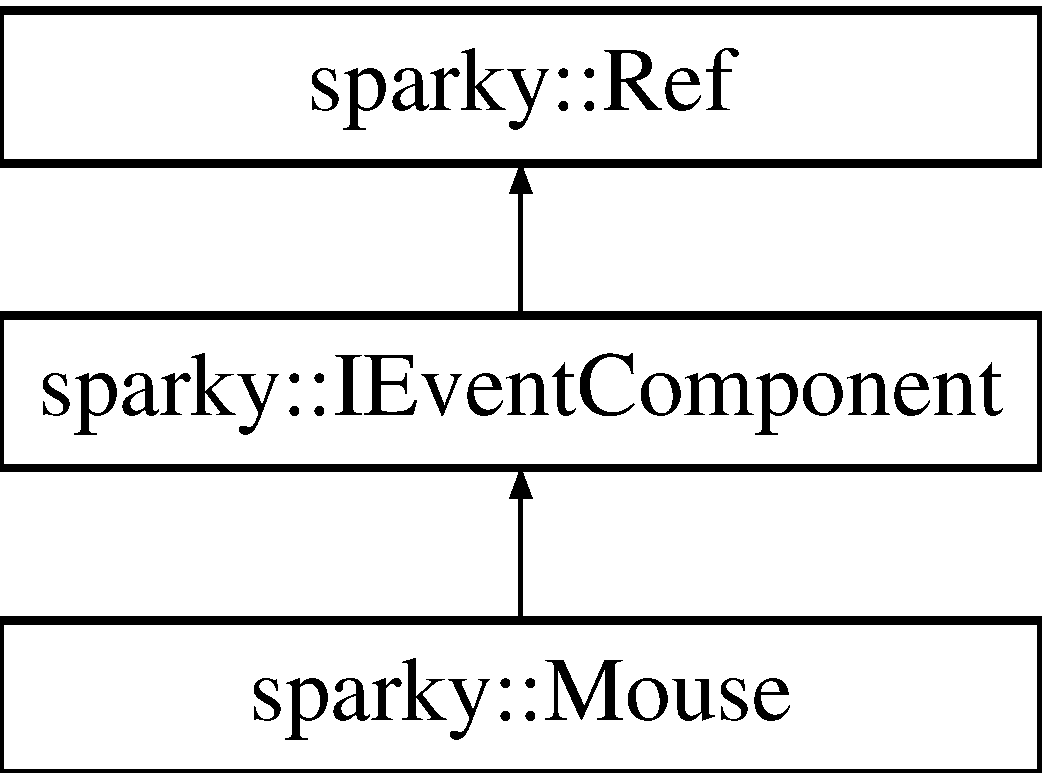
\includegraphics[height=3.000000cm]{classsparky_1_1_mouse}
\end{center}
\end{figure}
\subsection*{Public Member Functions}
\begin{DoxyCompactItemize}
\item 
\hyperlink{classsparky_1_1_mouse_ae4d9c6a668bff6078e538ba79ebd2a56}{Mouse} (void)
\begin{DoxyCompactList}\small\item\em Default constructor of the \hyperlink{classsparky_1_1_mouse}{Mouse} object. \end{DoxyCompactList}\item 
\hyperlink{classsparky_1_1_mouse_a586c420b857867aca1c3d7f4cfee7b9f}{$\sim$\+Mouse} (void)=default\hypertarget{classsparky_1_1_mouse_a586c420b857867aca1c3d7f4cfee7b9f}{}\label{classsparky_1_1_mouse_a586c420b857867aca1c3d7f4cfee7b9f}

\begin{DoxyCompactList}\small\item\em Default destructor of the \hyperlink{classsparky_1_1_mouse}{Mouse} object. \end{DoxyCompactList}\item 
const \hyperlink{classsparky_1_1_vector2}{Vector2i} \& \hyperlink{classsparky_1_1_mouse_aa8da85cc079222bccdd15d74e92b89af}{get\+Position} (void) const 
\begin{DoxyCompactList}\small\item\em Retrieves the current position of the \hyperlink{classsparky_1_1_mouse}{Mouse} object. \end{DoxyCompactList}\item 
const \hyperlink{classsparky_1_1_vector2}{Vector2i} \& \hyperlink{classsparky_1_1_mouse_ad488d7a41b63737baf4e4e7a398d2db2}{get\+Delta} (void) const 
\begin{DoxyCompactList}\small\item\em Retrieves the delta movement of the \hyperlink{classsparky_1_1_mouse}{Mouse} object. \end{DoxyCompactList}\item 
bool \hyperlink{classsparky_1_1_mouse_ac4ed3ae2df7d0a0d01f3fae6a0f0325f}{get\+Button} (const e\+Mouse\+Button button)
\begin{DoxyCompactList}\small\item\em Retrieves the state of the \hyperlink{classsparky_1_1_mouse}{Mouse} button. \end{DoxyCompactList}\item 
bool \hyperlink{classsparky_1_1_mouse_acb7c74fe43bfb85d9b8f94c25024cdc0}{get\+Button\+Down} (const e\+Mouse\+Button button)
\begin{DoxyCompactList}\small\item\em Retrieves the state of the \hyperlink{classsparky_1_1_mouse}{Mouse} button. \end{DoxyCompactList}\item 
bool \hyperlink{classsparky_1_1_mouse_a52f0c26e5f444050400fc1c44aac00e4}{get\+Button\+Up} (const e\+Mouse\+Button button)
\begin{DoxyCompactList}\small\item\em Retrieves the state of the \hyperlink{classsparky_1_1_mouse}{Mouse} button. \end{DoxyCompactList}\item 
void \hyperlink{classsparky_1_1_mouse_a92e5375b15d10af6ea4d3f29f9b373bd}{update} (const S\+D\+L\+\_\+\+Event \&e) override
\begin{DoxyCompactList}\small\item\em Updates the events of the \hyperlink{classsparky_1_1_mouse}{Mouse} object. \end{DoxyCompactList}\end{DoxyCompactItemize}
\subsection*{Additional Inherited Members}


\subsection{Detailed Description}
\hyperlink{classsparky_1_1_mouse}{sparky\+::\+Mouse} is an event component class that is responsible for reading \hyperlink{classsparky_1_1_mouse}{Mouse} buttons and \hyperlink{classsparky_1_1_mouse}{Mouse} states from the \hyperlink{classsparky_1_1_mouse}{Mouse}. \hyperlink{classsparky_1_1_mouse}{sparky\+::\+Mouse} has different methods for different interactions with the \hyperlink{classsparky_1_1_mouse}{Mouse}, such as checking when a button has first been pressed, held down, or released.

As \hyperlink{classsparky_1_1_mouse}{sparky\+::\+Mouse} is an event component the events of \hyperlink{classsparky_1_1_mouse}{sparky\+::\+Mouse} are polled in the event manager singleton, therefore the user does need to worry about polling the system themselves. Below is a code example.

Usage example\+: 
\begin{DoxyCode}
\textcolor{comment}{// Create a Mouse object.}
\hyperlink{classsparky_1_1_mouse}{sparky::Mouse}* pMouse = \textcolor{keyword}{new} \hyperlink{classsparky_1_1_mouse}{sparky::Mouse}();

\textcolor{comment}{// if the left Mouse button has been released, print a message.}
\textcolor{keywordflow}{if} (pMouse->\hyperlink{classsparky_1_1_mouse_a52f0c26e5f444050400fc1c44aac00e4}{getButtonUp}(eMouseButton::LEFT))
\{
    std::cout << \textcolor{stringliteral}{"Left button released!"} << std::endl;
\}
\end{DoxyCode}
 

\subsection{Constructor \& Destructor Documentation}
\index{sparky\+::\+Mouse@{sparky\+::\+Mouse}!Mouse@{Mouse}}
\index{Mouse@{Mouse}!sparky\+::\+Mouse@{sparky\+::\+Mouse}}
\subsubsection[{\texorpdfstring{Mouse(void)}{Mouse(void)}}]{\setlength{\rightskip}{0pt plus 5cm}sparky\+::\+Mouse\+::\+Mouse (
\begin{DoxyParamCaption}
\item[{void}]{}
\end{DoxyParamCaption}
)}\hypertarget{classsparky_1_1_mouse_ae4d9c6a668bff6078e538ba79ebd2a56}{}\label{classsparky_1_1_mouse_ae4d9c6a668bff6078e538ba79ebd2a56}


Default constructor of the \hyperlink{classsparky_1_1_mouse}{Mouse} object. 

All of the member variables are set to false to default values. 

\subsection{Member Function Documentation}
\index{sparky\+::\+Mouse@{sparky\+::\+Mouse}!get\+Button@{get\+Button}}
\index{get\+Button@{get\+Button}!sparky\+::\+Mouse@{sparky\+::\+Mouse}}
\subsubsection[{\texorpdfstring{get\+Button(const e\+Mouse\+Button button)}{getButton(const eMouseButton button)}}]{\setlength{\rightskip}{0pt plus 5cm}bool sparky\+::\+Mouse\+::get\+Button (
\begin{DoxyParamCaption}
\item[{const e\+Mouse\+Button}]{button}
\end{DoxyParamCaption}
)}\hypertarget{classsparky_1_1_mouse_ac4ed3ae2df7d0a0d01f3fae6a0f0325f}{}\label{classsparky_1_1_mouse_ac4ed3ae2df7d0a0d01f3fae6a0f0325f}


Retrieves the state of the \hyperlink{classsparky_1_1_mouse}{Mouse} button. 

Get button will return true continuously whilst the button is held down.


\begin{DoxyRetVals}{Return values}
{\em bool} & The state of the specified button. \\
\hline
\end{DoxyRetVals}
\index{sparky\+::\+Mouse@{sparky\+::\+Mouse}!get\+Button\+Down@{get\+Button\+Down}}
\index{get\+Button\+Down@{get\+Button\+Down}!sparky\+::\+Mouse@{sparky\+::\+Mouse}}
\subsubsection[{\texorpdfstring{get\+Button\+Down(const e\+Mouse\+Button button)}{getButtonDown(const eMouseButton button)}}]{\setlength{\rightskip}{0pt plus 5cm}bool sparky\+::\+Mouse\+::get\+Button\+Down (
\begin{DoxyParamCaption}
\item[{const e\+Mouse\+Button}]{button}
\end{DoxyParamCaption}
)}\hypertarget{classsparky_1_1_mouse_acb7c74fe43bfb85d9b8f94c25024cdc0}{}\label{classsparky_1_1_mouse_acb7c74fe43bfb85d9b8f94c25024cdc0}


Retrieves the state of the \hyperlink{classsparky_1_1_mouse}{Mouse} button. 

Get button down will return true once at the beginning pf the frame when the button is pressed.


\begin{DoxyRetVals}{Return values}
{\em bool} & The state of the specified button. \\
\hline
\end{DoxyRetVals}
\index{sparky\+::\+Mouse@{sparky\+::\+Mouse}!get\+Button\+Up@{get\+Button\+Up}}
\index{get\+Button\+Up@{get\+Button\+Up}!sparky\+::\+Mouse@{sparky\+::\+Mouse}}
\subsubsection[{\texorpdfstring{get\+Button\+Up(const e\+Mouse\+Button button)}{getButtonUp(const eMouseButton button)}}]{\setlength{\rightskip}{0pt plus 5cm}bool sparky\+::\+Mouse\+::get\+Button\+Up (
\begin{DoxyParamCaption}
\item[{const e\+Mouse\+Button}]{button}
\end{DoxyParamCaption}
)}\hypertarget{classsparky_1_1_mouse_a52f0c26e5f444050400fc1c44aac00e4}{}\label{classsparky_1_1_mouse_a52f0c26e5f444050400fc1c44aac00e4}


Retrieves the state of the \hyperlink{classsparky_1_1_mouse}{Mouse} button. 

Get button will return true only when the specified button has been released.


\begin{DoxyRetVals}{Return values}
{\em bool} & The state of the specified button. \\
\hline
\end{DoxyRetVals}
\index{sparky\+::\+Mouse@{sparky\+::\+Mouse}!get\+Delta@{get\+Delta}}
\index{get\+Delta@{get\+Delta}!sparky\+::\+Mouse@{sparky\+::\+Mouse}}
\subsubsection[{\texorpdfstring{get\+Delta(void) const }{getDelta(void) const }}]{\setlength{\rightskip}{0pt plus 5cm}const {\bf Vector2i}\& sparky\+::\+Mouse\+::get\+Delta (
\begin{DoxyParamCaption}
\item[{void}]{}
\end{DoxyParamCaption}
) const}\hypertarget{classsparky_1_1_mouse_ad488d7a41b63737baf4e4e7a398d2db2}{}\label{classsparky_1_1_mouse_ad488d7a41b63737baf4e4e7a398d2db2}


Retrieves the delta movement of the \hyperlink{classsparky_1_1_mouse}{Mouse} object. 

The delta is the amount the \hyperlink{classsparky_1_1_mouse}{Mouse} has moved between the current frame. and previous frame.


\begin{DoxyRetVals}{Return values}
{\em Vector2i\&} & The delta of the \hyperlink{classsparky_1_1_mouse}{Mouse} object. \\
\hline
\end{DoxyRetVals}
\index{sparky\+::\+Mouse@{sparky\+::\+Mouse}!get\+Position@{get\+Position}}
\index{get\+Position@{get\+Position}!sparky\+::\+Mouse@{sparky\+::\+Mouse}}
\subsubsection[{\texorpdfstring{get\+Position(void) const }{getPosition(void) const }}]{\setlength{\rightskip}{0pt plus 5cm}const {\bf Vector2i}\& sparky\+::\+Mouse\+::get\+Position (
\begin{DoxyParamCaption}
\item[{void}]{}
\end{DoxyParamCaption}
) const}\hypertarget{classsparky_1_1_mouse_aa8da85cc079222bccdd15d74e92b89af}{}\label{classsparky_1_1_mouse_aa8da85cc079222bccdd15d74e92b89af}


Retrieves the current position of the \hyperlink{classsparky_1_1_mouse}{Mouse} object. 


\begin{DoxyRetVals}{Return values}
{\em Vector2i\&} & The position of the \hyperlink{classsparky_1_1_mouse}{Mouse}. \\
\hline
\end{DoxyRetVals}
\index{sparky\+::\+Mouse@{sparky\+::\+Mouse}!update@{update}}
\index{update@{update}!sparky\+::\+Mouse@{sparky\+::\+Mouse}}
\subsubsection[{\texorpdfstring{update(const S\+D\+L\+\_\+\+Event \&e) override}{update(const SDL_Event &e) override}}]{\setlength{\rightskip}{0pt plus 5cm}void sparky\+::\+Mouse\+::update (
\begin{DoxyParamCaption}
\item[{const S\+D\+L\+\_\+\+Event \&}]{e}
\end{DoxyParamCaption}
)\hspace{0.3cm}{\ttfamily [override]}, {\ttfamily [virtual]}}\hypertarget{classsparky_1_1_mouse_a92e5375b15d10af6ea4d3f29f9b373bd}{}\label{classsparky_1_1_mouse_a92e5375b15d10af6ea4d3f29f9b373bd}


Updates the events of the \hyperlink{classsparky_1_1_mouse}{Mouse} object. 


\begin{DoxyParams}{Parameters}
{\em e} & The S\+D\+L\+\_\+\+Event being passed in from the Event Manager. \\
\hline
\end{DoxyParams}


Implements \hyperlink{classsparky_1_1_i_event_component_a061c2e74b185caa2b02bc514c5a1544f}{sparky\+::\+I\+Event\+Component}.



The documentation for this class was generated from the following file\+:\begin{DoxyCompactItemize}
\item 
C\+:/\+Users/\+Ben/\+Documents/repos/sparky/include/sparky/input/mouse.\+hpp\end{DoxyCompactItemize}

\hypertarget{classsparky_1_1_point_light}{}\section{sparky\+:\+:Point\+Light Class Reference}
\label{classsparky_1_1_point_light}\index{sparky\+::\+Point\+Light@{sparky\+::\+Point\+Light}}


{\ttfamily \#include $<$pointlight.\+hpp$>$}

Inheritance diagram for sparky\+:\+:Point\+Light\+:\begin{figure}[H]
\begin{center}
\leavevmode
\includegraphics[height=3.000000cm]{classsparky_1_1_point_light}
\end{center}
\end{figure}
\subsection*{Public Member Functions}
\begin{DoxyCompactItemize}
\item 
\hyperlink{classsparky_1_1_point_light_ad0fb91a5dfee3959efefc703f364cb4c}{Point\+Light} (const \hyperlink{structsparky_1_1_s_p_a_r_k_y___p_o_i_n_t___l_i_g_h_t___d_e_s_c}{S\+P\+A\+R\+K\+Y\+\_\+\+P\+O\+I\+N\+T\+\_\+\+L\+I\+G\+H\+T\+\_\+\+D\+E\+SC} \&desc)
\begin{DoxyCompactList}\small\item\em Constructs a \hyperlink{classsparky_1_1_point_light}{Point\+Light} object from a description. \end{DoxyCompactList}\item 
\hyperlink{classsparky_1_1_point_light_a048dc877951ef45dd84e725d956e844a}{$\sim$\+Point\+Light} (void)=default\hypertarget{classsparky_1_1_point_light_a048dc877951ef45dd84e725d956e844a}{}\label{classsparky_1_1_point_light_a048dc877951ef45dd84e725d956e844a}

\begin{DoxyCompactList}\small\item\em Default destructor of the \hyperlink{classsparky_1_1_point_light}{Point\+Light} object. \end{DoxyCompactList}\item 
const \hyperlink{structsparky_1_1_attenuation}{Attenuation} \& \hyperlink{classsparky_1_1_point_light_ad7c189e15b39edc5ebb4de54a156e435}{get\+Attenuation} (void) const 
\begin{DoxyCompactList}\small\item\em Retrieves the attenuation of this \hyperlink{classsparky_1_1_point_light}{Point\+Light}. \end{DoxyCompactList}\item 
void \hyperlink{classsparky_1_1_point_light_aa03adb581601b178ff0058ad18af1ec9}{set\+Attenuation} (const \hyperlink{structsparky_1_1_attenuation}{Attenuation} \&attenuation)
\begin{DoxyCompactList}\small\item\em Sets the attenuation of the \hyperlink{classsparky_1_1_point_light}{Point\+Light}. \end{DoxyCompactList}\item 
float \hyperlink{classsparky_1_1_point_light_aaf453df6857c6dfc6e50c08adaf40184}{get\+Range} (void) const 
\begin{DoxyCompactList}\small\item\em Retrieves the range of the \hyperlink{classsparky_1_1_point_light}{Point\+Light}. \end{DoxyCompactList}\item 
void \hyperlink{classsparky_1_1_point_light_ab82fe8464f26b87ab595a2a9bfc14281}{set\+Range} (const float range)
\begin{DoxyCompactList}\small\item\em Sets the maximum radius of the \hyperlink{classsparky_1_1_point_light}{Point\+Light}. \end{DoxyCompactList}\item 
void \hyperlink{classsparky_1_1_point_light_a09d074c94750d1bf892eaf2e757d1aec}{set\+Uniforms} (\hyperlink{classsparky_1_1_uniform}{Uniform} \&uniform)
\begin{DoxyCompactList}\small\item\em Sets the uniform variables of a \hyperlink{classsparky_1_1_point_light}{Point\+Light} within a shader. \end{DoxyCompactList}\item 
void \hyperlink{classsparky_1_1_point_light_a12ff1a240f2ad0e91a12e57e1c6ed7e7}{add\+Light} (void) override
\begin{DoxyCompactList}\small\item\em Adds the light to the current pipeline if the conditions are correct. \end{DoxyCompactList}\end{DoxyCompactItemize}
\subsection*{Additional Inherited Members}


\subsection{Detailed Description}
\hyperlink{classsparky_1_1_point_light}{sparky\+::\+Point\+Light} is a light based component of the Sparky Engine. A \hyperlink{classsparky_1_1_point_light}{Point\+Light} can be used to represent a \hyperlink{classsparky_1_1_light}{Light} source with a specific radius of effect, such as a lantern or torch on a wall.

Similar to other lights within the application, it uses descriptions to define it\textquotesingle{}s behaviour. Below is a code example.

Usage example\+: 
\begin{DoxyCode}
\textcolor{comment}{// Create a description and "zero" it out.}
\hyperlink{structsparky_1_1_s_p_a_r_k_y___p_o_i_n_t___l_i_g_h_t___d_e_s_c}{sparky::SPARKY\_POINT\_LIGHT\_DESC} desc;
memset(&desc, 0, \textcolor{keyword}{sizeof}(\hyperlink{structsparky_1_1_s_p_a_r_k_y___p_o_i_n_t___l_i_g_h_t___d_e_s_c}{sparky::SPARKY\_POINT\_LIGHT\_DESC}));

\textcolor{comment}{// Set the information of the description.}
desc.\hyperlink{structsparky_1_1_s_p_a_r_k_y___p_o_i_n_t___l_i_g_h_t___d_e_s_c_ab07cf32717f09f5a977e5f760961fb4a}{base}.\hyperlink{structsparky_1_1_s_p_a_r_k_y___b_a_s_e___l_i_g_h_t___d_e_s_c_a0b3e29108f714a6004fca8e4a1d6cf67}{name} = \textcolor{stringliteral}{"u\_light"};
desc.\hyperlink{structsparky_1_1_s_p_a_r_k_y___p_o_i_n_t___l_i_g_h_t___d_e_s_c_ab07cf32717f09f5a977e5f760961fb4a}{base}.\hyperlink{structsparky_1_1_s_p_a_r_k_y___b_a_s_e___l_i_g_h_t___d_e_s_c_aed72b3ed8f00100cee86d32063909a48}{position} = \hyperlink{classsparky_1_1_vector3_accf83dce35ce0cd7aeeb865fe3e9e7a9}{sparky::Vector3f::zero}();
desc.\hyperlink{structsparky_1_1_s_p_a_r_k_y___p_o_i_n_t___l_i_g_h_t___d_e_s_c_ab07cf32717f09f5a977e5f760961fb4a}{base}.\hyperlink{structsparky_1_1_s_p_a_r_k_y___b_a_s_e___l_i_g_h_t___d_e_s_c_a87e733aa6c7f8cecf430e5d09f424035}{colour} = \hyperlink{classsparky_1_1_vector3}{sparky::Vector3f}(0.5f, 0.0f, 0.0f);
desc.\hyperlink{structsparky_1_1_s_p_a_r_k_y___p_o_i_n_t___l_i_g_h_t___d_e_s_c_ab07cf32717f09f5a977e5f760961fb4a}{base}.\hyperlink{structsparky_1_1_s_p_a_r_k_y___b_a_s_e___l_i_g_h_t___d_e_s_c_a3e2f83fe7f13727f235e957debb54634}{intensity} = 0.8f;

desc.\hyperlink{structsparky_1_1_s_p_a_r_k_y___p_o_i_n_t___l_i_g_h_t___d_e_s_c_a61495a6dedb077e939aea5be9cd72619}{attenuation}.\hyperlink{structsparky_1_1_attenuation_a0bbefcc87e251c6bdbd34f889e2906ce}{constant} = 1.0f;
desc.\hyperlink{structsparky_1_1_s_p_a_r_k_y___p_o_i_n_t___l_i_g_h_t___d_e_s_c_a61495a6dedb077e939aea5be9cd72619}{attenuation}.\hyperlink{structsparky_1_1_attenuation_a2cd5cc43f8b4495b399037a94c30ffea}{linear} = 0.7f;
desc.\hyperlink{structsparky_1_1_s_p_a_r_k_y___p_o_i_n_t___l_i_g_h_t___d_e_s_c_a61495a6dedb077e939aea5be9cd72619}{attenuation}.\hyperlink{structsparky_1_1_attenuation_ad2b6be370c7b71c9755903db2506a49f}{exponent} = 1.8f;

desc.\hyperlink{structsparky_1_1_s_p_a_r_k_y___p_o_i_n_t___l_i_g_h_t___d_e_s_c_a1aa05df10bea864c48c19df36c877281}{range} = 15.0f;

\textcolor{comment}{// Create a light with the description and retain.}
\hyperlink{classsparky_1_1_point_light}{sparky::PointLight}* pLight = \textcolor{keyword}{new} \hyperlink{classsparky_1_1_point_light}{sparky::PointLight}(desc);
pLight->\hyperlink{classsparky_1_1_ref_aeeb606836c315aa3b8a2254e23eb0899}{addRef}();

\textcolor{comment}{// Update the uniforms within a shader object.}
pLight->\hyperlink{classsparky_1_1_point_light_a09d074c94750d1bf892eaf2e757d1aec}{setUniforms}(m\_uniform);
\end{DoxyCode}
 

\subsection{Constructor \& Destructor Documentation}
\index{sparky\+::\+Point\+Light@{sparky\+::\+Point\+Light}!Point\+Light@{Point\+Light}}
\index{Point\+Light@{Point\+Light}!sparky\+::\+Point\+Light@{sparky\+::\+Point\+Light}}
\subsubsection[{\texorpdfstring{Point\+Light(const S\+P\+A\+R\+K\+Y\+\_\+\+P\+O\+I\+N\+T\+\_\+\+L\+I\+G\+H\+T\+\_\+\+D\+E\+S\+C \&desc)}{PointLight(const SPARKY_POINT_LIGHT_DESC &desc)}}]{\setlength{\rightskip}{0pt plus 5cm}sparky\+::\+Point\+Light\+::\+Point\+Light (
\begin{DoxyParamCaption}
\item[{const {\bf S\+P\+A\+R\+K\+Y\+\_\+\+P\+O\+I\+N\+T\+\_\+\+L\+I\+G\+H\+T\+\_\+\+D\+E\+SC} \&}]{desc}
\end{DoxyParamCaption}
)\hspace{0.3cm}{\ttfamily [explicit]}}\hypertarget{classsparky_1_1_point_light_ad0fb91a5dfee3959efefc703f364cb4c}{}\label{classsparky_1_1_point_light_ad0fb91a5dfee3959efefc703f364cb4c}


Constructs a \hyperlink{classsparky_1_1_point_light}{Point\+Light} object from a description. 

The description will define the behaviour of this \hyperlink{classsparky_1_1_point_light}{Point\+Light}. The members of the class will be set to those within the description and applied within the shader.


\begin{DoxyParams}{Parameters}
{\em desc} & The description of the \hyperlink{classsparky_1_1_point_light}{Point\+Light} object. \\
\hline
\end{DoxyParams}


\subsection{Member Function Documentation}
\index{sparky\+::\+Point\+Light@{sparky\+::\+Point\+Light}!add\+Light@{add\+Light}}
\index{add\+Light@{add\+Light}!sparky\+::\+Point\+Light@{sparky\+::\+Point\+Light}}
\subsubsection[{\texorpdfstring{add\+Light(void) override}{addLight(void) override}}]{\setlength{\rightskip}{0pt plus 5cm}void sparky\+::\+Point\+Light\+::add\+Light (
\begin{DoxyParamCaption}
\item[{void}]{}
\end{DoxyParamCaption}
)\hspace{0.3cm}{\ttfamily [override]}, {\ttfamily [virtual]}}\hypertarget{classsparky_1_1_point_light_a12ff1a240f2ad0e91a12e57e1c6ed7e7}{}\label{classsparky_1_1_point_light_a12ff1a240f2ad0e91a12e57e1c6ed7e7}


Adds the light to the current pipeline if the conditions are correct. 

For Point Lights their position and radius is checked using the sphere check in the \hyperlink{classsparky_1_1_frustum}{Frustum} class. If they are currently within view, they are added to the \hyperlink{classsparky_1_1_game_manager}{Game\+Manager} for rendering this frame. 

Implements \hyperlink{classsparky_1_1_light_a23e37022528ba94549b89b99d2848eb2}{sparky\+::\+Light}.

\index{sparky\+::\+Point\+Light@{sparky\+::\+Point\+Light}!get\+Attenuation@{get\+Attenuation}}
\index{get\+Attenuation@{get\+Attenuation}!sparky\+::\+Point\+Light@{sparky\+::\+Point\+Light}}
\subsubsection[{\texorpdfstring{get\+Attenuation(void) const }{getAttenuation(void) const }}]{\setlength{\rightskip}{0pt plus 5cm}const {\bf Attenuation}\& sparky\+::\+Point\+Light\+::get\+Attenuation (
\begin{DoxyParamCaption}
\item[{void}]{}
\end{DoxyParamCaption}
) const}\hypertarget{classsparky_1_1_point_light_ad7c189e15b39edc5ebb4de54a156e435}{}\label{classsparky_1_1_point_light_ad7c189e15b39edc5ebb4de54a156e435}


Retrieves the attenuation of this \hyperlink{classsparky_1_1_point_light}{Point\+Light}. 

The attenuation refers to the reduction or \char`\"{}fall-\/off\char`\"{} of the light over a distance.


\begin{DoxyRetVals}{Return values}
{\em \hyperlink{structsparky_1_1_attenuation}{Attenuation}} & The \hyperlink{structsparky_1_1_attenuation}{Attenuation} of the \hyperlink{classsparky_1_1_point_light}{Point\+Light}. \\
\hline
\end{DoxyRetVals}
\index{sparky\+::\+Point\+Light@{sparky\+::\+Point\+Light}!get\+Range@{get\+Range}}
\index{get\+Range@{get\+Range}!sparky\+::\+Point\+Light@{sparky\+::\+Point\+Light}}
\subsubsection[{\texorpdfstring{get\+Range(void) const }{getRange(void) const }}]{\setlength{\rightskip}{0pt plus 5cm}float sparky\+::\+Point\+Light\+::get\+Range (
\begin{DoxyParamCaption}
\item[{void}]{}
\end{DoxyParamCaption}
) const}\hypertarget{classsparky_1_1_point_light_aaf453df6857c6dfc6e50c08adaf40184}{}\label{classsparky_1_1_point_light_aaf453df6857c6dfc6e50c08adaf40184}


Retrieves the range of the \hyperlink{classsparky_1_1_point_light}{Point\+Light}. 

The range refers to the maximum radius of effect that this \hyperlink{classsparky_1_1_point_light}{Point\+Light} will have on any geometry within the scene.


\begin{DoxyRetVals}{Return values}
{\em float} & The range of the \hyperlink{classsparky_1_1_point_light}{Point\+Light}. \\
\hline
\end{DoxyRetVals}
\index{sparky\+::\+Point\+Light@{sparky\+::\+Point\+Light}!set\+Attenuation@{set\+Attenuation}}
\index{set\+Attenuation@{set\+Attenuation}!sparky\+::\+Point\+Light@{sparky\+::\+Point\+Light}}
\subsubsection[{\texorpdfstring{set\+Attenuation(const Attenuation \&attenuation)}{setAttenuation(const Attenuation &attenuation)}}]{\setlength{\rightskip}{0pt plus 5cm}void sparky\+::\+Point\+Light\+::set\+Attenuation (
\begin{DoxyParamCaption}
\item[{const {\bf Attenuation} \&}]{attenuation}
\end{DoxyParamCaption}
)}\hypertarget{classsparky_1_1_point_light_aa03adb581601b178ff0058ad18af1ec9}{}\label{classsparky_1_1_point_light_aa03adb581601b178ff0058ad18af1ec9}


Sets the attenuation of the \hyperlink{classsparky_1_1_point_light}{Point\+Light}. 

The attenuation refers to the reduction or \char`\"{}fall-\/off\char`\"{} of the light over a distance.


\begin{DoxyParams}{Parameters}
{\em attenuation} & The new attenuation of the \hyperlink{classsparky_1_1_point_light}{Point\+Light}. \\
\hline
\end{DoxyParams}
\index{sparky\+::\+Point\+Light@{sparky\+::\+Point\+Light}!set\+Range@{set\+Range}}
\index{set\+Range@{set\+Range}!sparky\+::\+Point\+Light@{sparky\+::\+Point\+Light}}
\subsubsection[{\texorpdfstring{set\+Range(const float range)}{setRange(const float range)}}]{\setlength{\rightskip}{0pt plus 5cm}void sparky\+::\+Point\+Light\+::set\+Range (
\begin{DoxyParamCaption}
\item[{const float}]{range}
\end{DoxyParamCaption}
)}\hypertarget{classsparky_1_1_point_light_ab82fe8464f26b87ab595a2a9bfc14281}{}\label{classsparky_1_1_point_light_ab82fe8464f26b87ab595a2a9bfc14281}


Sets the maximum radius of the \hyperlink{classsparky_1_1_point_light}{Point\+Light}. 

The range refers to the maximum radius of effect that this \hyperlink{classsparky_1_1_point_light}{Point\+Light} will have on any geometry within the scene.


\begin{DoxyParams}{Parameters}
{\em range} & The new maximum range of the \hyperlink{classsparky_1_1_point_light}{Point\+Light}. \\
\hline
\end{DoxyParams}
\index{sparky\+::\+Point\+Light@{sparky\+::\+Point\+Light}!set\+Uniforms@{set\+Uniforms}}
\index{set\+Uniforms@{set\+Uniforms}!sparky\+::\+Point\+Light@{sparky\+::\+Point\+Light}}
\subsubsection[{\texorpdfstring{set\+Uniforms(\+Uniform \&uniform)}{setUniforms(Uniform &uniform)}}]{\setlength{\rightskip}{0pt plus 5cm}void sparky\+::\+Point\+Light\+::set\+Uniforms (
\begin{DoxyParamCaption}
\item[{{\bf Uniform} \&}]{uniform}
\end{DoxyParamCaption}
)}\hypertarget{classsparky_1_1_point_light_a09d074c94750d1bf892eaf2e757d1aec}{}\label{classsparky_1_1_point_light_a09d074c94750d1bf892eaf2e757d1aec}


Sets the uniform variables of a \hyperlink{classsparky_1_1_point_light}{Point\+Light} within a shader. 

Whenever a \hyperlink{classsparky_1_1_point_light}{Point\+Light} is used within a shader, the variables of the \hyperlink{classsparky_1_1_point_light}{Point\+Light} must be updated for correct shading behaviour.


\begin{DoxyParams}{Parameters}
{\em uniform} & The Uniforms of the currently bound shader. \\
\hline
\end{DoxyParams}


The documentation for this class was generated from the following file\+:\begin{DoxyCompactItemize}
\item 
C\+:/\+Users/\+Ben/\+Documents/repos/sparky/include/sparky/lighting/pointlight.\+hpp\end{DoxyCompactItemize}

\hypertarget{classsparky_1_1_point_shader}{}\section{sparky\+:\+:Point\+Shader Class Reference}
\label{classsparky_1_1_point_shader}\index{sparky\+::\+Point\+Shader@{sparky\+::\+Point\+Shader}}


{\ttfamily \#include $<$pointshader.\+hpp$>$}

Inheritance diagram for sparky\+:\+:Point\+Shader\+:\begin{figure}[H]
\begin{center}
\leavevmode
\includegraphics[height=3.000000cm]{classsparky_1_1_point_shader}
\end{center}
\end{figure}
\subsection*{Public Member Functions}
\begin{DoxyCompactItemize}
\item 
\hyperlink{classsparky_1_1_point_shader_a76657c1a0653f9521bf25fcece5c004f}{Point\+Shader} (void)
\begin{DoxyCompactList}\small\item\em Default constructor of the \hyperlink{classsparky_1_1_point_shader}{Point\+Shader} object. \end{DoxyCompactList}\item 
\hyperlink{classsparky_1_1_point_shader_affc386eeb79d33dceb4beee4a25c0004}{$\sim$\+Point\+Shader} (void)=default\hypertarget{classsparky_1_1_point_shader_affc386eeb79d33dceb4beee4a25c0004}{}\label{classsparky_1_1_point_shader_affc386eeb79d33dceb4beee4a25c0004}

\begin{DoxyCompactList}\small\item\em Default destructor of the Point Shader object. \end{DoxyCompactList}\item 
void \hyperlink{classsparky_1_1_point_shader_a2060a2423cf2aed74c6944d777557ba9}{set\+Active\+Light} (\hyperlink{classsparky_1_1_point_light}{Point\+Light} $\ast$p\+Light)
\begin{DoxyCompactList}\small\item\em Sets the currently active point light of the multi-\/pass rendering pipeline. \end{DoxyCompactList}\item 
void \hyperlink{classsparky_1_1_point_shader_a96b31364d736885500c7af9615ed11bd}{update} (const \hyperlink{classsparky_1_1_transform}{Transform} \&transform) override
\begin{DoxyCompactList}\small\item\em Updates the uniforms of the point light shader. \end{DoxyCompactList}\end{DoxyCompactItemize}
\subsection*{Additional Inherited Members}


\subsection{Detailed Description}
\hyperlink{classsparky_1_1_point_shader}{sparky\+::\+Point\+Shader} is one of the shaders used within the applications multi-\/pass rendering pipeline. It is responsible for rendering the effects of point lights onto geometry.

\hyperlink{classsparky_1_1_point_shader}{sparky\+::\+Point\+Shader} never has to be used implicitly by the user, instead it is utilised to render the lights of the scene within the \hyperlink{classsparky_1_1_game_manager}{Game\+Manager} singleton class. Below is a code example.

Usage example\+: 
\begin{DoxyCode}
\textcolor{comment}{// Get a shader from the resource manager.}
\hyperlink{classsparky_1_1_point_shader}{sparky::PointShader} pShader = 
      \hyperlink{classsparky_1_1_singleton_a8e56848cf24e5f4cdcd493c64d576f10}{sparky::ResourceManager::getInstance}().
      \hyperlink{classsparky_1_1_resource_manager_a8d48e497254410edf301df3d08248520}{getShader}<\hyperlink{classsparky_1_1_point_shader}{sparky::PointShader}>(\textcolor{stringliteral}{"point"});

\textcolor{comment}{// Create a transform.}
\hyperlink{classsparky_1_1_transform}{sparky::Transform} t;
t.\hyperlink{classsparky_1_1_transform_aff16fd5ad2157d604364a59835865d5c}{setPosition}(0.0f, 0.0f, 5.0f);

\textcolor{comment}{// Pass the transform to the shader.}
pShader->\hyperlink{classsparky_1_1_point_shader_a96b31364d736885500c7af9615ed11bd}{update}(t);
\end{DoxyCode}
 

\subsection{Constructor \& Destructor Documentation}
\index{sparky\+::\+Point\+Shader@{sparky\+::\+Point\+Shader}!Point\+Shader@{Point\+Shader}}
\index{Point\+Shader@{Point\+Shader}!sparky\+::\+Point\+Shader@{sparky\+::\+Point\+Shader}}
\subsubsection[{\texorpdfstring{Point\+Shader(void)}{PointShader(void)}}]{\setlength{\rightskip}{0pt plus 5cm}sparky\+::\+Point\+Shader\+::\+Point\+Shader (
\begin{DoxyParamCaption}
\item[{void}]{}
\end{DoxyParamCaption}
)\hspace{0.3cm}{\ttfamily [explicit]}}\hypertarget{classsparky_1_1_point_shader_a76657c1a0653f9521bf25fcece5c004f}{}\label{classsparky_1_1_point_shader_a76657c1a0653f9521bf25fcece5c004f}


Default constructor of the \hyperlink{classsparky_1_1_point_shader}{Point\+Shader} object. 

The default constructor will bind and compile the two external shaders for use with Point Lights. This shader is used within the multi-\/pass rendering pipeline to render point lights onto geometry. 

\subsection{Member Function Documentation}
\index{sparky\+::\+Point\+Shader@{sparky\+::\+Point\+Shader}!set\+Active\+Light@{set\+Active\+Light}}
\index{set\+Active\+Light@{set\+Active\+Light}!sparky\+::\+Point\+Shader@{sparky\+::\+Point\+Shader}}
\subsubsection[{\texorpdfstring{set\+Active\+Light(\+Point\+Light $\ast$p\+Light)}{setActiveLight(PointLight *pLight)}}]{\setlength{\rightskip}{0pt plus 5cm}void sparky\+::\+Point\+Shader\+::set\+Active\+Light (
\begin{DoxyParamCaption}
\item[{{\bf Point\+Light} $\ast$}]{p\+Light}
\end{DoxyParamCaption}
)}\hypertarget{classsparky_1_1_point_shader_a2060a2423cf2aed74c6944d777557ba9}{}\label{classsparky_1_1_point_shader_a2060a2423cf2aed74c6944d777557ba9}


Sets the currently active point light of the multi-\/pass rendering pipeline. 


\begin{DoxyParams}{Parameters}
{\em p\+Light} & The currently active point light. \\
\hline
\end{DoxyParams}
\index{sparky\+::\+Point\+Shader@{sparky\+::\+Point\+Shader}!update@{update}}
\index{update@{update}!sparky\+::\+Point\+Shader@{sparky\+::\+Point\+Shader}}
\subsubsection[{\texorpdfstring{update(const Transform \&transform) override}{update(const Transform &transform) override}}]{\setlength{\rightskip}{0pt plus 5cm}void sparky\+::\+Point\+Shader\+::update (
\begin{DoxyParamCaption}
\item[{const {\bf Transform} \&}]{transform}
\end{DoxyParamCaption}
)\hspace{0.3cm}{\ttfamily [override]}, {\ttfamily [virtual]}}\hypertarget{classsparky_1_1_point_shader_a96b31364d736885500c7af9615ed11bd}{}\label{classsparky_1_1_point_shader_a96b31364d736885500c7af9615ed11bd}


Updates the uniforms of the point light shader. 

The uniforms updated within this shader is the currently active point light and the normals generated from the deferred rendering pipeline.


\begin{DoxyParams}{Parameters}
{\em transform} & The transform of the currently rendering object. \\
\hline
\end{DoxyParams}


Implements \hyperlink{classsparky_1_1_i_shader_component_a0bf4ef38fcf1ac17fd1852668baeef88}{sparky\+::\+I\+Shader\+Component}.



The documentation for this class was generated from the following file\+:\begin{DoxyCompactItemize}
\item 
C\+:/\+Users/\+Ben/\+Documents/repos/sparky/include/sparky/rendering/pointshader.\+hpp\end{DoxyCompactItemize}

\hypertarget{classsparky_1_1_pool_manager}{}\section{sparky\+:\+:Pool\+Manager Class Reference}
\label{classsparky_1_1_pool_manager}\index{sparky\+::\+Pool\+Manager@{sparky\+::\+Pool\+Manager}}


{\ttfamily \#include $<$pool.\+hpp$>$}

Inheritance diagram for sparky\+:\+:Pool\+Manager\+:\begin{figure}[H]
\begin{center}
\leavevmode
\includegraphics[height=2.000000cm]{classsparky_1_1_pool_manager}
\end{center}
\end{figure}
\subsection*{Public Member Functions}
\begin{DoxyCompactItemize}
\item 
\hyperlink{classsparky_1_1_pool_manager_a3bd0fc1b6f4fb33613bc987ac61114af}{$\sim$\+Pool\+Manager} (void)
\begin{DoxyCompactList}\small\item\em Destructs the \hyperlink{classsparky_1_1_pool_manager}{Pool\+Manager} object instance. \end{DoxyCompactList}\item 
void \hyperlink{classsparky_1_1_pool_manager_aba8de62aa0f13d14ad68d3d26cb9549a}{add\+Object} (\hyperlink{classsparky_1_1_ref}{Ref} $\ast$p\+Object)
\begin{DoxyCompactList}\small\item\em Adds a dynamic object \hyperlink{classsparky_1_1_ref}{Ref} to the pool. \end{DoxyCompactList}\item 
bool \hyperlink{classsparky_1_1_pool_manager_a1c476a4c9d60514a86cb6c4a6e886217}{contains} (\hyperlink{classsparky_1_1_ref}{Ref} $\ast$p\+Object) const 
\begin{DoxyCompactList}\small\item\em Checks to see if the passed in object is currently within the pool. \end{DoxyCompactList}\item 
void \hyperlink{classsparky_1_1_pool_manager_a32fb836cefbcd22763895259779eea65}{flush} (void)
\begin{DoxyCompactList}\small\item\em Flushes the pool of all currently retained \hyperlink{classsparky_1_1_ref}{Ref}\textquotesingle{}s. \end{DoxyCompactList}\end{DoxyCompactItemize}
\subsection*{Friends}
\begin{DoxyCompactItemize}
\item 
class {\bfseries Singleton$<$ Pool\+Manager $>$}\hypertarget{classsparky_1_1_pool_manager_aaa4fa1401745a95c344d924e2e8cd456}{}\label{classsparky_1_1_pool_manager_aaa4fa1401745a95c344d924e2e8cd456}

\end{DoxyCompactItemize}
\subsection*{Additional Inherited Members}


\subsection{Detailed Description}
\hyperlink{classsparky_1_1_pool_manager}{sparky\+::\+Pool\+Manager} is a singleton class that is responsible for the basic garbage collection of Sparky. Dynamic \hyperlink{classsparky_1_1_ref}{Ref} objects are added to the list. At the end of the current frame, each objects reference count is decremented and if the count is 0, it is deleted. 

\subsection{Constructor \& Destructor Documentation}
\index{sparky\+::\+Pool\+Manager@{sparky\+::\+Pool\+Manager}!````~Pool\+Manager@{$\sim$\+Pool\+Manager}}
\index{````~Pool\+Manager@{$\sim$\+Pool\+Manager}!sparky\+::\+Pool\+Manager@{sparky\+::\+Pool\+Manager}}
\subsubsection[{\texorpdfstring{$\sim$\+Pool\+Manager(void)}{~PoolManager(void)}}]{\setlength{\rightskip}{0pt plus 5cm}sparky\+::\+Pool\+Manager\+::$\sim$\+Pool\+Manager (
\begin{DoxyParamCaption}
\item[{void}]{}
\end{DoxyParamCaption}
)}\hypertarget{classsparky_1_1_pool_manager_a3bd0fc1b6f4fb33613bc987ac61114af}{}\label{classsparky_1_1_pool_manager_a3bd0fc1b6f4fb33613bc987ac61114af}


Destructs the \hyperlink{classsparky_1_1_pool_manager}{Pool\+Manager} object instance. 

The flush method is called once more upon the objects destruction to make sure that it is not retaining any objects, therefore preventing memory leaks. 

\subsection{Member Function Documentation}
\index{sparky\+::\+Pool\+Manager@{sparky\+::\+Pool\+Manager}!add\+Object@{add\+Object}}
\index{add\+Object@{add\+Object}!sparky\+::\+Pool\+Manager@{sparky\+::\+Pool\+Manager}}
\subsubsection[{\texorpdfstring{add\+Object(\+Ref $\ast$p\+Object)}{addObject(Ref *pObject)}}]{\setlength{\rightskip}{0pt plus 5cm}void sparky\+::\+Pool\+Manager\+::add\+Object (
\begin{DoxyParamCaption}
\item[{{\bf Ref} $\ast$}]{p\+Object}
\end{DoxyParamCaption}
)}\hypertarget{classsparky_1_1_pool_manager_aba8de62aa0f13d14ad68d3d26cb9549a}{}\label{classsparky_1_1_pool_manager_aba8de62aa0f13d14ad68d3d26cb9549a}


Adds a dynamic object \hyperlink{classsparky_1_1_ref}{Ref} to the pool. 

The object added is retained within the pool until the end of the current frame, where the objects reference count is decremented and cleared from the pool.


\begin{DoxyParams}{Parameters}
{\em p\+Object} & The \hyperlink{classsparky_1_1_ref}{Ref} to add to the pool. \\
\hline
\end{DoxyParams}
\index{sparky\+::\+Pool\+Manager@{sparky\+::\+Pool\+Manager}!contains@{contains}}
\index{contains@{contains}!sparky\+::\+Pool\+Manager@{sparky\+::\+Pool\+Manager}}
\subsubsection[{\texorpdfstring{contains(\+Ref $\ast$p\+Object) const }{contains(Ref *pObject) const }}]{\setlength{\rightskip}{0pt plus 5cm}bool sparky\+::\+Pool\+Manager\+::contains (
\begin{DoxyParamCaption}
\item[{{\bf Ref} $\ast$}]{p\+Object}
\end{DoxyParamCaption}
) const}\hypertarget{classsparky_1_1_pool_manager_a1c476a4c9d60514a86cb6c4a6e886217}{}\label{classsparky_1_1_pool_manager_a1c476a4c9d60514a86cb6c4a6e886217}


Checks to see if the passed in object is currently within the pool. 

This method will search through all of the objects within the current pool and return true if the object parameter has been found.


\begin{DoxyParams}{Parameters}
{\em p\+Object} & The \hyperlink{classsparky_1_1_ref}{Ref} to search the pool for.\\
\hline
\end{DoxyParams}

\begin{DoxyRetVals}{Return values}
{\em bool} & True if the \hyperlink{classsparky_1_1_ref}{Ref} has been found, false if not. \\
\hline
\end{DoxyRetVals}
\index{sparky\+::\+Pool\+Manager@{sparky\+::\+Pool\+Manager}!flush@{flush}}
\index{flush@{flush}!sparky\+::\+Pool\+Manager@{sparky\+::\+Pool\+Manager}}
\subsubsection[{\texorpdfstring{flush(void)}{flush(void)}}]{\setlength{\rightskip}{0pt plus 5cm}void sparky\+::\+Pool\+Manager\+::flush (
\begin{DoxyParamCaption}
\item[{void}]{}
\end{DoxyParamCaption}
)}\hypertarget{classsparky_1_1_pool_manager_a32fb836cefbcd22763895259779eea65}{}\label{classsparky_1_1_pool_manager_a32fb836cefbcd22763895259779eea65}


Flushes the pool of all currently retained \hyperlink{classsparky_1_1_ref}{Ref}\textquotesingle{}s. 

At the end of each frame, the pool is emptied of all retained \hyperlink{classsparky_1_1_ref}{Ref}\textquotesingle{}s, each \hyperlink{classsparky_1_1_ref}{Ref}\textquotesingle{}s reference counter is decremented before flushing. 

The documentation for this class was generated from the following file\+:\begin{DoxyCompactItemize}
\item 
C\+:/\+Users/\+Ben/\+Documents/repos/sparky/include/sparky/core/pool.\+hpp\end{DoxyCompactItemize}

\hypertarget{classsparky_1_1_program}{}\section{sparky\+:\+:Program Class Reference}
\label{classsparky_1_1_program}\index{sparky\+::\+Program@{sparky\+::\+Program}}


{\ttfamily \#include $<$program.\+hpp$>$}

\subsection*{Public Member Functions}
\begin{DoxyCompactItemize}
\item 
\hyperlink{classsparky_1_1_program_a17217a0c5b6404f974aff8b52d33be3c}{Program} (void)\hypertarget{classsparky_1_1_program_a17217a0c5b6404f974aff8b52d33be3c}{}\label{classsparky_1_1_program_a17217a0c5b6404f974aff8b52d33be3c}

\begin{DoxyCompactList}\small\item\em Default construction of the \hyperlink{classsparky_1_1_program}{Program} object. \end{DoxyCompactList}\item 
\hyperlink{classsparky_1_1_program_ae743c5b397c87b9391f465e827c20ef9}{$\sim$\+Program} (void)
\begin{DoxyCompactList}\small\item\em Destruction of the \hyperlink{classsparky_1_1_program}{Program} object. \end{DoxyCompactList}\item 
G\+Luint \hyperlink{classsparky_1_1_program_a111730e41b76cdbf53b37463dd1d5530}{get\+ID} (void) const 
\begin{DoxyCompactList}\small\item\em Retrieves the ID of the \hyperlink{classsparky_1_1_program}{Program} object. \end{DoxyCompactList}\item 
void \hyperlink{classsparky_1_1_program_ac60e7883dc4076f78c3bcc1d5519f7e7}{attach\+Shader} (\hyperlink{classsparky_1_1_g_l_s_l_object}{G\+L\+S\+L\+Object} $\ast$p\+Object)
\begin{DoxyCompactList}\small\item\em Attach a Shader object to the \hyperlink{classsparky_1_1_program}{Program}. \end{DoxyCompactList}\item 
void \hyperlink{classsparky_1_1_program_a7cbc014919fdcca3889edb283fbd4115}{link} (void)
\begin{DoxyCompactList}\small\item\em Link the \hyperlink{classsparky_1_1_program}{Program} object. \end{DoxyCompactList}\item 
void \hyperlink{classsparky_1_1_program_aa61c56e5215ec1cce8d6f7003d883f78}{bind} (void) const 
\begin{DoxyCompactList}\small\item\em Bind the \hyperlink{classsparky_1_1_program}{Program} ID. \end{DoxyCompactList}\item 
void \hyperlink{classsparky_1_1_program_a7682674da3980b52cd2dc0ea0261b867}{unbind} (void) const 
\begin{DoxyCompactList}\small\item\em Unbind the \hyperlink{classsparky_1_1_program}{Program} ID. \end{DoxyCompactList}\end{DoxyCompactItemize}


\subsection{Detailed Description}
The \hyperlink{classsparky_1_1_program}{Program} class is responsible for the linking and joint compilation of all attached shaders. The \hyperlink{classsparky_1_1_program}{Program} class can also bind and unbind this shader functionality to the currently rendering objects.

It provides an easy-\/to-\/use interface for shader functionality, without the user having to change various states of the engine. Below is a code example of using the \hyperlink{classsparky_1_1_program}{Program}.

Usage example\+: 
\begin{DoxyCode}
\textcolor{comment}{// Make a program and add shaders.}
\hyperlink{classsparky_1_1_program}{sparky::Program} program;

program.\hyperlink{classsparky_1_1_program_ac60e7883dc4076f78c3bcc1d5519f7e7}{attachShader}(\textcolor{keyword}{new} \hyperlink{classsparky_1_1_g_l_s_l_object}{sparky::GLSLObject}(\textcolor{stringliteral}{"shaders/basic\_vertex.glsl"},   
      sparky::eShaderType::VERTEX\_SHADER));
program.\hyperlink{classsparky_1_1_program_ac60e7883dc4076f78c3bcc1d5519f7e7}{attachShader}(\textcolor{keyword}{new} \hyperlink{classsparky_1_1_g_l_s_l_object}{sparky::GLSLObject}(\textcolor{stringliteral}{"shaders/basic\_fragment.glsl"}, 
      sparky::eShaderType::FRAGMENT\_SHADER));

\textcolor{comment}{// Link and compile the shaders.}
program.\hyperlink{classsparky_1_1_program_a7cbc014919fdcca3889edb283fbd4115}{link}();

\textcolor{comment}{// Bind the shader for use.}
program.\hyperlink{classsparky_1_1_program_aa61c56e5215ec1cce8d6f7003d883f78}{bind}();
\end{DoxyCode}
 

\subsection{Constructor \& Destructor Documentation}
\index{sparky\+::\+Program@{sparky\+::\+Program}!````~Program@{$\sim$\+Program}}
\index{````~Program@{$\sim$\+Program}!sparky\+::\+Program@{sparky\+::\+Program}}
\subsubsection[{\texorpdfstring{$\sim$\+Program(void)}{~Program(void)}}]{\setlength{\rightskip}{0pt plus 5cm}sparky\+::\+Program\+::$\sim$\+Program (
\begin{DoxyParamCaption}
\item[{void}]{}
\end{DoxyParamCaption}
)}\hypertarget{classsparky_1_1_program_ae743c5b397c87b9391f465e827c20ef9}{}\label{classsparky_1_1_program_ae743c5b397c87b9391f465e827c20ef9}


Destruction of the \hyperlink{classsparky_1_1_program}{Program} object. 

When the destructor is called, all of the \hyperlink{classsparky_1_1_program}{Program}\textquotesingle{}s shaders are released and de-\/allocated and the ID of the \hyperlink{classsparky_1_1_program}{Program} is deleted. 

\subsection{Member Function Documentation}
\index{sparky\+::\+Program@{sparky\+::\+Program}!attach\+Shader@{attach\+Shader}}
\index{attach\+Shader@{attach\+Shader}!sparky\+::\+Program@{sparky\+::\+Program}}
\subsubsection[{\texorpdfstring{attach\+Shader(\+G\+L\+S\+L\+Object $\ast$p\+Object)}{attachShader(GLSLObject *pObject)}}]{\setlength{\rightskip}{0pt plus 5cm}void sparky\+::\+Program\+::attach\+Shader (
\begin{DoxyParamCaption}
\item[{{\bf G\+L\+S\+L\+Object} $\ast$}]{p\+Object}
\end{DoxyParamCaption}
)}\hypertarget{classsparky_1_1_program_ac60e7883dc4076f78c3bcc1d5519f7e7}{}\label{classsparky_1_1_program_ac60e7883dc4076f78c3bcc1d5519f7e7}


Attach a Shader object to the \hyperlink{classsparky_1_1_program}{Program}. 

When an \hyperlink{classsparky_1_1_g_l_s_l_object}{G\+L\+S\+L\+Object} is added to the \hyperlink{classsparky_1_1_program}{Program}, it is retained and stored. When the \hyperlink{classsparky_1_1_program}{Program} is linked, the shaders are compiled and linked to \hyperlink{classsparky_1_1_program}{Program} object.


\begin{DoxyParams}{Parameters}
{\em p\+Object} & The Shader object to attach. \\
\hline
\end{DoxyParams}
\index{sparky\+::\+Program@{sparky\+::\+Program}!bind@{bind}}
\index{bind@{bind}!sparky\+::\+Program@{sparky\+::\+Program}}
\subsubsection[{\texorpdfstring{bind(void) const }{bind(void) const }}]{\setlength{\rightskip}{0pt plus 5cm}void sparky\+::\+Program\+::bind (
\begin{DoxyParamCaption}
\item[{void}]{}
\end{DoxyParamCaption}
) const}\hypertarget{classsparky_1_1_program_aa61c56e5215ec1cce8d6f7003d883f78}{}\label{classsparky_1_1_program_aa61c56e5215ec1cce8d6f7003d883f78}


Bind the \hyperlink{classsparky_1_1_program}{Program} ID. 

When the \hyperlink{classsparky_1_1_program}{Program} is bound, the next objects to render will utilise the Programs shader behaviours. \index{sparky\+::\+Program@{sparky\+::\+Program}!get\+ID@{get\+ID}}
\index{get\+ID@{get\+ID}!sparky\+::\+Program@{sparky\+::\+Program}}
\subsubsection[{\texorpdfstring{get\+I\+D(void) const }{getID(void) const }}]{\setlength{\rightskip}{0pt plus 5cm}G\+Luint sparky\+::\+Program\+::get\+ID (
\begin{DoxyParamCaption}
\item[{void}]{}
\end{DoxyParamCaption}
) const}\hypertarget{classsparky_1_1_program_a111730e41b76cdbf53b37463dd1d5530}{}\label{classsparky_1_1_program_a111730e41b76cdbf53b37463dd1d5530}


Retrieves the ID of the \hyperlink{classsparky_1_1_program}{Program} object. 


\begin{DoxyRetVals}{Return values}
{\em G\+Luint} & The \hyperlink{classsparky_1_1_program}{Program} ID. \\
\hline
\end{DoxyRetVals}
\index{sparky\+::\+Program@{sparky\+::\+Program}!link@{link}}
\index{link@{link}!sparky\+::\+Program@{sparky\+::\+Program}}
\subsubsection[{\texorpdfstring{link(void)}{link(void)}}]{\setlength{\rightskip}{0pt plus 5cm}void sparky\+::\+Program\+::link (
\begin{DoxyParamCaption}
\item[{void}]{}
\end{DoxyParamCaption}
)}\hypertarget{classsparky_1_1_program_a7cbc014919fdcca3889edb283fbd4115}{}\label{classsparky_1_1_program_a7cbc014919fdcca3889edb283fbd4115}


Link the \hyperlink{classsparky_1_1_program}{Program} object. 

When the \hyperlink{classsparky_1_1_program}{Program} is linked, all of the attached shaders are compiled and linked to the \hyperlink{classsparky_1_1_program}{Program} ID. When the \hyperlink{classsparky_1_1_program}{Program} is bound, all of the functionality linked to it will be executed. \index{sparky\+::\+Program@{sparky\+::\+Program}!unbind@{unbind}}
\index{unbind@{unbind}!sparky\+::\+Program@{sparky\+::\+Program}}
\subsubsection[{\texorpdfstring{unbind(void) const }{unbind(void) const }}]{\setlength{\rightskip}{0pt plus 5cm}void sparky\+::\+Program\+::unbind (
\begin{DoxyParamCaption}
\item[{void}]{}
\end{DoxyParamCaption}
) const}\hypertarget{classsparky_1_1_program_a7682674da3980b52cd2dc0ea0261b867}{}\label{classsparky_1_1_program_a7682674da3980b52cd2dc0ea0261b867}


Unbind the \hyperlink{classsparky_1_1_program}{Program} ID. 

When the \hyperlink{classsparky_1_1_program}{Program} is unbound, the objects will no longer utilise Programs shader behaviour. 

The documentation for this class was generated from the following file\+:\begin{DoxyCompactItemize}
\item 
C\+:/\+Users/\+Ben/\+Documents/repos/sparky/include/sparky/rendering/program.\+hpp\end{DoxyCompactItemize}

\hypertarget{classsparky_1_1_quaternion}{}\section{sparky\+:\+:Quaternion$<$ T $>$ Class Template Reference}
\label{classsparky_1_1_quaternion}\index{sparky\+::\+Quaternion$<$ T $>$@{sparky\+::\+Quaternion$<$ T $>$}}
\subsection*{Public Member Functions}
\begin{DoxyCompactItemize}
\item 
\hyperlink{classsparky_1_1_quaternion_ae513e8510c499e40b799c99cb43d1bd0}{Quaternion} (void)
\begin{DoxyCompactList}\small\item\em Default construction of the \hyperlink{classsparky_1_1_quaternion}{Quaternion} object. \end{DoxyCompactList}\item 
\hyperlink{classsparky_1_1_quaternion_a64d595e7c1605110e2dedc979ac2214c}{Quaternion} (const T \hyperlink{classsparky_1_1_quaternion_a7da54206cf4aee17b8a4f8f37fb5e933}{x}, const T \hyperlink{classsparky_1_1_quaternion_afad75ff6f17af570e1dc5282fed93fd2}{y}, const T \hyperlink{classsparky_1_1_quaternion_adb942fb7394e572a57d4ddb4cb50131a}{z}, const T \hyperlink{classsparky_1_1_quaternion_a6de3864be1208046ce06ae5b8d130e28}{w})
\begin{DoxyCompactList}\small\item\em Constructs a \hyperlink{classsparky_1_1_quaternion}{Quaternion} object with x, y, z and w values. \end{DoxyCompactList}\item 
{\footnotesize template$<$typename U $>$ }\\\hyperlink{classsparky_1_1_quaternion_a8bf8c41d87d565dbfb46cf03e36625c8}{Quaternion} (const \hyperlink{classsparky_1_1_quaternion}{Quaternion}$<$ U $>$ \&quaternion)
\begin{DoxyCompactList}\small\item\em Constructs a \hyperlink{classsparky_1_1_quaternion}{Quaternion} object from the member of another. \end{DoxyCompactList}\item 
\hyperlink{classsparky_1_1_quaternion_ad73ea0b909b4cba03b097f6b6c0ab6cb}{Quaternion} (const \hyperlink{classsparky_1_1_matrix4}{Matrix4}$<$ T $>$ \&matrix)
\begin{DoxyCompactList}\small\item\em Constructs a \hyperlink{classsparky_1_1_quaternion}{Quaternion} object from a \hyperlink{classsparky_1_1_matrix4}{Matrix4}. \end{DoxyCompactList}\item 
\hyperlink{classsparky_1_1_quaternion_a20e121fc0c18bd304de860a334cca2c3}{$\sim$\+Quaternion} (void)=default\hypertarget{classsparky_1_1_quaternion_a20e121fc0c18bd304de860a334cca2c3}{}\label{classsparky_1_1_quaternion_a20e121fc0c18bd304de860a334cca2c3}

\begin{DoxyCompactList}\small\item\em Default destruction of the \hyperlink{classsparky_1_1_quaternion}{Quaternion} object. \end{DoxyCompactList}\item 
\hyperlink{classsparky_1_1_quaternion}{Quaternion} \hyperlink{classsparky_1_1_quaternion_aee719f7d783788a605805b095cb43212}{operator$\ast$} (const \hyperlink{classsparky_1_1_quaternion}{Quaternion} \&quaternion) const 
\begin{DoxyCompactList}\small\item\em Multiplication operator for two \hyperlink{classsparky_1_1_quaternion}{Quaternion} objects. \end{DoxyCompactList}\item 
\hyperlink{classsparky_1_1_quaternion}{Quaternion} \hyperlink{classsparky_1_1_quaternion_a34e3820d2a1fddbc90cdf3e715a6c9c0}{operator$\ast$} (const \hyperlink{classsparky_1_1_vector3}{Vector3}$<$ T $>$ \&vector) const 
\begin{DoxyCompactList}\small\item\em Multiplication operator for a \hyperlink{classsparky_1_1_quaternion}{Quaternion} and a Vector. \end{DoxyCompactList}\item 
\hyperlink{classsparky_1_1_quaternion}{Quaternion} \hyperlink{classsparky_1_1_quaternion_a2a438f46a1204d26bfa79adcdd3d5a85}{operator/} (const \hyperlink{classsparky_1_1_quaternion}{Quaternion} \&quaternion) const 
\begin{DoxyCompactList}\small\item\em Division operator for two \hyperlink{classsparky_1_1_quaternion}{Quaternion} objects. \end{DoxyCompactList}\item 
\hyperlink{classsparky_1_1_quaternion}{Quaternion} \hyperlink{classsparky_1_1_quaternion_af60c38e3048fc7df4737fd9496f5c464}{operator/} (const T value) const 
\begin{DoxyCompactList}\small\item\em Division operator for a \hyperlink{classsparky_1_1_quaternion}{Quaternion} and a value. \end{DoxyCompactList}\item 
const \hyperlink{classsparky_1_1_quaternion}{Quaternion} \& \hyperlink{classsparky_1_1_quaternion_a06be30b3b355d53e8af2a7911f6f5690}{operator$\ast$=} (const \hyperlink{classsparky_1_1_quaternion}{Quaternion} \&quaternion)
\begin{DoxyCompactList}\small\item\em Multiplication operator for two \hyperlink{classsparky_1_1_quaternion}{Quaternion} objects. \end{DoxyCompactList}\item 
const \hyperlink{classsparky_1_1_quaternion}{Quaternion} \& \hyperlink{classsparky_1_1_quaternion_a88982ec49b38923914d36f8e57c1ac36}{operator$\ast$=} (const \hyperlink{classsparky_1_1_vector3}{Vector3}$<$ T $>$ \&vector)
\begin{DoxyCompactList}\small\item\em Multiplication operator for a \hyperlink{classsparky_1_1_quaternion}{Quaternion} and a Vector. \end{DoxyCompactList}\item 
const \hyperlink{classsparky_1_1_quaternion}{Quaternion} \& \hyperlink{classsparky_1_1_quaternion_a5cef5dcaf6bebcef9f794b1515117772}{operator/=} (const \hyperlink{classsparky_1_1_quaternion}{Quaternion} \&quaternion)
\begin{DoxyCompactList}\small\item\em Division operator for two \hyperlink{classsparky_1_1_quaternion}{Quaternion} objects. \end{DoxyCompactList}\item 
const \hyperlink{classsparky_1_1_quaternion}{Quaternion} \& \hyperlink{classsparky_1_1_quaternion_af40bb1d352e83dde0ce86f4b4753e0bf}{operator/=} (const T value)
\begin{DoxyCompactList}\small\item\em Division operator for a \hyperlink{classsparky_1_1_quaternion}{Quaternion} and a value. \end{DoxyCompactList}\item 
bool \hyperlink{classsparky_1_1_quaternion_af484847df55adb445322d4b74bea87b9}{operator==} (const \hyperlink{classsparky_1_1_quaternion}{Quaternion} \&quaternion)
\begin{DoxyCompactList}\small\item\em Equality operator between two \hyperlink{classsparky_1_1_quaternion}{Quaternion} objects. \end{DoxyCompactList}\item 
bool \hyperlink{classsparky_1_1_quaternion_a1d8bfb186bb2f6f07fde82a35ae4bc5e}{operator!=} (const \hyperlink{classsparky_1_1_quaternion}{Quaternion} \&quaternion)
\begin{DoxyCompactList}\small\item\em Non-\/equality operator between two \hyperlink{classsparky_1_1_quaternion}{Quaternion} objects. \end{DoxyCompactList}\item 
\hyperlink{classsparky_1_1_quaternion}{Quaternion} \hyperlink{classsparky_1_1_quaternion_a9560d751d61d47377944f91f8a9089c5}{conjugate} (void) const 
\begin{DoxyCompactList}\small\item\em Conjugate calculates the current inverse of the quaternion. \end{DoxyCompactList}\item 
\hyperlink{classsparky_1_1_matrix4}{Matrix4}$<$ T $>$ \hyperlink{classsparky_1_1_quaternion_a2bb19a194d09c72add87d79f4216431c}{to\+Matrix} (void) const 
\begin{DoxyCompactList}\small\item\em Converts the \hyperlink{classsparky_1_1_quaternion}{Quaternion} object to a \hyperlink{classsparky_1_1_matrix4}{Matrix4}. \end{DoxyCompactList}\item 
T \hyperlink{classsparky_1_1_quaternion_afdeaacef8066f991ade5ddda36129077}{magnitude\+Sqr} (void) const 
\begin{DoxyCompactList}\small\item\em Calculates the squared magnitude/length of the quaternion. \end{DoxyCompactList}\item 
T \hyperlink{classsparky_1_1_quaternion_a002f6b0e3706c0bb1d4a8c73e562b0c7}{magnitude} (void) const 
\begin{DoxyCompactList}\small\item\em Calculates the magnitude/length of the quaternion. \end{DoxyCompactList}\item 
\hyperlink{classsparky_1_1_quaternion}{Quaternion} \hyperlink{classsparky_1_1_quaternion_a1f1cf033ed4e6fb9391c7e02ae0183e4}{normalised} (void) const 
\begin{DoxyCompactList}\small\item\em Calculates the unit length of the \hyperlink{classsparky_1_1_quaternion}{Quaternion} object. \end{DoxyCompactList}\item 
\hyperlink{classsparky_1_1_vector3}{Vector3}$<$ T $>$ \hyperlink{classsparky_1_1_quaternion_a0fe95a050029ea9cd63d688d75a2938b}{right} (void) const 
\begin{DoxyCompactList}\small\item\em Calculates the local right axis of the \hyperlink{classsparky_1_1_quaternion}{Quaternion}. \end{DoxyCompactList}\item 
\hyperlink{classsparky_1_1_vector3}{Vector3}$<$ T $>$ \hyperlink{classsparky_1_1_quaternion_a9fc8bf81b7411ee1a3c3a644296c5a6a}{up} (void) const 
\begin{DoxyCompactList}\small\item\em Calculates the local up axis of the \hyperlink{classsparky_1_1_quaternion}{Quaternion}. \end{DoxyCompactList}\item 
\hyperlink{classsparky_1_1_vector3}{Vector3}$<$ T $>$ \hyperlink{classsparky_1_1_quaternion_acb9c7a45346fb1c8055ae0b053afbaef}{forward} (void) const 
\begin{DoxyCompactList}\small\item\em Calculates the local forward axis of the \hyperlink{classsparky_1_1_quaternion}{Quaternion}. \end{DoxyCompactList}\end{DoxyCompactItemize}
\subsection*{Static Public Member Functions}
\begin{DoxyCompactItemize}
\item 
static T \hyperlink{classsparky_1_1_quaternion_aa8d99137f87577a3ecc0adca84e1cf5f}{dot} (const \hyperlink{classsparky_1_1_quaternion}{Quaternion} \&u, const \hyperlink{classsparky_1_1_quaternion}{Quaternion} \&v)
\begin{DoxyCompactList}\small\item\em Calculates the dot product between two \hyperlink{classsparky_1_1_quaternion}{Quaternion} objects. \end{DoxyCompactList}\item 
static T \hyperlink{classsparky_1_1_quaternion_a4b126de0d75143f88847b55e6d494d94}{angle} (const \hyperlink{classsparky_1_1_quaternion}{Quaternion} \&from, const \hyperlink{classsparky_1_1_quaternion}{Quaternion} \&to)
\begin{DoxyCompactList}\small\item\em Calculates the angle between two Quaternions. \end{DoxyCompactList}\item 
static \hyperlink{classsparky_1_1_quaternion}{Quaternion} \hyperlink{classsparky_1_1_quaternion_a66ae7960536a332a5d2e133bb14bc5c5}{angle\+Axis} (const \hyperlink{classsparky_1_1_vector3}{Vector3}$<$ T $>$ \&axis, const T \hyperlink{classsparky_1_1_quaternion_a4b126de0d75143f88847b55e6d494d94}{angle})
\begin{DoxyCompactList}\small\item\em Applies angle axis rotation to \hyperlink{classsparky_1_1_quaternion}{Quaternion} object. \end{DoxyCompactList}\item 
static \hyperlink{classsparky_1_1_quaternion}{Quaternion} \hyperlink{classsparky_1_1_quaternion_afa753acf0bb39f61a54feea77f634b21}{look\+Rotation} (const \hyperlink{classsparky_1_1_vector3}{Vector3}$<$ T $>$ \&target)
\item 
static \hyperlink{classsparky_1_1_quaternion}{Quaternion} \hyperlink{classsparky_1_1_quaternion_a2fd5c76c0b803c4c07736fd425f288c5}{identity} (void)
\begin{DoxyCompactList}\small\item\em Constructs a \hyperlink{classsparky_1_1_quaternion}{Quaternion} identity. \end{DoxyCompactList}\item 
static \hyperlink{classsparky_1_1_quaternion}{Quaternion} \hyperlink{classsparky_1_1_quaternion_a9016d778ae47df9c4800cf940a6a9fa4}{zero} (void)
\begin{DoxyCompactList}\small\item\em Constructs a \hyperlink{classsparky_1_1_quaternion}{Quaternion} with all elements set to 0. \mbox{[} 0 0 0 0 \mbox{]}. \end{DoxyCompactList}\end{DoxyCompactItemize}
\subsection*{Public Attributes}
\begin{DoxyCompactItemize}
\item 
T \hyperlink{classsparky_1_1_quaternion_a7da54206cf4aee17b8a4f8f37fb5e933}{x}\hypertarget{classsparky_1_1_quaternion_a7da54206cf4aee17b8a4f8f37fb5e933}{}\label{classsparky_1_1_quaternion_a7da54206cf4aee17b8a4f8f37fb5e933}

\begin{DoxyCompactList}\small\item\em x (right) component. \end{DoxyCompactList}\item 
T \hyperlink{classsparky_1_1_quaternion_afad75ff6f17af570e1dc5282fed93fd2}{y}\hypertarget{classsparky_1_1_quaternion_afad75ff6f17af570e1dc5282fed93fd2}{}\label{classsparky_1_1_quaternion_afad75ff6f17af570e1dc5282fed93fd2}

\begin{DoxyCompactList}\small\item\em y (up) component. \end{DoxyCompactList}\item 
T \hyperlink{classsparky_1_1_quaternion_adb942fb7394e572a57d4ddb4cb50131a}{z}\hypertarget{classsparky_1_1_quaternion_adb942fb7394e572a57d4ddb4cb50131a}{}\label{classsparky_1_1_quaternion_adb942fb7394e572a57d4ddb4cb50131a}

\begin{DoxyCompactList}\small\item\em z (forward) component \end{DoxyCompactList}\item 
T \hyperlink{classsparky_1_1_quaternion_a6de3864be1208046ce06ae5b8d130e28}{w}\hypertarget{classsparky_1_1_quaternion_a6de3864be1208046ce06ae5b8d130e28}{}\label{classsparky_1_1_quaternion_a6de3864be1208046ce06ae5b8d130e28}

\begin{DoxyCompactList}\small\item\em w (cosine) component. \end{DoxyCompactList}\end{DoxyCompactItemize}


\subsection{Constructor \& Destructor Documentation}
\index{sparky\+::\+Quaternion@{sparky\+::\+Quaternion}!Quaternion@{Quaternion}}
\index{Quaternion@{Quaternion}!sparky\+::\+Quaternion@{sparky\+::\+Quaternion}}
\subsubsection[{\texorpdfstring{Quaternion(void)}{Quaternion(void)}}]{\setlength{\rightskip}{0pt plus 5cm}template$<$typename T$>$ {\bf sparky\+::\+Quaternion}$<$ T $>$\+::{\bf Quaternion} (
\begin{DoxyParamCaption}
\item[{void}]{}
\end{DoxyParamCaption}
)\hspace{0.3cm}{\ttfamily [explicit]}}\hypertarget{classsparky_1_1_quaternion_ae513e8510c499e40b799c99cb43d1bd0}{}\label{classsparky_1_1_quaternion_ae513e8510c499e40b799c99cb43d1bd0}


Default construction of the \hyperlink{classsparky_1_1_quaternion}{Quaternion} object. 

Constructs a \hyperlink{classsparky_1_1_quaternion}{Quaternion} object set to the identity \mbox{[} 0, 0, 0, 1 \mbox{]}. \index{sparky\+::\+Quaternion@{sparky\+::\+Quaternion}!Quaternion@{Quaternion}}
\index{Quaternion@{Quaternion}!sparky\+::\+Quaternion@{sparky\+::\+Quaternion}}
\subsubsection[{\texorpdfstring{Quaternion(const T x, const T y, const T z, const T w)}{Quaternion(const T x, const T y, const T z, const T w)}}]{\setlength{\rightskip}{0pt plus 5cm}template$<$typename T$>$ {\bf sparky\+::\+Quaternion}$<$ T $>$\+::{\bf Quaternion} (
\begin{DoxyParamCaption}
\item[{const T}]{x, }
\item[{const T}]{y, }
\item[{const T}]{z, }
\item[{const T}]{w}
\end{DoxyParamCaption}
)\hspace{0.3cm}{\ttfamily [explicit]}}\hypertarget{classsparky_1_1_quaternion_a64d595e7c1605110e2dedc979ac2214c}{}\label{classsparky_1_1_quaternion_a64d595e7c1605110e2dedc979ac2214c}


Constructs a \hyperlink{classsparky_1_1_quaternion}{Quaternion} object with x, y, z and w values. 


\begin{DoxyParams}{Parameters}
{\em x} & The x value. \\
\hline
{\em y} & The y value. \\
\hline
{\em z} & The z value. \\
\hline
{\em w} & The w value. \\
\hline
\end{DoxyParams}
\index{sparky\+::\+Quaternion@{sparky\+::\+Quaternion}!Quaternion@{Quaternion}}
\index{Quaternion@{Quaternion}!sparky\+::\+Quaternion@{sparky\+::\+Quaternion}}
\subsubsection[{\texorpdfstring{Quaternion(const Quaternion$<$ U $>$ \&quaternion)}{Quaternion(const Quaternion< U > &quaternion)}}]{\setlength{\rightskip}{0pt plus 5cm}template$<$typename T$>$ template$<$typename U $>$ {\bf sparky\+::\+Quaternion}$<$ T $>$\+::{\bf Quaternion} (
\begin{DoxyParamCaption}
\item[{const {\bf Quaternion}$<$ U $>$ \&}]{quaternion}
\end{DoxyParamCaption}
)\hspace{0.3cm}{\ttfamily [explicit]}}\hypertarget{classsparky_1_1_quaternion_a8bf8c41d87d565dbfb46cf03e36625c8}{}\label{classsparky_1_1_quaternion_a8bf8c41d87d565dbfb46cf03e36625c8}


Constructs a \hyperlink{classsparky_1_1_quaternion}{Quaternion} object from the member of another. 


\begin{DoxyParams}{Parameters}
{\em quaternion} & The \hyperlink{classsparky_1_1_quaternion}{Quaternion} object the parameters are read from. \\
\hline
\end{DoxyParams}
\index{sparky\+::\+Quaternion@{sparky\+::\+Quaternion}!Quaternion@{Quaternion}}
\index{Quaternion@{Quaternion}!sparky\+::\+Quaternion@{sparky\+::\+Quaternion}}
\subsubsection[{\texorpdfstring{Quaternion(const Matrix4$<$ T $>$ \&matrix)}{Quaternion(const Matrix4< T > &matrix)}}]{\setlength{\rightskip}{0pt plus 5cm}template$<$typename T$>$ {\bf sparky\+::\+Quaternion}$<$ T $>$\+::{\bf Quaternion} (
\begin{DoxyParamCaption}
\item[{const {\bf Matrix4}$<$ T $>$ \&}]{matrix}
\end{DoxyParamCaption}
)\hspace{0.3cm}{\ttfamily [explicit]}}\hypertarget{classsparky_1_1_quaternion_ad73ea0b909b4cba03b097f6b6c0ab6cb}{}\label{classsparky_1_1_quaternion_ad73ea0b909b4cba03b097f6b6c0ab6cb}


Constructs a \hyperlink{classsparky_1_1_quaternion}{Quaternion} object from a \hyperlink{classsparky_1_1_matrix4}{Matrix4}. 

This rotations of the \hyperlink{classsparky_1_1_matrix4}{Matrix4} are used to construct the rotation of the \hyperlink{classsparky_1_1_quaternion}{Quaternion} object.


\begin{DoxyParams}{Parameters}
{\em matrix} & The matrix referenced for \hyperlink{classsparky_1_1_quaternion}{Quaternion} rotational construction. \\
\hline
\end{DoxyParams}


\subsection{Member Function Documentation}
\index{sparky\+::\+Quaternion@{sparky\+::\+Quaternion}!angle@{angle}}
\index{angle@{angle}!sparky\+::\+Quaternion@{sparky\+::\+Quaternion}}
\subsubsection[{\texorpdfstring{angle(const Quaternion \&from, const Quaternion \&to)}{angle(const Quaternion &from, const Quaternion &to)}}]{\setlength{\rightskip}{0pt plus 5cm}template$<$typename T$>$ static T {\bf sparky\+::\+Quaternion}$<$ T $>$\+::angle (
\begin{DoxyParamCaption}
\item[{const {\bf Quaternion}$<$ T $>$ \&}]{from, }
\item[{const {\bf Quaternion}$<$ T $>$ \&}]{to}
\end{DoxyParamCaption}
)\hspace{0.3cm}{\ttfamily [static]}}\hypertarget{classsparky_1_1_quaternion_a4b126de0d75143f88847b55e6d494d94}{}\label{classsparky_1_1_quaternion_a4b126de0d75143f88847b55e6d494d94}


Calculates the angle between two Quaternions. 

This will calculate the angle between two different quaternions. The angle will be returned in degrees.


\begin{DoxyParams}{Parameters}
{\em from} & The quaternion where the angle measurement will begin. \\
\hline
{\em to} & The quaternion where the angle measurement will end.\\
\hline
\end{DoxyParams}

\begin{DoxyRetVals}{Return values}
{\em T} & The angle between the Quaternions in degrees. \\
\hline
\end{DoxyRetVals}
\index{sparky\+::\+Quaternion@{sparky\+::\+Quaternion}!angle\+Axis@{angle\+Axis}}
\index{angle\+Axis@{angle\+Axis}!sparky\+::\+Quaternion@{sparky\+::\+Quaternion}}
\subsubsection[{\texorpdfstring{angle\+Axis(const Vector3$<$ T $>$ \&axis, const T angle)}{angleAxis(const Vector3< T > &axis, const T angle)}}]{\setlength{\rightskip}{0pt plus 5cm}template$<$typename T$>$ static {\bf Quaternion} {\bf sparky\+::\+Quaternion}$<$ T $>$\+::angle\+Axis (
\begin{DoxyParamCaption}
\item[{const {\bf Vector3}$<$ T $>$ \&}]{axis, }
\item[{const T}]{angle}
\end{DoxyParamCaption}
)\hspace{0.3cm}{\ttfamily [static]}}\hypertarget{classsparky_1_1_quaternion_a66ae7960536a332a5d2e133bb14bc5c5}{}\label{classsparky_1_1_quaternion_a66ae7960536a332a5d2e133bb14bc5c5}


Applies angle axis rotation to \hyperlink{classsparky_1_1_quaternion}{Quaternion} object. 

Rotates the quaternion around the given axis by the designated angle. The angle must be given in degrees.


\begin{DoxyParams}{Parameters}
{\em axis} & The axis of rotation. \\
\hline
{\em angle} & The angle to rotate the quaternion by.\\
\hline
\end{DoxyParams}

\begin{DoxyRetVals}{Return values}
{\em \hyperlink{classsparky_1_1_quaternion}{Quaternion}} & The rotated \hyperlink{classsparky_1_1_quaternion}{Quaternion} object. \\
\hline
\end{DoxyRetVals}
\index{sparky\+::\+Quaternion@{sparky\+::\+Quaternion}!conjugate@{conjugate}}
\index{conjugate@{conjugate}!sparky\+::\+Quaternion@{sparky\+::\+Quaternion}}
\subsubsection[{\texorpdfstring{conjugate(void) const }{conjugate(void) const }}]{\setlength{\rightskip}{0pt plus 5cm}template$<$typename T$>$ {\bf Quaternion} {\bf sparky\+::\+Quaternion}$<$ T $>$\+::conjugate (
\begin{DoxyParamCaption}
\item[{void}]{}
\end{DoxyParamCaption}
) const}\hypertarget{classsparky_1_1_quaternion_a9560d751d61d47377944f91f8a9089c5}{}\label{classsparky_1_1_quaternion_a9560d751d61d47377944f91f8a9089c5}


Conjugate calculates the current inverse of the quaternion. 


\begin{DoxyRetVals}{Return values}
{\em \hyperlink{classsparky_1_1_quaternion}{Quaternion}} & The quaternion conjugate. \\
\hline
\end{DoxyRetVals}
\index{sparky\+::\+Quaternion@{sparky\+::\+Quaternion}!dot@{dot}}
\index{dot@{dot}!sparky\+::\+Quaternion@{sparky\+::\+Quaternion}}
\subsubsection[{\texorpdfstring{dot(const Quaternion \&u, const Quaternion \&v)}{dot(const Quaternion &u, const Quaternion &v)}}]{\setlength{\rightskip}{0pt plus 5cm}template$<$typename T$>$ static T {\bf sparky\+::\+Quaternion}$<$ T $>$\+::dot (
\begin{DoxyParamCaption}
\item[{const {\bf Quaternion}$<$ T $>$ \&}]{u, }
\item[{const {\bf Quaternion}$<$ T $>$ \&}]{v}
\end{DoxyParamCaption}
)\hspace{0.3cm}{\ttfamily [static]}}\hypertarget{classsparky_1_1_quaternion_aa8d99137f87577a3ecc0adca84e1cf5f}{}\label{classsparky_1_1_quaternion_aa8d99137f87577a3ecc0adca84e1cf5f}


Calculates the dot product between two \hyperlink{classsparky_1_1_quaternion}{Quaternion} objects. 

The dot product is the value equal to the magnitudes/length of the two quaternion multiplied together and then multiplied by the cosine of the angle between them.


\begin{DoxyParams}{Parameters}
{\em u} & The first quaternion. \\
\hline
{\em v} & The second quaternion.\\
\hline
\end{DoxyParams}

\begin{DoxyRetVals}{Return values}
{\em T} & The cosine angle between two Quaternions. \\
\hline
\end{DoxyRetVals}
\index{sparky\+::\+Quaternion@{sparky\+::\+Quaternion}!forward@{forward}}
\index{forward@{forward}!sparky\+::\+Quaternion@{sparky\+::\+Quaternion}}
\subsubsection[{\texorpdfstring{forward(void) const }{forward(void) const }}]{\setlength{\rightskip}{0pt plus 5cm}template$<$typename T$>$ {\bf Vector3}$<$T$>$ {\bf sparky\+::\+Quaternion}$<$ T $>$\+::forward (
\begin{DoxyParamCaption}
\item[{void}]{}
\end{DoxyParamCaption}
) const}\hypertarget{classsparky_1_1_quaternion_acb9c7a45346fb1c8055ae0b053afbaef}{}\label{classsparky_1_1_quaternion_acb9c7a45346fb1c8055ae0b053afbaef}


Calculates the local forward axis of the \hyperlink{classsparky_1_1_quaternion}{Quaternion}. 


\begin{DoxyRetVals}{Return values}
{\em \hyperlink{classsparky_1_1_vector3}{Vector3}} & The local \hyperlink{classsparky_1_1_quaternion}{Quaternion} forward axis. \\
\hline
\end{DoxyRetVals}
\index{sparky\+::\+Quaternion@{sparky\+::\+Quaternion}!identity@{identity}}
\index{identity@{identity}!sparky\+::\+Quaternion@{sparky\+::\+Quaternion}}
\subsubsection[{\texorpdfstring{identity(void)}{identity(void)}}]{\setlength{\rightskip}{0pt plus 5cm}template$<$typename T$>$ static {\bf Quaternion} {\bf sparky\+::\+Quaternion}$<$ T $>$\+::identity (
\begin{DoxyParamCaption}
\item[{void}]{}
\end{DoxyParamCaption}
)\hspace{0.3cm}{\ttfamily [static]}}\hypertarget{classsparky_1_1_quaternion_a2fd5c76c0b803c4c07736fd425f288c5}{}\label{classsparky_1_1_quaternion_a2fd5c76c0b803c4c07736fd425f288c5}


Constructs a \hyperlink{classsparky_1_1_quaternion}{Quaternion} identity. 

Constructs an identity \hyperlink{classsparky_1_1_quaternion}{Quaternion} and returns this identity object. This is a \hyperlink{classsparky_1_1_quaternion}{Quaternion} that effectively does nothing when multiplied. It has a 1 in the w component and 0s in all other elements. \mbox{[} 0 0 0 1 \mbox{]}


\begin{DoxyRetVals}{Return values}
{\em A} & \hyperlink{classsparky_1_1_quaternion}{Quaternion} identity. \\
\hline
\end{DoxyRetVals}
\index{sparky\+::\+Quaternion@{sparky\+::\+Quaternion}!look\+Rotation@{look\+Rotation}}
\index{look\+Rotation@{look\+Rotation}!sparky\+::\+Quaternion@{sparky\+::\+Quaternion}}
\subsubsection[{\texorpdfstring{look\+Rotation(const Vector3$<$ T $>$ \&target)}{lookRotation(const Vector3< T > &target)}}]{\setlength{\rightskip}{0pt plus 5cm}template$<$typename T$>$ static {\bf Quaternion} {\bf sparky\+::\+Quaternion}$<$ T $>$\+::look\+Rotation (
\begin{DoxyParamCaption}
\item[{const {\bf Vector3}$<$ T $>$ \&}]{target}
\end{DoxyParamCaption}
)\hspace{0.3cm}{\ttfamily [static]}}\hypertarget{classsparky_1_1_quaternion_afa753acf0bb39f61a54feea77f634b21}{}\label{classsparky_1_1_quaternion_afa753acf0bb39f61a54feea77f634b21}
Rotates the quaternion to look towards the given target Vector.


\begin{DoxyParams}{Parameters}
{\em target} & The target to look at.\\
\hline
\end{DoxyParams}

\begin{DoxyRetVals}{Return values}
{\em \hyperlink{classsparky_1_1_quaternion}{Quaternion}} & The \hyperlink{classsparky_1_1_quaternion}{Quaternion} rotated towards the target Vector. \\
\hline
\end{DoxyRetVals}
\index{sparky\+::\+Quaternion@{sparky\+::\+Quaternion}!magnitude@{magnitude}}
\index{magnitude@{magnitude}!sparky\+::\+Quaternion@{sparky\+::\+Quaternion}}
\subsubsection[{\texorpdfstring{magnitude(void) const }{magnitude(void) const }}]{\setlength{\rightskip}{0pt plus 5cm}template$<$typename T$>$ T {\bf sparky\+::\+Quaternion}$<$ T $>$\+::magnitude (
\begin{DoxyParamCaption}
\item[{void}]{}
\end{DoxyParamCaption}
) const}\hypertarget{classsparky_1_1_quaternion_a002f6b0e3706c0bb1d4a8c73e562b0c7}{}\label{classsparky_1_1_quaternion_a002f6b0e3706c0bb1d4a8c73e562b0c7}


Calculates the magnitude/length of the quaternion. 


\begin{DoxyRetVals}{Return values}
{\em T} & The \hyperlink{classsparky_1_1_quaternion}{Quaternion} magnitude. \\
\hline
\end{DoxyRetVals}
\index{sparky\+::\+Quaternion@{sparky\+::\+Quaternion}!magnitude\+Sqr@{magnitude\+Sqr}}
\index{magnitude\+Sqr@{magnitude\+Sqr}!sparky\+::\+Quaternion@{sparky\+::\+Quaternion}}
\subsubsection[{\texorpdfstring{magnitude\+Sqr(void) const }{magnitudeSqr(void) const }}]{\setlength{\rightskip}{0pt plus 5cm}template$<$typename T$>$ T {\bf sparky\+::\+Quaternion}$<$ T $>$\+::magnitude\+Sqr (
\begin{DoxyParamCaption}
\item[{void}]{}
\end{DoxyParamCaption}
) const}\hypertarget{classsparky_1_1_quaternion_afdeaacef8066f991ade5ddda36129077}{}\label{classsparky_1_1_quaternion_afdeaacef8066f991ade5ddda36129077}


Calculates the squared magnitude/length of the quaternion. 


\begin{DoxyRetVals}{Return values}
{\em T} & The \hyperlink{classsparky_1_1_quaternion}{Quaternion} magnitude squared. \\
\hline
\end{DoxyRetVals}
\index{sparky\+::\+Quaternion@{sparky\+::\+Quaternion}!normalised@{normalised}}
\index{normalised@{normalised}!sparky\+::\+Quaternion@{sparky\+::\+Quaternion}}
\subsubsection[{\texorpdfstring{normalised(void) const }{normalised(void) const }}]{\setlength{\rightskip}{0pt plus 5cm}template$<$typename T$>$ {\bf Quaternion} {\bf sparky\+::\+Quaternion}$<$ T $>$\+::normalised (
\begin{DoxyParamCaption}
\item[{void}]{}
\end{DoxyParamCaption}
) const}\hypertarget{classsparky_1_1_quaternion_a1f1cf033ed4e6fb9391c7e02ae0183e4}{}\label{classsparky_1_1_quaternion_a1f1cf033ed4e6fb9391c7e02ae0183e4}


Calculates the unit length of the \hyperlink{classsparky_1_1_quaternion}{Quaternion} object. 


\begin{DoxyRetVals}{Return values}
{\em \hyperlink{classsparky_1_1_quaternion}{Quaternion}} & The normalised \hyperlink{classsparky_1_1_quaternion}{Quaternion} object. \\
\hline
\end{DoxyRetVals}
\index{sparky\+::\+Quaternion@{sparky\+::\+Quaternion}!operator"!=@{operator"!=}}
\index{operator"!=@{operator"!=}!sparky\+::\+Quaternion@{sparky\+::\+Quaternion}}
\subsubsection[{\texorpdfstring{operator"!=(const Quaternion \&quaternion)}{operator!=(const Quaternion &quaternion)}}]{\setlength{\rightskip}{0pt plus 5cm}template$<$typename T$>$ bool {\bf sparky\+::\+Quaternion}$<$ T $>$\+::operator!= (
\begin{DoxyParamCaption}
\item[{const {\bf Quaternion}$<$ T $>$ \&}]{quaternion}
\end{DoxyParamCaption}
)}\hypertarget{classsparky_1_1_quaternion_a1d8bfb186bb2f6f07fde82a35ae4bc5e}{}\label{classsparky_1_1_quaternion_a1d8bfb186bb2f6f07fde82a35ae4bc5e}


Non-\/equality operator between two \hyperlink{classsparky_1_1_quaternion}{Quaternion} objects. 

If the members of each \hyperlink{classsparky_1_1_quaternion}{Quaternion} are not the same, then the Quaternions are not equal to one another.


\begin{DoxyParams}{Parameters}
{\em quaternion} & The quaternion to be compared.\\
\hline
\end{DoxyParams}

\begin{DoxyRetVals}{Return values}
{\em bool} & True if the quaternions are not equal. \\
\hline
\end{DoxyRetVals}
\index{sparky\+::\+Quaternion@{sparky\+::\+Quaternion}!operator$\ast$@{operator$\ast$}}
\index{operator$\ast$@{operator$\ast$}!sparky\+::\+Quaternion@{sparky\+::\+Quaternion}}
\subsubsection[{\texorpdfstring{operator$\ast$(const Quaternion \&quaternion) const }{operator*(const Quaternion &quaternion) const }}]{\setlength{\rightskip}{0pt plus 5cm}template$<$typename T$>$ {\bf Quaternion} {\bf sparky\+::\+Quaternion}$<$ T $>$\+::operator$\ast$ (
\begin{DoxyParamCaption}
\item[{const {\bf Quaternion}$<$ T $>$ \&}]{quaternion}
\end{DoxyParamCaption}
) const}\hypertarget{classsparky_1_1_quaternion_aee719f7d783788a605805b095cb43212}{}\label{classsparky_1_1_quaternion_aee719f7d783788a605805b095cb43212}


Multiplication operator for two \hyperlink{classsparky_1_1_quaternion}{Quaternion} objects. 

When a \hyperlink{classsparky_1_1_quaternion}{Quaternion} is multiplied by another, it applies the rotation of one onto the other. The method will return the result as a new \hyperlink{classsparky_1_1_quaternion}{Quaternion} object.


\begin{DoxyParams}{Parameters}
{\em quaternion} & The quaternion to be multiplied by.\\
\hline
\end{DoxyParams}

\begin{DoxyRetVals}{Return values}
{\em \hyperlink{classsparky_1_1_quaternion}{Quaternion}} & Member-\/wise multiplication of the two quaternions. \\
\hline
\end{DoxyRetVals}
\index{sparky\+::\+Quaternion@{sparky\+::\+Quaternion}!operator$\ast$@{operator$\ast$}}
\index{operator$\ast$@{operator$\ast$}!sparky\+::\+Quaternion@{sparky\+::\+Quaternion}}
\subsubsection[{\texorpdfstring{operator$\ast$(const Vector3$<$ T $>$ \&vector) const }{operator*(const Vector3< T > &vector) const }}]{\setlength{\rightskip}{0pt plus 5cm}template$<$typename T$>$ {\bf Quaternion} {\bf sparky\+::\+Quaternion}$<$ T $>$\+::operator$\ast$ (
\begin{DoxyParamCaption}
\item[{const {\bf Vector3}$<$ T $>$ \&}]{vector}
\end{DoxyParamCaption}
) const}\hypertarget{classsparky_1_1_quaternion_a34e3820d2a1fddbc90cdf3e715a6c9c0}{}\label{classsparky_1_1_quaternion_a34e3820d2a1fddbc90cdf3e715a6c9c0}


Multiplication operator for a \hyperlink{classsparky_1_1_quaternion}{Quaternion} and a Vector. 

When a \hyperlink{classsparky_1_1_quaternion}{Quaternion} is multiplied by a vector, it applies the position of the Vector to the quaternion. The method will return the result as a new \hyperlink{classsparky_1_1_quaternion}{Quaternion} object.


\begin{DoxyParams}{Parameters}
{\em vector} & The Vector to be multiplied by.\\
\hline
\end{DoxyParams}

\begin{DoxyRetVals}{Return values}
{\em \hyperlink{classsparky_1_1_quaternion}{Quaternion}} & Member-\/wise multiplication of a \hyperlink{classsparky_1_1_quaternion}{Quaternion} and Vector. \\
\hline
\end{DoxyRetVals}
\index{sparky\+::\+Quaternion@{sparky\+::\+Quaternion}!operator$\ast$=@{operator$\ast$=}}
\index{operator$\ast$=@{operator$\ast$=}!sparky\+::\+Quaternion@{sparky\+::\+Quaternion}}
\subsubsection[{\texorpdfstring{operator$\ast$=(const Quaternion \&quaternion)}{operator*=(const Quaternion &quaternion)}}]{\setlength{\rightskip}{0pt plus 5cm}template$<$typename T$>$ const {\bf Quaternion}\& {\bf sparky\+::\+Quaternion}$<$ T $>$\+::operator$\ast$= (
\begin{DoxyParamCaption}
\item[{const {\bf Quaternion}$<$ T $>$ \&}]{quaternion}
\end{DoxyParamCaption}
)}\hypertarget{classsparky_1_1_quaternion_a06be30b3b355d53e8af2a7911f6f5690}{}\label{classsparky_1_1_quaternion_a06be30b3b355d53e8af2a7911f6f5690}


Multiplication operator for two \hyperlink{classsparky_1_1_quaternion}{Quaternion} objects. 

When a \hyperlink{classsparky_1_1_quaternion}{Quaternion} is multiplied by another, it applies the rotation of one onto the other. The method will return the reference of this object after mulitplication


\begin{DoxyParams}{Parameters}
{\em quaternion} & The quaternion to be multiplied by.\\
\hline
\end{DoxyParams}

\begin{DoxyRetVals}{Return values}
{\em \hyperlink{classsparky_1_1_quaternion}{Quaternion}} & A reference to this object. \\
\hline
\end{DoxyRetVals}
\index{sparky\+::\+Quaternion@{sparky\+::\+Quaternion}!operator$\ast$=@{operator$\ast$=}}
\index{operator$\ast$=@{operator$\ast$=}!sparky\+::\+Quaternion@{sparky\+::\+Quaternion}}
\subsubsection[{\texorpdfstring{operator$\ast$=(const Vector3$<$ T $>$ \&vector)}{operator*=(const Vector3< T > &vector)}}]{\setlength{\rightskip}{0pt plus 5cm}template$<$typename T$>$ const {\bf Quaternion}\& {\bf sparky\+::\+Quaternion}$<$ T $>$\+::operator$\ast$= (
\begin{DoxyParamCaption}
\item[{const {\bf Vector3}$<$ T $>$ \&}]{vector}
\end{DoxyParamCaption}
)}\hypertarget{classsparky_1_1_quaternion_a88982ec49b38923914d36f8e57c1ac36}{}\label{classsparky_1_1_quaternion_a88982ec49b38923914d36f8e57c1ac36}


Multiplication operator for a \hyperlink{classsparky_1_1_quaternion}{Quaternion} and a Vector. 

When a \hyperlink{classsparky_1_1_quaternion}{Quaternion} is multiplied by a vector, it applies the position of the Vector to the quaternion. The method will return a reference to this object.


\begin{DoxyParams}{Parameters}
{\em vector} & The Vector to be multiplied by.\\
\hline
\end{DoxyParams}

\begin{DoxyRetVals}{Return values}
{\em \hyperlink{classsparky_1_1_quaternion}{Quaternion}} & A reference to this object. \\
\hline
\end{DoxyRetVals}
\index{sparky\+::\+Quaternion@{sparky\+::\+Quaternion}!operator/@{operator/}}
\index{operator/@{operator/}!sparky\+::\+Quaternion@{sparky\+::\+Quaternion}}
\subsubsection[{\texorpdfstring{operator/(const Quaternion \&quaternion) const }{operator/(const Quaternion &quaternion) const }}]{\setlength{\rightskip}{0pt plus 5cm}template$<$typename T$>$ {\bf Quaternion} {\bf sparky\+::\+Quaternion}$<$ T $>$\+::operator/ (
\begin{DoxyParamCaption}
\item[{const {\bf Quaternion}$<$ T $>$ \&}]{quaternion}
\end{DoxyParamCaption}
) const}\hypertarget{classsparky_1_1_quaternion_a2a438f46a1204d26bfa79adcdd3d5a85}{}\label{classsparky_1_1_quaternion_a2a438f46a1204d26bfa79adcdd3d5a85}


Division operator for two \hyperlink{classsparky_1_1_quaternion}{Quaternion} objects. 

When a \hyperlink{classsparky_1_1_quaternion}{Quaternion} is divided by another, it applies a member wise division of all member variables. The result is returned as a new \hyperlink{classsparky_1_1_quaternion}{Quaternion} object.


\begin{DoxyParams}{Parameters}
{\em quaternion} & The \hyperlink{classsparky_1_1_quaternion}{Quaternion} to be divided by.\\
\hline
\end{DoxyParams}

\begin{DoxyRetVals}{Return values}
{\em \hyperlink{classsparky_1_1_quaternion}{Quaternion}} & Member-\/wise division of a \hyperlink{classsparky_1_1_quaternion}{Quaternion}. \\
\hline
\end{DoxyRetVals}
\index{sparky\+::\+Quaternion@{sparky\+::\+Quaternion}!operator/@{operator/}}
\index{operator/@{operator/}!sparky\+::\+Quaternion@{sparky\+::\+Quaternion}}
\subsubsection[{\texorpdfstring{operator/(const T value) const }{operator/(const T value) const }}]{\setlength{\rightskip}{0pt plus 5cm}template$<$typename T$>$ {\bf Quaternion} {\bf sparky\+::\+Quaternion}$<$ T $>$\+::operator/ (
\begin{DoxyParamCaption}
\item[{const T}]{value}
\end{DoxyParamCaption}
) const}\hypertarget{classsparky_1_1_quaternion_af60c38e3048fc7df4737fd9496f5c464}{}\label{classsparky_1_1_quaternion_af60c38e3048fc7df4737fd9496f5c464}


Division operator for a \hyperlink{classsparky_1_1_quaternion}{Quaternion} and a value. 

When a \hyperlink{classsparky_1_1_quaternion}{Quaternion} is divided by a value, it applies a member wise division of all member variables. The result is returned as a new \hyperlink{classsparky_1_1_quaternion}{Quaternion} object.


\begin{DoxyParams}{Parameters}
{\em value} & The value to be divided by.\\
\hline
\end{DoxyParams}

\begin{DoxyRetVals}{Return values}
{\em \hyperlink{classsparky_1_1_quaternion}{Quaternion}} & Member-\/wise division of a \hyperlink{classsparky_1_1_quaternion}{Quaternion} by a value. \\
\hline
\end{DoxyRetVals}
\index{sparky\+::\+Quaternion@{sparky\+::\+Quaternion}!operator/=@{operator/=}}
\index{operator/=@{operator/=}!sparky\+::\+Quaternion@{sparky\+::\+Quaternion}}
\subsubsection[{\texorpdfstring{operator/=(const Quaternion \&quaternion)}{operator/=(const Quaternion &quaternion)}}]{\setlength{\rightskip}{0pt plus 5cm}template$<$typename T$>$ const {\bf Quaternion}\& {\bf sparky\+::\+Quaternion}$<$ T $>$\+::operator/= (
\begin{DoxyParamCaption}
\item[{const {\bf Quaternion}$<$ T $>$ \&}]{quaternion}
\end{DoxyParamCaption}
)}\hypertarget{classsparky_1_1_quaternion_a5cef5dcaf6bebcef9f794b1515117772}{}\label{classsparky_1_1_quaternion_a5cef5dcaf6bebcef9f794b1515117772}


Division operator for two \hyperlink{classsparky_1_1_quaternion}{Quaternion} objects. 

When a \hyperlink{classsparky_1_1_quaternion}{Quaternion} is divided by another, it applies a member wise division of all member variables. This method will return a reference to this object.


\begin{DoxyParams}{Parameters}
{\em quaternion} & The \hyperlink{classsparky_1_1_quaternion}{Quaternion} to be divided by.\\
\hline
\end{DoxyParams}

\begin{DoxyRetVals}{Return values}
{\em \hyperlink{classsparky_1_1_quaternion}{Quaternion}} & A reference to this object. \\
\hline
\end{DoxyRetVals}
\index{sparky\+::\+Quaternion@{sparky\+::\+Quaternion}!operator/=@{operator/=}}
\index{operator/=@{operator/=}!sparky\+::\+Quaternion@{sparky\+::\+Quaternion}}
\subsubsection[{\texorpdfstring{operator/=(const T value)}{operator/=(const T value)}}]{\setlength{\rightskip}{0pt plus 5cm}template$<$typename T$>$ const {\bf Quaternion}\& {\bf sparky\+::\+Quaternion}$<$ T $>$\+::operator/= (
\begin{DoxyParamCaption}
\item[{const T}]{value}
\end{DoxyParamCaption}
)}\hypertarget{classsparky_1_1_quaternion_af40bb1d352e83dde0ce86f4b4753e0bf}{}\label{classsparky_1_1_quaternion_af40bb1d352e83dde0ce86f4b4753e0bf}


Division operator for a \hyperlink{classsparky_1_1_quaternion}{Quaternion} and a value. 

When a \hyperlink{classsparky_1_1_quaternion}{Quaternion} is divided by a value, it applies a member wise division of all member variables. This method will return a reference to this object.


\begin{DoxyParams}{Parameters}
{\em value} & The \hyperlink{classsparky_1_1_quaternion}{Quaternion} to be divided by.\\
\hline
\end{DoxyParams}

\begin{DoxyRetVals}{Return values}
{\em \hyperlink{classsparky_1_1_quaternion}{Quaternion}} & A reference to this object. \\
\hline
\end{DoxyRetVals}
\index{sparky\+::\+Quaternion@{sparky\+::\+Quaternion}!operator==@{operator==}}
\index{operator==@{operator==}!sparky\+::\+Quaternion@{sparky\+::\+Quaternion}}
\subsubsection[{\texorpdfstring{operator==(const Quaternion \&quaternion)}{operator==(const Quaternion &quaternion)}}]{\setlength{\rightskip}{0pt plus 5cm}template$<$typename T$>$ bool {\bf sparky\+::\+Quaternion}$<$ T $>$\+::operator== (
\begin{DoxyParamCaption}
\item[{const {\bf Quaternion}$<$ T $>$ \&}]{quaternion}
\end{DoxyParamCaption}
)}\hypertarget{classsparky_1_1_quaternion_af484847df55adb445322d4b74bea87b9}{}\label{classsparky_1_1_quaternion_af484847df55adb445322d4b74bea87b9}


Equality operator between two \hyperlink{classsparky_1_1_quaternion}{Quaternion} objects. 

If the members of each \hyperlink{classsparky_1_1_quaternion}{Quaternion} are the same, then the Quaternions are equal to one another.


\begin{DoxyParams}{Parameters}
{\em quaternion} & The quaternion to be compared.\\
\hline
\end{DoxyParams}

\begin{DoxyRetVals}{Return values}
{\em bool} & True if the quaternions are equal. \\
\hline
\end{DoxyRetVals}
\index{sparky\+::\+Quaternion@{sparky\+::\+Quaternion}!right@{right}}
\index{right@{right}!sparky\+::\+Quaternion@{sparky\+::\+Quaternion}}
\subsubsection[{\texorpdfstring{right(void) const }{right(void) const }}]{\setlength{\rightskip}{0pt plus 5cm}template$<$typename T$>$ {\bf Vector3}$<$T$>$ {\bf sparky\+::\+Quaternion}$<$ T $>$\+::right (
\begin{DoxyParamCaption}
\item[{void}]{}
\end{DoxyParamCaption}
) const}\hypertarget{classsparky_1_1_quaternion_a0fe95a050029ea9cd63d688d75a2938b}{}\label{classsparky_1_1_quaternion_a0fe95a050029ea9cd63d688d75a2938b}


Calculates the local right axis of the \hyperlink{classsparky_1_1_quaternion}{Quaternion}. 


\begin{DoxyRetVals}{Return values}
{\em \hyperlink{classsparky_1_1_vector3}{Vector3}} & The local \hyperlink{classsparky_1_1_quaternion}{Quaternion} right axis. \\
\hline
\end{DoxyRetVals}
\index{sparky\+::\+Quaternion@{sparky\+::\+Quaternion}!to\+Matrix@{to\+Matrix}}
\index{to\+Matrix@{to\+Matrix}!sparky\+::\+Quaternion@{sparky\+::\+Quaternion}}
\subsubsection[{\texorpdfstring{to\+Matrix(void) const }{toMatrix(void) const }}]{\setlength{\rightskip}{0pt plus 5cm}template$<$typename T$>$ {\bf Matrix4}$<$T$>$ {\bf sparky\+::\+Quaternion}$<$ T $>$\+::to\+Matrix (
\begin{DoxyParamCaption}
\item[{void}]{}
\end{DoxyParamCaption}
) const}\hypertarget{classsparky_1_1_quaternion_a2bb19a194d09c72add87d79f4216431c}{}\label{classsparky_1_1_quaternion_a2bb19a194d09c72add87d79f4216431c}


Converts the \hyperlink{classsparky_1_1_quaternion}{Quaternion} object to a \hyperlink{classsparky_1_1_matrix4}{Matrix4}. 

Converts the current \hyperlink{classsparky_1_1_quaternion}{Quaternion} object back into a \hyperlink{classsparky_1_1_matrix4}{Matrix4}. Used primarily for communication between quaternion rotations, and Open\+GL shaders.


\begin{DoxyRetVals}{Return values}
{\em \hyperlink{classsparky_1_1_matrix4}{Matrix4}} & A converted \hyperlink{classsparky_1_1_quaternion}{Quaternion} matrix. \\
\hline
\end{DoxyRetVals}
\index{sparky\+::\+Quaternion@{sparky\+::\+Quaternion}!up@{up}}
\index{up@{up}!sparky\+::\+Quaternion@{sparky\+::\+Quaternion}}
\subsubsection[{\texorpdfstring{up(void) const }{up(void) const }}]{\setlength{\rightskip}{0pt plus 5cm}template$<$typename T$>$ {\bf Vector3}$<$T$>$ {\bf sparky\+::\+Quaternion}$<$ T $>$\+::up (
\begin{DoxyParamCaption}
\item[{void}]{}
\end{DoxyParamCaption}
) const}\hypertarget{classsparky_1_1_quaternion_a9fc8bf81b7411ee1a3c3a644296c5a6a}{}\label{classsparky_1_1_quaternion_a9fc8bf81b7411ee1a3c3a644296c5a6a}


Calculates the local up axis of the \hyperlink{classsparky_1_1_quaternion}{Quaternion}. 


\begin{DoxyRetVals}{Return values}
{\em \hyperlink{classsparky_1_1_vector3}{Vector3}} & The local \hyperlink{classsparky_1_1_quaternion}{Quaternion} up axis. \\
\hline
\end{DoxyRetVals}
\index{sparky\+::\+Quaternion@{sparky\+::\+Quaternion}!zero@{zero}}
\index{zero@{zero}!sparky\+::\+Quaternion@{sparky\+::\+Quaternion}}
\subsubsection[{\texorpdfstring{zero(void)}{zero(void)}}]{\setlength{\rightskip}{0pt plus 5cm}template$<$typename T$>$ static {\bf Quaternion} {\bf sparky\+::\+Quaternion}$<$ T $>$\+::zero (
\begin{DoxyParamCaption}
\item[{void}]{}
\end{DoxyParamCaption}
)\hspace{0.3cm}{\ttfamily [static]}}\hypertarget{classsparky_1_1_quaternion_a9016d778ae47df9c4800cf940a6a9fa4}{}\label{classsparky_1_1_quaternion_a9016d778ae47df9c4800cf940a6a9fa4}


Constructs a \hyperlink{classsparky_1_1_quaternion}{Quaternion} with all elements set to 0. \mbox{[} 0 0 0 0 \mbox{]}. 


\begin{DoxyRetVals}{Return values}
{\em \hyperlink{classsparky_1_1_quaternion}{Quaternion}} & A \hyperlink{classsparky_1_1_quaternion}{Quaternion} object with all members equalling 0. \\
\hline
\end{DoxyRetVals}


The documentation for this class was generated from the following file\+:\begin{DoxyCompactItemize}
\item 
C\+:/\+Users/\+Ben/\+Documents/repos/sparky/include/sparky/math/quaternion.\+hpp\end{DoxyCompactItemize}

\hypertarget{classsparky_1_1_quaternion_3_01_t_01_4}{}\section{sparky\+:\+:Quaternion$<$ T $>$ Class Reference}
\label{classsparky_1_1_quaternion_3_01_t_01_4}\index{sparky\+::\+Quaternion$<$ T $>$@{sparky\+::\+Quaternion$<$ T $>$}}


{\ttfamily \#include $<$quaternion.\+hpp$>$}



\subsection{Detailed Description}
\hyperlink{classsparky_1_1_quaternion}{sparky\+::\+Quaternion} is a wrapper class for \hyperlink{classsparky_1_1_quaternion}{Quaternion} mathematics. A \hyperlink{classsparky_1_1_quaternion}{Quaternion} is used to represent rotations with complex and imaginery numbers. They are the front-\/end rotation used by the user, which is converted into matrices for use with Open\+GL.

Quaternions supply easier ways to rotate vectors and perform linear interpolation. They also prevent common rotational problems such as gimble lock. Below is a code example.

Usage example\+: 
\begin{DoxyCode}
\textcolor{comment}{// Set some common variables for use.}
\hyperlink{classsparky_1_1_vector3}{sparky::Vector3f} up = \hyperlink{classsparky_1_1_vector3_af54c2e1458f00c76b06c61641c856c95}{sparky::Vector3f::up}();
\textcolor{keywordtype}{float} speed = 5.0f * Time::getDeltaTime();

\textcolor{comment}{// Create a quaternion and rotate it around an axis.}
\hyperlink{classsparky_1_1_quaternion}{sparky::Quaternionf} rotation = \hyperlink{classsparky_1_1_quaternion_a66ae7960536a332a5d2e133bb14bc5c5}{sparky::Quaternionf::angleAxis}
      (up, speed);

\textcolor{comment}{// Apply the rotation to a Transform.}
\hyperlink{classsparky_1_1_transform}{sparky::Transform} transform;

transform.\hyperlink{classsparky_1_1_transform_a870405b2aa4bd13ffa48a8e072f7bf3b}{setRotation}(rotation);
\end{DoxyCode}
 

The documentation for this class was generated from the following file\+:\begin{DoxyCompactItemize}
\item 
C\+:/\+Users/\+Ben/\+Documents/repos/sparky/include/sparky/math/quaternion.\+hpp\end{DoxyCompactItemize}

\hypertarget{classsparky_1_1_rect}{}\section{sparky\+:\+:Rect$<$ T $>$ Class Template Reference}
\label{classsparky_1_1_rect}\index{sparky\+::\+Rect$<$ T $>$@{sparky\+::\+Rect$<$ T $>$}}
\subsection*{Public Member Functions}
\begin{DoxyCompactItemize}
\item 
\hyperlink{classsparky_1_1_rect_aaeb2ea225e3384e91174f5bc62e23f1e}{Rect} (void)
\begin{DoxyCompactList}\small\item\em Default construction of a \hyperlink{classsparky_1_1_rect}{Rect} object. \end{DoxyCompactList}\item 
\hyperlink{classsparky_1_1_rect_a125e1372a46f52bfba5fb67e10f98d32}{Rect} (const \hyperlink{classsparky_1_1_vector2}{Vector2}$<$ T $>$ \&\hyperlink{classsparky_1_1_rect_ab7d75c2c9b62522781d2b00cbbfe4472}{position}, const \hyperlink{classsparky_1_1_vector2}{Vector2}$<$ T $>$ \&\hyperlink{classsparky_1_1_rect_af70e69b176201d24d1883e1f5094c89a}{size})
\begin{DoxyCompactList}\small\item\em Creates a rectangle shape with a defined position and size. \end{DoxyCompactList}\item 
\hyperlink{classsparky_1_1_rect_a23cbea4c17a715d364ebce48f268abb6}{Rect} (const T x, const T y, const T width, const T height)
\begin{DoxyCompactList}\small\item\em Creates a rectangle with individual position and size. \end{DoxyCompactList}\item 
{\footnotesize template$<$typename U $>$ }\\\hyperlink{classsparky_1_1_rect_a233b31e4a38d7c3ae7ed707116a5c1d4}{Rect} (const \hyperlink{classsparky_1_1_rect}{Rect}$<$ U $>$ \&rect)
\begin{DoxyCompactList}\small\item\em Creates a rectangle from the parameters of a different rectangle. \end{DoxyCompactList}\item 
\hyperlink{classsparky_1_1_rect_adcbc933d37a23224bb6bb6e2c8793ead}{$\sim$\+Rect} (void)=default\hypertarget{classsparky_1_1_rect_adcbc933d37a23224bb6bb6e2c8793ead}{}\label{classsparky_1_1_rect_adcbc933d37a23224bb6bb6e2c8793ead}

\begin{DoxyCompactList}\small\item\em Destruction of the \hyperlink{classsparky_1_1_rect}{Rect} object. \end{DoxyCompactList}\item 
bool \hyperlink{classsparky_1_1_rect_a52dc153037e34347bd84af37120fb0bd}{operator==} (const \hyperlink{classsparky_1_1_rect}{Rect}$<$ T $>$ \&rect)
\begin{DoxyCompactList}\small\item\em Comparison operator between two \hyperlink{classsparky_1_1_rect}{Rect} objects. \end{DoxyCompactList}\item 
bool \hyperlink{classsparky_1_1_rect_a9fa27247c974c34a16ca17e1f8c45ad3}{operator!=} (const \hyperlink{classsparky_1_1_rect}{Rect}$<$ T $>$ \&rect)
\begin{DoxyCompactList}\small\item\em Comparison operator between two \hyperlink{classsparky_1_1_rect}{Rect} objects. \end{DoxyCompactList}\item 
bool \hyperlink{classsparky_1_1_rect_a12aeecda22999bd23c0bc6de948ff3ea}{contains} (const \hyperlink{classsparky_1_1_vector2}{Vector2}$<$ T $>$ \&point) const 
\begin{DoxyCompactList}\small\item\em Checks if a point is within the \hyperlink{classsparky_1_1_rect}{Rect}. \end{DoxyCompactList}\item 
bool \hyperlink{classsparky_1_1_rect_a98c5ef1b53c2b82c4d58fb558b3a030e}{contains} (const T x, const T y) const 
\begin{DoxyCompactList}\small\item\em Checks if a point is within the \hyperlink{classsparky_1_1_rect}{Rect}. \end{DoxyCompactList}\item 
bool \hyperlink{classsparky_1_1_rect_a7aa5dc601ebf9f612e36d70af90adda2}{collides} (const \hyperlink{classsparky_1_1_rect}{Rect}$<$ T $>$ \&rect) const 
\begin{DoxyCompactList}\small\item\em Basic A\+A\+BB Collision between two Rectangles. \end{DoxyCompactList}\end{DoxyCompactItemize}
\subsection*{Public Attributes}
\begin{DoxyCompactItemize}
\item 
\hyperlink{classsparky_1_1_vector2}{Vector2}$<$ T $>$ \hyperlink{classsparky_1_1_rect_ab7d75c2c9b62522781d2b00cbbfe4472}{position}\hypertarget{classsparky_1_1_rect_ab7d75c2c9b62522781d2b00cbbfe4472}{}\label{classsparky_1_1_rect_ab7d75c2c9b62522781d2b00cbbfe4472}

\begin{DoxyCompactList}\small\item\em The position of the \hyperlink{classsparky_1_1_rect}{Rect}. \end{DoxyCompactList}\item 
\hyperlink{classsparky_1_1_vector2}{Vector2}$<$ T $>$ \hyperlink{classsparky_1_1_rect_af70e69b176201d24d1883e1f5094c89a}{size}\hypertarget{classsparky_1_1_rect_af70e69b176201d24d1883e1f5094c89a}{}\label{classsparky_1_1_rect_af70e69b176201d24d1883e1f5094c89a}

\begin{DoxyCompactList}\small\item\em The dimensions of the \hyperlink{classsparky_1_1_rect}{Rect}. \end{DoxyCompactList}\end{DoxyCompactItemize}


\subsection{Constructor \& Destructor Documentation}
\index{sparky\+::\+Rect@{sparky\+::\+Rect}!Rect@{Rect}}
\index{Rect@{Rect}!sparky\+::\+Rect@{sparky\+::\+Rect}}
\subsubsection[{\texorpdfstring{Rect(void)}{Rect(void)}}]{\setlength{\rightskip}{0pt plus 5cm}template$<$typename T$>$ {\bf sparky\+::\+Rect}$<$ T $>$\+::{\bf Rect} (
\begin{DoxyParamCaption}
\item[{void}]{}
\end{DoxyParamCaption}
)\hspace{0.3cm}{\ttfamily [explicit]}}\hypertarget{classsparky_1_1_rect_aaeb2ea225e3384e91174f5bc62e23f1e}{}\label{classsparky_1_1_rect_aaeb2ea225e3384e91174f5bc62e23f1e}


Default construction of a \hyperlink{classsparky_1_1_rect}{Rect} object. 

Creates a \hyperlink{classsparky_1_1_rect}{Rect} shape that has no position or size. This constructor is the equivalent to creating an empty rectangle \mbox{[} 0, 0, 0, 0 \mbox{]}. \index{sparky\+::\+Rect@{sparky\+::\+Rect}!Rect@{Rect}}
\index{Rect@{Rect}!sparky\+::\+Rect@{sparky\+::\+Rect}}
\subsubsection[{\texorpdfstring{Rect(const Vector2$<$ T $>$ \&position, const Vector2$<$ T $>$ \&size)}{Rect(const Vector2< T > &position, const Vector2< T > &size)}}]{\setlength{\rightskip}{0pt plus 5cm}template$<$typename T$>$ {\bf sparky\+::\+Rect}$<$ T $>$\+::{\bf Rect} (
\begin{DoxyParamCaption}
\item[{const {\bf Vector2}$<$ T $>$ \&}]{position, }
\item[{const {\bf Vector2}$<$ T $>$ \&}]{size}
\end{DoxyParamCaption}
)\hspace{0.3cm}{\ttfamily [explicit]}}\hypertarget{classsparky_1_1_rect_a125e1372a46f52bfba5fb67e10f98d32}{}\label{classsparky_1_1_rect_a125e1372a46f52bfba5fb67e10f98d32}


Creates a rectangle shape with a defined position and size. 

Creates a \hyperlink{classsparky_1_1_rect}{Rect} shape with a specified position and size. This is equivalent to \mbox{[} p.\+x, p.\+y, s.\+x, s.\+y \mbox{]}.


\begin{DoxyParams}{Parameters}
{\em position} & The position of the \hyperlink{classsparky_1_1_rect}{Rect}. \\
\hline
{\em size} & The dimensions of the \hyperlink{classsparky_1_1_rect}{Rect}. \\
\hline
\end{DoxyParams}
\index{sparky\+::\+Rect@{sparky\+::\+Rect}!Rect@{Rect}}
\index{Rect@{Rect}!sparky\+::\+Rect@{sparky\+::\+Rect}}
\subsubsection[{\texorpdfstring{Rect(const T x, const T y, const T width, const T height)}{Rect(const T x, const T y, const T width, const T height)}}]{\setlength{\rightskip}{0pt plus 5cm}template$<$typename T$>$ {\bf sparky\+::\+Rect}$<$ T $>$\+::{\bf Rect} (
\begin{DoxyParamCaption}
\item[{const T}]{x, }
\item[{const T}]{y, }
\item[{const T}]{width, }
\item[{const T}]{height}
\end{DoxyParamCaption}
)\hspace{0.3cm}{\ttfamily [explicit]}}\hypertarget{classsparky_1_1_rect_a23cbea4c17a715d364ebce48f268abb6}{}\label{classsparky_1_1_rect_a23cbea4c17a715d364ebce48f268abb6}


Creates a rectangle with individual position and size. 

This is equivalent to the previous constructor, except that the values are set individually, instead of utilising vectors.


\begin{DoxyParams}{Parameters}
{\em x} & The x position of the \hyperlink{classsparky_1_1_rect}{Rect}. \\
\hline
{\em y} & The y position of the \hyperlink{classsparky_1_1_rect}{Rect}. \\
\hline
{\em width} & The width of the \hyperlink{classsparky_1_1_rect}{Rect}. \\
\hline
{\em height} & The height of the \hyperlink{classsparky_1_1_rect}{Rect}. \\
\hline
\end{DoxyParams}
\index{sparky\+::\+Rect@{sparky\+::\+Rect}!Rect@{Rect}}
\index{Rect@{Rect}!sparky\+::\+Rect@{sparky\+::\+Rect}}
\subsubsection[{\texorpdfstring{Rect(const Rect$<$ U $>$ \&rect)}{Rect(const Rect< U > &rect)}}]{\setlength{\rightskip}{0pt plus 5cm}template$<$typename T$>$ template$<$typename U $>$ {\bf sparky\+::\+Rect}$<$ T $>$\+::{\bf Rect} (
\begin{DoxyParamCaption}
\item[{const {\bf Rect}$<$ U $>$ \&}]{rect}
\end{DoxyParamCaption}
)\hspace{0.3cm}{\ttfamily [explicit]}}\hypertarget{classsparky_1_1_rect_a233b31e4a38d7c3ae7ed707116a5c1d4}{}\label{classsparky_1_1_rect_a233b31e4a38d7c3ae7ed707116a5c1d4}


Creates a rectangle from the parameters of a different rectangle. 


\begin{DoxyParams}{Parameters}
{\em rect} & The different rect to get the values from. \\
\hline
\end{DoxyParams}


\subsection{Member Function Documentation}
\index{sparky\+::\+Rect@{sparky\+::\+Rect}!collides@{collides}}
\index{collides@{collides}!sparky\+::\+Rect@{sparky\+::\+Rect}}
\subsubsection[{\texorpdfstring{collides(const Rect$<$ T $>$ \&rect) const }{collides(const Rect< T > &rect) const }}]{\setlength{\rightskip}{0pt plus 5cm}template$<$typename T$>$ bool {\bf sparky\+::\+Rect}$<$ T $>$\+::collides (
\begin{DoxyParamCaption}
\item[{const {\bf Rect}$<$ T $>$ \&}]{rect}
\end{DoxyParamCaption}
) const}\hypertarget{classsparky_1_1_rect_a7aa5dc601ebf9f612e36d70af90adda2}{}\label{classsparky_1_1_rect_a7aa5dc601ebf9f612e36d70af90adda2}


Basic A\+A\+BB Collision between two Rectangles. 

This method checks for collision between two different \hyperlink{classsparky_1_1_rect}{Rect} objects.


\begin{DoxyParams}{Parameters}
{\em rect} & The \hyperlink{classsparky_1_1_rect}{Rect} to compare against. \\
\hline
\end{DoxyParams}
\index{sparky\+::\+Rect@{sparky\+::\+Rect}!contains@{contains}}
\index{contains@{contains}!sparky\+::\+Rect@{sparky\+::\+Rect}}
\subsubsection[{\texorpdfstring{contains(const Vector2$<$ T $>$ \&point) const }{contains(const Vector2< T > &point) const }}]{\setlength{\rightskip}{0pt plus 5cm}template$<$typename T$>$ bool {\bf sparky\+::\+Rect}$<$ T $>$\+::contains (
\begin{DoxyParamCaption}
\item[{const {\bf Vector2}$<$ T $>$ \&}]{point}
\end{DoxyParamCaption}
) const}\hypertarget{classsparky_1_1_rect_a12aeecda22999bd23c0bc6de948ff3ea}{}\label{classsparky_1_1_rect_a12aeecda22999bd23c0bc6de948ff3ea}


Checks if a point is within the \hyperlink{classsparky_1_1_rect}{Rect}. 

Simple 2D axis aligned box to point collision. It checks to see if the point is contained within the current \hyperlink{classsparky_1_1_rect}{Rect} object.


\begin{DoxyParams}{Parameters}
{\em point} & The point to check within the \hyperlink{classsparky_1_1_rect}{Rect}.\\
\hline
\end{DoxyParams}

\begin{DoxyRetVals}{Return values}
{\em bool} & True if the point is within the \hyperlink{classsparky_1_1_rect}{Rect}, false if not. \\
\hline
\end{DoxyRetVals}
\index{sparky\+::\+Rect@{sparky\+::\+Rect}!contains@{contains}}
\index{contains@{contains}!sparky\+::\+Rect@{sparky\+::\+Rect}}
\subsubsection[{\texorpdfstring{contains(const T x, const T y) const }{contains(const T x, const T y) const }}]{\setlength{\rightskip}{0pt plus 5cm}template$<$typename T$>$ bool {\bf sparky\+::\+Rect}$<$ T $>$\+::contains (
\begin{DoxyParamCaption}
\item[{const T}]{x, }
\item[{const T}]{y}
\end{DoxyParamCaption}
) const}\hypertarget{classsparky_1_1_rect_a98c5ef1b53c2b82c4d58fb558b3a030e}{}\label{classsparky_1_1_rect_a98c5ef1b53c2b82c4d58fb558b3a030e}


Checks if a point is within the \hyperlink{classsparky_1_1_rect}{Rect}. 

Simple 2D axis aligned box to point collision. It checks to see if the point is contained within the current \hyperlink{classsparky_1_1_rect}{Rect} object.


\begin{DoxyParams}{Parameters}
{\em x} & The x point to check within the \hyperlink{classsparky_1_1_rect}{Rect}. \\
\hline
{\em y} & The y point to check within the \hyperlink{classsparky_1_1_rect}{Rect}.\\
\hline
\end{DoxyParams}

\begin{DoxyRetVals}{Return values}
{\em bool} & True if the point is within the \hyperlink{classsparky_1_1_rect}{Rect}, False if not. \\
\hline
\end{DoxyRetVals}
\index{sparky\+::\+Rect@{sparky\+::\+Rect}!operator"!=@{operator"!=}}
\index{operator"!=@{operator"!=}!sparky\+::\+Rect@{sparky\+::\+Rect}}
\subsubsection[{\texorpdfstring{operator"!=(const Rect$<$ T $>$ \&rect)}{operator!=(const Rect< T > &rect)}}]{\setlength{\rightskip}{0pt plus 5cm}template$<$typename T$>$ bool {\bf sparky\+::\+Rect}$<$ T $>$\+::operator!= (
\begin{DoxyParamCaption}
\item[{const {\bf Rect}$<$ T $>$ \&}]{rect}
\end{DoxyParamCaption}
)}\hypertarget{classsparky_1_1_rect_a9fa27247c974c34a16ca17e1f8c45ad3}{}\label{classsparky_1_1_rect_a9fa27247c974c34a16ca17e1f8c45ad3}


Comparison operator between two \hyperlink{classsparky_1_1_rect}{Rect} objects. 


\begin{DoxyRetVals}{Return values}
{\em bool} & True if the Rects are not at the same position and dimensions. \\
\hline
\end{DoxyRetVals}
\index{sparky\+::\+Rect@{sparky\+::\+Rect}!operator==@{operator==}}
\index{operator==@{operator==}!sparky\+::\+Rect@{sparky\+::\+Rect}}
\subsubsection[{\texorpdfstring{operator==(const Rect$<$ T $>$ \&rect)}{operator==(const Rect< T > &rect)}}]{\setlength{\rightskip}{0pt plus 5cm}template$<$typename T$>$ bool {\bf sparky\+::\+Rect}$<$ T $>$\+::operator== (
\begin{DoxyParamCaption}
\item[{const {\bf Rect}$<$ T $>$ \&}]{rect}
\end{DoxyParamCaption}
)}\hypertarget{classsparky_1_1_rect_a52dc153037e34347bd84af37120fb0bd}{}\label{classsparky_1_1_rect_a52dc153037e34347bd84af37120fb0bd}


Comparison operator between two \hyperlink{classsparky_1_1_rect}{Rect} objects. 


\begin{DoxyRetVals}{Return values}
{\em bool} & True if the Rects are at the same position and dimensions. \\
\hline
\end{DoxyRetVals}


The documentation for this class was generated from the following file\+:\begin{DoxyCompactItemize}
\item 
C\+:/\+Users/\+Ben/\+Documents/repos/sparky/include/sparky/math/rect.\+hpp\end{DoxyCompactItemize}

\hypertarget{classsparky_1_1_rect_3_01_t_01_4}{}\section{sparky\+:\+:Rect$<$ T $>$ Class Reference}
\label{classsparky_1_1_rect_3_01_t_01_4}\index{sparky\+::\+Rect$<$ T $>$@{sparky\+::\+Rect$<$ T $>$}}


{\ttfamily \#include $<$rect.\+hpp$>$}



\subsection{Detailed Description}
\hyperlink{classsparky_1_1_rect_3_01_t_01_4}{sparky\+::\+Rect$<$\+T$>$} is a templated class for creating basic Rectangle shapes and testing basic collision for Rectangle objects.

\hyperlink{classsparky_1_1_rect_3_01_t_01_4}{sparky\+::\+Rect$<$\+T$>$} can be used in conjunction with \hyperlink{classsparky_1_1_i_mesh_component}{sparky\+::\+I\+Mesh\+Component} to create H\+UD elements or 2D sprites. Below is a code example of using one of the type defined conveniences Rects.

Usage example\+: 
\begin{DoxyCode}
\textcolor{comment}{// Create a Rect.}
\hyperlink{classsparky_1_1_rect}{sparky::Rectf} rect(0.0f, 0.0f, 10.0f, 10.0f);

\textcolor{comment}{// Create a point to test if it intersects with the Rect.}
Vector2f point(5.0f, 5.0f);

\textcolor{comment}{// Test if point intersects with Rect (spoiler alert: it does).}
\textcolor{keywordflow}{if} (rect.contains(point))
\{
    std::cout << \textcolor{stringliteral}{"The point is inside the Rect!"} << std::endl;
\}
\end{DoxyCode}
 

The documentation for this class was generated from the following file\+:\begin{DoxyCompactItemize}
\item 
C\+:/\+Users/\+Ben/\+Documents/repos/sparky/include/sparky/math/rect.\+hpp\end{DoxyCompactItemize}

\hypertarget{classsparky_1_1_ref}{}\section{sparky\+:\+:Ref Class Reference}
\label{classsparky_1_1_ref}\index{sparky\+::\+Ref@{sparky\+::\+Ref}}


{\ttfamily \#include $<$ref.\+hpp$>$}

Inheritance diagram for sparky\+:\+:Ref\+:\begin{figure}[H]
\begin{center}
\leavevmode
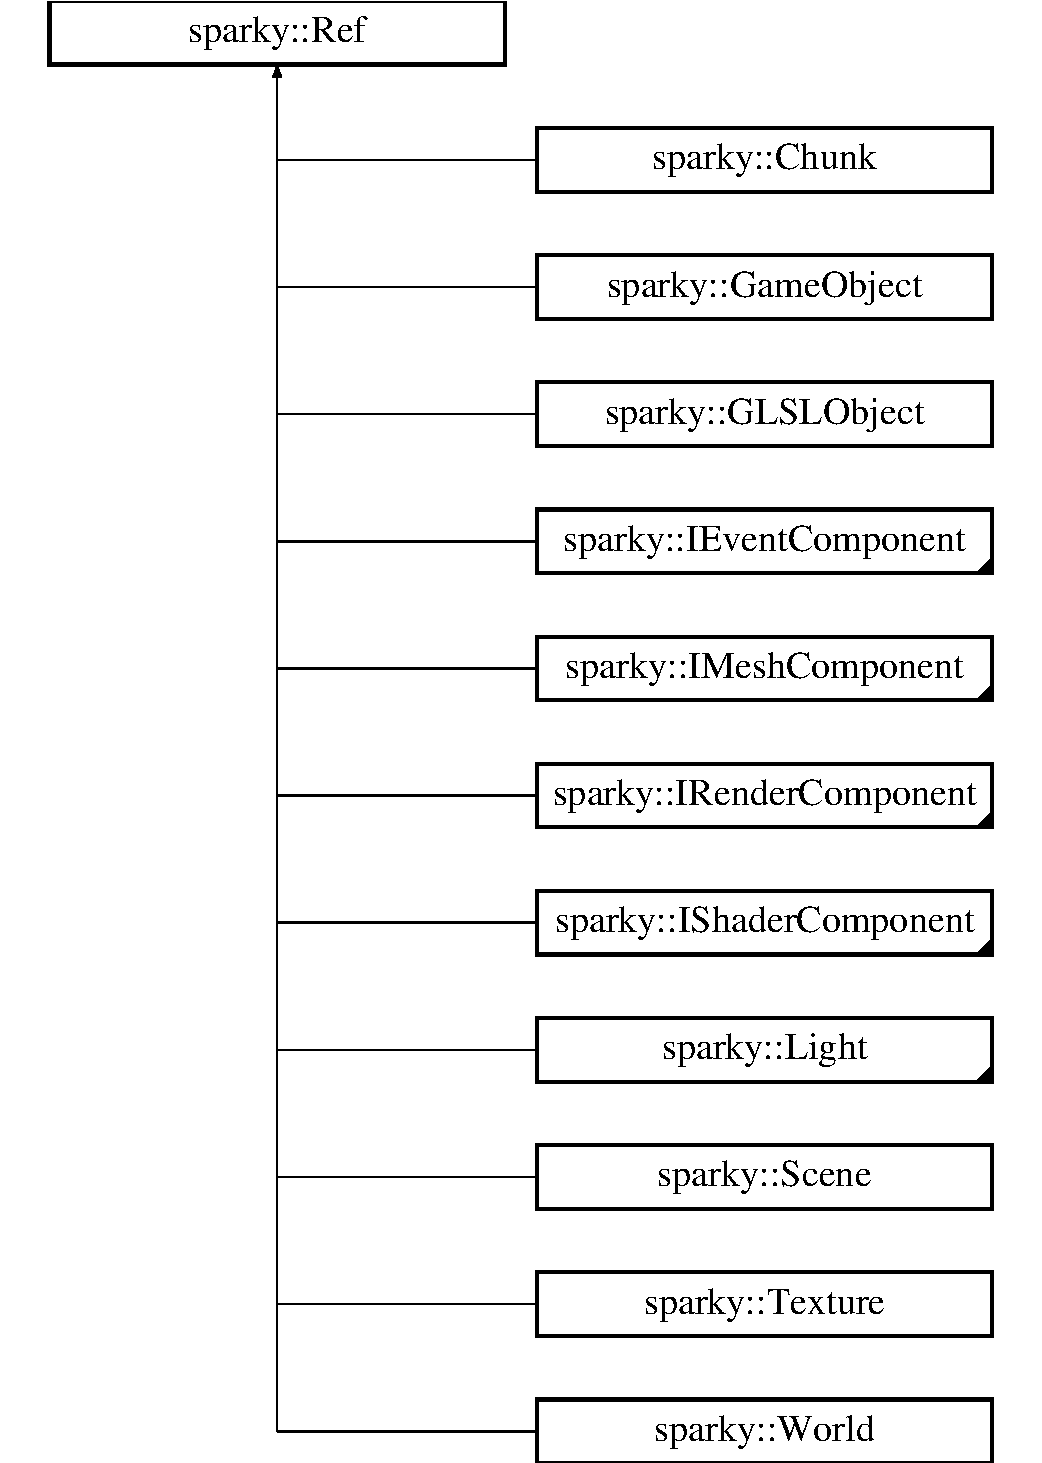
\includegraphics[height=12.000000cm]{classsparky_1_1_ref}
\end{center}
\end{figure}
\subsection*{Public Member Functions}
\begin{DoxyCompactItemize}
\item 
\hyperlink{classsparky_1_1_ref_a0947962689474dc06248f52e62022729}{Ref} (void)
\begin{DoxyCompactList}\small\item\em Constructs a \hyperlink{classsparky_1_1_ref}{Ref} object instance. \end{DoxyCompactList}\item 
virtual \hyperlink{classsparky_1_1_ref_ac1f745dbc70be6aa1550d08bb5d74d27}{$\sim$\+Ref} (void)=default
\begin{DoxyCompactList}\small\item\em Destructs a \hyperlink{classsparky_1_1_ref}{Ref} object instance. \end{DoxyCompactList}\item 
unsigned int \hyperlink{classsparky_1_1_ref_a25f72de3eab90cc4cd17d90a2762ceb8}{get\+Ref\+Count} (void) const 
\begin{DoxyCompactList}\small\item\em Gets the current reference count of the \hyperlink{classsparky_1_1_ref}{Ref}. \end{DoxyCompactList}\item 
void \hyperlink{classsparky_1_1_ref_aeeb606836c315aa3b8a2254e23eb0899}{add\+Ref} (void)
\begin{DoxyCompactList}\small\item\em Adds a reference count to the \hyperlink{classsparky_1_1_ref}{Ref}. \end{DoxyCompactList}\item 
void \hyperlink{classsparky_1_1_ref_acb1878708d20ec8051a8182a83c4a370}{remove\+Ref} (void)
\begin{DoxyCompactList}\small\item\em Removes a reference count from the \hyperlink{classsparky_1_1_ref}{Ref}. \end{DoxyCompactList}\end{DoxyCompactItemize}
\subsection*{Static Public Member Functions}
\begin{DoxyCompactItemize}
\item 
{\footnotesize template$<$typename T $>$ }\\static void \hyperlink{classsparky_1_1_ref_a3234294a7cd7ca2c0da66c76234f4b59}{release} (T \&ref)
\begin{DoxyCompactList}\small\item\em Error-\/checking and referencing decrementing of \hyperlink{classsparky_1_1_ref}{Ref} objects. \end{DoxyCompactList}\end{DoxyCompactItemize}


\subsection{Detailed Description}
\hyperlink{classsparky_1_1_ref}{sparky\+::\+Ref} is a referenced counted class which all dynamically allocated resources within the engine will inherit from. This is Sparky\textquotesingle{}s inbuilt methodology for providing basic Garbage Collection.

\hyperlink{classsparky_1_1_ref}{sparky\+::\+Ref} is commonly not used by itself, it is typically inherited from and provides its uses for subsequent child classes. However the user can use the base \hyperlink{classsparky_1_1_ref}{Ref} class if they so choose. Below is an example on how to use the functionality of the \hyperlink{classsparky_1_1_ref}{Ref} class.

Usage example\+: 
\begin{DoxyCode}
\textcolor{comment}{// Create an Ref and retain it.}
\hyperlink{classsparky_1_1_ref}{sparky::Ref}* pObject = \textcolor{keyword}{new} \hyperlink{classsparky_1_1_ref}{sparky::Ref}();
pObject->\hyperlink{classsparky_1_1_ref_aeeb606836c315aa3b8a2254e23eb0899}{addRef}();

\textcolor{comment}{// Use the object.}
\textcolor{comment}{// PoolManager is flushed}
\hyperlink{classsparky_1_1_singleton_a8e56848cf24e5f4cdcd493c64d576f10}{PoolManager::getInstance}().\hyperlink{classsparky_1_1_pool_manager_a32fb836cefbcd22763895259779eea65}{flush}();
\textcolor{comment}{// Release upon end-of-use. The counter will be decremented and }
\textcolor{comment}{// the object will be subsequently destroyed.}
\hyperlink{classsparky_1_1_ref_a3234294a7cd7ca2c0da66c76234f4b59}{Ref::release}(pObject);
\end{DoxyCode}
 

\subsection{Constructor \& Destructor Documentation}
\index{sparky\+::\+Ref@{sparky\+::\+Ref}!Ref@{Ref}}
\index{Ref@{Ref}!sparky\+::\+Ref@{sparky\+::\+Ref}}
\subsubsection[{\texorpdfstring{Ref(void)}{Ref(void)}}]{\setlength{\rightskip}{0pt plus 5cm}sparky\+::\+Ref\+::\+Ref (
\begin{DoxyParamCaption}
\item[{void}]{}
\end{DoxyParamCaption}
)\hspace{0.3cm}{\ttfamily [explicit]}}\hypertarget{classsparky_1_1_ref_a0947962689474dc06248f52e62022729}{}\label{classsparky_1_1_ref_a0947962689474dc06248f52e62022729}


Constructs a \hyperlink{classsparky_1_1_ref}{Ref} object instance. 

This default constructor initialises the \hyperlink{classsparky_1_1_ref}{Ref} and sets the reference count to one. Upon construction the object is added to the \hyperlink{classsparky_1_1_pool_manager}{Pool\+Manager}. At the end of the current frame the pool is emptied and cleared and all \hyperlink{classsparky_1_1_ref}{Ref} objects within the list have their references decremented. If the count is equal to 0, the \hyperlink{classsparky_1_1_ref}{Ref} object is deleted. \index{sparky\+::\+Ref@{sparky\+::\+Ref}!````~Ref@{$\sim$\+Ref}}
\index{````~Ref@{$\sim$\+Ref}!sparky\+::\+Ref@{sparky\+::\+Ref}}
\subsubsection[{\texorpdfstring{$\sim$\+Ref(void)=default}{~Ref(void)=default}}]{\setlength{\rightskip}{0pt plus 5cm}virtual sparky\+::\+Ref\+::$\sim$\+Ref (
\begin{DoxyParamCaption}
\item[{void}]{}
\end{DoxyParamCaption}
)\hspace{0.3cm}{\ttfamily [virtual]}, {\ttfamily [default]}}\hypertarget{classsparky_1_1_ref_ac1f745dbc70be6aa1550d08bb5d74d27}{}\label{classsparky_1_1_ref_ac1f745dbc70be6aa1550d08bb5d74d27}


Destructs a \hyperlink{classsparky_1_1_ref}{Ref} object instance. 

The \hyperlink{classsparky_1_1_ref}{Ref} only provides a default destructor as the objects inheriting from this object will define their destruction, \hyperlink{classsparky_1_1_ref}{Ref} itself contains no dynamically allocated memory. 

\subsection{Member Function Documentation}
\index{sparky\+::\+Ref@{sparky\+::\+Ref}!add\+Ref@{add\+Ref}}
\index{add\+Ref@{add\+Ref}!sparky\+::\+Ref@{sparky\+::\+Ref}}
\subsubsection[{\texorpdfstring{add\+Ref(void)}{addRef(void)}}]{\setlength{\rightskip}{0pt plus 5cm}void sparky\+::\+Ref\+::add\+Ref (
\begin{DoxyParamCaption}
\item[{void}]{}
\end{DoxyParamCaption}
)}\hypertarget{classsparky_1_1_ref_aeeb606836c315aa3b8a2254e23eb0899}{}\label{classsparky_1_1_ref_aeeb606836c315aa3b8a2254e23eb0899}


Adds a reference count to the \hyperlink{classsparky_1_1_ref}{Ref}. 

Whenever an \hyperlink{classsparky_1_1_ref}{Ref} is referenced within another class and needs to live throughout that instances lifetime, the \hyperlink{classsparky_1_1_ref}{Ref} in questions reference should be incremented in order to prevent automatic de-\/allocation. \index{sparky\+::\+Ref@{sparky\+::\+Ref}!get\+Ref\+Count@{get\+Ref\+Count}}
\index{get\+Ref\+Count@{get\+Ref\+Count}!sparky\+::\+Ref@{sparky\+::\+Ref}}
\subsubsection[{\texorpdfstring{get\+Ref\+Count(void) const }{getRefCount(void) const }}]{\setlength{\rightskip}{0pt plus 5cm}unsigned int sparky\+::\+Ref\+::get\+Ref\+Count (
\begin{DoxyParamCaption}
\item[{void}]{}
\end{DoxyParamCaption}
) const}\hypertarget{classsparky_1_1_ref_a25f72de3eab90cc4cd17d90a2762ceb8}{}\label{classsparky_1_1_ref_a25f72de3eab90cc4cd17d90a2762ceb8}


Gets the current reference count of the \hyperlink{classsparky_1_1_ref}{Ref}. 

The reference count refers to the amount of times that this current \hyperlink{classsparky_1_1_ref}{Ref} has been referenced by other classes, this is to ensure that objects can be shared between many instances without any one instance being responsible for the \hyperlink{classsparky_1_1_ref}{Ref} desctruction. This means that less memory has to be utilised within the application.


\begin{DoxyRetVals}{Return values}
{\em references} & The amount of references to the \hyperlink{classsparky_1_1_ref}{Ref}. \\
\hline
\end{DoxyRetVals}
\index{sparky\+::\+Ref@{sparky\+::\+Ref}!release@{release}}
\index{release@{release}!sparky\+::\+Ref@{sparky\+::\+Ref}}
\subsubsection[{\texorpdfstring{release(\+T \&ref)}{release(T &ref)}}]{\setlength{\rightskip}{0pt plus 5cm}template$<$typename T $>$ void sparky\+::\+Ref\+::release (
\begin{DoxyParamCaption}
\item[{T \&}]{ref}
\end{DoxyParamCaption}
)\hspace{0.3cm}{\ttfamily [static]}}\hypertarget{classsparky_1_1_ref_a3234294a7cd7ca2c0da66c76234f4b59}{}\label{classsparky_1_1_ref_a3234294a7cd7ca2c0da66c76234f4b59}


Error-\/checking and referencing decrementing of \hyperlink{classsparky_1_1_ref}{Ref} objects. 

A convenience method for checking whether the current reference is valid. if the \hyperlink{classsparky_1_1_ref}{Ref} is value, the \hyperlink{classsparky_1_1_ref}{Ref} reference count is decremented and upon reaching 0 references, the \hyperlink{classsparky_1_1_ref}{Ref} is automatically de-\/allocated and set to null.


\begin{DoxyParams}{Parameters}
{\em ref} & The \hyperlink{classsparky_1_1_ref}{Ref} to decrement and de-\/allocate. \\
\hline
\end{DoxyParams}
\index{sparky\+::\+Ref@{sparky\+::\+Ref}!remove\+Ref@{remove\+Ref}}
\index{remove\+Ref@{remove\+Ref}!sparky\+::\+Ref@{sparky\+::\+Ref}}
\subsubsection[{\texorpdfstring{remove\+Ref(void)}{removeRef(void)}}]{\setlength{\rightskip}{0pt plus 5cm}void sparky\+::\+Ref\+::remove\+Ref (
\begin{DoxyParamCaption}
\item[{void}]{}
\end{DoxyParamCaption}
)}\hypertarget{classsparky_1_1_ref_acb1878708d20ec8051a8182a83c4a370}{}\label{classsparky_1_1_ref_acb1878708d20ec8051a8182a83c4a370}


Removes a reference count from the \hyperlink{classsparky_1_1_ref}{Ref}. 

When a call no longer needs to retain a reference to the \hyperlink{classsparky_1_1_ref}{Ref}, the reference counter should be decremented. 

The documentation for this class was generated from the following file\+:\begin{DoxyCompactItemize}
\item 
C\+:/\+Users/\+Ben/\+Documents/repos/sparky/include/sparky/core/ref.\+hpp\end{DoxyCompactItemize}

\hypertarget{classsparky_1_1_resource_holder}{}\section{sparky\+:\+:Resource\+Holder$<$ T $>$ Class Template Reference}
\label{classsparky_1_1_resource_holder}\index{sparky\+::\+Resource\+Holder$<$ T $>$@{sparky\+::\+Resource\+Holder$<$ T $>$}}


{\ttfamily \#include $<$resourceholder.\+hpp$>$}

\subsection*{Public Member Functions}
\begin{DoxyCompactItemize}
\item 
\hyperlink{classsparky_1_1_resource_holder_ab6c7da674e75bb5fdddb9f093540d84c}{Resource\+Holder} (void)
\begin{DoxyCompactList}\small\item\em Default construction of the \hyperlink{classsparky_1_1_resource_holder}{Resource\+Holder} object. \end{DoxyCompactList}\item 
virtual \hyperlink{classsparky_1_1_resource_holder_a59e8662ddb4e6385357433b28d8d3f20}{$\sim$\+Resource\+Holder} (void)
\begin{DoxyCompactList}\small\item\em Destruction of the \hyperlink{classsparky_1_1_resource_holder}{Resource\+Holder} object. \end{DoxyCompactList}\item 
T $\ast$ \hyperlink{classsparky_1_1_resource_holder_a7eba84d365632c96abdb4f88101b0942}{get} (const \hyperlink{classsparky_1_1_string}{String} \&name) const 
\begin{DoxyCompactList}\small\item\em Retrieves a resource (by name) from the \hyperlink{classsparky_1_1_resource_holder}{Resource\+Holder}. \end{DoxyCompactList}\item 
void \hyperlink{classsparky_1_1_resource_holder_a29eeacabc85f240b3a44e677d659fcf3}{add} (const \hyperlink{classsparky_1_1_string}{String} \&name, T $\ast$p\+Resource)
\begin{DoxyCompactList}\small\item\em Adds a resource to the map with an associated \hyperlink{classsparky_1_1_string}{String} key. \end{DoxyCompactList}\item 
void \hyperlink{classsparky_1_1_resource_holder_a7b5efe2ea2ca622774bcb171d34199ad}{remove} (const \hyperlink{classsparky_1_1_string}{String} \&name)
\begin{DoxyCompactList}\small\item\em Removes a resource from the \hyperlink{classsparky_1_1_resource_holder}{Resource\+Holder} object. \end{DoxyCompactList}\end{DoxyCompactItemize}


\subsection{Detailed Description}
\subsubsection*{template$<$typename T$>$\\*
class sparky\+::\+Resource\+Holder$<$ T $>$}

\hyperlink{classsparky_1_1_resource_holder}{sparky\+::\+Resource\+Holder} is a parent class resource storage object. It is used to store assets that will be commonly used throughout the application, such as Shaders and Textures.

The Resource Holder prevents duplication of objects, so that the engine is as efficient as possible during runtime. The \hyperlink{classsparky_1_1_resource_holder}{Resource\+Holder} can store all assets used by the application before starting by adding them when the application is first started.

Objects within the \hyperlink{classsparky_1_1_resource_holder}{Resource\+Holder} must inherit from \hyperlink{classsparky_1_1_ref}{sparky\+::\+Ref} to comply with Sparky\textquotesingle{}s memory management scheme. Below is pseudo-\/code example.

Usage example\+: 
\begin{DoxyCode}
\textcolor{comment}{// Create a sample user type. (Must inherit from Ref).}
\textcolor{keyword}{struct }Type : \textcolor{keyword}{public} Ref
\{
    \textcolor{keywordtype}{int} x;
\}

\textcolor{comment}{// Create a resource holder to hold the different types.}
\hyperlink{classsparky_1_1_resource_holder}{sparky::ResourceHolder<Type>} holder;

\textcolor{comment}{// Add a type to the holder}
holder.\hyperlink{classsparky_1_1_resource_holder_a29eeacabc85f240b3a44e677d659fcf3}{add}(\textcolor{stringliteral}{"Type"}, \textcolor{keyword}{new} Type());

\textcolor{comment}{// Retrieve a object from the holder and print it to the console.}
std::cout << holder.\hyperlink{classsparky_1_1_resource_holder_a7eba84d365632c96abdb4f88101b0942}{get}(\textcolor{stringliteral}{"Type"}).x << std::endl;
\end{DoxyCode}
 

\subsection{Constructor \& Destructor Documentation}
\index{sparky\+::\+Resource\+Holder@{sparky\+::\+Resource\+Holder}!Resource\+Holder@{Resource\+Holder}}
\index{Resource\+Holder@{Resource\+Holder}!sparky\+::\+Resource\+Holder@{sparky\+::\+Resource\+Holder}}
\subsubsection[{\texorpdfstring{Resource\+Holder(void)}{ResourceHolder(void)}}]{\setlength{\rightskip}{0pt plus 5cm}template$<$typename T$>$ {\bf sparky\+::\+Resource\+Holder}$<$ T $>$\+::{\bf Resource\+Holder} (
\begin{DoxyParamCaption}
\item[{void}]{}
\end{DoxyParamCaption}
)\hspace{0.3cm}{\ttfamily [explicit]}}\hypertarget{classsparky_1_1_resource_holder_ab6c7da674e75bb5fdddb9f093540d84c}{}\label{classsparky_1_1_resource_holder_ab6c7da674e75bb5fdddb9f093540d84c}


Default construction of the \hyperlink{classsparky_1_1_resource_holder}{Resource\+Holder} object. 

The default construction of the \hyperlink{classsparky_1_1_resource_holder}{Resource\+Holder} only sets the member variables to default values. \index{sparky\+::\+Resource\+Holder@{sparky\+::\+Resource\+Holder}!````~Resource\+Holder@{$\sim$\+Resource\+Holder}}
\index{````~Resource\+Holder@{$\sim$\+Resource\+Holder}!sparky\+::\+Resource\+Holder@{sparky\+::\+Resource\+Holder}}
\subsubsection[{\texorpdfstring{$\sim$\+Resource\+Holder(void)}{~ResourceHolder(void)}}]{\setlength{\rightskip}{0pt plus 5cm}template$<$typename T$>$ virtual {\bf sparky\+::\+Resource\+Holder}$<$ T $>$\+::$\sim${\bf Resource\+Holder} (
\begin{DoxyParamCaption}
\item[{void}]{}
\end{DoxyParamCaption}
)\hspace{0.3cm}{\ttfamily [virtual]}}\hypertarget{classsparky_1_1_resource_holder_a59e8662ddb4e6385357433b28d8d3f20}{}\label{classsparky_1_1_resource_holder_a59e8662ddb4e6385357433b28d8d3f20}


Destruction of the \hyperlink{classsparky_1_1_resource_holder}{Resource\+Holder} object. 

The destruction of the \hyperlink{classsparky_1_1_resource_holder}{Resource\+Holder} will release the resources being retained by the Holder object. 

\subsection{Member Function Documentation}
\index{sparky\+::\+Resource\+Holder@{sparky\+::\+Resource\+Holder}!add@{add}}
\index{add@{add}!sparky\+::\+Resource\+Holder@{sparky\+::\+Resource\+Holder}}
\subsubsection[{\texorpdfstring{add(const String \&name, T $\ast$p\+Resource)}{add(const String &name, T *pResource)}}]{\setlength{\rightskip}{0pt plus 5cm}template$<$typename T$>$ void {\bf sparky\+::\+Resource\+Holder}$<$ T $>$\+::add (
\begin{DoxyParamCaption}
\item[{const {\bf String} \&}]{name, }
\item[{T $\ast$}]{p\+Resource}
\end{DoxyParamCaption}
)}\hypertarget{classsparky_1_1_resource_holder_a29eeacabc85f240b3a44e677d659fcf3}{}\label{classsparky_1_1_resource_holder_a29eeacabc85f240b3a44e677d659fcf3}


Adds a resource to the map with an associated \hyperlink{classsparky_1_1_string}{String} key. 

When a resource is added to the \hyperlink{classsparky_1_1_resource_holder}{Resource\+Holder} object, it checks to make sure that no objects have the same key. If the key is not found the resource parameter is retained and added as a pair to the resource map.


\begin{DoxyParams}{Parameters}
{\em name} & The desginated key of the resource. \\
\hline
{\em p\+Resource} & The resource to add to the map. \\
\hline
\end{DoxyParams}
\index{sparky\+::\+Resource\+Holder@{sparky\+::\+Resource\+Holder}!get@{get}}
\index{get@{get}!sparky\+::\+Resource\+Holder@{sparky\+::\+Resource\+Holder}}
\subsubsection[{\texorpdfstring{get(const String \&name) const }{get(const String &name) const }}]{\setlength{\rightskip}{0pt plus 5cm}template$<$typename T$>$ T$\ast$ {\bf sparky\+::\+Resource\+Holder}$<$ T $>$\+::get (
\begin{DoxyParamCaption}
\item[{const {\bf String} \&}]{name}
\end{DoxyParamCaption}
) const}\hypertarget{classsparky_1_1_resource_holder_a7eba84d365632c96abdb4f88101b0942}{}\label{classsparky_1_1_resource_holder_a7eba84d365632c96abdb4f88101b0942}


Retrieves a resource (by name) from the \hyperlink{classsparky_1_1_resource_holder}{Resource\+Holder}. 

The map is search by name from the current resources and retrieves the value which matches the parameter name. If the resource is not found, a warning message is printed to the console window and the method will return a null pointer.


\begin{DoxyParams}{Parameters}
{\em name} & The name of the resource to retrieve.\\
\hline
\end{DoxyParams}

\begin{DoxyRetVals}{Return values}
{\em T} & The resource associated with the name. If the resource is not found, null pointer is returned. \\
\hline
\end{DoxyRetVals}
\index{sparky\+::\+Resource\+Holder@{sparky\+::\+Resource\+Holder}!remove@{remove}}
\index{remove@{remove}!sparky\+::\+Resource\+Holder@{sparky\+::\+Resource\+Holder}}
\subsubsection[{\texorpdfstring{remove(const String \&name)}{remove(const String &name)}}]{\setlength{\rightskip}{0pt plus 5cm}template$<$typename T$>$ void {\bf sparky\+::\+Resource\+Holder}$<$ T $>$\+::remove (
\begin{DoxyParamCaption}
\item[{const {\bf String} \&}]{name}
\end{DoxyParamCaption}
)}\hypertarget{classsparky_1_1_resource_holder_a7b5efe2ea2ca622774bcb171d34199ad}{}\label{classsparky_1_1_resource_holder_a7b5efe2ea2ca622774bcb171d34199ad}


Removes a resource from the \hyperlink{classsparky_1_1_resource_holder}{Resource\+Holder} object. 

When an object is removed, the map is searched to make sure that this object is in the Holder. If it is the object is erased from storage and released. When all other objects are no longer referencing this resource, the object will be de-\/allocated.


\begin{DoxyParams}{Parameters}
{\em name} & The key of the resource to remove. \\
\hline
\end{DoxyParams}


The documentation for this class was generated from the following file\+:\begin{DoxyCompactItemize}
\item 
C\+:/\+Users/\+Ben/\+Documents/repos/sparky/include/sparky/core/resourceholder.\+hpp\end{DoxyCompactItemize}

\hypertarget{classsparky_1_1_resource_manager}{}\section{sparky\+:\+:Resource\+Manager Class Reference}
\label{classsparky_1_1_resource_manager}\index{sparky\+::\+Resource\+Manager@{sparky\+::\+Resource\+Manager}}


{\ttfamily \#include $<$resourcemanager.\+hpp$>$}

Inheritance diagram for sparky\+:\+:Resource\+Manager\+:\begin{figure}[H]
\begin{center}
\leavevmode
\includegraphics[height=2.000000cm]{classsparky_1_1_resource_manager}
\end{center}
\end{figure}
\subsection*{Public Member Functions}
\begin{DoxyCompactItemize}
\item 
\hyperlink{classsparky_1_1_resource_manager_a19e493845527b32781864921284a02bb}{$\sim$\+Resource\+Manager} (void)=default\hypertarget{classsparky_1_1_resource_manager_a19e493845527b32781864921284a02bb}{}\label{classsparky_1_1_resource_manager_a19e493845527b32781864921284a02bb}

\begin{DoxyCompactList}\small\item\em Default destruction of the \hyperlink{classsparky_1_1_resource_manager}{Resource\+Manager} singleton. \end{DoxyCompactList}\item 
{\footnotesize template$<$typename T  = I\+Shader\+Component$>$ }\\T $\ast$ \hyperlink{classsparky_1_1_resource_manager_a8d48e497254410edf301df3d08248520}{get\+Shader} (const \hyperlink{classsparky_1_1_string}{String} \&name) const 
\begin{DoxyCompactList}\small\item\em Retrieves a shader from the \hyperlink{classsparky_1_1_resource_holder}{Resource\+Holder} lists. \end{DoxyCompactList}\item 
void \hyperlink{classsparky_1_1_resource_manager_aadcd7a39dafd4d1d7dcfc8c2cc2735d2}{add\+Shader} (const \hyperlink{classsparky_1_1_string}{String} \&name, \hyperlink{classsparky_1_1_i_shader_component}{I\+Shader\+Component} $\ast$p\+Shader)
\begin{DoxyCompactList}\small\item\em Adds a shader to the \hyperlink{classsparky_1_1_resource_holder}{Resource\+Holder} lists. \end{DoxyCompactList}\item 
void \hyperlink{classsparky_1_1_resource_manager_a7bb2b24c2f74a4ee23d00cf11f0fea95}{remove\+Shader} (const \hyperlink{classsparky_1_1_string}{String} \&name)
\begin{DoxyCompactList}\small\item\em Removes a shader from the \hyperlink{classsparky_1_1_resource_holder}{Resource\+Holder} lists. \end{DoxyCompactList}\end{DoxyCompactItemize}
\subsection*{Friends}
\begin{DoxyCompactItemize}
\item 
class {\bfseries Singleton$<$ Resource\+Manager $>$}\hypertarget{classsparky_1_1_resource_manager_a8cc0c523af7e6e454ed0f273b5f18e4a}{}\label{classsparky_1_1_resource_manager_a8cc0c523af7e6e454ed0f273b5f18e4a}

\end{DoxyCompactItemize}
\subsection*{Additional Inherited Members}


\subsection{Detailed Description}
\hyperlink{classsparky_1_1_resource_manager}{sparky\+::\+Resource\+Manager} is a singleton class which retains commonly used assets and shaders used throughout the engine for quick retrieval and use. When the Resource Manager is utilised, external sources only have to be loaded into the engine once, which saves additional time and memory.

Which becomes especially helpful when utilising different shaders in different files, the shaders can be used without the use of additional functionality or parameters. Below is a code example.

Usage example\+: 
\begin{DoxyCode}
\textcolor{comment}{// Add a Basic shader to the Resource Manager.}
\hyperlink{classsparky_1_1_singleton_a8e56848cf24e5f4cdcd493c64d576f10}{sparky::ResourceManager::getInstance}().
      \hyperlink{classsparky_1_1_resource_manager_aadcd7a39dafd4d1d7dcfc8c2cc2735d2}{addShader}(\textcolor{stringliteral}{"basic"}, \textcolor{keyword}{new} \hyperlink{classsparky_1_1_directional_shader}{sparky::DirectionalShader}());

\textcolor{comment}{// Get a local reference of the shader for use.}
\hyperlink{classsparky_1_1_directional_shader}{sparky::DirectionalShader}* pShader = 
      \hyperlink{classsparky_1_1_singleton_a8e56848cf24e5f4cdcd493c64d576f10}{sparky::ResourceManager::getInstance}().
      \hyperlink{classsparky_1_1_resource_manager_a8d48e497254410edf301df3d08248520}{getShader}<DirectionalShader>(\textcolor{stringliteral}{"directional"});

\textcolor{comment}{// Bind the shader for use.}
pShader->\hyperlink{classsparky_1_1_i_shader_component_a6ed7ff5dbe96d0fb5bc8f3e53e110e1a}{bind}();
\end{DoxyCode}
 

\subsection{Member Function Documentation}
\index{sparky\+::\+Resource\+Manager@{sparky\+::\+Resource\+Manager}!add\+Shader@{add\+Shader}}
\index{add\+Shader@{add\+Shader}!sparky\+::\+Resource\+Manager@{sparky\+::\+Resource\+Manager}}
\subsubsection[{\texorpdfstring{add\+Shader(const String \&name, I\+Shader\+Component $\ast$p\+Shader)}{addShader(const String &name, IShaderComponent *pShader)}}]{\setlength{\rightskip}{0pt plus 5cm}void sparky\+::\+Resource\+Manager\+::add\+Shader (
\begin{DoxyParamCaption}
\item[{const {\bf String} \&}]{name, }
\item[{{\bf I\+Shader\+Component} $\ast$}]{p\+Shader}
\end{DoxyParamCaption}
)}\hypertarget{classsparky_1_1_resource_manager_aadcd7a39dafd4d1d7dcfc8c2cc2735d2}{}\label{classsparky_1_1_resource_manager_aadcd7a39dafd4d1d7dcfc8c2cc2735d2}


Adds a shader to the \hyperlink{classsparky_1_1_resource_holder}{Resource\+Holder} lists. 

Adds a shader to the \hyperlink{classsparky_1_1_resource_holder}{Resource\+Holder} lists. If a shader has already been added that has an identical name, then the shader is not added to the list and a warning message is produced.


\begin{DoxyParams}{Parameters}
{\em name} & The keyword name associated with this shader. \\
\hline
{\em p\+Shader} & The shader to add to the \hyperlink{classsparky_1_1_resource_holder}{Resource\+Holder}. \\
\hline
\end{DoxyParams}
\index{sparky\+::\+Resource\+Manager@{sparky\+::\+Resource\+Manager}!get\+Shader@{get\+Shader}}
\index{get\+Shader@{get\+Shader}!sparky\+::\+Resource\+Manager@{sparky\+::\+Resource\+Manager}}
\subsubsection[{\texorpdfstring{get\+Shader(const String \&name) const }{getShader(const String &name) const }}]{\setlength{\rightskip}{0pt plus 5cm}template$<$typename T $>$ T $\ast$ sparky\+::\+Resource\+Manager\+::get\+Shader (
\begin{DoxyParamCaption}
\item[{const {\bf String} \&}]{name}
\end{DoxyParamCaption}
) const}\hypertarget{classsparky_1_1_resource_manager_a8d48e497254410edf301df3d08248520}{}\label{classsparky_1_1_resource_manager_a8d48e497254410edf301df3d08248520}


Retrieves a shader from the \hyperlink{classsparky_1_1_resource_holder}{Resource\+Holder} lists. 

Searches the \hyperlink{classsparky_1_1_resource_holder}{Resource\+Holder} of shaders for the shader with the specified name. If the shader is not found, an error message is produced and nullptr is returned.


\begin{DoxyParams}{Parameters}
{\em name} & The name of the shader to retrieve. \\
\hline
\end{DoxyParams}
\index{sparky\+::\+Resource\+Manager@{sparky\+::\+Resource\+Manager}!remove\+Shader@{remove\+Shader}}
\index{remove\+Shader@{remove\+Shader}!sparky\+::\+Resource\+Manager@{sparky\+::\+Resource\+Manager}}
\subsubsection[{\texorpdfstring{remove\+Shader(const String \&name)}{removeShader(const String &name)}}]{\setlength{\rightskip}{0pt plus 5cm}void sparky\+::\+Resource\+Manager\+::remove\+Shader (
\begin{DoxyParamCaption}
\item[{const {\bf String} \&}]{name}
\end{DoxyParamCaption}
)}\hypertarget{classsparky_1_1_resource_manager_a7bb2b24c2f74a4ee23d00cf11f0fea95}{}\label{classsparky_1_1_resource_manager_a7bb2b24c2f74a4ee23d00cf11f0fea95}


Removes a shader from the \hyperlink{classsparky_1_1_resource_holder}{Resource\+Holder} lists. 

Removes a shader by name from the \hyperlink{classsparky_1_1_resource_holder}{Resource\+Holder} lists. If the shader is not found, a warning message is printed and the lists are left untouched.


\begin{DoxyParams}{Parameters}
{\em name} & The name of the shader object to remove. \\
\hline
\end{DoxyParams}


The documentation for this class was generated from the following file\+:\begin{DoxyCompactItemize}
\item 
C\+:/\+Users/\+Ben/\+Documents/repos/sparky/include/sparky/core/resourcemanager.\+hpp\end{DoxyCompactItemize}

\hypertarget{classsparky_1_1_scene}{}\section{sparky\+:\+:Scene Class Reference}
\label{classsparky_1_1_scene}\index{sparky\+::\+Scene@{sparky\+::\+Scene}}


{\ttfamily \#include $<$scene.\+hpp$>$}

Inheritance diagram for sparky\+:\+:Scene\+:\begin{figure}[H]
\begin{center}
\leavevmode
\includegraphics[height=2.000000cm]{classsparky_1_1_scene}
\end{center}
\end{figure}
\subsection*{Public Member Functions}
\begin{DoxyCompactItemize}
\item 
\hyperlink{classsparky_1_1_scene_a39f382a2e4f39ef9585e282bcd7bd8fc}{Scene} (void)\hypertarget{classsparky_1_1_scene_a39f382a2e4f39ef9585e282bcd7bd8fc}{}\label{classsparky_1_1_scene_a39f382a2e4f39ef9585e282bcd7bd8fc}

\begin{DoxyCompactList}\small\item\em Default constructor for the \hyperlink{classsparky_1_1_scene}{Scene} object class. \end{DoxyCompactList}\item 
virtual \hyperlink{classsparky_1_1_scene_afac76d9ed35f5a3abf24d48ac2c7c79c}{$\sim$\+Scene} (void)=default\hypertarget{classsparky_1_1_scene_afac76d9ed35f5a3abf24d48ac2c7c79c}{}\label{classsparky_1_1_scene_afac76d9ed35f5a3abf24d48ac2c7c79c}

\begin{DoxyCompactList}\small\item\em Destructor for the \hyperlink{classsparky_1_1_scene}{Scene} object class. \end{DoxyCompactList}\item 
virtual void \hyperlink{classsparky_1_1_scene_a108c7eab94934c57a7e92aa52d735117}{update} (void)=0
\begin{DoxyCompactList}\small\item\em Pure virtual update method for scenes. \end{DoxyCompactList}\item 
virtual void \hyperlink{classsparky_1_1_scene_ac1018bd5a77e5505e3a40a186e171aea}{render} (void)=0
\begin{DoxyCompactList}\small\item\em Pure virtual render method for scenes. \end{DoxyCompactList}\end{DoxyCompactItemize}
\subsection*{Additional Inherited Members}


\subsection{Detailed Description}
\hyperlink{classsparky_1_1_scene}{sparky\+::\+Scene} is an abstract class in which all scenes will inherit from in an application. A scene refers to a level in a game, the scenes can be pushed and popped from the Game Manager stack so that more functionality can easily be added or removed.

Below is a code example where a child class for Game has theoretically been created.

Usage example\+: 
\begin{DoxyCode}
\textcolor{comment}{// Create a new Game object.}
Game* pGame = \textcolor{keyword}{new} Game();

\textcolor{comment}{// Add the game as the first level in the application.}
\hyperlink{classsparky_1_1_singleton_a8e56848cf24e5f4cdcd493c64d576f10}{sparky::GameManager::getInstance}().pushScene(pGame);
\end{DoxyCode}
 

\subsection{Member Function Documentation}
\index{sparky\+::\+Scene@{sparky\+::\+Scene}!render@{render}}
\index{render@{render}!sparky\+::\+Scene@{sparky\+::\+Scene}}
\subsubsection[{\texorpdfstring{render(void)=0}{render(void)=0}}]{\setlength{\rightskip}{0pt plus 5cm}virtual void sparky\+::\+Scene\+::render (
\begin{DoxyParamCaption}
\item[{void}]{}
\end{DoxyParamCaption}
)\hspace{0.3cm}{\ttfamily [pure virtual]}}\hypertarget{classsparky_1_1_scene_ac1018bd5a77e5505e3a40a186e171aea}{}\label{classsparky_1_1_scene_ac1018bd5a77e5505e3a40a186e171aea}


Pure virtual render method for scenes. 

The render method will be overwritten by child classes. The rendering will be called every frame and should only contain the information to render specific objects. \index{sparky\+::\+Scene@{sparky\+::\+Scene}!update@{update}}
\index{update@{update}!sparky\+::\+Scene@{sparky\+::\+Scene}}
\subsubsection[{\texorpdfstring{update(void)=0}{update(void)=0}}]{\setlength{\rightskip}{0pt plus 5cm}virtual void sparky\+::\+Scene\+::update (
\begin{DoxyParamCaption}
\item[{void}]{}
\end{DoxyParamCaption}
)\hspace{0.3cm}{\ttfamily [pure virtual]}}\hypertarget{classsparky_1_1_scene_a108c7eab94934c57a7e92aa52d735117}{}\label{classsparky_1_1_scene_a108c7eab94934c57a7e92aa52d735117}


Pure virtual update method for scenes. 

The update method will be overwritten by child classes. The update will be called every frame and should contain all the logic and processing of the current \hyperlink{classsparky_1_1_scene}{Scene}. 

The documentation for this class was generated from the following file\+:\begin{DoxyCompactItemize}
\item 
C\+:/\+Users/\+Ben/\+Documents/repos/sparky/include/sparky/core/scene.\+hpp\end{DoxyCompactItemize}

\hypertarget{classsparky_1_1_singleton}{}\section{sparky\+:\+:Singleton$<$ T $>$ Class Template Reference}
\label{classsparky_1_1_singleton}\index{sparky\+::\+Singleton$<$ T $>$@{sparky\+::\+Singleton$<$ T $>$}}
Inheritance diagram for sparky\+:\+:Singleton$<$ T $>$\+:\begin{figure}[H]
\begin{center}
\leavevmode
\includegraphics[height=2.000000cm]{classsparky_1_1_singleton}
\end{center}
\end{figure}
\subsection*{Public Member Functions}
\begin{DoxyCompactItemize}
\item 
virtual \hyperlink{classsparky_1_1_singleton_aeefde4f7fc684d84734862f0e1d7ff5d}{$\sim$\+Singleton} (void)=default
\begin{DoxyCompactList}\small\item\em Default destruction of the \hyperlink{classsparky_1_1_singleton}{Singleton} instance. \end{DoxyCompactList}\end{DoxyCompactItemize}
\subsection*{Static Public Member Functions}
\begin{DoxyCompactItemize}
\item 
static T \& \hyperlink{classsparky_1_1_singleton_a8e56848cf24e5f4cdcd493c64d576f10}{get\+Instance} (void)
\begin{DoxyCompactList}\small\item\em Gets the instance of the \hyperlink{classsparky_1_1_singleton}{Singleton}. \end{DoxyCompactList}\end{DoxyCompactItemize}
\subsection*{Protected Member Functions}
\begin{DoxyCompactItemize}
\item 
\hyperlink{classsparky_1_1_singleton_a5ac95da4fe4b24114b1c019b1fc64893}{Singleton} (void)=default
\begin{DoxyCompactList}\small\item\em Default construction of a \hyperlink{classsparky_1_1_singleton}{Singleton} instance. \end{DoxyCompactList}\item 
\hyperlink{classsparky_1_1_singleton_ad580e39c175a8eb299d67815523aed0d}{Singleton} (const \hyperlink{classsparky_1_1_singleton}{Singleton}$<$ T $>$ \&other)=delete
\begin{DoxyCompactList}\small\item\em Deletes the copy constructor of a \hyperlink{classsparky_1_1_singleton}{Singleton}. \end{DoxyCompactList}\end{DoxyCompactItemize}


\subsection{Constructor \& Destructor Documentation}
\index{sparky\+::\+Singleton@{sparky\+::\+Singleton}!Singleton@{Singleton}}
\index{Singleton@{Singleton}!sparky\+::\+Singleton@{sparky\+::\+Singleton}}
\subsubsection[{\texorpdfstring{Singleton(void)=default}{Singleton(void)=default}}]{\setlength{\rightskip}{0pt plus 5cm}template$<$typename T$>$ {\bf sparky\+::\+Singleton}$<$ T $>$\+::{\bf Singleton} (
\begin{DoxyParamCaption}
\item[{void}]{}
\end{DoxyParamCaption}
)\hspace{0.3cm}{\ttfamily [explicit]}, {\ttfamily [protected]}, {\ttfamily [default]}}\hypertarget{classsparky_1_1_singleton_a5ac95da4fe4b24114b1c019b1fc64893}{}\label{classsparky_1_1_singleton_a5ac95da4fe4b24114b1c019b1fc64893}


Default construction of a \hyperlink{classsparky_1_1_singleton}{Singleton} instance. 

A singleton is a common design pattern which utilises the construction of a single instance throughout the programs lifetime. They can be used to provide convenient access to objects and methods, regardless of scope. The constructor is protected so that it cannot be accessed outside the parent or child\textquotesingle{}s scope. \index{sparky\+::\+Singleton@{sparky\+::\+Singleton}!Singleton@{Singleton}}
\index{Singleton@{Singleton}!sparky\+::\+Singleton@{sparky\+::\+Singleton}}
\subsubsection[{\texorpdfstring{Singleton(const Singleton$<$ T $>$ \&other)=delete}{Singleton(const Singleton< T > &other)=delete}}]{\setlength{\rightskip}{0pt plus 5cm}template$<$typename T$>$ {\bf sparky\+::\+Singleton}$<$ T $>$\+::{\bf Singleton} (
\begin{DoxyParamCaption}
\item[{const {\bf Singleton}$<$ T $>$ \&}]{other}
\end{DoxyParamCaption}
)\hspace{0.3cm}{\ttfamily [explicit]}, {\ttfamily [protected]}, {\ttfamily [delete]}}\hypertarget{classsparky_1_1_singleton_ad580e39c175a8eb299d67815523aed0d}{}\label{classsparky_1_1_singleton_ad580e39c175a8eb299d67815523aed0d}


Deletes the copy constructor of a \hyperlink{classsparky_1_1_singleton}{Singleton}. 

This will prevent the user from constructing any additional singleton\textquotesingle{}s from the information of another, which will provide undefined behaviour in the application.


\begin{DoxyParams}{Parameters}
{\em other} & The other \hyperlink{classsparky_1_1_singleton}{Singleton} object that will not be copied. \\
\hline
\end{DoxyParams}
\index{sparky\+::\+Singleton@{sparky\+::\+Singleton}!````~Singleton@{$\sim$\+Singleton}}
\index{````~Singleton@{$\sim$\+Singleton}!sparky\+::\+Singleton@{sparky\+::\+Singleton}}
\subsubsection[{\texorpdfstring{$\sim$\+Singleton(void)=default}{~Singleton(void)=default}}]{\setlength{\rightskip}{0pt plus 5cm}template$<$typename T$>$ virtual {\bf sparky\+::\+Singleton}$<$ T $>$\+::$\sim${\bf Singleton} (
\begin{DoxyParamCaption}
\item[{void}]{}
\end{DoxyParamCaption}
)\hspace{0.3cm}{\ttfamily [virtual]}, {\ttfamily [default]}}\hypertarget{classsparky_1_1_singleton_aeefde4f7fc684d84734862f0e1d7ff5d}{}\label{classsparky_1_1_singleton_aeefde4f7fc684d84734862f0e1d7ff5d}


Default destruction of the \hyperlink{classsparky_1_1_singleton}{Singleton} instance. 

The Parent class retains no information or dynamically allocated memory so does not need to destruct any objects. The destruction of objects will be overriden in it\textquotesingle{}s subsequent child classes. 

\subsection{Member Function Documentation}
\index{sparky\+::\+Singleton@{sparky\+::\+Singleton}!get\+Instance@{get\+Instance}}
\index{get\+Instance@{get\+Instance}!sparky\+::\+Singleton@{sparky\+::\+Singleton}}
\subsubsection[{\texorpdfstring{get\+Instance(void)}{getInstance(void)}}]{\setlength{\rightskip}{0pt plus 5cm}template$<$typename T$>$ static T\& {\bf sparky\+::\+Singleton}$<$ T $>$\+::get\+Instance (
\begin{DoxyParamCaption}
\item[{void}]{}
\end{DoxyParamCaption}
)\hspace{0.3cm}{\ttfamily [static]}}\hypertarget{classsparky_1_1_singleton_a8e56848cf24e5f4cdcd493c64d576f10}{}\label{classsparky_1_1_singleton_a8e56848cf24e5f4cdcd493c64d576f10}


Gets the instance of the \hyperlink{classsparky_1_1_singleton}{Singleton}. 

This provides access to the functionality of the \hyperlink{classsparky_1_1_singleton}{Singleton} object. As the \hyperlink{classsparky_1_1_singleton}{Singleton} can only be constructed within its own scope, you cannot access its methods without utilising the static instance of the class.


\begin{DoxyRetVals}{Return values}
{\em T\&} & The static instance of this \hyperlink{classsparky_1_1_singleton}{Singleton} object. \\
\hline
\end{DoxyRetVals}


The documentation for this class was generated from the following file\+:\begin{DoxyCompactItemize}
\item 
C\+:/\+Users/\+Ben/\+Documents/repos/sparky/include/sparky/utils/singleton.\+hpp\end{DoxyCompactItemize}

\hypertarget{classsparky_1_1_singleton_3_01_t_01_4}{}\section{sparky\+:\+:Singleton$<$ T $>$ Class Reference}
\label{classsparky_1_1_singleton_3_01_t_01_4}\index{sparky\+::\+Singleton$<$ T $>$@{sparky\+::\+Singleton$<$ T $>$}}


{\ttfamily \#include $<$singleton.\+hpp$>$}



\subsection{Detailed Description}
\hyperlink{classsparky_1_1_singleton_3_01_t_01_4}{sparky\+::\+Singleton$<$\+T$>$} is a templated base class which provides the basic implementation of a \hyperlink{classsparky_1_1_singleton}{Singleton} design pattern.

All other \hyperlink{classsparky_1_1_singleton}{Singleton}\textquotesingle{}s within the engine which provide additional behaviour will inherit from this object. The user can also create additional Singletons by inheriting from this base class.

Although you would never use this base class as-\/is. Below is a basic example of it\textquotesingle{}s uses.

Usage example\+: 
\begin{DoxyCode}
\textcolor{comment}{// Store an int Singleton in a local variable.}
Singleton<int> s = \hyperlink{classsparky_1_1_singleton_a8e56848cf24e5f4cdcd493c64d576f10}{Singleton<int>::getInstance}();
\end{DoxyCode}
 

The documentation for this class was generated from the following file\+:\begin{DoxyCompactItemize}
\item 
C\+:/\+Users/\+Ben/\+Documents/repos/sparky/include/sparky/utils/singleton.\+hpp\end{DoxyCompactItemize}

\hypertarget{structsparky_1_1_s_p_a_r_k_y___b_a_s_e___l_i_g_h_t___d_e_s_c}{}\section{sparky\+:\+:S\+P\+A\+R\+K\+Y\+\_\+\+B\+A\+S\+E\+\_\+\+L\+I\+G\+H\+T\+\_\+\+D\+E\+SC Struct Reference}
\label{structsparky_1_1_s_p_a_r_k_y___b_a_s_e___l_i_g_h_t___d_e_s_c}\index{sparky\+::\+S\+P\+A\+R\+K\+Y\+\_\+\+B\+A\+S\+E\+\_\+\+L\+I\+G\+H\+T\+\_\+\+D\+E\+SC@{sparky\+::\+S\+P\+A\+R\+K\+Y\+\_\+\+B\+A\+S\+E\+\_\+\+L\+I\+G\+H\+T\+\_\+\+D\+E\+SC}}
\subsection*{Public Attributes}
\begin{DoxyCompactItemize}
\item 
\hyperlink{classsparky_1_1_string}{String} \hyperlink{structsparky_1_1_s_p_a_r_k_y___b_a_s_e___l_i_g_h_t___d_e_s_c_a0b3e29108f714a6004fca8e4a1d6cf67}{name}\hypertarget{structsparky_1_1_s_p_a_r_k_y___b_a_s_e___l_i_g_h_t___d_e_s_c_a0b3e29108f714a6004fca8e4a1d6cf67}{}\label{structsparky_1_1_s_p_a_r_k_y___b_a_s_e___l_i_g_h_t___d_e_s_c_a0b3e29108f714a6004fca8e4a1d6cf67}

\begin{DoxyCompactList}\small\item\em The name of the \hyperlink{classsparky_1_1_light}{Light}. \end{DoxyCompactList}\item 
\hyperlink{classsparky_1_1_vector3}{Vector3f} \hyperlink{structsparky_1_1_s_p_a_r_k_y___b_a_s_e___l_i_g_h_t___d_e_s_c_aed72b3ed8f00100cee86d32063909a48}{position}\hypertarget{structsparky_1_1_s_p_a_r_k_y___b_a_s_e___l_i_g_h_t___d_e_s_c_aed72b3ed8f00100cee86d32063909a48}{}\label{structsparky_1_1_s_p_a_r_k_y___b_a_s_e___l_i_g_h_t___d_e_s_c_aed72b3ed8f00100cee86d32063909a48}

\begin{DoxyCompactList}\small\item\em The position of the \hyperlink{classsparky_1_1_light}{Light} within the scene. \end{DoxyCompactList}\item 
\hyperlink{classsparky_1_1_vector3}{Vector3f} \hyperlink{structsparky_1_1_s_p_a_r_k_y___b_a_s_e___l_i_g_h_t___d_e_s_c_a87e733aa6c7f8cecf430e5d09f424035}{colour}\hypertarget{structsparky_1_1_s_p_a_r_k_y___b_a_s_e___l_i_g_h_t___d_e_s_c_a87e733aa6c7f8cecf430e5d09f424035}{}\label{structsparky_1_1_s_p_a_r_k_y___b_a_s_e___l_i_g_h_t___d_e_s_c_a87e733aa6c7f8cecf430e5d09f424035}

\begin{DoxyCompactList}\small\item\em R\+GB values of the light. \end{DoxyCompactList}\item 
float \hyperlink{structsparky_1_1_s_p_a_r_k_y___b_a_s_e___l_i_g_h_t___d_e_s_c_a3e2f83fe7f13727f235e957debb54634}{intensity}\hypertarget{structsparky_1_1_s_p_a_r_k_y___b_a_s_e___l_i_g_h_t___d_e_s_c_a3e2f83fe7f13727f235e957debb54634}{}\label{structsparky_1_1_s_p_a_r_k_y___b_a_s_e___l_i_g_h_t___d_e_s_c_a3e2f83fe7f13727f235e957debb54634}

\begin{DoxyCompactList}\small\item\em The light intensity. \end{DoxyCompactList}\end{DoxyCompactItemize}


The documentation for this struct was generated from the following file\+:\begin{DoxyCompactItemize}
\item 
C\+:/\+Users/\+Ben/\+Documents/repos/sparky/include/sparky/lighting/light.\+hpp\end{DoxyCompactItemize}

\hypertarget{structsparky_1_1_s_p_a_r_k_y___d_i_r_e_c_t_i_o_n_a_l___l_i_g_h_t___d_e_s_c}{}\section{sparky\+:\+:S\+P\+A\+R\+K\+Y\+\_\+\+D\+I\+R\+E\+C\+T\+I\+O\+N\+A\+L\+\_\+\+L\+I\+G\+H\+T\+\_\+\+D\+E\+SC Struct Reference}
\label{structsparky_1_1_s_p_a_r_k_y___d_i_r_e_c_t_i_o_n_a_l___l_i_g_h_t___d_e_s_c}\index{sparky\+::\+S\+P\+A\+R\+K\+Y\+\_\+\+D\+I\+R\+E\+C\+T\+I\+O\+N\+A\+L\+\_\+\+L\+I\+G\+H\+T\+\_\+\+D\+E\+SC@{sparky\+::\+S\+P\+A\+R\+K\+Y\+\_\+\+D\+I\+R\+E\+C\+T\+I\+O\+N\+A\+L\+\_\+\+L\+I\+G\+H\+T\+\_\+\+D\+E\+SC}}
\subsection*{Public Attributes}
\begin{DoxyCompactItemize}
\item 
\hyperlink{structsparky_1_1_s_p_a_r_k_y___b_a_s_e___l_i_g_h_t___d_e_s_c}{S\+P\+A\+R\+K\+Y\+\_\+\+B\+A\+S\+E\+\_\+\+L\+I\+G\+H\+T\+\_\+\+D\+E\+SC} \hyperlink{structsparky_1_1_s_p_a_r_k_y___d_i_r_e_c_t_i_o_n_a_l___l_i_g_h_t___d_e_s_c_aebc9eb0e44711825e19e79dac4e441f5}{base}\hypertarget{structsparky_1_1_s_p_a_r_k_y___d_i_r_e_c_t_i_o_n_a_l___l_i_g_h_t___d_e_s_c_aebc9eb0e44711825e19e79dac4e441f5}{}\label{structsparky_1_1_s_p_a_r_k_y___d_i_r_e_c_t_i_o_n_a_l___l_i_g_h_t___d_e_s_c_aebc9eb0e44711825e19e79dac4e441f5}

\begin{DoxyCompactList}\small\item\em The base description of the \hyperlink{classsparky_1_1_directional_light}{Directional\+Light}. \end{DoxyCompactList}\item 
\hyperlink{classsparky_1_1_vector3}{Vector3f} \hyperlink{structsparky_1_1_s_p_a_r_k_y___d_i_r_e_c_t_i_o_n_a_l___l_i_g_h_t___d_e_s_c_a56dbeae925c825847b305d04ab7fb8e2}{direction}\hypertarget{structsparky_1_1_s_p_a_r_k_y___d_i_r_e_c_t_i_o_n_a_l___l_i_g_h_t___d_e_s_c_a56dbeae925c825847b305d04ab7fb8e2}{}\label{structsparky_1_1_s_p_a_r_k_y___d_i_r_e_c_t_i_o_n_a_l___l_i_g_h_t___d_e_s_c_a56dbeae925c825847b305d04ab7fb8e2}

\begin{DoxyCompactList}\small\item\em Direction of the light. \end{DoxyCompactList}\end{DoxyCompactItemize}


The documentation for this struct was generated from the following file\+:\begin{DoxyCompactItemize}
\item 
C\+:/\+Users/\+Ben/\+Documents/repos/sparky/include/sparky/lighting/directionallight.\+hpp\end{DoxyCompactItemize}

\hypertarget{structsparky_1_1_s_p_a_r_k_y___p_o_i_n_t___l_i_g_h_t___d_e_s_c}{}\section{sparky\+:\+:S\+P\+A\+R\+K\+Y\+\_\+\+P\+O\+I\+N\+T\+\_\+\+L\+I\+G\+H\+T\+\_\+\+D\+E\+SC Struct Reference}
\label{structsparky_1_1_s_p_a_r_k_y___p_o_i_n_t___l_i_g_h_t___d_e_s_c}\index{sparky\+::\+S\+P\+A\+R\+K\+Y\+\_\+\+P\+O\+I\+N\+T\+\_\+\+L\+I\+G\+H\+T\+\_\+\+D\+E\+SC@{sparky\+::\+S\+P\+A\+R\+K\+Y\+\_\+\+P\+O\+I\+N\+T\+\_\+\+L\+I\+G\+H\+T\+\_\+\+D\+E\+SC}}
\subsection*{Public Attributes}
\begin{DoxyCompactItemize}
\item 
\hyperlink{structsparky_1_1_s_p_a_r_k_y___b_a_s_e___l_i_g_h_t___d_e_s_c}{S\+P\+A\+R\+K\+Y\+\_\+\+B\+A\+S\+E\+\_\+\+L\+I\+G\+H\+T\+\_\+\+D\+E\+SC} \hyperlink{structsparky_1_1_s_p_a_r_k_y___p_o_i_n_t___l_i_g_h_t___d_e_s_c_ab07cf32717f09f5a977e5f760961fb4a}{base}\hypertarget{structsparky_1_1_s_p_a_r_k_y___p_o_i_n_t___l_i_g_h_t___d_e_s_c_ab07cf32717f09f5a977e5f760961fb4a}{}\label{structsparky_1_1_s_p_a_r_k_y___p_o_i_n_t___l_i_g_h_t___d_e_s_c_ab07cf32717f09f5a977e5f760961fb4a}

\begin{DoxyCompactList}\small\item\em The base parameters of the light. \end{DoxyCompactList}\item 
\hyperlink{structsparky_1_1_attenuation}{Attenuation} \hyperlink{structsparky_1_1_s_p_a_r_k_y___p_o_i_n_t___l_i_g_h_t___d_e_s_c_a61495a6dedb077e939aea5be9cd72619}{attenuation}\hypertarget{structsparky_1_1_s_p_a_r_k_y___p_o_i_n_t___l_i_g_h_t___d_e_s_c_a61495a6dedb077e939aea5be9cd72619}{}\label{structsparky_1_1_s_p_a_r_k_y___p_o_i_n_t___l_i_g_h_t___d_e_s_c_a61495a6dedb077e939aea5be9cd72619}

\begin{DoxyCompactList}\small\item\em \char`\"{}\+Fall-\/off\char`\"{} of the current light. \end{DoxyCompactList}\item 
float \hyperlink{structsparky_1_1_s_p_a_r_k_y___p_o_i_n_t___l_i_g_h_t___d_e_s_c_a1aa05df10bea864c48c19df36c877281}{range}\hypertarget{structsparky_1_1_s_p_a_r_k_y___p_o_i_n_t___l_i_g_h_t___d_e_s_c_a1aa05df10bea864c48c19df36c877281}{}\label{structsparky_1_1_s_p_a_r_k_y___p_o_i_n_t___l_i_g_h_t___d_e_s_c_a1aa05df10bea864c48c19df36c877281}

\begin{DoxyCompactList}\small\item\em Maximum range of effect. \end{DoxyCompactList}\end{DoxyCompactItemize}


The documentation for this struct was generated from the following file\+:\begin{DoxyCompactItemize}
\item 
C\+:/\+Users/\+Ben/\+Documents/repos/sparky/include/sparky/lighting/pointlight.\+hpp\end{DoxyCompactItemize}

\hypertarget{structsparky_1_1_s_p_a_r_k_y___t_e_x_t_u_r_e___d_e_s_c}{}\section{sparky\+:\+:S\+P\+A\+R\+K\+Y\+\_\+\+T\+E\+X\+T\+U\+R\+E\+\_\+\+D\+E\+SC Struct Reference}
\label{structsparky_1_1_s_p_a_r_k_y___t_e_x_t_u_r_e___d_e_s_c}\index{sparky\+::\+S\+P\+A\+R\+K\+Y\+\_\+\+T\+E\+X\+T\+U\+R\+E\+\_\+\+D\+E\+SC@{sparky\+::\+S\+P\+A\+R\+K\+Y\+\_\+\+T\+E\+X\+T\+U\+R\+E\+\_\+\+D\+E\+SC}}
\subsection*{Public Member Functions}
\begin{DoxyCompactItemize}
\item 
\hyperlink{structsparky_1_1_s_p_a_r_k_y___t_e_x_t_u_r_e___d_e_s_c_afc7022cc0e79e582ccf982da69485f59}{S\+P\+A\+R\+K\+Y\+\_\+\+T\+E\+X\+T\+U\+R\+E\+\_\+\+D\+E\+SC} (void)
\begin{DoxyCompactList}\small\item\em Default constructor for the \hyperlink{classsparky_1_1_texture}{Texture} description. \end{DoxyCompactList}\end{DoxyCompactItemize}
\subsection*{Public Attributes}
\begin{DoxyCompactItemize}
\item 
G\+Lenum \hyperlink{structsparky_1_1_s_p_a_r_k_y___t_e_x_t_u_r_e___d_e_s_c_aa16d4a1609584eecae520984f0c844fa}{target}\hypertarget{structsparky_1_1_s_p_a_r_k_y___t_e_x_t_u_r_e___d_e_s_c_aa16d4a1609584eecae520984f0c844fa}{}\label{structsparky_1_1_s_p_a_r_k_y___t_e_x_t_u_r_e___d_e_s_c_aa16d4a1609584eecae520984f0c844fa}

\begin{DoxyCompactList}\small\item\em The target of the \hyperlink{classsparky_1_1_texture}{Texture} (i.\+e G\+L\+\_\+\+T\+E\+X\+T\+U\+R\+E\+\_\+2D). \end{DoxyCompactList}\item 
G\+Lint \hyperlink{structsparky_1_1_s_p_a_r_k_y___t_e_x_t_u_r_e___d_e_s_c_a41118481a1e1ebbae3ff6909d583112a}{internal\+Format}\hypertarget{structsparky_1_1_s_p_a_r_k_y___t_e_x_t_u_r_e___d_e_s_c_a41118481a1e1ebbae3ff6909d583112a}{}\label{structsparky_1_1_s_p_a_r_k_y___t_e_x_t_u_r_e___d_e_s_c_a41118481a1e1ebbae3ff6909d583112a}

\begin{DoxyCompactList}\small\item\em The internal bit format. \end{DoxyCompactList}\item 
e\+Texture\+Filter \hyperlink{structsparky_1_1_s_p_a_r_k_y___t_e_x_t_u_r_e___d_e_s_c_a578a5137068a9f9bb9a672931928ae04}{filter}\hypertarget{structsparky_1_1_s_p_a_r_k_y___t_e_x_t_u_r_e___d_e_s_c_a578a5137068a9f9bb9a672931928ae04}{}\label{structsparky_1_1_s_p_a_r_k_y___t_e_x_t_u_r_e___d_e_s_c_a578a5137068a9f9bb9a672931928ae04}

\begin{DoxyCompactList}\small\item\em The rendering filter. \end{DoxyCompactList}\item 
e\+Texture\+Wrap\+Mode \hyperlink{structsparky_1_1_s_p_a_r_k_y___t_e_x_t_u_r_e___d_e_s_c_a9b527f02b0469a529c146bcf14574dcb}{mode}\hypertarget{structsparky_1_1_s_p_a_r_k_y___t_e_x_t_u_r_e___d_e_s_c_a9b527f02b0469a529c146bcf14574dcb}{}\label{structsparky_1_1_s_p_a_r_k_y___t_e_x_t_u_r_e___d_e_s_c_a9b527f02b0469a529c146bcf14574dcb}

\begin{DoxyCompactList}\small\item\em The mode the texture will apply to meshes. \end{DoxyCompactList}\end{DoxyCompactItemize}


\subsection{Constructor \& Destructor Documentation}
\index{sparky\+::\+S\+P\+A\+R\+K\+Y\+\_\+\+T\+E\+X\+T\+U\+R\+E\+\_\+\+D\+E\+SC@{sparky\+::\+S\+P\+A\+R\+K\+Y\+\_\+\+T\+E\+X\+T\+U\+R\+E\+\_\+\+D\+E\+SC}!S\+P\+A\+R\+K\+Y\+\_\+\+T\+E\+X\+T\+U\+R\+E\+\_\+\+D\+E\+SC@{S\+P\+A\+R\+K\+Y\+\_\+\+T\+E\+X\+T\+U\+R\+E\+\_\+\+D\+E\+SC}}
\index{S\+P\+A\+R\+K\+Y\+\_\+\+T\+E\+X\+T\+U\+R\+E\+\_\+\+D\+E\+SC@{S\+P\+A\+R\+K\+Y\+\_\+\+T\+E\+X\+T\+U\+R\+E\+\_\+\+D\+E\+SC}!sparky\+::\+S\+P\+A\+R\+K\+Y\+\_\+\+T\+E\+X\+T\+U\+R\+E\+\_\+\+D\+E\+SC@{sparky\+::\+S\+P\+A\+R\+K\+Y\+\_\+\+T\+E\+X\+T\+U\+R\+E\+\_\+\+D\+E\+SC}}
\subsubsection[{\texorpdfstring{S\+P\+A\+R\+K\+Y\+\_\+\+T\+E\+X\+T\+U\+R\+E\+\_\+\+D\+E\+S\+C(void)}{SPARKY_TEXTURE_DESC(void)}}]{\setlength{\rightskip}{0pt plus 5cm}sparky\+::\+S\+P\+A\+R\+K\+Y\+\_\+\+T\+E\+X\+T\+U\+R\+E\+\_\+\+D\+E\+S\+C\+::\+S\+P\+A\+R\+K\+Y\+\_\+\+T\+E\+X\+T\+U\+R\+E\+\_\+\+D\+E\+SC (
\begin{DoxyParamCaption}
\item[{void}]{}
\end{DoxyParamCaption}
)\hspace{0.3cm}{\ttfamily [inline]}, {\ttfamily [explicit]}}\hypertarget{structsparky_1_1_s_p_a_r_k_y___t_e_x_t_u_r_e___d_e_s_c_afc7022cc0e79e582ccf982da69485f59}{}\label{structsparky_1_1_s_p_a_r_k_y___t_e_x_t_u_r_e___d_e_s_c_afc7022cc0e79e582ccf982da69485f59}


Default constructor for the \hyperlink{classsparky_1_1_texture}{Texture} description. 

The constructor will set the member variables to commonly use values. The values can easily be changed by the user for alternate behaviour. 

The documentation for this struct was generated from the following file\+:\begin{DoxyCompactItemize}
\item 
C\+:/\+Users/\+Ben/\+Documents/repos/sparky/include/sparky/rendering/texture.\+hpp\end{DoxyCompactItemize}

\hypertarget{classsparky_1_1_string}{}\section{sparky\+:\+:String Class Reference}
\label{classsparky_1_1_string}\index{sparky\+::\+String@{sparky\+::\+String}}


{\ttfamily \#include $<$string.\+hpp$>$}

\subsection*{Public Member Functions}
\begin{DoxyCompactItemize}
\item 
\hyperlink{classsparky_1_1_string_a38da9e602dbeac384079afa8fc742fbe}{String} (void)
\begin{DoxyCompactList}\small\item\em Constructs a \hyperlink{classsparky_1_1_string}{String} object. \end{DoxyCompactList}\item 
\hyperlink{classsparky_1_1_string_adb30167da4c60cb2bc3f2309f0aeba1c}{String} (const char $\ast$p\+Data)
\begin{DoxyCompactList}\small\item\em Constructs a \hyperlink{classsparky_1_1_string}{String} object with a character array. \end{DoxyCompactList}\item 
\hyperlink{classsparky_1_1_string_a3141c673c0264aef6e8b5da142ceea2d}{$\sim$\+String} (void)
\begin{DoxyCompactList}\small\item\em Default destruction of the \hyperlink{classsparky_1_1_string}{String} object. \end{DoxyCompactList}\item 
\hyperlink{classsparky_1_1_string}{String} \& \hyperlink{classsparky_1_1_string_a51055cba7899b8b11fc5ecf616410b1c}{operator=} (const char $\ast$p\+Str)
\begin{DoxyCompactList}\small\item\em Performs an assignment operator from a \char`\"{}c-\/style\char`\"{} string. \end{DoxyCompactList}\item 
\hyperlink{classsparky_1_1_string}{String} \hyperlink{classsparky_1_1_string_ab9a54554e4181c04423d5b207223a3a8}{operator+} (const \hyperlink{classsparky_1_1_string}{String} \&string) const 
\begin{DoxyCompactList}\small\item\em Performs a member-\/wise concatenation of two Strings. \end{DoxyCompactList}\item 
\hyperlink{classsparky_1_1_string}{String} \hyperlink{classsparky_1_1_string_a34ecc5e193423ce5a2e83a3a39b719ab}{operator+} (const char letter) const 
\begin{DoxyCompactList}\small\item\em Performs a member-\/wise concatenation of an individual character. \end{DoxyCompactList}\item 
const \hyperlink{classsparky_1_1_string}{String} \& \hyperlink{classsparky_1_1_string_aa70e41d4b42d6eeaa6a11d6f87262172}{operator+=} (const \hyperlink{classsparky_1_1_string}{String} \&string)
\begin{DoxyCompactList}\small\item\em performs a member-\/wise concatenation of two Strings, and assigns the result to the current \hyperlink{classsparky_1_1_string}{String} object. \end{DoxyCompactList}\item 
const \hyperlink{classsparky_1_1_string}{String} \& \hyperlink{classsparky_1_1_string_a7609d00fc965915362ba4a2a513460f1}{operator+=} (const char letter)
\begin{DoxyCompactList}\small\item\em Performs a member-\/wise addition of a \hyperlink{classsparky_1_1_string}{String} and a character, and assigns the result to the \hyperlink{classsparky_1_1_string}{String} object. \end{DoxyCompactList}\item 
bool \hyperlink{classsparky_1_1_string_a6c71fce198a88b0c71caa0b1e18ded20}{operator==} (const \hyperlink{classsparky_1_1_string}{String} \&string) const 
\begin{DoxyCompactList}\small\item\em Equality operator between two different \hyperlink{classsparky_1_1_string}{String} objects. \end{DoxyCompactList}\item 
bool \hyperlink{classsparky_1_1_string_a41e88ee7f7a6df86be4b0ca6e136a69d}{operator!=} (const \hyperlink{classsparky_1_1_string}{String} \&string) const 
\begin{DoxyCompactList}\small\item\em Non-\/equality operator between two \hyperlink{classsparky_1_1_string}{String} instances. \end{DoxyCompactList}\item 
bool \hyperlink{classsparky_1_1_string_af443298e2a1f9d04e042b5400ef56823}{operator$<$} (const \hyperlink{classsparky_1_1_string}{String} \&string) const 
\begin{DoxyCompactList}\small\item\em Compares two different \hyperlink{classsparky_1_1_string}{String} object and tests whether the object is less than the string parameter. \end{DoxyCompactList}\item 
bool \hyperlink{classsparky_1_1_string_a85abe1d207c04222d3488268c83fd1cd}{operator$>$} (const \hyperlink{classsparky_1_1_string}{String} \&string) const 
\begin{DoxyCompactList}\small\item\em Compares two different \hyperlink{classsparky_1_1_string}{String} object and tests whether the object is greater than the string parameter. \end{DoxyCompactList}\item 
char \hyperlink{classsparky_1_1_string_abfc8fc0e99a333569cbfddb51a2e0a3e}{operator\mbox{[}$\,$\mbox{]}} (const unsigned int index) const 
\begin{DoxyCompactList}\small\item\em Gets a character within the \hyperlink{classsparky_1_1_string}{String} object. \end{DoxyCompactList}\item 
char \& \hyperlink{classsparky_1_1_string_a0c241d697110cd36e73a53cf7a94f2a1}{operator\mbox{[}$\,$\mbox{]}} (const unsigned int index)
\begin{DoxyCompactList}\small\item\em Gets a character within the \hyperlink{classsparky_1_1_string}{String} object. \end{DoxyCompactList}\item 
std\+::size\+\_\+t \hyperlink{classsparky_1_1_string_a759ab7d07774e0a3caefcbd3679e643a}{operator()} (const \hyperlink{classsparky_1_1_string}{String} \&key) const 
\begin{DoxyCompactList}\small\item\em Hashes the \hyperlink{classsparky_1_1_string}{String} object for use within maps and hash tables. \end{DoxyCompactList}\item 
unsigned int \hyperlink{classsparky_1_1_string_ae9314e5cbcc07718707462f4da0b4cea}{get\+Length} (void) const 
\begin{DoxyCompactList}\small\item\em Gets the current length of the \hyperlink{classsparky_1_1_string}{String} object. \end{DoxyCompactList}\item 
unsigned int \hyperlink{classsparky_1_1_string_a20669b1ee45ab5284f6f1b6084f0b3ca}{get\+Size} (void) const 
\begin{DoxyCompactList}\small\item\em Gets the current size of the \hyperlink{classsparky_1_1_string}{String} object. \end{DoxyCompactList}\item 
bool \hyperlink{classsparky_1_1_string_ab1d4871ef4037f83737e8cb1b20a1cc5}{is\+Empty} (void) const 
\begin{DoxyCompactList}\small\item\em Checks whether the string is empty. \end{DoxyCompactList}\item 
const char $\ast$ \hyperlink{classsparky_1_1_string_ad83d3027b653c48a1c98fd04e7159b92}{get\+C\+String} (void) const 
\begin{DoxyCompactList}\small\item\em Gets the underlying \char`\"{}c-\/style\char`\"{} string of the \hyperlink{classsparky_1_1_string}{String} object. \end{DoxyCompactList}\item 
void \hyperlink{classsparky_1_1_string_a1955425c361ec2977202de942672097e}{remove} (const unsigned int index)
\begin{DoxyCompactList}\small\item\em Removes a character at the specified index of the \hyperlink{classsparky_1_1_string}{String} object. \end{DoxyCompactList}\item 
void \hyperlink{classsparky_1_1_string_ae9e44677f9c08dcf4d1db10683e102d0}{remove} (const \hyperlink{classsparky_1_1_string}{String} \&characters)
\begin{DoxyCompactList}\small\item\em Removes a string of characters from the \hyperlink{classsparky_1_1_string}{String} object. \end{DoxyCompactList}\item 
void \hyperlink{classsparky_1_1_string_a857b94c410805c02f53a09d01d159da8}{clear} (void)
\begin{DoxyCompactList}\small\item\em Clears the current \hyperlink{classsparky_1_1_string}{String} object of all characters. \end{DoxyCompactList}\item 
void \hyperlink{classsparky_1_1_string_a0f96b25f1450b17bfbb19ca7077083b3}{append} (const \hyperlink{classsparky_1_1_string}{String} \&string)
\begin{DoxyCompactList}\small\item\em Identical to the Addition operators. Will append a \hyperlink{classsparky_1_1_string}{String} onto this \hyperlink{classsparky_1_1_string}{String} object. \end{DoxyCompactList}\item 
\hyperlink{classsparky_1_1_string}{String} \hyperlink{classsparky_1_1_string_a238b3343c95acef5adce4c10787c0915}{to\+Lower} (void)
\begin{DoxyCompactList}\small\item\em Forces all characters in the \hyperlink{classsparky_1_1_string}{String} object to become lower-\/case. \end{DoxyCompactList}\item 
\hyperlink{classsparky_1_1_string}{String} \hyperlink{classsparky_1_1_string_a616ca7714a6ff404429fb0020c328da0}{to\+Upper} (void)
\begin{DoxyCompactList}\small\item\em Forces all characters in the \hyperlink{classsparky_1_1_string}{String} instance to become upper-\/case. \end{DoxyCompactList}\item 
void \hyperlink{classsparky_1_1_string_a83cb0c935ffee2e1ac4aa92cab5b60c9}{trim} (void)
\begin{DoxyCompactList}\small\item\em Removes all trailing characters from the \hyperlink{classsparky_1_1_string}{String} object. \end{DoxyCompactList}\item 
bool \hyperlink{classsparky_1_1_string_ae14f24018af5e1978aa92b0450721cac}{begins\+With} (const \hyperlink{classsparky_1_1_string}{String} \&string) const 
\begin{DoxyCompactList}\small\item\em Checks to see if the \hyperlink{classsparky_1_1_string}{String} object begins with a sequence of characters. \end{DoxyCompactList}\item 
bool \hyperlink{classsparky_1_1_string_a084bb1d3364ccc7e48942070d7b2ca30}{ends\+With} (const \hyperlink{classsparky_1_1_string}{String} \&string) const 
\begin{DoxyCompactList}\small\item\em Checks to see if the \hyperlink{classsparky_1_1_string}{String} object ends with a sequence of characters. \end{DoxyCompactList}\item 
\hyperlink{classsparky_1_1_string}{String} \hyperlink{classsparky_1_1_string_ae1b277e726b3faadb3f946e68e0391e5}{substring} (const unsigned int start, const unsigned int end) const 
\begin{DoxyCompactList}\small\item\em Extracts a \hyperlink{classsparky_1_1_string}{String} from the \hyperlink{classsparky_1_1_string}{String} object. \end{DoxyCompactList}\item 
void \hyperlink{classsparky_1_1_string_ad46d983942453704fa39ae3e2e849762}{swap} (\hyperlink{classsparky_1_1_string}{String} \&string)
\begin{DoxyCompactList}\small\item\em Swaps two \hyperlink{classsparky_1_1_string}{String} objects. \end{DoxyCompactList}\end{DoxyCompactItemize}
\subsection*{Static Public Member Functions}
\begin{DoxyCompactItemize}
\item 
static std\+::istream \& \hyperlink{classsparky_1_1_string_aca3e2fc768571c41359767bfb8741946}{getline} (std\+::istream \&is, \hyperlink{classsparky_1_1_string}{String} \&target)
\begin{DoxyCompactList}\small\item\em Reads a line from a standard I/O file and assigns it to the target \hyperlink{classsparky_1_1_string}{String} object. \end{DoxyCompactList}\item 
{\footnotesize template$<$typename T $>$ }\\static \hyperlink{classsparky_1_1_string}{String} \hyperlink{classsparky_1_1_string_aa6103cfa5de311aa254ef1755757ade5}{concat} (const T \&first)
\begin{DoxyCompactList}\small\item\em Concatenating a single string onto another. \end{DoxyCompactList}\item 
{\footnotesize template$<$typename T , typename... Args$>$ }\\static \hyperlink{classsparky_1_1_string}{String} \hyperlink{classsparky_1_1_string_a33ad6774680dbd0c70a18774e4724e01}{concat} (const T \&first, const Args \&...args)
\begin{DoxyCompactList}\small\item\em Concatenating variadic amount of strings onto another. \end{DoxyCompactList}\item 
{\footnotesize template$<$typename T $>$ }\\static \hyperlink{classsparky_1_1_string}{String} \hyperlink{classsparky_1_1_string_aa6103cfa5de311aa254ef1755757ade5}{concat} (const T \&first)
\begin{DoxyCompactList}\small\item\em Concatenating a single string onto another. \end{DoxyCompactList}\item 
{\footnotesize template$<$typename T , typename... Args$>$ }\\static \hyperlink{classsparky_1_1_string}{String} \hyperlink{classsparky_1_1_string_a33ad6774680dbd0c70a18774e4724e01}{concat} (const T \&first, const Args \&...args)
\begin{DoxyCompactList}\small\item\em Concatenating variadic amount of strings onto another. \end{DoxyCompactList}\end{DoxyCompactItemize}


\subsection{Detailed Description}
\hyperlink{classsparky_1_1_string}{sparky\+::\+String} is a basic re-\/implementation of C++ string class specifically made for easily functionality with Sparky. A \hyperlink{classsparky_1_1_string}{sparky\+::\+String} is container for a vector of characters that can be easily manipulated without dynamic allocation.

\hyperlink{classsparky_1_1_string}{sparky\+::\+String} contains several methods for simple manipulation of characters; such as concatenation, easy deletion and per index alterations. Below is an example\+:

Usage example\+: 
\begin{DoxyCode}
\textcolor{comment}{// Declare a string}
\hyperlink{classsparky_1_1_string}{sparky::String} str = \textcolor{stringliteral}{"Hello"};

\textcolor{comment}{// Append another string onto str}
str.\hyperlink{classsparky_1_1_string_a0f96b25f1450b17bfbb19ca7077083b3}{append}(\textcolor{stringliteral}{" World!"});

\textcolor{comment}{// Store a substring of str}
\hyperlink{classsparky_1_1_string}{sparky::String} sub = str.\hyperlink{classsparky_1_1_string_ae1b277e726b3faadb3f946e68e0391e5}{substring}(0, 5);

\textcolor{comment}{// Delete the l letters in str}
str.\hyperlink{classsparky_1_1_string_a1955425c361ec2977202de942672097e}{remove}(\textcolor{stringliteral}{"l"});

\textcolor{comment}{// Print the strings to the console}
std::cout << str << std::endl;
std::cout << sub << std::endl;
\end{DoxyCode}
 

\subsection{Constructor \& Destructor Documentation}
\index{sparky\+::\+String@{sparky\+::\+String}!String@{String}}
\index{String@{String}!sparky\+::\+String@{sparky\+::\+String}}
\subsubsection[{\texorpdfstring{String(void)}{String(void)}}]{\setlength{\rightskip}{0pt plus 5cm}sparky\+::\+String\+::\+String (
\begin{DoxyParamCaption}
\item[{void}]{}
\end{DoxyParamCaption}
)}\hypertarget{classsparky_1_1_string_a38da9e602dbeac384079afa8fc742fbe}{}\label{classsparky_1_1_string_a38da9e602dbeac384079afa8fc742fbe}


Constructs a \hyperlink{classsparky_1_1_string}{String} object. 

The default constructor creates a new \hyperlink{classsparky_1_1_string}{String} object with an empty array of characters. \index{sparky\+::\+String@{sparky\+::\+String}!String@{String}}
\index{String@{String}!sparky\+::\+String@{sparky\+::\+String}}
\subsubsection[{\texorpdfstring{String(const char $\ast$p\+Data)}{String(const char *pData)}}]{\setlength{\rightskip}{0pt plus 5cm}sparky\+::\+String\+::\+String (
\begin{DoxyParamCaption}
\item[{const char $\ast$}]{p\+Data}
\end{DoxyParamCaption}
)}\hypertarget{classsparky_1_1_string_adb30167da4c60cb2bc3f2309f0aeba1c}{}\label{classsparky_1_1_string_adb30167da4c60cb2bc3f2309f0aeba1c}


Constructs a \hyperlink{classsparky_1_1_string}{String} object with a character array. 

When the string is constructed, it is populated with the contents of character pointer passed in as the parameter. To ensure correct behaviour, a null terminator is added to the end of the character array.


\begin{DoxyParams}{Parameters}
{\em p\+Data} & The character data to populate the string. \\
\hline
\end{DoxyParams}
\index{sparky\+::\+String@{sparky\+::\+String}!````~String@{$\sim$\+String}}
\index{````~String@{$\sim$\+String}!sparky\+::\+String@{sparky\+::\+String}}
\subsubsection[{\texorpdfstring{$\sim$\+String(void)}{~String(void)}}]{\setlength{\rightskip}{0pt plus 5cm}sparky\+::\+String\+::$\sim$\+String (
\begin{DoxyParamCaption}
\item[{void}]{}
\end{DoxyParamCaption}
)}\hypertarget{classsparky_1_1_string_a3141c673c0264aef6e8b5da142ceea2d}{}\label{classsparky_1_1_string_a3141c673c0264aef6e8b5da142ceea2d}


Default destruction of the \hyperlink{classsparky_1_1_string}{String} object. 

The \hyperlink{classsparky_1_1_string}{String} object destructor will clear the current character array and de-\/allocate the memory. 

\subsection{Member Function Documentation}
\index{sparky\+::\+String@{sparky\+::\+String}!append@{append}}
\index{append@{append}!sparky\+::\+String@{sparky\+::\+String}}
\subsubsection[{\texorpdfstring{append(const String \&string)}{append(const String &string)}}]{\setlength{\rightskip}{0pt plus 5cm}void sparky\+::\+String\+::append (
\begin{DoxyParamCaption}
\item[{const {\bf String} \&}]{string}
\end{DoxyParamCaption}
)}\hypertarget{classsparky_1_1_string_a0f96b25f1450b17bfbb19ca7077083b3}{}\label{classsparky_1_1_string_a0f96b25f1450b17bfbb19ca7077083b3}


Identical to the Addition operators. Will append a \hyperlink{classsparky_1_1_string}{String} onto this \hyperlink{classsparky_1_1_string}{String} object. 

Appending is adding one string to the end of another. The same functionality is provided with the addition operators, although this provides a more clear indication on what is occuring to the \hyperlink{classsparky_1_1_string}{String} object.


\begin{DoxyParams}{Parameters}
{\em string} & The string to be appended \\
\hline
\end{DoxyParams}
\index{sparky\+::\+String@{sparky\+::\+String}!begins\+With@{begins\+With}}
\index{begins\+With@{begins\+With}!sparky\+::\+String@{sparky\+::\+String}}
\subsubsection[{\texorpdfstring{begins\+With(const String \&string) const }{beginsWith(const String &string) const }}]{\setlength{\rightskip}{0pt plus 5cm}bool sparky\+::\+String\+::begins\+With (
\begin{DoxyParamCaption}
\item[{const {\bf String} \&}]{string}
\end{DoxyParamCaption}
) const}\hypertarget{classsparky_1_1_string_ae14f24018af5e1978aa92b0450721cac}{}\label{classsparky_1_1_string_ae14f24018af5e1978aa92b0450721cac}


Checks to see if the \hyperlink{classsparky_1_1_string}{String} object begins with a sequence of characters. 

This will test whether the \hyperlink{classsparky_1_1_string}{String} object begins with the string parameter, the check is type-\/sensitive and will return true if they are identical.


\begin{DoxyParams}{Parameters}
{\em string} & The string that the object may begin with.\\
\hline
\end{DoxyParams}

\begin{DoxyRetVals}{Return values}
{\em bool} & True if the \hyperlink{classsparky_1_1_string}{String} instance begins with the string parameter. False if not. \\
\hline
\end{DoxyRetVals}
\index{sparky\+::\+String@{sparky\+::\+String}!clear@{clear}}
\index{clear@{clear}!sparky\+::\+String@{sparky\+::\+String}}
\subsubsection[{\texorpdfstring{clear(void)}{clear(void)}}]{\setlength{\rightskip}{0pt plus 5cm}void sparky\+::\+String\+::clear (
\begin{DoxyParamCaption}
\item[{void}]{}
\end{DoxyParamCaption}
)}\hypertarget{classsparky_1_1_string_a857b94c410805c02f53a09d01d159da8}{}\label{classsparky_1_1_string_a857b94c410805c02f53a09d01d159da8}


Clears the current \hyperlink{classsparky_1_1_string}{String} object of all characters. 

Clearing allows for the re-\/use of \hyperlink{classsparky_1_1_string}{String} objects, without having to create new instances on the stack or heap. \index{sparky\+::\+String@{sparky\+::\+String}!concat@{concat}}
\index{concat@{concat}!sparky\+::\+String@{sparky\+::\+String}}
\subsubsection[{\texorpdfstring{concat(const T \&first)}{concat(const T &first)}}]{\setlength{\rightskip}{0pt plus 5cm}template$<$typename T $>$ static {\bf String} sparky\+::\+String\+::concat (
\begin{DoxyParamCaption}
\item[{const T \&}]{first}
\end{DoxyParamCaption}
)\hspace{0.3cm}{\ttfamily [static]}}\hypertarget{classsparky_1_1_string_aa6103cfa5de311aa254ef1755757ade5}{}\label{classsparky_1_1_string_aa6103cfa5de311aa254ef1755757ade5}


Concatenating a single string onto another. 

Concatenation is similar to appending, the \hyperlink{classsparky_1_1_string}{String} is added onto the assigned object, the differences is that infinite amounts of string can be concatenated onto the returned object.


\begin{DoxyParams}{Parameters}
{\em first} & The first object to concatenated.\\
\hline
\end{DoxyParams}

\begin{DoxyRetVals}{Return values}
{\em \hyperlink{classsparky_1_1_string}{String}} & The concatenated \hyperlink{classsparky_1_1_string}{String} object. \\
\hline
\end{DoxyRetVals}
\index{sparky\+::\+String@{sparky\+::\+String}!concat@{concat}}
\index{concat@{concat}!sparky\+::\+String@{sparky\+::\+String}}
\subsubsection[{\texorpdfstring{concat(const T \&first, const Args \&...\+args)}{concat(const T &first, const Args &...args)}}]{\setlength{\rightskip}{0pt plus 5cm}template$<$typename T , typename... Args$>$ static {\bf String} sparky\+::\+String\+::concat (
\begin{DoxyParamCaption}
\item[{const T \&}]{first, }
\item[{const Args \&...}]{args}
\end{DoxyParamCaption}
)\hspace{0.3cm}{\ttfamily [static]}}\hypertarget{classsparky_1_1_string_a33ad6774680dbd0c70a18774e4724e01}{}\label{classsparky_1_1_string_a33ad6774680dbd0c70a18774e4724e01}


Concatenating variadic amount of strings onto another. 

Concatenation is similar to appending, the \hyperlink{classsparky_1_1_string}{String} is added onto the assigned object, the differences is that infinite amounts of string can be concatenated onto the returned object.


\begin{DoxyParams}{Parameters}
{\em first} & The first object to concatenated. \\
\hline
{\em args} & The variadic objects to concatenate.\\
\hline
\end{DoxyParams}

\begin{DoxyRetVals}{Return values}
{\em \hyperlink{classsparky_1_1_string}{String}} & The concatenated \hyperlink{classsparky_1_1_string}{String} object. \\
\hline
\end{DoxyRetVals}
\index{sparky\+::\+String@{sparky\+::\+String}!concat@{concat}}
\index{concat@{concat}!sparky\+::\+String@{sparky\+::\+String}}
\subsubsection[{\texorpdfstring{concat(const T \&first)}{concat(const T &first)}}]{\setlength{\rightskip}{0pt plus 5cm}template$<$typename T $>$ static {\bf String} sparky\+::\+String\+::concat (
\begin{DoxyParamCaption}
\item[{const T \&}]{first}
\end{DoxyParamCaption}
)\hspace{0.3cm}{\ttfamily [static]}}\hypertarget{classsparky_1_1_string_aa6103cfa5de311aa254ef1755757ade5}{}\label{classsparky_1_1_string_aa6103cfa5de311aa254ef1755757ade5}


Concatenating a single string onto another. 

Concatenation is similar to appending, the \hyperlink{classsparky_1_1_string}{String} is added onto the assigned object, the differences is that infinite amounts of string can be concatenated onto the returned object.


\begin{DoxyParams}{Parameters}
{\em first} & The first object to concatenated.\\
\hline
\end{DoxyParams}

\begin{DoxyRetVals}{Return values}
{\em \hyperlink{classsparky_1_1_string}{String}} & The concatenated \hyperlink{classsparky_1_1_string}{String} object. \\
\hline
\end{DoxyRetVals}
\index{sparky\+::\+String@{sparky\+::\+String}!concat@{concat}}
\index{concat@{concat}!sparky\+::\+String@{sparky\+::\+String}}
\subsubsection[{\texorpdfstring{concat(const T \&first, const Args \&...\+args)}{concat(const T &first, const Args &...args)}}]{\setlength{\rightskip}{0pt plus 5cm}template$<$typename T , typename... Args$>$ static {\bf String} sparky\+::\+String\+::concat (
\begin{DoxyParamCaption}
\item[{const T \&}]{first, }
\item[{const Args \&...}]{args}
\end{DoxyParamCaption}
)\hspace{0.3cm}{\ttfamily [static]}}\hypertarget{classsparky_1_1_string_a33ad6774680dbd0c70a18774e4724e01}{}\label{classsparky_1_1_string_a33ad6774680dbd0c70a18774e4724e01}


Concatenating variadic amount of strings onto another. 

Concatenation is similar to appending, the \hyperlink{classsparky_1_1_string}{String} is added onto the assigned object, the differences is that infinite amounts of string can be concatenated onto the returned object.


\begin{DoxyParams}{Parameters}
{\em first} & The first object to concatenated. \\
\hline
{\em args} & The variadic objects to concatenate.\\
\hline
\end{DoxyParams}

\begin{DoxyRetVals}{Return values}
{\em \hyperlink{classsparky_1_1_string}{String}} & The concatenated \hyperlink{classsparky_1_1_string}{String} object. \\
\hline
\end{DoxyRetVals}
\index{sparky\+::\+String@{sparky\+::\+String}!ends\+With@{ends\+With}}
\index{ends\+With@{ends\+With}!sparky\+::\+String@{sparky\+::\+String}}
\subsubsection[{\texorpdfstring{ends\+With(const String \&string) const }{endsWith(const String &string) const }}]{\setlength{\rightskip}{0pt plus 5cm}bool sparky\+::\+String\+::ends\+With (
\begin{DoxyParamCaption}
\item[{const {\bf String} \&}]{string}
\end{DoxyParamCaption}
) const}\hypertarget{classsparky_1_1_string_a084bb1d3364ccc7e48942070d7b2ca30}{}\label{classsparky_1_1_string_a084bb1d3364ccc7e48942070d7b2ca30}


Checks to see if the \hyperlink{classsparky_1_1_string}{String} object ends with a sequence of characters. 

This will test whether the \hyperlink{classsparky_1_1_string}{String} object ends with the string parameter, the check is type-\/sensitive and will return true if they are identical.


\begin{DoxyParams}{Parameters}
{\em string} & The string that the object may end with.\\
\hline
\end{DoxyParams}

\begin{DoxyRetVals}{Return values}
{\em bool} & True if the \hyperlink{classsparky_1_1_string}{String} instance ends with the string parameter. False if not. \\
\hline
\end{DoxyRetVals}
\index{sparky\+::\+String@{sparky\+::\+String}!get\+C\+String@{get\+C\+String}}
\index{get\+C\+String@{get\+C\+String}!sparky\+::\+String@{sparky\+::\+String}}
\subsubsection[{\texorpdfstring{get\+C\+String(void) const }{getCString(void) const }}]{\setlength{\rightskip}{0pt plus 5cm}const char$\ast$ sparky\+::\+String\+::get\+C\+String (
\begin{DoxyParamCaption}
\item[{void}]{}
\end{DoxyParamCaption}
) const}\hypertarget{classsparky_1_1_string_ad83d3027b653c48a1c98fd04e7159b92}{}\label{classsparky_1_1_string_ad83d3027b653c48a1c98fd04e7159b92}


Gets the underlying \char`\"{}c-\/style\char`\"{} string of the \hyperlink{classsparky_1_1_string}{String} object. 

This will convert the current \hyperlink{classsparky_1_1_string}{String} object to a \char`\"{}c-\/style\char`\"{} string. This is used to provide communication with external libraries or A\+PI\textquotesingle{}s, so that \hyperlink{classsparky_1_1_string}{sparky\+::\+String} can still be used.


\begin{DoxyRetVals}{Return values}
{\em char$\ast$} & The underlying \hyperlink{classsparky_1_1_string}{String} object character array. \\
\hline
\end{DoxyRetVals}
\index{sparky\+::\+String@{sparky\+::\+String}!get\+Length@{get\+Length}}
\index{get\+Length@{get\+Length}!sparky\+::\+String@{sparky\+::\+String}}
\subsubsection[{\texorpdfstring{get\+Length(void) const }{getLength(void) const }}]{\setlength{\rightskip}{0pt plus 5cm}unsigned int sparky\+::\+String\+::get\+Length (
\begin{DoxyParamCaption}
\item[{void}]{}
\end{DoxyParamCaption}
) const}\hypertarget{classsparky_1_1_string_ae9314e5cbcc07718707462f4da0b4cea}{}\label{classsparky_1_1_string_ae9314e5cbcc07718707462f4da0b4cea}


Gets the current length of the \hyperlink{classsparky_1_1_string}{String} object. 

The length of the \hyperlink{classsparky_1_1_string}{String} object is one less than the actual size, this is because the length ignores the null terminator which suffixes the \hyperlink{classsparky_1_1_string}{String}.


\begin{DoxyRetVals}{Return values}
{\em uint} & The length of the \hyperlink{classsparky_1_1_string}{String} object. \\
\hline
\end{DoxyRetVals}
\index{sparky\+::\+String@{sparky\+::\+String}!getline@{getline}}
\index{getline@{getline}!sparky\+::\+String@{sparky\+::\+String}}
\subsubsection[{\texorpdfstring{getline(std\+::istream \&is, String \&target)}{getline(std::istream &is, String &target)}}]{\setlength{\rightskip}{0pt plus 5cm}static std\+::istream\& sparky\+::\+String\+::getline (
\begin{DoxyParamCaption}
\item[{std\+::istream \&}]{is, }
\item[{{\bf String} \&}]{target}
\end{DoxyParamCaption}
)\hspace{0.3cm}{\ttfamily [static]}}\hypertarget{classsparky_1_1_string_aca3e2fc768571c41359767bfb8741946}{}\label{classsparky_1_1_string_aca3e2fc768571c41359767bfb8741946}


Reads a line from a standard I/O file and assigns it to the target \hyperlink{classsparky_1_1_string}{String} object. 

This method provides the functionality to use the \hyperlink{classsparky_1_1_string}{String} object with standard I/O file reading. This is used extensively in the sparky\+::\+Config class.


\begin{DoxyParams}{Parameters}
{\em is} & The I/O file being read. \\
\hline
{\em target} & The target that the file line is being assigned to.\\
\hline
\end{DoxyParams}

\begin{DoxyRetVals}{Return values}
{\em istream} & Returns the current file being read. \\
\hline
\end{DoxyRetVals}
\index{sparky\+::\+String@{sparky\+::\+String}!get\+Size@{get\+Size}}
\index{get\+Size@{get\+Size}!sparky\+::\+String@{sparky\+::\+String}}
\subsubsection[{\texorpdfstring{get\+Size(void) const }{getSize(void) const }}]{\setlength{\rightskip}{0pt plus 5cm}unsigned int sparky\+::\+String\+::get\+Size (
\begin{DoxyParamCaption}
\item[{void}]{}
\end{DoxyParamCaption}
) const}\hypertarget{classsparky_1_1_string_a20669b1ee45ab5284f6f1b6084f0b3ca}{}\label{classsparky_1_1_string_a20669b1ee45ab5284f6f1b6084f0b3ca}


Gets the current size of the \hyperlink{classsparky_1_1_string}{String} object. 

The size of the \hyperlink{classsparky_1_1_string}{String} object includes its overall length and the null terminator which suffixes the object.


\begin{DoxyRetVals}{Return values}
{\em uint} & The size of the \hyperlink{classsparky_1_1_string}{String} object. \\
\hline
\end{DoxyRetVals}
\index{sparky\+::\+String@{sparky\+::\+String}!is\+Empty@{is\+Empty}}
\index{is\+Empty@{is\+Empty}!sparky\+::\+String@{sparky\+::\+String}}
\subsubsection[{\texorpdfstring{is\+Empty(void) const }{isEmpty(void) const }}]{\setlength{\rightskip}{0pt plus 5cm}bool sparky\+::\+String\+::is\+Empty (
\begin{DoxyParamCaption}
\item[{void}]{}
\end{DoxyParamCaption}
) const}\hypertarget{classsparky_1_1_string_ab1d4871ef4037f83737e8cb1b20a1cc5}{}\label{classsparky_1_1_string_ab1d4871ef4037f83737e8cb1b20a1cc5}


Checks whether the string is empty. 

The string object can only be empty if it contains no characters or the null terminator. is\+Empty can provide additional error checking before any \hyperlink{classsparky_1_1_string}{String} manipulation.


\begin{DoxyRetVals}{Return values}
{\em bool} & True if the \hyperlink{classsparky_1_1_string}{String} object is empty. False if not. \\
\hline
\end{DoxyRetVals}
\index{sparky\+::\+String@{sparky\+::\+String}!operator"!=@{operator"!=}}
\index{operator"!=@{operator"!=}!sparky\+::\+String@{sparky\+::\+String}}
\subsubsection[{\texorpdfstring{operator"!=(const String \&string) const }{operator!=(const String &string) const }}]{\setlength{\rightskip}{0pt plus 5cm}bool sparky\+::\+String\+::operator!= (
\begin{DoxyParamCaption}
\item[{const {\bf String} \&}]{string}
\end{DoxyParamCaption}
) const}\hypertarget{classsparky_1_1_string_a41e88ee7f7a6df86be4b0ca6e136a69d}{}\label{classsparky_1_1_string_a41e88ee7f7a6df86be4b0ca6e136a69d}


Non-\/equality operator between two \hyperlink{classsparky_1_1_string}{String} instances. 

This will compare two different \hyperlink{classsparky_1_1_string}{String} object. If they are not the same, the method will return true.


\begin{DoxyParams}{Parameters}
{\em string} & The \hyperlink{classsparky_1_1_string}{String} to compare against.\\
\hline
\end{DoxyParams}

\begin{DoxyRetVals}{Return values}
{\em bool} & True if the \hyperlink{classsparky_1_1_string}{String} objects are not equal. False if not. \\
\hline
\end{DoxyRetVals}
\index{sparky\+::\+String@{sparky\+::\+String}!operator()@{operator()}}
\index{operator()@{operator()}!sparky\+::\+String@{sparky\+::\+String}}
\subsubsection[{\texorpdfstring{operator()(const String \&key) const }{operator()(const String &key) const }}]{\setlength{\rightskip}{0pt plus 5cm}std\+::size\+\_\+t sparky\+::\+String\+::operator() (
\begin{DoxyParamCaption}
\item[{const {\bf String} \&}]{key}
\end{DoxyParamCaption}
) const}\hypertarget{classsparky_1_1_string_a759ab7d07774e0a3caefcbd3679e643a}{}\label{classsparky_1_1_string_a759ab7d07774e0a3caefcbd3679e643a}


Hashes the \hyperlink{classsparky_1_1_string}{String} object for use within maps and hash tables. 


\begin{DoxyParams}{Parameters}
{\em key} & The key of the hash table.\\
\hline
\end{DoxyParams}

\begin{DoxyRetVals}{Return values}
{\em uint} & A hashed \hyperlink{classsparky_1_1_string}{String} uint variable. \\
\hline
\end{DoxyRetVals}
\index{sparky\+::\+String@{sparky\+::\+String}!operator+@{operator+}}
\index{operator+@{operator+}!sparky\+::\+String@{sparky\+::\+String}}
\subsubsection[{\texorpdfstring{operator+(const String \&string) const }{operator+(const String &string) const }}]{\setlength{\rightskip}{0pt plus 5cm}{\bf String} sparky\+::\+String\+::operator+ (
\begin{DoxyParamCaption}
\item[{const {\bf String} \&}]{string}
\end{DoxyParamCaption}
) const}\hypertarget{classsparky_1_1_string_ab9a54554e4181c04423d5b207223a3a8}{}\label{classsparky_1_1_string_ab9a54554e4181c04423d5b207223a3a8}


Performs a member-\/wise concatenation of two Strings. 

When the user adds two \hyperlink{classsparky_1_1_string}{String} objects together, the result is concatenated and the two \hyperlink{classsparky_1_1_string}{String} are added to the same object and returned as a new instance.


\begin{DoxyParams}{Parameters}
{\em string} & The \hyperlink{classsparky_1_1_string}{String} object to be concatenated.\\
\hline
\end{DoxyParams}

\begin{DoxyRetVals}{Return values}
{\em \hyperlink{classsparky_1_1_string}{String}} & The concatenation of two Strings. \\
\hline
\end{DoxyRetVals}
\index{sparky\+::\+String@{sparky\+::\+String}!operator+@{operator+}}
\index{operator+@{operator+}!sparky\+::\+String@{sparky\+::\+String}}
\subsubsection[{\texorpdfstring{operator+(const char letter) const }{operator+(const char letter) const }}]{\setlength{\rightskip}{0pt plus 5cm}{\bf String} sparky\+::\+String\+::operator+ (
\begin{DoxyParamCaption}
\item[{const char}]{letter}
\end{DoxyParamCaption}
) const}\hypertarget{classsparky_1_1_string_a34ecc5e193423ce5a2e83a3a39b719ab}{}\label{classsparky_1_1_string_a34ecc5e193423ce5a2e83a3a39b719ab}


Performs a member-\/wise concatenation of an individual character. 

Similar to the previous concatenation method, this operator will concatenate the single letter onto the end of the current \hyperlink{classsparky_1_1_string}{String} object and returned as an instance.


\begin{DoxyParams}{Parameters}
{\em letter} & The character to be added.\\
\hline
\end{DoxyParams}

\begin{DoxyRetVals}{Return values}
{\em \hyperlink{classsparky_1_1_string}{String}} & Member-\/wise concatenation of a \hyperlink{classsparky_1_1_string}{String} and letter. \\
\hline
\end{DoxyRetVals}
\index{sparky\+::\+String@{sparky\+::\+String}!operator+=@{operator+=}}
\index{operator+=@{operator+=}!sparky\+::\+String@{sparky\+::\+String}}
\subsubsection[{\texorpdfstring{operator+=(const String \&string)}{operator+=(const String &string)}}]{\setlength{\rightskip}{0pt plus 5cm}const {\bf String}\& sparky\+::\+String\+::operator+= (
\begin{DoxyParamCaption}
\item[{const {\bf String} \&}]{string}
\end{DoxyParamCaption}
)}\hypertarget{classsparky_1_1_string_aa70e41d4b42d6eeaa6a11d6f87262172}{}\label{classsparky_1_1_string_aa70e41d4b42d6eeaa6a11d6f87262172}


performs a member-\/wise concatenation of two Strings, and assigns the result to the current \hyperlink{classsparky_1_1_string}{String} object. 

When the user adds two \hyperlink{classsparky_1_1_string}{String} objects together, the result is concatenated and the two \hyperlink{classsparky_1_1_string}{String} are added to the same object. The result is assigned to this \hyperlink{classsparky_1_1_string}{String} object.


\begin{DoxyParams}{Parameters}
{\em string} & The \hyperlink{classsparky_1_1_string}{String} to be added.\\
\hline
\end{DoxyParams}

\begin{DoxyRetVals}{Return values}
{\em \hyperlink{classsparky_1_1_string}{String}} & Member-\/wise concatenation of two \hyperlink{classsparky_1_1_string}{String} objects. \\
\hline
\end{DoxyRetVals}
\index{sparky\+::\+String@{sparky\+::\+String}!operator+=@{operator+=}}
\index{operator+=@{operator+=}!sparky\+::\+String@{sparky\+::\+String}}
\subsubsection[{\texorpdfstring{operator+=(const char letter)}{operator+=(const char letter)}}]{\setlength{\rightskip}{0pt plus 5cm}const {\bf String}\& sparky\+::\+String\+::operator+= (
\begin{DoxyParamCaption}
\item[{const char}]{letter}
\end{DoxyParamCaption}
)}\hypertarget{classsparky_1_1_string_a7609d00fc965915362ba4a2a513460f1}{}\label{classsparky_1_1_string_a7609d00fc965915362ba4a2a513460f1}


Performs a member-\/wise addition of a \hyperlink{classsparky_1_1_string}{String} and a character, and assigns the result to the \hyperlink{classsparky_1_1_string}{String} object. 

Similar to the previous concatenation method, this operator will concatenate the single letter onto the end of the current \hyperlink{classsparky_1_1_string}{String} object and assign it to this \hyperlink{classsparky_1_1_string}{String} object.


\begin{DoxyParams}{Parameters}
{\em letter} & The character to be concatenated.\\
\hline
\end{DoxyParams}

\begin{DoxyRetVals}{Return values}
{\em \hyperlink{classsparky_1_1_string}{String}} & Member-\/wise concatenation of a \hyperlink{classsparky_1_1_string}{String} and character. \\
\hline
\end{DoxyRetVals}
\index{sparky\+::\+String@{sparky\+::\+String}!operator$<$@{operator$<$}}
\index{operator$<$@{operator$<$}!sparky\+::\+String@{sparky\+::\+String}}
\subsubsection[{\texorpdfstring{operator$<$(const String \&string) const }{operator<(const String &string) const }}]{\setlength{\rightskip}{0pt plus 5cm}bool sparky\+::\+String\+::operator$<$ (
\begin{DoxyParamCaption}
\item[{const {\bf String} \&}]{string}
\end{DoxyParamCaption}
) const}\hypertarget{classsparky_1_1_string_af443298e2a1f9d04e042b5400ef56823}{}\label{classsparky_1_1_string_af443298e2a1f9d04e042b5400ef56823}


Compares two different \hyperlink{classsparky_1_1_string}{String} object and tests whether the object is less than the string parameter. 


\begin{DoxyParams}{Parameters}
{\em string} & The string to compare against.\\
\hline
\end{DoxyParams}

\begin{DoxyRetVals}{Return values}
{\em bool} & True if the object is less than the \hyperlink{classsparky_1_1_string}{String} parameter. False if not. \\
\hline
\end{DoxyRetVals}
\index{sparky\+::\+String@{sparky\+::\+String}!operator=@{operator=}}
\index{operator=@{operator=}!sparky\+::\+String@{sparky\+::\+String}}
\subsubsection[{\texorpdfstring{operator=(const char $\ast$p\+Str)}{operator=(const char *pStr)}}]{\setlength{\rightskip}{0pt plus 5cm}{\bf String}\& sparky\+::\+String\+::operator= (
\begin{DoxyParamCaption}
\item[{const char $\ast$}]{p\+Str}
\end{DoxyParamCaption}
)}\hypertarget{classsparky_1_1_string_a51055cba7899b8b11fc5ecf616410b1c}{}\label{classsparky_1_1_string_a51055cba7899b8b11fc5ecf616410b1c}


Performs an assignment operator from a \char`\"{}c-\/style\char`\"{} string. 


\begin{DoxyParams}{Parameters}
{\em p\+Str} & The \char`\"{}c-\/style\char`\"{} string to convert.\\
\hline
\end{DoxyParams}

\begin{DoxyRetVals}{Return values}
{\em String\&} & A reference to this \hyperlink{classsparky_1_1_string}{String} object. \\
\hline
\end{DoxyRetVals}
\index{sparky\+::\+String@{sparky\+::\+String}!operator==@{operator==}}
\index{operator==@{operator==}!sparky\+::\+String@{sparky\+::\+String}}
\subsubsection[{\texorpdfstring{operator==(const String \&string) const }{operator==(const String &string) const }}]{\setlength{\rightskip}{0pt plus 5cm}bool sparky\+::\+String\+::operator== (
\begin{DoxyParamCaption}
\item[{const {\bf String} \&}]{string}
\end{DoxyParamCaption}
) const}\hypertarget{classsparky_1_1_string_a6c71fce198a88b0c71caa0b1e18ded20}{}\label{classsparky_1_1_string_a6c71fce198a88b0c71caa0b1e18ded20}


Equality operator between two different \hyperlink{classsparky_1_1_string}{String} objects. 

This will compare two different \hyperlink{classsparky_1_1_string}{String} objects. If they are identical to one another, the method will return true.


\begin{DoxyParams}{Parameters}
{\em string} & The \hyperlink{classsparky_1_1_string}{String} to compare against.\\
\hline
\end{DoxyParams}

\begin{DoxyRetVals}{Return values}
{\em bool} & True if the \hyperlink{classsparky_1_1_string}{String} objects are equal. False if not. \\
\hline
\end{DoxyRetVals}
\index{sparky\+::\+String@{sparky\+::\+String}!operator$>$@{operator$>$}}
\index{operator$>$@{operator$>$}!sparky\+::\+String@{sparky\+::\+String}}
\subsubsection[{\texorpdfstring{operator$>$(const String \&string) const }{operator>(const String &string) const }}]{\setlength{\rightskip}{0pt plus 5cm}bool sparky\+::\+String\+::operator$>$ (
\begin{DoxyParamCaption}
\item[{const {\bf String} \&}]{string}
\end{DoxyParamCaption}
) const}\hypertarget{classsparky_1_1_string_a85abe1d207c04222d3488268c83fd1cd}{}\label{classsparky_1_1_string_a85abe1d207c04222d3488268c83fd1cd}


Compares two different \hyperlink{classsparky_1_1_string}{String} object and tests whether the object is greater than the string parameter. 


\begin{DoxyParams}{Parameters}
{\em string} & The string to compare against.\\
\hline
\end{DoxyParams}

\begin{DoxyRetVals}{Return values}
{\em bool} & True if the object is greater than the \hyperlink{classsparky_1_1_string}{String} parameter. False if not. \\
\hline
\end{DoxyRetVals}
\index{sparky\+::\+String@{sparky\+::\+String}!operator\mbox{[}$\,$\mbox{]}@{operator[]}}
\index{operator\mbox{[}$\,$\mbox{]}@{operator[]}!sparky\+::\+String@{sparky\+::\+String}}
\subsubsection[{\texorpdfstring{operator[](const unsigned int index) const }{operator[](const unsigned int index) const }}]{\setlength{\rightskip}{0pt plus 5cm}char sparky\+::\+String\+::operator\mbox{[}$\,$\mbox{]} (
\begin{DoxyParamCaption}
\item[{const unsigned int}]{index}
\end{DoxyParamCaption}
) const}\hypertarget{classsparky_1_1_string_abfc8fc0e99a333569cbfddb51a2e0a3e}{}\label{classsparky_1_1_string_abfc8fc0e99a333569cbfddb51a2e0a3e}


Gets a character within the \hyperlink{classsparky_1_1_string}{String} object. 

This operator will retrieve the character at the given index of \hyperlink{classsparky_1_1_string}{String} object if it is not out of scope.


\begin{DoxyParams}{Parameters}
{\em index} & The index.\\
\hline
\end{DoxyParams}

\begin{DoxyRetVals}{Return values}
{\em char} & A character at the specified index. \\
\hline
\end{DoxyRetVals}
\index{sparky\+::\+String@{sparky\+::\+String}!operator\mbox{[}$\,$\mbox{]}@{operator[]}}
\index{operator\mbox{[}$\,$\mbox{]}@{operator[]}!sparky\+::\+String@{sparky\+::\+String}}
\subsubsection[{\texorpdfstring{operator[](const unsigned int index)}{operator[](const unsigned int index)}}]{\setlength{\rightskip}{0pt plus 5cm}char\& sparky\+::\+String\+::operator\mbox{[}$\,$\mbox{]} (
\begin{DoxyParamCaption}
\item[{const unsigned int}]{index}
\end{DoxyParamCaption}
)}\hypertarget{classsparky_1_1_string_a0c241d697110cd36e73a53cf7a94f2a1}{}\label{classsparky_1_1_string_a0c241d697110cd36e73a53cf7a94f2a1}


Gets a character within the \hyperlink{classsparky_1_1_string}{String} object. 

This operator will retrieve the character at the given index of \hyperlink{classsparky_1_1_string}{String} object if it is not out of scope.


\begin{DoxyParams}{Parameters}
{\em index} & The index.\\
\hline
\end{DoxyParams}

\begin{DoxyRetVals}{Return values}
{\em char} & A character at the specified index. \\
\hline
\end{DoxyRetVals}
\index{sparky\+::\+String@{sparky\+::\+String}!remove@{remove}}
\index{remove@{remove}!sparky\+::\+String@{sparky\+::\+String}}
\subsubsection[{\texorpdfstring{remove(const unsigned int index)}{remove(const unsigned int index)}}]{\setlength{\rightskip}{0pt plus 5cm}void sparky\+::\+String\+::remove (
\begin{DoxyParamCaption}
\item[{const unsigned int}]{index}
\end{DoxyParamCaption}
)}\hypertarget{classsparky_1_1_string_a1955425c361ec2977202de942672097e}{}\label{classsparky_1_1_string_a1955425c361ec2977202de942672097e}


Removes a character at the specified index of the \hyperlink{classsparky_1_1_string}{String} object. 

Removes a character at the specified index, if it is within scope.


\begin{DoxyParams}{Parameters}
{\em index} & The index to remove. \\
\hline
\end{DoxyParams}
\index{sparky\+::\+String@{sparky\+::\+String}!remove@{remove}}
\index{remove@{remove}!sparky\+::\+String@{sparky\+::\+String}}
\subsubsection[{\texorpdfstring{remove(const String \&characters)}{remove(const String &characters)}}]{\setlength{\rightskip}{0pt plus 5cm}void sparky\+::\+String\+::remove (
\begin{DoxyParamCaption}
\item[{const {\bf String} \&}]{characters}
\end{DoxyParamCaption}
)}\hypertarget{classsparky_1_1_string_ae9e44677f9c08dcf4d1db10683e102d0}{}\label{classsparky_1_1_string_ae9e44677f9c08dcf4d1db10683e102d0}


Removes a string of characters from the \hyperlink{classsparky_1_1_string}{String} object. 

This will remove all instances of characters from the \hyperlink{classsparky_1_1_string}{String} object that match any of the characters in the \hyperlink{classsparky_1_1_string}{String} parameter.


\begin{DoxyParams}{Parameters}
{\em characters} & The characters to remove \\
\hline
\end{DoxyParams}
\index{sparky\+::\+String@{sparky\+::\+String}!substring@{substring}}
\index{substring@{substring}!sparky\+::\+String@{sparky\+::\+String}}
\subsubsection[{\texorpdfstring{substring(const unsigned int start, const unsigned int end) const }{substring(const unsigned int start, const unsigned int end) const }}]{\setlength{\rightskip}{0pt plus 5cm}{\bf String} sparky\+::\+String\+::substring (
\begin{DoxyParamCaption}
\item[{const unsigned int}]{start, }
\item[{const unsigned int}]{end}
\end{DoxyParamCaption}
) const}\hypertarget{classsparky_1_1_string_ae1b277e726b3faadb3f946e68e0391e5}{}\label{classsparky_1_1_string_ae1b277e726b3faadb3f946e68e0391e5}


Extracts a \hyperlink{classsparky_1_1_string}{String} from the \hyperlink{classsparky_1_1_string}{String} object. 

Extracts a \hyperlink{classsparky_1_1_string}{String} from the specified \hyperlink{classsparky_1_1_string}{String} object by defining an end and start point for extraction. If the end point is beyond the scope of the \hyperlink{classsparky_1_1_string}{String}, the end point will be the last element of the string.


\begin{DoxyParams}{Parameters}
{\em start} & The start point for extraction. \\
\hline
{\em end} & The end point for extraction.\\
\hline
\end{DoxyParams}

\begin{DoxyRetVals}{Return values}
{\em \hyperlink{classsparky_1_1_string}{String}} & The specified substring of the \hyperlink{classsparky_1_1_string}{String} object. \\
\hline
\end{DoxyRetVals}
\index{sparky\+::\+String@{sparky\+::\+String}!swap@{swap}}
\index{swap@{swap}!sparky\+::\+String@{sparky\+::\+String}}
\subsubsection[{\texorpdfstring{swap(\+String \&string)}{swap(String &string)}}]{\setlength{\rightskip}{0pt plus 5cm}void sparky\+::\+String\+::swap (
\begin{DoxyParamCaption}
\item[{{\bf String} \&}]{string}
\end{DoxyParamCaption}
)}\hypertarget{classsparky_1_1_string_ad46d983942453704fa39ae3e2e849762}{}\label{classsparky_1_1_string_ad46d983942453704fa39ae3e2e849762}


Swaps two \hyperlink{classsparky_1_1_string}{String} objects. 

This method will swap the contents of two different \hyperlink{classsparky_1_1_string}{String} objects around.


\begin{DoxyParams}{Parameters}
{\em string} & The string to swap with. \\
\hline
\end{DoxyParams}
\index{sparky\+::\+String@{sparky\+::\+String}!to\+Lower@{to\+Lower}}
\index{to\+Lower@{to\+Lower}!sparky\+::\+String@{sparky\+::\+String}}
\subsubsection[{\texorpdfstring{to\+Lower(void)}{toLower(void)}}]{\setlength{\rightskip}{0pt plus 5cm}{\bf String} sparky\+::\+String\+::to\+Lower (
\begin{DoxyParamCaption}
\item[{void}]{}
\end{DoxyParamCaption}
)}\hypertarget{classsparky_1_1_string_a238b3343c95acef5adce4c10787c0915}{}\label{classsparky_1_1_string_a238b3343c95acef5adce4c10787c0915}


Forces all characters in the \hyperlink{classsparky_1_1_string}{String} object to become lower-\/case. 


\begin{DoxyRetVals}{Return values}
{\em \hyperlink{classsparky_1_1_string}{String}} & Returns a copy of this object. \\
\hline
\end{DoxyRetVals}
\index{sparky\+::\+String@{sparky\+::\+String}!to\+Upper@{to\+Upper}}
\index{to\+Upper@{to\+Upper}!sparky\+::\+String@{sparky\+::\+String}}
\subsubsection[{\texorpdfstring{to\+Upper(void)}{toUpper(void)}}]{\setlength{\rightskip}{0pt plus 5cm}{\bf String} sparky\+::\+String\+::to\+Upper (
\begin{DoxyParamCaption}
\item[{void}]{}
\end{DoxyParamCaption}
)}\hypertarget{classsparky_1_1_string_a616ca7714a6ff404429fb0020c328da0}{}\label{classsparky_1_1_string_a616ca7714a6ff404429fb0020c328da0}


Forces all characters in the \hyperlink{classsparky_1_1_string}{String} instance to become upper-\/case. 


\begin{DoxyRetVals}{Return values}
{\em \hyperlink{classsparky_1_1_string}{String}} & Returns a copy of this object. \\
\hline
\end{DoxyRetVals}
\index{sparky\+::\+String@{sparky\+::\+String}!trim@{trim}}
\index{trim@{trim}!sparky\+::\+String@{sparky\+::\+String}}
\subsubsection[{\texorpdfstring{trim(void)}{trim(void)}}]{\setlength{\rightskip}{0pt plus 5cm}void sparky\+::\+String\+::trim (
\begin{DoxyParamCaption}
\item[{void}]{}
\end{DoxyParamCaption}
)}\hypertarget{classsparky_1_1_string_a83cb0c935ffee2e1ac4aa92cab5b60c9}{}\label{classsparky_1_1_string_a83cb0c935ffee2e1ac4aa92cab5b60c9}


Removes all trailing characters from the \hyperlink{classsparky_1_1_string}{String} object. 

Trimming refers to removing characters that cannot be typically seen by the user, this includes the null terminator, new lines and tabs. 

The documentation for this class was generated from the following file\+:\begin{DoxyCompactItemize}
\item 
C\+:/\+Users/\+Ben/\+Documents/repos/sparky/include/sparky/utils/string.\+hpp\end{DoxyCompactItemize}

\hypertarget{classsparky_1_1_texture}{}\section{sparky\+:\+:Texture Class Reference}
\label{classsparky_1_1_texture}\index{sparky\+::\+Texture@{sparky\+::\+Texture}}


{\ttfamily \#include $<$texture.\+hpp$>$}

Inheritance diagram for sparky\+:\+:Texture\+:\begin{figure}[H]
\begin{center}
\leavevmode
\includegraphics[height=2.000000cm]{classsparky_1_1_texture}
\end{center}
\end{figure}
\subsection*{Public Member Functions}
\begin{DoxyCompactItemize}
\item 
\hyperlink{classsparky_1_1_texture_aa4d414b3e015de45973399d3765ea900}{Texture} (const \hyperlink{classsparky_1_1_string}{String} \&filename, const \hyperlink{structsparky_1_1_s_p_a_r_k_y___t_e_x_t_u_r_e___d_e_s_c}{S\+P\+A\+R\+K\+Y\+\_\+\+T\+E\+X\+T\+U\+R\+E\+\_\+\+D\+E\+SC} \&desc)
\begin{DoxyCompactList}\small\item\em Constructor for a \hyperlink{classsparky_1_1_texture}{Texture} object with a filename and texture Settings. \end{DoxyCompactList}\item 
\hyperlink{classsparky_1_1_texture_afcefbc71a6f666bb0ad3d418d88f1667}{$\sim$\+Texture} (void)\hypertarget{classsparky_1_1_texture_afcefbc71a6f666bb0ad3d418d88f1667}{}\label{classsparky_1_1_texture_afcefbc71a6f666bb0ad3d418d88f1667}

\begin{DoxyCompactList}\small\item\em Destruction of the \hyperlink{classsparky_1_1_texture}{Texture} object. De-\/allocates the ID of the \hyperlink{classsparky_1_1_texture}{Texture}. \end{DoxyCompactList}\item 
G\+Luint \hyperlink{classsparky_1_1_texture_a61c9215efaf828f83a6ea6c58eedd65f}{get\+ID} (void) const 
\begin{DoxyCompactList}\small\item\em Retrieves the ID handle of the \hyperlink{classsparky_1_1_texture}{Texture} object. \end{DoxyCompactList}\item 
const \hyperlink{classsparky_1_1_vector2}{Vector2u} \& \hyperlink{classsparky_1_1_texture_a177155783d2f535828f54f7c0f9a8bf7}{get\+Dimensions} (void) const 
\begin{DoxyCompactList}\small\item\em Retrieves the dimensions (in pixels) of the \hyperlink{classsparky_1_1_texture}{Texture}. \end{DoxyCompactList}\item 
void $\ast$ \hyperlink{classsparky_1_1_texture_a10bfee7c9cf688039d8859a58084ee2b}{get\+Texels} (void) const 
\begin{DoxyCompactList}\small\item\em Gets the individual pixels of the \hyperlink{classsparky_1_1_texture}{Texture} object. \end{DoxyCompactList}\item 
void \hyperlink{classsparky_1_1_texture_ad4f4e218984e8f1a19c475c51294162c}{bind} (const G\+Luint location=0) const 
\begin{DoxyCompactList}\small\item\em Binds the current \hyperlink{classsparky_1_1_texture}{Texture} object for use. \end{DoxyCompactList}\item 
void \hyperlink{classsparky_1_1_texture_a1f3f2667c20ca1fcd99e5d88430cd4a1}{unbind} (void) const 
\begin{DoxyCompactList}\small\item\em Unbinds the current \hyperlink{classsparky_1_1_texture}{Texture} object. \end{DoxyCompactList}\end{DoxyCompactItemize}
\subsection*{Additional Inherited Members}


\subsection{Detailed Description}
\hyperlink{classsparky_1_1_texture}{sparky\+::\+Texture} is a wrapper class for loading and binding textures for display within the engine. The textures can easily be bound to different locations with convenience methods with a suitable description struct for catering to special circumstances. Below is a code example.

Usage example\+: 
\begin{DoxyCode}
\textcolor{comment}{// Create a Texture description and "zero it out".}
\hyperlink{structsparky_1_1_s_p_a_r_k_y___t_e_x_t_u_r_e___d_e_s_c}{sparky::SPARKY\_TEXTURE\_DESC} desc;
memset(&desc, 0, \textcolor{keyword}{sizeof}(\hyperlink{structsparky_1_1_s_p_a_r_k_y___t_e_x_t_u_r_e___d_e_s_c}{sparky::SPARKY\_TEXTURE\_DESC}));

\textcolor{comment}{// Set the variables of this texture.}
desc.\hyperlink{structsparky_1_1_s_p_a_r_k_y___t_e_x_t_u_r_e___d_e_s_c_aa16d4a1609584eecae520984f0c844fa}{target}         = GL\_TEXTURE\_2D;
desc.\hyperlink{structsparky_1_1_s_p_a_r_k_y___t_e_x_t_u_r_e___d_e_s_c_a41118481a1e1ebbae3ff6909d583112a}{internalFormat} = GL\_RGB;
desc.\hyperlink{structsparky_1_1_s_p_a_r_k_y___t_e_x_t_u_r_e___d_e_s_c_a578a5137068a9f9bb9a672931928ae04}{filter}         = eTextureFilter::NEAREST;
desc.\hyperlink{structsparky_1_1_s_p_a_r_k_y___t_e_x_t_u_r_e___d_e_s_c_a9b527f02b0469a529c146bcf14574dcb}{mode}           = eTextureWrapMode::REPEAT;

\textcolor{comment}{// Load a texture with the description.}
\hyperlink{namespacesparky}{sparky}* pTexture = \textcolor{keyword}{new} \hyperlink{classsparky_1_1_texture_aa4d414b3e015de45973399d3765ea900}{Texture}(\textcolor{stringliteral}{"assets/image.tga"}, desc);

\textcolor{comment}{// Bind the texture for use.}
pTexture->bind();
\end{DoxyCode}
 

\subsection{Constructor \& Destructor Documentation}
\index{sparky\+::\+Texture@{sparky\+::\+Texture}!Texture@{Texture}}
\index{Texture@{Texture}!sparky\+::\+Texture@{sparky\+::\+Texture}}
\subsubsection[{\texorpdfstring{Texture(const String \&filename, const S\+P\+A\+R\+K\+Y\+\_\+\+T\+E\+X\+T\+U\+R\+E\+\_\+\+D\+E\+S\+C \&desc)}{Texture(const String &filename, const SPARKY_TEXTURE_DESC &desc)}}]{\setlength{\rightskip}{0pt plus 5cm}sparky\+::\+Texture\+::\+Texture (
\begin{DoxyParamCaption}
\item[{const {\bf String} \&}]{filename, }
\item[{const {\bf S\+P\+A\+R\+K\+Y\+\_\+\+T\+E\+X\+T\+U\+R\+E\+\_\+\+D\+E\+SC} \&}]{desc}
\end{DoxyParamCaption}
)\hspace{0.3cm}{\ttfamily [explicit]}}\hypertarget{classsparky_1_1_texture_aa4d414b3e015de45973399d3765ea900}{}\label{classsparky_1_1_texture_aa4d414b3e015de45973399d3765ea900}


Constructor for a \hyperlink{classsparky_1_1_texture}{Texture} object with a filename and texture Settings. 

This constructor loads in a texture from a file directory and sets the parameters and behaviour of the texture with the settings of the description. If the texture fails to load, a warning message will be printed to the console window.


\begin{DoxyParams}{Parameters}
{\em filename} & The file directory and name of the texture. \\
\hline
{\em desc} & A description of the \hyperlink{classsparky_1_1_texture}{Texture}, its formats and rendering technique. \\
\hline
\end{DoxyParams}


\subsection{Member Function Documentation}
\index{sparky\+::\+Texture@{sparky\+::\+Texture}!bind@{bind}}
\index{bind@{bind}!sparky\+::\+Texture@{sparky\+::\+Texture}}
\subsubsection[{\texorpdfstring{bind(const G\+Luint location=0) const }{bind(const GLuint location=0) const }}]{\setlength{\rightskip}{0pt plus 5cm}void sparky\+::\+Texture\+::bind (
\begin{DoxyParamCaption}
\item[{const G\+Luint}]{location = {\ttfamily 0}}
\end{DoxyParamCaption}
) const}\hypertarget{classsparky_1_1_texture_ad4f4e218984e8f1a19c475c51294162c}{}\label{classsparky_1_1_texture_ad4f4e218984e8f1a19c475c51294162c}


Binds the current \hyperlink{classsparky_1_1_texture}{Texture} object for use. 

When the \hyperlink{classsparky_1_1_texture}{Texture} object is bound, the next object to render will utilise the rendering of this specific \hyperlink{classsparky_1_1_texture}{Texture} object. This is achieved by binding the \hyperlink{classsparky_1_1_texture}{Texture}\textquotesingle{}s ID handle for use.


\begin{DoxyParams}{Parameters}
{\em location} & The location to bind the texture to. Default is 0. \\
\hline
\end{DoxyParams}
\index{sparky\+::\+Texture@{sparky\+::\+Texture}!get\+Dimensions@{get\+Dimensions}}
\index{get\+Dimensions@{get\+Dimensions}!sparky\+::\+Texture@{sparky\+::\+Texture}}
\subsubsection[{\texorpdfstring{get\+Dimensions(void) const }{getDimensions(void) const }}]{\setlength{\rightskip}{0pt plus 5cm}const {\bf Vector2u}\& sparky\+::\+Texture\+::get\+Dimensions (
\begin{DoxyParamCaption}
\item[{void}]{}
\end{DoxyParamCaption}
) const}\hypertarget{classsparky_1_1_texture_a177155783d2f535828f54f7c0f9a8bf7}{}\label{classsparky_1_1_texture_a177155783d2f535828f54f7c0f9a8bf7}


Retrieves the dimensions (in pixels) of the \hyperlink{classsparky_1_1_texture}{Texture}. 


\begin{DoxyRetVals}{Return values}
{\em Vector2u\&} & The pixel dimensions of the \hyperlink{classsparky_1_1_texture}{Texture}. \\
\hline
\end{DoxyRetVals}
\index{sparky\+::\+Texture@{sparky\+::\+Texture}!get\+ID@{get\+ID}}
\index{get\+ID@{get\+ID}!sparky\+::\+Texture@{sparky\+::\+Texture}}
\subsubsection[{\texorpdfstring{get\+I\+D(void) const }{getID(void) const }}]{\setlength{\rightskip}{0pt plus 5cm}G\+Luint sparky\+::\+Texture\+::get\+ID (
\begin{DoxyParamCaption}
\item[{void}]{}
\end{DoxyParamCaption}
) const}\hypertarget{classsparky_1_1_texture_a61c9215efaf828f83a6ea6c58eedd65f}{}\label{classsparky_1_1_texture_a61c9215efaf828f83a6ea6c58eedd65f}


Retrieves the ID handle of the \hyperlink{classsparky_1_1_texture}{Texture} object. 

Similar to other Open\+GL functionality, the information and behaviour of the texture is about to an unsigned int ID.


\begin{DoxyRetVals}{Return values}
{\em G\+Luint} & The \hyperlink{classsparky_1_1_texture}{Texture} ID handle. \\
\hline
\end{DoxyRetVals}
\index{sparky\+::\+Texture@{sparky\+::\+Texture}!get\+Texels@{get\+Texels}}
\index{get\+Texels@{get\+Texels}!sparky\+::\+Texture@{sparky\+::\+Texture}}
\subsubsection[{\texorpdfstring{get\+Texels(void) const }{getTexels(void) const }}]{\setlength{\rightskip}{0pt plus 5cm}void$\ast$ sparky\+::\+Texture\+::get\+Texels (
\begin{DoxyParamCaption}
\item[{void}]{}
\end{DoxyParamCaption}
) const}\hypertarget{classsparky_1_1_texture_a10bfee7c9cf688039d8859a58084ee2b}{}\label{classsparky_1_1_texture_a10bfee7c9cf688039d8859a58084ee2b}


Gets the individual pixels of the \hyperlink{classsparky_1_1_texture}{Texture} object. 


\begin{DoxyRetVals}{Return values}
{\em void$\ast$} & The individual pixels of the \hyperlink{classsparky_1_1_texture}{Texture}. \\
\hline
\end{DoxyRetVals}
\index{sparky\+::\+Texture@{sparky\+::\+Texture}!unbind@{unbind}}
\index{unbind@{unbind}!sparky\+::\+Texture@{sparky\+::\+Texture}}
\subsubsection[{\texorpdfstring{unbind(void) const }{unbind(void) const }}]{\setlength{\rightskip}{0pt plus 5cm}void sparky\+::\+Texture\+::unbind (
\begin{DoxyParamCaption}
\item[{void}]{}
\end{DoxyParamCaption}
) const}\hypertarget{classsparky_1_1_texture_a1f3f2667c20ca1fcd99e5d88430cd4a1}{}\label{classsparky_1_1_texture_a1f3f2667c20ca1fcd99e5d88430cd4a1}


Unbinds the current \hyperlink{classsparky_1_1_texture}{Texture} object. 

When the \hyperlink{classsparky_1_1_texture}{Texture} object is unbound, the objects in the scene will no longer make use of this Textures rendering methods. 

The documentation for this class was generated from the following file\+:\begin{DoxyCompactItemize}
\item 
C\+:/\+Users/\+Ben/\+Documents/repos/sparky/include/sparky/rendering/texture.\+hpp\end{DoxyCompactItemize}

\hypertarget{classsparky_1_1_thread_manager}{}\section{sparky\+:\+:Thread\+Manager Class Reference}
\label{classsparky_1_1_thread_manager}\index{sparky\+::\+Thread\+Manager@{sparky\+::\+Thread\+Manager}}


{\ttfamily \#include $<$threadmanager.\+hpp$>$}

Inheritance diagram for sparky\+:\+:Thread\+Manager\+:\begin{figure}[H]
\begin{center}
\leavevmode
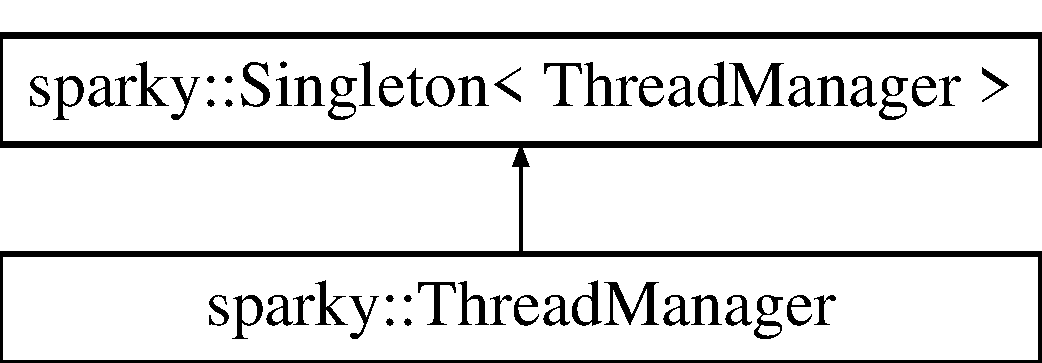
\includegraphics[height=2.000000cm]{classsparky_1_1_thread_manager}
\end{center}
\end{figure}
\subsection*{Public Member Functions}
\begin{DoxyCompactItemize}
\item 
\hyperlink{classsparky_1_1_thread_manager_a5442dd3baea9513c406b02e8a6b97b73}{$\sim$\+Thread\+Manager} (void)
\begin{DoxyCompactList}\small\item\em Destruction of the \hyperlink{classsparky_1_1_thread_manager}{Thread\+Manager} object. \end{DoxyCompactList}\item 
void \hyperlink{classsparky_1_1_thread_manager_ade9dc04071ece6e4aec12b5479dfbd53}{add\+Task} (const std\+::function$<$ void()$>$ \&function)
\begin{DoxyCompactList}\small\item\em Adds a task to the thread pool for execution. \end{DoxyCompactList}\end{DoxyCompactItemize}
\subsection*{Friends}
\begin{DoxyCompactItemize}
\item 
class {\bfseries Singleton$<$ Thread\+Manager $>$}\hypertarget{classsparky_1_1_thread_manager_a3c218ec0248bcc9ff4b63b9d988126d3}{}\label{classsparky_1_1_thread_manager_a3c218ec0248bcc9ff4b63b9d988126d3}

\end{DoxyCompactItemize}
\subsection*{Additional Inherited Members}


\subsection{Detailed Description}
\hyperlink{classsparky_1_1_thread_manager}{sparky\+::\+Thread\+Manager} is a singleton class which allows for global access to the applications thread pool. This global access allows for any function or method within the application to be multi-\/threaded and executed on a seperate thread.

\hyperlink{classsparky_1_1_thread_manager}{sparky\+::\+Thread\+Manager} is a global wrapper class for the thread pool. Below is a code example of using the Thread Manager.

Usage example\+: 
\begin{DoxyCode}
\textcolor{comment}{// Create a void function which just prints a statement.}
\textcolor{keywordtype}{void} printSentence(\textcolor{keywordtype}{void})
\{
    std::cout << \textcolor{stringliteral}{"Multi-threaded function!"} << std::endl;
\}

Adds the \textcolor{keyword}{function} to the thread manager.
sparky::ThreadManager::getInstance().addTask(printSentence);
\end{DoxyCode}
 

\subsection{Constructor \& Destructor Documentation}
\index{sparky\+::\+Thread\+Manager@{sparky\+::\+Thread\+Manager}!````~Thread\+Manager@{$\sim$\+Thread\+Manager}}
\index{````~Thread\+Manager@{$\sim$\+Thread\+Manager}!sparky\+::\+Thread\+Manager@{sparky\+::\+Thread\+Manager}}
\subsubsection[{\texorpdfstring{$\sim$\+Thread\+Manager(void)}{~ThreadManager(void)}}]{\setlength{\rightskip}{0pt plus 5cm}sparky\+::\+Thread\+Manager\+::$\sim$\+Thread\+Manager (
\begin{DoxyParamCaption}
\item[{void}]{}
\end{DoxyParamCaption}
)}\hypertarget{classsparky_1_1_thread_manager_a5442dd3baea9513c406b02e8a6b97b73}{}\label{classsparky_1_1_thread_manager_a5442dd3baea9513c406b02e8a6b97b73}


Destruction of the \hyperlink{classsparky_1_1_thread_manager}{Thread\+Manager} object. 

The destructor will join all of the currently active threads back to the main thread before de-\/allocation. 

\subsection{Member Function Documentation}
\index{sparky\+::\+Thread\+Manager@{sparky\+::\+Thread\+Manager}!add\+Task@{add\+Task}}
\index{add\+Task@{add\+Task}!sparky\+::\+Thread\+Manager@{sparky\+::\+Thread\+Manager}}
\subsubsection[{\texorpdfstring{add\+Task(const std\+::function$<$ void()$>$ \&function)}{addTask(const std::function< void()> &function)}}]{\setlength{\rightskip}{0pt plus 5cm}void sparky\+::\+Thread\+Manager\+::add\+Task (
\begin{DoxyParamCaption}
\item[{const std\+::function$<$ void()$>$ \&}]{function}
\end{DoxyParamCaption}
)}\hypertarget{classsparky_1_1_thread_manager_ade9dc04071ece6e4aec12b5479dfbd53}{}\label{classsparky_1_1_thread_manager_ade9dc04071ece6e4aec12b5479dfbd53}


Adds a task to the thread pool for execution. 

A task can be any function or method pointer in which void is specified as its return type. The function pointer allows for completely modular behaviour and tasks to be added to the task queue.


\begin{DoxyParams}{Parameters}
{\em function} & The function to execute on the threads. \\
\hline
\end{DoxyParams}


The documentation for this class was generated from the following file\+:\begin{DoxyCompactItemize}
\item 
C\+:/\+Users/\+Ben/\+Documents/repos/sparky/include/sparky/utils/threadmanager.\+hpp\end{DoxyCompactItemize}

\hypertarget{classsparky_1_1_thread_pool}{}\section{sparky\+:\+:Thread\+Pool Class Reference}
\label{classsparky_1_1_thread_pool}\index{sparky\+::\+Thread\+Pool@{sparky\+::\+Thread\+Pool}}


{\ttfamily \#include $<$threadpool.\+hpp$>$}

\subsection*{Public Member Functions}
\begin{DoxyCompactItemize}
\item 
\hyperlink{classsparky_1_1_thread_pool_ac153de2ca1a6b692c48e000c7891e439}{Thread\+Pool} (const unsigned int threads=std\+::thread\+::hardware\+\_\+concurrency())
\begin{DoxyCompactList}\small\item\em Constructs the Thread Pool with a set amount of threads. \end{DoxyCompactList}\item 
\hyperlink{classsparky_1_1_thread_pool_ae54a60ab84b11b3bb6dcccea9ba4d841}{$\sim$\+Thread\+Pool} (void)
\begin{DoxyCompactList}\small\item\em Destruction of the Thread Pool object. \end{DoxyCompactList}\item 
void \hyperlink{classsparky_1_1_thread_pool_a3faeacdbbab736f1461c7ea53739e34f}{add\+Task} (const std\+::function$<$ void()$>$ \&function)
\begin{DoxyCompactList}\small\item\em Adds a task that an inactive thread will execute. \end{DoxyCompactList}\item 
void \hyperlink{classsparky_1_1_thread_pool_a24ce7704a54be1f5b956d61bc6c0fc7f}{join} (void)
\begin{DoxyCompactList}\small\item\em Joins each thread back to the main thread. \end{DoxyCompactList}\end{DoxyCompactItemize}


\subsection{Detailed Description}
The Thread Pool is a convenience class for easily setting up multi-\/threaded applications and useability without having to over-\/complicate code bases and scatter locks. The thread pool will continuously run in the background of the application and process any tasks assigned to it.

This is useful for assigning tasks which may slow down certain elements of the engine, such as the chunk generation for the \hyperlink{classsparky_1_1_voxel}{Voxel} \hyperlink{classsparky_1_1_world}{World}. Below is an example of using the Pool without the Thread Manager.

Usage example\+: 
\begin{DoxyCode}
\textcolor{comment}{// Create a pool with the maximum amount of threads.}
\hyperlink{classsparky_1_1_thread_pool}{sparky::ThreadPool} pool;

\textcolor{comment}{// Add a task using a lambda function.}
\textcolor{keywordtype}{int} number = 5;
pool.\hyperlink{classsparky_1_1_thread_pool_a3faeacdbbab736f1461c7ea53739e34f}{addTask}([&number](\textcolor{keywordtype}{int} num) \{ number = num; \});

\textcolor{comment}{// Join the pool to the main thread.}
pool.\hyperlink{classsparky_1_1_thread_pool_a24ce7704a54be1f5b956d61bc6c0fc7f}{join}();
\end{DoxyCode}
 

\subsection{Constructor \& Destructor Documentation}
\index{sparky\+::\+Thread\+Pool@{sparky\+::\+Thread\+Pool}!Thread\+Pool@{Thread\+Pool}}
\index{Thread\+Pool@{Thread\+Pool}!sparky\+::\+Thread\+Pool@{sparky\+::\+Thread\+Pool}}
\subsubsection[{\texorpdfstring{Thread\+Pool(const unsigned int threads=std\+::thread\+::hardware\+\_\+concurrency())}{ThreadPool(const unsigned int threads=std::thread::hardware_concurrency())}}]{\setlength{\rightskip}{0pt plus 5cm}sparky\+::\+Thread\+Pool\+::\+Thread\+Pool (
\begin{DoxyParamCaption}
\item[{const unsigned int}]{threads = {\ttfamily std\+:\+:thread\+:\+:hardware\+\_\+concurrency()}}
\end{DoxyParamCaption}
)\hspace{0.3cm}{\ttfamily [explicit]}}\hypertarget{classsparky_1_1_thread_pool_ac153de2ca1a6b692c48e000c7891e439}{}\label{classsparky_1_1_thread_pool_ac153de2ca1a6b692c48e000c7891e439}


Constructs the Thread Pool with a set amount of threads. 

Default constructor of the Thread Pool object instance. The amount of threads that the pool will utilise is set by default to the maximum that the hardware can utilise. The user can specify if they wish to use less threads for the pool.


\begin{DoxyParams}{Parameters}
{\em threads} & The amount of threads that the pool will utilise. \\
\hline
\end{DoxyParams}
\index{sparky\+::\+Thread\+Pool@{sparky\+::\+Thread\+Pool}!````~Thread\+Pool@{$\sim$\+Thread\+Pool}}
\index{````~Thread\+Pool@{$\sim$\+Thread\+Pool}!sparky\+::\+Thread\+Pool@{sparky\+::\+Thread\+Pool}}
\subsubsection[{\texorpdfstring{$\sim$\+Thread\+Pool(void)}{~ThreadPool(void)}}]{\setlength{\rightskip}{0pt plus 5cm}sparky\+::\+Thread\+Pool\+::$\sim$\+Thread\+Pool (
\begin{DoxyParamCaption}
\item[{void}]{}
\end{DoxyParamCaption}
)}\hypertarget{classsparky_1_1_thread_pool_ae54a60ab84b11b3bb6dcccea9ba4d841}{}\label{classsparky_1_1_thread_pool_ae54a60ab84b11b3bb6dcccea9ba4d841}


Destruction of the Thread Pool object. 

Default destruction of the Thread Pool object instance. This will make sure that all of the threads have stopped before joining them back to the main thread. 

\subsection{Member Function Documentation}
\index{sparky\+::\+Thread\+Pool@{sparky\+::\+Thread\+Pool}!add\+Task@{add\+Task}}
\index{add\+Task@{add\+Task}!sparky\+::\+Thread\+Pool@{sparky\+::\+Thread\+Pool}}
\subsubsection[{\texorpdfstring{add\+Task(const std\+::function$<$ void()$>$ \&function)}{addTask(const std::function< void()> &function)}}]{\setlength{\rightskip}{0pt plus 5cm}void sparky\+::\+Thread\+Pool\+::add\+Task (
\begin{DoxyParamCaption}
\item[{const std\+::function$<$ void()$>$ \&}]{function}
\end{DoxyParamCaption}
)}\hypertarget{classsparky_1_1_thread_pool_a3faeacdbbab736f1461c7ea53739e34f}{}\label{classsparky_1_1_thread_pool_a3faeacdbbab736f1461c7ea53739e34f}


Adds a task that an inactive thread will execute. 

Adds a task to the queue of tasks that are to be executed by the threads within the pool. If no threads are currently available, it is added to a queue and executed as soon as possible.


\begin{DoxyParams}{Parameters}
{\em function} & The function that the threads will execute.\\
\hline
\end{DoxyParams}

\begin{DoxyRetVals}{Return values}
{\em future} & The future result of the added task. \\
\hline
\end{DoxyRetVals}
\index{sparky\+::\+Thread\+Pool@{sparky\+::\+Thread\+Pool}!join@{join}}
\index{join@{join}!sparky\+::\+Thread\+Pool@{sparky\+::\+Thread\+Pool}}
\subsubsection[{\texorpdfstring{join(void)}{join(void)}}]{\setlength{\rightskip}{0pt plus 5cm}void sparky\+::\+Thread\+Pool\+::join (
\begin{DoxyParamCaption}
\item[{void}]{}
\end{DoxyParamCaption}
)}\hypertarget{classsparky_1_1_thread_pool_a24ce7704a54be1f5b956d61bc6c0fc7f}{}\label{classsparky_1_1_thread_pool_a24ce7704a54be1f5b956d61bc6c0fc7f}


Joins each thread back to the main thread. 

This method is automatically called upon destruction of the Thread Pool. It joins all of the current threads within the pool and sets it stop multi-\/threading. 

The documentation for this class was generated from the following file\+:\begin{DoxyCompactItemize}
\item 
C\+:/\+Users/\+Ben/\+Documents/repos/sparky/include/sparky/utils/threadpool.\+hpp\end{DoxyCompactItemize}

\hypertarget{classsparky_1_1_time}{}\section{sparky\+:\+:Time Class Reference}
\label{classsparky_1_1_time}\index{sparky\+::\+Time@{sparky\+::\+Time}}


{\ttfamily \#include $<$time.\+hpp$>$}

\subsection*{Static Public Member Functions}
\begin{DoxyCompactItemize}
\item 
static float \hyperlink{classsparky_1_1_time_af216f91f65a7631ee3e1974a244f697b}{get\+Delta\+Time} (void)
\begin{DoxyCompactList}\small\item\em Retrieves the delta-\/time of the current frame. \end{DoxyCompactList}\item 
static void \hyperlink{classsparky_1_1_time_a9b56a371f5e1dda4fd9ee32c71d5855a}{start} (void)\hypertarget{classsparky_1_1_time_a9b56a371f5e1dda4fd9ee32c71d5855a}{}\label{classsparky_1_1_time_a9b56a371f5e1dda4fd9ee32c71d5855a}

\begin{DoxyCompactList}\small\item\em Starts the timer to calculate the beginning time of the current frame. \end{DoxyCompactList}\item 
static void \hyperlink{classsparky_1_1_time_acc429e19f42da5dee935a1d54d40ef8f}{stop} (void)\hypertarget{classsparky_1_1_time_acc429e19f42da5dee935a1d54d40ef8f}{}\label{classsparky_1_1_time_acc429e19f42da5dee935a1d54d40ef8f}

\begin{DoxyCompactList}\small\item\em Stops the timer and calculates the time that it took to render and update this frame, this value is stored in delta-\/time for use by other objects and instances. \end{DoxyCompactList}\end{DoxyCompactItemize}


\subsection{Detailed Description}
\hyperlink{classsparky_1_1_time}{sparky\+::\+Time} is responsible for tracking the delta-\/time of each frame. At the beginning of each frame, the timer is start and at the end of the frame, the timer is stopped and delta-\/time is calculated accordingly. Below is a code example.

Usage Example\+: 
\begin{DoxyCode}
\textcolor{comment}{// Start the timer.}
\hyperlink{classsparky_1_1_time_a9b56a371f5e1dda4fd9ee32c71d5855a}{Time::start}();

\textcolor{comment}{// Create a Transform object.}
\hyperlink{classsparky_1_1_transform}{sparky::Transform} transform;

\textcolor{comment}{// Apply a rotation to the transform by utilising delta-time for smooth rotation.}
\hyperlink{classsparky_1_1_quaternion}{sparky::Quaternionf} rotation = \hyperlink{classsparky_1_1_quaternion_a66ae7960536a332a5d2e133bb14bc5c5}{sparky::Quaternionf::angleAxis}
      (\hyperlink{classsparky_1_1_vector3_af54c2e1458f00c76b06c61641c856c95}{sparky::Vector3f::up}(), 5.0f * \hyperlink{classsparky_1_1_time_af216f91f65a7631ee3e1974a244f697b}{sparky::Time::getDeltaTime}());

\textcolor{comment}{// Apply the rotation to the transform object.}
transform.\hyperlink{classsparky_1_1_transform_af3b667562451c1cd254bb7708d15a2ce}{rotate}(rotation);

\textcolor{comment}{// Stop the timer.}
\hyperlink{classsparky_1_1_time_acc429e19f42da5dee935a1d54d40ef8f}{Time::stop}();
\end{DoxyCode}
 

\subsection{Member Function Documentation}
\index{sparky\+::\+Time@{sparky\+::\+Time}!get\+Delta\+Time@{get\+Delta\+Time}}
\index{get\+Delta\+Time@{get\+Delta\+Time}!sparky\+::\+Time@{sparky\+::\+Time}}
\subsubsection[{\texorpdfstring{get\+Delta\+Time(void)}{getDeltaTime(void)}}]{\setlength{\rightskip}{0pt plus 5cm}static float sparky\+::\+Time\+::get\+Delta\+Time (
\begin{DoxyParamCaption}
\item[{void}]{}
\end{DoxyParamCaption}
)\hspace{0.3cm}{\ttfamily [static]}}\hypertarget{classsparky_1_1_time_af216f91f65a7631ee3e1974a244f697b}{}\label{classsparky_1_1_time_af216f91f65a7631ee3e1974a244f697b}


Retrieves the delta-\/time of the current frame. 

The delta-\/time is calculated at the end of the current frame. It is the time that the frame took to render, update and process the input of the current frame.


\begin{DoxyRetVals}{Return values}
{\em float} & The current delta-\/time of the frame. \\
\hline
\end{DoxyRetVals}


The documentation for this class was generated from the following file\+:\begin{DoxyCompactItemize}
\item 
C\+:/\+Users/\+Ben/\+Documents/repos/sparky/include/sparky/core/time.\+hpp\end{DoxyCompactItemize}

\hypertarget{classsparky_1_1_transform}{}\section{sparky\+:\+:Transform Class Reference}
\label{classsparky_1_1_transform}\index{sparky\+::\+Transform@{sparky\+::\+Transform}}


{\ttfamily \#include $<$transform.\+hpp$>$}

\subsection*{Public Member Functions}
\begin{DoxyCompactItemize}
\item 
\hyperlink{classsparky_1_1_transform_abf5ec0c413c17786ce73f2b2071dbfc6}{Transform} (void)
\begin{DoxyCompactList}\small\item\em Default construction of the \hyperlink{classsparky_1_1_transform}{Transform} object. \end{DoxyCompactList}\item 
\hyperlink{classsparky_1_1_transform_ab769f038ba7536105ff683fffd58054d}{Transform} (const \hyperlink{classsparky_1_1_vector3}{Vector3f} \&position, const \hyperlink{classsparky_1_1_quaternion}{Quaternionf} \&rotation)
\begin{DoxyCompactList}\small\item\em Construction of the \hyperlink{classsparky_1_1_transform}{Transform} object with a set position and rotation. \end{DoxyCompactList}\item 
\hyperlink{classsparky_1_1_transform_ae221098b15225b919719b1ebb7f6b393}{Transform} (const \hyperlink{classsparky_1_1_vector3}{Vector3f} \&position, const \hyperlink{classsparky_1_1_vector3}{Vector3f} \&scale, const \hyperlink{classsparky_1_1_quaternion}{Quaternionf} \&rotation)
\begin{DoxyCompactList}\small\item\em Construction of the \hyperlink{classsparky_1_1_transform}{Transform} object with a set position, rotation and scale. \end{DoxyCompactList}\item 
\hyperlink{classsparky_1_1_transform_a5c9b5691d54c9572e67d560a82a0d483}{$\sim$\+Transform} (void)=default\hypertarget{classsparky_1_1_transform_a5c9b5691d54c9572e67d560a82a0d483}{}\label{classsparky_1_1_transform_a5c9b5691d54c9572e67d560a82a0d483}

\begin{DoxyCompactList}\small\item\em Default destruction of the \hyperlink{classsparky_1_1_transform}{Transform} object. \end{DoxyCompactList}\item 
\hyperlink{classsparky_1_1_vector3}{Vector3f} \hyperlink{classsparky_1_1_transform_add89b676d494ee5f5f5c45e82405127b}{get\+Position} (void) const 
\begin{DoxyCompactList}\small\item\em Retrieves the current translation of the \hyperlink{classsparky_1_1_transform}{Transform}. \end{DoxyCompactList}\item 
void \hyperlink{classsparky_1_1_transform_aff16fd5ad2157d604364a59835865d5c}{set\+Position} (const \hyperlink{classsparky_1_1_vector3}{Vector3f} \&position)
\begin{DoxyCompactList}\small\item\em Sets the position of the current \hyperlink{classsparky_1_1_transform}{Transform} to a new value. \end{DoxyCompactList}\item 
\hyperlink{classsparky_1_1_vector3}{Vector3f} \hyperlink{classsparky_1_1_transform_a0f32c05a0c33365df5cb58f03af43a59}{get\+Scale} (void) const 
\begin{DoxyCompactList}\small\item\em Retrieves the current scale of the \hyperlink{classsparky_1_1_transform}{Transform} object. \end{DoxyCompactList}\item 
void \hyperlink{classsparky_1_1_transform_af150a728b784dbcb73aefd653393083f}{set\+Scale} (const \hyperlink{classsparky_1_1_vector3}{Vector3f} \&scale)
\begin{DoxyCompactList}\small\item\em Sets the new scale of the \hyperlink{classsparky_1_1_transform}{Transform} object. \end{DoxyCompactList}\item 
\hyperlink{classsparky_1_1_quaternion}{Quaternionf} \hyperlink{classsparky_1_1_transform_a9f5febdbccb5bc718e1cfb2ff57e49f2}{get\+Rotation} (void) const 
\begin{DoxyCompactList}\small\item\em Retrieves the rotation of the current \hyperlink{classsparky_1_1_transform}{Transform} object. \end{DoxyCompactList}\item 
void \hyperlink{classsparky_1_1_transform_a870405b2aa4bd13ffa48a8e072f7bf3b}{set\+Rotation} (const \hyperlink{classsparky_1_1_quaternion}{Quaternionf} \&rotation)
\begin{DoxyCompactList}\small\item\em Sets a new rotation of the \hyperlink{classsparky_1_1_transform}{Transform} object. \end{DoxyCompactList}\item 
\hyperlink{classsparky_1_1_matrix4}{Matrix4f} \hyperlink{classsparky_1_1_transform_aa5c5aa2ded3b97e4f55a927e7b8f9bbf}{get\+Transformation} (void) const 
\begin{DoxyCompactList}\small\item\em Retrieves the transformation of the \hyperlink{classsparky_1_1_transform}{Transform} object. \end{DoxyCompactList}\item 
void \hyperlink{classsparky_1_1_transform_a2abf650641e50055dffaf6c11e4e5b79}{translate} (const \hyperlink{classsparky_1_1_vector3}{Vector3f} \&translation)
\begin{DoxyCompactList}\small\item\em Translates the position of the \hyperlink{classsparky_1_1_transform}{Transform} by the given amount. \end{DoxyCompactList}\item 
void \hyperlink{classsparky_1_1_transform_af3b667562451c1cd254bb7708d15a2ce}{rotate} (const \hyperlink{classsparky_1_1_quaternion}{Quaternionf} \&rotation)
\begin{DoxyCompactList}\small\item\em Rotates the current rotation of the \hyperlink{classsparky_1_1_transform}{Transform} by the specified amount. \end{DoxyCompactList}\item 
\hyperlink{classsparky_1_1_vector3}{Vector3f} \hyperlink{classsparky_1_1_transform_a50d2ed69775d32d034cf604cd48400a5}{right} (void) const 
\begin{DoxyCompactList}\small\item\em Retrieves the local right of the \hyperlink{classsparky_1_1_transform}{Transform} object. \end{DoxyCompactList}\item 
\hyperlink{classsparky_1_1_vector3}{Vector3f} \hyperlink{classsparky_1_1_transform_aae0c78bdcabf3980bd20c1b45b58ca57}{up} (void) const 
\begin{DoxyCompactList}\small\item\em Retrieves the local up of the \hyperlink{classsparky_1_1_transform}{Transform} object. \end{DoxyCompactList}\item 
\hyperlink{classsparky_1_1_vector3}{Vector3f} \hyperlink{classsparky_1_1_transform_ad8cc87e8a055e05c54ea0ead03376b21}{forward} (void) const 
\begin{DoxyCompactList}\small\item\em Retrieves the local forward of the \hyperlink{classsparky_1_1_transform}{Transform} object. \end{DoxyCompactList}\end{DoxyCompactItemize}


\subsection{Detailed Description}
\hyperlink{classsparky_1_1_transform}{sparky\+::\+Transform} is the culmination class for all of the mathematic functionality within the Sparky Engine. It is utilised with any object that needs a position, rotation and scale within 3D space.

The \hyperlink{classsparky_1_1_transform}{Transform} class is commonly used with the \hyperlink{classsparky_1_1_camera}{Camera} and \hyperlink{classsparky_1_1_chunk}{Chunk} classes. Below is a code example of using the \hyperlink{classsparky_1_1_transform}{Transform} class.

Usage example\+: 
\begin{DoxyCode}
\textcolor{comment}{// Create the position, rotation and scale of the object.}
\hyperlink{classsparky_1_1_vector3}{sparky::Vector3f} position(0.0f, 0.0f, 5.0f);
\hyperlink{classsparky_1_1_vector3}{sparky::Vector3f} scale(2.0f, 2.0f, 2.0f);
\hyperlink{classsparky_1_1_quaternion}{sparky::Quaternionf} rotation(0.0f, 0.0f, 0.0f, 1.0f);

\textcolor{comment}{// Create the Transform object with this information.}
\hyperlink{classsparky_1_1_transform}{sparky::Transform} transform(position, scale, rotation);

\textcolor{comment}{// Create rotation to rotate the transform by.}
\hyperlink{classsparky_1_1_quaternion}{sparky::Quaternionf} axis = \hyperlink{classsparky_1_1_quaternion_a66ae7960536a332a5d2e133bb14bc5c5}{sparky::Quaternionf::angleAxis}(
      \hyperlink{classsparky_1_1_vector3}{sparky::Vector3f}(0.0f, 1.0f, 0.0f), 5.0f * sparky::Time::getDeltaTime());

\textcolor{comment}{// Apply the rotation.}
transform.\hyperlink{classsparky_1_1_transform_af3b667562451c1cd254bb7708d15a2ce}{rotate}(axis);
\end{DoxyCode}
 

\subsection{Constructor \& Destructor Documentation}
\index{sparky\+::\+Transform@{sparky\+::\+Transform}!Transform@{Transform}}
\index{Transform@{Transform}!sparky\+::\+Transform@{sparky\+::\+Transform}}
\subsubsection[{\texorpdfstring{Transform(void)}{Transform(void)}}]{\setlength{\rightskip}{0pt plus 5cm}sparky\+::\+Transform\+::\+Transform (
\begin{DoxyParamCaption}
\item[{void}]{}
\end{DoxyParamCaption}
)\hspace{0.3cm}{\ttfamily [explicit]}}\hypertarget{classsparky_1_1_transform_abf5ec0c413c17786ce73f2b2071dbfc6}{}\label{classsparky_1_1_transform_abf5ec0c413c17786ce73f2b2071dbfc6}


Default construction of the \hyperlink{classsparky_1_1_transform}{Transform} object. 

The default construction of the \hyperlink{classsparky_1_1_transform}{Transform} will set the position, rotation and scale to default values \mbox{[} 0, 0, 0 \mbox{]}, \mbox{[} 1, 1, 1\mbox{]}, \mbox{[} 0, 0, 0, 1 \mbox{]}. \index{sparky\+::\+Transform@{sparky\+::\+Transform}!Transform@{Transform}}
\index{Transform@{Transform}!sparky\+::\+Transform@{sparky\+::\+Transform}}
\subsubsection[{\texorpdfstring{Transform(const Vector3f \&position, const Quaternionf \&rotation)}{Transform(const Vector3f &position, const Quaternionf &rotation)}}]{\setlength{\rightskip}{0pt plus 5cm}sparky\+::\+Transform\+::\+Transform (
\begin{DoxyParamCaption}
\item[{const {\bf Vector3f} \&}]{position, }
\item[{const {\bf Quaternionf} \&}]{rotation}
\end{DoxyParamCaption}
)\hspace{0.3cm}{\ttfamily [explicit]}}\hypertarget{classsparky_1_1_transform_ab769f038ba7536105ff683fffd58054d}{}\label{classsparky_1_1_transform_ab769f038ba7536105ff683fffd58054d}


Construction of the \hyperlink{classsparky_1_1_transform}{Transform} object with a set position and rotation. 

This constructor will create a \hyperlink{classsparky_1_1_transform}{Transform} object with an implicitly defined position and rotation. The scale is set to \mbox{[} 1, 1, 1 \mbox{]}.


\begin{DoxyParams}{Parameters}
{\em position} & The translation of the \hyperlink{classsparky_1_1_transform}{Transform} object. \\
\hline
{\em rotation} & The rotation of the \hyperlink{classsparky_1_1_transform}{Transform} object. \\
\hline
\end{DoxyParams}
\index{sparky\+::\+Transform@{sparky\+::\+Transform}!Transform@{Transform}}
\index{Transform@{Transform}!sparky\+::\+Transform@{sparky\+::\+Transform}}
\subsubsection[{\texorpdfstring{Transform(const Vector3f \&position, const Vector3f \&scale, const Quaternionf \&rotation)}{Transform(const Vector3f &position, const Vector3f &scale, const Quaternionf &rotation)}}]{\setlength{\rightskip}{0pt plus 5cm}sparky\+::\+Transform\+::\+Transform (
\begin{DoxyParamCaption}
\item[{const {\bf Vector3f} \&}]{position, }
\item[{const {\bf Vector3f} \&}]{scale, }
\item[{const {\bf Quaternionf} \&}]{rotation}
\end{DoxyParamCaption}
)\hspace{0.3cm}{\ttfamily [explicit]}}\hypertarget{classsparky_1_1_transform_ae221098b15225b919719b1ebb7f6b393}{}\label{classsparky_1_1_transform_ae221098b15225b919719b1ebb7f6b393}


Construction of the \hyperlink{classsparky_1_1_transform}{Transform} object with a set position, rotation and scale. 

This constructor will create a \hyperlink{classsparky_1_1_transform}{Transform} object with an implicitly defined position, scale and rotation.


\begin{DoxyParams}{Parameters}
{\em position} & The translation of the \hyperlink{classsparky_1_1_transform}{Transform} object. \\
\hline
{\em scale} & The scale of the \hyperlink{classsparky_1_1_transform}{Transform} object. \\
\hline
{\em rotation} & The rotation of the \hyperlink{classsparky_1_1_transform}{Transform} object. \\
\hline
\end{DoxyParams}


\subsection{Member Function Documentation}
\index{sparky\+::\+Transform@{sparky\+::\+Transform}!forward@{forward}}
\index{forward@{forward}!sparky\+::\+Transform@{sparky\+::\+Transform}}
\subsubsection[{\texorpdfstring{forward(void) const }{forward(void) const }}]{\setlength{\rightskip}{0pt plus 5cm}{\bf Vector3f} sparky\+::\+Transform\+::forward (
\begin{DoxyParamCaption}
\item[{void}]{}
\end{DoxyParamCaption}
) const}\hypertarget{classsparky_1_1_transform_ad8cc87e8a055e05c54ea0ead03376b21}{}\label{classsparky_1_1_transform_ad8cc87e8a055e05c54ea0ead03376b21}


Retrieves the local forward of the \hyperlink{classsparky_1_1_transform}{Transform} object. 


\begin{DoxyRetVals}{Return values}
{\em Vector3f} & The current forward axis of the \hyperlink{classsparky_1_1_transform}{Transform}. \\
\hline
\end{DoxyRetVals}
\index{sparky\+::\+Transform@{sparky\+::\+Transform}!get\+Position@{get\+Position}}
\index{get\+Position@{get\+Position}!sparky\+::\+Transform@{sparky\+::\+Transform}}
\subsubsection[{\texorpdfstring{get\+Position(void) const }{getPosition(void) const }}]{\setlength{\rightskip}{0pt plus 5cm}{\bf Vector3f} sparky\+::\+Transform\+::get\+Position (
\begin{DoxyParamCaption}
\item[{void}]{}
\end{DoxyParamCaption}
) const}\hypertarget{classsparky_1_1_transform_add89b676d494ee5f5f5c45e82405127b}{}\label{classsparky_1_1_transform_add89b676d494ee5f5f5c45e82405127b}


Retrieves the current translation of the \hyperlink{classsparky_1_1_transform}{Transform}. 

The position refers to the objects position within the 3D environment.


\begin{DoxyRetVals}{Return values}
{\em Vector3f} & The current position. \\
\hline
\end{DoxyRetVals}
\index{sparky\+::\+Transform@{sparky\+::\+Transform}!get\+Rotation@{get\+Rotation}}
\index{get\+Rotation@{get\+Rotation}!sparky\+::\+Transform@{sparky\+::\+Transform}}
\subsubsection[{\texorpdfstring{get\+Rotation(void) const }{getRotation(void) const }}]{\setlength{\rightskip}{0pt plus 5cm}{\bf Quaternionf} sparky\+::\+Transform\+::get\+Rotation (
\begin{DoxyParamCaption}
\item[{void}]{}
\end{DoxyParamCaption}
) const}\hypertarget{classsparky_1_1_transform_a9f5febdbccb5bc718e1cfb2ff57e49f2}{}\label{classsparky_1_1_transform_a9f5febdbccb5bc718e1cfb2ff57e49f2}


Retrieves the rotation of the current \hyperlink{classsparky_1_1_transform}{Transform} object. 

The rotation refers to the current orientation of the object. As the application uses Quaternions, there is no gimbal lock.


\begin{DoxyRetVals}{Return values}
{\em Quaternionf} & The current rotation of the \hyperlink{classsparky_1_1_transform}{Transform} object. \\
\hline
\end{DoxyRetVals}
\index{sparky\+::\+Transform@{sparky\+::\+Transform}!get\+Scale@{get\+Scale}}
\index{get\+Scale@{get\+Scale}!sparky\+::\+Transform@{sparky\+::\+Transform}}
\subsubsection[{\texorpdfstring{get\+Scale(void) const }{getScale(void) const }}]{\setlength{\rightskip}{0pt plus 5cm}{\bf Vector3f} sparky\+::\+Transform\+::get\+Scale (
\begin{DoxyParamCaption}
\item[{void}]{}
\end{DoxyParamCaption}
) const}\hypertarget{classsparky_1_1_transform_a0f32c05a0c33365df5cb58f03af43a59}{}\label{classsparky_1_1_transform_a0f32c05a0c33365df5cb58f03af43a59}


Retrieves the current scale of the \hyperlink{classsparky_1_1_transform}{Transform} object. 

The scale refers to how large the current object within the scene is.


\begin{DoxyRetVals}{Return values}
{\em Vector3f} & The current scale of the \hyperlink{classsparky_1_1_transform}{Transform}. \\
\hline
\end{DoxyRetVals}
\index{sparky\+::\+Transform@{sparky\+::\+Transform}!get\+Transformation@{get\+Transformation}}
\index{get\+Transformation@{get\+Transformation}!sparky\+::\+Transform@{sparky\+::\+Transform}}
\subsubsection[{\texorpdfstring{get\+Transformation(void) const }{getTransformation(void) const }}]{\setlength{\rightskip}{0pt plus 5cm}{\bf Matrix4f} sparky\+::\+Transform\+::get\+Transformation (
\begin{DoxyParamCaption}
\item[{void}]{}
\end{DoxyParamCaption}
) const}\hypertarget{classsparky_1_1_transform_aa5c5aa2ded3b97e4f55a927e7b8f9bbf}{}\label{classsparky_1_1_transform_aa5c5aa2ded3b97e4f55a927e7b8f9bbf}


Retrieves the transformation of the \hyperlink{classsparky_1_1_transform}{Transform} object. 

The transformation refers to the transformation matrix of the current \hyperlink{classsparky_1_1_transform}{Transform} object. The transformation matrix is the combined matrix of the translation, rotation and scale.


\begin{DoxyRetVals}{Return values}
{\em Matrix4f} & The transformation matrix of the \hyperlink{classsparky_1_1_transform}{Transform} object. \\
\hline
\end{DoxyRetVals}
\index{sparky\+::\+Transform@{sparky\+::\+Transform}!right@{right}}
\index{right@{right}!sparky\+::\+Transform@{sparky\+::\+Transform}}
\subsubsection[{\texorpdfstring{right(void) const }{right(void) const }}]{\setlength{\rightskip}{0pt plus 5cm}{\bf Vector3f} sparky\+::\+Transform\+::right (
\begin{DoxyParamCaption}
\item[{void}]{}
\end{DoxyParamCaption}
) const}\hypertarget{classsparky_1_1_transform_a50d2ed69775d32d034cf604cd48400a5}{}\label{classsparky_1_1_transform_a50d2ed69775d32d034cf604cd48400a5}


Retrieves the local right of the \hyperlink{classsparky_1_1_transform}{Transform} object. 


\begin{DoxyRetVals}{Return values}
{\em Vector3f} & The current right axis of the \hyperlink{classsparky_1_1_transform}{Transform}. \\
\hline
\end{DoxyRetVals}
\index{sparky\+::\+Transform@{sparky\+::\+Transform}!rotate@{rotate}}
\index{rotate@{rotate}!sparky\+::\+Transform@{sparky\+::\+Transform}}
\subsubsection[{\texorpdfstring{rotate(const Quaternionf \&rotation)}{rotate(const Quaternionf &rotation)}}]{\setlength{\rightskip}{0pt plus 5cm}void sparky\+::\+Transform\+::rotate (
\begin{DoxyParamCaption}
\item[{const {\bf Quaternionf} \&}]{rotation}
\end{DoxyParamCaption}
)}\hypertarget{classsparky_1_1_transform_af3b667562451c1cd254bb7708d15a2ce}{}\label{classsparky_1_1_transform_af3b667562451c1cd254bb7708d15a2ce}


Rotates the current rotation of the \hyperlink{classsparky_1_1_transform}{Transform} by the specified amount. 

The rotation will rotate the current rotation by the specified amount, this method is short hand for r = r $\ast$ t.


\begin{DoxyParams}{Parameters}
{\em rotation} & The amount to rotate the current rotation by. \\
\hline
\end{DoxyParams}
\index{sparky\+::\+Transform@{sparky\+::\+Transform}!set\+Position@{set\+Position}}
\index{set\+Position@{set\+Position}!sparky\+::\+Transform@{sparky\+::\+Transform}}
\subsubsection[{\texorpdfstring{set\+Position(const Vector3f \&position)}{setPosition(const Vector3f &position)}}]{\setlength{\rightskip}{0pt plus 5cm}void sparky\+::\+Transform\+::set\+Position (
\begin{DoxyParamCaption}
\item[{const {\bf Vector3f} \&}]{position}
\end{DoxyParamCaption}
)}\hypertarget{classsparky_1_1_transform_aff16fd5ad2157d604364a59835865d5c}{}\label{classsparky_1_1_transform_aff16fd5ad2157d604364a59835865d5c}


Sets the position of the current \hyperlink{classsparky_1_1_transform}{Transform} to a new value. 

The position refers to the objects position within the 3D environment.


\begin{DoxyParams}{Parameters}
{\em position} & The new position of the \hyperlink{classsparky_1_1_transform}{Transform} object. \\
\hline
\end{DoxyParams}
\index{sparky\+::\+Transform@{sparky\+::\+Transform}!set\+Rotation@{set\+Rotation}}
\index{set\+Rotation@{set\+Rotation}!sparky\+::\+Transform@{sparky\+::\+Transform}}
\subsubsection[{\texorpdfstring{set\+Rotation(const Quaternionf \&rotation)}{setRotation(const Quaternionf &rotation)}}]{\setlength{\rightskip}{0pt plus 5cm}void sparky\+::\+Transform\+::set\+Rotation (
\begin{DoxyParamCaption}
\item[{const {\bf Quaternionf} \&}]{rotation}
\end{DoxyParamCaption}
)}\hypertarget{classsparky_1_1_transform_a870405b2aa4bd13ffa48a8e072f7bf3b}{}\label{classsparky_1_1_transform_a870405b2aa4bd13ffa48a8e072f7bf3b}


Sets a new rotation of the \hyperlink{classsparky_1_1_transform}{Transform} object. 

The rotation refers to the current orientation of the object. As the application uses Quaternions, there is no gimbal lock.


\begin{DoxyParams}{Parameters}
{\em rotation} & The new rotation of the \hyperlink{classsparky_1_1_transform}{Transform}. \\
\hline
\end{DoxyParams}
\index{sparky\+::\+Transform@{sparky\+::\+Transform}!set\+Scale@{set\+Scale}}
\index{set\+Scale@{set\+Scale}!sparky\+::\+Transform@{sparky\+::\+Transform}}
\subsubsection[{\texorpdfstring{set\+Scale(const Vector3f \&scale)}{setScale(const Vector3f &scale)}}]{\setlength{\rightskip}{0pt plus 5cm}void sparky\+::\+Transform\+::set\+Scale (
\begin{DoxyParamCaption}
\item[{const {\bf Vector3f} \&}]{scale}
\end{DoxyParamCaption}
)}\hypertarget{classsparky_1_1_transform_af150a728b784dbcb73aefd653393083f}{}\label{classsparky_1_1_transform_af150a728b784dbcb73aefd653393083f}


Sets the new scale of the \hyperlink{classsparky_1_1_transform}{Transform} object. 

The scale refers to how large the current object within the scene is.


\begin{DoxyParams}{Parameters}
{\em scale} & The new scale of the \hyperlink{classsparky_1_1_transform}{Transform} object. \\
\hline
\end{DoxyParams}
\index{sparky\+::\+Transform@{sparky\+::\+Transform}!translate@{translate}}
\index{translate@{translate}!sparky\+::\+Transform@{sparky\+::\+Transform}}
\subsubsection[{\texorpdfstring{translate(const Vector3f \&translation)}{translate(const Vector3f &translation)}}]{\setlength{\rightskip}{0pt plus 5cm}void sparky\+::\+Transform\+::translate (
\begin{DoxyParamCaption}
\item[{const {\bf Vector3f} \&}]{translation}
\end{DoxyParamCaption}
)}\hypertarget{classsparky_1_1_transform_a2abf650641e50055dffaf6c11e4e5b79}{}\label{classsparky_1_1_transform_a2abf650641e50055dffaf6c11e4e5b79}


Translates the position of the \hyperlink{classsparky_1_1_transform}{Transform} by the given amount. 

The translation will translate the current position by the specified amount, this method is just a convenience method for calculating p = p + t.


\begin{DoxyParams}{Parameters}
{\em translation} & The amount to move the current position by. \\
\hline
\end{DoxyParams}
\index{sparky\+::\+Transform@{sparky\+::\+Transform}!up@{up}}
\index{up@{up}!sparky\+::\+Transform@{sparky\+::\+Transform}}
\subsubsection[{\texorpdfstring{up(void) const }{up(void) const }}]{\setlength{\rightskip}{0pt plus 5cm}{\bf Vector3f} sparky\+::\+Transform\+::up (
\begin{DoxyParamCaption}
\item[{void}]{}
\end{DoxyParamCaption}
) const}\hypertarget{classsparky_1_1_transform_aae0c78bdcabf3980bd20c1b45b58ca57}{}\label{classsparky_1_1_transform_aae0c78bdcabf3980bd20c1b45b58ca57}


Retrieves the local up of the \hyperlink{classsparky_1_1_transform}{Transform} object. 


\begin{DoxyRetVals}{Return values}
{\em Vector3f} & The current up axis of the \hyperlink{classsparky_1_1_transform}{Transform}. \\
\hline
\end{DoxyRetVals}


The documentation for this class was generated from the following file\+:\begin{DoxyCompactItemize}
\item 
C\+:/\+Users/\+Ben/\+Documents/repos/sparky/include/sparky/math/transform.\+hpp\end{DoxyCompactItemize}

\hypertarget{classsparky_1_1_uniform}{}\section{sparky\+:\+:Uniform Class Reference}
\label{classsparky_1_1_uniform}\index{sparky\+::\+Uniform@{sparky\+::\+Uniform}}


{\ttfamily \#include $<$uniform.\+hpp$>$}

\subsection*{Public Member Functions}
\begin{DoxyCompactItemize}
\item 
\hyperlink{classsparky_1_1_uniform_affc278498dc526c133c2133106cfbf83}{Uniform} (\hyperlink{classsparky_1_1_program}{Program} $\ast$p\+Program)
\begin{DoxyCompactList}\small\item\em \hyperlink{classsparky_1_1_uniform}{Uniform} object constructor. \end{DoxyCompactList}\item 
\hyperlink{classsparky_1_1_uniform_a612d7e16c60770dba6a93f4fa2f79983}{$\sim$\+Uniform} (void)=default\hypertarget{classsparky_1_1_uniform_a612d7e16c60770dba6a93f4fa2f79983}{}\label{classsparky_1_1_uniform_a612d7e16c60770dba6a93f4fa2f79983}

\begin{DoxyCompactList}\small\item\em Default destructor for \hyperlink{classsparky_1_1_uniform}{Uniform} object. \end{DoxyCompactList}\item 
{\footnotesize template$<$typename T $>$ }\\void \hyperlink{classsparky_1_1_uniform_a7a81c72ed894749245b0f2b52fccd203}{set\+Parameter} (const \hyperlink{classsparky_1_1_string}{String} \&name, T \&\&value) const 
\begin{DoxyCompactList}\small\item\em Sends a value ( by name ) to the programs shaders. \end{DoxyCompactList}\end{DoxyCompactItemize}


\subsection{Detailed Description}
\hyperlink{classsparky_1_1_uniform}{sparky\+::\+Uniform} is convenience class for setting the values of uniform variables within a shader. \hyperlink{classsparky_1_1_uniform}{sparky\+::\+Uniform} provides overrides for all of the most of common G\+L\+SL types. Below is a code example\+:

Usage example\+: 
\begin{DoxyCode}
\textcolor{comment}{// Make a program and add shaders.}
\hyperlink{classsparky_1_1_program}{sparky::Program} program;

program.\hyperlink{classsparky_1_1_program_ac60e7883dc4076f78c3bcc1d5519f7e7}{attachShader}(\textcolor{keyword}{new} \hyperlink{classsparky_1_1_g_l_s_l_object}{sparky::GLSLObject}(\textcolor{stringliteral}{"shaders/basic\_vertex.glsl"},   
      sparky::eShaderType::VERTEX\_SHADER));
program.\hyperlink{classsparky_1_1_program_ac60e7883dc4076f78c3bcc1d5519f7e7}{attachShader}(\textcolor{keyword}{new} \hyperlink{classsparky_1_1_g_l_s_l_object}{sparky::GLSLObject}(\textcolor{stringliteral}{"shaders/basic\_fragment.glsl"}, 
      sparky::eShaderType::FRAGMENT\_SHADER));

\textcolor{comment}{// Link and compile the shaders.}
program.\hyperlink{classsparky_1_1_program_a7cbc014919fdcca3889edb283fbd4115}{link}();

\textcolor{comment}{// Sets a matrix within the shader to a identity matrix.}
\hyperlink{classsparky_1_1_matrix4}{sparky::Matrix4f} identity = \hyperlink{classsparky_1_1_matrix4_a0c11da6de697550bccdbf7de0976b08e}{sparky::Matrix4f::identity}();

\textcolor{comment}{// Send the matrix to the shaders.}
\hyperlink{classsparky_1_1_uniform}{sparky::Uniform} uniform(&program);

uniform.setParamater(\textcolor{stringliteral}{"matrix"}, identity);
\end{DoxyCode}
 

\subsection{Constructor \& Destructor Documentation}
\index{sparky\+::\+Uniform@{sparky\+::\+Uniform}!Uniform@{Uniform}}
\index{Uniform@{Uniform}!sparky\+::\+Uniform@{sparky\+::\+Uniform}}
\subsubsection[{\texorpdfstring{Uniform(\+Program $\ast$p\+Program)}{Uniform(Program *pProgram)}}]{\setlength{\rightskip}{0pt plus 5cm}sparky\+::\+Uniform\+::\+Uniform (
\begin{DoxyParamCaption}
\item[{{\bf Program} $\ast$}]{p\+Program}
\end{DoxyParamCaption}
)\hspace{0.3cm}{\ttfamily [explicit]}}\hypertarget{classsparky_1_1_uniform_affc278498dc526c133c2133106cfbf83}{}\label{classsparky_1_1_uniform_affc278498dc526c133c2133106cfbf83}


\hyperlink{classsparky_1_1_uniform}{Uniform} object constructor. 

\hyperlink{classsparky_1_1_uniform}{Uniform} needs access to the \hyperlink{classsparky_1_1_program}{Program} and its shader so it can successfully send uniforms to the shader for use.


\begin{DoxyParams}{Parameters}
{\em p\+Program} & The program containing the shaders. \\
\hline
\end{DoxyParams}


\subsection{Member Function Documentation}
\index{sparky\+::\+Uniform@{sparky\+::\+Uniform}!set\+Parameter@{set\+Parameter}}
\index{set\+Parameter@{set\+Parameter}!sparky\+::\+Uniform@{sparky\+::\+Uniform}}
\subsubsection[{\texorpdfstring{set\+Parameter(const String \&name, T \&\&value) const }{setParameter(const String &name, T &&value) const }}]{\setlength{\rightskip}{0pt plus 5cm}template$<$typename T $>$ void sparky\+::\+Uniform\+::set\+Parameter (
\begin{DoxyParamCaption}
\item[{const {\bf String} \&}]{name, }
\item[{T \&\&}]{value}
\end{DoxyParamCaption}
) const\hspace{0.3cm}{\ttfamily [inline]}}\hypertarget{classsparky_1_1_uniform_a7a81c72ed894749245b0f2b52fccd203}{}\label{classsparky_1_1_uniform_a7a81c72ed894749245b0f2b52fccd203}


Sends a value ( by name ) to the programs shaders. 


\begin{DoxyParams}{Parameters}
{\em name} & The name of the uniform in the shader. \\
\hline
{\em value} & The value to send to the shader. \\
\hline
\end{DoxyParams}


The documentation for this class was generated from the following file\+:\begin{DoxyCompactItemize}
\item 
C\+:/\+Users/\+Ben/\+Documents/repos/sparky/include/sparky/rendering/uniform.\+hpp\end{DoxyCompactItemize}

\hypertarget{classsparky_1_1_vector2}{}\section{sparky\+:\+:Vector2$<$ T $>$ Class Template Reference}
\label{classsparky_1_1_vector2}\index{sparky\+::\+Vector2$<$ T $>$@{sparky\+::\+Vector2$<$ T $>$}}
\subsection*{Public Member Functions}
\begin{DoxyCompactItemize}
\item 
\hyperlink{classsparky_1_1_vector2_aa6a3f1229ccd787a0622804cd3f2e64c}{Vector2} (void)\hypertarget{classsparky_1_1_vector2_aa6a3f1229ccd787a0622804cd3f2e64c}{}\label{classsparky_1_1_vector2_aa6a3f1229ccd787a0622804cd3f2e64c}

\begin{DoxyCompactList}\small\item\em Default contruction of \hyperlink{classsparky_1_1_vector2}{Vector2} object. \mbox{[} 0, 0 \mbox{]}. \end{DoxyCompactList}\item 
\hyperlink{classsparky_1_1_vector2_a89ef194a6a607f9f48dc9c54e2c498c0}{Vector2} (const T \hyperlink{classsparky_1_1_vector2_a30306429883f3c66f7f0170cab1b3cdf}{x}, const T \hyperlink{classsparky_1_1_vector2_ad56ad07afb25296661c4ded07a5a795c}{y})
\begin{DoxyCompactList}\small\item\em Constructs a \hyperlink{classsparky_1_1_vector2}{Vector2} object with defined x and y values. \end{DoxyCompactList}\item 
{\footnotesize template$<$typename U $>$ }\\\hyperlink{classsparky_1_1_vector2_a8de6450cda4e59e6e54bbca63a38cc00}{Vector2} (const \hyperlink{classsparky_1_1_vector2}{Vector2}$<$ U $>$ \&vector)
\begin{DoxyCompactList}\small\item\em Constructs a \hyperlink{classsparky_1_1_vector2}{Vector2} object from the members of a different \hyperlink{classsparky_1_1_vector2}{Vector2}. \end{DoxyCompactList}\item 
\hyperlink{classsparky_1_1_vector2_a55c70c9bffcbad505f3acf18b93b4e25}{$\sim$\+Vector2} (void)=default\hypertarget{classsparky_1_1_vector2_a55c70c9bffcbad505f3acf18b93b4e25}{}\label{classsparky_1_1_vector2_a55c70c9bffcbad505f3acf18b93b4e25}

\begin{DoxyCompactList}\small\item\em Default Vector destruction. \end{DoxyCompactList}\item 
\hyperlink{classsparky_1_1_vector2}{Vector2} \hyperlink{classsparky_1_1_vector2_a9bbccccae4177bf66b92361467499483}{operator+} (const \hyperlink{classsparky_1_1_vector2}{Vector2} \&vector) const 
\begin{DoxyCompactList}\small\item\em Addition operator between two Vectors. \end{DoxyCompactList}\item 
\hyperlink{classsparky_1_1_vector2}{Vector2} \hyperlink{classsparky_1_1_vector2_adeba5a6db0e22c6c5a7b2c8c4ad32997}{operator+} (const T value) const 
\begin{DoxyCompactList}\small\item\em Addition operator between a Vector and a value. \end{DoxyCompactList}\item 
\hyperlink{classsparky_1_1_vector2}{Vector2} \hyperlink{classsparky_1_1_vector2_adf06d5cdd7f79a3ba3add3ec99c54a8d}{operator-\/} (const \hyperlink{classsparky_1_1_vector2}{Vector2} \&vector) const 
\begin{DoxyCompactList}\small\item\em Subtraction operator between two Vectors. \end{DoxyCompactList}\item 
\hyperlink{classsparky_1_1_vector2}{Vector2} \hyperlink{classsparky_1_1_vector2_a7c9eb262606abaafe7c1aeff4d940e82}{operator-\/} (const T value) const 
\begin{DoxyCompactList}\small\item\em Subtraction operator between a Vector and a value. \end{DoxyCompactList}\item 
\hyperlink{classsparky_1_1_vector2}{Vector2} \hyperlink{classsparky_1_1_vector2_aeab66fc5fe4f5084064d0daf46916c1b}{operator$\ast$} (const \hyperlink{classsparky_1_1_vector2}{Vector2} \&vector) const 
\begin{DoxyCompactList}\small\item\em Multiplication operator between two Vectors. \end{DoxyCompactList}\item 
\hyperlink{classsparky_1_1_vector2}{Vector2} \hyperlink{classsparky_1_1_vector2_ab32ed07efc65a6a4bb8faae76e49870c}{operator$\ast$} (const T value) const 
\begin{DoxyCompactList}\small\item\em Multiplication operator between a Vector and a value. \end{DoxyCompactList}\item 
\hyperlink{classsparky_1_1_vector2}{Vector2} \hyperlink{classsparky_1_1_vector2_a10c66d9ba7d64bc64ac5243ce23c20db}{operator/} (const \hyperlink{classsparky_1_1_vector2}{Vector2} \&vector) const 
\begin{DoxyCompactList}\small\item\em Division operator between two Vectors. \end{DoxyCompactList}\item 
\hyperlink{classsparky_1_1_vector2}{Vector2} \hyperlink{classsparky_1_1_vector2_ab1a4d2950cb691643487dd86a41ab392}{operator/} (const T value) const 
\begin{DoxyCompactList}\small\item\em Division operator between a Vector and a value. \end{DoxyCompactList}\item 
const \hyperlink{classsparky_1_1_vector2}{Vector2} \& \hyperlink{classsparky_1_1_vector2_a3b7e4256f56c387e53c801c485ec15fd}{operator+=} (const \hyperlink{classsparky_1_1_vector2}{Vector2} \&vector)
\begin{DoxyCompactList}\small\item\em Addition operator between two Vectors. \end{DoxyCompactList}\item 
const \hyperlink{classsparky_1_1_vector2}{Vector2} \& \hyperlink{classsparky_1_1_vector2_ac614212b964b4d2d79442501b7e0c79e}{operator+=} (const T value)
\begin{DoxyCompactList}\small\item\em Addition operator between a Vector and value. \end{DoxyCompactList}\item 
const \hyperlink{classsparky_1_1_vector2}{Vector2} \& \hyperlink{classsparky_1_1_vector2_a89bef442fe29ac65a67e04ae3bba030a}{operator-\/=} (const \hyperlink{classsparky_1_1_vector2}{Vector2} \&vector)
\begin{DoxyCompactList}\small\item\em Subtraction operator between two Vectors. \end{DoxyCompactList}\item 
const \hyperlink{classsparky_1_1_vector2}{Vector2} \& \hyperlink{classsparky_1_1_vector2_ae5eb6cdc0c4e1c95a519e0b003432beb}{operator-\/=} (const T value)
\begin{DoxyCompactList}\small\item\em Subtraction operator between a Vector and value. \end{DoxyCompactList}\item 
const \hyperlink{classsparky_1_1_vector2}{Vector2} \& \hyperlink{classsparky_1_1_vector2_aa4e10696086e1fcefb03a9debc26da97}{operator$\ast$=} (const \hyperlink{classsparky_1_1_vector2}{Vector2} \&vector)
\begin{DoxyCompactList}\small\item\em Multiplication operator between two Vectors. \end{DoxyCompactList}\item 
const \hyperlink{classsparky_1_1_vector2}{Vector2} \& \hyperlink{classsparky_1_1_vector2_aefa9b779fc3f10462c4a9309934bb9d6}{operator$\ast$=} (const T value)
\begin{DoxyCompactList}\small\item\em Multiplication operator between a Vector and value. \end{DoxyCompactList}\item 
const \hyperlink{classsparky_1_1_vector2}{Vector2} \& \hyperlink{classsparky_1_1_vector2_a3529175fc7ec7ea46bb10e300f76f293}{operator/=} (const \hyperlink{classsparky_1_1_vector2}{Vector2} \&vector)
\begin{DoxyCompactList}\small\item\em Division operator between two Vectors. \end{DoxyCompactList}\item 
const \hyperlink{classsparky_1_1_vector2}{Vector2} \& \hyperlink{classsparky_1_1_vector2_a767b599519b6d4d5b23c94c65dc10806}{operator/=} (const T value)
\begin{DoxyCompactList}\small\item\em Division operator between a Vector and value. \end{DoxyCompactList}\item 
bool \hyperlink{classsparky_1_1_vector2_a96e356362b5d586662f9c015e1a5a929}{operator==} (const \hyperlink{classsparky_1_1_vector2}{Vector2} \&vector) const 
\begin{DoxyCompactList}\small\item\em Equality operation between two vectors. \end{DoxyCompactList}\item 
bool \hyperlink{classsparky_1_1_vector2_af18e1a53fd7f7bfd69ef0d2ebeab314f}{operator!=} (const \hyperlink{classsparky_1_1_vector2}{Vector2} \&vector) const 
\begin{DoxyCompactList}\small\item\em Non-\/\+Equality operation between two vectors. \end{DoxyCompactList}\item 
\hyperlink{classsparky_1_1_vector2}{Vector2} \hyperlink{classsparky_1_1_vector2_a6a40c2389b0f97186b41b0c559a6c800}{operator-\/} (void) const 
\begin{DoxyCompactList}\small\item\em Unary Operation on a Vector object. \end{DoxyCompactList}\item 
T \hyperlink{classsparky_1_1_vector2_a41ca66495f18b3a033fa679878ebd89e}{magnitude\+Sqr} (void) const 
\begin{DoxyCompactList}\small\item\em Calculates the squared length of the Vector object. \end{DoxyCompactList}\item 
T \hyperlink{classsparky_1_1_vector2_a04e90257c8bced3f650094807c82f6e8}{magnitude} (void) const 
\begin{DoxyCompactList}\small\item\em Calculates the length of the Vector object. \end{DoxyCompactList}\item 
\hyperlink{classsparky_1_1_vector2}{Vector2} \hyperlink{classsparky_1_1_vector2_a683c081fc98603639cb7129e5b97ec36}{normalised} (void)
\begin{DoxyCompactList}\small\item\em Calculates the unit length of the Vector object. \end{DoxyCompactList}\end{DoxyCompactItemize}
\subsection*{Static Public Member Functions}
\begin{DoxyCompactItemize}
\item 
static T \hyperlink{classsparky_1_1_vector2_aaf94222514e04f14673540c1b5619ba1}{dot} (const \hyperlink{classsparky_1_1_vector2}{Vector2} \&u, const \hyperlink{classsparky_1_1_vector2}{Vector2} \&v)
\begin{DoxyCompactList}\small\item\em Calculate the cosine angle between two Vector objects. \end{DoxyCompactList}\item 
static T \hyperlink{classsparky_1_1_vector2_ae9b8e7806712b2e7a21090f5804af7e8}{angle} (const \hyperlink{classsparky_1_1_vector2}{Vector2} \&from, const \hyperlink{classsparky_1_1_vector2}{Vector2} \&to)
\begin{DoxyCompactList}\small\item\em Gets the (degrees) angle between two Vector objects. \end{DoxyCompactList}\item 
static T \hyperlink{classsparky_1_1_vector2_a993818c0e8558a001cdf44a876149776}{distance\+Sqr} (const \hyperlink{classsparky_1_1_vector2}{Vector2} \&from, const \hyperlink{classsparky_1_1_vector2}{Vector2} \&to)
\begin{DoxyCompactList}\small\item\em Retrieves the squared euclidean distance between two different Vectors. \end{DoxyCompactList}\item 
static T \hyperlink{classsparky_1_1_vector2_a128195f83e6ae893c2299ba3cd852956}{distance} (const \hyperlink{classsparky_1_1_vector2}{Vector2} \&from, const \hyperlink{classsparky_1_1_vector2}{Vector2} \&to)
\begin{DoxyCompactList}\small\item\em Retrieves the euclidean distance between two different Vectors. \end{DoxyCompactList}\item 
static \hyperlink{classsparky_1_1_vector2}{Vector2} \hyperlink{classsparky_1_1_vector2_ad97f9078398cfa49dd75280d5d3f40a2}{minimum} (const \hyperlink{classsparky_1_1_vector2}{Vector2} \&u, const \hyperlink{classsparky_1_1_vector2}{Vector2} \&v)
\begin{DoxyCompactList}\small\item\em Gets the minimum values of two Vector objects. \end{DoxyCompactList}\item 
static \hyperlink{classsparky_1_1_vector2}{Vector2} \hyperlink{classsparky_1_1_vector2_a840bc220a702dc7c0649433682439282}{maximum} (const \hyperlink{classsparky_1_1_vector2}{Vector2} \&u, const \hyperlink{classsparky_1_1_vector2}{Vector2} \&v)
\begin{DoxyCompactList}\small\item\em Gets the maximum values of two Vector objects. \end{DoxyCompactList}\item 
static \hyperlink{classsparky_1_1_vector2}{Vector2} \hyperlink{classsparky_1_1_vector2_a11fff3da3ab0999fbca089993a776342}{move\+Towards} (const \hyperlink{classsparky_1_1_vector2}{Vector2} \&current, const \hyperlink{classsparky_1_1_vector2}{Vector2} \&target, const T speed)
\begin{DoxyCompactList}\small\item\em Moves a Vector towards the target. \end{DoxyCompactList}\item 
static \hyperlink{classsparky_1_1_vector2}{Vector2} \hyperlink{classsparky_1_1_vector2_aaa23250d4a657cb48f79adbfe14780be}{lerp} (const \hyperlink{classsparky_1_1_vector2}{Vector2} \&current, const \hyperlink{classsparky_1_1_vector2}{Vector2} \&target, const T speed)
\begin{DoxyCompactList}\small\item\em Vector linear interpolation. \end{DoxyCompactList}\item 
static \hyperlink{classsparky_1_1_vector2}{Vector2} \hyperlink{classsparky_1_1_vector2_a9481a8847391cca7213def01a65be4b8}{zero} (void)
\begin{DoxyCompactList}\small\item\em Convenience method for initialising a Vector to \mbox{[} 0, 0 \mbox{]}. \end{DoxyCompactList}\item 
static \hyperlink{classsparky_1_1_vector2}{Vector2} \hyperlink{classsparky_1_1_vector2_acbe0ab8fb2dcb29fdd176a328334b5fc}{one} (void)
\begin{DoxyCompactList}\small\item\em Convenience method for initialising a Vector to \mbox{[} 1, 1 \mbox{]}. \end{DoxyCompactList}\item 
static \hyperlink{classsparky_1_1_vector2}{Vector2} \hyperlink{classsparky_1_1_vector2_a27f5f4198db28574f00e9f63c9a27daf}{right} (void)
\begin{DoxyCompactList}\small\item\em Convenience method for initialising a Vector to \mbox{[} 1, 0 \mbox{]}. \end{DoxyCompactList}\item 
static \hyperlink{classsparky_1_1_vector2}{Vector2} \hyperlink{classsparky_1_1_vector2_ac5daaf099b7019f0925d9c812bbbcf4d}{up} (void)
\begin{DoxyCompactList}\small\item\em Convenience method for initialising a Vector to \mbox{[} 0, 1 \mbox{]}. \end{DoxyCompactList}\end{DoxyCompactItemize}
\subsection*{Public Attributes}
\begin{DoxyCompactItemize}
\item 
T \hyperlink{classsparky_1_1_vector2_a30306429883f3c66f7f0170cab1b3cdf}{x}\hypertarget{classsparky_1_1_vector2_a30306429883f3c66f7f0170cab1b3cdf}{}\label{classsparky_1_1_vector2_a30306429883f3c66f7f0170cab1b3cdf}

\begin{DoxyCompactList}\small\item\em The x (right) value. \end{DoxyCompactList}\item 
T \hyperlink{classsparky_1_1_vector2_ad56ad07afb25296661c4ded07a5a795c}{y}\hypertarget{classsparky_1_1_vector2_ad56ad07afb25296661c4ded07a5a795c}{}\label{classsparky_1_1_vector2_ad56ad07afb25296661c4ded07a5a795c}

\begin{DoxyCompactList}\small\item\em The y (up) value. \end{DoxyCompactList}\end{DoxyCompactItemize}
\subsection*{Friends}
\begin{DoxyCompactItemize}
\item 
std\+::ostream \& \hyperlink{classsparky_1_1_vector2_a9fc2efab2b5d63c84f76fa8f036bec0c}{operator$<$$<$} (std\+::ostream \&os, const \hyperlink{classsparky_1_1_vector2}{Vector2} \&vector)
\begin{DoxyCompactList}\small\item\em Overload the output stream operator to print a \hyperlink{classsparky_1_1_vector2}{Vector2} to the console window. \end{DoxyCompactList}\end{DoxyCompactItemize}


\subsection{Constructor \& Destructor Documentation}
\index{sparky\+::\+Vector2@{sparky\+::\+Vector2}!Vector2@{Vector2}}
\index{Vector2@{Vector2}!sparky\+::\+Vector2@{sparky\+::\+Vector2}}
\subsubsection[{\texorpdfstring{Vector2(const T x, const T y)}{Vector2(const T x, const T y)}}]{\setlength{\rightskip}{0pt plus 5cm}template$<$typename T$>$ {\bf sparky\+::\+Vector2}$<$ T $>$\+::{\bf Vector2} (
\begin{DoxyParamCaption}
\item[{const T}]{x, }
\item[{const T}]{y}
\end{DoxyParamCaption}
)\hspace{0.3cm}{\ttfamily [explicit]}}\hypertarget{classsparky_1_1_vector2_a89ef194a6a607f9f48dc9c54e2c498c0}{}\label{classsparky_1_1_vector2_a89ef194a6a607f9f48dc9c54e2c498c0}


Constructs a \hyperlink{classsparky_1_1_vector2}{Vector2} object with defined x and y values. 


\begin{DoxyParams}{Parameters}
{\em x} & The x value of the Vector object. \\
\hline
{\em y} & The y value of the Vector object. \\
\hline
\end{DoxyParams}
\index{sparky\+::\+Vector2@{sparky\+::\+Vector2}!Vector2@{Vector2}}
\index{Vector2@{Vector2}!sparky\+::\+Vector2@{sparky\+::\+Vector2}}
\subsubsection[{\texorpdfstring{Vector2(const Vector2$<$ U $>$ \&vector)}{Vector2(const Vector2< U > &vector)}}]{\setlength{\rightskip}{0pt plus 5cm}template$<$typename T$>$ template$<$typename U $>$ {\bf sparky\+::\+Vector2}$<$ T $>$\+::{\bf Vector2} (
\begin{DoxyParamCaption}
\item[{const {\bf Vector2}$<$ U $>$ \&}]{vector}
\end{DoxyParamCaption}
)\hspace{0.3cm}{\ttfamily [explicit]}}\hypertarget{classsparky_1_1_vector2_a8de6450cda4e59e6e54bbca63a38cc00}{}\label{classsparky_1_1_vector2_a8de6450cda4e59e6e54bbca63a38cc00}


Constructs a \hyperlink{classsparky_1_1_vector2}{Vector2} object from the members of a different \hyperlink{classsparky_1_1_vector2}{Vector2}. 


\begin{DoxyParams}{Parameters}
{\em vector} & The different Vector type. \\
\hline
\end{DoxyParams}


\subsection{Member Function Documentation}
\index{sparky\+::\+Vector2@{sparky\+::\+Vector2}!angle@{angle}}
\index{angle@{angle}!sparky\+::\+Vector2@{sparky\+::\+Vector2}}
\subsubsection[{\texorpdfstring{angle(const Vector2 \&from, const Vector2 \&to)}{angle(const Vector2 &from, const Vector2 &to)}}]{\setlength{\rightskip}{0pt plus 5cm}template$<$typename T$>$ static T {\bf sparky\+::\+Vector2}$<$ T $>$\+::angle (
\begin{DoxyParamCaption}
\item[{const {\bf Vector2}$<$ T $>$ \&}]{from, }
\item[{const {\bf Vector2}$<$ T $>$ \&}]{to}
\end{DoxyParamCaption}
)\hspace{0.3cm}{\ttfamily [static]}}\hypertarget{classsparky_1_1_vector2_ae9b8e7806712b2e7a21090f5804af7e8}{}\label{classsparky_1_1_vector2_ae9b8e7806712b2e7a21090f5804af7e8}


Gets the (degrees) angle between two Vector objects. 

This will calculate the angle between two different vectors. The angle will be returned in degrees.


\begin{DoxyParams}{Parameters}
{\em from} & The vector where the angle measurement will begin. \\
\hline
{\em to} & The vector where the angle measurement will end.\\
\hline
\end{DoxyParams}

\begin{DoxyRetVals}{Return values}
{\em T} & The angle between the Vectors in degrees. \\
\hline
\end{DoxyRetVals}
\index{sparky\+::\+Vector2@{sparky\+::\+Vector2}!distance@{distance}}
\index{distance@{distance}!sparky\+::\+Vector2@{sparky\+::\+Vector2}}
\subsubsection[{\texorpdfstring{distance(const Vector2 \&from, const Vector2 \&to)}{distance(const Vector2 &from, const Vector2 &to)}}]{\setlength{\rightskip}{0pt plus 5cm}template$<$typename T$>$ static T {\bf sparky\+::\+Vector2}$<$ T $>$\+::distance (
\begin{DoxyParamCaption}
\item[{const {\bf Vector2}$<$ T $>$ \&}]{from, }
\item[{const {\bf Vector2}$<$ T $>$ \&}]{to}
\end{DoxyParamCaption}
)\hspace{0.3cm}{\ttfamily [static]}}\hypertarget{classsparky_1_1_vector2_a128195f83e6ae893c2299ba3cd852956}{}\label{classsparky_1_1_vector2_a128195f83e6ae893c2299ba3cd852956}


Retrieves the euclidean distance between two different Vectors. 


\begin{DoxyParams}{Parameters}
{\em from} & The starting vector. \\
\hline
{\em to} & The vector distance to measure.\\
\hline
\end{DoxyParams}

\begin{DoxyRetVals}{Return values}
{\em T} & The euclidean distance. \\
\hline
\end{DoxyRetVals}
\index{sparky\+::\+Vector2@{sparky\+::\+Vector2}!distance\+Sqr@{distance\+Sqr}}
\index{distance\+Sqr@{distance\+Sqr}!sparky\+::\+Vector2@{sparky\+::\+Vector2}}
\subsubsection[{\texorpdfstring{distance\+Sqr(const Vector2 \&from, const Vector2 \&to)}{distanceSqr(const Vector2 &from, const Vector2 &to)}}]{\setlength{\rightskip}{0pt plus 5cm}template$<$typename T$>$ static T {\bf sparky\+::\+Vector2}$<$ T $>$\+::distance\+Sqr (
\begin{DoxyParamCaption}
\item[{const {\bf Vector2}$<$ T $>$ \&}]{from, }
\item[{const {\bf Vector2}$<$ T $>$ \&}]{to}
\end{DoxyParamCaption}
)\hspace{0.3cm}{\ttfamily [static]}}\hypertarget{classsparky_1_1_vector2_a993818c0e8558a001cdf44a876149776}{}\label{classsparky_1_1_vector2_a993818c0e8558a001cdf44a876149776}


Retrieves the squared euclidean distance between two different Vectors. 


\begin{DoxyParams}{Parameters}
{\em from} & The starting vector. \\
\hline
{\em to} & The vector distance to measure.\\
\hline
\end{DoxyParams}

\begin{DoxyRetVals}{Return values}
{\em T} & The squared euclidean distance. \\
\hline
\end{DoxyRetVals}
\index{sparky\+::\+Vector2@{sparky\+::\+Vector2}!dot@{dot}}
\index{dot@{dot}!sparky\+::\+Vector2@{sparky\+::\+Vector2}}
\subsubsection[{\texorpdfstring{dot(const Vector2 \&u, const Vector2 \&v)}{dot(const Vector2 &u, const Vector2 &v)}}]{\setlength{\rightskip}{0pt plus 5cm}template$<$typename T$>$ static T {\bf sparky\+::\+Vector2}$<$ T $>$\+::dot (
\begin{DoxyParamCaption}
\item[{const {\bf Vector2}$<$ T $>$ \&}]{u, }
\item[{const {\bf Vector2}$<$ T $>$ \&}]{v}
\end{DoxyParamCaption}
)\hspace{0.3cm}{\ttfamily [static]}}\hypertarget{classsparky_1_1_vector2_aaf94222514e04f14673540c1b5619ba1}{}\label{classsparky_1_1_vector2_aaf94222514e04f14673540c1b5619ba1}


Calculate the cosine angle between two Vector objects. 

The dot product is the value equal to the magnitudes/length of the two vectors multiplied together and then multiplied by the cosine of the angle between them.


\begin{DoxyParams}{Parameters}
{\em u} & The first vector. \\
\hline
{\em v} & The second vector.\\
\hline
\end{DoxyParams}

\begin{DoxyRetVals}{Return values}
{\em T} & The cosine angle between two Vectors/ \\
\hline
\end{DoxyRetVals}
\index{sparky\+::\+Vector2@{sparky\+::\+Vector2}!lerp@{lerp}}
\index{lerp@{lerp}!sparky\+::\+Vector2@{sparky\+::\+Vector2}}
\subsubsection[{\texorpdfstring{lerp(const Vector2 \&current, const Vector2 \&target, const T speed)}{lerp(const Vector2 &current, const Vector2 &target, const T speed)}}]{\setlength{\rightskip}{0pt plus 5cm}template$<$typename T$>$ static {\bf Vector2} {\bf sparky\+::\+Vector2}$<$ T $>$\+::lerp (
\begin{DoxyParamCaption}
\item[{const {\bf Vector2}$<$ T $>$ \&}]{current, }
\item[{const {\bf Vector2}$<$ T $>$ \&}]{target, }
\item[{const T}]{speed}
\end{DoxyParamCaption}
)\hspace{0.3cm}{\ttfamily [static]}}\hypertarget{classsparky_1_1_vector2_aaa23250d4a657cb48f79adbfe14780be}{}\label{classsparky_1_1_vector2_aaa23250d4a657cb48f79adbfe14780be}


Vector linear interpolation. 

Linearly interpolates between the current Vector and target by the specfied speed.


\begin{DoxyParams}{Parameters}
{\em current} & The vector being linearly interpolated from. \\
\hline
{\em target} & The vector linearly interpolated towards. \\
\hline
{\em speed} & The speed of the interpolation.\\
\hline
\end{DoxyParams}

\begin{DoxyRetVals}{Return values}
{\em \hyperlink{classsparky_1_1_vector3}{Vector3}} & The interpolated Vector. \\
\hline
\end{DoxyRetVals}
\index{sparky\+::\+Vector2@{sparky\+::\+Vector2}!magnitude@{magnitude}}
\index{magnitude@{magnitude}!sparky\+::\+Vector2@{sparky\+::\+Vector2}}
\subsubsection[{\texorpdfstring{magnitude(void) const }{magnitude(void) const }}]{\setlength{\rightskip}{0pt plus 5cm}template$<$typename T$>$ T {\bf sparky\+::\+Vector2}$<$ T $>$\+::magnitude (
\begin{DoxyParamCaption}
\item[{void}]{}
\end{DoxyParamCaption}
) const}\hypertarget{classsparky_1_1_vector2_a04e90257c8bced3f650094807c82f6e8}{}\label{classsparky_1_1_vector2_a04e90257c8bced3f650094807c82f6e8}


Calculates the length of the Vector object. 


\begin{DoxyRetVals}{Return values}
{\em T} & The length of the Vector. \\
\hline
\end{DoxyRetVals}
\index{sparky\+::\+Vector2@{sparky\+::\+Vector2}!magnitude\+Sqr@{magnitude\+Sqr}}
\index{magnitude\+Sqr@{magnitude\+Sqr}!sparky\+::\+Vector2@{sparky\+::\+Vector2}}
\subsubsection[{\texorpdfstring{magnitude\+Sqr(void) const }{magnitudeSqr(void) const }}]{\setlength{\rightskip}{0pt plus 5cm}template$<$typename T$>$ T {\bf sparky\+::\+Vector2}$<$ T $>$\+::magnitude\+Sqr (
\begin{DoxyParamCaption}
\item[{void}]{}
\end{DoxyParamCaption}
) const}\hypertarget{classsparky_1_1_vector2_a41ca66495f18b3a033fa679878ebd89e}{}\label{classsparky_1_1_vector2_a41ca66495f18b3a033fa679878ebd89e}


Calculates the squared length of the Vector object. 


\begin{DoxyRetVals}{Return values}
{\em T} & The squared length of the Vector. \\
\hline
\end{DoxyRetVals}
\index{sparky\+::\+Vector2@{sparky\+::\+Vector2}!maximum@{maximum}}
\index{maximum@{maximum}!sparky\+::\+Vector2@{sparky\+::\+Vector2}}
\subsubsection[{\texorpdfstring{maximum(const Vector2 \&u, const Vector2 \&v)}{maximum(const Vector2 &u, const Vector2 &v)}}]{\setlength{\rightskip}{0pt plus 5cm}template$<$typename T$>$ static {\bf Vector2} {\bf sparky\+::\+Vector2}$<$ T $>$\+::maximum (
\begin{DoxyParamCaption}
\item[{const {\bf Vector2}$<$ T $>$ \&}]{u, }
\item[{const {\bf Vector2}$<$ T $>$ \&}]{v}
\end{DoxyParamCaption}
)\hspace{0.3cm}{\ttfamily [static]}}\hypertarget{classsparky_1_1_vector2_a840bc220a702dc7c0649433682439282}{}\label{classsparky_1_1_vector2_a840bc220a702dc7c0649433682439282}


Gets the maximum values of two Vector objects. 

This will get the highest member values of the two Vector objects and create a new Vector constructed of the high values.


\begin{DoxyParams}{Parameters}
{\em u} & The first vector. \\
\hline
{\em v} & The second vector.\\
\hline
\end{DoxyParams}

\begin{DoxyRetVals}{Return values}
{\em \hyperlink{classsparky_1_1_vector3}{Vector3}} & The maximum x, y and z values of the two Vectors. \\
\hline
\end{DoxyRetVals}
\index{sparky\+::\+Vector2@{sparky\+::\+Vector2}!minimum@{minimum}}
\index{minimum@{minimum}!sparky\+::\+Vector2@{sparky\+::\+Vector2}}
\subsubsection[{\texorpdfstring{minimum(const Vector2 \&u, const Vector2 \&v)}{minimum(const Vector2 &u, const Vector2 &v)}}]{\setlength{\rightskip}{0pt plus 5cm}template$<$typename T$>$ static {\bf Vector2} {\bf sparky\+::\+Vector2}$<$ T $>$\+::minimum (
\begin{DoxyParamCaption}
\item[{const {\bf Vector2}$<$ T $>$ \&}]{u, }
\item[{const {\bf Vector2}$<$ T $>$ \&}]{v}
\end{DoxyParamCaption}
)\hspace{0.3cm}{\ttfamily [static]}}\hypertarget{classsparky_1_1_vector2_ad97f9078398cfa49dd75280d5d3f40a2}{}\label{classsparky_1_1_vector2_ad97f9078398cfa49dd75280d5d3f40a2}


Gets the minimum values of two Vector objects. 

This will get the lowest member values of the two Vector objects and create a new Vector constructed of the low values.


\begin{DoxyParams}{Parameters}
{\em u} & The first vector. \\
\hline
{\em v} & The second vector.\\
\hline
\end{DoxyParams}

\begin{DoxyRetVals}{Return values}
{\em \hyperlink{classsparky_1_1_vector3}{Vector3}} & The minimum x, y and z values of the two Vectors. \\
\hline
\end{DoxyRetVals}
\index{sparky\+::\+Vector2@{sparky\+::\+Vector2}!move\+Towards@{move\+Towards}}
\index{move\+Towards@{move\+Towards}!sparky\+::\+Vector2@{sparky\+::\+Vector2}}
\subsubsection[{\texorpdfstring{move\+Towards(const Vector2 \&current, const Vector2 \&target, const T speed)}{moveTowards(const Vector2 &current, const Vector2 &target, const T speed)}}]{\setlength{\rightskip}{0pt plus 5cm}template$<$typename T$>$ static {\bf Vector2} {\bf sparky\+::\+Vector2}$<$ T $>$\+::move\+Towards (
\begin{DoxyParamCaption}
\item[{const {\bf Vector2}$<$ T $>$ \&}]{current, }
\item[{const {\bf Vector2}$<$ T $>$ \&}]{target, }
\item[{const T}]{speed}
\end{DoxyParamCaption}
)\hspace{0.3cm}{\ttfamily [static]}}\hypertarget{classsparky_1_1_vector2_a11fff3da3ab0999fbca089993a776342}{}\label{classsparky_1_1_vector2_a11fff3da3ab0999fbca089993a776342}


Moves a Vector towards the target. 

The method will return a Vector moving from the current Vector towards the target by the specified speed.


\begin{DoxyParams}{Parameters}
{\em current} & The current Vector to move from. \\
\hline
{\em target} & The Vector to move towards. \\
\hline
{\em speed} & The speed of movement.\\
\hline
\end{DoxyParams}

\begin{DoxyRetVals}{Return values}
{\em \hyperlink{classsparky_1_1_vector3}{Vector3}} & The moved Vector. \\
\hline
\end{DoxyRetVals}
\index{sparky\+::\+Vector2@{sparky\+::\+Vector2}!normalised@{normalised}}
\index{normalised@{normalised}!sparky\+::\+Vector2@{sparky\+::\+Vector2}}
\subsubsection[{\texorpdfstring{normalised(void)}{normalised(void)}}]{\setlength{\rightskip}{0pt plus 5cm}template$<$typename T$>$ {\bf Vector2} {\bf sparky\+::\+Vector2}$<$ T $>$\+::normalised (
\begin{DoxyParamCaption}
\item[{void}]{}
\end{DoxyParamCaption}
)}\hypertarget{classsparky_1_1_vector2_a683c081fc98603639cb7129e5b97ec36}{}\label{classsparky_1_1_vector2_a683c081fc98603639cb7129e5b97ec36}


Calculates the unit length of the Vector object. 


\begin{DoxyRetVals}{Return values}
{\em \hyperlink{classsparky_1_1_vector3}{Vector3}} & The normalised Vector object. \\
\hline
\end{DoxyRetVals}
\index{sparky\+::\+Vector2@{sparky\+::\+Vector2}!one@{one}}
\index{one@{one}!sparky\+::\+Vector2@{sparky\+::\+Vector2}}
\subsubsection[{\texorpdfstring{one(void)}{one(void)}}]{\setlength{\rightskip}{0pt plus 5cm}template$<$typename T$>$ static {\bf Vector2} {\bf sparky\+::\+Vector2}$<$ T $>$\+::one (
\begin{DoxyParamCaption}
\item[{void}]{}
\end{DoxyParamCaption}
)\hspace{0.3cm}{\ttfamily [static]}}\hypertarget{classsparky_1_1_vector2_acbe0ab8fb2dcb29fdd176a328334b5fc}{}\label{classsparky_1_1_vector2_acbe0ab8fb2dcb29fdd176a328334b5fc}


Convenience method for initialising a Vector to \mbox{[} 1, 1 \mbox{]}. 


\begin{DoxyRetVals}{Return values}
{\em \hyperlink{classsparky_1_1_vector3}{Vector3}} & A Vector object equal to \mbox{[} 1, 1 \mbox{]}. \\
\hline
\end{DoxyRetVals}
\index{sparky\+::\+Vector2@{sparky\+::\+Vector2}!operator"!=@{operator"!=}}
\index{operator"!=@{operator"!=}!sparky\+::\+Vector2@{sparky\+::\+Vector2}}
\subsubsection[{\texorpdfstring{operator"!=(const Vector2 \&vector) const }{operator!=(const Vector2 &vector) const }}]{\setlength{\rightskip}{0pt plus 5cm}template$<$typename T$>$ bool {\bf sparky\+::\+Vector2}$<$ T $>$\+::operator!= (
\begin{DoxyParamCaption}
\item[{const {\bf Vector2}$<$ T $>$ \&}]{vector}
\end{DoxyParamCaption}
) const}\hypertarget{classsparky_1_1_vector2_af18e1a53fd7f7bfd69ef0d2ebeab314f}{}\label{classsparky_1_1_vector2_af18e1a53fd7f7bfd69ef0d2ebeab314f}


Non-\/\+Equality operation between two vectors. 

The operation will execute member wise comparisons. If the members are not the same, the Vector object are not equal.


\begin{DoxyParams}{Parameters}
{\em vector} & The Vector object to compare against.\\
\hline
\end{DoxyParams}

\begin{DoxyRetVals}{Return values}
{\em bool} & True if the Vector objects are not the same. \\
\hline
\end{DoxyRetVals}
\index{sparky\+::\+Vector2@{sparky\+::\+Vector2}!operator$\ast$@{operator$\ast$}}
\index{operator$\ast$@{operator$\ast$}!sparky\+::\+Vector2@{sparky\+::\+Vector2}}
\subsubsection[{\texorpdfstring{operator$\ast$(const Vector2 \&vector) const }{operator*(const Vector2 &vector) const }}]{\setlength{\rightskip}{0pt plus 5cm}template$<$typename T$>$ {\bf Vector2} {\bf sparky\+::\+Vector2}$<$ T $>$\+::operator$\ast$ (
\begin{DoxyParamCaption}
\item[{const {\bf Vector2}$<$ T $>$ \&}]{vector}
\end{DoxyParamCaption}
) const}\hypertarget{classsparky_1_1_vector2_aeab66fc5fe4f5084064d0daf46916c1b}{}\label{classsparky_1_1_vector2_aeab66fc5fe4f5084064d0daf46916c1b}


Multiplication operator between two Vectors. 

This operator performs a member-\/wise multiplication of two vectors and return the result as a new \hyperlink{classsparky_1_1_vector2}{Vector2} object.


\begin{DoxyParams}{Parameters}
{\em vector} & A vector to multiply.\\
\hline
\end{DoxyParams}

\begin{DoxyRetVals}{Return values}
{\em \hyperlink{classsparky_1_1_vector2}{Vector2}} & A new Vector object made from the result. \\
\hline
\end{DoxyRetVals}
\index{sparky\+::\+Vector2@{sparky\+::\+Vector2}!operator$\ast$@{operator$\ast$}}
\index{operator$\ast$@{operator$\ast$}!sparky\+::\+Vector2@{sparky\+::\+Vector2}}
\subsubsection[{\texorpdfstring{operator$\ast$(const T value) const }{operator*(const T value) const }}]{\setlength{\rightskip}{0pt plus 5cm}template$<$typename T$>$ {\bf Vector2} {\bf sparky\+::\+Vector2}$<$ T $>$\+::operator$\ast$ (
\begin{DoxyParamCaption}
\item[{const T}]{value}
\end{DoxyParamCaption}
) const}\hypertarget{classsparky_1_1_vector2_ab32ed07efc65a6a4bb8faae76e49870c}{}\label{classsparky_1_1_vector2_ab32ed07efc65a6a4bb8faae76e49870c}


Multiplication operator between a Vector and a value. 

This operator performs a member-\/wise multiplication of a Vector and a value and returns the result as a new \hyperlink{classsparky_1_1_vector2}{Vector2} object.


\begin{DoxyParams}{Parameters}
{\em value} & The value to multiply.\\
\hline
\end{DoxyParams}

\begin{DoxyRetVals}{Return values}
{\em \hyperlink{classsparky_1_1_vector2}{Vector2}} & A new Vector object made from the result. \\
\hline
\end{DoxyRetVals}
\index{sparky\+::\+Vector2@{sparky\+::\+Vector2}!operator$\ast$=@{operator$\ast$=}}
\index{operator$\ast$=@{operator$\ast$=}!sparky\+::\+Vector2@{sparky\+::\+Vector2}}
\subsubsection[{\texorpdfstring{operator$\ast$=(const Vector2 \&vector)}{operator*=(const Vector2 &vector)}}]{\setlength{\rightskip}{0pt plus 5cm}template$<$typename T$>$ const {\bf Vector2}\& {\bf sparky\+::\+Vector2}$<$ T $>$\+::operator$\ast$= (
\begin{DoxyParamCaption}
\item[{const {\bf Vector2}$<$ T $>$ \&}]{vector}
\end{DoxyParamCaption}
)}\hypertarget{classsparky_1_1_vector2_aa4e10696086e1fcefb03a9debc26da97}{}\label{classsparky_1_1_vector2_aa4e10696086e1fcefb03a9debc26da97}


Multiplication operator between two Vectors. 

This operator performs a member-\/wise multiplication of two vectors and applies the result to the current \hyperlink{classsparky_1_1_vector2}{Vector2} object.


\begin{DoxyParams}{Parameters}
{\em vector} & A vector to multiply.\\
\hline
\end{DoxyParams}

\begin{DoxyRetVals}{Return values}
{\em \hyperlink{classsparky_1_1_vector2}{Vector2}} & A reference to the current \hyperlink{classsparky_1_1_vector2}{Vector2} object. \\
\hline
\end{DoxyRetVals}
\index{sparky\+::\+Vector2@{sparky\+::\+Vector2}!operator$\ast$=@{operator$\ast$=}}
\index{operator$\ast$=@{operator$\ast$=}!sparky\+::\+Vector2@{sparky\+::\+Vector2}}
\subsubsection[{\texorpdfstring{operator$\ast$=(const T value)}{operator*=(const T value)}}]{\setlength{\rightskip}{0pt plus 5cm}template$<$typename T$>$ const {\bf Vector2}\& {\bf sparky\+::\+Vector2}$<$ T $>$\+::operator$\ast$= (
\begin{DoxyParamCaption}
\item[{const T}]{value}
\end{DoxyParamCaption}
)}\hypertarget{classsparky_1_1_vector2_aefa9b779fc3f10462c4a9309934bb9d6}{}\label{classsparky_1_1_vector2_aefa9b779fc3f10462c4a9309934bb9d6}


Multiplication operator between a Vector and value. 

This operator performs a member-\/wise multiplication of a vector and value and applies the result to the current \hyperlink{classsparky_1_1_vector2}{Vector2} object.


\begin{DoxyParams}{Parameters}
{\em value} & The value to multiply.\\
\hline
\end{DoxyParams}

\begin{DoxyRetVals}{Return values}
{\em \hyperlink{classsparky_1_1_vector2}{Vector2}} & A reference to the current \hyperlink{classsparky_1_1_vector2}{Vector2} object. \\
\hline
\end{DoxyRetVals}
\index{sparky\+::\+Vector2@{sparky\+::\+Vector2}!operator+@{operator+}}
\index{operator+@{operator+}!sparky\+::\+Vector2@{sparky\+::\+Vector2}}
\subsubsection[{\texorpdfstring{operator+(const Vector2 \&vector) const }{operator+(const Vector2 &vector) const }}]{\setlength{\rightskip}{0pt plus 5cm}template$<$typename T$>$ {\bf Vector2} {\bf sparky\+::\+Vector2}$<$ T $>$\+::operator+ (
\begin{DoxyParamCaption}
\item[{const {\bf Vector2}$<$ T $>$ \&}]{vector}
\end{DoxyParamCaption}
) const}\hypertarget{classsparky_1_1_vector2_a9bbccccae4177bf66b92361467499483}{}\label{classsparky_1_1_vector2_a9bbccccae4177bf66b92361467499483}


Addition operator between two Vectors. 

This operator performs a member-\/wise addition of two vectors and return the result as a new \hyperlink{classsparky_1_1_vector2}{Vector2} object.


\begin{DoxyParams}{Parameters}
{\em vector} & A vector to add.\\
\hline
\end{DoxyParams}

\begin{DoxyRetVals}{Return values}
{\em \hyperlink{classsparky_1_1_vector2}{Vector2}} & A new Vector object made from the result. \\
\hline
\end{DoxyRetVals}
\index{sparky\+::\+Vector2@{sparky\+::\+Vector2}!operator+@{operator+}}
\index{operator+@{operator+}!sparky\+::\+Vector2@{sparky\+::\+Vector2}}
\subsubsection[{\texorpdfstring{operator+(const T value) const }{operator+(const T value) const }}]{\setlength{\rightskip}{0pt plus 5cm}template$<$typename T$>$ {\bf Vector2} {\bf sparky\+::\+Vector2}$<$ T $>$\+::operator+ (
\begin{DoxyParamCaption}
\item[{const T}]{value}
\end{DoxyParamCaption}
) const}\hypertarget{classsparky_1_1_vector2_adeba5a6db0e22c6c5a7b2c8c4ad32997}{}\label{classsparky_1_1_vector2_adeba5a6db0e22c6c5a7b2c8c4ad32997}


Addition operator between a Vector and a value. 

This operator performs a member-\/wise addition of a Vector and a value and returns the result as a new \hyperlink{classsparky_1_1_vector2}{Vector2} object.


\begin{DoxyParams}{Parameters}
{\em value} & The value to add.\\
\hline
\end{DoxyParams}

\begin{DoxyRetVals}{Return values}
{\em \hyperlink{classsparky_1_1_vector2}{Vector2}} & A new Vector object made from the result. \\
\hline
\end{DoxyRetVals}
\index{sparky\+::\+Vector2@{sparky\+::\+Vector2}!operator+=@{operator+=}}
\index{operator+=@{operator+=}!sparky\+::\+Vector2@{sparky\+::\+Vector2}}
\subsubsection[{\texorpdfstring{operator+=(const Vector2 \&vector)}{operator+=(const Vector2 &vector)}}]{\setlength{\rightskip}{0pt plus 5cm}template$<$typename T$>$ const {\bf Vector2}\& {\bf sparky\+::\+Vector2}$<$ T $>$\+::operator+= (
\begin{DoxyParamCaption}
\item[{const {\bf Vector2}$<$ T $>$ \&}]{vector}
\end{DoxyParamCaption}
)}\hypertarget{classsparky_1_1_vector2_a3b7e4256f56c387e53c801c485ec15fd}{}\label{classsparky_1_1_vector2_a3b7e4256f56c387e53c801c485ec15fd}


Addition operator between two Vectors. 

This operator performs a member-\/wise addition of two vectors and applies the result to the current \hyperlink{classsparky_1_1_vector2}{Vector2} object.


\begin{DoxyParams}{Parameters}
{\em vector} & A vector to add.\\
\hline
\end{DoxyParams}

\begin{DoxyRetVals}{Return values}
{\em \hyperlink{classsparky_1_1_vector2}{Vector2}} & A reference to the current \hyperlink{classsparky_1_1_vector2}{Vector2} object. \\
\hline
\end{DoxyRetVals}
\index{sparky\+::\+Vector2@{sparky\+::\+Vector2}!operator+=@{operator+=}}
\index{operator+=@{operator+=}!sparky\+::\+Vector2@{sparky\+::\+Vector2}}
\subsubsection[{\texorpdfstring{operator+=(const T value)}{operator+=(const T value)}}]{\setlength{\rightskip}{0pt plus 5cm}template$<$typename T$>$ const {\bf Vector2}\& {\bf sparky\+::\+Vector2}$<$ T $>$\+::operator+= (
\begin{DoxyParamCaption}
\item[{const T}]{value}
\end{DoxyParamCaption}
)}\hypertarget{classsparky_1_1_vector2_ac614212b964b4d2d79442501b7e0c79e}{}\label{classsparky_1_1_vector2_ac614212b964b4d2d79442501b7e0c79e}


Addition operator between a Vector and value. 

This operator performs a member-\/wise addition of a vector and value and applies the result to the current \hyperlink{classsparky_1_1_vector2}{Vector2} object.


\begin{DoxyParams}{Parameters}
{\em value} & The value to add.\\
\hline
\end{DoxyParams}

\begin{DoxyRetVals}{Return values}
{\em \hyperlink{classsparky_1_1_vector2}{Vector2}} & A reference to the current \hyperlink{classsparky_1_1_vector2}{Vector2} object. \\
\hline
\end{DoxyRetVals}
\index{sparky\+::\+Vector2@{sparky\+::\+Vector2}!operator-\/@{operator-\/}}
\index{operator-\/@{operator-\/}!sparky\+::\+Vector2@{sparky\+::\+Vector2}}
\subsubsection[{\texorpdfstring{operator-\/(const Vector2 \&vector) const }{operator-(const Vector2 &vector) const }}]{\setlength{\rightskip}{0pt plus 5cm}template$<$typename T$>$ {\bf Vector2} {\bf sparky\+::\+Vector2}$<$ T $>$\+::operator-\/ (
\begin{DoxyParamCaption}
\item[{const {\bf Vector2}$<$ T $>$ \&}]{vector}
\end{DoxyParamCaption}
) const}\hypertarget{classsparky_1_1_vector2_adf06d5cdd7f79a3ba3add3ec99c54a8d}{}\label{classsparky_1_1_vector2_adf06d5cdd7f79a3ba3add3ec99c54a8d}


Subtraction operator between two Vectors. 

This operator performs a member-\/wise subtraction of two vectors and return the result as a new \hyperlink{classsparky_1_1_vector2}{Vector2} object.


\begin{DoxyParams}{Parameters}
{\em vector} & A vector to subtract.\\
\hline
\end{DoxyParams}

\begin{DoxyRetVals}{Return values}
{\em \hyperlink{classsparky_1_1_vector2}{Vector2}} & A new Vector object made from the result. \\
\hline
\end{DoxyRetVals}
\index{sparky\+::\+Vector2@{sparky\+::\+Vector2}!operator-\/@{operator-\/}}
\index{operator-\/@{operator-\/}!sparky\+::\+Vector2@{sparky\+::\+Vector2}}
\subsubsection[{\texorpdfstring{operator-\/(const T value) const }{operator-(const T value) const }}]{\setlength{\rightskip}{0pt plus 5cm}template$<$typename T$>$ {\bf Vector2} {\bf sparky\+::\+Vector2}$<$ T $>$\+::operator-\/ (
\begin{DoxyParamCaption}
\item[{const T}]{value}
\end{DoxyParamCaption}
) const}\hypertarget{classsparky_1_1_vector2_a7c9eb262606abaafe7c1aeff4d940e82}{}\label{classsparky_1_1_vector2_a7c9eb262606abaafe7c1aeff4d940e82}


Subtraction operator between a Vector and a value. 

This operator performs a member-\/wise subtraction of a Vector and a value and returns the result as a new \hyperlink{classsparky_1_1_vector2}{Vector2} object.


\begin{DoxyParams}{Parameters}
{\em value} & The value to subtract.\\
\hline
\end{DoxyParams}

\begin{DoxyRetVals}{Return values}
{\em \hyperlink{classsparky_1_1_vector2}{Vector2}} & A new Vector object made from the result. \\
\hline
\end{DoxyRetVals}
\index{sparky\+::\+Vector2@{sparky\+::\+Vector2}!operator-\/@{operator-\/}}
\index{operator-\/@{operator-\/}!sparky\+::\+Vector2@{sparky\+::\+Vector2}}
\subsubsection[{\texorpdfstring{operator-\/(void) const }{operator-(void) const }}]{\setlength{\rightskip}{0pt plus 5cm}template$<$typename T$>$ {\bf Vector2} {\bf sparky\+::\+Vector2}$<$ T $>$\+::operator-\/ (
\begin{DoxyParamCaption}
\item[{void}]{}
\end{DoxyParamCaption}
) const}\hypertarget{classsparky_1_1_vector2_a6a40c2389b0f97186b41b0c559a6c800}{}\label{classsparky_1_1_vector2_a6a40c2389b0f97186b41b0c559a6c800}


Unary Operation on a Vector object. 

This will invert the x and y components from positive to negative values, and vice-\/versa.


\begin{DoxyRetVals}{Return values}
{\em \hyperlink{classsparky_1_1_vector2}{Vector2}} & An inverted Vector object. \\
\hline
\end{DoxyRetVals}
\index{sparky\+::\+Vector2@{sparky\+::\+Vector2}!operator-\/=@{operator-\/=}}
\index{operator-\/=@{operator-\/=}!sparky\+::\+Vector2@{sparky\+::\+Vector2}}
\subsubsection[{\texorpdfstring{operator-\/=(const Vector2 \&vector)}{operator-=(const Vector2 &vector)}}]{\setlength{\rightskip}{0pt plus 5cm}template$<$typename T$>$ const {\bf Vector2}\& {\bf sparky\+::\+Vector2}$<$ T $>$\+::operator-\/= (
\begin{DoxyParamCaption}
\item[{const {\bf Vector2}$<$ T $>$ \&}]{vector}
\end{DoxyParamCaption}
)}\hypertarget{classsparky_1_1_vector2_a89bef442fe29ac65a67e04ae3bba030a}{}\label{classsparky_1_1_vector2_a89bef442fe29ac65a67e04ae3bba030a}


Subtraction operator between two Vectors. 

This operator performs a member-\/wise subtraction of two vectors and applies the result to the current \hyperlink{classsparky_1_1_vector2}{Vector2} object.


\begin{DoxyParams}{Parameters}
{\em vector} & A vector to subtract.\\
\hline
\end{DoxyParams}

\begin{DoxyRetVals}{Return values}
{\em \hyperlink{classsparky_1_1_vector2}{Vector2}} & A reference to the current \hyperlink{classsparky_1_1_vector2}{Vector2} object. \\
\hline
\end{DoxyRetVals}
\index{sparky\+::\+Vector2@{sparky\+::\+Vector2}!operator-\/=@{operator-\/=}}
\index{operator-\/=@{operator-\/=}!sparky\+::\+Vector2@{sparky\+::\+Vector2}}
\subsubsection[{\texorpdfstring{operator-\/=(const T value)}{operator-=(const T value)}}]{\setlength{\rightskip}{0pt plus 5cm}template$<$typename T$>$ const {\bf Vector2}\& {\bf sparky\+::\+Vector2}$<$ T $>$\+::operator-\/= (
\begin{DoxyParamCaption}
\item[{const T}]{value}
\end{DoxyParamCaption}
)}\hypertarget{classsparky_1_1_vector2_ae5eb6cdc0c4e1c95a519e0b003432beb}{}\label{classsparky_1_1_vector2_ae5eb6cdc0c4e1c95a519e0b003432beb}


Subtraction operator between a Vector and value. 

This operator performs a member-\/wise subtraction of a vector and value and applies the result to the current \hyperlink{classsparky_1_1_vector2}{Vector2} object.


\begin{DoxyParams}{Parameters}
{\em value} & The value to subtract.\\
\hline
\end{DoxyParams}

\begin{DoxyRetVals}{Return values}
{\em \hyperlink{classsparky_1_1_vector2}{Vector2}} & A reference to the current \hyperlink{classsparky_1_1_vector2}{Vector2} object. \\
\hline
\end{DoxyRetVals}
\index{sparky\+::\+Vector2@{sparky\+::\+Vector2}!operator/@{operator/}}
\index{operator/@{operator/}!sparky\+::\+Vector2@{sparky\+::\+Vector2}}
\subsubsection[{\texorpdfstring{operator/(const Vector2 \&vector) const }{operator/(const Vector2 &vector) const }}]{\setlength{\rightskip}{0pt plus 5cm}template$<$typename T$>$ {\bf Vector2} {\bf sparky\+::\+Vector2}$<$ T $>$\+::operator/ (
\begin{DoxyParamCaption}
\item[{const {\bf Vector2}$<$ T $>$ \&}]{vector}
\end{DoxyParamCaption}
) const}\hypertarget{classsparky_1_1_vector2_a10c66d9ba7d64bc64ac5243ce23c20db}{}\label{classsparky_1_1_vector2_a10c66d9ba7d64bc64ac5243ce23c20db}


Division operator between two Vectors. 

This operator performs a member-\/wise division of two vectors and return the result as a new \hyperlink{classsparky_1_1_vector2}{Vector2} object.


\begin{DoxyParams}{Parameters}
{\em vector} & A vector to divide.\\
\hline
\end{DoxyParams}

\begin{DoxyRetVals}{Return values}
{\em \hyperlink{classsparky_1_1_vector2}{Vector2}} & A new Vector object made from the result. \\
\hline
\end{DoxyRetVals}
\index{sparky\+::\+Vector2@{sparky\+::\+Vector2}!operator/@{operator/}}
\index{operator/@{operator/}!sparky\+::\+Vector2@{sparky\+::\+Vector2}}
\subsubsection[{\texorpdfstring{operator/(const T value) const }{operator/(const T value) const }}]{\setlength{\rightskip}{0pt plus 5cm}template$<$typename T$>$ {\bf Vector2} {\bf sparky\+::\+Vector2}$<$ T $>$\+::operator/ (
\begin{DoxyParamCaption}
\item[{const T}]{value}
\end{DoxyParamCaption}
) const}\hypertarget{classsparky_1_1_vector2_ab1a4d2950cb691643487dd86a41ab392}{}\label{classsparky_1_1_vector2_ab1a4d2950cb691643487dd86a41ab392}


Division operator between a Vector and a value. 

This operator performs a member-\/wise division of a Vector and a value and returns the result as a new \hyperlink{classsparky_1_1_vector2}{Vector2} object.


\begin{DoxyParams}{Parameters}
{\em value} & The value to divide.\\
\hline
\end{DoxyParams}

\begin{DoxyRetVals}{Return values}
{\em \hyperlink{classsparky_1_1_vector2}{Vector2}} & A new Vector object made from the result. \\
\hline
\end{DoxyRetVals}
\index{sparky\+::\+Vector2@{sparky\+::\+Vector2}!operator/=@{operator/=}}
\index{operator/=@{operator/=}!sparky\+::\+Vector2@{sparky\+::\+Vector2}}
\subsubsection[{\texorpdfstring{operator/=(const Vector2 \&vector)}{operator/=(const Vector2 &vector)}}]{\setlength{\rightskip}{0pt plus 5cm}template$<$typename T$>$ const {\bf Vector2}\& {\bf sparky\+::\+Vector2}$<$ T $>$\+::operator/= (
\begin{DoxyParamCaption}
\item[{const {\bf Vector2}$<$ T $>$ \&}]{vector}
\end{DoxyParamCaption}
)}\hypertarget{classsparky_1_1_vector2_a3529175fc7ec7ea46bb10e300f76f293}{}\label{classsparky_1_1_vector2_a3529175fc7ec7ea46bb10e300f76f293}


Division operator between two Vectors. 

This operator performs a member-\/wise division of two vectors and applies the result to the current \hyperlink{classsparky_1_1_vector2}{Vector2} object.


\begin{DoxyParams}{Parameters}
{\em vector} & A vector to divide.\\
\hline
\end{DoxyParams}

\begin{DoxyRetVals}{Return values}
{\em \hyperlink{classsparky_1_1_vector2}{Vector2}} & A reference to the current \hyperlink{classsparky_1_1_vector2}{Vector2} object. \\
\hline
\end{DoxyRetVals}
\index{sparky\+::\+Vector2@{sparky\+::\+Vector2}!operator/=@{operator/=}}
\index{operator/=@{operator/=}!sparky\+::\+Vector2@{sparky\+::\+Vector2}}
\subsubsection[{\texorpdfstring{operator/=(const T value)}{operator/=(const T value)}}]{\setlength{\rightskip}{0pt plus 5cm}template$<$typename T$>$ const {\bf Vector2}\& {\bf sparky\+::\+Vector2}$<$ T $>$\+::operator/= (
\begin{DoxyParamCaption}
\item[{const T}]{value}
\end{DoxyParamCaption}
)}\hypertarget{classsparky_1_1_vector2_a767b599519b6d4d5b23c94c65dc10806}{}\label{classsparky_1_1_vector2_a767b599519b6d4d5b23c94c65dc10806}


Division operator between a Vector and value. 

This operator performs a member-\/wise division of a vector and value and applies the result to the current \hyperlink{classsparky_1_1_vector2}{Vector2} object.


\begin{DoxyParams}{Parameters}
{\em value} & The value to divide.\\
\hline
\end{DoxyParams}

\begin{DoxyRetVals}{Return values}
{\em \hyperlink{classsparky_1_1_vector2}{Vector2}} & A reference to the current \hyperlink{classsparky_1_1_vector2}{Vector2} object. \\
\hline
\end{DoxyRetVals}
\index{sparky\+::\+Vector2@{sparky\+::\+Vector2}!operator==@{operator==}}
\index{operator==@{operator==}!sparky\+::\+Vector2@{sparky\+::\+Vector2}}
\subsubsection[{\texorpdfstring{operator==(const Vector2 \&vector) const }{operator==(const Vector2 &vector) const }}]{\setlength{\rightskip}{0pt plus 5cm}template$<$typename T$>$ bool {\bf sparky\+::\+Vector2}$<$ T $>$\+::operator== (
\begin{DoxyParamCaption}
\item[{const {\bf Vector2}$<$ T $>$ \&}]{vector}
\end{DoxyParamCaption}
) const}\hypertarget{classsparky_1_1_vector2_a96e356362b5d586662f9c015e1a5a929}{}\label{classsparky_1_1_vector2_a96e356362b5d586662f9c015e1a5a929}


Equality operation between two vectors. 

The operation will execute member wise comparisons. If the members are the same, the Vector object are equal.


\begin{DoxyParams}{Parameters}
{\em vector} & The Vector object to compare against.\\
\hline
\end{DoxyParams}

\begin{DoxyRetVals}{Return values}
{\em bool} & True if the Vector objects are the same. \\
\hline
\end{DoxyRetVals}
\index{sparky\+::\+Vector2@{sparky\+::\+Vector2}!right@{right}}
\index{right@{right}!sparky\+::\+Vector2@{sparky\+::\+Vector2}}
\subsubsection[{\texorpdfstring{right(void)}{right(void)}}]{\setlength{\rightskip}{0pt plus 5cm}template$<$typename T$>$ static {\bf Vector2} {\bf sparky\+::\+Vector2}$<$ T $>$\+::right (
\begin{DoxyParamCaption}
\item[{void}]{}
\end{DoxyParamCaption}
)\hspace{0.3cm}{\ttfamily [static]}}\hypertarget{classsparky_1_1_vector2_a27f5f4198db28574f00e9f63c9a27daf}{}\label{classsparky_1_1_vector2_a27f5f4198db28574f00e9f63c9a27daf}


Convenience method for initialising a Vector to \mbox{[} 1, 0 \mbox{]}. 


\begin{DoxyRetVals}{Return values}
{\em \hyperlink{classsparky_1_1_vector3}{Vector3}} & A Vector object equal to \mbox{[} 1, 0 \mbox{]}. \\
\hline
\end{DoxyRetVals}
\index{sparky\+::\+Vector2@{sparky\+::\+Vector2}!up@{up}}
\index{up@{up}!sparky\+::\+Vector2@{sparky\+::\+Vector2}}
\subsubsection[{\texorpdfstring{up(void)}{up(void)}}]{\setlength{\rightskip}{0pt plus 5cm}template$<$typename T$>$ static {\bf Vector2} {\bf sparky\+::\+Vector2}$<$ T $>$\+::up (
\begin{DoxyParamCaption}
\item[{void}]{}
\end{DoxyParamCaption}
)\hspace{0.3cm}{\ttfamily [static]}}\hypertarget{classsparky_1_1_vector2_ac5daaf099b7019f0925d9c812bbbcf4d}{}\label{classsparky_1_1_vector2_ac5daaf099b7019f0925d9c812bbbcf4d}


Convenience method for initialising a Vector to \mbox{[} 0, 1 \mbox{]}. 


\begin{DoxyRetVals}{Return values}
{\em \hyperlink{classsparky_1_1_vector3}{Vector3}} & A Vector object equal to \mbox{[} 0, 1 \mbox{]}. \\
\hline
\end{DoxyRetVals}
\index{sparky\+::\+Vector2@{sparky\+::\+Vector2}!zero@{zero}}
\index{zero@{zero}!sparky\+::\+Vector2@{sparky\+::\+Vector2}}
\subsubsection[{\texorpdfstring{zero(void)}{zero(void)}}]{\setlength{\rightskip}{0pt plus 5cm}template$<$typename T$>$ static {\bf Vector2} {\bf sparky\+::\+Vector2}$<$ T $>$\+::zero (
\begin{DoxyParamCaption}
\item[{void}]{}
\end{DoxyParamCaption}
)\hspace{0.3cm}{\ttfamily [static]}}\hypertarget{classsparky_1_1_vector2_a9481a8847391cca7213def01a65be4b8}{}\label{classsparky_1_1_vector2_a9481a8847391cca7213def01a65be4b8}


Convenience method for initialising a Vector to \mbox{[} 0, 0 \mbox{]}. 


\begin{DoxyRetVals}{Return values}
{\em \hyperlink{classsparky_1_1_vector3}{Vector3}} & A Vector object equal to \mbox{[} 0, 0 \mbox{]}. \\
\hline
\end{DoxyRetVals}


\subsection{Friends And Related Function Documentation}
\index{sparky\+::\+Vector2@{sparky\+::\+Vector2}!operator$<$$<$@{operator$<$$<$}}
\index{operator$<$$<$@{operator$<$$<$}!sparky\+::\+Vector2@{sparky\+::\+Vector2}}
\subsubsection[{\texorpdfstring{operator$<$$<$}{operator<<}}]{\setlength{\rightskip}{0pt plus 5cm}template$<$typename T$>$ std\+::ostream\& operator$<$$<$ (
\begin{DoxyParamCaption}
\item[{std\+::ostream \&}]{os, }
\item[{const {\bf Vector2}$<$ T $>$ \&}]{vector}
\end{DoxyParamCaption}
)\hspace{0.3cm}{\ttfamily [friend]}}\hypertarget{classsparky_1_1_vector2_a9fc2efab2b5d63c84f76fa8f036bec0c}{}\label{classsparky_1_1_vector2_a9fc2efab2b5d63c84f76fa8f036bec0c}


Overload the output stream operator to print a \hyperlink{classsparky_1_1_vector2}{Vector2} to the console window. 

This method can be used for debugging processes to print a vector to the console window. The matrix will be printed in the following format\+:

\mbox{[} x, y \mbox{]}


\begin{DoxyParams}{Parameters}
{\em os} & The output stream to stream into. \\
\hline
{\em vector} & The vector to print to the console window.\\
\hline
\end{DoxyParams}

\begin{DoxyRetVals}{Return values}
{\em ostream} & The stream of the object. \\
\hline
\end{DoxyRetVals}


The documentation for this class was generated from the following file\+:\begin{DoxyCompactItemize}
\item 
C\+:/\+Users/\+Ben/\+Documents/repos/sparky/include/sparky/math/vector2.\+hpp\end{DoxyCompactItemize}

\hypertarget{classsparky_1_1_vector2_3_01_t_01_4}{}\section{sparky\+:\+:Vector2$<$ T $>$ Class Reference}
\label{classsparky_1_1_vector2_3_01_t_01_4}\index{sparky\+::\+Vector2$<$ T $>$@{sparky\+::\+Vector2$<$ T $>$}}


{\ttfamily \#include $<$vector2.\+hpp$>$}



\subsection{Detailed Description}
\hyperlink{classsparky_1_1_vector2_3_01_t_01_4}{sparky\+::\+Vector2$<$\+T$>$} is a templated class responsible for all Vector based mathematics in 2 dimensions. It is commonly used throughout the engine for a variety of different tasks, such as placement of H\+UD elements within a scene and accessing multi-\/dimensional arrays.

sparky\+::\+Vecto2$<$\+T$>$ also contains the most common mathematics and algorithms associated with Vectors, such as the dot product and normalisation. Below is a small code example.

Usage example\+: 
\begin{DoxyCode}
\textcolor{comment}{// Create two vectors to calculate the cross product.}
\hyperlink{classsparky_1_1_vector2}{sparky::Vector2f} v1 = \hyperlink{classsparky_1_1_vector3_af54c2e1458f00c76b06c61641c856c95}{sparky::Vector3f::up}();
\hyperlink{classsparky_1_1_vector2}{sparky::Vector2f} v2 = \hyperlink{classsparky_1_1_vector3_a5aa189b8cd595fdbe3fcbcfb03ad6f8e}{sparky::Vector3f::right}();

\textcolor{comment}{// Calculate the dot product.}
\textcolor{keywordtype}{float} dot = \hyperlink{classsparky_1_1_vector2_aaf94222514e04f14673540c1b5619ba1}{sparky::Vector2f::dot}(up, right);

\textcolor{comment}{// Normalise it.}
f = f.normalised();
\end{DoxyCode}
 

The documentation for this class was generated from the following file\+:\begin{DoxyCompactItemize}
\item 
C\+:/\+Users/\+Ben/\+Documents/repos/sparky/include/sparky/math/vector2.\+hpp\end{DoxyCompactItemize}

\hypertarget{classsparky_1_1_vector3}{}\section{sparky\+:\+:Vector3$<$ T $>$ Class Template Reference}
\label{classsparky_1_1_vector3}\index{sparky\+::\+Vector3$<$ T $>$@{sparky\+::\+Vector3$<$ T $>$}}
\subsection*{Public Member Functions}
\begin{DoxyCompactItemize}
\item 
\hyperlink{classsparky_1_1_vector3_a2d68e1433d9819c627232cacd933f268}{Vector3} (void)\hypertarget{classsparky_1_1_vector3_a2d68e1433d9819c627232cacd933f268}{}\label{classsparky_1_1_vector3_a2d68e1433d9819c627232cacd933f268}

\begin{DoxyCompactList}\small\item\em Default contruction of \hyperlink{classsparky_1_1_vector3}{Vector3} object. \mbox{[} 0, 0, 0 \mbox{]}. \end{DoxyCompactList}\item 
\hyperlink{classsparky_1_1_vector3_a08f2fea9c4f2fa3cc876fba63664c96a}{Vector3} (const T \hyperlink{classsparky_1_1_vector3_aaf08291c98a0e2c472afcdc1eb6e2947}{x}, const T \hyperlink{classsparky_1_1_vector3_ad39b81dab4583e170eee844f1ed80b38}{y}, const T \hyperlink{classsparky_1_1_vector3_ab784d68d4c4b9d799d1984ab06b802cf}{z})
\begin{DoxyCompactList}\small\item\em Constructs a \hyperlink{classsparky_1_1_vector3}{Vector3} object with defined x, y and z values. \end{DoxyCompactList}\item 
{\footnotesize template$<$typename U $>$ }\\\hyperlink{classsparky_1_1_vector3_a973230e25afd996d1c34b41999475b56}{Vector3} (const \hyperlink{classsparky_1_1_vector3}{Vector3}$<$ U $>$ \&vector)
\begin{DoxyCompactList}\small\item\em Constructs a \hyperlink{classsparky_1_1_vector3}{Vector3} object from the members of a different \hyperlink{classsparky_1_1_vector3}{Vector3}. \end{DoxyCompactList}\item 
\hyperlink{classsparky_1_1_vector3_aaf1e942d4976b4af370f0d57f7e0a253}{$\sim$\+Vector3} (void)=default\hypertarget{classsparky_1_1_vector3_aaf1e942d4976b4af370f0d57f7e0a253}{}\label{classsparky_1_1_vector3_aaf1e942d4976b4af370f0d57f7e0a253}

\begin{DoxyCompactList}\small\item\em Default Vector destruction. \end{DoxyCompactList}\item 
\hyperlink{classsparky_1_1_vector3}{Vector3} \hyperlink{classsparky_1_1_vector3_a2bb994b9629587bf4921d63f22de90a5}{operator+} (const \hyperlink{classsparky_1_1_vector3}{Vector3} \&vector) const 
\begin{DoxyCompactList}\small\item\em Addition operator between two Vectors. \end{DoxyCompactList}\item 
\hyperlink{classsparky_1_1_vector3}{Vector3} \hyperlink{classsparky_1_1_vector3_a9ae98fd2b3e8263c9f8b5e5265593c28}{operator+} (const T value) const 
\begin{DoxyCompactList}\small\item\em Addition operator between a Vector and a value. \end{DoxyCompactList}\item 
\hyperlink{classsparky_1_1_vector3}{Vector3} \hyperlink{classsparky_1_1_vector3_addff8629310065be82edd49439c95d9d}{operator-\/} (const \hyperlink{classsparky_1_1_vector3}{Vector3} \&vector) const 
\begin{DoxyCompactList}\small\item\em Subtraction operator between two Vectors. \end{DoxyCompactList}\item 
\hyperlink{classsparky_1_1_vector3}{Vector3} \hyperlink{classsparky_1_1_vector3_af234c8bbf8442b5a6900065a8936a060}{operator-\/} (const T value) const 
\begin{DoxyCompactList}\small\item\em Subtraction operator between a Vector and a value. \end{DoxyCompactList}\item 
\hyperlink{classsparky_1_1_vector3}{Vector3} \hyperlink{classsparky_1_1_vector3_ab7cc63a9177d405ac2821b9826761cd8}{operator$\ast$} (const \hyperlink{classsparky_1_1_vector3}{Vector3} \&vector) const 
\begin{DoxyCompactList}\small\item\em Multiplication operator between two Vectors. \end{DoxyCompactList}\item 
\hyperlink{classsparky_1_1_vector3}{Vector3} \hyperlink{classsparky_1_1_vector3_acb1c664919aec1f6fec2882b769dd294}{operator$\ast$} (const T value) const 
\begin{DoxyCompactList}\small\item\em Multiplication operator between a Vector and a value. \end{DoxyCompactList}\item 
\hyperlink{classsparky_1_1_vector3}{Vector3} \hyperlink{classsparky_1_1_vector3_a888d07775b8ffd041951c94367625b88}{operator/} (const \hyperlink{classsparky_1_1_vector3}{Vector3} \&vector) const 
\begin{DoxyCompactList}\small\item\em Division operator between two Vectors. \end{DoxyCompactList}\item 
\hyperlink{classsparky_1_1_vector3}{Vector3} \hyperlink{classsparky_1_1_vector3_a6fb13111bb56ad54814ec914b2dd4641}{operator/} (const T value) const 
\begin{DoxyCompactList}\small\item\em Division operator between a Vector and a value. \end{DoxyCompactList}\item 
const \hyperlink{classsparky_1_1_vector3}{Vector3} \& \hyperlink{classsparky_1_1_vector3_a817183738d89f658cffedb59c6fd8a94}{operator+=} (const \hyperlink{classsparky_1_1_vector3}{Vector3} \&vector)
\begin{DoxyCompactList}\small\item\em Addition operator between two Vectors. \end{DoxyCompactList}\item 
const \hyperlink{classsparky_1_1_vector3}{Vector3} \& \hyperlink{classsparky_1_1_vector3_aaa1dae81b9dbdf91f62b6f6432051f23}{operator+=} (const T value)
\begin{DoxyCompactList}\small\item\em Addition operator between a Vector and value. \end{DoxyCompactList}\item 
const \hyperlink{classsparky_1_1_vector3}{Vector3} \& \hyperlink{classsparky_1_1_vector3_a4ca18e49433989be469fd1d16fd3bac9}{operator-\/=} (const \hyperlink{classsparky_1_1_vector3}{Vector3} \&vector)
\begin{DoxyCompactList}\small\item\em Subtraction operator between two Vectors. \end{DoxyCompactList}\item 
const \hyperlink{classsparky_1_1_vector3}{Vector3} \& \hyperlink{classsparky_1_1_vector3_a04ae4c2587c3bfa7398dff552a13967c}{operator-\/=} (const T value)
\begin{DoxyCompactList}\small\item\em Subtraction operator between a Vector and value. \end{DoxyCompactList}\item 
const \hyperlink{classsparky_1_1_vector3}{Vector3} \& \hyperlink{classsparky_1_1_vector3_a299f7b08a8a0c15ff97fc37b69302f78}{operator$\ast$=} (const \hyperlink{classsparky_1_1_vector3}{Vector3} \&vector)
\begin{DoxyCompactList}\small\item\em Multiplication operator between two Vectors. \end{DoxyCompactList}\item 
const \hyperlink{classsparky_1_1_vector3}{Vector3} \& \hyperlink{classsparky_1_1_vector3_ab09c1ee125f2affa4a29074006729d14}{operator$\ast$=} (const T value)
\begin{DoxyCompactList}\small\item\em Multiplication operator between a Vector and value. \end{DoxyCompactList}\item 
const \hyperlink{classsparky_1_1_vector3}{Vector3} \& \hyperlink{classsparky_1_1_vector3_a2728746b13955708d966e69cea857013}{operator/=} (const \hyperlink{classsparky_1_1_vector3}{Vector3} \&vector)
\begin{DoxyCompactList}\small\item\em Division operator between two Vectors. \end{DoxyCompactList}\item 
const \hyperlink{classsparky_1_1_vector3}{Vector3} \& \hyperlink{classsparky_1_1_vector3_a8f29767e7af0c0b65b00a2e40e609507}{operator/=} (const T value)
\begin{DoxyCompactList}\small\item\em Division operator between a Vector and value. \end{DoxyCompactList}\item 
bool \hyperlink{classsparky_1_1_vector3_ad6aeec8338845d805efa9f2f2ef37c67}{operator==} (const \hyperlink{classsparky_1_1_vector3}{Vector3} \&vector) const 
\begin{DoxyCompactList}\small\item\em Equality operation between two vectors. \end{DoxyCompactList}\item 
bool \hyperlink{classsparky_1_1_vector3_ad7d0e0294eeabf000048259977011350}{operator!=} (const \hyperlink{classsparky_1_1_vector3}{Vector3} \&vector) const 
\begin{DoxyCompactList}\small\item\em Non-\/\+Equality operation between two vectors. \end{DoxyCompactList}\item 
\hyperlink{classsparky_1_1_vector3}{Vector3} \hyperlink{classsparky_1_1_vector3_a16c9e3d28efaa547827b71d2eab4d49d}{operator-\/} (void) const 
\begin{DoxyCompactList}\small\item\em Unary Operation on a Vector object. \end{DoxyCompactList}\item 
T \hyperlink{classsparky_1_1_vector3_ab0ea0830dce3acfec5cb9f1de1042db6}{magnitude\+Sqr} (void) const 
\begin{DoxyCompactList}\small\item\em Calculates the squared length of the Vector object. \end{DoxyCompactList}\item 
T \hyperlink{classsparky_1_1_vector3_aca93f8c21ac983ea4585559751bed49c}{magnitude} (void) const 
\begin{DoxyCompactList}\small\item\em Calculates the length of the Vector object. \end{DoxyCompactList}\item 
\hyperlink{classsparky_1_1_vector3}{Vector3} \hyperlink{classsparky_1_1_vector3_a1a19c4257d12e5e1178a6c75b905ea35}{normalised} (void) const 
\begin{DoxyCompactList}\small\item\em Calculates the unit length of the Vector object. \end{DoxyCompactList}\end{DoxyCompactItemize}
\subsection*{Static Public Member Functions}
\begin{DoxyCompactItemize}
\item 
static T \hyperlink{classsparky_1_1_vector3_a32649249868aafd5a7aa412aba5a63d1}{dot} (const \hyperlink{classsparky_1_1_vector3}{Vector3} \&u, const \hyperlink{classsparky_1_1_vector3}{Vector3} \&v)
\begin{DoxyCompactList}\small\item\em Calculate the cosine angle between two Vector objects. \end{DoxyCompactList}\item 
static \hyperlink{classsparky_1_1_vector3}{Vector3} \hyperlink{classsparky_1_1_vector3_a707609704d1c3c85610f0ca069ec308c}{cross} (const \hyperlink{classsparky_1_1_vector3}{Vector3} \&u, const \hyperlink{classsparky_1_1_vector3}{Vector3} \&v)
\begin{DoxyCompactList}\small\item\em Calculate the cross product of two Vector object. \end{DoxyCompactList}\item 
static T \hyperlink{classsparky_1_1_vector3_aec0d68d5cc01ea352bd9aae991e7d35b}{angle} (const \hyperlink{classsparky_1_1_vector3}{Vector3} \&from, const \hyperlink{classsparky_1_1_vector3}{Vector3} \&to)
\begin{DoxyCompactList}\small\item\em Gets the (degrees) angle between two Vector objects. \end{DoxyCompactList}\item 
static T \hyperlink{classsparky_1_1_vector3_af91c74f1138c747e8a786acac3f1393c}{distance\+Sqr} (const \hyperlink{classsparky_1_1_vector3}{Vector3} \&from, const \hyperlink{classsparky_1_1_vector3}{Vector3} \&to)
\begin{DoxyCompactList}\small\item\em Retrieves the squared euclidean distance between two different Vectors. \end{DoxyCompactList}\item 
static T \hyperlink{classsparky_1_1_vector3_a3a0d035abb17942f1be7f5337265ed63}{distance} (const \hyperlink{classsparky_1_1_vector3}{Vector3} \&from, const \hyperlink{classsparky_1_1_vector3}{Vector3} \&to)
\begin{DoxyCompactList}\small\item\em Retrieves the euclidean distance between two different Vectors. \end{DoxyCompactList}\item 
static \hyperlink{classsparky_1_1_vector3}{Vector3} \hyperlink{classsparky_1_1_vector3_a075725658828d13e558bf3757624b75f}{minimum} (const \hyperlink{classsparky_1_1_vector3}{Vector3} \&u, const \hyperlink{classsparky_1_1_vector3}{Vector3} \&v)
\begin{DoxyCompactList}\small\item\em Gets the minimum values of two Vector objects. \end{DoxyCompactList}\item 
static \hyperlink{classsparky_1_1_vector3}{Vector3} \hyperlink{classsparky_1_1_vector3_a148b06f655c546df5c9054bb6b5e7efc}{maximum} (const \hyperlink{classsparky_1_1_vector3}{Vector3} \&u, const \hyperlink{classsparky_1_1_vector3}{Vector3} \&v)
\begin{DoxyCompactList}\small\item\em Gets the maximum values of two Vector objects. \end{DoxyCompactList}\item 
static \hyperlink{classsparky_1_1_vector3}{Vector3} \hyperlink{classsparky_1_1_vector3_ab4576aa88ad2d0ea27f1aa8cc39d07db}{move\+Towards} (const \hyperlink{classsparky_1_1_vector3}{Vector3} \&current, const \hyperlink{classsparky_1_1_vector3}{Vector3} \&target, const T speed)
\begin{DoxyCompactList}\small\item\em Moves a Vector towards the target. \end{DoxyCompactList}\item 
static \hyperlink{classsparky_1_1_vector3}{Vector3} \hyperlink{classsparky_1_1_vector3_a49aa5f5c7583093544b8fcdee684678c}{lerp} (const \hyperlink{classsparky_1_1_vector3}{Vector3} \&current, const \hyperlink{classsparky_1_1_vector3}{Vector3} \&target, const T speed)
\begin{DoxyCompactList}\small\item\em Vector linear interpolation. \end{DoxyCompactList}\item 
static \hyperlink{classsparky_1_1_vector3}{Vector3} \hyperlink{classsparky_1_1_vector3_accf83dce35ce0cd7aeeb865fe3e9e7a9}{zero} (void)
\begin{DoxyCompactList}\small\item\em Convenience method for initialising a Vector to \mbox{[} 0, 0, 0 \mbox{]}. \end{DoxyCompactList}\item 
static \hyperlink{classsparky_1_1_vector3}{Vector3} \hyperlink{classsparky_1_1_vector3_a4c14579a75db2a70f83868e4f45597a1}{one} (void)
\begin{DoxyCompactList}\small\item\em Convenience method for initialising a Vector to \mbox{[} 1, 1, 1 \mbox{]}. \end{DoxyCompactList}\item 
static \hyperlink{classsparky_1_1_vector3}{Vector3} \hyperlink{classsparky_1_1_vector3_a5aa189b8cd595fdbe3fcbcfb03ad6f8e}{right} (void)
\begin{DoxyCompactList}\small\item\em Convenience method for initialising a Vector to \mbox{[} 1, 0, 0 \mbox{]}. \end{DoxyCompactList}\item 
static \hyperlink{classsparky_1_1_vector3}{Vector3} \hyperlink{classsparky_1_1_vector3_af54c2e1458f00c76b06c61641c856c95}{up} (void)
\begin{DoxyCompactList}\small\item\em Convenience method for initialising a Vector to \mbox{[} 0, 1, 0 \mbox{]}. \end{DoxyCompactList}\item 
static \hyperlink{classsparky_1_1_vector3}{Vector3} \hyperlink{classsparky_1_1_vector3_a98762988b92f7fcc95106a0338f8c015}{forward} (void)
\begin{DoxyCompactList}\small\item\em Convenience method for initialising a Vector to \mbox{[} 0, 0, 1 \mbox{]}. \end{DoxyCompactList}\end{DoxyCompactItemize}
\subsection*{Public Attributes}
\begin{DoxyCompactItemize}
\item 
T \hyperlink{classsparky_1_1_vector3_aaf08291c98a0e2c472afcdc1eb6e2947}{x}\hypertarget{classsparky_1_1_vector3_aaf08291c98a0e2c472afcdc1eb6e2947}{}\label{classsparky_1_1_vector3_aaf08291c98a0e2c472afcdc1eb6e2947}

\begin{DoxyCompactList}\small\item\em The x (right) value. \end{DoxyCompactList}\item 
T \hyperlink{classsparky_1_1_vector3_ad39b81dab4583e170eee844f1ed80b38}{y}\hypertarget{classsparky_1_1_vector3_ad39b81dab4583e170eee844f1ed80b38}{}\label{classsparky_1_1_vector3_ad39b81dab4583e170eee844f1ed80b38}

\begin{DoxyCompactList}\small\item\em The y (up) value. \end{DoxyCompactList}\item 
T \hyperlink{classsparky_1_1_vector3_ab784d68d4c4b9d799d1984ab06b802cf}{z}\hypertarget{classsparky_1_1_vector3_ab784d68d4c4b9d799d1984ab06b802cf}{}\label{classsparky_1_1_vector3_ab784d68d4c4b9d799d1984ab06b802cf}

\begin{DoxyCompactList}\small\item\em The z (forward) value. \end{DoxyCompactList}\end{DoxyCompactItemize}
\subsection*{Friends}
\begin{DoxyCompactItemize}
\item 
std\+::ostream \& \hyperlink{classsparky_1_1_vector3_a99d33e9522bf76d3a320969707f84168}{operator$<$$<$} (std\+::ostream \&os, const \hyperlink{classsparky_1_1_vector3}{Vector3} \&vector)
\begin{DoxyCompactList}\small\item\em Overload the output stream operator to print a \hyperlink{classsparky_1_1_vector3}{Vector3} to the console window. \end{DoxyCompactList}\end{DoxyCompactItemize}


\subsection{Constructor \& Destructor Documentation}
\index{sparky\+::\+Vector3@{sparky\+::\+Vector3}!Vector3@{Vector3}}
\index{Vector3@{Vector3}!sparky\+::\+Vector3@{sparky\+::\+Vector3}}
\subsubsection[{\texorpdfstring{Vector3(const T x, const T y, const T z)}{Vector3(const T x, const T y, const T z)}}]{\setlength{\rightskip}{0pt plus 5cm}template$<$typename T$>$ {\bf sparky\+::\+Vector3}$<$ T $>$\+::{\bf Vector3} (
\begin{DoxyParamCaption}
\item[{const T}]{x, }
\item[{const T}]{y, }
\item[{const T}]{z}
\end{DoxyParamCaption}
)\hspace{0.3cm}{\ttfamily [explicit]}}\hypertarget{classsparky_1_1_vector3_a08f2fea9c4f2fa3cc876fba63664c96a}{}\label{classsparky_1_1_vector3_a08f2fea9c4f2fa3cc876fba63664c96a}


Constructs a \hyperlink{classsparky_1_1_vector3}{Vector3} object with defined x, y and z values. 


\begin{DoxyParams}{Parameters}
{\em x} & The x value of the Vector object. \\
\hline
{\em y} & The y value of the Vector object. \\
\hline
{\em z} & The z value of the Vector object. \\
\hline
\end{DoxyParams}
\index{sparky\+::\+Vector3@{sparky\+::\+Vector3}!Vector3@{Vector3}}
\index{Vector3@{Vector3}!sparky\+::\+Vector3@{sparky\+::\+Vector3}}
\subsubsection[{\texorpdfstring{Vector3(const Vector3$<$ U $>$ \&vector)}{Vector3(const Vector3< U > &vector)}}]{\setlength{\rightskip}{0pt plus 5cm}template$<$typename T$>$ template$<$typename U $>$ {\bf sparky\+::\+Vector3}$<$ T $>$\+::{\bf Vector3} (
\begin{DoxyParamCaption}
\item[{const {\bf Vector3}$<$ U $>$ \&}]{vector}
\end{DoxyParamCaption}
)\hspace{0.3cm}{\ttfamily [explicit]}}\hypertarget{classsparky_1_1_vector3_a973230e25afd996d1c34b41999475b56}{}\label{classsparky_1_1_vector3_a973230e25afd996d1c34b41999475b56}


Constructs a \hyperlink{classsparky_1_1_vector3}{Vector3} object from the members of a different \hyperlink{classsparky_1_1_vector3}{Vector3}. 


\begin{DoxyParams}{Parameters}
{\em vector} & The different Vector type. \\
\hline
\end{DoxyParams}


\subsection{Member Function Documentation}
\index{sparky\+::\+Vector3@{sparky\+::\+Vector3}!angle@{angle}}
\index{angle@{angle}!sparky\+::\+Vector3@{sparky\+::\+Vector3}}
\subsubsection[{\texorpdfstring{angle(const Vector3 \&from, const Vector3 \&to)}{angle(const Vector3 &from, const Vector3 &to)}}]{\setlength{\rightskip}{0pt plus 5cm}template$<$typename T$>$ static T {\bf sparky\+::\+Vector3}$<$ T $>$\+::angle (
\begin{DoxyParamCaption}
\item[{const {\bf Vector3}$<$ T $>$ \&}]{from, }
\item[{const {\bf Vector3}$<$ T $>$ \&}]{to}
\end{DoxyParamCaption}
)\hspace{0.3cm}{\ttfamily [static]}}\hypertarget{classsparky_1_1_vector3_aec0d68d5cc01ea352bd9aae991e7d35b}{}\label{classsparky_1_1_vector3_aec0d68d5cc01ea352bd9aae991e7d35b}


Gets the (degrees) angle between two Vector objects. 

This will calculate the angle between two different vectors. The angle will be returned in degrees.


\begin{DoxyParams}{Parameters}
{\em from} & The vector where the angle measurement will begin. \\
\hline
{\em to} & The vector where the angle measurement will end.\\
\hline
\end{DoxyParams}

\begin{DoxyRetVals}{Return values}
{\em T} & The angle between the Vectors in degrees. \\
\hline
\end{DoxyRetVals}
\index{sparky\+::\+Vector3@{sparky\+::\+Vector3}!cross@{cross}}
\index{cross@{cross}!sparky\+::\+Vector3@{sparky\+::\+Vector3}}
\subsubsection[{\texorpdfstring{cross(const Vector3 \&u, const Vector3 \&v)}{cross(const Vector3 &u, const Vector3 &v)}}]{\setlength{\rightskip}{0pt plus 5cm}template$<$typename T$>$ static {\bf Vector3} {\bf sparky\+::\+Vector3}$<$ T $>$\+::cross (
\begin{DoxyParamCaption}
\item[{const {\bf Vector3}$<$ T $>$ \&}]{u, }
\item[{const {\bf Vector3}$<$ T $>$ \&}]{v}
\end{DoxyParamCaption}
)\hspace{0.3cm}{\ttfamily [static]}}\hypertarget{classsparky_1_1_vector3_a707609704d1c3c85610f0ca069ec308c}{}\label{classsparky_1_1_vector3_a707609704d1c3c85610f0ca069ec308c}


Calculate the cross product of two Vector object. 

The cross product is a mathematical function which uses two vectors and results in a third vector which is perpendicular to the Vector objects.


\begin{DoxyParams}{Parameters}
{\em u} & The first vector. \\
\hline
{\em v} & The second vector.\\
\hline
\end{DoxyParams}

\begin{DoxyRetVals}{Return values}
{\em \hyperlink{classsparky_1_1_vector3}{Vector3}} & The Vector perpendicular to the two Vector objects. \\
\hline
\end{DoxyRetVals}
\index{sparky\+::\+Vector3@{sparky\+::\+Vector3}!distance@{distance}}
\index{distance@{distance}!sparky\+::\+Vector3@{sparky\+::\+Vector3}}
\subsubsection[{\texorpdfstring{distance(const Vector3 \&from, const Vector3 \&to)}{distance(const Vector3 &from, const Vector3 &to)}}]{\setlength{\rightskip}{0pt plus 5cm}template$<$typename T$>$ static T {\bf sparky\+::\+Vector3}$<$ T $>$\+::distance (
\begin{DoxyParamCaption}
\item[{const {\bf Vector3}$<$ T $>$ \&}]{from, }
\item[{const {\bf Vector3}$<$ T $>$ \&}]{to}
\end{DoxyParamCaption}
)\hspace{0.3cm}{\ttfamily [static]}}\hypertarget{classsparky_1_1_vector3_a3a0d035abb17942f1be7f5337265ed63}{}\label{classsparky_1_1_vector3_a3a0d035abb17942f1be7f5337265ed63}


Retrieves the euclidean distance between two different Vectors. 


\begin{DoxyParams}{Parameters}
{\em from} & The starting vector. \\
\hline
{\em to} & The vector distance to measure.\\
\hline
\end{DoxyParams}

\begin{DoxyRetVals}{Return values}
{\em T} & The euclidean distance. \\
\hline
\end{DoxyRetVals}
\index{sparky\+::\+Vector3@{sparky\+::\+Vector3}!distance\+Sqr@{distance\+Sqr}}
\index{distance\+Sqr@{distance\+Sqr}!sparky\+::\+Vector3@{sparky\+::\+Vector3}}
\subsubsection[{\texorpdfstring{distance\+Sqr(const Vector3 \&from, const Vector3 \&to)}{distanceSqr(const Vector3 &from, const Vector3 &to)}}]{\setlength{\rightskip}{0pt plus 5cm}template$<$typename T$>$ static T {\bf sparky\+::\+Vector3}$<$ T $>$\+::distance\+Sqr (
\begin{DoxyParamCaption}
\item[{const {\bf Vector3}$<$ T $>$ \&}]{from, }
\item[{const {\bf Vector3}$<$ T $>$ \&}]{to}
\end{DoxyParamCaption}
)\hspace{0.3cm}{\ttfamily [static]}}\hypertarget{classsparky_1_1_vector3_af91c74f1138c747e8a786acac3f1393c}{}\label{classsparky_1_1_vector3_af91c74f1138c747e8a786acac3f1393c}


Retrieves the squared euclidean distance between two different Vectors. 


\begin{DoxyParams}{Parameters}
{\em from} & The starting vector. \\
\hline
{\em to} & The vector distance to measure.\\
\hline
\end{DoxyParams}

\begin{DoxyRetVals}{Return values}
{\em T} & The squared euclidean distance. \\
\hline
\end{DoxyRetVals}
\index{sparky\+::\+Vector3@{sparky\+::\+Vector3}!dot@{dot}}
\index{dot@{dot}!sparky\+::\+Vector3@{sparky\+::\+Vector3}}
\subsubsection[{\texorpdfstring{dot(const Vector3 \&u, const Vector3 \&v)}{dot(const Vector3 &u, const Vector3 &v)}}]{\setlength{\rightskip}{0pt plus 5cm}template$<$typename T$>$ static T {\bf sparky\+::\+Vector3}$<$ T $>$\+::dot (
\begin{DoxyParamCaption}
\item[{const {\bf Vector3}$<$ T $>$ \&}]{u, }
\item[{const {\bf Vector3}$<$ T $>$ \&}]{v}
\end{DoxyParamCaption}
)\hspace{0.3cm}{\ttfamily [static]}}\hypertarget{classsparky_1_1_vector3_a32649249868aafd5a7aa412aba5a63d1}{}\label{classsparky_1_1_vector3_a32649249868aafd5a7aa412aba5a63d1}


Calculate the cosine angle between two Vector objects. 

The dot product is the value equal to the magnitudes/length of the two vectors multiplied together and then multiplied by the cosine of the angle between them.


\begin{DoxyParams}{Parameters}
{\em u} & The first vector. \\
\hline
{\em v} & The second vector.\\
\hline
\end{DoxyParams}

\begin{DoxyRetVals}{Return values}
{\em T} & The cosine angle between two Vectors/ \\
\hline
\end{DoxyRetVals}
\index{sparky\+::\+Vector3@{sparky\+::\+Vector3}!forward@{forward}}
\index{forward@{forward}!sparky\+::\+Vector3@{sparky\+::\+Vector3}}
\subsubsection[{\texorpdfstring{forward(void)}{forward(void)}}]{\setlength{\rightskip}{0pt plus 5cm}template$<$typename T$>$ static {\bf Vector3} {\bf sparky\+::\+Vector3}$<$ T $>$\+::forward (
\begin{DoxyParamCaption}
\item[{void}]{}
\end{DoxyParamCaption}
)\hspace{0.3cm}{\ttfamily [static]}}\hypertarget{classsparky_1_1_vector3_a98762988b92f7fcc95106a0338f8c015}{}\label{classsparky_1_1_vector3_a98762988b92f7fcc95106a0338f8c015}


Convenience method for initialising a Vector to \mbox{[} 0, 0, 1 \mbox{]}. 


\begin{DoxyRetVals}{Return values}
{\em \hyperlink{classsparky_1_1_vector3}{Vector3}} & A Vector object equal to \mbox{[} 0, 0, 1 \mbox{]}. \\
\hline
\end{DoxyRetVals}
\index{sparky\+::\+Vector3@{sparky\+::\+Vector3}!lerp@{lerp}}
\index{lerp@{lerp}!sparky\+::\+Vector3@{sparky\+::\+Vector3}}
\subsubsection[{\texorpdfstring{lerp(const Vector3 \&current, const Vector3 \&target, const T speed)}{lerp(const Vector3 &current, const Vector3 &target, const T speed)}}]{\setlength{\rightskip}{0pt plus 5cm}template$<$typename T$>$ static {\bf Vector3} {\bf sparky\+::\+Vector3}$<$ T $>$\+::lerp (
\begin{DoxyParamCaption}
\item[{const {\bf Vector3}$<$ T $>$ \&}]{current, }
\item[{const {\bf Vector3}$<$ T $>$ \&}]{target, }
\item[{const T}]{speed}
\end{DoxyParamCaption}
)\hspace{0.3cm}{\ttfamily [static]}}\hypertarget{classsparky_1_1_vector3_a49aa5f5c7583093544b8fcdee684678c}{}\label{classsparky_1_1_vector3_a49aa5f5c7583093544b8fcdee684678c}


Vector linear interpolation. 

Linearly interpolates between the current Vector and target by the specfied speed.


\begin{DoxyParams}{Parameters}
{\em current} & The vector being linearly interpolated from. \\
\hline
{\em target} & The vector linearly interpolated towards. \\
\hline
{\em speed} & The speed of the interpolation.\\
\hline
\end{DoxyParams}

\begin{DoxyRetVals}{Return values}
{\em \hyperlink{classsparky_1_1_vector3}{Vector3}} & The interpolated Vector. \\
\hline
\end{DoxyRetVals}
\index{sparky\+::\+Vector3@{sparky\+::\+Vector3}!magnitude@{magnitude}}
\index{magnitude@{magnitude}!sparky\+::\+Vector3@{sparky\+::\+Vector3}}
\subsubsection[{\texorpdfstring{magnitude(void) const }{magnitude(void) const }}]{\setlength{\rightskip}{0pt plus 5cm}template$<$typename T$>$ T {\bf sparky\+::\+Vector3}$<$ T $>$\+::magnitude (
\begin{DoxyParamCaption}
\item[{void}]{}
\end{DoxyParamCaption}
) const}\hypertarget{classsparky_1_1_vector3_aca93f8c21ac983ea4585559751bed49c}{}\label{classsparky_1_1_vector3_aca93f8c21ac983ea4585559751bed49c}


Calculates the length of the Vector object. 


\begin{DoxyRetVals}{Return values}
{\em T} & The length of the Vector. \\
\hline
\end{DoxyRetVals}
\index{sparky\+::\+Vector3@{sparky\+::\+Vector3}!magnitude\+Sqr@{magnitude\+Sqr}}
\index{magnitude\+Sqr@{magnitude\+Sqr}!sparky\+::\+Vector3@{sparky\+::\+Vector3}}
\subsubsection[{\texorpdfstring{magnitude\+Sqr(void) const }{magnitudeSqr(void) const }}]{\setlength{\rightskip}{0pt plus 5cm}template$<$typename T$>$ T {\bf sparky\+::\+Vector3}$<$ T $>$\+::magnitude\+Sqr (
\begin{DoxyParamCaption}
\item[{void}]{}
\end{DoxyParamCaption}
) const}\hypertarget{classsparky_1_1_vector3_ab0ea0830dce3acfec5cb9f1de1042db6}{}\label{classsparky_1_1_vector3_ab0ea0830dce3acfec5cb9f1de1042db6}


Calculates the squared length of the Vector object. 


\begin{DoxyRetVals}{Return values}
{\em T} & The squared length of the Vector. \\
\hline
\end{DoxyRetVals}
\index{sparky\+::\+Vector3@{sparky\+::\+Vector3}!maximum@{maximum}}
\index{maximum@{maximum}!sparky\+::\+Vector3@{sparky\+::\+Vector3}}
\subsubsection[{\texorpdfstring{maximum(const Vector3 \&u, const Vector3 \&v)}{maximum(const Vector3 &u, const Vector3 &v)}}]{\setlength{\rightskip}{0pt plus 5cm}template$<$typename T$>$ static {\bf Vector3} {\bf sparky\+::\+Vector3}$<$ T $>$\+::maximum (
\begin{DoxyParamCaption}
\item[{const {\bf Vector3}$<$ T $>$ \&}]{u, }
\item[{const {\bf Vector3}$<$ T $>$ \&}]{v}
\end{DoxyParamCaption}
)\hspace{0.3cm}{\ttfamily [static]}}\hypertarget{classsparky_1_1_vector3_a148b06f655c546df5c9054bb6b5e7efc}{}\label{classsparky_1_1_vector3_a148b06f655c546df5c9054bb6b5e7efc}


Gets the maximum values of two Vector objects. 

This will get the highest member values of the two Vector objects and create a new Vector constructed of the high values.


\begin{DoxyParams}{Parameters}
{\em u} & The first vector. \\
\hline
{\em v} & The second vector.\\
\hline
\end{DoxyParams}

\begin{DoxyRetVals}{Return values}
{\em \hyperlink{classsparky_1_1_vector3}{Vector3}} & The maximum x, y and z values of the two Vectors. \\
\hline
\end{DoxyRetVals}
\index{sparky\+::\+Vector3@{sparky\+::\+Vector3}!minimum@{minimum}}
\index{minimum@{minimum}!sparky\+::\+Vector3@{sparky\+::\+Vector3}}
\subsubsection[{\texorpdfstring{minimum(const Vector3 \&u, const Vector3 \&v)}{minimum(const Vector3 &u, const Vector3 &v)}}]{\setlength{\rightskip}{0pt plus 5cm}template$<$typename T$>$ static {\bf Vector3} {\bf sparky\+::\+Vector3}$<$ T $>$\+::minimum (
\begin{DoxyParamCaption}
\item[{const {\bf Vector3}$<$ T $>$ \&}]{u, }
\item[{const {\bf Vector3}$<$ T $>$ \&}]{v}
\end{DoxyParamCaption}
)\hspace{0.3cm}{\ttfamily [static]}}\hypertarget{classsparky_1_1_vector3_a075725658828d13e558bf3757624b75f}{}\label{classsparky_1_1_vector3_a075725658828d13e558bf3757624b75f}


Gets the minimum values of two Vector objects. 

This will get the lowest member values of the two Vector objects and create a new Vector constructed of the low values.


\begin{DoxyParams}{Parameters}
{\em u} & The first vector. \\
\hline
{\em v} & The second vector.\\
\hline
\end{DoxyParams}

\begin{DoxyRetVals}{Return values}
{\em \hyperlink{classsparky_1_1_vector3}{Vector3}} & The minimum x, y and z values of the two Vectors. \\
\hline
\end{DoxyRetVals}
\index{sparky\+::\+Vector3@{sparky\+::\+Vector3}!move\+Towards@{move\+Towards}}
\index{move\+Towards@{move\+Towards}!sparky\+::\+Vector3@{sparky\+::\+Vector3}}
\subsubsection[{\texorpdfstring{move\+Towards(const Vector3 \&current, const Vector3 \&target, const T speed)}{moveTowards(const Vector3 &current, const Vector3 &target, const T speed)}}]{\setlength{\rightskip}{0pt plus 5cm}template$<$typename T$>$ static {\bf Vector3} {\bf sparky\+::\+Vector3}$<$ T $>$\+::move\+Towards (
\begin{DoxyParamCaption}
\item[{const {\bf Vector3}$<$ T $>$ \&}]{current, }
\item[{const {\bf Vector3}$<$ T $>$ \&}]{target, }
\item[{const T}]{speed}
\end{DoxyParamCaption}
)\hspace{0.3cm}{\ttfamily [static]}}\hypertarget{classsparky_1_1_vector3_ab4576aa88ad2d0ea27f1aa8cc39d07db}{}\label{classsparky_1_1_vector3_ab4576aa88ad2d0ea27f1aa8cc39d07db}


Moves a Vector towards the target. 

The method will return a Vector moving from the current Vector towards the target by the specified speed.


\begin{DoxyParams}{Parameters}
{\em current} & The current Vector to move from. \\
\hline
{\em target} & The Vector to move towards. \\
\hline
{\em speed} & The speed of movement.\\
\hline
\end{DoxyParams}

\begin{DoxyRetVals}{Return values}
{\em \hyperlink{classsparky_1_1_vector3}{Vector3}} & The moved Vector. \\
\hline
\end{DoxyRetVals}
\index{sparky\+::\+Vector3@{sparky\+::\+Vector3}!normalised@{normalised}}
\index{normalised@{normalised}!sparky\+::\+Vector3@{sparky\+::\+Vector3}}
\subsubsection[{\texorpdfstring{normalised(void) const }{normalised(void) const }}]{\setlength{\rightskip}{0pt plus 5cm}template$<$typename T$>$ {\bf Vector3} {\bf sparky\+::\+Vector3}$<$ T $>$\+::normalised (
\begin{DoxyParamCaption}
\item[{void}]{}
\end{DoxyParamCaption}
) const}\hypertarget{classsparky_1_1_vector3_a1a19c4257d12e5e1178a6c75b905ea35}{}\label{classsparky_1_1_vector3_a1a19c4257d12e5e1178a6c75b905ea35}


Calculates the unit length of the Vector object. 


\begin{DoxyRetVals}{Return values}
{\em \hyperlink{classsparky_1_1_vector3}{Vector3}} & The normalised Vector object. \\
\hline
\end{DoxyRetVals}
\index{sparky\+::\+Vector3@{sparky\+::\+Vector3}!one@{one}}
\index{one@{one}!sparky\+::\+Vector3@{sparky\+::\+Vector3}}
\subsubsection[{\texorpdfstring{one(void)}{one(void)}}]{\setlength{\rightskip}{0pt plus 5cm}template$<$typename T$>$ static {\bf Vector3} {\bf sparky\+::\+Vector3}$<$ T $>$\+::one (
\begin{DoxyParamCaption}
\item[{void}]{}
\end{DoxyParamCaption}
)\hspace{0.3cm}{\ttfamily [static]}}\hypertarget{classsparky_1_1_vector3_a4c14579a75db2a70f83868e4f45597a1}{}\label{classsparky_1_1_vector3_a4c14579a75db2a70f83868e4f45597a1}


Convenience method for initialising a Vector to \mbox{[} 1, 1, 1 \mbox{]}. 


\begin{DoxyRetVals}{Return values}
{\em \hyperlink{classsparky_1_1_vector3}{Vector3}} & A Vector object equal to \mbox{[} 1, 1, 1 \mbox{]}. \\
\hline
\end{DoxyRetVals}
\index{sparky\+::\+Vector3@{sparky\+::\+Vector3}!operator"!=@{operator"!=}}
\index{operator"!=@{operator"!=}!sparky\+::\+Vector3@{sparky\+::\+Vector3}}
\subsubsection[{\texorpdfstring{operator"!=(const Vector3 \&vector) const }{operator!=(const Vector3 &vector) const }}]{\setlength{\rightskip}{0pt plus 5cm}template$<$typename T$>$ bool {\bf sparky\+::\+Vector3}$<$ T $>$\+::operator!= (
\begin{DoxyParamCaption}
\item[{const {\bf Vector3}$<$ T $>$ \&}]{vector}
\end{DoxyParamCaption}
) const}\hypertarget{classsparky_1_1_vector3_ad7d0e0294eeabf000048259977011350}{}\label{classsparky_1_1_vector3_ad7d0e0294eeabf000048259977011350}


Non-\/\+Equality operation between two vectors. 

The operation will execute member wise comparisons. If the members are not the same, the Vector object are not equal.


\begin{DoxyParams}{Parameters}
{\em vector} & The Vector object to compare against.\\
\hline
\end{DoxyParams}

\begin{DoxyRetVals}{Return values}
{\em bool} & True if the Vector objects are not the same. \\
\hline
\end{DoxyRetVals}
\index{sparky\+::\+Vector3@{sparky\+::\+Vector3}!operator$\ast$@{operator$\ast$}}
\index{operator$\ast$@{operator$\ast$}!sparky\+::\+Vector3@{sparky\+::\+Vector3}}
\subsubsection[{\texorpdfstring{operator$\ast$(const Vector3 \&vector) const }{operator*(const Vector3 &vector) const }}]{\setlength{\rightskip}{0pt plus 5cm}template$<$typename T$>$ {\bf Vector3} {\bf sparky\+::\+Vector3}$<$ T $>$\+::operator$\ast$ (
\begin{DoxyParamCaption}
\item[{const {\bf Vector3}$<$ T $>$ \&}]{vector}
\end{DoxyParamCaption}
) const}\hypertarget{classsparky_1_1_vector3_ab7cc63a9177d405ac2821b9826761cd8}{}\label{classsparky_1_1_vector3_ab7cc63a9177d405ac2821b9826761cd8}


Multiplication operator between two Vectors. 

This operator performs a member-\/wise multiplication of two vectors and return the result as a new \hyperlink{classsparky_1_1_vector3}{Vector3} object.


\begin{DoxyParams}{Parameters}
{\em vector} & A vector to multiply.\\
\hline
\end{DoxyParams}

\begin{DoxyRetVals}{Return values}
{\em \hyperlink{classsparky_1_1_vector3}{Vector3}} & A new Vector object made from the result. \\
\hline
\end{DoxyRetVals}
\index{sparky\+::\+Vector3@{sparky\+::\+Vector3}!operator$\ast$@{operator$\ast$}}
\index{operator$\ast$@{operator$\ast$}!sparky\+::\+Vector3@{sparky\+::\+Vector3}}
\subsubsection[{\texorpdfstring{operator$\ast$(const T value) const }{operator*(const T value) const }}]{\setlength{\rightskip}{0pt plus 5cm}template$<$typename T$>$ {\bf Vector3} {\bf sparky\+::\+Vector3}$<$ T $>$\+::operator$\ast$ (
\begin{DoxyParamCaption}
\item[{const T}]{value}
\end{DoxyParamCaption}
) const}\hypertarget{classsparky_1_1_vector3_acb1c664919aec1f6fec2882b769dd294}{}\label{classsparky_1_1_vector3_acb1c664919aec1f6fec2882b769dd294}


Multiplication operator between a Vector and a value. 

This operator performs a member-\/wise multiplication of a Vector and a value and returns the result as a new \hyperlink{classsparky_1_1_vector3}{Vector3} object.


\begin{DoxyParams}{Parameters}
{\em value} & The value to multiply.\\
\hline
\end{DoxyParams}

\begin{DoxyRetVals}{Return values}
{\em \hyperlink{classsparky_1_1_vector3}{Vector3}} & A new Vector object made from the result. \\
\hline
\end{DoxyRetVals}
\index{sparky\+::\+Vector3@{sparky\+::\+Vector3}!operator$\ast$=@{operator$\ast$=}}
\index{operator$\ast$=@{operator$\ast$=}!sparky\+::\+Vector3@{sparky\+::\+Vector3}}
\subsubsection[{\texorpdfstring{operator$\ast$=(const Vector3 \&vector)}{operator*=(const Vector3 &vector)}}]{\setlength{\rightskip}{0pt plus 5cm}template$<$typename T$>$ const {\bf Vector3}\& {\bf sparky\+::\+Vector3}$<$ T $>$\+::operator$\ast$= (
\begin{DoxyParamCaption}
\item[{const {\bf Vector3}$<$ T $>$ \&}]{vector}
\end{DoxyParamCaption}
)}\hypertarget{classsparky_1_1_vector3_a299f7b08a8a0c15ff97fc37b69302f78}{}\label{classsparky_1_1_vector3_a299f7b08a8a0c15ff97fc37b69302f78}


Multiplication operator between two Vectors. 

This operator performs a member-\/wise multiplication of two vectors and applies the result to the current \hyperlink{classsparky_1_1_vector3}{Vector3} object.


\begin{DoxyParams}{Parameters}
{\em vector} & A vector to multiply.\\
\hline
\end{DoxyParams}

\begin{DoxyRetVals}{Return values}
{\em \hyperlink{classsparky_1_1_vector3}{Vector3}} & A reference to the current \hyperlink{classsparky_1_1_vector3}{Vector3} object. \\
\hline
\end{DoxyRetVals}
\index{sparky\+::\+Vector3@{sparky\+::\+Vector3}!operator$\ast$=@{operator$\ast$=}}
\index{operator$\ast$=@{operator$\ast$=}!sparky\+::\+Vector3@{sparky\+::\+Vector3}}
\subsubsection[{\texorpdfstring{operator$\ast$=(const T value)}{operator*=(const T value)}}]{\setlength{\rightskip}{0pt plus 5cm}template$<$typename T$>$ const {\bf Vector3}\& {\bf sparky\+::\+Vector3}$<$ T $>$\+::operator$\ast$= (
\begin{DoxyParamCaption}
\item[{const T}]{value}
\end{DoxyParamCaption}
)}\hypertarget{classsparky_1_1_vector3_ab09c1ee125f2affa4a29074006729d14}{}\label{classsparky_1_1_vector3_ab09c1ee125f2affa4a29074006729d14}


Multiplication operator between a Vector and value. 

This operator performs a member-\/wise multiplication of a vector and value and applies the result to the current \hyperlink{classsparky_1_1_vector3}{Vector3} object.


\begin{DoxyParams}{Parameters}
{\em value} & The value to multiply.\\
\hline
\end{DoxyParams}

\begin{DoxyRetVals}{Return values}
{\em \hyperlink{classsparky_1_1_vector3}{Vector3}} & A reference to the current \hyperlink{classsparky_1_1_vector3}{Vector3} object. \\
\hline
\end{DoxyRetVals}
\index{sparky\+::\+Vector3@{sparky\+::\+Vector3}!operator+@{operator+}}
\index{operator+@{operator+}!sparky\+::\+Vector3@{sparky\+::\+Vector3}}
\subsubsection[{\texorpdfstring{operator+(const Vector3 \&vector) const }{operator+(const Vector3 &vector) const }}]{\setlength{\rightskip}{0pt plus 5cm}template$<$typename T$>$ {\bf Vector3} {\bf sparky\+::\+Vector3}$<$ T $>$\+::operator+ (
\begin{DoxyParamCaption}
\item[{const {\bf Vector3}$<$ T $>$ \&}]{vector}
\end{DoxyParamCaption}
) const}\hypertarget{classsparky_1_1_vector3_a2bb994b9629587bf4921d63f22de90a5}{}\label{classsparky_1_1_vector3_a2bb994b9629587bf4921d63f22de90a5}


Addition operator between two Vectors. 

This operator performs a member-\/wise addition of two vectors and return the result as a new \hyperlink{classsparky_1_1_vector3}{Vector3} object.


\begin{DoxyParams}{Parameters}
{\em vector} & A vector to add.\\
\hline
\end{DoxyParams}

\begin{DoxyRetVals}{Return values}
{\em \hyperlink{classsparky_1_1_vector3}{Vector3}} & A new Vector object made from the result. \\
\hline
\end{DoxyRetVals}
\index{sparky\+::\+Vector3@{sparky\+::\+Vector3}!operator+@{operator+}}
\index{operator+@{operator+}!sparky\+::\+Vector3@{sparky\+::\+Vector3}}
\subsubsection[{\texorpdfstring{operator+(const T value) const }{operator+(const T value) const }}]{\setlength{\rightskip}{0pt plus 5cm}template$<$typename T$>$ {\bf Vector3} {\bf sparky\+::\+Vector3}$<$ T $>$\+::operator+ (
\begin{DoxyParamCaption}
\item[{const T}]{value}
\end{DoxyParamCaption}
) const}\hypertarget{classsparky_1_1_vector3_a9ae98fd2b3e8263c9f8b5e5265593c28}{}\label{classsparky_1_1_vector3_a9ae98fd2b3e8263c9f8b5e5265593c28}


Addition operator between a Vector and a value. 

This operator performs a member-\/wise addition of a Vector and a value and returns the result as a new \hyperlink{classsparky_1_1_vector3}{Vector3} object.


\begin{DoxyParams}{Parameters}
{\em value} & The value to add.\\
\hline
\end{DoxyParams}

\begin{DoxyRetVals}{Return values}
{\em \hyperlink{classsparky_1_1_vector3}{Vector3}} & A new Vector object made from the result. \\
\hline
\end{DoxyRetVals}
\index{sparky\+::\+Vector3@{sparky\+::\+Vector3}!operator+=@{operator+=}}
\index{operator+=@{operator+=}!sparky\+::\+Vector3@{sparky\+::\+Vector3}}
\subsubsection[{\texorpdfstring{operator+=(const Vector3 \&vector)}{operator+=(const Vector3 &vector)}}]{\setlength{\rightskip}{0pt plus 5cm}template$<$typename T$>$ const {\bf Vector3}\& {\bf sparky\+::\+Vector3}$<$ T $>$\+::operator+= (
\begin{DoxyParamCaption}
\item[{const {\bf Vector3}$<$ T $>$ \&}]{vector}
\end{DoxyParamCaption}
)}\hypertarget{classsparky_1_1_vector3_a817183738d89f658cffedb59c6fd8a94}{}\label{classsparky_1_1_vector3_a817183738d89f658cffedb59c6fd8a94}


Addition operator between two Vectors. 

This operator performs a member-\/wise addition of two vectors and applies the result to the current \hyperlink{classsparky_1_1_vector3}{Vector3} object.


\begin{DoxyParams}{Parameters}
{\em vector} & A vector to add.\\
\hline
\end{DoxyParams}

\begin{DoxyRetVals}{Return values}
{\em \hyperlink{classsparky_1_1_vector3}{Vector3}} & A reference to the current \hyperlink{classsparky_1_1_vector3}{Vector3} object. \\
\hline
\end{DoxyRetVals}
\index{sparky\+::\+Vector3@{sparky\+::\+Vector3}!operator+=@{operator+=}}
\index{operator+=@{operator+=}!sparky\+::\+Vector3@{sparky\+::\+Vector3}}
\subsubsection[{\texorpdfstring{operator+=(const T value)}{operator+=(const T value)}}]{\setlength{\rightskip}{0pt plus 5cm}template$<$typename T$>$ const {\bf Vector3}\& {\bf sparky\+::\+Vector3}$<$ T $>$\+::operator+= (
\begin{DoxyParamCaption}
\item[{const T}]{value}
\end{DoxyParamCaption}
)}\hypertarget{classsparky_1_1_vector3_aaa1dae81b9dbdf91f62b6f6432051f23}{}\label{classsparky_1_1_vector3_aaa1dae81b9dbdf91f62b6f6432051f23}


Addition operator between a Vector and value. 

This operator performs a member-\/wise addition of a vector and value and applies the result to the current \hyperlink{classsparky_1_1_vector3}{Vector3} object.


\begin{DoxyParams}{Parameters}
{\em value} & The value to add.\\
\hline
\end{DoxyParams}

\begin{DoxyRetVals}{Return values}
{\em \hyperlink{classsparky_1_1_vector3}{Vector3}} & A reference to the current \hyperlink{classsparky_1_1_vector3}{Vector3} object. \\
\hline
\end{DoxyRetVals}
\index{sparky\+::\+Vector3@{sparky\+::\+Vector3}!operator-\/@{operator-\/}}
\index{operator-\/@{operator-\/}!sparky\+::\+Vector3@{sparky\+::\+Vector3}}
\subsubsection[{\texorpdfstring{operator-\/(const Vector3 \&vector) const }{operator-(const Vector3 &vector) const }}]{\setlength{\rightskip}{0pt plus 5cm}template$<$typename T$>$ {\bf Vector3} {\bf sparky\+::\+Vector3}$<$ T $>$\+::operator-\/ (
\begin{DoxyParamCaption}
\item[{const {\bf Vector3}$<$ T $>$ \&}]{vector}
\end{DoxyParamCaption}
) const}\hypertarget{classsparky_1_1_vector3_addff8629310065be82edd49439c95d9d}{}\label{classsparky_1_1_vector3_addff8629310065be82edd49439c95d9d}


Subtraction operator between two Vectors. 

This operator performs a member-\/wise subtraction of two vectors and return the result as a new \hyperlink{classsparky_1_1_vector3}{Vector3} object.


\begin{DoxyParams}{Parameters}
{\em vector} & A vector to subtract.\\
\hline
\end{DoxyParams}

\begin{DoxyRetVals}{Return values}
{\em \hyperlink{classsparky_1_1_vector3}{Vector3}} & A new Vector object made from the result. \\
\hline
\end{DoxyRetVals}
\index{sparky\+::\+Vector3@{sparky\+::\+Vector3}!operator-\/@{operator-\/}}
\index{operator-\/@{operator-\/}!sparky\+::\+Vector3@{sparky\+::\+Vector3}}
\subsubsection[{\texorpdfstring{operator-\/(const T value) const }{operator-(const T value) const }}]{\setlength{\rightskip}{0pt plus 5cm}template$<$typename T$>$ {\bf Vector3} {\bf sparky\+::\+Vector3}$<$ T $>$\+::operator-\/ (
\begin{DoxyParamCaption}
\item[{const T}]{value}
\end{DoxyParamCaption}
) const}\hypertarget{classsparky_1_1_vector3_af234c8bbf8442b5a6900065a8936a060}{}\label{classsparky_1_1_vector3_af234c8bbf8442b5a6900065a8936a060}


Subtraction operator between a Vector and a value. 

This operator performs a member-\/wise subtraction of a Vector and a value and returns the result as a new \hyperlink{classsparky_1_1_vector3}{Vector3} object.


\begin{DoxyParams}{Parameters}
{\em value} & The value to subtract.\\
\hline
\end{DoxyParams}

\begin{DoxyRetVals}{Return values}
{\em \hyperlink{classsparky_1_1_vector3}{Vector3}} & A new Vector object made from the result. \\
\hline
\end{DoxyRetVals}
\index{sparky\+::\+Vector3@{sparky\+::\+Vector3}!operator-\/@{operator-\/}}
\index{operator-\/@{operator-\/}!sparky\+::\+Vector3@{sparky\+::\+Vector3}}
\subsubsection[{\texorpdfstring{operator-\/(void) const }{operator-(void) const }}]{\setlength{\rightskip}{0pt plus 5cm}template$<$typename T$>$ {\bf Vector3} {\bf sparky\+::\+Vector3}$<$ T $>$\+::operator-\/ (
\begin{DoxyParamCaption}
\item[{void}]{}
\end{DoxyParamCaption}
) const}\hypertarget{classsparky_1_1_vector3_a16c9e3d28efaa547827b71d2eab4d49d}{}\label{classsparky_1_1_vector3_a16c9e3d28efaa547827b71d2eab4d49d}


Unary Operation on a Vector object. 

This will invert the x and y components from positive to negative values, and vice-\/versa.


\begin{DoxyRetVals}{Return values}
{\em \hyperlink{classsparky_1_1_vector3}{Vector3}} & An inverted Vector object. \\
\hline
\end{DoxyRetVals}
\index{sparky\+::\+Vector3@{sparky\+::\+Vector3}!operator-\/=@{operator-\/=}}
\index{operator-\/=@{operator-\/=}!sparky\+::\+Vector3@{sparky\+::\+Vector3}}
\subsubsection[{\texorpdfstring{operator-\/=(const Vector3 \&vector)}{operator-=(const Vector3 &vector)}}]{\setlength{\rightskip}{0pt plus 5cm}template$<$typename T$>$ const {\bf Vector3}\& {\bf sparky\+::\+Vector3}$<$ T $>$\+::operator-\/= (
\begin{DoxyParamCaption}
\item[{const {\bf Vector3}$<$ T $>$ \&}]{vector}
\end{DoxyParamCaption}
)}\hypertarget{classsparky_1_1_vector3_a4ca18e49433989be469fd1d16fd3bac9}{}\label{classsparky_1_1_vector3_a4ca18e49433989be469fd1d16fd3bac9}


Subtraction operator between two Vectors. 

This operator performs a member-\/wise subtraction of two vectors and applies the result to the current \hyperlink{classsparky_1_1_vector3}{Vector3} object.


\begin{DoxyParams}{Parameters}
{\em vector} & A vector to subtract.\\
\hline
\end{DoxyParams}

\begin{DoxyRetVals}{Return values}
{\em \hyperlink{classsparky_1_1_vector3}{Vector3}} & A reference to the current \hyperlink{classsparky_1_1_vector3}{Vector3} object. \\
\hline
\end{DoxyRetVals}
\index{sparky\+::\+Vector3@{sparky\+::\+Vector3}!operator-\/=@{operator-\/=}}
\index{operator-\/=@{operator-\/=}!sparky\+::\+Vector3@{sparky\+::\+Vector3}}
\subsubsection[{\texorpdfstring{operator-\/=(const T value)}{operator-=(const T value)}}]{\setlength{\rightskip}{0pt plus 5cm}template$<$typename T$>$ const {\bf Vector3}\& {\bf sparky\+::\+Vector3}$<$ T $>$\+::operator-\/= (
\begin{DoxyParamCaption}
\item[{const T}]{value}
\end{DoxyParamCaption}
)}\hypertarget{classsparky_1_1_vector3_a04ae4c2587c3bfa7398dff552a13967c}{}\label{classsparky_1_1_vector3_a04ae4c2587c3bfa7398dff552a13967c}


Subtraction operator between a Vector and value. 

This operator performs a member-\/wise subtraction of a vector and value and applies the result to the current \hyperlink{classsparky_1_1_vector3}{Vector3} object.


\begin{DoxyParams}{Parameters}
{\em value} & The value to subtract.\\
\hline
\end{DoxyParams}

\begin{DoxyRetVals}{Return values}
{\em \hyperlink{classsparky_1_1_vector3}{Vector3}} & A reference to the current \hyperlink{classsparky_1_1_vector3}{Vector3} object. \\
\hline
\end{DoxyRetVals}
\index{sparky\+::\+Vector3@{sparky\+::\+Vector3}!operator/@{operator/}}
\index{operator/@{operator/}!sparky\+::\+Vector3@{sparky\+::\+Vector3}}
\subsubsection[{\texorpdfstring{operator/(const Vector3 \&vector) const }{operator/(const Vector3 &vector) const }}]{\setlength{\rightskip}{0pt plus 5cm}template$<$typename T$>$ {\bf Vector3} {\bf sparky\+::\+Vector3}$<$ T $>$\+::operator/ (
\begin{DoxyParamCaption}
\item[{const {\bf Vector3}$<$ T $>$ \&}]{vector}
\end{DoxyParamCaption}
) const}\hypertarget{classsparky_1_1_vector3_a888d07775b8ffd041951c94367625b88}{}\label{classsparky_1_1_vector3_a888d07775b8ffd041951c94367625b88}


Division operator between two Vectors. 

This operator performs a member-\/wise division of two vectors and return the result as a new \hyperlink{classsparky_1_1_vector3}{Vector3} object.


\begin{DoxyParams}{Parameters}
{\em vector} & A vector to divide.\\
\hline
\end{DoxyParams}

\begin{DoxyRetVals}{Return values}
{\em \hyperlink{classsparky_1_1_vector3}{Vector3}} & A new Vector object made from the result. \\
\hline
\end{DoxyRetVals}
\index{sparky\+::\+Vector3@{sparky\+::\+Vector3}!operator/@{operator/}}
\index{operator/@{operator/}!sparky\+::\+Vector3@{sparky\+::\+Vector3}}
\subsubsection[{\texorpdfstring{operator/(const T value) const }{operator/(const T value) const }}]{\setlength{\rightskip}{0pt plus 5cm}template$<$typename T$>$ {\bf Vector3} {\bf sparky\+::\+Vector3}$<$ T $>$\+::operator/ (
\begin{DoxyParamCaption}
\item[{const T}]{value}
\end{DoxyParamCaption}
) const}\hypertarget{classsparky_1_1_vector3_a6fb13111bb56ad54814ec914b2dd4641}{}\label{classsparky_1_1_vector3_a6fb13111bb56ad54814ec914b2dd4641}


Division operator between a Vector and a value. 

This operator performs a member-\/wise division of a Vector and a value and returns the result as a new \hyperlink{classsparky_1_1_vector3}{Vector3} object.


\begin{DoxyParams}{Parameters}
{\em value} & The value to divide.\\
\hline
\end{DoxyParams}

\begin{DoxyRetVals}{Return values}
{\em \hyperlink{classsparky_1_1_vector3}{Vector3}} & A new Vector object made from the result. \\
\hline
\end{DoxyRetVals}
\index{sparky\+::\+Vector3@{sparky\+::\+Vector3}!operator/=@{operator/=}}
\index{operator/=@{operator/=}!sparky\+::\+Vector3@{sparky\+::\+Vector3}}
\subsubsection[{\texorpdfstring{operator/=(const Vector3 \&vector)}{operator/=(const Vector3 &vector)}}]{\setlength{\rightskip}{0pt plus 5cm}template$<$typename T$>$ const {\bf Vector3}\& {\bf sparky\+::\+Vector3}$<$ T $>$\+::operator/= (
\begin{DoxyParamCaption}
\item[{const {\bf Vector3}$<$ T $>$ \&}]{vector}
\end{DoxyParamCaption}
)}\hypertarget{classsparky_1_1_vector3_a2728746b13955708d966e69cea857013}{}\label{classsparky_1_1_vector3_a2728746b13955708d966e69cea857013}


Division operator between two Vectors. 

This operator performs a member-\/wise division of two vectors and applies the result to the current \hyperlink{classsparky_1_1_vector3}{Vector3} object.


\begin{DoxyParams}{Parameters}
{\em vector} & A vector to divide.\\
\hline
\end{DoxyParams}

\begin{DoxyRetVals}{Return values}
{\em \hyperlink{classsparky_1_1_vector3}{Vector3}} & A reference to the current \hyperlink{classsparky_1_1_vector3}{Vector3} object. \\
\hline
\end{DoxyRetVals}
\index{sparky\+::\+Vector3@{sparky\+::\+Vector3}!operator/=@{operator/=}}
\index{operator/=@{operator/=}!sparky\+::\+Vector3@{sparky\+::\+Vector3}}
\subsubsection[{\texorpdfstring{operator/=(const T value)}{operator/=(const T value)}}]{\setlength{\rightskip}{0pt plus 5cm}template$<$typename T$>$ const {\bf Vector3}\& {\bf sparky\+::\+Vector3}$<$ T $>$\+::operator/= (
\begin{DoxyParamCaption}
\item[{const T}]{value}
\end{DoxyParamCaption}
)}\hypertarget{classsparky_1_1_vector3_a8f29767e7af0c0b65b00a2e40e609507}{}\label{classsparky_1_1_vector3_a8f29767e7af0c0b65b00a2e40e609507}


Division operator between a Vector and value. 

This operator performs a member-\/wise division of a vector and value and applies the result to the current \hyperlink{classsparky_1_1_vector3}{Vector3} object.


\begin{DoxyParams}{Parameters}
{\em value} & The value to divide.\\
\hline
\end{DoxyParams}

\begin{DoxyRetVals}{Return values}
{\em \hyperlink{classsparky_1_1_vector3}{Vector3}} & A reference to the current \hyperlink{classsparky_1_1_vector3}{Vector3} object. \\
\hline
\end{DoxyRetVals}
\index{sparky\+::\+Vector3@{sparky\+::\+Vector3}!operator==@{operator==}}
\index{operator==@{operator==}!sparky\+::\+Vector3@{sparky\+::\+Vector3}}
\subsubsection[{\texorpdfstring{operator==(const Vector3 \&vector) const }{operator==(const Vector3 &vector) const }}]{\setlength{\rightskip}{0pt plus 5cm}template$<$typename T$>$ bool {\bf sparky\+::\+Vector3}$<$ T $>$\+::operator== (
\begin{DoxyParamCaption}
\item[{const {\bf Vector3}$<$ T $>$ \&}]{vector}
\end{DoxyParamCaption}
) const}\hypertarget{classsparky_1_1_vector3_ad6aeec8338845d805efa9f2f2ef37c67}{}\label{classsparky_1_1_vector3_ad6aeec8338845d805efa9f2f2ef37c67}


Equality operation between two vectors. 

The operation will execute member wise comparisons. If the members are the same, the Vector object are equal.


\begin{DoxyParams}{Parameters}
{\em vector} & The Vector object to compare against.\\
\hline
\end{DoxyParams}

\begin{DoxyRetVals}{Return values}
{\em bool} & True if the Vector objects are the same. \\
\hline
\end{DoxyRetVals}
\index{sparky\+::\+Vector3@{sparky\+::\+Vector3}!right@{right}}
\index{right@{right}!sparky\+::\+Vector3@{sparky\+::\+Vector3}}
\subsubsection[{\texorpdfstring{right(void)}{right(void)}}]{\setlength{\rightskip}{0pt plus 5cm}template$<$typename T$>$ static {\bf Vector3} {\bf sparky\+::\+Vector3}$<$ T $>$\+::right (
\begin{DoxyParamCaption}
\item[{void}]{}
\end{DoxyParamCaption}
)\hspace{0.3cm}{\ttfamily [static]}}\hypertarget{classsparky_1_1_vector3_a5aa189b8cd595fdbe3fcbcfb03ad6f8e}{}\label{classsparky_1_1_vector3_a5aa189b8cd595fdbe3fcbcfb03ad6f8e}


Convenience method for initialising a Vector to \mbox{[} 1, 0, 0 \mbox{]}. 


\begin{DoxyRetVals}{Return values}
{\em \hyperlink{classsparky_1_1_vector3}{Vector3}} & A Vector object equal to \mbox{[} 1, 0, 0 \mbox{]}. \\
\hline
\end{DoxyRetVals}
\index{sparky\+::\+Vector3@{sparky\+::\+Vector3}!up@{up}}
\index{up@{up}!sparky\+::\+Vector3@{sparky\+::\+Vector3}}
\subsubsection[{\texorpdfstring{up(void)}{up(void)}}]{\setlength{\rightskip}{0pt plus 5cm}template$<$typename T$>$ static {\bf Vector3} {\bf sparky\+::\+Vector3}$<$ T $>$\+::up (
\begin{DoxyParamCaption}
\item[{void}]{}
\end{DoxyParamCaption}
)\hspace{0.3cm}{\ttfamily [static]}}\hypertarget{classsparky_1_1_vector3_af54c2e1458f00c76b06c61641c856c95}{}\label{classsparky_1_1_vector3_af54c2e1458f00c76b06c61641c856c95}


Convenience method for initialising a Vector to \mbox{[} 0, 1, 0 \mbox{]}. 


\begin{DoxyRetVals}{Return values}
{\em \hyperlink{classsparky_1_1_vector3}{Vector3}} & A Vector object equal to \mbox{[} 0, 1, 0 \mbox{]}. \\
\hline
\end{DoxyRetVals}
\index{sparky\+::\+Vector3@{sparky\+::\+Vector3}!zero@{zero}}
\index{zero@{zero}!sparky\+::\+Vector3@{sparky\+::\+Vector3}}
\subsubsection[{\texorpdfstring{zero(void)}{zero(void)}}]{\setlength{\rightskip}{0pt plus 5cm}template$<$typename T$>$ static {\bf Vector3} {\bf sparky\+::\+Vector3}$<$ T $>$\+::zero (
\begin{DoxyParamCaption}
\item[{void}]{}
\end{DoxyParamCaption}
)\hspace{0.3cm}{\ttfamily [static]}}\hypertarget{classsparky_1_1_vector3_accf83dce35ce0cd7aeeb865fe3e9e7a9}{}\label{classsparky_1_1_vector3_accf83dce35ce0cd7aeeb865fe3e9e7a9}


Convenience method for initialising a Vector to \mbox{[} 0, 0, 0 \mbox{]}. 


\begin{DoxyRetVals}{Return values}
{\em \hyperlink{classsparky_1_1_vector3}{Vector3}} & A Vector object equal to \mbox{[} 0, 0, 0 \mbox{]}. \\
\hline
\end{DoxyRetVals}


\subsection{Friends And Related Function Documentation}
\index{sparky\+::\+Vector3@{sparky\+::\+Vector3}!operator$<$$<$@{operator$<$$<$}}
\index{operator$<$$<$@{operator$<$$<$}!sparky\+::\+Vector3@{sparky\+::\+Vector3}}
\subsubsection[{\texorpdfstring{operator$<$$<$}{operator<<}}]{\setlength{\rightskip}{0pt plus 5cm}template$<$typename T$>$ std\+::ostream\& operator$<$$<$ (
\begin{DoxyParamCaption}
\item[{std\+::ostream \&}]{os, }
\item[{const {\bf Vector3}$<$ T $>$ \&}]{vector}
\end{DoxyParamCaption}
)\hspace{0.3cm}{\ttfamily [friend]}}\hypertarget{classsparky_1_1_vector3_a99d33e9522bf76d3a320969707f84168}{}\label{classsparky_1_1_vector3_a99d33e9522bf76d3a320969707f84168}


Overload the output stream operator to print a \hyperlink{classsparky_1_1_vector3}{Vector3} to the console window. 

This method can be used for debugging processes to print a vector to the console window. The matrix will be printed in the following format\+:

\mbox{[} x, y, z \mbox{]}


\begin{DoxyParams}{Parameters}
{\em os} & The output stream to stream into. \\
\hline
{\em vector} & The vector to print to the console window.\\
\hline
\end{DoxyParams}

\begin{DoxyRetVals}{Return values}
{\em ostream} & The stream of the object. \\
\hline
\end{DoxyRetVals}


The documentation for this class was generated from the following file\+:\begin{DoxyCompactItemize}
\item 
C\+:/\+Users/\+Ben/\+Documents/repos/sparky/include/sparky/math/vector3.\+hpp\end{DoxyCompactItemize}

\hypertarget{classsparky_1_1_vector3_3_01_t_01_4}{}\section{sparky\+:\+:Vector3$<$ T $>$ Class Reference}
\label{classsparky_1_1_vector3_3_01_t_01_4}\index{sparky\+::\+Vector3$<$ T $>$@{sparky\+::\+Vector3$<$ T $>$}}


{\ttfamily \#include $<$vector3.\+hpp$>$}



\subsection{Detailed Description}
\hyperlink{classsparky_1_1_vector3_3_01_t_01_4}{sparky\+::\+Vector3$<$\+T$>$} is a templated class responsible for all Vector based mathematics in 3 dimensions. It is commonly used throughout the engine for a variety of different tasks, such as placement of objects within a scene and accessing multi-\/dimensional arrays.

sparky\+::\+Vecto3$<$\+T$>$ also contains the most common mathematics and algorithms associated with Vectors, such as the cross product and normalisation. Below is a small code example.

Usage example\+: 
\begin{DoxyCode}
\textcolor{comment}{// Create two vectors to calculate the cross product.}
\hyperlink{classsparky_1_1_vector3}{sparky::Vector3f} v1 = \hyperlink{classsparky_1_1_vector3_af54c2e1458f00c76b06c61641c856c95}{sparky::Vector3f::up}();
\hyperlink{classsparky_1_1_vector3}{sparky::Vector3f} v2 = \hyperlink{classsparky_1_1_vector3_a5aa189b8cd595fdbe3fcbcfb03ad6f8e}{sparky::Vector3f::right}();

\textcolor{comment}{// Calculate the cross product. ( The result will be the forward ).}
\hyperlink{classsparky_1_1_vector3}{sparky::Vector3f} f = \hyperlink{classsparky_1_1_vector3_a707609704d1c3c85610f0ca069ec308c}{sparky::Vector3f::cross}(up, right);

\textcolor{comment}{// Normalise it.}
f = f.\hyperlink{classsparky_1_1_vector3_a1a19c4257d12e5e1178a6c75b905ea35}{normalised}();
\end{DoxyCode}
 

The documentation for this class was generated from the following file\+:\begin{DoxyCompactItemize}
\item 
C\+:/\+Users/\+Ben/\+Documents/repos/sparky/include/sparky/math/vector3.\+hpp\end{DoxyCompactItemize}

\hypertarget{classsparky_1_1_vector4}{}\section{sparky\+:\+:Vector4$<$ T $>$ Class Template Reference}
\label{classsparky_1_1_vector4}\index{sparky\+::\+Vector4$<$ T $>$@{sparky\+::\+Vector4$<$ T $>$}}
\subsection*{Public Member Functions}
\begin{DoxyCompactItemize}
\item 
\hyperlink{classsparky_1_1_vector4_aa231b808952898520bda8ff44a48efcc}{Vector4} (void)\hypertarget{classsparky_1_1_vector4_aa231b808952898520bda8ff44a48efcc}{}\label{classsparky_1_1_vector4_aa231b808952898520bda8ff44a48efcc}

\begin{DoxyCompactList}\small\item\em Default contruction of \hyperlink{classsparky_1_1_vector4}{Vector4} object. \mbox{[} 0, 0, 0, 0 \mbox{]}. \end{DoxyCompactList}\item 
\hyperlink{classsparky_1_1_vector4_a719275b1b12f58800fdf7926e4a86e28}{Vector4} (const T \hyperlink{classsparky_1_1_vector4_a546b527c02c4587af8b885a5004ff7c6}{x}, const T \hyperlink{classsparky_1_1_vector4_a0119337e03238bcc42ac68d757c0e646}{y}, const T \hyperlink{classsparky_1_1_vector4_a7953fe8d9716f2182b870df0ab84b2df}{z}, const T \hyperlink{classsparky_1_1_vector4_a9ef40fefa838a0ff94ff87eb74fe5d02}{w})
\begin{DoxyCompactList}\small\item\em Constructs a \hyperlink{classsparky_1_1_vector4}{Vector4} object with defined x and y values. \end{DoxyCompactList}\item 
{\footnotesize template$<$typename U $>$ }\\\hyperlink{classsparky_1_1_vector4_aadd55eee1797710b67cd71ea044a2d7e}{Vector4} (const \hyperlink{classsparky_1_1_vector4}{Vector4}$<$ U $>$ \&vector)
\begin{DoxyCompactList}\small\item\em Constructs a \hyperlink{classsparky_1_1_vector4}{Vector4} object from the members of a different \hyperlink{classsparky_1_1_vector4}{Vector4}. \end{DoxyCompactList}\item 
\hyperlink{classsparky_1_1_vector4_a6e76cfc9cc0ba98f5b309ae145ac4128}{$\sim$\+Vector4} (void)=default\hypertarget{classsparky_1_1_vector4_a6e76cfc9cc0ba98f5b309ae145ac4128}{}\label{classsparky_1_1_vector4_a6e76cfc9cc0ba98f5b309ae145ac4128}

\begin{DoxyCompactList}\small\item\em Default Vector destruction. \end{DoxyCompactList}\item 
\hyperlink{classsparky_1_1_vector4}{Vector4} \hyperlink{classsparky_1_1_vector4_a003089afd91c1d5b12884412c534160a}{operator+} (const \hyperlink{classsparky_1_1_vector4}{Vector4} \&vector) const 
\begin{DoxyCompactList}\small\item\em Addition operator between two Vectors. \end{DoxyCompactList}\item 
\hyperlink{classsparky_1_1_vector4}{Vector4} \hyperlink{classsparky_1_1_vector4_aca45989a3d8c11d50d0f2fbe0db60927}{operator+} (const T value) const 
\begin{DoxyCompactList}\small\item\em Addition operator between a Vector and a value. \end{DoxyCompactList}\item 
\hyperlink{classsparky_1_1_vector4}{Vector4} \hyperlink{classsparky_1_1_vector4_a637c963386f3afe3d100f0ef72d2b186}{operator-\/} (const \hyperlink{classsparky_1_1_vector4}{Vector4} \&vector) const 
\begin{DoxyCompactList}\small\item\em Subtraction operator between two Vectors. \end{DoxyCompactList}\item 
\hyperlink{classsparky_1_1_vector4}{Vector4} \hyperlink{classsparky_1_1_vector4_aba0ab43852ba3ab49d41f84cd60ea892}{operator-\/} (const T value) const 
\begin{DoxyCompactList}\small\item\em Subtraction operator between a Vector and a value. \end{DoxyCompactList}\item 
\hyperlink{classsparky_1_1_vector4}{Vector4} \hyperlink{classsparky_1_1_vector4_a7989fb3c4ea01036313c39d752286b35}{operator$\ast$} (const \hyperlink{classsparky_1_1_vector4}{Vector4} \&vector) const 
\begin{DoxyCompactList}\small\item\em Multiplication operator between two Vectors. \end{DoxyCompactList}\item 
\hyperlink{classsparky_1_1_vector4}{Vector4} \hyperlink{classsparky_1_1_vector4_a7ae1fffa3027e5c2e005b7344fcbe0b8}{operator$\ast$} (const T value) const 
\begin{DoxyCompactList}\small\item\em Multiplication operator between a Vector and a value. \end{DoxyCompactList}\item 
\hyperlink{classsparky_1_1_vector4}{Vector4} \hyperlink{classsparky_1_1_vector4_a266e30d3d6e03535d3d91724ae9cc17a}{operator/} (const \hyperlink{classsparky_1_1_vector4}{Vector4} \&vector) const 
\begin{DoxyCompactList}\small\item\em Division operator between two Vectors. \end{DoxyCompactList}\item 
\hyperlink{classsparky_1_1_vector4}{Vector4} \hyperlink{classsparky_1_1_vector4_a5a411d7279748691c9f0c631a888f4d3}{operator/} (const T value) const 
\begin{DoxyCompactList}\small\item\em Division operator between a Vector and a value. \end{DoxyCompactList}\item 
const \hyperlink{classsparky_1_1_vector4}{Vector4} \& \hyperlink{classsparky_1_1_vector4_a91c78d0ebd16d0c40d86829b528944ec}{operator+=} (const \hyperlink{classsparky_1_1_vector4}{Vector4} \&vector)
\begin{DoxyCompactList}\small\item\em Addition operator between two Vectors. \end{DoxyCompactList}\item 
const \hyperlink{classsparky_1_1_vector4}{Vector4} \& \hyperlink{classsparky_1_1_vector4_acf85ca22c664356c427aec967d655b61}{operator+=} (const T value)
\begin{DoxyCompactList}\small\item\em Addition operator between a Vector and value. \end{DoxyCompactList}\item 
const \hyperlink{classsparky_1_1_vector4}{Vector4} \& \hyperlink{classsparky_1_1_vector4_a5a4414688113d3eb9d7efbe6bb864d99}{operator-\/=} (const \hyperlink{classsparky_1_1_vector4}{Vector4} \&vector)
\begin{DoxyCompactList}\small\item\em Subtraction operator between two Vectors. \end{DoxyCompactList}\item 
const \hyperlink{classsparky_1_1_vector4}{Vector4} \& \hyperlink{classsparky_1_1_vector4_abbe32914de20f7d6519a86c7e214626f}{operator-\/=} (const T value)
\begin{DoxyCompactList}\small\item\em Subtraction operator between a Vector and value. \end{DoxyCompactList}\item 
const \hyperlink{classsparky_1_1_vector4}{Vector4} \& \hyperlink{classsparky_1_1_vector4_a06dc25a63c2250c55be0026facf1c253}{operator$\ast$=} (const \hyperlink{classsparky_1_1_vector4}{Vector4} \&vector)
\begin{DoxyCompactList}\small\item\em Multiplication operator between two Vectors. \end{DoxyCompactList}\item 
const \hyperlink{classsparky_1_1_vector4}{Vector4} \& \hyperlink{classsparky_1_1_vector4_ab5f46a5c4c0f18c29d24c1f0a0326588}{operator$\ast$=} (const T value)
\begin{DoxyCompactList}\small\item\em Multiplication operator between a Vector and value. \end{DoxyCompactList}\item 
const \hyperlink{classsparky_1_1_vector4}{Vector4} \& \hyperlink{classsparky_1_1_vector4_aba1d5417013e311c920582cb45e3d32e}{operator/=} (const \hyperlink{classsparky_1_1_vector4}{Vector4} \&vector)
\begin{DoxyCompactList}\small\item\em Division operator between two Vectors. \end{DoxyCompactList}\item 
const \hyperlink{classsparky_1_1_vector4}{Vector4} \& \hyperlink{classsparky_1_1_vector4_a6e667e9216b5dfe475d39d909d537fb5}{operator/=} (const T value)
\begin{DoxyCompactList}\small\item\em Division operator between a Vector and value. \end{DoxyCompactList}\item 
bool \hyperlink{classsparky_1_1_vector4_a34001cee69e9ac1f8bde1a25762a2dec}{operator==} (const \hyperlink{classsparky_1_1_vector4}{Vector4} \&vector) const 
\begin{DoxyCompactList}\small\item\em Equality operation between two vectors. \end{DoxyCompactList}\item 
bool \hyperlink{classsparky_1_1_vector4_aff8ded67031d66bd41887329a3c6101d}{operator!=} (const \hyperlink{classsparky_1_1_vector4}{Vector4} \&vector) const 
\begin{DoxyCompactList}\small\item\em Non-\/\+Equality operation between two vectors. \end{DoxyCompactList}\item 
\hyperlink{classsparky_1_1_vector4}{Vector4} \hyperlink{classsparky_1_1_vector4_ad7a6d99ddf63f0d805ca2feb8d87bb98}{operator-\/} (void) const 
\begin{DoxyCompactList}\small\item\em Unary Operation on a Vector object. \end{DoxyCompactList}\item 
T \hyperlink{classsparky_1_1_vector4_aee94701f67b45f2353b2322518ea780a}{magnitude\+Sqr} (void) const 
\begin{DoxyCompactList}\small\item\em Calculates the squared length of the Vector object. \end{DoxyCompactList}\item 
T \hyperlink{classsparky_1_1_vector4_a7e881896c10506e521765742d1480342}{magnitude} (void) const 
\begin{DoxyCompactList}\small\item\em Calculates the length of the Vector object. \end{DoxyCompactList}\item 
\hyperlink{classsparky_1_1_vector4}{Vector4} \hyperlink{classsparky_1_1_vector4_a9503928a3e08e386ccad76017043e8cf}{normalised} (void) const 
\begin{DoxyCompactList}\small\item\em Calculates the unit length of the Vector object. \end{DoxyCompactList}\end{DoxyCompactItemize}
\subsection*{Static Public Member Functions}
\begin{DoxyCompactItemize}
\item 
static T \hyperlink{classsparky_1_1_vector4_aada67cdecb5f9a4fb2705e20ec4a962f}{dot} (const \hyperlink{classsparky_1_1_vector4}{Vector4} \&u, const \hyperlink{classsparky_1_1_vector4}{Vector4} \&v)
\begin{DoxyCompactList}\small\item\em Calculate the cosine angle between two Vector objects. \end{DoxyCompactList}\item 
static T \hyperlink{classsparky_1_1_vector4_a15726483fd70946390f4bcdd88ab2a98}{distance\+Sqr} (const \hyperlink{classsparky_1_1_vector4}{Vector4} \&from, const \hyperlink{classsparky_1_1_vector4}{Vector4} \&to)
\begin{DoxyCompactList}\small\item\em Retrieves the squared euclidean distance between two different Vectors. \end{DoxyCompactList}\item 
static T \hyperlink{classsparky_1_1_vector4_aadafd46d59d06e0cfc44bf66d5273e11}{distance} (const \hyperlink{classsparky_1_1_vector4}{Vector4} \&from, const \hyperlink{classsparky_1_1_vector4}{Vector4} \&to)
\begin{DoxyCompactList}\small\item\em Retrieves the euclidean distance between two different Vectors. \end{DoxyCompactList}\item 
static \hyperlink{classsparky_1_1_vector4}{Vector4} \hyperlink{classsparky_1_1_vector4_a950a470bc20e206ec093e13d0cc1483e}{minimum} (const \hyperlink{classsparky_1_1_vector4}{Vector4} \&u, const \hyperlink{classsparky_1_1_vector4}{Vector4} \&v)
\begin{DoxyCompactList}\small\item\em Gets the minimum values of two Vector objects. \end{DoxyCompactList}\item 
static \hyperlink{classsparky_1_1_vector4}{Vector4} \hyperlink{classsparky_1_1_vector4_a26591960c9236b65dc32af7019b40e46}{maximum} (const \hyperlink{classsparky_1_1_vector4}{Vector4} \&u, const \hyperlink{classsparky_1_1_vector4}{Vector4} \&v)
\begin{DoxyCompactList}\small\item\em Gets the maximum values of two Vector objects. \end{DoxyCompactList}\item 
static \hyperlink{classsparky_1_1_vector4}{Vector4} \hyperlink{classsparky_1_1_vector4_ab4183e9fe1ed8aeb00c64a6adc61e9b6}{move\+Towards} (const \hyperlink{classsparky_1_1_vector4}{Vector4} \&current, const \hyperlink{classsparky_1_1_vector4}{Vector4} \&target, const T speed)
\begin{DoxyCompactList}\small\item\em Moves a Vector towards the target. \end{DoxyCompactList}\item 
static \hyperlink{classsparky_1_1_vector4}{Vector4} \hyperlink{classsparky_1_1_vector4_a4e9eb21f45d217225521514d5aeeb7a7}{lerp} (const \hyperlink{classsparky_1_1_vector4}{Vector4} \&current, const \hyperlink{classsparky_1_1_vector4}{Vector4} \&target, const T speed)
\begin{DoxyCompactList}\small\item\em Vector linear interpolation. \end{DoxyCompactList}\item 
static \hyperlink{classsparky_1_1_vector4}{Vector4} \hyperlink{classsparky_1_1_vector4_a882aba5add4b8626df89c6589d4158f0}{zero} (void)
\begin{DoxyCompactList}\small\item\em Convenience method for initialising a Vector to \mbox{[} 0, 0, 0, 0 \mbox{]}. \end{DoxyCompactList}\item 
static \hyperlink{classsparky_1_1_vector4}{Vector4} \hyperlink{classsparky_1_1_vector4_a9bf851c744e90d3214b906bd47fb60b2}{one} (void)
\begin{DoxyCompactList}\small\item\em Convenience method for initialising a Vector to \mbox{[} 1, 1, 1, 1 \mbox{]}. \end{DoxyCompactList}\end{DoxyCompactItemize}
\subsection*{Public Attributes}
\begin{DoxyCompactItemize}
\item 
T \hyperlink{classsparky_1_1_vector4_a546b527c02c4587af8b885a5004ff7c6}{x}\hypertarget{classsparky_1_1_vector4_a546b527c02c4587af8b885a5004ff7c6}{}\label{classsparky_1_1_vector4_a546b527c02c4587af8b885a5004ff7c6}

\begin{DoxyCompactList}\small\item\em The x (right) value. \end{DoxyCompactList}\item 
T \hyperlink{classsparky_1_1_vector4_a0119337e03238bcc42ac68d757c0e646}{y}\hypertarget{classsparky_1_1_vector4_a0119337e03238bcc42ac68d757c0e646}{}\label{classsparky_1_1_vector4_a0119337e03238bcc42ac68d757c0e646}

\begin{DoxyCompactList}\small\item\em The y (up) value. \end{DoxyCompactList}\item 
T \hyperlink{classsparky_1_1_vector4_a7953fe8d9716f2182b870df0ab84b2df}{z}\hypertarget{classsparky_1_1_vector4_a7953fe8d9716f2182b870df0ab84b2df}{}\label{classsparky_1_1_vector4_a7953fe8d9716f2182b870df0ab84b2df}

\begin{DoxyCompactList}\small\item\em The z (forward) value. \end{DoxyCompactList}\item 
T \hyperlink{classsparky_1_1_vector4_a9ef40fefa838a0ff94ff87eb74fe5d02}{w}\hypertarget{classsparky_1_1_vector4_a9ef40fefa838a0ff94ff87eb74fe5d02}{}\label{classsparky_1_1_vector4_a9ef40fefa838a0ff94ff87eb74fe5d02}

\begin{DoxyCompactList}\small\item\em The w value. \end{DoxyCompactList}\end{DoxyCompactItemize}
\subsection*{Friends}
\begin{DoxyCompactItemize}
\item 
std\+::ostream \& \hyperlink{classsparky_1_1_vector4_a9acef5efd2eb365a9b51c1ff963f0bb4}{operator$<$$<$} (std\+::ostream \&os, const \hyperlink{classsparky_1_1_vector4}{Vector4} \&vector)
\begin{DoxyCompactList}\small\item\em Overload the output stream operator to print a \hyperlink{classsparky_1_1_vector4}{Vector4} to the console window. \end{DoxyCompactList}\end{DoxyCompactItemize}


\subsection{Constructor \& Destructor Documentation}
\index{sparky\+::\+Vector4@{sparky\+::\+Vector4}!Vector4@{Vector4}}
\index{Vector4@{Vector4}!sparky\+::\+Vector4@{sparky\+::\+Vector4}}
\subsubsection[{\texorpdfstring{Vector4(const T x, const T y, const T z, const T w)}{Vector4(const T x, const T y, const T z, const T w)}}]{\setlength{\rightskip}{0pt plus 5cm}template$<$typename T$>$ {\bf sparky\+::\+Vector4}$<$ T $>$\+::{\bf Vector4} (
\begin{DoxyParamCaption}
\item[{const T}]{x, }
\item[{const T}]{y, }
\item[{const T}]{z, }
\item[{const T}]{w}
\end{DoxyParamCaption}
)\hspace{0.3cm}{\ttfamily [explicit]}}\hypertarget{classsparky_1_1_vector4_a719275b1b12f58800fdf7926e4a86e28}{}\label{classsparky_1_1_vector4_a719275b1b12f58800fdf7926e4a86e28}


Constructs a \hyperlink{classsparky_1_1_vector4}{Vector4} object with defined x and y values. 


\begin{DoxyParams}{Parameters}
{\em x} & The x value of the Vector object. \\
\hline
{\em y} & The y value of the Vector object. \\
\hline
{\em z} & The z value of the Vector object. \\
\hline
{\em w} & The w value of the Vector object. \\
\hline
\end{DoxyParams}
\index{sparky\+::\+Vector4@{sparky\+::\+Vector4}!Vector4@{Vector4}}
\index{Vector4@{Vector4}!sparky\+::\+Vector4@{sparky\+::\+Vector4}}
\subsubsection[{\texorpdfstring{Vector4(const Vector4$<$ U $>$ \&vector)}{Vector4(const Vector4< U > &vector)}}]{\setlength{\rightskip}{0pt plus 5cm}template$<$typename T$>$ template$<$typename U $>$ {\bf sparky\+::\+Vector4}$<$ T $>$\+::{\bf Vector4} (
\begin{DoxyParamCaption}
\item[{const {\bf Vector4}$<$ U $>$ \&}]{vector}
\end{DoxyParamCaption}
)\hspace{0.3cm}{\ttfamily [explicit]}}\hypertarget{classsparky_1_1_vector4_aadd55eee1797710b67cd71ea044a2d7e}{}\label{classsparky_1_1_vector4_aadd55eee1797710b67cd71ea044a2d7e}


Constructs a \hyperlink{classsparky_1_1_vector4}{Vector4} object from the members of a different \hyperlink{classsparky_1_1_vector4}{Vector4}. 


\begin{DoxyParams}{Parameters}
{\em vector} & The different Vector type. \\
\hline
\end{DoxyParams}


\subsection{Member Function Documentation}
\index{sparky\+::\+Vector4@{sparky\+::\+Vector4}!distance@{distance}}
\index{distance@{distance}!sparky\+::\+Vector4@{sparky\+::\+Vector4}}
\subsubsection[{\texorpdfstring{distance(const Vector4 \&from, const Vector4 \&to)}{distance(const Vector4 &from, const Vector4 &to)}}]{\setlength{\rightskip}{0pt plus 5cm}template$<$typename T$>$ static T {\bf sparky\+::\+Vector4}$<$ T $>$\+::distance (
\begin{DoxyParamCaption}
\item[{const {\bf Vector4}$<$ T $>$ \&}]{from, }
\item[{const {\bf Vector4}$<$ T $>$ \&}]{to}
\end{DoxyParamCaption}
)\hspace{0.3cm}{\ttfamily [static]}}\hypertarget{classsparky_1_1_vector4_aadafd46d59d06e0cfc44bf66d5273e11}{}\label{classsparky_1_1_vector4_aadafd46d59d06e0cfc44bf66d5273e11}


Retrieves the euclidean distance between two different Vectors. 


\begin{DoxyParams}{Parameters}
{\em from} & The starting vector. \\
\hline
{\em to} & The vector distance to measure.\\
\hline
\end{DoxyParams}

\begin{DoxyRetVals}{Return values}
{\em T} & The euclidean distance. \\
\hline
\end{DoxyRetVals}
\index{sparky\+::\+Vector4@{sparky\+::\+Vector4}!distance\+Sqr@{distance\+Sqr}}
\index{distance\+Sqr@{distance\+Sqr}!sparky\+::\+Vector4@{sparky\+::\+Vector4}}
\subsubsection[{\texorpdfstring{distance\+Sqr(const Vector4 \&from, const Vector4 \&to)}{distanceSqr(const Vector4 &from, const Vector4 &to)}}]{\setlength{\rightskip}{0pt plus 5cm}template$<$typename T$>$ static T {\bf sparky\+::\+Vector4}$<$ T $>$\+::distance\+Sqr (
\begin{DoxyParamCaption}
\item[{const {\bf Vector4}$<$ T $>$ \&}]{from, }
\item[{const {\bf Vector4}$<$ T $>$ \&}]{to}
\end{DoxyParamCaption}
)\hspace{0.3cm}{\ttfamily [static]}}\hypertarget{classsparky_1_1_vector4_a15726483fd70946390f4bcdd88ab2a98}{}\label{classsparky_1_1_vector4_a15726483fd70946390f4bcdd88ab2a98}


Retrieves the squared euclidean distance between two different Vectors. 


\begin{DoxyParams}{Parameters}
{\em from} & The starting vector. \\
\hline
{\em to} & The vector distance to measure.\\
\hline
\end{DoxyParams}

\begin{DoxyRetVals}{Return values}
{\em T} & The squared euclidean distance. \\
\hline
\end{DoxyRetVals}
\index{sparky\+::\+Vector4@{sparky\+::\+Vector4}!dot@{dot}}
\index{dot@{dot}!sparky\+::\+Vector4@{sparky\+::\+Vector4}}
\subsubsection[{\texorpdfstring{dot(const Vector4 \&u, const Vector4 \&v)}{dot(const Vector4 &u, const Vector4 &v)}}]{\setlength{\rightskip}{0pt plus 5cm}template$<$typename T$>$ static T {\bf sparky\+::\+Vector4}$<$ T $>$\+::dot (
\begin{DoxyParamCaption}
\item[{const {\bf Vector4}$<$ T $>$ \&}]{u, }
\item[{const {\bf Vector4}$<$ T $>$ \&}]{v}
\end{DoxyParamCaption}
)\hspace{0.3cm}{\ttfamily [static]}}\hypertarget{classsparky_1_1_vector4_aada67cdecb5f9a4fb2705e20ec4a962f}{}\label{classsparky_1_1_vector4_aada67cdecb5f9a4fb2705e20ec4a962f}


Calculate the cosine angle between two Vector objects. 

The dot product is the value equal to the magnitudes/length of the two vectors multiplied together and then multiplied by the cosine of the angle between them.


\begin{DoxyParams}{Parameters}
{\em u} & The first vector. \\
\hline
{\em v} & The second vector.\\
\hline
\end{DoxyParams}

\begin{DoxyRetVals}{Return values}
{\em T} & The cosine angle between two Vectors/ \\
\hline
\end{DoxyRetVals}
\index{sparky\+::\+Vector4@{sparky\+::\+Vector4}!lerp@{lerp}}
\index{lerp@{lerp}!sparky\+::\+Vector4@{sparky\+::\+Vector4}}
\subsubsection[{\texorpdfstring{lerp(const Vector4 \&current, const Vector4 \&target, const T speed)}{lerp(const Vector4 &current, const Vector4 &target, const T speed)}}]{\setlength{\rightskip}{0pt plus 5cm}template$<$typename T$>$ static {\bf Vector4} {\bf sparky\+::\+Vector4}$<$ T $>$\+::lerp (
\begin{DoxyParamCaption}
\item[{const {\bf Vector4}$<$ T $>$ \&}]{current, }
\item[{const {\bf Vector4}$<$ T $>$ \&}]{target, }
\item[{const T}]{speed}
\end{DoxyParamCaption}
)\hspace{0.3cm}{\ttfamily [static]}}\hypertarget{classsparky_1_1_vector4_a4e9eb21f45d217225521514d5aeeb7a7}{}\label{classsparky_1_1_vector4_a4e9eb21f45d217225521514d5aeeb7a7}


Vector linear interpolation. 

Linearly interpolates between the current Vector and target by the specfied speed.


\begin{DoxyParams}{Parameters}
{\em current} & The vector being linearly interpolated from. \\
\hline
{\em target} & The vector linearly interpolated towards. \\
\hline
{\em speed} & The speed of the interpolation.\\
\hline
\end{DoxyParams}

\begin{DoxyRetVals}{Return values}
{\em \hyperlink{classsparky_1_1_vector4}{Vector4}} & The interpolated Vector. \\
\hline
\end{DoxyRetVals}
\index{sparky\+::\+Vector4@{sparky\+::\+Vector4}!magnitude@{magnitude}}
\index{magnitude@{magnitude}!sparky\+::\+Vector4@{sparky\+::\+Vector4}}
\subsubsection[{\texorpdfstring{magnitude(void) const }{magnitude(void) const }}]{\setlength{\rightskip}{0pt plus 5cm}template$<$typename T$>$ T {\bf sparky\+::\+Vector4}$<$ T $>$\+::magnitude (
\begin{DoxyParamCaption}
\item[{void}]{}
\end{DoxyParamCaption}
) const}\hypertarget{classsparky_1_1_vector4_a7e881896c10506e521765742d1480342}{}\label{classsparky_1_1_vector4_a7e881896c10506e521765742d1480342}


Calculates the length of the Vector object. 


\begin{DoxyRetVals}{Return values}
{\em T} & The length of the Vector. \\
\hline
\end{DoxyRetVals}
\index{sparky\+::\+Vector4@{sparky\+::\+Vector4}!magnitude\+Sqr@{magnitude\+Sqr}}
\index{magnitude\+Sqr@{magnitude\+Sqr}!sparky\+::\+Vector4@{sparky\+::\+Vector4}}
\subsubsection[{\texorpdfstring{magnitude\+Sqr(void) const }{magnitudeSqr(void) const }}]{\setlength{\rightskip}{0pt plus 5cm}template$<$typename T$>$ T {\bf sparky\+::\+Vector4}$<$ T $>$\+::magnitude\+Sqr (
\begin{DoxyParamCaption}
\item[{void}]{}
\end{DoxyParamCaption}
) const}\hypertarget{classsparky_1_1_vector4_aee94701f67b45f2353b2322518ea780a}{}\label{classsparky_1_1_vector4_aee94701f67b45f2353b2322518ea780a}


Calculates the squared length of the Vector object. 


\begin{DoxyRetVals}{Return values}
{\em T} & The squared length of the Vector. \\
\hline
\end{DoxyRetVals}
\index{sparky\+::\+Vector4@{sparky\+::\+Vector4}!maximum@{maximum}}
\index{maximum@{maximum}!sparky\+::\+Vector4@{sparky\+::\+Vector4}}
\subsubsection[{\texorpdfstring{maximum(const Vector4 \&u, const Vector4 \&v)}{maximum(const Vector4 &u, const Vector4 &v)}}]{\setlength{\rightskip}{0pt plus 5cm}template$<$typename T$>$ static {\bf Vector4} {\bf sparky\+::\+Vector4}$<$ T $>$\+::maximum (
\begin{DoxyParamCaption}
\item[{const {\bf Vector4}$<$ T $>$ \&}]{u, }
\item[{const {\bf Vector4}$<$ T $>$ \&}]{v}
\end{DoxyParamCaption}
)\hspace{0.3cm}{\ttfamily [static]}}\hypertarget{classsparky_1_1_vector4_a26591960c9236b65dc32af7019b40e46}{}\label{classsparky_1_1_vector4_a26591960c9236b65dc32af7019b40e46}


Gets the maximum values of two Vector objects. 

This will get the highest member values of the two Vector objects and create a new Vector constructed of the high values.


\begin{DoxyParams}{Parameters}
{\em u} & The first vector. \\
\hline
{\em v} & The second vector.\\
\hline
\end{DoxyParams}

\begin{DoxyRetVals}{Return values}
{\em \hyperlink{classsparky_1_1_vector4}{Vector4}} & The maximum x, y and z values of the two Vectors. \\
\hline
\end{DoxyRetVals}
\index{sparky\+::\+Vector4@{sparky\+::\+Vector4}!minimum@{minimum}}
\index{minimum@{minimum}!sparky\+::\+Vector4@{sparky\+::\+Vector4}}
\subsubsection[{\texorpdfstring{minimum(const Vector4 \&u, const Vector4 \&v)}{minimum(const Vector4 &u, const Vector4 &v)}}]{\setlength{\rightskip}{0pt plus 5cm}template$<$typename T$>$ static {\bf Vector4} {\bf sparky\+::\+Vector4}$<$ T $>$\+::minimum (
\begin{DoxyParamCaption}
\item[{const {\bf Vector4}$<$ T $>$ \&}]{u, }
\item[{const {\bf Vector4}$<$ T $>$ \&}]{v}
\end{DoxyParamCaption}
)\hspace{0.3cm}{\ttfamily [static]}}\hypertarget{classsparky_1_1_vector4_a950a470bc20e206ec093e13d0cc1483e}{}\label{classsparky_1_1_vector4_a950a470bc20e206ec093e13d0cc1483e}


Gets the minimum values of two Vector objects. 

This will get the lowest member values of the two Vector objects and create a new Vector constructed of the low values.


\begin{DoxyParams}{Parameters}
{\em u} & The first vector. \\
\hline
{\em v} & The second vector.\\
\hline
\end{DoxyParams}

\begin{DoxyRetVals}{Return values}
{\em \hyperlink{classsparky_1_1_vector4}{Vector4}} & The minimum x, y and z values of the two Vectors. \\
\hline
\end{DoxyRetVals}
\index{sparky\+::\+Vector4@{sparky\+::\+Vector4}!move\+Towards@{move\+Towards}}
\index{move\+Towards@{move\+Towards}!sparky\+::\+Vector4@{sparky\+::\+Vector4}}
\subsubsection[{\texorpdfstring{move\+Towards(const Vector4 \&current, const Vector4 \&target, const T speed)}{moveTowards(const Vector4 &current, const Vector4 &target, const T speed)}}]{\setlength{\rightskip}{0pt plus 5cm}template$<$typename T$>$ static {\bf Vector4} {\bf sparky\+::\+Vector4}$<$ T $>$\+::move\+Towards (
\begin{DoxyParamCaption}
\item[{const {\bf Vector4}$<$ T $>$ \&}]{current, }
\item[{const {\bf Vector4}$<$ T $>$ \&}]{target, }
\item[{const T}]{speed}
\end{DoxyParamCaption}
)\hspace{0.3cm}{\ttfamily [static]}}\hypertarget{classsparky_1_1_vector4_ab4183e9fe1ed8aeb00c64a6adc61e9b6}{}\label{classsparky_1_1_vector4_ab4183e9fe1ed8aeb00c64a6adc61e9b6}


Moves a Vector towards the target. 

The method will return a Vector moving from the current Vector towards the target by the specified speed.


\begin{DoxyParams}{Parameters}
{\em current} & The current Vector to move from. \\
\hline
{\em target} & The Vector to move towards. \\
\hline
{\em speed} & The speed of movement.\\
\hline
\end{DoxyParams}

\begin{DoxyRetVals}{Return values}
{\em \hyperlink{classsparky_1_1_vector4}{Vector4}} & The moved Vector. \\
\hline
\end{DoxyRetVals}
\index{sparky\+::\+Vector4@{sparky\+::\+Vector4}!normalised@{normalised}}
\index{normalised@{normalised}!sparky\+::\+Vector4@{sparky\+::\+Vector4}}
\subsubsection[{\texorpdfstring{normalised(void) const }{normalised(void) const }}]{\setlength{\rightskip}{0pt plus 5cm}template$<$typename T$>$ {\bf Vector4} {\bf sparky\+::\+Vector4}$<$ T $>$\+::normalised (
\begin{DoxyParamCaption}
\item[{void}]{}
\end{DoxyParamCaption}
) const}\hypertarget{classsparky_1_1_vector4_a9503928a3e08e386ccad76017043e8cf}{}\label{classsparky_1_1_vector4_a9503928a3e08e386ccad76017043e8cf}


Calculates the unit length of the Vector object. 


\begin{DoxyRetVals}{Return values}
{\em \hyperlink{classsparky_1_1_vector4}{Vector4}} & The normalised Vector object. \\
\hline
\end{DoxyRetVals}
\index{sparky\+::\+Vector4@{sparky\+::\+Vector4}!one@{one}}
\index{one@{one}!sparky\+::\+Vector4@{sparky\+::\+Vector4}}
\subsubsection[{\texorpdfstring{one(void)}{one(void)}}]{\setlength{\rightskip}{0pt plus 5cm}template$<$typename T$>$ static {\bf Vector4} {\bf sparky\+::\+Vector4}$<$ T $>$\+::one (
\begin{DoxyParamCaption}
\item[{void}]{}
\end{DoxyParamCaption}
)\hspace{0.3cm}{\ttfamily [static]}}\hypertarget{classsparky_1_1_vector4_a9bf851c744e90d3214b906bd47fb60b2}{}\label{classsparky_1_1_vector4_a9bf851c744e90d3214b906bd47fb60b2}


Convenience method for initialising a Vector to \mbox{[} 1, 1, 1, 1 \mbox{]}. 


\begin{DoxyRetVals}{Return values}
{\em \hyperlink{classsparky_1_1_vector4}{Vector4}} & A Vector object equal to \mbox{[} 1, 1, 1, 1 \mbox{]}. \\
\hline
\end{DoxyRetVals}
\index{sparky\+::\+Vector4@{sparky\+::\+Vector4}!operator"!=@{operator"!=}}
\index{operator"!=@{operator"!=}!sparky\+::\+Vector4@{sparky\+::\+Vector4}}
\subsubsection[{\texorpdfstring{operator"!=(const Vector4 \&vector) const }{operator!=(const Vector4 &vector) const }}]{\setlength{\rightskip}{0pt plus 5cm}template$<$typename T$>$ bool {\bf sparky\+::\+Vector4}$<$ T $>$\+::operator!= (
\begin{DoxyParamCaption}
\item[{const {\bf Vector4}$<$ T $>$ \&}]{vector}
\end{DoxyParamCaption}
) const}\hypertarget{classsparky_1_1_vector4_aff8ded67031d66bd41887329a3c6101d}{}\label{classsparky_1_1_vector4_aff8ded67031d66bd41887329a3c6101d}


Non-\/\+Equality operation between two vectors. 

The operation will execute member wise comparisons. If the members are not the same, the Vector object are not equal.


\begin{DoxyParams}{Parameters}
{\em vector} & The Vector object to compare against.\\
\hline
\end{DoxyParams}

\begin{DoxyRetVals}{Return values}
{\em bool} & True if the Vector objects are not the same. \\
\hline
\end{DoxyRetVals}
\index{sparky\+::\+Vector4@{sparky\+::\+Vector4}!operator$\ast$@{operator$\ast$}}
\index{operator$\ast$@{operator$\ast$}!sparky\+::\+Vector4@{sparky\+::\+Vector4}}
\subsubsection[{\texorpdfstring{operator$\ast$(const Vector4 \&vector) const }{operator*(const Vector4 &vector) const }}]{\setlength{\rightskip}{0pt plus 5cm}template$<$typename T$>$ {\bf Vector4} {\bf sparky\+::\+Vector4}$<$ T $>$\+::operator$\ast$ (
\begin{DoxyParamCaption}
\item[{const {\bf Vector4}$<$ T $>$ \&}]{vector}
\end{DoxyParamCaption}
) const}\hypertarget{classsparky_1_1_vector4_a7989fb3c4ea01036313c39d752286b35}{}\label{classsparky_1_1_vector4_a7989fb3c4ea01036313c39d752286b35}


Multiplication operator between two Vectors. 

This operator performs a member-\/wise multiplication of two vectors and return the result as a new \hyperlink{classsparky_1_1_vector4}{Vector4} object.


\begin{DoxyParams}{Parameters}
{\em vector} & A vector to multiply.\\
\hline
\end{DoxyParams}

\begin{DoxyRetVals}{Return values}
{\em \hyperlink{classsparky_1_1_vector4}{Vector4}} & A new Vector object made from the result. \\
\hline
\end{DoxyRetVals}
\index{sparky\+::\+Vector4@{sparky\+::\+Vector4}!operator$\ast$@{operator$\ast$}}
\index{operator$\ast$@{operator$\ast$}!sparky\+::\+Vector4@{sparky\+::\+Vector4}}
\subsubsection[{\texorpdfstring{operator$\ast$(const T value) const }{operator*(const T value) const }}]{\setlength{\rightskip}{0pt plus 5cm}template$<$typename T$>$ {\bf Vector4} {\bf sparky\+::\+Vector4}$<$ T $>$\+::operator$\ast$ (
\begin{DoxyParamCaption}
\item[{const T}]{value}
\end{DoxyParamCaption}
) const}\hypertarget{classsparky_1_1_vector4_a7ae1fffa3027e5c2e005b7344fcbe0b8}{}\label{classsparky_1_1_vector4_a7ae1fffa3027e5c2e005b7344fcbe0b8}


Multiplication operator between a Vector and a value. 

This operator performs a member-\/wise multiplication of a Vector and a value and returns the result as a new \hyperlink{classsparky_1_1_vector4}{Vector4} object.


\begin{DoxyParams}{Parameters}
{\em value} & The value to multiply.\\
\hline
\end{DoxyParams}

\begin{DoxyRetVals}{Return values}
{\em \hyperlink{classsparky_1_1_vector4}{Vector4}} & A new Vector object made from the result. \\
\hline
\end{DoxyRetVals}
\index{sparky\+::\+Vector4@{sparky\+::\+Vector4}!operator$\ast$=@{operator$\ast$=}}
\index{operator$\ast$=@{operator$\ast$=}!sparky\+::\+Vector4@{sparky\+::\+Vector4}}
\subsubsection[{\texorpdfstring{operator$\ast$=(const Vector4 \&vector)}{operator*=(const Vector4 &vector)}}]{\setlength{\rightskip}{0pt plus 5cm}template$<$typename T$>$ const {\bf Vector4}\& {\bf sparky\+::\+Vector4}$<$ T $>$\+::operator$\ast$= (
\begin{DoxyParamCaption}
\item[{const {\bf Vector4}$<$ T $>$ \&}]{vector}
\end{DoxyParamCaption}
)}\hypertarget{classsparky_1_1_vector4_a06dc25a63c2250c55be0026facf1c253}{}\label{classsparky_1_1_vector4_a06dc25a63c2250c55be0026facf1c253}


Multiplication operator between two Vectors. 

This operator performs a member-\/wise multiplication of two vectors and applies the result to the current \hyperlink{classsparky_1_1_vector4}{Vector4} object.


\begin{DoxyParams}{Parameters}
{\em vector} & A vector to multiply.\\
\hline
\end{DoxyParams}

\begin{DoxyRetVals}{Return values}
{\em \hyperlink{classsparky_1_1_vector4}{Vector4}} & A reference to the current \hyperlink{classsparky_1_1_vector4}{Vector4} object. \\
\hline
\end{DoxyRetVals}
\index{sparky\+::\+Vector4@{sparky\+::\+Vector4}!operator$\ast$=@{operator$\ast$=}}
\index{operator$\ast$=@{operator$\ast$=}!sparky\+::\+Vector4@{sparky\+::\+Vector4}}
\subsubsection[{\texorpdfstring{operator$\ast$=(const T value)}{operator*=(const T value)}}]{\setlength{\rightskip}{0pt plus 5cm}template$<$typename T$>$ const {\bf Vector4}\& {\bf sparky\+::\+Vector4}$<$ T $>$\+::operator$\ast$= (
\begin{DoxyParamCaption}
\item[{const T}]{value}
\end{DoxyParamCaption}
)}\hypertarget{classsparky_1_1_vector4_ab5f46a5c4c0f18c29d24c1f0a0326588}{}\label{classsparky_1_1_vector4_ab5f46a5c4c0f18c29d24c1f0a0326588}


Multiplication operator between a Vector and value. 

This operator performs a member-\/wise multiplication of a vector and value and applies the result to the current \hyperlink{classsparky_1_1_vector4}{Vector4} object.


\begin{DoxyParams}{Parameters}
{\em value} & The value to multiply.\\
\hline
\end{DoxyParams}

\begin{DoxyRetVals}{Return values}
{\em \hyperlink{classsparky_1_1_vector4}{Vector4}} & A reference to the current \hyperlink{classsparky_1_1_vector4}{Vector4} object. \\
\hline
\end{DoxyRetVals}
\index{sparky\+::\+Vector4@{sparky\+::\+Vector4}!operator+@{operator+}}
\index{operator+@{operator+}!sparky\+::\+Vector4@{sparky\+::\+Vector4}}
\subsubsection[{\texorpdfstring{operator+(const Vector4 \&vector) const }{operator+(const Vector4 &vector) const }}]{\setlength{\rightskip}{0pt plus 5cm}template$<$typename T$>$ {\bf Vector4} {\bf sparky\+::\+Vector4}$<$ T $>$\+::operator+ (
\begin{DoxyParamCaption}
\item[{const {\bf Vector4}$<$ T $>$ \&}]{vector}
\end{DoxyParamCaption}
) const}\hypertarget{classsparky_1_1_vector4_a003089afd91c1d5b12884412c534160a}{}\label{classsparky_1_1_vector4_a003089afd91c1d5b12884412c534160a}


Addition operator between two Vectors. 

This operator performs a member-\/wise addition of two vectors and return the result as a new \hyperlink{classsparky_1_1_vector4}{Vector4} object.


\begin{DoxyParams}{Parameters}
{\em vector} & A vector to add.\\
\hline
\end{DoxyParams}

\begin{DoxyRetVals}{Return values}
{\em \hyperlink{classsparky_1_1_vector4}{Vector4}} & A new Vector object made from the result. \\
\hline
\end{DoxyRetVals}
\index{sparky\+::\+Vector4@{sparky\+::\+Vector4}!operator+@{operator+}}
\index{operator+@{operator+}!sparky\+::\+Vector4@{sparky\+::\+Vector4}}
\subsubsection[{\texorpdfstring{operator+(const T value) const }{operator+(const T value) const }}]{\setlength{\rightskip}{0pt plus 5cm}template$<$typename T$>$ {\bf Vector4} {\bf sparky\+::\+Vector4}$<$ T $>$\+::operator+ (
\begin{DoxyParamCaption}
\item[{const T}]{value}
\end{DoxyParamCaption}
) const}\hypertarget{classsparky_1_1_vector4_aca45989a3d8c11d50d0f2fbe0db60927}{}\label{classsparky_1_1_vector4_aca45989a3d8c11d50d0f2fbe0db60927}


Addition operator between a Vector and a value. 

This operator performs a member-\/wise addition of a Vector and a value and returns the result as a new \hyperlink{classsparky_1_1_vector4}{Vector4} object.


\begin{DoxyParams}{Parameters}
{\em value} & The value to add.\\
\hline
\end{DoxyParams}

\begin{DoxyRetVals}{Return values}
{\em \hyperlink{classsparky_1_1_vector4}{Vector4}} & A new Vector object made from the result. \\
\hline
\end{DoxyRetVals}
\index{sparky\+::\+Vector4@{sparky\+::\+Vector4}!operator+=@{operator+=}}
\index{operator+=@{operator+=}!sparky\+::\+Vector4@{sparky\+::\+Vector4}}
\subsubsection[{\texorpdfstring{operator+=(const Vector4 \&vector)}{operator+=(const Vector4 &vector)}}]{\setlength{\rightskip}{0pt plus 5cm}template$<$typename T$>$ const {\bf Vector4}\& {\bf sparky\+::\+Vector4}$<$ T $>$\+::operator+= (
\begin{DoxyParamCaption}
\item[{const {\bf Vector4}$<$ T $>$ \&}]{vector}
\end{DoxyParamCaption}
)}\hypertarget{classsparky_1_1_vector4_a91c78d0ebd16d0c40d86829b528944ec}{}\label{classsparky_1_1_vector4_a91c78d0ebd16d0c40d86829b528944ec}


Addition operator between two Vectors. 

This operator performs a member-\/wise addition of two vectors and applies the result to the current \hyperlink{classsparky_1_1_vector4}{Vector4} object.


\begin{DoxyParams}{Parameters}
{\em vector} & A vector to add.\\
\hline
\end{DoxyParams}

\begin{DoxyRetVals}{Return values}
{\em \hyperlink{classsparky_1_1_vector4}{Vector4}} & A reference to the current \hyperlink{classsparky_1_1_vector4}{Vector4} object. \\
\hline
\end{DoxyRetVals}
\index{sparky\+::\+Vector4@{sparky\+::\+Vector4}!operator+=@{operator+=}}
\index{operator+=@{operator+=}!sparky\+::\+Vector4@{sparky\+::\+Vector4}}
\subsubsection[{\texorpdfstring{operator+=(const T value)}{operator+=(const T value)}}]{\setlength{\rightskip}{0pt plus 5cm}template$<$typename T$>$ const {\bf Vector4}\& {\bf sparky\+::\+Vector4}$<$ T $>$\+::operator+= (
\begin{DoxyParamCaption}
\item[{const T}]{value}
\end{DoxyParamCaption}
)}\hypertarget{classsparky_1_1_vector4_acf85ca22c664356c427aec967d655b61}{}\label{classsparky_1_1_vector4_acf85ca22c664356c427aec967d655b61}


Addition operator between a Vector and value. 

This operator performs a member-\/wise addition of a vector and value and applies the result to the current \hyperlink{classsparky_1_1_vector4}{Vector4} object.


\begin{DoxyParams}{Parameters}
{\em value} & The value to add.\\
\hline
\end{DoxyParams}

\begin{DoxyRetVals}{Return values}
{\em \hyperlink{classsparky_1_1_vector4}{Vector4}} & A reference to the current \hyperlink{classsparky_1_1_vector4}{Vector4} object. \\
\hline
\end{DoxyRetVals}
\index{sparky\+::\+Vector4@{sparky\+::\+Vector4}!operator-\/@{operator-\/}}
\index{operator-\/@{operator-\/}!sparky\+::\+Vector4@{sparky\+::\+Vector4}}
\subsubsection[{\texorpdfstring{operator-\/(const Vector4 \&vector) const }{operator-(const Vector4 &vector) const }}]{\setlength{\rightskip}{0pt plus 5cm}template$<$typename T$>$ {\bf Vector4} {\bf sparky\+::\+Vector4}$<$ T $>$\+::operator-\/ (
\begin{DoxyParamCaption}
\item[{const {\bf Vector4}$<$ T $>$ \&}]{vector}
\end{DoxyParamCaption}
) const}\hypertarget{classsparky_1_1_vector4_a637c963386f3afe3d100f0ef72d2b186}{}\label{classsparky_1_1_vector4_a637c963386f3afe3d100f0ef72d2b186}


Subtraction operator between two Vectors. 

This operator performs a member-\/wise subtraction of two vectors and return the result as a new \hyperlink{classsparky_1_1_vector4}{Vector4} object.


\begin{DoxyParams}{Parameters}
{\em vector} & A vector to subtract.\\
\hline
\end{DoxyParams}

\begin{DoxyRetVals}{Return values}
{\em \hyperlink{classsparky_1_1_vector4}{Vector4}} & A new Vector object made from the result. \\
\hline
\end{DoxyRetVals}
\index{sparky\+::\+Vector4@{sparky\+::\+Vector4}!operator-\/@{operator-\/}}
\index{operator-\/@{operator-\/}!sparky\+::\+Vector4@{sparky\+::\+Vector4}}
\subsubsection[{\texorpdfstring{operator-\/(const T value) const }{operator-(const T value) const }}]{\setlength{\rightskip}{0pt plus 5cm}template$<$typename T$>$ {\bf Vector4} {\bf sparky\+::\+Vector4}$<$ T $>$\+::operator-\/ (
\begin{DoxyParamCaption}
\item[{const T}]{value}
\end{DoxyParamCaption}
) const}\hypertarget{classsparky_1_1_vector4_aba0ab43852ba3ab49d41f84cd60ea892}{}\label{classsparky_1_1_vector4_aba0ab43852ba3ab49d41f84cd60ea892}


Subtraction operator between a Vector and a value. 

This operator performs a member-\/wise subtraction of a Vector and a value and returns the result as a new \hyperlink{classsparky_1_1_vector4}{Vector4} object.


\begin{DoxyParams}{Parameters}
{\em value} & The value to subtract.\\
\hline
\end{DoxyParams}

\begin{DoxyRetVals}{Return values}
{\em \hyperlink{classsparky_1_1_vector4}{Vector4}} & A new Vector object made from the result. \\
\hline
\end{DoxyRetVals}
\index{sparky\+::\+Vector4@{sparky\+::\+Vector4}!operator-\/@{operator-\/}}
\index{operator-\/@{operator-\/}!sparky\+::\+Vector4@{sparky\+::\+Vector4}}
\subsubsection[{\texorpdfstring{operator-\/(void) const }{operator-(void) const }}]{\setlength{\rightskip}{0pt plus 5cm}template$<$typename T$>$ {\bf Vector4} {\bf sparky\+::\+Vector4}$<$ T $>$\+::operator-\/ (
\begin{DoxyParamCaption}
\item[{void}]{}
\end{DoxyParamCaption}
) const}\hypertarget{classsparky_1_1_vector4_ad7a6d99ddf63f0d805ca2feb8d87bb98}{}\label{classsparky_1_1_vector4_ad7a6d99ddf63f0d805ca2feb8d87bb98}


Unary Operation on a Vector object. 

This will invert the x and y components from positive to negative values, and vice-\/versa.


\begin{DoxyRetVals}{Return values}
{\em \hyperlink{classsparky_1_1_vector4}{Vector4}} & An inverted Vector object. \\
\hline
\end{DoxyRetVals}
\index{sparky\+::\+Vector4@{sparky\+::\+Vector4}!operator-\/=@{operator-\/=}}
\index{operator-\/=@{operator-\/=}!sparky\+::\+Vector4@{sparky\+::\+Vector4}}
\subsubsection[{\texorpdfstring{operator-\/=(const Vector4 \&vector)}{operator-=(const Vector4 &vector)}}]{\setlength{\rightskip}{0pt plus 5cm}template$<$typename T$>$ const {\bf Vector4}\& {\bf sparky\+::\+Vector4}$<$ T $>$\+::operator-\/= (
\begin{DoxyParamCaption}
\item[{const {\bf Vector4}$<$ T $>$ \&}]{vector}
\end{DoxyParamCaption}
)}\hypertarget{classsparky_1_1_vector4_a5a4414688113d3eb9d7efbe6bb864d99}{}\label{classsparky_1_1_vector4_a5a4414688113d3eb9d7efbe6bb864d99}


Subtraction operator between two Vectors. 

This operator performs a member-\/wise subtraction of two vectors and applies the result to the current \hyperlink{classsparky_1_1_vector4}{Vector4} object.


\begin{DoxyParams}{Parameters}
{\em vector} & A vector to subtract.\\
\hline
\end{DoxyParams}

\begin{DoxyRetVals}{Return values}
{\em \hyperlink{classsparky_1_1_vector4}{Vector4}} & A reference to the current \hyperlink{classsparky_1_1_vector4}{Vector4} object. \\
\hline
\end{DoxyRetVals}
\index{sparky\+::\+Vector4@{sparky\+::\+Vector4}!operator-\/=@{operator-\/=}}
\index{operator-\/=@{operator-\/=}!sparky\+::\+Vector4@{sparky\+::\+Vector4}}
\subsubsection[{\texorpdfstring{operator-\/=(const T value)}{operator-=(const T value)}}]{\setlength{\rightskip}{0pt plus 5cm}template$<$typename T$>$ const {\bf Vector4}\& {\bf sparky\+::\+Vector4}$<$ T $>$\+::operator-\/= (
\begin{DoxyParamCaption}
\item[{const T}]{value}
\end{DoxyParamCaption}
)}\hypertarget{classsparky_1_1_vector4_abbe32914de20f7d6519a86c7e214626f}{}\label{classsparky_1_1_vector4_abbe32914de20f7d6519a86c7e214626f}


Subtraction operator between a Vector and value. 

This operator performs a member-\/wise subtraction of a vector and value and applies the result to the current \hyperlink{classsparky_1_1_vector4}{Vector4} object.


\begin{DoxyParams}{Parameters}
{\em value} & The value to subtract.\\
\hline
\end{DoxyParams}

\begin{DoxyRetVals}{Return values}
{\em \hyperlink{classsparky_1_1_vector4}{Vector4}} & A reference to the current \hyperlink{classsparky_1_1_vector4}{Vector4} object. \\
\hline
\end{DoxyRetVals}
\index{sparky\+::\+Vector4@{sparky\+::\+Vector4}!operator/@{operator/}}
\index{operator/@{operator/}!sparky\+::\+Vector4@{sparky\+::\+Vector4}}
\subsubsection[{\texorpdfstring{operator/(const Vector4 \&vector) const }{operator/(const Vector4 &vector) const }}]{\setlength{\rightskip}{0pt plus 5cm}template$<$typename T$>$ {\bf Vector4} {\bf sparky\+::\+Vector4}$<$ T $>$\+::operator/ (
\begin{DoxyParamCaption}
\item[{const {\bf Vector4}$<$ T $>$ \&}]{vector}
\end{DoxyParamCaption}
) const}\hypertarget{classsparky_1_1_vector4_a266e30d3d6e03535d3d91724ae9cc17a}{}\label{classsparky_1_1_vector4_a266e30d3d6e03535d3d91724ae9cc17a}


Division operator between two Vectors. 

This operator performs a member-\/wise division of two vectors and return the result as a new \hyperlink{classsparky_1_1_vector4}{Vector4} object.


\begin{DoxyParams}{Parameters}
{\em vector} & A vector to divide.\\
\hline
\end{DoxyParams}

\begin{DoxyRetVals}{Return values}
{\em \hyperlink{classsparky_1_1_vector4}{Vector4}} & A new Vector object made from the result. \\
\hline
\end{DoxyRetVals}
\index{sparky\+::\+Vector4@{sparky\+::\+Vector4}!operator/@{operator/}}
\index{operator/@{operator/}!sparky\+::\+Vector4@{sparky\+::\+Vector4}}
\subsubsection[{\texorpdfstring{operator/(const T value) const }{operator/(const T value) const }}]{\setlength{\rightskip}{0pt plus 5cm}template$<$typename T$>$ {\bf Vector4} {\bf sparky\+::\+Vector4}$<$ T $>$\+::operator/ (
\begin{DoxyParamCaption}
\item[{const T}]{value}
\end{DoxyParamCaption}
) const}\hypertarget{classsparky_1_1_vector4_a5a411d7279748691c9f0c631a888f4d3}{}\label{classsparky_1_1_vector4_a5a411d7279748691c9f0c631a888f4d3}


Division operator between a Vector and a value. 

This operator performs a member-\/wise division of a Vector and a value and returns the result as a new \hyperlink{classsparky_1_1_vector4}{Vector4} object.


\begin{DoxyParams}{Parameters}
{\em value} & The value to divide.\\
\hline
\end{DoxyParams}

\begin{DoxyRetVals}{Return values}
{\em \hyperlink{classsparky_1_1_vector4}{Vector4}} & A new Vector object made from the result. \\
\hline
\end{DoxyRetVals}
\index{sparky\+::\+Vector4@{sparky\+::\+Vector4}!operator/=@{operator/=}}
\index{operator/=@{operator/=}!sparky\+::\+Vector4@{sparky\+::\+Vector4}}
\subsubsection[{\texorpdfstring{operator/=(const Vector4 \&vector)}{operator/=(const Vector4 &vector)}}]{\setlength{\rightskip}{0pt plus 5cm}template$<$typename T$>$ const {\bf Vector4}\& {\bf sparky\+::\+Vector4}$<$ T $>$\+::operator/= (
\begin{DoxyParamCaption}
\item[{const {\bf Vector4}$<$ T $>$ \&}]{vector}
\end{DoxyParamCaption}
)}\hypertarget{classsparky_1_1_vector4_aba1d5417013e311c920582cb45e3d32e}{}\label{classsparky_1_1_vector4_aba1d5417013e311c920582cb45e3d32e}


Division operator between two Vectors. 

This operator performs a member-\/wise division of two vectors and applies the result to the current \hyperlink{classsparky_1_1_vector4}{Vector4} object.


\begin{DoxyParams}{Parameters}
{\em vector} & A vector to divide.\\
\hline
\end{DoxyParams}

\begin{DoxyRetVals}{Return values}
{\em \hyperlink{classsparky_1_1_vector4}{Vector4}} & A reference to the current \hyperlink{classsparky_1_1_vector4}{Vector4} object. \\
\hline
\end{DoxyRetVals}
\index{sparky\+::\+Vector4@{sparky\+::\+Vector4}!operator/=@{operator/=}}
\index{operator/=@{operator/=}!sparky\+::\+Vector4@{sparky\+::\+Vector4}}
\subsubsection[{\texorpdfstring{operator/=(const T value)}{operator/=(const T value)}}]{\setlength{\rightskip}{0pt plus 5cm}template$<$typename T$>$ const {\bf Vector4}\& {\bf sparky\+::\+Vector4}$<$ T $>$\+::operator/= (
\begin{DoxyParamCaption}
\item[{const T}]{value}
\end{DoxyParamCaption}
)}\hypertarget{classsparky_1_1_vector4_a6e667e9216b5dfe475d39d909d537fb5}{}\label{classsparky_1_1_vector4_a6e667e9216b5dfe475d39d909d537fb5}


Division operator between a Vector and value. 

This operator performs a member-\/wise division of a vector and value and applies the result to the current \hyperlink{classsparky_1_1_vector4}{Vector4} object.


\begin{DoxyParams}{Parameters}
{\em value} & The value to divide.\\
\hline
\end{DoxyParams}

\begin{DoxyRetVals}{Return values}
{\em \hyperlink{classsparky_1_1_vector4}{Vector4}} & A reference to the current \hyperlink{classsparky_1_1_vector4}{Vector4} object. \\
\hline
\end{DoxyRetVals}
\index{sparky\+::\+Vector4@{sparky\+::\+Vector4}!operator==@{operator==}}
\index{operator==@{operator==}!sparky\+::\+Vector4@{sparky\+::\+Vector4}}
\subsubsection[{\texorpdfstring{operator==(const Vector4 \&vector) const }{operator==(const Vector4 &vector) const }}]{\setlength{\rightskip}{0pt plus 5cm}template$<$typename T$>$ bool {\bf sparky\+::\+Vector4}$<$ T $>$\+::operator== (
\begin{DoxyParamCaption}
\item[{const {\bf Vector4}$<$ T $>$ \&}]{vector}
\end{DoxyParamCaption}
) const}\hypertarget{classsparky_1_1_vector4_a34001cee69e9ac1f8bde1a25762a2dec}{}\label{classsparky_1_1_vector4_a34001cee69e9ac1f8bde1a25762a2dec}


Equality operation between two vectors. 

The operation will execute member wise comparisons. If the members are the same, the Vector object are equal.


\begin{DoxyParams}{Parameters}
{\em vector} & The Vector object to compare against.\\
\hline
\end{DoxyParams}

\begin{DoxyRetVals}{Return values}
{\em bool} & True if the Vector objects are the same. \\
\hline
\end{DoxyRetVals}
\index{sparky\+::\+Vector4@{sparky\+::\+Vector4}!zero@{zero}}
\index{zero@{zero}!sparky\+::\+Vector4@{sparky\+::\+Vector4}}
\subsubsection[{\texorpdfstring{zero(void)}{zero(void)}}]{\setlength{\rightskip}{0pt plus 5cm}template$<$typename T$>$ static {\bf Vector4} {\bf sparky\+::\+Vector4}$<$ T $>$\+::zero (
\begin{DoxyParamCaption}
\item[{void}]{}
\end{DoxyParamCaption}
)\hspace{0.3cm}{\ttfamily [static]}}\hypertarget{classsparky_1_1_vector4_a882aba5add4b8626df89c6589d4158f0}{}\label{classsparky_1_1_vector4_a882aba5add4b8626df89c6589d4158f0}


Convenience method for initialising a Vector to \mbox{[} 0, 0, 0, 0 \mbox{]}. 


\begin{DoxyRetVals}{Return values}
{\em \hyperlink{classsparky_1_1_vector4}{Vector4}} & A Vector object equal to \mbox{[} 0, 0, 0, 0 \mbox{]}. \\
\hline
\end{DoxyRetVals}


\subsection{Friends And Related Function Documentation}
\index{sparky\+::\+Vector4@{sparky\+::\+Vector4}!operator$<$$<$@{operator$<$$<$}}
\index{operator$<$$<$@{operator$<$$<$}!sparky\+::\+Vector4@{sparky\+::\+Vector4}}
\subsubsection[{\texorpdfstring{operator$<$$<$}{operator<<}}]{\setlength{\rightskip}{0pt plus 5cm}template$<$typename T$>$ std\+::ostream\& operator$<$$<$ (
\begin{DoxyParamCaption}
\item[{std\+::ostream \&}]{os, }
\item[{const {\bf Vector4}$<$ T $>$ \&}]{vector}
\end{DoxyParamCaption}
)\hspace{0.3cm}{\ttfamily [friend]}}\hypertarget{classsparky_1_1_vector4_a9acef5efd2eb365a9b51c1ff963f0bb4}{}\label{classsparky_1_1_vector4_a9acef5efd2eb365a9b51c1ff963f0bb4}


Overload the output stream operator to print a \hyperlink{classsparky_1_1_vector4}{Vector4} to the console window. 

This method can be used for debugging processes to print a vector to the console window. The matrix will be printed in the following format\+:

\mbox{[} x, y, z, w \mbox{]}


\begin{DoxyParams}{Parameters}
{\em os} & The output stream to stream into. \\
\hline
{\em vector} & The vector to print to the console window.\\
\hline
\end{DoxyParams}

\begin{DoxyRetVals}{Return values}
{\em ostream} & The stream of the object. \\
\hline
\end{DoxyRetVals}


The documentation for this class was generated from the following file\+:\begin{DoxyCompactItemize}
\item 
C\+:/\+Users/\+Ben/\+Documents/repos/sparky/include/sparky/math/vector4.\+hpp\end{DoxyCompactItemize}

\hypertarget{classsparky_1_1_vector4_3_01_t_01_4}{}\section{sparky\+:\+:Vector4$<$ T $>$ Class Reference}
\label{classsparky_1_1_vector4_3_01_t_01_4}\index{sparky\+::\+Vector4$<$ T $>$@{sparky\+::\+Vector4$<$ T $>$}}


{\ttfamily \#include $<$vector4.\+hpp$>$}



\subsection{Detailed Description}
\hyperlink{classsparky_1_1_vector4_3_01_t_01_4}{sparky\+::\+Vector4$<$\+T$>$} is a templated class responsible for all Vector based mathematics in 4 dimensions. It is commonly used throughout the engine for a variety of different tasks, such as setting the elements within matrices.

\hyperlink{classsparky_1_1_vector4_3_01_t_01_4}{sparky\+::\+Vector4$<$\+T$>$} also contains the most common mathematics and algorithms associated with Vectors, such as the dot product and normalisation. 

The documentation for this class was generated from the following file\+:\begin{DoxyCompactItemize}
\item 
C\+:/\+Users/\+Ben/\+Documents/repos/sparky/include/sparky/math/vector4.\+hpp\end{DoxyCompactItemize}

\hypertarget{structsparky_1_1_vertex__t}{}\section{sparky\+:\+:Vertex\+\_\+t Class Reference}
\label{structsparky_1_1_vertex__t}\index{sparky\+::\+Vertex\+\_\+t@{sparky\+::\+Vertex\+\_\+t}}


{\ttfamily \#include $<$vertex.\+hpp$>$}

\subsection*{Public Member Functions}
\begin{DoxyCompactItemize}
\item 
\hyperlink{structsparky_1_1_vertex__t_a4cc59f5fc588c4b6c3cf8c3498a1da35}{Vertex\+\_\+t} (void)
\begin{DoxyCompactList}\small\item\em Default construction of a Vertex object. \end{DoxyCompactList}\item 
\hyperlink{structsparky_1_1_vertex__t_a42777014ce4a20bb67f7debee7f78367}{Vertex\+\_\+t} (const \hyperlink{classsparky_1_1_vector3}{Vector3f} \&\hyperlink{structsparky_1_1_vertex__t_a451b5dfe28e6142cded4d61732f1bab5}{position}, const \hyperlink{classsparky_1_1_vector2}{Vector2f} \&\hyperlink{structsparky_1_1_vertex__t_a7e97e56f9ec466f059da0887e87305c9}{uv})
\begin{DoxyCompactList}\small\item\em Constructs a Vertex object with a position and uv. \end{DoxyCompactList}\item 
\hyperlink{structsparky_1_1_vertex__t_ab50d1fd26b9141f36e7dc934a8c03845}{Vertex\+\_\+t} (const \hyperlink{classsparky_1_1_vector3}{Vector3f} \&\hyperlink{structsparky_1_1_vertex__t_a451b5dfe28e6142cded4d61732f1bab5}{position}, const \hyperlink{classsparky_1_1_vector3}{Vector3f} \&\hyperlink{structsparky_1_1_vertex__t_ac52963418ebdb1ce5f5b211375d90b19}{normal}, const \hyperlink{classsparky_1_1_vector2}{Vector2f} \&\hyperlink{structsparky_1_1_vertex__t_a7e97e56f9ec466f059da0887e87305c9}{uv})
\begin{DoxyCompactList}\small\item\em Constructs a Vertex object with a position, normal and uv. \end{DoxyCompactList}\item 
\hyperlink{structsparky_1_1_vertex__t_a34bf74fc8d8b59bb58c61c411e7e44c9}{$\sim$\+Vertex\+\_\+t} (void)=default\hypertarget{structsparky_1_1_vertex__t_a34bf74fc8d8b59bb58c61c411e7e44c9}{}\label{structsparky_1_1_vertex__t_a34bf74fc8d8b59bb58c61c411e7e44c9}

\begin{DoxyCompactList}\small\item\em Default destruction of the Vertex object. \end{DoxyCompactList}\end{DoxyCompactItemize}
\subsection*{Public Attributes}
\begin{DoxyCompactItemize}
\item 
\hyperlink{classsparky_1_1_vector3}{Vector3f} \hyperlink{structsparky_1_1_vertex__t_a451b5dfe28e6142cded4d61732f1bab5}{position}\hypertarget{structsparky_1_1_vertex__t_a451b5dfe28e6142cded4d61732f1bab5}{}\label{structsparky_1_1_vertex__t_a451b5dfe28e6142cded4d61732f1bab5}

\begin{DoxyCompactList}\small\item\em Position of the Vertex in 3D space. \end{DoxyCompactList}\item 
\hyperlink{classsparky_1_1_vector3}{Vector3f} \hyperlink{structsparky_1_1_vertex__t_ac52963418ebdb1ce5f5b211375d90b19}{normal}\hypertarget{structsparky_1_1_vertex__t_ac52963418ebdb1ce5f5b211375d90b19}{}\label{structsparky_1_1_vertex__t_ac52963418ebdb1ce5f5b211375d90b19}

\begin{DoxyCompactList}\small\item\em The normal of the vertex. \end{DoxyCompactList}\item 
\hyperlink{classsparky_1_1_vector2}{Vector2f} \hyperlink{structsparky_1_1_vertex__t_a7e97e56f9ec466f059da0887e87305c9}{uv}\hypertarget{structsparky_1_1_vertex__t_a7e97e56f9ec466f059da0887e87305c9}{}\label{structsparky_1_1_vertex__t_a7e97e56f9ec466f059da0887e87305c9}

\begin{DoxyCompactList}\small\item\em The texture co-\/ordinate of the Vertex. \end{DoxyCompactList}\end{DoxyCompactItemize}


\subsection{Detailed Description}
\hyperlink{structsparky_1_1_vertex__t}{sparky\+::\+Vertex\+\_\+t} is a structure that contains the information of a Vertex. A vertex is a single position in 3D space that contains information about it\textquotesingle{}s position, texture co-\/ordinates and normals.

Models and meshes are constructed from several vertices which defines their shapes and textures. Below is code example of adding a vertex to a mesh.

Usage example\+: 
\begin{DoxyCode}
\textcolor{comment}{// Create a new mesh and increase its reference count.}
\hyperlink{classsparky_1_1_mesh_data}{sparky::MeshData}* pMesh = \textcolor{keyword}{new} MeshData();
pMesh->\hyperlink{classsparky_1_1_ref_aeeb606836c315aa3b8a2254e23eb0899}{addRef}();

\textcolor{comment}{// Create a vertex and add it to the mesh.}
\hyperlink{structsparky_1_1_vertex__t}{sparky::Vertex\_t} vertex(\hyperlink{classsparky_1_1_vector3_accf83dce35ce0cd7aeeb865fe3e9e7a9}{Vector3f::zero}(), 
      \hyperlink{classsparky_1_1_vector2_acbe0ab8fb2dcb29fdd176a328334b5fc}{Vector2f::one}());
pMesh->\hyperlink{classsparky_1_1_i_mesh_component_a16f381696867b3b32d8c929e8083d5a3}{addVertex}(vertex);
\end{DoxyCode}
 

\subsection{Constructor \& Destructor Documentation}
\index{sparky\+::\+Vertex\+\_\+t@{sparky\+::\+Vertex\+\_\+t}!Vertex\+\_\+t@{Vertex\+\_\+t}}
\index{Vertex\+\_\+t@{Vertex\+\_\+t}!sparky\+::\+Vertex\+\_\+t@{sparky\+::\+Vertex\+\_\+t}}
\subsubsection[{\texorpdfstring{Vertex\+\_\+t(void)}{Vertex_t(void)}}]{\setlength{\rightskip}{0pt plus 5cm}sparky\+::\+Vertex\+\_\+t\+::\+Vertex\+\_\+t (
\begin{DoxyParamCaption}
\item[{void}]{}
\end{DoxyParamCaption}
)\hspace{0.3cm}{\ttfamily [explicit]}}\hypertarget{structsparky_1_1_vertex__t_a4cc59f5fc588c4b6c3cf8c3498a1da35}{}\label{structsparky_1_1_vertex__t_a4cc59f5fc588c4b6c3cf8c3498a1da35}


Default construction of a Vertex object. 

Sets the position, uv and normals values of the Vertex object to default values -\/ \mbox{[} 0, 0, 0 \mbox{]}, \mbox{[}0, 0, 0\mbox{]}, \mbox{[} 0, 0 \mbox{]}. \index{sparky\+::\+Vertex\+\_\+t@{sparky\+::\+Vertex\+\_\+t}!Vertex\+\_\+t@{Vertex\+\_\+t}}
\index{Vertex\+\_\+t@{Vertex\+\_\+t}!sparky\+::\+Vertex\+\_\+t@{sparky\+::\+Vertex\+\_\+t}}
\subsubsection[{\texorpdfstring{Vertex\+\_\+t(const Vector3f \&position, const Vector2f \&uv)}{Vertex_t(const Vector3f &position, const Vector2f &uv)}}]{\setlength{\rightskip}{0pt plus 5cm}sparky\+::\+Vertex\+\_\+t\+::\+Vertex\+\_\+t (
\begin{DoxyParamCaption}
\item[{const {\bf Vector3f} \&}]{position, }
\item[{const {\bf Vector2f} \&}]{uv}
\end{DoxyParamCaption}
)\hspace{0.3cm}{\ttfamily [explicit]}}\hypertarget{structsparky_1_1_vertex__t_a42777014ce4a20bb67f7debee7f78367}{}\label{structsparky_1_1_vertex__t_a42777014ce4a20bb67f7debee7f78367}


Constructs a Vertex object with a position and uv. 

Implicity sets the attributes of the Vertex object by constructing a Vertex from the parameter values. The normal is set to \mbox{[} 0, 0, 0 \mbox{]}.


\begin{DoxyParams}{Parameters}
{\em position} & The positon of the Vertex in 3D space. \\
\hline
{\em uv} & The texture co-\/ordinates of the Vertex. \\
\hline
\end{DoxyParams}
\index{sparky\+::\+Vertex\+\_\+t@{sparky\+::\+Vertex\+\_\+t}!Vertex\+\_\+t@{Vertex\+\_\+t}}
\index{Vertex\+\_\+t@{Vertex\+\_\+t}!sparky\+::\+Vertex\+\_\+t@{sparky\+::\+Vertex\+\_\+t}}
\subsubsection[{\texorpdfstring{Vertex\+\_\+t(const Vector3f \&position, const Vector3f \&normal, const Vector2f \&uv)}{Vertex_t(const Vector3f &position, const Vector3f &normal, const Vector2f &uv)}}]{\setlength{\rightskip}{0pt plus 5cm}sparky\+::\+Vertex\+\_\+t\+::\+Vertex\+\_\+t (
\begin{DoxyParamCaption}
\item[{const {\bf Vector3f} \&}]{position, }
\item[{const {\bf Vector3f} \&}]{normal, }
\item[{const {\bf Vector2f} \&}]{uv}
\end{DoxyParamCaption}
)\hspace{0.3cm}{\ttfamily [explicit]}}\hypertarget{structsparky_1_1_vertex__t_ab50d1fd26b9141f36e7dc934a8c03845}{}\label{structsparky_1_1_vertex__t_ab50d1fd26b9141f36e7dc934a8c03845}


Constructs a Vertex object with a position, normal and uv. 

Implicity sets the attributes of the Vertex object by constructing a Vertex from the parameter values.


\begin{DoxyParams}{Parameters}
{\em position} & The positon of the Vertex in 3D space. \\
\hline
{\em normal} & The normals of the Vertex. \\
\hline
{\em uv} & The texture co-\/ordinates of the Vertex. \\
\hline
\end{DoxyParams}


The documentation for this class was generated from the following file\+:\begin{DoxyCompactItemize}
\item 
C\+:/\+Users/\+Ben/\+Documents/repos/sparky/include/sparky/rendering/vertex.\+hpp\end{DoxyCompactItemize}

\hypertarget{classsparky_1_1_voxel}{}\section{sparky\+:\+:Voxel Class Reference}
\label{classsparky_1_1_voxel}\index{sparky\+::\+Voxel@{sparky\+::\+Voxel}}


{\ttfamily \#include $<$voxel.\+hpp$>$}

\subsection*{Public Member Functions}
\begin{DoxyCompactItemize}
\item 
\hyperlink{classsparky_1_1_voxel_a8bb2ca52d35a0e2e6594801b345203e2}{Voxel} (void)
\begin{DoxyCompactList}\small\item\em Default construction of a \hyperlink{classsparky_1_1_voxel}{Voxel} object. \end{DoxyCompactList}\item 
\hyperlink{classsparky_1_1_voxel_a49d8f59dbd5ec3baa3b3fce419abb0bf}{$\sim$\+Voxel} (void)=default\hypertarget{classsparky_1_1_voxel_a49d8f59dbd5ec3baa3b3fce419abb0bf}{}\label{classsparky_1_1_voxel_a49d8f59dbd5ec3baa3b3fce419abb0bf}

\begin{DoxyCompactList}\small\item\em Default destruction of the \hyperlink{classsparky_1_1_voxel}{Voxel} object. \end{DoxyCompactList}\item 
e\+Voxel\+Type \hyperlink{classsparky_1_1_voxel_a8a57d5735e3fed7eab22464926e2757c}{get\+Type} (void) const 
\begin{DoxyCompactList}\small\item\em Retrieves the type of the \hyperlink{classsparky_1_1_voxel}{Voxel} object. \end{DoxyCompactList}\item 
void \hyperlink{classsparky_1_1_voxel_a76dc4f65854155bdf2a16c56c3432505}{set\+Type} (const e\+Voxel\+Type type)
\begin{DoxyCompactList}\small\item\em Set the type of the \hyperlink{classsparky_1_1_voxel}{Voxel} object. \end{DoxyCompactList}\item 
bool \hyperlink{classsparky_1_1_voxel_a647cc608eb5b57a3e64744752eb009fa}{is\+Active} (void) const 
\begin{DoxyCompactList}\small\item\em Retrieves the activity of the current \hyperlink{classsparky_1_1_voxel}{Voxel} object. \end{DoxyCompactList}\item 
void \hyperlink{classsparky_1_1_voxel_a358a07e19e2b9a5ad0f61b45b5c3cf12}{set\+Active} (const bool active)
\begin{DoxyCompactList}\small\item\em Sets the activity of the current \hyperlink{classsparky_1_1_voxel}{Voxel} object. \end{DoxyCompactList}\end{DoxyCompactItemize}


\subsection{Detailed Description}
\hyperlink{classsparky_1_1_voxel}{sparky\+::\+Voxel} is the lowest level element of the \hyperlink{classsparky_1_1_voxel}{Voxel} aspect of the engine. A \hyperlink{classsparky_1_1_voxel}{Voxel} is used to represent a 3D position in space, that is rendered as a cube. The memory footprint of the \hyperlink{classsparky_1_1_voxel}{Voxel} must be low therefore it only contains information about it\textquotesingle{}s activity and the type.

Voxels are never created by the user, they are allocated when a \hyperlink{classsparky_1_1_chunk}{Chunk} object is created within the application. Individual voxels can be accessed through the \hyperlink{classsparky_1_1_chunk}{Chunk} object. Below is a code example.

Usage example\+: 
\begin{DoxyCode}
\textcolor{comment}{// Create a Chunk object and adds its meshing to the threading list.}
\hyperlink{classsparky_1_1_chunk}{sparky::Chunk}* pChunk = \textcolor{keyword}{new} \hyperlink{classsparky_1_1_chunk}{sparky::Chunk}();
pChunk->\hyperlink{classsparky_1_1_ref_aeeb606836c315aa3b8a2254e23eb0899}{addRef}();

\hyperlink{classsparky_1_1_singleton_a8e56848cf24e5f4cdcd493c64d576f10}{sparky::ThreadManager::getInstance}().\hyperlink{classsparky_1_1_thread_manager_ade9dc04071ece6e4aec12b5479dfbd53}{addTask}(std::bind(&
      \hyperlink{classsparky_1_1_chunk_a007d463c5ec8c516cc10a6aed31f028e}{Chunk::greedy}, pChunk));

\textcolor{comment}{// Store the information of a Voxel from within the Chunk.}
\hyperlink{classsparky_1_1_voxel}{sparky::Voxel} Voxel = pChunk->\hyperlink{classsparky_1_1_chunk_adc8906c4ddc933c7e27fc273f6ec6e4d}{getVoxel}(0, 0, 0);

\textcolor{comment}{// Print the information about the Voxel.}
std::cout << Voxel.\hyperlink{classsparky_1_1_voxel_a8a57d5735e3fed7eab22464926e2757c}{getType}() << std::endl;
std::cout << Voxel.\hyperlink{classsparky_1_1_voxel_a647cc608eb5b57a3e64744752eb009fa}{isActive}() << std::endl;
\end{DoxyCode}
 

\subsection{Constructor \& Destructor Documentation}
\index{sparky\+::\+Voxel@{sparky\+::\+Voxel}!Voxel@{Voxel}}
\index{Voxel@{Voxel}!sparky\+::\+Voxel@{sparky\+::\+Voxel}}
\subsubsection[{\texorpdfstring{Voxel(void)}{Voxel(void)}}]{\setlength{\rightskip}{0pt plus 5cm}sparky\+::\+Voxel\+::\+Voxel (
\begin{DoxyParamCaption}
\item[{void}]{}
\end{DoxyParamCaption}
)\hspace{0.3cm}{\ttfamily [explicit]}}\hypertarget{classsparky_1_1_voxel_a8bb2ca52d35a0e2e6594801b345203e2}{}\label{classsparky_1_1_voxel_a8bb2ca52d35a0e2e6594801b345203e2}


Default construction of a \hyperlink{classsparky_1_1_voxel}{Voxel} object. 

The default construction of a \hyperlink{classsparky_1_1_voxel}{Voxel} will set its activity to true and it\textquotesingle{}s type to dirt. 

\subsection{Member Function Documentation}
\index{sparky\+::\+Voxel@{sparky\+::\+Voxel}!get\+Type@{get\+Type}}
\index{get\+Type@{get\+Type}!sparky\+::\+Voxel@{sparky\+::\+Voxel}}
\subsubsection[{\texorpdfstring{get\+Type(void) const }{getType(void) const }}]{\setlength{\rightskip}{0pt plus 5cm}e\+Voxel\+Type sparky\+::\+Voxel\+::get\+Type (
\begin{DoxyParamCaption}
\item[{void}]{}
\end{DoxyParamCaption}
) const}\hypertarget{classsparky_1_1_voxel_a8a57d5735e3fed7eab22464926e2757c}{}\label{classsparky_1_1_voxel_a8a57d5735e3fed7eab22464926e2757c}


Retrieves the type of the \hyperlink{classsparky_1_1_voxel}{Voxel} object. 

The type refers to the \hyperlink{classsparky_1_1_texture}{Texture} that the \hyperlink{classsparky_1_1_chunk}{Chunk} will render with and it\textquotesingle{}s specific behaviours within the \hyperlink{classsparky_1_1_world}{World}.


\begin{DoxyRetVals}{Return values}
{\em e\+Voxel\+Type} & The type of \hyperlink{classsparky_1_1_voxel}{Voxel}. \\
\hline
\end{DoxyRetVals}
\index{sparky\+::\+Voxel@{sparky\+::\+Voxel}!is\+Active@{is\+Active}}
\index{is\+Active@{is\+Active}!sparky\+::\+Voxel@{sparky\+::\+Voxel}}
\subsubsection[{\texorpdfstring{is\+Active(void) const }{isActive(void) const }}]{\setlength{\rightskip}{0pt plus 5cm}bool sparky\+::\+Voxel\+::is\+Active (
\begin{DoxyParamCaption}
\item[{void}]{}
\end{DoxyParamCaption}
) const}\hypertarget{classsparky_1_1_voxel_a647cc608eb5b57a3e64744752eb009fa}{}\label{classsparky_1_1_voxel_a647cc608eb5b57a3e64744752eb009fa}


Retrieves the activity of the current \hyperlink{classsparky_1_1_voxel}{Voxel} object. 

The activity of the \hyperlink{classsparky_1_1_voxel}{Voxel} specifies whether the current \hyperlink{classsparky_1_1_voxel}{Voxel} will render within it\textquotesingle{}s \hyperlink{classsparky_1_1_chunk}{Chunk}.


\begin{DoxyRetVals}{Return values}
{\em bool} & The activity of the \hyperlink{classsparky_1_1_voxel}{Voxel} object. \\
\hline
\end{DoxyRetVals}
\index{sparky\+::\+Voxel@{sparky\+::\+Voxel}!set\+Active@{set\+Active}}
\index{set\+Active@{set\+Active}!sparky\+::\+Voxel@{sparky\+::\+Voxel}}
\subsubsection[{\texorpdfstring{set\+Active(const bool active)}{setActive(const bool active)}}]{\setlength{\rightskip}{0pt plus 5cm}void sparky\+::\+Voxel\+::set\+Active (
\begin{DoxyParamCaption}
\item[{const bool}]{active}
\end{DoxyParamCaption}
)}\hypertarget{classsparky_1_1_voxel_a358a07e19e2b9a5ad0f61b45b5c3cf12}{}\label{classsparky_1_1_voxel_a358a07e19e2b9a5ad0f61b45b5c3cf12}


Sets the activity of the current \hyperlink{classsparky_1_1_voxel}{Voxel} object. 

The activity of the \hyperlink{classsparky_1_1_voxel}{Voxel} specifies whether the current \hyperlink{classsparky_1_1_voxel}{Voxel} will render within it\textquotesingle{}s \hyperlink{classsparky_1_1_chunk}{Chunk}.


\begin{DoxyParams}{Parameters}
{\em active} & The new activity of the \hyperlink{classsparky_1_1_voxel}{Voxel}. \\
\hline
\end{DoxyParams}
\index{sparky\+::\+Voxel@{sparky\+::\+Voxel}!set\+Type@{set\+Type}}
\index{set\+Type@{set\+Type}!sparky\+::\+Voxel@{sparky\+::\+Voxel}}
\subsubsection[{\texorpdfstring{set\+Type(const e\+Voxel\+Type type)}{setType(const eVoxelType type)}}]{\setlength{\rightskip}{0pt plus 5cm}void sparky\+::\+Voxel\+::set\+Type (
\begin{DoxyParamCaption}
\item[{const e\+Voxel\+Type}]{type}
\end{DoxyParamCaption}
)}\hypertarget{classsparky_1_1_voxel_a76dc4f65854155bdf2a16c56c3432505}{}\label{classsparky_1_1_voxel_a76dc4f65854155bdf2a16c56c3432505}


Set the type of the \hyperlink{classsparky_1_1_voxel}{Voxel} object. 

The type refers to the \hyperlink{classsparky_1_1_texture}{Texture} that the \hyperlink{classsparky_1_1_chunk}{Chunk} will render with and it\textquotesingle{}s specific behaviours within the \hyperlink{classsparky_1_1_world}{World}.


\begin{DoxyParams}{Parameters}
{\em type} & The \hyperlink{classsparky_1_1_voxel}{Voxel} type. \\
\hline
\end{DoxyParams}


The documentation for this class was generated from the following file\+:\begin{DoxyCompactItemize}
\item 
C\+:/\+Users/\+Ben/\+Documents/repos/sparky/include/sparky/generation/voxel.\+hpp\end{DoxyCompactItemize}

\hypertarget{classsparky_1_1_window}{}\section{sparky\+:\+:Window Class Reference}
\label{classsparky_1_1_window}\index{sparky\+::\+Window@{sparky\+::\+Window}}


{\ttfamily \#include $<$window.\+hpp$>$}

\subsection*{Public Member Functions}
\begin{DoxyCompactItemize}
\item 
\hyperlink{classsparky_1_1_window_a26b19857e3fe70b175a56696cafa9a44}{Window} (void)
\begin{DoxyCompactList}\small\item\em Constructs a \hyperlink{classsparky_1_1_window}{Window} object instance. \end{DoxyCompactList}\item 
\hyperlink{classsparky_1_1_window_a252dbb9b6884c1d7c0b8c1fa94ed203a}{Window} (const \hyperlink{classsparky_1_1_string}{String} \&title, const \hyperlink{classsparky_1_1_vector2}{Vector2i} \&position, const \hyperlink{classsparky_1_1_vector2}{Vector2i} \&size, const \hyperlink{structsparky_1_1_context_settings}{Context\+Settings} \&context=\hyperlink{structsparky_1_1_context_settings}{Context\+Settings}())
\begin{DoxyCompactList}\small\item\em Constructs a \hyperlink{classsparky_1_1_window}{Window} object instance. \end{DoxyCompactList}\item 
\hyperlink{classsparky_1_1_window_ab7f9473c65406574a916c83f0e51e3a2}{Window} (const \hyperlink{classsparky_1_1_config_file}{Config\+File} \&config)
\begin{DoxyCompactList}\small\item\em Constructs a \hyperlink{classsparky_1_1_window}{Window} object instance. \end{DoxyCompactList}\item 
\hyperlink{classsparky_1_1_window_afa2bde35c2f18a5aea594f686f1b5be7}{$\sim$\+Window} (void)
\begin{DoxyCompactList}\small\item\em Destruction of a \hyperlink{classsparky_1_1_window}{Window} object instance. \end{DoxyCompactList}\item 
const \hyperlink{classsparky_1_1_string}{String} \& \hyperlink{classsparky_1_1_window_a7cb74aed0cf3e49ce5f90783572f4bc8}{get\+Title} (void) const 
\begin{DoxyCompactList}\small\item\em Gets the title of the \hyperlink{classsparky_1_1_window}{Window} object. \end{DoxyCompactList}\item 
void \hyperlink{classsparky_1_1_window_a9ffb992af1550ee0ec4e44e01490f8c0}{set\+Title} (const \hyperlink{classsparky_1_1_string}{String} \&title)
\begin{DoxyCompactList}\small\item\em Set the title of the \hyperlink{classsparky_1_1_window}{Window} object. \end{DoxyCompactList}\item 
const \hyperlink{classsparky_1_1_vector2}{Vector2i} \& \hyperlink{classsparky_1_1_window_aa7307ea00185591b3880f6b0a9b12f99}{get\+Position} (void) const 
\begin{DoxyCompactList}\small\item\em Gets the position of the \hyperlink{classsparky_1_1_window}{Window} object. \end{DoxyCompactList}\item 
void \hyperlink{classsparky_1_1_window_a03b71be9cdc00f14d2c505f9321b51fd}{set\+Position} (const \hyperlink{classsparky_1_1_vector2}{Vector2i} \&position)
\begin{DoxyCompactList}\small\item\em Sets the position of the \hyperlink{classsparky_1_1_window}{Window} object. \end{DoxyCompactList}\item 
const \hyperlink{classsparky_1_1_vector2}{Vector2i} \& \hyperlink{classsparky_1_1_window_ad8156429e7cacd951bc18cb41022239a}{get\+Size} (void) const 
\begin{DoxyCompactList}\small\item\em Gets the size of the \hyperlink{classsparky_1_1_window}{Window} object. \end{DoxyCompactList}\item 
void \hyperlink{classsparky_1_1_window_a339ceddf98cc492435f2fb3f18eecf92}{set\+Size} (const \hyperlink{classsparky_1_1_vector2}{Vector2i} \&size)
\begin{DoxyCompactList}\small\item\em Sets the size of the \hyperlink{classsparky_1_1_window}{Window} object. \end{DoxyCompactList}\item 
const \hyperlink{structsparky_1_1_context_settings}{Context\+Settings} \& \hyperlink{classsparky_1_1_window_a47c8ad006121cc432404880cff0c12b3}{get\+Context\+Settings} (void) const 
\begin{DoxyCompactList}\small\item\em Get the context settings of the \hyperlink{classsparky_1_1_window}{Window} object. \end{DoxyCompactList}\item 
bool \hyperlink{classsparky_1_1_window_a3ed4cf733081b4bbc147b5d5808adaac}{is\+Running} (void) const 
\begin{DoxyCompactList}\small\item\em Checks to see if the \hyperlink{classsparky_1_1_window}{Window} object is currently running. \end{DoxyCompactList}\item 
bool \hyperlink{classsparky_1_1_window_a146a77df577c6ca3e441a3c7f9bc2cbd}{create} (const \hyperlink{classsparky_1_1_string}{String} \&title, const \hyperlink{classsparky_1_1_vector2}{Vector2i} \&position, const \hyperlink{classsparky_1_1_vector2}{Vector2i} \&size, const \hyperlink{structsparky_1_1_context_settings}{Context\+Settings} \&context=\hyperlink{structsparky_1_1_context_settings}{Context\+Settings}())
\begin{DoxyCompactList}\small\item\em Creates a \hyperlink{classsparky_1_1_window}{Window} object. \end{DoxyCompactList}\item 
bool \hyperlink{classsparky_1_1_window_a5da0c3ab486de2f06e4d0124d85afed0}{create} (const \hyperlink{classsparky_1_1_config_file}{Config\+File} \&config)
\begin{DoxyCompactList}\small\item\em Creates a \hyperlink{classsparky_1_1_window}{Window} object. \end{DoxyCompactList}\item 
void \hyperlink{classsparky_1_1_window_a92cf43e19d310fea158098d8eb01c590}{clear} (void) const 
\begin{DoxyCompactList}\small\item\em Clears the current \hyperlink{classsparky_1_1_window}{Window} object. \end{DoxyCompactList}\item 
void \hyperlink{classsparky_1_1_window_a155728f06dbc5742250649e3ec8fc779}{swap} (void) const 
\begin{DoxyCompactList}\small\item\em Swaps the \hyperlink{classsparky_1_1_window}{Window} buffers. \end{DoxyCompactList}\item 
void \hyperlink{classsparky_1_1_window_aa6bd21ac778ed3ae5696709f03e3bc75}{close} (void)
\begin{DoxyCompactList}\small\item\em Stops the current \hyperlink{classsparky_1_1_window}{Window} object from running. \end{DoxyCompactList}\item 
void \hyperlink{classsparky_1_1_window_a9f9dcfa2a2604447df62bd215fa9f138}{set\+Mouse\+Position} (const \hyperlink{classsparky_1_1_vector2}{Vector2i} \&position) const 
\begin{DoxyCompactList}\small\item\em Sets the position of the mouse to a position within the \hyperlink{classsparky_1_1_window}{Window}. \end{DoxyCompactList}\end{DoxyCompactItemize}
\subsection*{Static Public Member Functions}
\begin{DoxyCompactItemize}
\item 
static \hyperlink{classsparky_1_1_window}{Window} \& \hyperlink{classsparky_1_1_window_a642fe54d21bce0d226adeb06ada1689d}{get\+Main} (void)
\begin{DoxyCompactList}\small\item\em Gets the main \hyperlink{classsparky_1_1_window}{Window} object of the current application. \end{DoxyCompactList}\end{DoxyCompactItemize}


\subsection{Detailed Description}
\hyperlink{classsparky_1_1_window}{sparky\+::\+Window} is one of the main important classes of the Sparky Engine. It defines an S\+DL \hyperlink{classsparky_1_1_window}{Window} that can be painted and rendered upon by subsequent classes in the graphics module.

\hyperlink{classsparky_1_1_window}{sparky\+::\+Window} is only responsible for the rendering of objects, it does not includes any event management or input. \hyperlink{classsparky_1_1_window}{Window} should be one of the first elements initialised in any sparky application. Below is a typical example of how the \hyperlink{classsparky_1_1_window}{Window} can be used for a rendering loop (although some of this functionality may be handled internally).

Usage example\+: 
\begin{DoxyCode}
\textcolor{comment}{// Create a new Window.}
\hyperlink{classsparky_1_1_window}{sparky::Window} \hyperlink{classsparky_1_1_window_a26b19857e3fe70b175a56696cafa9a44}{Window};
Window.\hyperlink{classsparky_1_1_window_a146a77df577c6ca3e441a3c7f9bc2cbd}{create}(\textcolor{stringliteral}{"Sparky!"}, Vector2i(), Vector2i(640, 480));

\textcolor{comment}{// Basic Main Window loop.}
\textcolor{keywordflow}{while} (Window.\hyperlink{classsparky_1_1_window_a3ed4cf733081b4bbc147b5d5808adaac}{isRunning}())
\{
    Window.\hyperlink{classsparky_1_1_window_a92cf43e19d310fea158098d8eb01c590}{clear}()
    \textcolor{comment}{// Rendering of objects should go here.}
    Window.\hyperlink{classsparky_1_1_window_a155728f06dbc5742250649e3ec8fc779}{swap}();
\}
\end{DoxyCode}
 

\subsection{Constructor \& Destructor Documentation}
\index{sparky\+::\+Window@{sparky\+::\+Window}!Window@{Window}}
\index{Window@{Window}!sparky\+::\+Window@{sparky\+::\+Window}}
\subsubsection[{\texorpdfstring{Window(void)}{Window(void)}}]{\setlength{\rightskip}{0pt plus 5cm}sparky\+::\+Window\+::\+Window (
\begin{DoxyParamCaption}
\item[{void}]{}
\end{DoxyParamCaption}
)\hspace{0.3cm}{\ttfamily [explicit]}}\hypertarget{classsparky_1_1_window_a26b19857e3fe70b175a56696cafa9a44}{}\label{classsparky_1_1_window_a26b19857e3fe70b175a56696cafa9a44}


Constructs a \hyperlink{classsparky_1_1_window}{Window} object instance. 

This constructor does not actually construct the \hyperlink{classsparky_1_1_window}{Window}, it sets all of the \hyperlink{classsparky_1_1_window}{Window} member variables to default values. To construct a \hyperlink{classsparky_1_1_window}{Window} using this constructor, the create method must be subsequently called. \index{sparky\+::\+Window@{sparky\+::\+Window}!Window@{Window}}
\index{Window@{Window}!sparky\+::\+Window@{sparky\+::\+Window}}
\subsubsection[{\texorpdfstring{Window(const String \&title, const Vector2i \&position, const Vector2i \&size, const Context\+Settings \&context=\+Context\+Settings())}{Window(const String &title, const Vector2i &position, const Vector2i &size, const ContextSettings &context=ContextSettings())}}]{\setlength{\rightskip}{0pt plus 5cm}sparky\+::\+Window\+::\+Window (
\begin{DoxyParamCaption}
\item[{const {\bf String} \&}]{title, }
\item[{const {\bf Vector2i} \&}]{position, }
\item[{const {\bf Vector2i} \&}]{size, }
\item[{const {\bf Context\+Settings} \&}]{context = {\ttfamily {\bf Context\+Settings}()}}
\end{DoxyParamCaption}
)\hspace{0.3cm}{\ttfamily [explicit]}}\hypertarget{classsparky_1_1_window_a252dbb9b6884c1d7c0b8c1fa94ed203a}{}\label{classsparky_1_1_window_a252dbb9b6884c1d7c0b8c1fa94ed203a}


Constructs a \hyperlink{classsparky_1_1_window}{Window} object instance. 

This constructor subsequently calls the create method and creates a \hyperlink{classsparky_1_1_window}{Window} with the specified parameters, the \hyperlink{classsparky_1_1_window}{Window} can be optionally constructed into full-\/screen mode. The context for the \hyperlink{classsparky_1_1_window}{Window} can be provided for additional Open\+GL behaviour.


\begin{DoxyParams}{Parameters}
{\em title} & The title of the \hyperlink{classsparky_1_1_window}{Window} object (which appears in the Windows taskbar). \\
\hline
{\em position} & The position that the \hyperlink{classsparky_1_1_window}{Window} will appear on the Desktop. \\
\hline
{\em size} & The dimensions of the \hyperlink{classsparky_1_1_window}{Window}. \\
\hline
{\em context} & The context that will be applied to the Open\+GL functionality of the \hyperlink{classsparky_1_1_window}{Window}. \\
\hline
\end{DoxyParams}
\index{sparky\+::\+Window@{sparky\+::\+Window}!Window@{Window}}
\index{Window@{Window}!sparky\+::\+Window@{sparky\+::\+Window}}
\subsubsection[{\texorpdfstring{Window(const Config\+File \&config)}{Window(const ConfigFile &config)}}]{\setlength{\rightskip}{0pt plus 5cm}sparky\+::\+Window\+::\+Window (
\begin{DoxyParamCaption}
\item[{const {\bf Config\+File} \&}]{config}
\end{DoxyParamCaption}
)\hspace{0.3cm}{\ttfamily [explicit]}}\hypertarget{classsparky_1_1_window_ab7f9473c65406574a916c83f0e51e3a2}{}\label{classsparky_1_1_window_ab7f9473c65406574a916c83f0e51e3a2}


Constructs a \hyperlink{classsparky_1_1_window}{Window} object instance. 

This constructor subsequently calls the create method and creates a \hyperlink{classsparky_1_1_window}{Window} with the specified parameters, which are retrieved from the configuration file.


\begin{DoxyParams}{Parameters}
{\em config} & The configuration file the settings are read from. \\
\hline
\end{DoxyParams}
\index{sparky\+::\+Window@{sparky\+::\+Window}!````~Window@{$\sim$\+Window}}
\index{````~Window@{$\sim$\+Window}!sparky\+::\+Window@{sparky\+::\+Window}}
\subsubsection[{\texorpdfstring{$\sim$\+Window(void)}{~Window(void)}}]{\setlength{\rightskip}{0pt plus 5cm}sparky\+::\+Window\+::$\sim$\+Window (
\begin{DoxyParamCaption}
\item[{void}]{}
\end{DoxyParamCaption}
)}\hypertarget{classsparky_1_1_window_afa2bde35c2f18a5aea594f686f1b5be7}{}\label{classsparky_1_1_window_afa2bde35c2f18a5aea594f686f1b5be7}


Destruction of a \hyperlink{classsparky_1_1_window}{Window} object instance. 

The destructor will free the resources being used by the S\+DL GL context and destroy the S\+D\+L\+\_\+\+Window itself. 

\subsection{Member Function Documentation}
\index{sparky\+::\+Window@{sparky\+::\+Window}!clear@{clear}}
\index{clear@{clear}!sparky\+::\+Window@{sparky\+::\+Window}}
\subsubsection[{\texorpdfstring{clear(void) const }{clear(void) const }}]{\setlength{\rightskip}{0pt plus 5cm}void sparky\+::\+Window\+::clear (
\begin{DoxyParamCaption}
\item[{void}]{}
\end{DoxyParamCaption}
) const}\hypertarget{classsparky_1_1_window_a92cf43e19d310fea158098d8eb01c590}{}\label{classsparky_1_1_window_a92cf43e19d310fea158098d8eb01c590}


Clears the current \hyperlink{classsparky_1_1_window}{Window} object. 

This method is called at the beginning of every frame, it calls Open\+GL functionality to clear the currently rendered scene. \index{sparky\+::\+Window@{sparky\+::\+Window}!close@{close}}
\index{close@{close}!sparky\+::\+Window@{sparky\+::\+Window}}
\subsubsection[{\texorpdfstring{close(void)}{close(void)}}]{\setlength{\rightskip}{0pt plus 5cm}void sparky\+::\+Window\+::close (
\begin{DoxyParamCaption}
\item[{void}]{}
\end{DoxyParamCaption}
)}\hypertarget{classsparky_1_1_window_aa6bd21ac778ed3ae5696709f03e3bc75}{}\label{classsparky_1_1_window_aa6bd21ac778ed3ae5696709f03e3bc75}


Stops the current \hyperlink{classsparky_1_1_window}{Window} object from running. 

Closes the current \hyperlink{classsparky_1_1_window}{Window} object. When the \hyperlink{classsparky_1_1_window}{Window} is closed the application will stop running and will exit. \index{sparky\+::\+Window@{sparky\+::\+Window}!create@{create}}
\index{create@{create}!sparky\+::\+Window@{sparky\+::\+Window}}
\subsubsection[{\texorpdfstring{create(const String \&title, const Vector2i \&position, const Vector2i \&size, const Context\+Settings \&context=\+Context\+Settings())}{create(const String &title, const Vector2i &position, const Vector2i &size, const ContextSettings &context=ContextSettings())}}]{\setlength{\rightskip}{0pt plus 5cm}bool sparky\+::\+Window\+::create (
\begin{DoxyParamCaption}
\item[{const {\bf String} \&}]{title, }
\item[{const {\bf Vector2i} \&}]{position, }
\item[{const {\bf Vector2i} \&}]{size, }
\item[{const {\bf Context\+Settings} \&}]{context = {\ttfamily {\bf Context\+Settings}()}}
\end{DoxyParamCaption}
)}\hypertarget{classsparky_1_1_window_a146a77df577c6ca3e441a3c7f9bc2cbd}{}\label{classsparky_1_1_window_a146a77df577c6ca3e441a3c7f9bc2cbd}


Creates a \hyperlink{classsparky_1_1_window}{Window} object. 

If a \hyperlink{classsparky_1_1_window}{Window} is constructed with the variable constructor, this subsequent method must be called in order to create a \hyperlink{classsparky_1_1_window}{Window}. This method provides additional error checking to make sure all elements of the \hyperlink{classsparky_1_1_window}{Window} initialise correctly. If any of the steps fail, the method will return false and an error message will be presented to the console \hyperlink{classsparky_1_1_window}{Window}.


\begin{DoxyParams}{Parameters}
{\em title} & The title of the \hyperlink{classsparky_1_1_window}{Window} object. \\
\hline
{\em position} & The position of the \hyperlink{classsparky_1_1_window}{Window} object on the desktop. \\
\hline
{\em size} & The size/dimensions of the \hyperlink{classsparky_1_1_window}{Window} object. \\
\hline
{\em context} & Additional contextual information about the \hyperlink{classsparky_1_1_window}{Window} object.\\
\hline
\end{DoxyParams}

\begin{DoxyRetVals}{Return values}
{\em bool} & Returns true if the \hyperlink{classsparky_1_1_window}{Window} object initialise successfully. \\
\hline
\end{DoxyRetVals}
\index{sparky\+::\+Window@{sparky\+::\+Window}!create@{create}}
\index{create@{create}!sparky\+::\+Window@{sparky\+::\+Window}}
\subsubsection[{\texorpdfstring{create(const Config\+File \&config)}{create(const ConfigFile &config)}}]{\setlength{\rightskip}{0pt plus 5cm}bool sparky\+::\+Window\+::create (
\begin{DoxyParamCaption}
\item[{const {\bf Config\+File} \&}]{config}
\end{DoxyParamCaption}
)}\hypertarget{classsparky_1_1_window_a5da0c3ab486de2f06e4d0124d85afed0}{}\label{classsparky_1_1_window_a5da0c3ab486de2f06e4d0124d85afed0}


Creates a \hyperlink{classsparky_1_1_window}{Window} object. 

If a \hyperlink{classsparky_1_1_window}{Window} is constructed with the config constructor, this subsequent method must be called in order to create a \hyperlink{classsparky_1_1_window}{Window}. This method provides additional error checking to make sure all elements of the \hyperlink{classsparky_1_1_window}{Window} initialise correctly. If any of the steps fail, the method will return false and an error message will be presented to the console \hyperlink{classsparky_1_1_window}{Window}.


\begin{DoxyParams}{Parameters}
{\em config} & The configuration file which contains the \hyperlink{classsparky_1_1_window}{Window} settings.\\
\hline
\end{DoxyParams}

\begin{DoxyRetVals}{Return values}
{\em bool} & Returns true if the \hyperlink{classsparky_1_1_window}{Window} object initialise successfully. \\
\hline
\end{DoxyRetVals}
\index{sparky\+::\+Window@{sparky\+::\+Window}!get\+Context\+Settings@{get\+Context\+Settings}}
\index{get\+Context\+Settings@{get\+Context\+Settings}!sparky\+::\+Window@{sparky\+::\+Window}}
\subsubsection[{\texorpdfstring{get\+Context\+Settings(void) const }{getContextSettings(void) const }}]{\setlength{\rightskip}{0pt plus 5cm}const {\bf Context\+Settings}\& sparky\+::\+Window\+::get\+Context\+Settings (
\begin{DoxyParamCaption}
\item[{void}]{}
\end{DoxyParamCaption}
) const}\hypertarget{classsparky_1_1_window_a47c8ad006121cc432404880cff0c12b3}{}\label{classsparky_1_1_window_a47c8ad006121cc432404880cff0c12b3}


Get the context settings of the \hyperlink{classsparky_1_1_window}{Window} object. 

The context settings refers to the global settings of the Open\+GL context which is created when the \hyperlink{classsparky_1_1_window}{Window} is created. By default the settings for Open\+GL are for version 3.\+3.


\begin{DoxyRetVals}{Return values}
{\em Context\+Settings\&} & The Open\+GL settings of the \hyperlink{classsparky_1_1_window}{Window}. \\
\hline
\end{DoxyRetVals}
\index{sparky\+::\+Window@{sparky\+::\+Window}!get\+Main@{get\+Main}}
\index{get\+Main@{get\+Main}!sparky\+::\+Window@{sparky\+::\+Window}}
\subsubsection[{\texorpdfstring{get\+Main(void)}{getMain(void)}}]{\setlength{\rightskip}{0pt plus 5cm}static {\bf Window}\& sparky\+::\+Window\+::get\+Main (
\begin{DoxyParamCaption}
\item[{void}]{}
\end{DoxyParamCaption}
)\hspace{0.3cm}{\ttfamily [static]}}\hypertarget{classsparky_1_1_window_a642fe54d21bce0d226adeb06ada1689d}{}\label{classsparky_1_1_window_a642fe54d21bce0d226adeb06ada1689d}


Gets the main \hyperlink{classsparky_1_1_window}{Window} object of the current application. 

When the \hyperlink{classsparky_1_1_window}{Window} is first created, if no \hyperlink{classsparky_1_1_window}{Window} has been created before this instance, it is set to be the main \hyperlink{classsparky_1_1_window}{Window} object. This method allows for global access to the \hyperlink{classsparky_1_1_window}{Window}, which is useful for several elements such as positioning H\+UD in screen-\/space.


\begin{DoxyRetVals}{Return values}
{\em Window\&} & The main \hyperlink{classsparky_1_1_window}{Window} object of the current application. \\
\hline
\end{DoxyRetVals}
\index{sparky\+::\+Window@{sparky\+::\+Window}!get\+Position@{get\+Position}}
\index{get\+Position@{get\+Position}!sparky\+::\+Window@{sparky\+::\+Window}}
\subsubsection[{\texorpdfstring{get\+Position(void) const }{getPosition(void) const }}]{\setlength{\rightskip}{0pt plus 5cm}const {\bf Vector2i}\& sparky\+::\+Window\+::get\+Position (
\begin{DoxyParamCaption}
\item[{void}]{}
\end{DoxyParamCaption}
) const}\hypertarget{classsparky_1_1_window_aa7307ea00185591b3880f6b0a9b12f99}{}\label{classsparky_1_1_window_aa7307ea00185591b3880f6b0a9b12f99}


Gets the position of the \hyperlink{classsparky_1_1_window}{Window} object. 

The position refers to the position of the \hyperlink{classsparky_1_1_window}{Window} object on the desktop. The position is first set when the object is constructed.


\begin{DoxyRetVals}{Return values}
{\em Vector2i\&} & The current position of the \hyperlink{classsparky_1_1_window}{Window} object. \\
\hline
\end{DoxyRetVals}
\index{sparky\+::\+Window@{sparky\+::\+Window}!get\+Size@{get\+Size}}
\index{get\+Size@{get\+Size}!sparky\+::\+Window@{sparky\+::\+Window}}
\subsubsection[{\texorpdfstring{get\+Size(void) const }{getSize(void) const }}]{\setlength{\rightskip}{0pt plus 5cm}const {\bf Vector2i}\& sparky\+::\+Window\+::get\+Size (
\begin{DoxyParamCaption}
\item[{void}]{}
\end{DoxyParamCaption}
) const}\hypertarget{classsparky_1_1_window_ad8156429e7cacd951bc18cb41022239a}{}\label{classsparky_1_1_window_ad8156429e7cacd951bc18cb41022239a}


Gets the size of the \hyperlink{classsparky_1_1_window}{Window} object. 

The size refers to the dimensions of the \hyperlink{classsparky_1_1_window}{Window} object. The size is first defined when the \hyperlink{classsparky_1_1_window}{Window} is initially created. If the \hyperlink{classsparky_1_1_window}{Window} is currently full size, the size is superfluous.


\begin{DoxyRetVals}{Return values}
{\em Vector2i\&} & The current dimensions of the \hyperlink{classsparky_1_1_window}{Window} object. \\
\hline
\end{DoxyRetVals}
\index{sparky\+::\+Window@{sparky\+::\+Window}!get\+Title@{get\+Title}}
\index{get\+Title@{get\+Title}!sparky\+::\+Window@{sparky\+::\+Window}}
\subsubsection[{\texorpdfstring{get\+Title(void) const }{getTitle(void) const }}]{\setlength{\rightskip}{0pt plus 5cm}const {\bf String}\& sparky\+::\+Window\+::get\+Title (
\begin{DoxyParamCaption}
\item[{void}]{}
\end{DoxyParamCaption}
) const}\hypertarget{classsparky_1_1_window_a7cb74aed0cf3e49ce5f90783572f4bc8}{}\label{classsparky_1_1_window_a7cb74aed0cf3e49ce5f90783572f4bc8}


Gets the title of the \hyperlink{classsparky_1_1_window}{Window} object. 

The title refers to the name of the \hyperlink{classsparky_1_1_window}{Window} itself, the name of the \hyperlink{classsparky_1_1_window}{Window} is first set when the camera is constructed.


\begin{DoxyRetVals}{Return values}
{\em String\&} & Gets the current title of the \hyperlink{classsparky_1_1_window}{Window} object. \\
\hline
\end{DoxyRetVals}
\index{sparky\+::\+Window@{sparky\+::\+Window}!is\+Running@{is\+Running}}
\index{is\+Running@{is\+Running}!sparky\+::\+Window@{sparky\+::\+Window}}
\subsubsection[{\texorpdfstring{is\+Running(void) const }{isRunning(void) const }}]{\setlength{\rightskip}{0pt plus 5cm}bool sparky\+::\+Window\+::is\+Running (
\begin{DoxyParamCaption}
\item[{void}]{}
\end{DoxyParamCaption}
) const}\hypertarget{classsparky_1_1_window_a3ed4cf733081b4bbc147b5d5808adaac}{}\label{classsparky_1_1_window_a3ed4cf733081b4bbc147b5d5808adaac}


Checks to see if the \hyperlink{classsparky_1_1_window}{Window} object is currently running. 

When the \hyperlink{classsparky_1_1_window}{Window} object is created and initialised successfully, the \hyperlink{classsparky_1_1_window}{Window} is automatically set to running, when the \hyperlink{classsparky_1_1_window}{Window} is closed, the running variable is set to false.


\begin{DoxyRetVals}{Return values}
{\em bool} & Whether the \hyperlink{classsparky_1_1_window}{Window} object is currently running. \\
\hline
\end{DoxyRetVals}
\index{sparky\+::\+Window@{sparky\+::\+Window}!set\+Mouse\+Position@{set\+Mouse\+Position}}
\index{set\+Mouse\+Position@{set\+Mouse\+Position}!sparky\+::\+Window@{sparky\+::\+Window}}
\subsubsection[{\texorpdfstring{set\+Mouse\+Position(const Vector2i \&position) const }{setMousePosition(const Vector2i &position) const }}]{\setlength{\rightskip}{0pt plus 5cm}void sparky\+::\+Window\+::set\+Mouse\+Position (
\begin{DoxyParamCaption}
\item[{const {\bf Vector2i} \&}]{position}
\end{DoxyParamCaption}
) const}\hypertarget{classsparky_1_1_window_a9f9dcfa2a2604447df62bd215fa9f138}{}\label{classsparky_1_1_window_a9f9dcfa2a2604447df62bd215fa9f138}


Sets the position of the mouse to a position within the \hyperlink{classsparky_1_1_window}{Window}. 


\begin{DoxyParams}{Parameters}
{\em position} & The position to set the mouse to. \\
\hline
\end{DoxyParams}
\index{sparky\+::\+Window@{sparky\+::\+Window}!set\+Position@{set\+Position}}
\index{set\+Position@{set\+Position}!sparky\+::\+Window@{sparky\+::\+Window}}
\subsubsection[{\texorpdfstring{set\+Position(const Vector2i \&position)}{setPosition(const Vector2i &position)}}]{\setlength{\rightskip}{0pt plus 5cm}void sparky\+::\+Window\+::set\+Position (
\begin{DoxyParamCaption}
\item[{const {\bf Vector2i} \&}]{position}
\end{DoxyParamCaption}
)}\hypertarget{classsparky_1_1_window_a03b71be9cdc00f14d2c505f9321b51fd}{}\label{classsparky_1_1_window_a03b71be9cdc00f14d2c505f9321b51fd}


Sets the position of the \hyperlink{classsparky_1_1_window}{Window} object. 

The position refers to the position of the \hyperlink{classsparky_1_1_window}{Window} object on the desktop. Altering this value will change the position of the \hyperlink{classsparky_1_1_window}{Window} object.


\begin{DoxyParams}{Parameters}
{\em position} & The new position of the \hyperlink{classsparky_1_1_window}{Window} object. \\
\hline
\end{DoxyParams}
\index{sparky\+::\+Window@{sparky\+::\+Window}!set\+Size@{set\+Size}}
\index{set\+Size@{set\+Size}!sparky\+::\+Window@{sparky\+::\+Window}}
\subsubsection[{\texorpdfstring{set\+Size(const Vector2i \&size)}{setSize(const Vector2i &size)}}]{\setlength{\rightskip}{0pt plus 5cm}void sparky\+::\+Window\+::set\+Size (
\begin{DoxyParamCaption}
\item[{const {\bf Vector2i} \&}]{size}
\end{DoxyParamCaption}
)}\hypertarget{classsparky_1_1_window_a339ceddf98cc492435f2fb3f18eecf92}{}\label{classsparky_1_1_window_a339ceddf98cc492435f2fb3f18eecf92}


Sets the size of the \hyperlink{classsparky_1_1_window}{Window} object. 

The size refers to the dimensions of the \hyperlink{classsparky_1_1_window}{Window} object. The size is first defined when the \hyperlink{classsparky_1_1_window}{Window} is initially created. If the \hyperlink{classsparky_1_1_window}{Window} is currently full size, the size is superfluous. If the \hyperlink{classsparky_1_1_window}{Window} is not full size, this will change the dimensions of the \hyperlink{classsparky_1_1_window}{Window}.


\begin{DoxyParams}{Parameters}
{\em size} & The new size of the \hyperlink{classsparky_1_1_window}{Window} object. \\
\hline
\end{DoxyParams}
\index{sparky\+::\+Window@{sparky\+::\+Window}!set\+Title@{set\+Title}}
\index{set\+Title@{set\+Title}!sparky\+::\+Window@{sparky\+::\+Window}}
\subsubsection[{\texorpdfstring{set\+Title(const String \&title)}{setTitle(const String &title)}}]{\setlength{\rightskip}{0pt plus 5cm}void sparky\+::\+Window\+::set\+Title (
\begin{DoxyParamCaption}
\item[{const {\bf String} \&}]{title}
\end{DoxyParamCaption}
)}\hypertarget{classsparky_1_1_window_a9ffb992af1550ee0ec4e44e01490f8c0}{}\label{classsparky_1_1_window_a9ffb992af1550ee0ec4e44e01490f8c0}


Set the title of the \hyperlink{classsparky_1_1_window}{Window} object. 

The title refers to the name of the \hyperlink{classsparky_1_1_window}{Window} itself, the name of the \hyperlink{classsparky_1_1_window}{Window} can be changed at run-\/time by utilising this method.


\begin{DoxyParams}{Parameters}
{\em title} & The new title of the \hyperlink{classsparky_1_1_window}{Window} object. \\
\hline
\end{DoxyParams}
\index{sparky\+::\+Window@{sparky\+::\+Window}!swap@{swap}}
\index{swap@{swap}!sparky\+::\+Window@{sparky\+::\+Window}}
\subsubsection[{\texorpdfstring{swap(void) const }{swap(void) const }}]{\setlength{\rightskip}{0pt plus 5cm}void sparky\+::\+Window\+::swap (
\begin{DoxyParamCaption}
\item[{void}]{}
\end{DoxyParamCaption}
) const}\hypertarget{classsparky_1_1_window_a155728f06dbc5742250649e3ec8fc779}{}\label{classsparky_1_1_window_a155728f06dbc5742250649e3ec8fc779}


Swaps the \hyperlink{classsparky_1_1_window}{Window} buffers. 

When a scene renders, it renders to the back-\/buffer. What the user is currently seeing is the previously rendering scene, when this method is called, the back buffer is swapped with the front buffer so that the next frame can be rendered. 

The documentation for this class was generated from the following file\+:\begin{DoxyCompactItemize}
\item 
C\+:/\+Users/\+Ben/\+Documents/repos/sparky/include/sparky/core/window.\+hpp\end{DoxyCompactItemize}

\hypertarget{classsparky_1_1_world}{}\section{sparky\+:\+:World Class Reference}
\label{classsparky_1_1_world}\index{sparky\+::\+World@{sparky\+::\+World}}


{\ttfamily \#include $<$world.\+hpp$>$}

Inheritance diagram for sparky\+:\+:World\+:\begin{figure}[H]
\begin{center}
\leavevmode
\includegraphics[height=2.000000cm]{classsparky_1_1_world}
\end{center}
\end{figure}
\subsection*{Public Member Functions}
\begin{DoxyCompactItemize}
\item 
\hyperlink{classsparky_1_1_world_a29fa569fb27b55eb793a442d3d493b60}{World} (void)\hypertarget{classsparky_1_1_world_a29fa569fb27b55eb793a442d3d493b60}{}\label{classsparky_1_1_world_a29fa569fb27b55eb793a442d3d493b60}

\begin{DoxyCompactList}\small\item\em Default constructor for the \hyperlink{classsparky_1_1_world}{World} object. Sets all the member variables to default values. \end{DoxyCompactList}\item 
\hyperlink{classsparky_1_1_world_af8f97ee0ba00d5803b0be8d6e9049e09}{$\sim$\+World} (void)
\begin{DoxyCompactList}\small\item\em Destructor of the \hyperlink{classsparky_1_1_world}{World} object. \end{DoxyCompactList}\item 
\hyperlink{classsparky_1_1_chunk}{Chunk} $\ast$ \hyperlink{classsparky_1_1_world_a69ff5f592e3d8b7a2ff1a5e5f2c3255a}{get\+Chunk} (const \hyperlink{classsparky_1_1_vector3}{Vector3i} \&pos) const 
\begin{DoxyCompactList}\small\item\em Retrieves a \hyperlink{classsparky_1_1_chunk}{Chunk} object from the \hyperlink{classsparky_1_1_world}{World} at the specified position. \end{DoxyCompactList}\item 
\hyperlink{classsparky_1_1_chunk}{Chunk} $\ast$ \hyperlink{classsparky_1_1_world_a7a03696f9ea23c6a9dad10c623e0cfd9}{get\+Chunk} (const int x, const int y, const int z) const 
\begin{DoxyCompactList}\small\item\em Retrieves a \hyperlink{classsparky_1_1_chunk}{Chunk} object from the \hyperlink{classsparky_1_1_world}{World} at the specified position. \end{DoxyCompactList}\item 
\hyperlink{classsparky_1_1_voxel}{Voxel} $\ast$ \hyperlink{classsparky_1_1_world_ab713163d643ebb4aac0f6ff03b5b6924}{get\+Voxel} (const \hyperlink{classsparky_1_1_vector3}{Vector3i} \&pos)
\begin{DoxyCompactList}\small\item\em Retrieves a \hyperlink{classsparky_1_1_voxel}{Voxel} at the desired position. \end{DoxyCompactList}\item 
\hyperlink{classsparky_1_1_voxel}{Voxel} $\ast$ \hyperlink{classsparky_1_1_world_aee1c26e22eedbe6492e73c63e029b32e}{get\+Voxel} (const int x, const int y, const int z)
\begin{DoxyCompactList}\small\item\em Retrieves a \hyperlink{classsparky_1_1_voxel}{Voxel} at the desired position. \end{DoxyCompactList}\item 
void \hyperlink{classsparky_1_1_world_a43c01651253a4cce96590bd72b0a08eb}{add\+Chunk} (const \hyperlink{classsparky_1_1_vector3}{Vector3i} \&pos)
\begin{DoxyCompactList}\small\item\em Add a \hyperlink{classsparky_1_1_chunk}{Chunk} to the \hyperlink{classsparky_1_1_world}{World} at the specified position. \end{DoxyCompactList}\item 
void \hyperlink{classsparky_1_1_world_a302f88fb61524f894108c849d0b81600}{build} (e\+Meshing\+Type type)
\begin{DoxyCompactList}\small\item\em Builds all of the current Chunks contained within the \hyperlink{classsparky_1_1_world}{World}. \end{DoxyCompactList}\item 
void \hyperlink{classsparky_1_1_world_a787081a16bd8e00747dc75d617990494}{render} (\hyperlink{classsparky_1_1_i_shader_component}{I\+Shader\+Component} $\ast$p\+Shader)
\begin{DoxyCompactList}\small\item\em Renders all of the Chunks within the \hyperlink{classsparky_1_1_world}{World}. \end{DoxyCompactList}\end{DoxyCompactItemize}
\subsection*{Additional Inherited Members}


\subsection{Detailed Description}
\hyperlink{classsparky_1_1_world}{sparky\+::\+World} is the culmination of all the \hyperlink{classsparky_1_1_chunk}{Chunk}\textquotesingle{}s and Voxels within the application in one class. The \hyperlink{classsparky_1_1_world}{World} controls the rendering and initialisation of \hyperlink{classsparky_1_1_chunk}{Chunk} objects.

Chunks can be added and removed from the \hyperlink{classsparky_1_1_world}{World} and edited through various convenience methods. Below is a code example of using the \hyperlink{classsparky_1_1_world}{World}.

Usage example\+: 
\begin{DoxyCode}
\textcolor{comment}{// Create a new World and retain!}
\hyperlink{classsparky_1_1_world}{sparky::World}* pWorld = \textcolor{keyword}{new} \hyperlink{classsparky_1_1_world}{sparky::World}();
pWorld->\hyperlink{classsparky_1_1_ref_aeeb606836c315aa3b8a2254e23eb0899}{addRef}();

\textcolor{comment}{// Add a Chunk to the World.}
pWorld->\hyperlink{classsparky_1_1_world_a43c01651253a4cce96590bd72b0a08eb}{addChunk}(\hyperlink{classsparky_1_1_vector3_accf83dce35ce0cd7aeeb865fe3e9e7a9}{sparky::Vector3i::zero}());

\textcolor{comment}{// Render the World!}
pWorld->\hyperlink{classsparky_1_1_world_a787081a16bd8e00747dc75d617990494}{render}(\hyperlink{classsparky_1_1_singleton_a8e56848cf24e5f4cdcd493c64d576f10}{sparky::ResourceManager::getInstance}().getShader(\textcolor{stringliteral}{"
      deferred"}));
\end{DoxyCode}
 

\subsection{Constructor \& Destructor Documentation}
\index{sparky\+::\+World@{sparky\+::\+World}!````~World@{$\sim$\+World}}
\index{````~World@{$\sim$\+World}!sparky\+::\+World@{sparky\+::\+World}}
\subsubsection[{\texorpdfstring{$\sim$\+World(void)}{~World(void)}}]{\setlength{\rightskip}{0pt plus 5cm}sparky\+::\+World\+::$\sim$\+World (
\begin{DoxyParamCaption}
\item[{void}]{}
\end{DoxyParamCaption}
)}\hypertarget{classsparky_1_1_world_af8f97ee0ba00d5803b0be8d6e9049e09}{}\label{classsparky_1_1_world_af8f97ee0ba00d5803b0be8d6e9049e09}


Destructor of the \hyperlink{classsparky_1_1_world}{World} object. 

When the \hyperlink{classsparky_1_1_world}{World} object is destroyed. All of the retained \hyperlink{classsparky_1_1_chunk}{Chunk} objects are de-\/allocated and destroyed. 

\subsection{Member Function Documentation}
\index{sparky\+::\+World@{sparky\+::\+World}!add\+Chunk@{add\+Chunk}}
\index{add\+Chunk@{add\+Chunk}!sparky\+::\+World@{sparky\+::\+World}}
\subsubsection[{\texorpdfstring{add\+Chunk(const Vector3i \&pos)}{addChunk(const Vector3i &pos)}}]{\setlength{\rightskip}{0pt plus 5cm}void sparky\+::\+World\+::add\+Chunk (
\begin{DoxyParamCaption}
\item[{const {\bf Vector3i} \&}]{pos}
\end{DoxyParamCaption}
)}\hypertarget{classsparky_1_1_world_a43c01651253a4cce96590bd72b0a08eb}{}\label{classsparky_1_1_world_a43c01651253a4cce96590bd72b0a08eb}


Add a \hyperlink{classsparky_1_1_chunk}{Chunk} to the \hyperlink{classsparky_1_1_world}{World} at the specified position. 

When a \hyperlink{classsparky_1_1_chunk}{Chunk} needs to be added to the \hyperlink{classsparky_1_1_world}{World}, it will check if a \hyperlink{classsparky_1_1_chunk}{Chunk} has already been created at this location. If there has not, a new \hyperlink{classsparky_1_1_chunk}{Chunk} is created and added to the map.


\begin{DoxyParams}{Parameters}
{\em pos} & The position to place the new \hyperlink{classsparky_1_1_chunk}{Chunk}. \\
\hline
\end{DoxyParams}
\index{sparky\+::\+World@{sparky\+::\+World}!build@{build}}
\index{build@{build}!sparky\+::\+World@{sparky\+::\+World}}
\subsubsection[{\texorpdfstring{build(e\+Meshing\+Type type)}{build(eMeshingType type)}}]{\setlength{\rightskip}{0pt plus 5cm}void sparky\+::\+World\+::build (
\begin{DoxyParamCaption}
\item[{e\+Meshing\+Type}]{type}
\end{DoxyParamCaption}
)}\hypertarget{classsparky_1_1_world_a302f88fb61524f894108c849d0b81600}{}\label{classsparky_1_1_world_a302f88fb61524f894108c849d0b81600}


Builds all of the current Chunks contained within the \hyperlink{classsparky_1_1_world}{World}. 

When a \hyperlink{classsparky_1_1_chunk}{Chunk} object is added to the \hyperlink{classsparky_1_1_world}{World}, unless specified the \hyperlink{classsparky_1_1_chunk}{Chunk} has not been constructed. Therefore this method will utilised multi-\/threading to build all of the different chunks.


\begin{DoxyParams}{Parameters}
{\em type} & The type of meshing algorithm to use. \\
\hline
\end{DoxyParams}
\index{sparky\+::\+World@{sparky\+::\+World}!get\+Chunk@{get\+Chunk}}
\index{get\+Chunk@{get\+Chunk}!sparky\+::\+World@{sparky\+::\+World}}
\subsubsection[{\texorpdfstring{get\+Chunk(const Vector3i \&pos) const }{getChunk(const Vector3i &pos) const }}]{\setlength{\rightskip}{0pt plus 5cm}{\bf Chunk}$\ast$ sparky\+::\+World\+::get\+Chunk (
\begin{DoxyParamCaption}
\item[{const {\bf Vector3i} \&}]{pos}
\end{DoxyParamCaption}
) const}\hypertarget{classsparky_1_1_world_a69ff5f592e3d8b7a2ff1a5e5f2c3255a}{}\label{classsparky_1_1_world_a69ff5f592e3d8b7a2ff1a5e5f2c3255a}


Retrieves a \hyperlink{classsparky_1_1_chunk}{Chunk} object from the \hyperlink{classsparky_1_1_world}{World} at the specified position. 


\begin{DoxyParams}{Parameters}
{\em pos} & The position of the \hyperlink{classsparky_1_1_chunk}{Chunk} to retrieve.\\
\hline
\end{DoxyParams}

\begin{DoxyRetVals}{Return values}
{\em Chunk$\ast$} & A pointer to the \hyperlink{classsparky_1_1_chunk}{Chunk} at the specified position. \\
\hline
\end{DoxyRetVals}
\index{sparky\+::\+World@{sparky\+::\+World}!get\+Chunk@{get\+Chunk}}
\index{get\+Chunk@{get\+Chunk}!sparky\+::\+World@{sparky\+::\+World}}
\subsubsection[{\texorpdfstring{get\+Chunk(const int x, const int y, const int z) const }{getChunk(const int x, const int y, const int z) const }}]{\setlength{\rightskip}{0pt plus 5cm}{\bf Chunk}$\ast$ sparky\+::\+World\+::get\+Chunk (
\begin{DoxyParamCaption}
\item[{const int}]{x, }
\item[{const int}]{y, }
\item[{const int}]{z}
\end{DoxyParamCaption}
) const}\hypertarget{classsparky_1_1_world_a7a03696f9ea23c6a9dad10c623e0cfd9}{}\label{classsparky_1_1_world_a7a03696f9ea23c6a9dad10c623e0cfd9}


Retrieves a \hyperlink{classsparky_1_1_chunk}{Chunk} object from the \hyperlink{classsparky_1_1_world}{World} at the specified position. 


\begin{DoxyParams}{Parameters}
{\em x} & The x position of the \hyperlink{classsparky_1_1_chunk}{Chunk} to retrieve. \\
\hline
{\em y} & The y position of the \hyperlink{classsparky_1_1_chunk}{Chunk} to retrieve. \\
\hline
{\em z} & The z position of the \hyperlink{classsparky_1_1_chunk}{Chunk} to retrieve.\\
\hline
\end{DoxyParams}

\begin{DoxyRetVals}{Return values}
{\em Chunk$\ast$} & A pointer to the \hyperlink{classsparky_1_1_chunk}{Chunk} at the specified position. \\
\hline
\end{DoxyRetVals}
\index{sparky\+::\+World@{sparky\+::\+World}!get\+Voxel@{get\+Voxel}}
\index{get\+Voxel@{get\+Voxel}!sparky\+::\+World@{sparky\+::\+World}}
\subsubsection[{\texorpdfstring{get\+Voxel(const Vector3i \&pos)}{getVoxel(const Vector3i &pos)}}]{\setlength{\rightskip}{0pt plus 5cm}{\bf Voxel}$\ast$ sparky\+::\+World\+::get\+Voxel (
\begin{DoxyParamCaption}
\item[{const {\bf Vector3i} \&}]{pos}
\end{DoxyParamCaption}
)}\hypertarget{classsparky_1_1_world_ab713163d643ebb4aac0f6ff03b5b6924}{}\label{classsparky_1_1_world_ab713163d643ebb4aac0f6ff03b5b6924}


Retrieves a \hyperlink{classsparky_1_1_voxel}{Voxel} at the desired position. 

The \hyperlink{classsparky_1_1_voxel}{Voxel} will be retrieved from the world at the correct \hyperlink{classsparky_1_1_chunk}{Chunk} instance. If the voxel does not exist, the method will return a nulllptr.


\begin{DoxyParams}{Parameters}
{\em pos} & The 3D position of the \hyperlink{classsparky_1_1_voxel}{Voxel}.\\
\hline
\end{DoxyParams}

\begin{DoxyRetVals}{Return values}
{\em Voxel$\ast$} & A pointer to the \hyperlink{classsparky_1_1_voxel}{Voxel} at the specified position. \\
\hline
\end{DoxyRetVals}
\index{sparky\+::\+World@{sparky\+::\+World}!get\+Voxel@{get\+Voxel}}
\index{get\+Voxel@{get\+Voxel}!sparky\+::\+World@{sparky\+::\+World}}
\subsubsection[{\texorpdfstring{get\+Voxel(const int x, const int y, const int z)}{getVoxel(const int x, const int y, const int z)}}]{\setlength{\rightskip}{0pt plus 5cm}{\bf Voxel}$\ast$ sparky\+::\+World\+::get\+Voxel (
\begin{DoxyParamCaption}
\item[{const int}]{x, }
\item[{const int}]{y, }
\item[{const int}]{z}
\end{DoxyParamCaption}
)}\hypertarget{classsparky_1_1_world_aee1c26e22eedbe6492e73c63e029b32e}{}\label{classsparky_1_1_world_aee1c26e22eedbe6492e73c63e029b32e}


Retrieves a \hyperlink{classsparky_1_1_voxel}{Voxel} at the desired position. 

The \hyperlink{classsparky_1_1_voxel}{Voxel} will be retrieved from the world at the correct \hyperlink{classsparky_1_1_chunk}{Chunk} instance. If the voxel does not exist, the method will return a nulllptr.


\begin{DoxyParams}{Parameters}
{\em x} & The x position of the \hyperlink{classsparky_1_1_voxel}{Voxel}. \\
\hline
{\em y} & The y position of the \hyperlink{classsparky_1_1_voxel}{Voxel}. \\
\hline
{\em z} & The z position of the \hyperlink{classsparky_1_1_voxel}{Voxel}.\\
\hline
\end{DoxyParams}

\begin{DoxyRetVals}{Return values}
{\em Voxel$\ast$} & A pointer to the \hyperlink{classsparky_1_1_voxel}{Voxel} at the specified position. \\
\hline
\end{DoxyRetVals}
\index{sparky\+::\+World@{sparky\+::\+World}!render@{render}}
\index{render@{render}!sparky\+::\+World@{sparky\+::\+World}}
\subsubsection[{\texorpdfstring{render(\+I\+Shader\+Component $\ast$p\+Shader)}{render(IShaderComponent *pShader)}}]{\setlength{\rightskip}{0pt plus 5cm}void sparky\+::\+World\+::render (
\begin{DoxyParamCaption}
\item[{{\bf I\+Shader\+Component} $\ast$}]{p\+Shader}
\end{DoxyParamCaption}
)}\hypertarget{classsparky_1_1_world_a787081a16bd8e00747dc75d617990494}{}\label{classsparky_1_1_world_a787081a16bd8e00747dc75d617990494}


Renders all of the Chunks within the \hyperlink{classsparky_1_1_world}{World}. 


\begin{DoxyParams}{Parameters}
{\em p\+Shader} & The shader to render the \hyperlink{classsparky_1_1_world}{World} with. \\
\hline
\end{DoxyParams}


The documentation for this class was generated from the following file\+:\begin{DoxyCompactItemize}
\item 
C\+:/\+Users/\+Ben/\+Documents/repos/sparky/include/sparky/generation/world.\+hpp\end{DoxyCompactItemize}

%--- End generated contents ---

% Index
\backmatter
\newpage
\phantomsection
\clearemptydoublepage
\addcontentsline{toc}{chapter}{Index}
\printindex

\end{document}
